\documentclass[twoside]{book}

% Packages required by doxygen
\usepackage{calc}
\usepackage{doxygen}
\usepackage{graphicx}
\usepackage[utf8]{inputenc}
\usepackage{makeidx}
\usepackage{multicol}
\usepackage{multirow}
\usepackage{textcomp}
\usepackage[table]{xcolor}

% Font selection
\usepackage[T1]{fontenc}
\usepackage{mathptmx}
\usepackage[scaled=.90]{helvet}
\usepackage{courier}
\usepackage{amssymb}
\usepackage{sectsty}
\renewcommand{\familydefault}{\sfdefault}
\allsectionsfont{%
  \fontseries{bc}\selectfont%
  \color{darkgray}%
}
\renewcommand{\DoxyLabelFont}{%
  \fontseries{bc}\selectfont%
  \color{darkgray}%
}

% Page & text layout
\usepackage{geometry}
\geometry{%
  a4paper,%
  top=2.5cm,%
  bottom=2.5cm,%
  left=2.5cm,%
  right=2.5cm%
}
\tolerance=750
\hfuzz=15pt
\hbadness=750
\setlength{\emergencystretch}{15pt}
\setlength{\parindent}{0cm}
\setlength{\parskip}{0.2cm}
\makeatletter
\renewcommand{\paragraph}{%
  \@startsection{paragraph}{4}{0ex}{-1.0ex}{1.0ex}{%
    \normalfont\normalsize\bfseries\SS@parafont%
  }%
}
\renewcommand{\subparagraph}{%
  \@startsection{subparagraph}{5}{0ex}{-1.0ex}{1.0ex}{%
    \normalfont\normalsize\bfseries\SS@subparafont%
  }%
}
\makeatother

% Headers & footers
\usepackage{fancyhdr}
\pagestyle{fancyplain}
\fancyhead[LE]{\fancyplain{}{\bfseries\thepage}}
\fancyhead[CE]{\fancyplain{}{}}
\fancyhead[RE]{\fancyplain{}{\bfseries\leftmark}}
\fancyhead[LO]{\fancyplain{}{\bfseries\rightmark}}
\fancyhead[CO]{\fancyplain{}{}}
\fancyhead[RO]{\fancyplain{}{\bfseries\thepage}}
\fancyfoot[LE]{\fancyplain{}{}}
\fancyfoot[CE]{\fancyplain{}{}}
\fancyfoot[RE]{\fancyplain{}{\bfseries\scriptsize Generated on Tue Jul 8 2014 16\-:08\-:21 for E\-L\-F\-I\-N by Doxygen }}
\fancyfoot[LO]{\fancyplain{}{\bfseries\scriptsize Generated on Tue Jul 8 2014 16\-:08\-:21 for E\-L\-F\-I\-N by Doxygen }}
\fancyfoot[CO]{\fancyplain{}{}}
\fancyfoot[RO]{\fancyplain{}{}}
\renewcommand{\footrulewidth}{0.4pt}
\renewcommand{\chaptermark}[1]{%
  \markboth{#1}{}%
}
\renewcommand{\sectionmark}[1]{%
  \markright{\thesection\ #1}%
}

% Indices & bibliography
\usepackage{natbib}
\usepackage[titles]{tocloft}
\setcounter{tocdepth}{3}
\setcounter{secnumdepth}{5}
\makeindex

% Hyperlinks (required, but should be loaded last)
\usepackage{ifpdf}
\ifpdf
  \usepackage[pdftex,pagebackref=true]{hyperref}
\else
  \usepackage[ps2pdf,pagebackref=true]{hyperref}
\fi
\hypersetup{%
  colorlinks=true,%
  linkcolor=blue,%
  citecolor=blue,%
  unicode%
}

% Custom commands
\newcommand{\clearemptydoublepage}{%
  \newpage{\pagestyle{empty}\cleardoublepage}%
}


%===== C O N T E N T S =====

\begin{document}

% Titlepage & ToC
\hypersetup{pageanchor=false}
\pagenumbering{roman}
\begin{titlepage}
\vspace*{7cm}
\begin{center}%
{\Large E\-L\-F\-I\-N \\[1ex]\large 1.\-0.\-0 }\\
\vspace*{1cm}
{\large Generated by Doxygen 1.8.6}\\
\vspace*{0.5cm}
{\small Tue Jul 8 2014 16:08:21}\\
\end{center}
\end{titlepage}
\clearemptydoublepage
\tableofcontents
\clearemptydoublepage
\pagenumbering{arabic}
\hypersetup{pageanchor=true}

%--- Begin generated contents ---
\chapter{Todo List}
\label{todo}
\hypertarget{todo}{}

\begin{DoxyRefList}
\item[\label{todo__todo000001}%
\hypertarget{todo__todo000001}{}%
Member \hyperlink{class_e_l_f_i_n_1_1_abstract_antenna_operation_af8cd8a5e57d157a3af20c28c6e573bfb}{E\-L\-F\-I\-N\-:\-:Abstract\-Antenna\-Operation\-:\-:run} ()=0]This should be fixed to conform R\-F\-Survey\-Operation.  
\item[\label{todo__todo000002}%
\hypertarget{todo__todo000002}{}%
Member \hyperlink{class_e_l_f_i_n_1_1_access_operation_a9f928363dd0ab1a6a0ef2f3e594e60a4}{E\-L\-F\-I\-N\-:\-:Access\-Operation\-:\-:match\-Tag\-Spec} (Stub\-Tag $\ast$p\-Stub\-Tag, L\-L\-R\-P\-::llrp\-\_\-u32\-\_\-t p\-R\-O\-Spec\-I\-D)]need to remove redundant code 

Need to modify not only support the pointer multiple of 8, but also other values 

Optimize this, by not reading whole mb contents, but just target area. 

Need to modify not only support the pointer multiple of 8, but also other values  
\item[\label{todo__todo000006}%
\hypertarget{todo__todo000006}{}%
Member \hyperlink{class_e_l_f_i_n_1_1_a_i_operation_a13259c8516e1b5fb465e553c4c5dae01}{E\-L\-F\-I\-N\-:\-:A\-I\-Operation\-:\-:run} ()]add G\-P\-I event listener 

Add handling of Antenna\-Configurations of Inventory\-Parameter\-Spec 

iterate Access\-Spec in the sequence of enable time, and execute only the firstly matched one.  
\item[\label{todo__todo000009}%
\hypertarget{todo__todo000009}{}%
Member \hyperlink{class_e_l_f_i_n_1_1_a_o_admin_ac493ec01485f6a3359958919ddace01a}{E\-L\-F\-I\-N\-:\-:A\-O\-Admin\-:\-:add\-Access\-Spec} (L\-L\-R\-P\-::\-C\-Access\-Spec $\ast$a\-Access\-Spec)]In case there are multiple Access\-Specs that get matched during a Tag\-Spec lookup, the Reader S\-H\-A\-L\-L only execute the first enabled Access\-Spec that matches, where the ordering of the Access\-Specs is the order in which the Access\-Specs were created by the Client. (L\-L\-R\-P Spec 12.\-2.\-1.\-2)  
\item[\label{todo__todo000012}%
\hypertarget{todo__todo000012}{}%
Member \hyperlink{class_e_l_f_i_n_1_1_l_l_r_p_core_a1e32c1a8d11bcf11f5d8143eac90fd91}{E\-L\-F\-I\-N\-:\-:L\-L\-R\-P\-Core\-:\-:handle\-Set\-Protocol\-Version} (L\-L\-R\-P\-::\-C\-Message $\ast$\-\_\-p\-Cmd, L\-L\-R\-P\-::\-C\-Message $\ast$$\ast$\-\_\-p\-Rsp)]L\-L\-R\-P 1.\-0.\-1 is currently not supported. 

If this message comes with same protocol version twice, then L\-L\-R\-P Wrapper should response with M\-\_\-\-Unexpected\-Message. 

If this message comes with same protocol version twice, then L\-L\-R\-P Wrapper should response with M\-\_\-\-Unexpected\-Message.  
\item[\label{todo__todo000014}%
\hypertarget{todo__todo000014}{}%
Member \hyperlink{class_e_l_f_i_n_1_1_l_l_r_p_core_a0065a7307c4ea46db3fea2cd109bc1e1}{E\-L\-F\-I\-N\-:\-:L\-L\-R\-P\-Core\-:\-:handle\-Set\-Reader\-Config} (L\-L\-R\-P\-::\-C\-Message $\ast$\-\_\-p\-Cmd, L\-L\-R\-P\-::\-C\-Message $\ast$$\ast$\-\_\-p\-Rsp)]Handle no such G\-P\-O\-Port failure  
\item[\label{todo__todo000010}%
\hypertarget{todo__todo000010}{}%
Member \hyperlink{class_e_l_f_i_n_1_1_l_l_r_p_core_a7fb97667d470bfddac25da751cf8480e}{E\-L\-F\-I\-N\-:\-:L\-L\-R\-P\-Core\-:\-:run} ()]close connection more elegantly. (not using prog\-Opt to get Reader\-Initiated\-Opt) 

close connection more elegantly. (not using prog\-Opt to get Reader\-Initiated\-Opt)  
\item[\label{todo__todo000017}%
\hypertarget{todo__todo000017}{}%
Member \hyperlink{class_e_l_f_i_n_1_1_reader_operation_a5fe3a421c97daf9cb398d88d79c2b0c1}{E\-L\-F\-I\-N\-:\-:Reader\-Operation\-:\-:handle\-\_\-timeout} (const boost\-::system\-::error\-\_\-code \&e)]Add support for time based R\-O\-Report\-Spec 

Should we send callback to Stub\-Reader\-App here? 

Check whether we should store all reports, or only latest one. Currently, only latest one is stored.  
\item[\label{todo__todo000015}%
\hypertarget{todo__todo000015}{}%
Member \hyperlink{class_e_l_f_i_n_1_1_reader_operation_a0cf397b0aa83e1c5c9df1a1af6a04e93}{E\-L\-F\-I\-N\-:\-:Reader\-Operation\-:\-:Reader\-Operation} (L\-L\-R\-P\-::\-C\-R\-O\-Spec $\ast$a\-R\-O\-Spec, L\-L\-R\-P\-Core $\ast$\-\_\-\-\_\-p\-L\-L\-R\-P\-Core)]Handle the errors related to illegal Loop\-Spec  
\item[\label{todo__todo000016}%
\hypertarget{todo__todo000016}{}%
Member \hyperlink{class_e_l_f_i_n_1_1_reader_operation_af0a5fbd8e670cf99939088f8f8b6582f}{E\-L\-F\-I\-N\-:\-:Reader\-Operation\-:\-:schedule} ()]change the sequence of parameters, to remove Timer\-Task\-::\-C\-O\-U\-N\-T\-\_\-\-I\-N\-F\-I\-N\-I\-T\-Y  
\item[\label{todo__todo000020}%
\hypertarget{todo__todo000020}{}%
Member \hyperlink{class_e_l_f_i_n_1_1_r_f_survey_operation_a7eea340a95a2c04a7a93081354feeaf0}{E\-L\-F\-I\-N\-:\-:R\-F\-Survey\-Operation\-:\-:run} ()]This should be modified to return R\-F\-Survey\-Report. Currently, Abstract\-Antenna\-Operation has prototype as follows, so cannot modify.  
\item[\label{todo__todo000021}%
\hypertarget{todo__todo000021}{}%
Member \hyperlink{class_e_l_f_i_n_1_1_stub_antenna_a83bcedc25647781fa894c00c204b821e}{E\-L\-F\-I\-N\-:\-:Stub\-Antenna\-:\-:\-\_\-p\-Antenna\-I\-D} ]Add getter and setter of these variables and make these private. 
\end{DoxyRefList}
\chapter{Hierarchical Index}
\section{Class Hierarchy}
This inheritance list is sorted roughly, but not completely, alphabetically\-:\begin{DoxyCompactList}
\item \contentsline{section}{E\-L\-F\-I\-N\-:\-:Abstract\-Antenna\-Operation}{\pageref{class_e_l_f_i_n_1_1_abstract_antenna_operation}}{}
\begin{DoxyCompactList}
\item \contentsline{section}{E\-L\-F\-I\-N\-:\-:A\-I\-Operation}{\pageref{class_e_l_f_i_n_1_1_a_i_operation}}{}
\item \contentsline{section}{E\-L\-F\-I\-N\-:\-:R\-F\-Survey\-Operation}{\pageref{class_e_l_f_i_n_1_1_r_f_survey_operation}}{}
\end{DoxyCompactList}
\item \contentsline{section}{E\-L\-F\-I\-N\-:\-:Abstract\-Reader}{\pageref{class_e_l_f_i_n_1_1_abstract_reader}}{}
\begin{DoxyCompactList}
\item \contentsline{section}{E\-L\-F\-I\-N\-:\-:Sample\-Reader}{\pageref{class_e_l_f_i_n_1_1_sample_reader}}{}
\end{DoxyCompactList}
\item \contentsline{section}{E\-L\-F\-I\-N\-:\-:Abstract\-Trigger}{\pageref{class_e_l_f_i_n_1_1_abstract_trigger}}{}
\begin{DoxyCompactList}
\item \contentsline{section}{E\-L\-F\-I\-N\-:\-:R\-O\-Spec\-Trigger}{\pageref{class_e_l_f_i_n_1_1_r_o_spec_trigger}}{}
\end{DoxyCompactList}
\item \contentsline{section}{E\-L\-F\-I\-N\-:\-:Access\-Operation}{\pageref{class_e_l_f_i_n_1_1_access_operation}}{}
\item \contentsline{section}{E\-L\-F\-I\-N\-:\-:Sample\-Reader\-:\-:antenna}{\pageref{struct_e_l_f_i_n_1_1_sample_reader_1_1antenna}}{}
\item \contentsline{section}{E\-L\-F\-I\-N\-:\-:A\-O\-Admin}{\pageref{class_e_l_f_i_n_1_1_a_o_admin}}{}
\item C\-Connection\begin{DoxyCompactList}
\item \contentsline{section}{E\-L\-F\-I\-N\-:\-:C\-Connection\-Fn\-C}{\pageref{class_e_l_f_i_n_1_1_c_connection_fn_c}}{}
\end{DoxyCompactList}
\item \contentsline{section}{E\-L\-F\-I\-N\-:\-:C\-Connection\-Fn\-C\-Mgr}{\pageref{class_e_l_f_i_n_1_1_c_connection_fn_c_mgr}}{}
\item \contentsline{section}{E\-L\-F\-I\-N\-:\-:E\-L\-F\-I\-N\-Reader}{\pageref{class_e_l_f_i_n_1_1_e_l_f_i_n_reader}}{}
\item \contentsline{section}{E\-L\-F\-I\-N\-:\-:Event\-Notifier}{\pageref{class_e_l_f_i_n_1_1_event_notifier}}{}
\item \contentsline{section}{E\-L\-F\-I\-N\-:\-:G\-P\-I\-Event\-Listener}{\pageref{class_e_l_f_i_n_1_1_g_p_i_event_listener}}{}
\begin{DoxyCompactList}
\item \contentsline{section}{E\-L\-F\-I\-N\-:\-:R\-O\-Admin}{\pageref{class_e_l_f_i_n_1_1_r_o_admin}}{}
\end{DoxyCompactList}
\item \contentsline{section}{E\-L\-F\-I\-N\-:\-:L\-L\-R\-P\-Core}{\pageref{class_e_l_f_i_n_1_1_l_l_r_p_core}}{}
\item \contentsline{section}{E\-L\-F\-I\-N\-:\-:L\-L\-R\-P\-Reader\-Config}{\pageref{class_e_l_f_i_n_1_1_l_l_r_p_reader_config}}{}
\item \contentsline{section}{E\-L\-F\-I\-N\-:\-:Program\-Options}{\pageref{class_e_l_f_i_n_1_1_program_options}}{}
\item \contentsline{section}{E\-L\-F\-I\-N\-:\-:Sample\-Reader\-:\-:reader}{\pageref{struct_e_l_f_i_n_1_1_sample_reader_1_1reader}}{}
\item \contentsline{section}{E\-L\-F\-I\-N\-:\-:Scheduler}{\pageref{class_e_l_f_i_n_1_1_scheduler}}{}
\item \contentsline{section}{E\-L\-F\-I\-N\-:\-:Stub\-Antenna}{\pageref{class_e_l_f_i_n_1_1_stub_antenna}}{}
\item \contentsline{section}{E\-L\-F\-I\-N\-:\-:Stub\-G\-P\-I\-Port}{\pageref{class_e_l_f_i_n_1_1_stub_g_p_i_port}}{}
\item \contentsline{section}{E\-L\-F\-I\-N\-:\-:Stub\-G\-P\-O\-Port}{\pageref{class_e_l_f_i_n_1_1_stub_g_p_o_port}}{}
\item \contentsline{section}{E\-L\-F\-I\-N\-:\-:Stub\-Reader}{\pageref{class_e_l_f_i_n_1_1_stub_reader}}{}
\item \contentsline{section}{E\-L\-F\-I\-N\-:\-:Stub\-Reader\-App}{\pageref{class_e_l_f_i_n_1_1_stub_reader_app}}{}
\begin{DoxyCompactList}
\item \contentsline{section}{Reader\-App}{\pageref{class_reader_app}}{}
\end{DoxyCompactList}
\item \contentsline{section}{E\-L\-F\-I\-N\-:\-:Stub\-Tag}{\pageref{class_e_l_f_i_n_1_1_stub_tag}}{}
\item \contentsline{section}{E\-L\-F\-I\-N\-:\-:Sample\-Reader\-:\-:tag}{\pageref{struct_e_l_f_i_n_1_1_sample_reader_1_1tag}}{}
\item \contentsline{section}{E\-L\-F\-I\-N\-:\-:Timer\-Task}{\pageref{class_e_l_f_i_n_1_1_timer_task}}{}
\begin{DoxyCompactList}
\item \contentsline{section}{E\-L\-F\-I\-N\-:\-:Reader\-Operation}{\pageref{class_e_l_f_i_n_1_1_reader_operation}}{}
\end{DoxyCompactList}
\item \contentsline{section}{E\-L\-F\-I\-N\-:\-:Utils}{\pageref{class_e_l_f_i_n_1_1_utils}}{}
\end{DoxyCompactList}

\chapter{Class Index}
\section{Class List}
Here are the classes, structs, unions and interfaces with brief descriptions\-:\begin{DoxyCompactList}
\item\contentsline{section}{\hyperlink{class_e_l_f_i_n_1_1_abstract_antenna_operation}{E\-L\-F\-I\-N\-::\-Abstract\-Antenna\-Operation} \\*Abstraction for the classes which perform several operation with the antennas and tags }{\pageref{class_e_l_f_i_n_1_1_abstract_antenna_operation}}{}
\item\contentsline{section}{\hyperlink{class_e_l_f_i_n_1_1_abstract_reader}{E\-L\-F\-I\-N\-::\-Abstract\-Reader} }{\pageref{class_e_l_f_i_n_1_1_abstract_reader}}{}
\item\contentsline{section}{\hyperlink{class_e_l_f_i_n_1_1_abstract_trigger}{E\-L\-F\-I\-N\-::\-Abstract\-Trigger} }{\pageref{class_e_l_f_i_n_1_1_abstract_trigger}}{}
\item\contentsline{section}{\hyperlink{class_e_l_f_i_n_1_1_access_operation}{E\-L\-F\-I\-N\-::\-Access\-Operation} \\*A single access operation generated based on the given Access\-Spec parameter }{\pageref{class_e_l_f_i_n_1_1_access_operation}}{}
\item\contentsline{section}{\hyperlink{class_e_l_f_i_n_1_1_a_i_operation}{E\-L\-F\-I\-N\-::\-A\-I\-Operation} \\*A single antenna inventory operation generated based on the A\-I\-Spec parameter in the given R\-O\-Spec }{\pageref{class_e_l_f_i_n_1_1_a_i_operation}}{}
\item\contentsline{section}{\hyperlink{struct_e_l_f_i_n_1_1_sample_reader_1_1antenna}{E\-L\-F\-I\-N\-::\-Sample\-Reader\-::antenna} }{\pageref{struct_e_l_f_i_n_1_1_sample_reader_1_1antenna}}{}
\item\contentsline{section}{\hyperlink{class_e_l_f_i_n_1_1_a_o_admin}{E\-L\-F\-I\-N\-::\-A\-O\-Admin} \\*A\-O\-Admin(\-Access Operation Admin) class manages states of Access\-Specs }{\pageref{class_e_l_f_i_n_1_1_a_o_admin}}{}
\item\contentsline{section}{\hyperlink{class_e_l_f_i_n_1_1_c_connection_fn_c}{E\-L\-F\-I\-N\-::\-C\-Connection\-Fn\-C} \\*Inherits L\-L\-R\-P\-::\-C\-Connection class. It has additional methods for Reader role }{\pageref{class_e_l_f_i_n_1_1_c_connection_fn_c}}{}
\item\contentsline{section}{\hyperlink{class_e_l_f_i_n_1_1_c_connection_fn_c_mgr}{E\-L\-F\-I\-N\-::\-C\-Connection\-Fn\-C\-Mgr} \\*Inherits C\-Connection class. It has additional methods for Reader role }{\pageref{class_e_l_f_i_n_1_1_c_connection_fn_c_mgr}}{}
\item\contentsline{section}{\hyperlink{class_e_l_f_i_n_1_1_e_l_f_i_n_reader}{E\-L\-F\-I\-N\-::\-E\-L\-F\-I\-N\-Reader} }{\pageref{class_e_l_f_i_n_1_1_e_l_f_i_n_reader}}{}
\item\contentsline{section}{\hyperlink{class_e_l_f_i_n_1_1_event_notifier}{E\-L\-F\-I\-N\-::\-Event\-Notifier} \\*Create and send Reader\-Event\-Notifications to the Fn\-C server }{\pageref{class_e_l_f_i_n_1_1_event_notifier}}{}
\item\contentsline{section}{\hyperlink{class_e_l_f_i_n_1_1_g_p_i_event_listener}{E\-L\-F\-I\-N\-::\-G\-P\-I\-Event\-Listener} \\*Interface for handling the signal from the G\-P\-I port of L\-L\-R\-P Reader }{\pageref{class_e_l_f_i_n_1_1_g_p_i_event_listener}}{}
\item\contentsline{section}{\hyperlink{class_e_l_f_i_n_1_1_l_l_r_p_core}{E\-L\-F\-I\-N\-::\-L\-L\-R\-P\-Core} \\*L\-L\-R\-P Core Operation Component }{\pageref{class_e_l_f_i_n_1_1_l_l_r_p_core}}{}
\item\contentsline{section}{\hyperlink{class_e_l_f_i_n_1_1_l_l_r_p_reader_config}{E\-L\-F\-I\-N\-::\-L\-L\-R\-P\-Reader\-Config} \\*Stores default configurations which can be defined with S\-E\-T\-\_\-\-R\-E\-A\-D\-E\-R\-\_\-\-C\-O\-N\-F\-I\-G message.\par
Also, it parses the contents of default config file ({\itshape config.\-llrp}) and stores it as a default configuration }{\pageref{class_e_l_f_i_n_1_1_l_l_r_p_reader_config}}{}
\item\contentsline{section}{\hyperlink{class_e_l_f_i_n_1_1_program_options}{E\-L\-F\-I\-N\-::\-Program\-Options} \\*Parse the configuration file and store it }{\pageref{class_e_l_f_i_n_1_1_program_options}}{}
\item\contentsline{section}{\hyperlink{struct_e_l_f_i_n_1_1_sample_reader_1_1reader}{E\-L\-F\-I\-N\-::\-Sample\-Reader\-::reader} }{\pageref{struct_e_l_f_i_n_1_1_sample_reader_1_1reader}}{}
\item\contentsline{section}{\hyperlink{class_reader_app}{Reader\-App} \\*Reader application example class. Developers can refer to this class to implement their own reader application }{\pageref{class_reader_app}}{}
\item\contentsline{section}{\hyperlink{class_e_l_f_i_n_1_1_reader_operation}{E\-L\-F\-I\-N\-::\-Reader\-Operation} \\*A single reader operation generated based on the L\-L\-R\-P R\-O\-Spec message }{\pageref{class_e_l_f_i_n_1_1_reader_operation}}{}
\item\contentsline{section}{\hyperlink{class_e_l_f_i_n_1_1_r_f_survey_operation}{E\-L\-F\-I\-N\-::\-R\-F\-Survey\-Operation} \\*A single R\-F Survey operation generated based on the R\-F\-Survey\-Spec parameter in the given R\-O\-Spec }{\pageref{class_e_l_f_i_n_1_1_r_f_survey_operation}}{}
\item\contentsline{section}{\hyperlink{class_e_l_f_i_n_1_1_r_o_admin}{E\-L\-F\-I\-N\-::\-R\-O\-Admin} \\*R\-O\-Admin(\-Reader Operation Admin) class manages states and operations of R\-O\-Specs and schedules them }{\pageref{class_e_l_f_i_n_1_1_r_o_admin}}{}
\item\contentsline{section}{\hyperlink{class_e_l_f_i_n_1_1_r_o_spec_trigger}{E\-L\-F\-I\-N\-::\-R\-O\-Spec\-Trigger} }{\pageref{class_e_l_f_i_n_1_1_r_o_spec_trigger}}{}
\item\contentsline{section}{\hyperlink{class_e_l_f_i_n_1_1_sample_reader}{E\-L\-F\-I\-N\-::\-Sample\-Reader} }{\pageref{class_e_l_f_i_n_1_1_sample_reader}}{}
\item\contentsline{section}{\hyperlink{class_e_l_f_i_n_1_1_scheduler}{E\-L\-F\-I\-N\-::\-Scheduler} \\*\hyperlink{class_e_l_f_i_n_1_1_timer_task}{Timer\-Task} is scheduled to this class. It can be scheduled for one-\/time or repeated execution by a Timer }{\pageref{class_e_l_f_i_n_1_1_scheduler}}{}
\item\contentsline{section}{\hyperlink{class_e_l_f_i_n_1_1_stub_antenna}{E\-L\-F\-I\-N\-::\-Stub\-Antenna} \\*Abstraction for the Antenna }{\pageref{class_e_l_f_i_n_1_1_stub_antenna}}{}
\item\contentsline{section}{\hyperlink{class_e_l_f_i_n_1_1_stub_g_p_i_port}{E\-L\-F\-I\-N\-::\-Stub\-G\-P\-I\-Port} \\*Abstraction for the G\-P\-I Port }{\pageref{class_e_l_f_i_n_1_1_stub_g_p_i_port}}{}
\item\contentsline{section}{\hyperlink{class_e_l_f_i_n_1_1_stub_g_p_o_port}{E\-L\-F\-I\-N\-::\-Stub\-G\-P\-O\-Port} \\*Abstraction for the G\-P\-O Port }{\pageref{class_e_l_f_i_n_1_1_stub_g_p_o_port}}{}
\item\contentsline{section}{\hyperlink{class_e_l_f_i_n_1_1_stub_reader}{E\-L\-F\-I\-N\-::\-Stub\-Reader} \\*Abstraction for physical R\-F\-I\-D reader }{\pageref{class_e_l_f_i_n_1_1_stub_reader}}{}
\item\contentsline{section}{\hyperlink{class_e_l_f_i_n_1_1_stub_reader_app}{E\-L\-F\-I\-N\-::\-Stub\-Reader\-App} \\*Reader application which starts and controls L\-L\-R\-P Wrapper. L\-L\-R\-P Wrapper calls callbacks of this object.\par
Developer of L\-L\-R\-P Wrapper should inherit this class to make reader application }{\pageref{class_e_l_f_i_n_1_1_stub_reader_app}}{}
\item\contentsline{section}{\hyperlink{class_e_l_f_i_n_1_1_stub_tag}{E\-L\-F\-I\-N\-::\-Stub\-Tag} \\*Abstraction for the R\-F\-I\-D Tag }{\pageref{class_e_l_f_i_n_1_1_stub_tag}}{}
\item\contentsline{section}{\hyperlink{struct_e_l_f_i_n_1_1_sample_reader_1_1tag}{E\-L\-F\-I\-N\-::\-Sample\-Reader\-::tag} }{\pageref{struct_e_l_f_i_n_1_1_sample_reader_1_1tag}}{}
\item\contentsline{section}{\hyperlink{class_e_l_f_i_n_1_1_timer_task}{E\-L\-F\-I\-N\-::\-Timer\-Task} \\*Interface for operations with time-\/related boundary specs. For example, \hyperlink{class_e_l_f_i_n_1_1_reader_operation}{Reader\-Operation} extends \hyperlink{class_e_l_f_i_n_1_1_timer_task}{Timer\-Task} to perform periodic operation }{\pageref{class_e_l_f_i_n_1_1_timer_task}}{}
\item\contentsline{section}{\hyperlink{class_e_l_f_i_n_1_1_utils}{E\-L\-F\-I\-N\-::\-Utils} \\*Some utils that are used in L\-L\-R\-P Wrapper. This includes printing log, getting timestamp, etc }{\pageref{class_e_l_f_i_n_1_1_utils}}{}
\end{DoxyCompactList}

\chapter{File Index}
\section{File List}
Here is a list of all documented files with brief descriptions\-:\begin{DoxyCompactList}
\item\contentsline{section}{elfin\-\_\-app/\hyperlink{_reader_app_8cpp}{Reader\-App.\-cpp} }{\pageref{_reader_app_8cpp}}{}
\item\contentsline{section}{elfin\-\_\-app/\hyperlink{_reader_app_8h}{Reader\-App.\-h} }{\pageref{_reader_app_8h}}{}
\item\contentsline{section}{elfin\-\_\-src/\hyperlink{_abstract_antenna_operation_8cpp}{Abstract\-Antenna\-Operation.\-cpp} }{\pageref{_abstract_antenna_operation_8cpp}}{}
\item\contentsline{section}{elfin\-\_\-src/\hyperlink{_abstract_antenna_operation_8h}{Abstract\-Antenna\-Operation.\-h} }{\pageref{_abstract_antenna_operation_8h}}{}
\item\contentsline{section}{elfin\-\_\-src/\hyperlink{_access_operation_8cpp}{Access\-Operation.\-cpp} }{\pageref{_access_operation_8cpp}}{}
\item\contentsline{section}{elfin\-\_\-src/\hyperlink{_access_operation_8h}{Access\-Operation.\-h} }{\pageref{_access_operation_8h}}{}
\item\contentsline{section}{elfin\-\_\-src/\hyperlink{_a_i_operation_8cpp}{A\-I\-Operation.\-cpp} }{\pageref{_a_i_operation_8cpp}}{}
\item\contentsline{section}{elfin\-\_\-src/\hyperlink{_a_i_operation_8h}{A\-I\-Operation.\-h} }{\pageref{_a_i_operation_8h}}{}
\item\contentsline{section}{elfin\-\_\-src/\hyperlink{_a_o_admin_8cpp}{A\-O\-Admin.\-cpp} }{\pageref{_a_o_admin_8cpp}}{}
\item\contentsline{section}{elfin\-\_\-src/\hyperlink{_a_o_admin_8h}{A\-O\-Admin.\-h} }{\pageref{_a_o_admin_8h}}{}
\item\contentsline{section}{elfin\-\_\-src/\hyperlink{_c_connection_fn_c_8cpp}{C\-Connection\-Fn\-C.\-cpp} }{\pageref{_c_connection_fn_c_8cpp}}{}
\item\contentsline{section}{elfin\-\_\-src/\hyperlink{_c_connection_fn_c_8h}{C\-Connection\-Fn\-C.\-h} }{\pageref{_c_connection_fn_c_8h}}{}
\item\contentsline{section}{elfin\-\_\-src/\hyperlink{_c_connection_fn_c_mgr_8cpp}{C\-Connection\-Fn\-C\-Mgr.\-cpp} }{\pageref{_c_connection_fn_c_mgr_8cpp}}{}
\item\contentsline{section}{elfin\-\_\-src/\hyperlink{_c_connection_fn_c_mgr_8h}{C\-Connection\-Fn\-C\-Mgr.\-h} }{\pageref{_c_connection_fn_c_mgr_8h}}{}
\item\contentsline{section}{elfin\-\_\-src/{\bfseries E\-L\-F\-I\-N\-\_\-\-Defs.\-h} }{\pageref{_e_l_f_i_n___defs_8h}}{}
\item\contentsline{section}{elfin\-\_\-src/\hyperlink{_e_l_f_i_n___platform_8cpp}{E\-L\-F\-I\-N\-\_\-\-Platform.\-cpp} }{\pageref{_e_l_f_i_n___platform_8cpp}}{}
\item\contentsline{section}{elfin\-\_\-src/\hyperlink{_e_l_f_i_n___platform_8h}{E\-L\-F\-I\-N\-\_\-\-Platform.\-h} }{\pageref{_e_l_f_i_n___platform_8h}}{}
\item\contentsline{section}{elfin\-\_\-src/\hyperlink{_e_l_f_i_n___prog_opts_8cpp}{E\-L\-F\-I\-N\-\_\-\-Prog\-Opts.\-cpp} }{\pageref{_e_l_f_i_n___prog_opts_8cpp}}{}
\item\contentsline{section}{elfin\-\_\-src/\hyperlink{_e_l_f_i_n___prog_opts_8h}{E\-L\-F\-I\-N\-\_\-\-Prog\-Opts.\-h} }{\pageref{_e_l_f_i_n___prog_opts_8h}}{}
\item\contentsline{section}{elfin\-\_\-src/{\bfseries E\-L\-F\-I\-N\-Reader.\-cpp} }{\pageref{_e_l_f_i_n_reader_8cpp}}{}
\item\contentsline{section}{elfin\-\_\-src/{\bfseries E\-L\-F\-I\-N\-Reader.\-h} }{\pageref{_e_l_f_i_n_reader_8h}}{}
\item\contentsline{section}{elfin\-\_\-src/\hyperlink{_event_notifier_8cpp}{Event\-Notifier.\-cpp} }{\pageref{_event_notifier_8cpp}}{}
\item\contentsline{section}{elfin\-\_\-src/\hyperlink{_event_notifier_8h}{Event\-Notifier.\-h} }{\pageref{_event_notifier_8h}}{}
\item\contentsline{section}{elfin\-\_\-src/\hyperlink{_g_p_i_event_listener_8cpp}{G\-P\-I\-Event\-Listener.\-cpp} }{\pageref{_g_p_i_event_listener_8cpp}}{}
\item\contentsline{section}{elfin\-\_\-src/\hyperlink{_g_p_i_event_listener_8h}{G\-P\-I\-Event\-Listener.\-h} }{\pageref{_g_p_i_event_listener_8h}}{}
\item\contentsline{section}{elfin\-\_\-src/\hyperlink{_l_l_r_p_core_8cpp}{L\-L\-R\-P\-Core.\-cpp} }{\pageref{_l_l_r_p_core_8cpp}}{}
\item\contentsline{section}{elfin\-\_\-src/\hyperlink{_l_l_r_p_core_8h}{L\-L\-R\-P\-Core.\-h} }{\pageref{_l_l_r_p_core_8h}}{}
\item\contentsline{section}{elfin\-\_\-src/\hyperlink{_l_l_r_p_reader___configurations_8cpp}{L\-L\-R\-P\-Reader\-\_\-\-Configurations.\-cpp} }{\pageref{_l_l_r_p_reader___configurations_8cpp}}{}
\item\contentsline{section}{elfin\-\_\-src/\hyperlink{_l_l_r_p_reader___configurations_8h}{L\-L\-R\-P\-Reader\-\_\-\-Configurations.\-h} }{\pageref{_l_l_r_p_reader___configurations_8h}}{}
\item\contentsline{section}{elfin\-\_\-src/\hyperlink{_reader_operation_8cpp}{Reader\-Operation.\-cpp} }{\pageref{_reader_operation_8cpp}}{}
\item\contentsline{section}{elfin\-\_\-src/\hyperlink{_reader_operation_8h}{Reader\-Operation.\-h} }{\pageref{_reader_operation_8h}}{}
\item\contentsline{section}{elfin\-\_\-src/\hyperlink{_r_f_survey_operation_8cpp}{R\-F\-Survey\-Operation.\-cpp} }{\pageref{_r_f_survey_operation_8cpp}}{}
\item\contentsline{section}{elfin\-\_\-src/\hyperlink{_r_f_survey_operation_8h}{R\-F\-Survey\-Operation.\-h} }{\pageref{_r_f_survey_operation_8h}}{}
\item\contentsline{section}{elfin\-\_\-src/\hyperlink{_r_o_admin_8cpp}{R\-O\-Admin.\-cpp} }{\pageref{_r_o_admin_8cpp}}{}
\item\contentsline{section}{elfin\-\_\-src/\hyperlink{_r_o_admin_8h}{R\-O\-Admin.\-h} }{\pageref{_r_o_admin_8h}}{}
\item\contentsline{section}{elfin\-\_\-src/\hyperlink{_scheduler_8cpp}{Scheduler.\-cpp} }{\pageref{_scheduler_8cpp}}{}
\item\contentsline{section}{elfin\-\_\-src/\hyperlink{_scheduler_8h}{Scheduler.\-h} }{\pageref{_scheduler_8h}}{}
\item\contentsline{section}{elfin\-\_\-src/\hyperlink{_timer_task_8cpp}{Timer\-Task.\-cpp} }{\pageref{_timer_task_8cpp}}{}
\item\contentsline{section}{elfin\-\_\-src/\hyperlink{_timer_task_8h}{Timer\-Task.\-h} }{\pageref{_timer_task_8h}}{}
\item\contentsline{section}{elfin\-\_\-src/\-Reader\-Handler/{\bfseries Abstract\-Reader.\-cpp} }{\pageref{_abstract_reader_8cpp}}{}
\item\contentsline{section}{elfin\-\_\-src/\-Reader\-Handler/{\bfseries Abstract\-Reader.\-h} }{\pageref{_abstract_reader_8h}}{}
\item\contentsline{section}{elfin\-\_\-src/\-Reader\-Handler/\hyperlink{_reader_capabilities_8h}{Reader\-Capabilities.\-h} \\*Definitions for reader device capabilities }{\pageref{_reader_capabilities_8h}}{}
\item\contentsline{section}{elfin\-\_\-src/\-Reader\-Handler/{\bfseries Sample\-Reader.\-cpp} }{\pageref{_sample_reader_8cpp}}{}
\item\contentsline{section}{elfin\-\_\-src/\-Reader\-Handler/{\bfseries Sample\-Reader.\-h} }{\pageref{_sample_reader_8h}}{}
\item\contentsline{section}{elfin\-\_\-src/\-Stubs/\hyperlink{_stub_antenna_8cpp}{Stub\-Antenna.\-cpp} }{\pageref{_stub_antenna_8cpp}}{}
\item\contentsline{section}{elfin\-\_\-src/\-Stubs/\hyperlink{_stub_antenna_8h}{Stub\-Antenna.\-h} }{\pageref{_stub_antenna_8h}}{}
\item\contentsline{section}{elfin\-\_\-src/\-Stubs/\hyperlink{_stub_app_8cpp}{Stub\-App.\-cpp} }{\pageref{_stub_app_8cpp}}{}
\item\contentsline{section}{elfin\-\_\-src/\-Stubs/\hyperlink{_stub_app_8h}{Stub\-App.\-h} }{\pageref{_stub_app_8h}}{}
\item\contentsline{section}{elfin\-\_\-src/\-Stubs/\hyperlink{_stub_g_p_i_port_8cpp}{Stub\-G\-P\-I\-Port.\-cpp} }{\pageref{_stub_g_p_i_port_8cpp}}{}
\item\contentsline{section}{elfin\-\_\-src/\-Stubs/\hyperlink{_stub_g_p_i_port_8h}{Stub\-G\-P\-I\-Port.\-h} }{\pageref{_stub_g_p_i_port_8h}}{}
\item\contentsline{section}{elfin\-\_\-src/\-Stubs/\hyperlink{_stub_g_p_o_port_8cpp}{Stub\-G\-P\-O\-Port.\-cpp} }{\pageref{_stub_g_p_o_port_8cpp}}{}
\item\contentsline{section}{elfin\-\_\-src/\-Stubs/\hyperlink{_stub_g_p_o_port_8h}{Stub\-G\-P\-O\-Port.\-h} }{\pageref{_stub_g_p_o_port_8h}}{}
\item\contentsline{section}{elfin\-\_\-src/\-Stubs/\hyperlink{_stub_reader_8cpp}{Stub\-Reader.\-cpp} }{\pageref{_stub_reader_8cpp}}{}
\item\contentsline{section}{elfin\-\_\-src/\-Stubs/\hyperlink{_stub_reader_8h}{Stub\-Reader.\-h} }{\pageref{_stub_reader_8h}}{}
\item\contentsline{section}{elfin\-\_\-src/\-Stubs/\hyperlink{_stub_tag_8cpp}{Stub\-Tag.\-cpp} }{\pageref{_stub_tag_8cpp}}{}
\item\contentsline{section}{elfin\-\_\-src/\-Stubs/\hyperlink{_stub_tag_8h}{Stub\-Tag.\-h} }{\pageref{_stub_tag_8h}}{}
\item\contentsline{section}{elfin\-\_\-src/\-Triggers/\hyperlink{_abstract_trigger_8h}{Abstract\-Trigger.\-h} }{\pageref{_abstract_trigger_8h}}{}
\item\contentsline{section}{elfin\-\_\-src/\-Triggers/{\bfseries R\-O\-Spec\-Trigger.\-cpp} }{\pageref{_r_o_spec_trigger_8cpp}}{}
\item\contentsline{section}{elfin\-\_\-src/\-Triggers/{\bfseries R\-O\-Spec\-Trigger.\-h} }{\pageref{_r_o_spec_trigger_8h}}{}
\end{DoxyCompactList}

\chapter{Class Documentation}
\hypertarget{class_e_l_f_i_n_1_1_abstract_antenna_operation}{\section{E\-L\-F\-I\-N\-:\-:Abstract\-Antenna\-Operation Class Reference}
\label{class_e_l_f_i_n_1_1_abstract_antenna_operation}\index{E\-L\-F\-I\-N\-::\-Abstract\-Antenna\-Operation@{E\-L\-F\-I\-N\-::\-Abstract\-Antenna\-Operation}}
}


Abstraction for the classes which perform several operation with the antennas and tags.  




{\ttfamily \#include $<$Abstract\-Antenna\-Operation.\-h$>$}



Inheritance diagram for E\-L\-F\-I\-N\-:\-:Abstract\-Antenna\-Operation\-:
\nopagebreak
\begin{figure}[H]
\begin{center}
\leavevmode
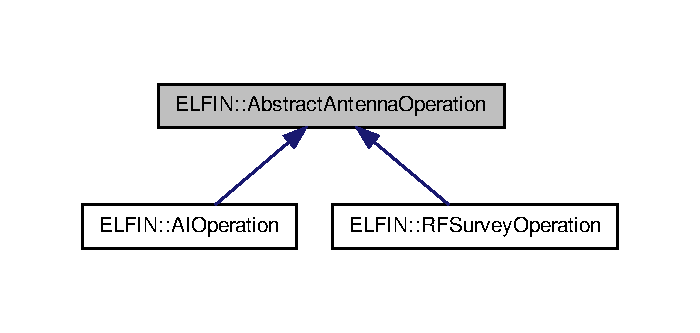
\includegraphics[width=336pt]{class_e_l_f_i_n_1_1_abstract_antenna_operation__inherit__graph}
\end{center}
\end{figure}


Collaboration diagram for E\-L\-F\-I\-N\-:\-:Abstract\-Antenna\-Operation\-:
\nopagebreak
\begin{figure}[H]
\begin{center}
\leavevmode
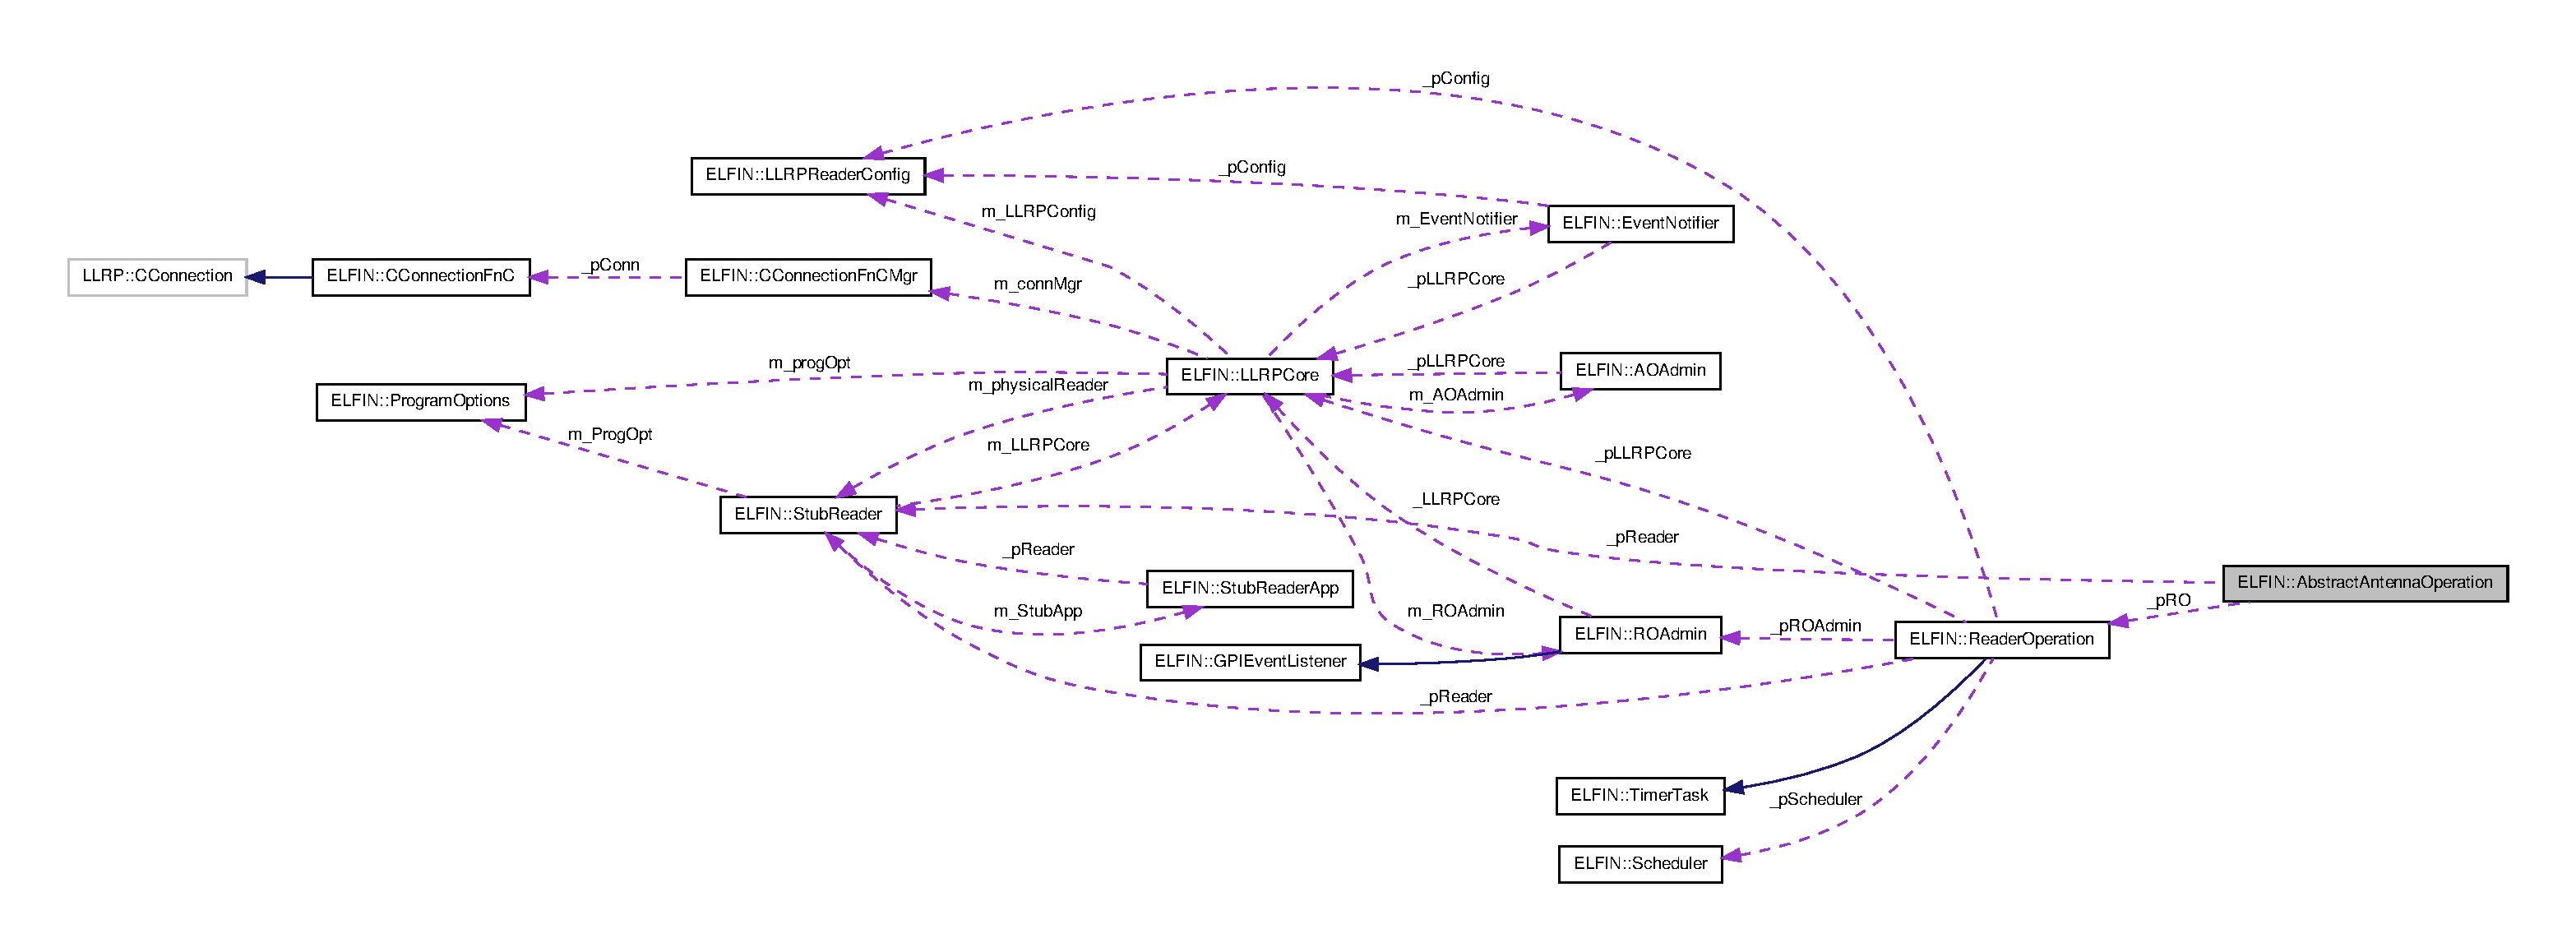
\includegraphics[width=350pt]{class_e_l_f_i_n_1_1_abstract_antenna_operation__coll__graph}
\end{center}
\end{figure}
\subsection*{Public Member Functions}
\begin{DoxyCompactItemize}
\item 
\hyperlink{class_e_l_f_i_n_1_1_abstract_antenna_operation_acbea0c1638717adb99062f3bc49c970e}{Abstract\-Antenna\-Operation} (\hyperlink{class_e_l_f_i_n_1_1_stub_reader}{Stub\-Reader} $\ast$\-\_\-\-\_\-p\-Reader, \hyperlink{class_e_l_f_i_n_1_1_reader_operation}{Reader\-Operation} $\ast$\-\_\-\-\_\-p\-R\-O, const L\-L\-R\-P\-::\-C\-Type\-Descriptor $\ast$p\-Type\-Descriptor, int \-\_\-\-\_\-p\-Spec\-Index)
\begin{DoxyCompactList}\small\item\em Constructor of \hyperlink{class_e_l_f_i_n_1_1_abstract_antenna_operation}{Abstract\-Antenna\-Operation} class. \end{DoxyCompactList}\item 
virtual \hyperlink{class_e_l_f_i_n_1_1_abstract_antenna_operation_a6c23f620e5d8c3831e584940c9cc8772}{$\sim$\-Abstract\-Antenna\-Operation} ()
\begin{DoxyCompactList}\small\item\em Destructor of \hyperlink{class_e_l_f_i_n_1_1_abstract_antenna_operation}{Abstract\-Antenna\-Operation} class. \end{DoxyCompactList}\item 
virtual Tag\-Report\-Set $\ast$ \hyperlink{class_e_l_f_i_n_1_1_abstract_antenna_operation_af8cd8a5e57d157a3af20c28c6e573bfb}{run} ()=0
\end{DoxyCompactItemize}
\subsection*{Public Attributes}
\begin{DoxyCompactItemize}
\item 
\hypertarget{class_e_l_f_i_n_1_1_abstract_antenna_operation_ae5270b59e19921d9007164ab6c2b5618}{\hyperlink{class_e_l_f_i_n_1_1_stub_reader}{Stub\-Reader} $\ast$ {\bfseries \-\_\-p\-Reader}}\label{class_e_l_f_i_n_1_1_abstract_antenna_operation_ae5270b59e19921d9007164ab6c2b5618}

\item 
\hyperlink{class_e_l_f_i_n_1_1_reader_operation}{Reader\-Operation} $\ast$ \hyperlink{class_e_l_f_i_n_1_1_abstract_antenna_operation_ae874826eb74270191459a48fae5a4131}{\-\_\-p\-R\-O}
\begin{DoxyCompactList}\small\item\em \hyperlink{class_e_l_f_i_n_1_1_reader_operation}{Reader\-Operation} which contains this operation. \end{DoxyCompactList}\item 
const L\-L\-R\-P\-::\-C\-Type\-Descriptor $\ast$ \hyperlink{class_e_l_f_i_n_1_1_abstract_antenna_operation_ae656ecd50678637a29a66743ceda3e86}{\-\_\-p\-Type\-Descriptor}
\begin{DoxyCompactList}\small\item\em Type descriptor of this operation. This is used to distinguish the type of this operation. \end{DoxyCompactList}\item 
\hypertarget{class_e_l_f_i_n_1_1_abstract_antenna_operation_a6c7ad0c0401080c3542ef9a68c0b3b4d}{int {\bfseries \-\_\-p\-Spec\-Index}}\label{class_e_l_f_i_n_1_1_abstract_antenna_operation_a6c7ad0c0401080c3542ef9a68c0b3b4d}

\end{DoxyCompactItemize}


\subsection{Detailed Description}
Abstraction for the classes which perform several operation with the antennas and tags. 

Definition at line 29 of file Abstract\-Antenna\-Operation.\-h.



\subsection{Constructor \& Destructor Documentation}
\hypertarget{class_e_l_f_i_n_1_1_abstract_antenna_operation_acbea0c1638717adb99062f3bc49c970e}{\index{E\-L\-F\-I\-N\-::\-Abstract\-Antenna\-Operation@{E\-L\-F\-I\-N\-::\-Abstract\-Antenna\-Operation}!Abstract\-Antenna\-Operation@{Abstract\-Antenna\-Operation}}
\index{Abstract\-Antenna\-Operation@{Abstract\-Antenna\-Operation}!ELFIN::AbstractAntennaOperation@{E\-L\-F\-I\-N\-::\-Abstract\-Antenna\-Operation}}
\subsubsection[{Abstract\-Antenna\-Operation}]{\setlength{\rightskip}{0pt plus 5cm}E\-L\-F\-I\-N\-::\-Abstract\-Antenna\-Operation\-::\-Abstract\-Antenna\-Operation (
\begin{DoxyParamCaption}
\item[{{\bf Stub\-Reader} $\ast$}]{\-\_\-\-\_\-p\-Reader, }
\item[{{\bf Reader\-Operation} $\ast$}]{\-\_\-\-\_\-p\-R\-O, }
\item[{const L\-L\-R\-P\-::\-C\-Type\-Descriptor $\ast$}]{p\-Type\-Descriptor, }
\item[{int}]{\-\_\-\-\_\-p\-Spec\-Index}
\end{DoxyParamCaption}
)}}\label{class_e_l_f_i_n_1_1_abstract_antenna_operation_acbea0c1638717adb99062f3bc49c970e}


Constructor of \hyperlink{class_e_l_f_i_n_1_1_abstract_antenna_operation}{Abstract\-Antenna\-Operation} class. 



Definition at line 8 of file Abstract\-Antenna\-Operation.\-cpp.

\hypertarget{class_e_l_f_i_n_1_1_abstract_antenna_operation_a6c23f620e5d8c3831e584940c9cc8772}{\index{E\-L\-F\-I\-N\-::\-Abstract\-Antenna\-Operation@{E\-L\-F\-I\-N\-::\-Abstract\-Antenna\-Operation}!$\sim$\-Abstract\-Antenna\-Operation@{$\sim$\-Abstract\-Antenna\-Operation}}
\index{$\sim$\-Abstract\-Antenna\-Operation@{$\sim$\-Abstract\-Antenna\-Operation}!ELFIN::AbstractAntennaOperation@{E\-L\-F\-I\-N\-::\-Abstract\-Antenna\-Operation}}
\subsubsection[{$\sim$\-Abstract\-Antenna\-Operation}]{\setlength{\rightskip}{0pt plus 5cm}virtual E\-L\-F\-I\-N\-::\-Abstract\-Antenna\-Operation\-::$\sim$\-Abstract\-Antenna\-Operation (
\begin{DoxyParamCaption}
{}
\end{DoxyParamCaption}
)\hspace{0.3cm}{\ttfamily [inline]}, {\ttfamily [virtual]}}}\label{class_e_l_f_i_n_1_1_abstract_antenna_operation_a6c23f620e5d8c3831e584940c9cc8772}


Destructor of \hyperlink{class_e_l_f_i_n_1_1_abstract_antenna_operation}{Abstract\-Antenna\-Operation} class. 



Definition at line 36 of file Abstract\-Antenna\-Operation.\-h.



\subsection{Member Function Documentation}
\hypertarget{class_e_l_f_i_n_1_1_abstract_antenna_operation_af8cd8a5e57d157a3af20c28c6e573bfb}{\index{E\-L\-F\-I\-N\-::\-Abstract\-Antenna\-Operation@{E\-L\-F\-I\-N\-::\-Abstract\-Antenna\-Operation}!run@{run}}
\index{run@{run}!ELFIN::AbstractAntennaOperation@{E\-L\-F\-I\-N\-::\-Abstract\-Antenna\-Operation}}
\subsubsection[{run}]{\setlength{\rightskip}{0pt plus 5cm}virtual Tag\-Report\-Set$\ast$ E\-L\-F\-I\-N\-::\-Abstract\-Antenna\-Operation\-::run (
\begin{DoxyParamCaption}
{}
\end{DoxyParamCaption}
)\hspace{0.3cm}{\ttfamily [pure virtual]}}}\label{class_e_l_f_i_n_1_1_abstract_antenna_operation_af8cd8a5e57d157a3af20c28c6e573bfb}
Performs the operation \begin{DoxyRefDesc}{Todo}
\item[\hyperlink{todo__todo000001}{Todo}]This should be fixed to conform \hyperlink{class_e_l_f_i_n_1_1_r_f_survey_operation}{R\-F\-Survey\-Operation}. \end{DoxyRefDesc}


Implemented in \hyperlink{class_e_l_f_i_n_1_1_a_i_operation_a13259c8516e1b5fb465e553c4c5dae01}{E\-L\-F\-I\-N\-::\-A\-I\-Operation}, and \hyperlink{class_e_l_f_i_n_1_1_r_f_survey_operation_a7eea340a95a2c04a7a93081354feeaf0}{E\-L\-F\-I\-N\-::\-R\-F\-Survey\-Operation}.



\subsection{Member Data Documentation}
\hypertarget{class_e_l_f_i_n_1_1_abstract_antenna_operation_ae874826eb74270191459a48fae5a4131}{\index{E\-L\-F\-I\-N\-::\-Abstract\-Antenna\-Operation@{E\-L\-F\-I\-N\-::\-Abstract\-Antenna\-Operation}!\-\_\-p\-R\-O@{\-\_\-p\-R\-O}}
\index{\-\_\-p\-R\-O@{\-\_\-p\-R\-O}!ELFIN::AbstractAntennaOperation@{E\-L\-F\-I\-N\-::\-Abstract\-Antenna\-Operation}}
\subsubsection[{\-\_\-p\-R\-O}]{\setlength{\rightskip}{0pt plus 5cm}{\bf Reader\-Operation}$\ast$ E\-L\-F\-I\-N\-::\-Abstract\-Antenna\-Operation\-::\-\_\-p\-R\-O}}\label{class_e_l_f_i_n_1_1_abstract_antenna_operation_ae874826eb74270191459a48fae5a4131}


\hyperlink{class_e_l_f_i_n_1_1_reader_operation}{Reader\-Operation} which contains this operation. 



Definition at line 39 of file Abstract\-Antenna\-Operation.\-h.

\hypertarget{class_e_l_f_i_n_1_1_abstract_antenna_operation_ae656ecd50678637a29a66743ceda3e86}{\index{E\-L\-F\-I\-N\-::\-Abstract\-Antenna\-Operation@{E\-L\-F\-I\-N\-::\-Abstract\-Antenna\-Operation}!\-\_\-p\-Type\-Descriptor@{\-\_\-p\-Type\-Descriptor}}
\index{\-\_\-p\-Type\-Descriptor@{\-\_\-p\-Type\-Descriptor}!ELFIN::AbstractAntennaOperation@{E\-L\-F\-I\-N\-::\-Abstract\-Antenna\-Operation}}
\subsubsection[{\-\_\-p\-Type\-Descriptor}]{\setlength{\rightskip}{0pt plus 5cm}const L\-L\-R\-P\-::\-C\-Type\-Descriptor$\ast$ E\-L\-F\-I\-N\-::\-Abstract\-Antenna\-Operation\-::\-\_\-p\-Type\-Descriptor}}\label{class_e_l_f_i_n_1_1_abstract_antenna_operation_ae656ecd50678637a29a66743ceda3e86}


Type descriptor of this operation. This is used to distinguish the type of this operation. 



Definition at line 41 of file Abstract\-Antenna\-Operation.\-h.



The documentation for this class was generated from the following files\-:\begin{DoxyCompactItemize}
\item 
elfin\-\_\-src/\hyperlink{_abstract_antenna_operation_8h}{Abstract\-Antenna\-Operation.\-h}\item 
elfin\-\_\-src/\hyperlink{_abstract_antenna_operation_8cpp}{Abstract\-Antenna\-Operation.\-cpp}\end{DoxyCompactItemize}

\hypertarget{class_e_l_f_i_n_1_1_abstract_reader}{\section{E\-L\-F\-I\-N\-:\-:Abstract\-Reader Class Reference}
\label{class_e_l_f_i_n_1_1_abstract_reader}\index{E\-L\-F\-I\-N\-::\-Abstract\-Reader@{E\-L\-F\-I\-N\-::\-Abstract\-Reader}}
}


Inheritance diagram for E\-L\-F\-I\-N\-:\-:Abstract\-Reader\-:
\nopagebreak
\begin{figure}[H]
\begin{center}
\leavevmode
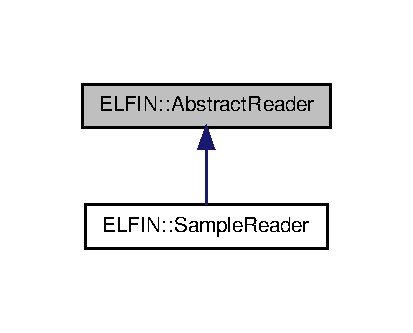
\includegraphics[width=198pt]{class_e_l_f_i_n_1_1_abstract_reader__inherit__graph}
\end{center}
\end{figure}


Collaboration diagram for E\-L\-F\-I\-N\-:\-:Abstract\-Reader\-:
\nopagebreak
\begin{figure}[H]
\begin{center}
\leavevmode
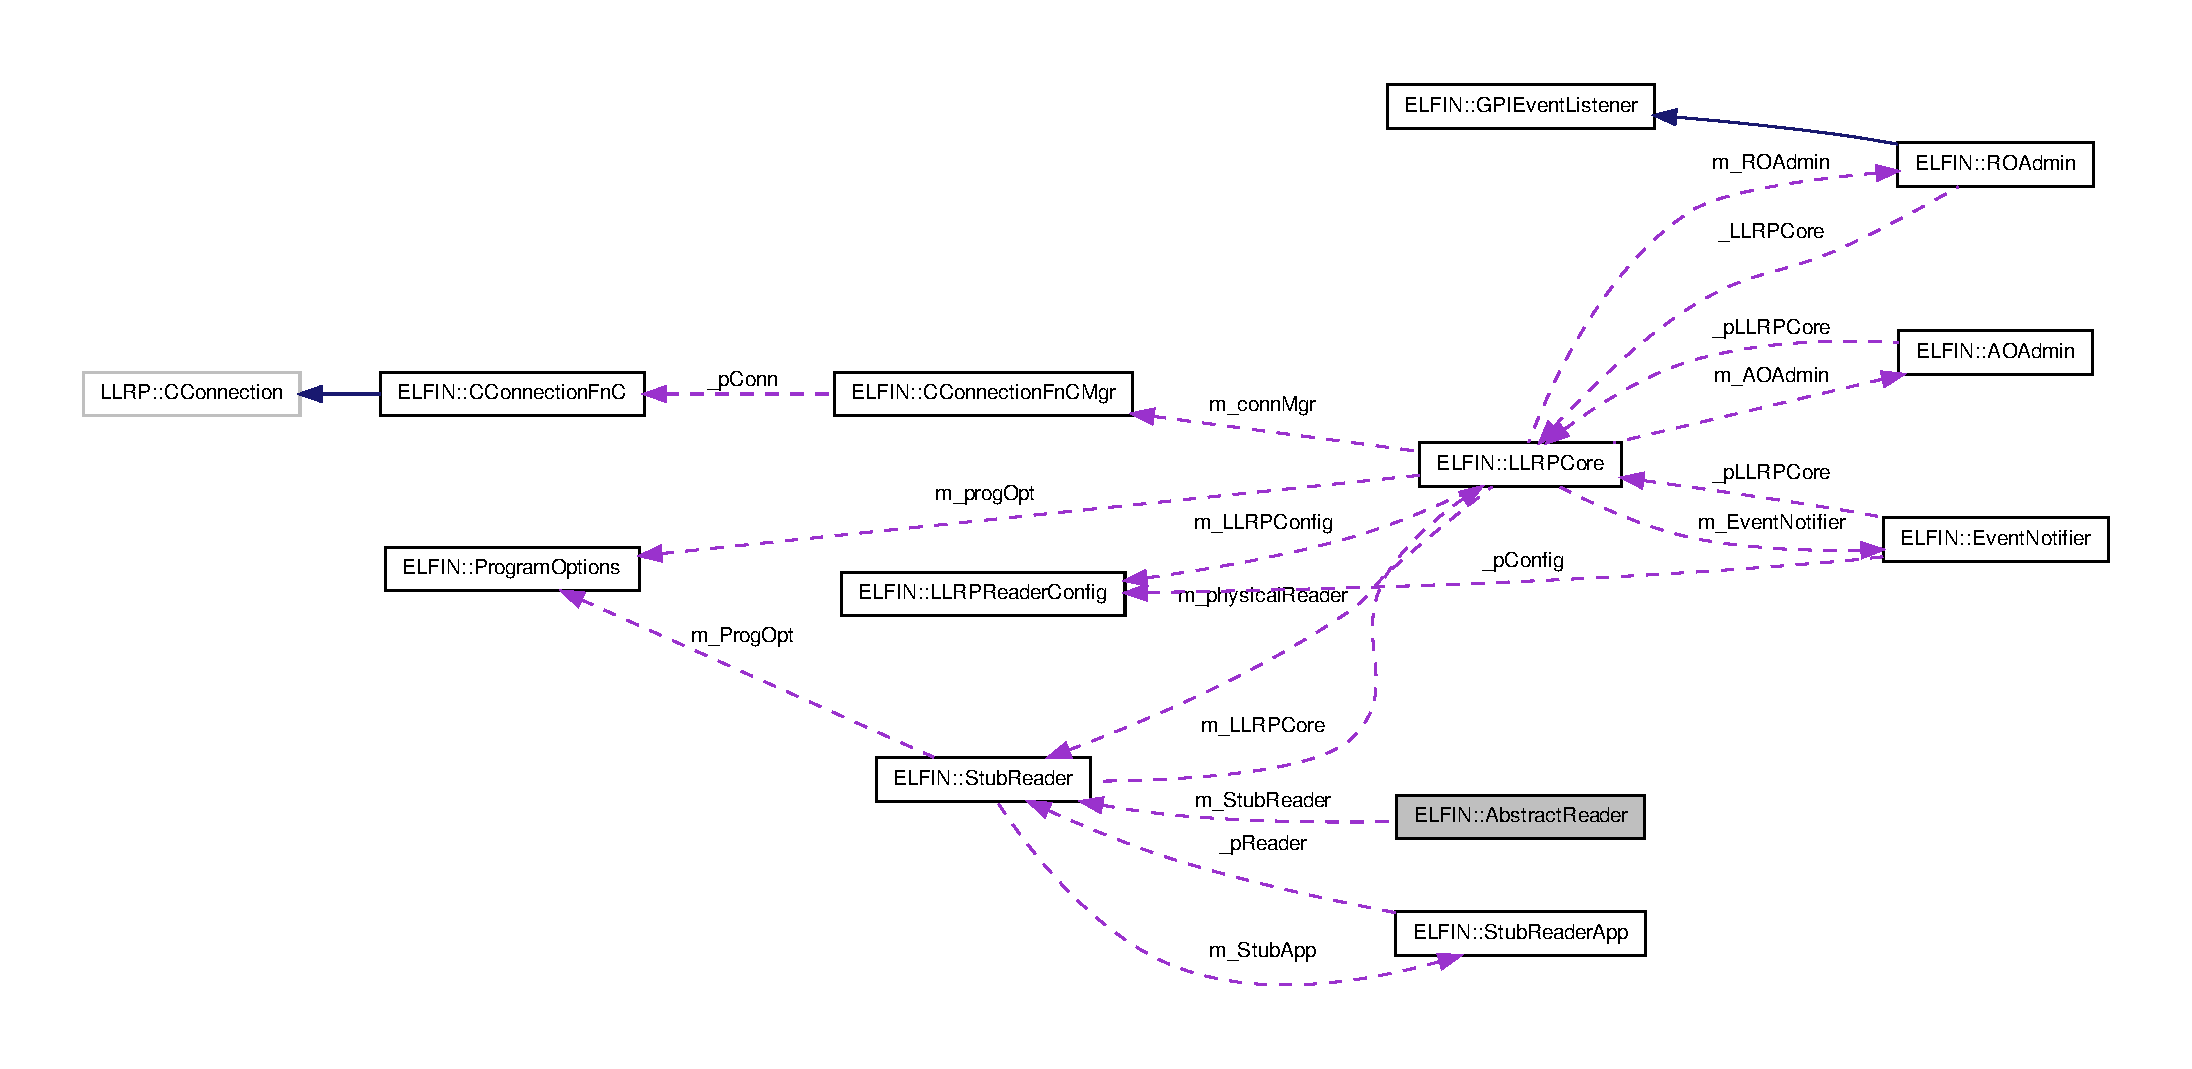
\includegraphics[width=350pt]{class_e_l_f_i_n_1_1_abstract_reader__coll__graph}
\end{center}
\end{figure}
\subsection*{Public Member Functions}
\begin{DoxyCompactItemize}
\item 
\hypertarget{class_e_l_f_i_n_1_1_abstract_reader_aa1be28f1bf872f36ccbb53b2dbb83ff5}{{\bfseries Abstract\-Reader} (\hyperlink{class_e_l_f_i_n_1_1_stub_reader}{Stub\-Reader} $\ast$a\-\_\-\-Stub\-Reader)}\label{class_e_l_f_i_n_1_1_abstract_reader_aa1be28f1bf872f36ccbb53b2dbb83ff5}

\item 
\hypertarget{class_e_l_f_i_n_1_1_abstract_reader_a8d7535f318d134739c081d745670b51b}{virtual E\-L\-F\-I\-N\-::\-Tag\-Vector $\ast$ {\bfseries get\-Current\-Tags} (bool R\-S\-S\-I\-Enabled)=0}\label{class_e_l_f_i_n_1_1_abstract_reader_a8d7535f318d134739c081d745670b51b}

\item 
\hypertarget{class_e_l_f_i_n_1_1_abstract_reader_a155474dd8622c3a87566c579d1bacedb}{int {\bfseries \-\_\-start\-Tag\-Read} (int read\-Cycle)}\label{class_e_l_f_i_n_1_1_abstract_reader_a155474dd8622c3a87566c579d1bacedb}

\item 
\hypertarget{class_e_l_f_i_n_1_1_abstract_reader_ab3da76dbe35618e6f8c8eb70b709df59}{int {\bfseries \-\_\-stop\-Tag\-Read} ()}\label{class_e_l_f_i_n_1_1_abstract_reader_ab3da76dbe35618e6f8c8eb70b709df59}

\item 
\hypertarget{class_e_l_f_i_n_1_1_abstract_reader_ac4dd47850c2ea685aec7f04acd14eb65}{int {\bfseries \-\_\-read\-Tag\-Memory} (uint16\-\_\-t access\-Password, uint16\-\_\-t epc\-Length, char $\ast$epc, uint16\-\_\-t memory\-Bank, uint16\-\_\-t start\-Address, uint16\-\_\-t data\-Length)}\label{class_e_l_f_i_n_1_1_abstract_reader_ac4dd47850c2ea685aec7f04acd14eb65}

\item 
\hypertarget{class_e_l_f_i_n_1_1_abstract_reader_a75b16c903f66dc0c697fbad503eecf72}{int {\bfseries \-\_\-write\-Tag\-Memory} (uint16\-\_\-t access\-Password, uint16\-\_\-t epc\-Length, char $\ast$epc, uint16\-\_\-t memory\-Bank, uint16\-\_\-t start\-Address, uint16\-\_\-t data\-Length, char $\ast$data\-To\-Write)}\label{class_e_l_f_i_n_1_1_abstract_reader_a75b16c903f66dc0c697fbad503eecf72}

\item 
\hypertarget{class_e_l_f_i_n_1_1_abstract_reader_a7de97c2cd661bbcb72a80da4d3d9b7d4}{int {\bfseries \-\_\-lock\-Tag\-Memory} ()}\label{class_e_l_f_i_n_1_1_abstract_reader_a7de97c2cd661bbcb72a80da4d3d9b7d4}

\item 
\hypertarget{class_e_l_f_i_n_1_1_abstract_reader_a53e08b085014d4e3c79d1a4078e27c55}{int {\bfseries \-\_\-kill\-Tag\-Memory} ()}\label{class_e_l_f_i_n_1_1_abstract_reader_a53e08b085014d4e3c79d1a4078e27c55}

\item 
\hypertarget{class_e_l_f_i_n_1_1_abstract_reader_a09ef7e8697a076ffdc49d8dbb5d58e93}{int {\bfseries reg\-Tag\-Callback} (boost\-::function$<$ int(\hyperlink{class_e_l_f_i_n_1_1_stub_reader}{Stub\-Reader} $\ast$, \hyperlink{class_e_l_f_i_n_1_1_stub_tag}{Stub\-Tag} $\ast$)$>$ p\-Tag\-Call\-Back)}\label{class_e_l_f_i_n_1_1_abstract_reader_a09ef7e8697a076ffdc49d8dbb5d58e93}

\item 
\hypertarget{class_e_l_f_i_n_1_1_abstract_reader_ae6fc040fd2a28baf7409c9bff1259197}{virtual int {\bfseries init} ()=0}\label{class_e_l_f_i_n_1_1_abstract_reader_ae6fc040fd2a28baf7409c9bff1259197}

\item 
\hypertarget{class_e_l_f_i_n_1_1_abstract_reader_a21fbc506ee7e9b952bc908a85fd54169}{virtual int {\bfseries start\-Tag\-Read} (int read\-Cycle)=0}\label{class_e_l_f_i_n_1_1_abstract_reader_a21fbc506ee7e9b952bc908a85fd54169}

\item 
\hypertarget{class_e_l_f_i_n_1_1_abstract_reader_afa744bda4c0515ad16231ce51f13ee29}{virtual int {\bfseries stop\-Tag\-Read} ()=0}\label{class_e_l_f_i_n_1_1_abstract_reader_afa744bda4c0515ad16231ce51f13ee29}

\item 
\hypertarget{class_e_l_f_i_n_1_1_abstract_reader_a7b78ab281237c7eb70e7d0874c483dac}{virtual int {\bfseries read\-Tag\-Memory} (uint16\-\_\-t access\-Password, uint16\-\_\-t epc\-Length, char $\ast$epc, uint16\-\_\-t memory\-Bank, uint16\-\_\-t start\-Address, uint16\-\_\-t data\-Length)=0}\label{class_e_l_f_i_n_1_1_abstract_reader_a7b78ab281237c7eb70e7d0874c483dac}

\item 
\hypertarget{class_e_l_f_i_n_1_1_abstract_reader_a08385c75c19fef14eb72a94372fb904d}{virtual int {\bfseries write\-Tag\-Memory} (uint16\-\_\-t access\-Password, uint16\-\_\-t epc\-Length, char $\ast$epc, uint16\-\_\-t memory\-Bank, uint16\-\_\-t start\-Address, uint16\-\_\-t data\-Length, char $\ast$data\-To\-Write)=0}\label{class_e_l_f_i_n_1_1_abstract_reader_a08385c75c19fef14eb72a94372fb904d}

\end{DoxyCompactItemize}
\subsection*{Public Attributes}
\begin{DoxyCompactItemize}
\item 
\hypertarget{class_e_l_f_i_n_1_1_abstract_reader_ac66092c17c0c8ab77e9112d47dfddd1c}{boost\-::recursive\-\_\-mutex {\bfseries m\-\_\-\-Abstract\-Reader\-Lock}}\label{class_e_l_f_i_n_1_1_abstract_reader_ac66092c17c0c8ab77e9112d47dfddd1c}

\item 
\hypertarget{class_e_l_f_i_n_1_1_abstract_reader_a07ce3410eb4612dc3bcda179f0b1ac3c}{int {\bfseries m\-\_\-\-Read\-Command\-Count}}\label{class_e_l_f_i_n_1_1_abstract_reader_a07ce3410eb4612dc3bcda179f0b1ac3c}

\item 
\hypertarget{class_e_l_f_i_n_1_1_abstract_reader_a73c8d1e5ec82d59ec8dd484dfd872e8c}{boost\-::function$<$ int(\hyperlink{class_e_l_f_i_n_1_1_stub_reader}{Stub\-Reader} \\*
$\ast$, \hyperlink{class_e_l_f_i_n_1_1_stub_tag}{Stub\-Tag} $\ast$)$>$ {\bfseries m\-\_\-tag\-Call\-Back}}\label{class_e_l_f_i_n_1_1_abstract_reader_a73c8d1e5ec82d59ec8dd484dfd872e8c}

\end{DoxyCompactItemize}
\subsection*{Protected Attributes}
\begin{DoxyCompactItemize}
\item 
\hypertarget{class_e_l_f_i_n_1_1_abstract_reader_aa1de5d53b34213146ea82b150e6c740b}{\hyperlink{class_e_l_f_i_n_1_1_stub_reader}{Stub\-Reader} $\ast$ {\bfseries m\-\_\-\-Stub\-Reader}}\label{class_e_l_f_i_n_1_1_abstract_reader_aa1de5d53b34213146ea82b150e6c740b}

\end{DoxyCompactItemize}


\subsection{Detailed Description}


Definition at line 15 of file Abstract\-Reader.\-h.



The documentation for this class was generated from the following file\-:\begin{DoxyCompactItemize}
\item 
elfin\-\_\-src/\-Reader\-Handler/Abstract\-Reader.\-h\end{DoxyCompactItemize}

\hypertarget{class_e_l_f_i_n_1_1_abstract_trigger}{\section{E\-L\-F\-I\-N\-:\-:Abstract\-Trigger Class Reference}
\label{class_e_l_f_i_n_1_1_abstract_trigger}\index{E\-L\-F\-I\-N\-::\-Abstract\-Trigger@{E\-L\-F\-I\-N\-::\-Abstract\-Trigger}}
}


Inheritance diagram for E\-L\-F\-I\-N\-:\-:Abstract\-Trigger\-:
\nopagebreak
\begin{figure}[H]
\begin{center}
\leavevmode
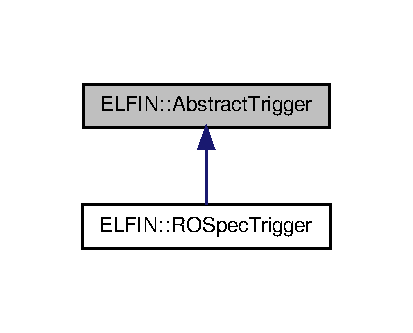
\includegraphics[width=198pt]{class_e_l_f_i_n_1_1_abstract_trigger__inherit__graph}
\end{center}
\end{figure}
\subsection*{Public Member Functions}
\begin{DoxyCompactItemize}
\item 
\hypertarget{class_e_l_f_i_n_1_1_abstract_trigger_a5633a30d5723b97c8474e7421151e473}{void {\bfseries enable\-Trigger} ()}\label{class_e_l_f_i_n_1_1_abstract_trigger_a5633a30d5723b97c8474e7421151e473}

\item 
\hypertarget{class_e_l_f_i_n_1_1_abstract_trigger_ac70002a59acc7aee6947f946f3387eb2}{void {\bfseries disable\-Trigger} ()}\label{class_e_l_f_i_n_1_1_abstract_trigger_ac70002a59acc7aee6947f946f3387eb2}

\item 
\hypertarget{class_e_l_f_i_n_1_1_abstract_trigger_a5c614add4625141d220645268afcf2c6}{void {\bfseries fire\-Trigger} ()}\label{class_e_l_f_i_n_1_1_abstract_trigger_a5c614add4625141d220645268afcf2c6}

\item 
\hypertarget{class_e_l_f_i_n_1_1_abstract_trigger_aadea65da88b0ceb8d807e5e5863e1ad6}{int {\bfseries is\-Fired} ()}\label{class_e_l_f_i_n_1_1_abstract_trigger_aadea65da88b0ceb8d807e5e5863e1ad6}

\item 
\hypertarget{class_e_l_f_i_n_1_1_abstract_trigger_a5e82d5eb6d1380e22569eb528c1f86fc}{void {\bfseries observed\-New\-Tag\-Callback} ()}\label{class_e_l_f_i_n_1_1_abstract_trigger_a5e82d5eb6d1380e22569eb528c1f86fc}

\item 
\hypertarget{class_e_l_f_i_n_1_1_abstract_trigger_a34a7e5a8fd3e3482b5e17e3369360d42}{void {\bfseries create\-Timeout} (int wait\-M\-S)}\label{class_e_l_f_i_n_1_1_abstract_trigger_a34a7e5a8fd3e3482b5e17e3369360d42}

\item 
\hypertarget{class_e_l_f_i_n_1_1_abstract_trigger_a503210754bef556363fdf0bad5a4a214}{void {\bfseries deadline\-Timer\-Handler} (const boost\-::system\-::error\-\_\-code \&e)}\label{class_e_l_f_i_n_1_1_abstract_trigger_a503210754bef556363fdf0bad5a4a214}

\end{DoxyCompactItemize}
\subsection*{Protected Attributes}
\begin{DoxyCompactItemize}
\item 
\hypertarget{class_e_l_f_i_n_1_1_abstract_trigger_a90e6454e493094e5295a8d71871f71a7}{int {\bfseries m\-\_\-is\-Fired}}\label{class_e_l_f_i_n_1_1_abstract_trigger_a90e6454e493094e5295a8d71871f71a7}

\item 
\hypertarget{class_e_l_f_i_n_1_1_abstract_trigger_ae13c310832134d6bad0e802ad767b56b}{int {\bfseries m\-\_\-time\-Out}}\label{class_e_l_f_i_n_1_1_abstract_trigger_ae13c310832134d6bad0e802ad767b56b}

\item 
\hypertarget{class_e_l_f_i_n_1_1_abstract_trigger_a9c0feec8187fe38904acd46b860965bf}{int {\bfseries m\-\_\-tag\-Count}}\label{class_e_l_f_i_n_1_1_abstract_trigger_a9c0feec8187fe38904acd46b860965bf}

\item 
\hypertarget{class_e_l_f_i_n_1_1_abstract_trigger_aa1403adec2d6ca774838148f7bf19be3}{int {\bfseries m\-\_\-tag\-Count\-Limit}}\label{class_e_l_f_i_n_1_1_abstract_trigger_aa1403adec2d6ca774838148f7bf19be3}

\item 
\hypertarget{class_e_l_f_i_n_1_1_abstract_trigger_a1ef218ddb60371959e0bcf1f315ef6d6}{boost\-::asio\-::io\-\_\-service {\bfseries m\-\_\-ios}}\label{class_e_l_f_i_n_1_1_abstract_trigger_a1ef218ddb60371959e0bcf1f315ef6d6}

\item 
\hypertarget{class_e_l_f_i_n_1_1_abstract_trigger_a85be320c6b145a89a188647809a24f77}{boost\-::asio\-::deadline\-\_\-timer $\ast$ {\bfseries m\-\_\-timer}}\label{class_e_l_f_i_n_1_1_abstract_trigger_a85be320c6b145a89a188647809a24f77}

\end{DoxyCompactItemize}


\subsection{Detailed Description}


Definition at line 14 of file Abstract\-Trigger.\-h.



The documentation for this class was generated from the following file\-:\begin{DoxyCompactItemize}
\item 
elfin\-\_\-src/\-Triggers/\hyperlink{_abstract_trigger_8h}{Abstract\-Trigger.\-h}\end{DoxyCompactItemize}

\hypertarget{class_e_l_f_i_n_1_1_access_operation}{\section{E\-L\-F\-I\-N\-:\-:Access\-Operation Class Reference}
\label{class_e_l_f_i_n_1_1_access_operation}\index{E\-L\-F\-I\-N\-::\-Access\-Operation@{E\-L\-F\-I\-N\-::\-Access\-Operation}}
}


A single access operation generated based on the given Access\-Spec parameter.  




{\ttfamily \#include $<$Access\-Operation.\-h$>$}



Collaboration diagram for E\-L\-F\-I\-N\-:\-:Access\-Operation\-:
\nopagebreak
\begin{figure}[H]
\begin{center}
\leavevmode
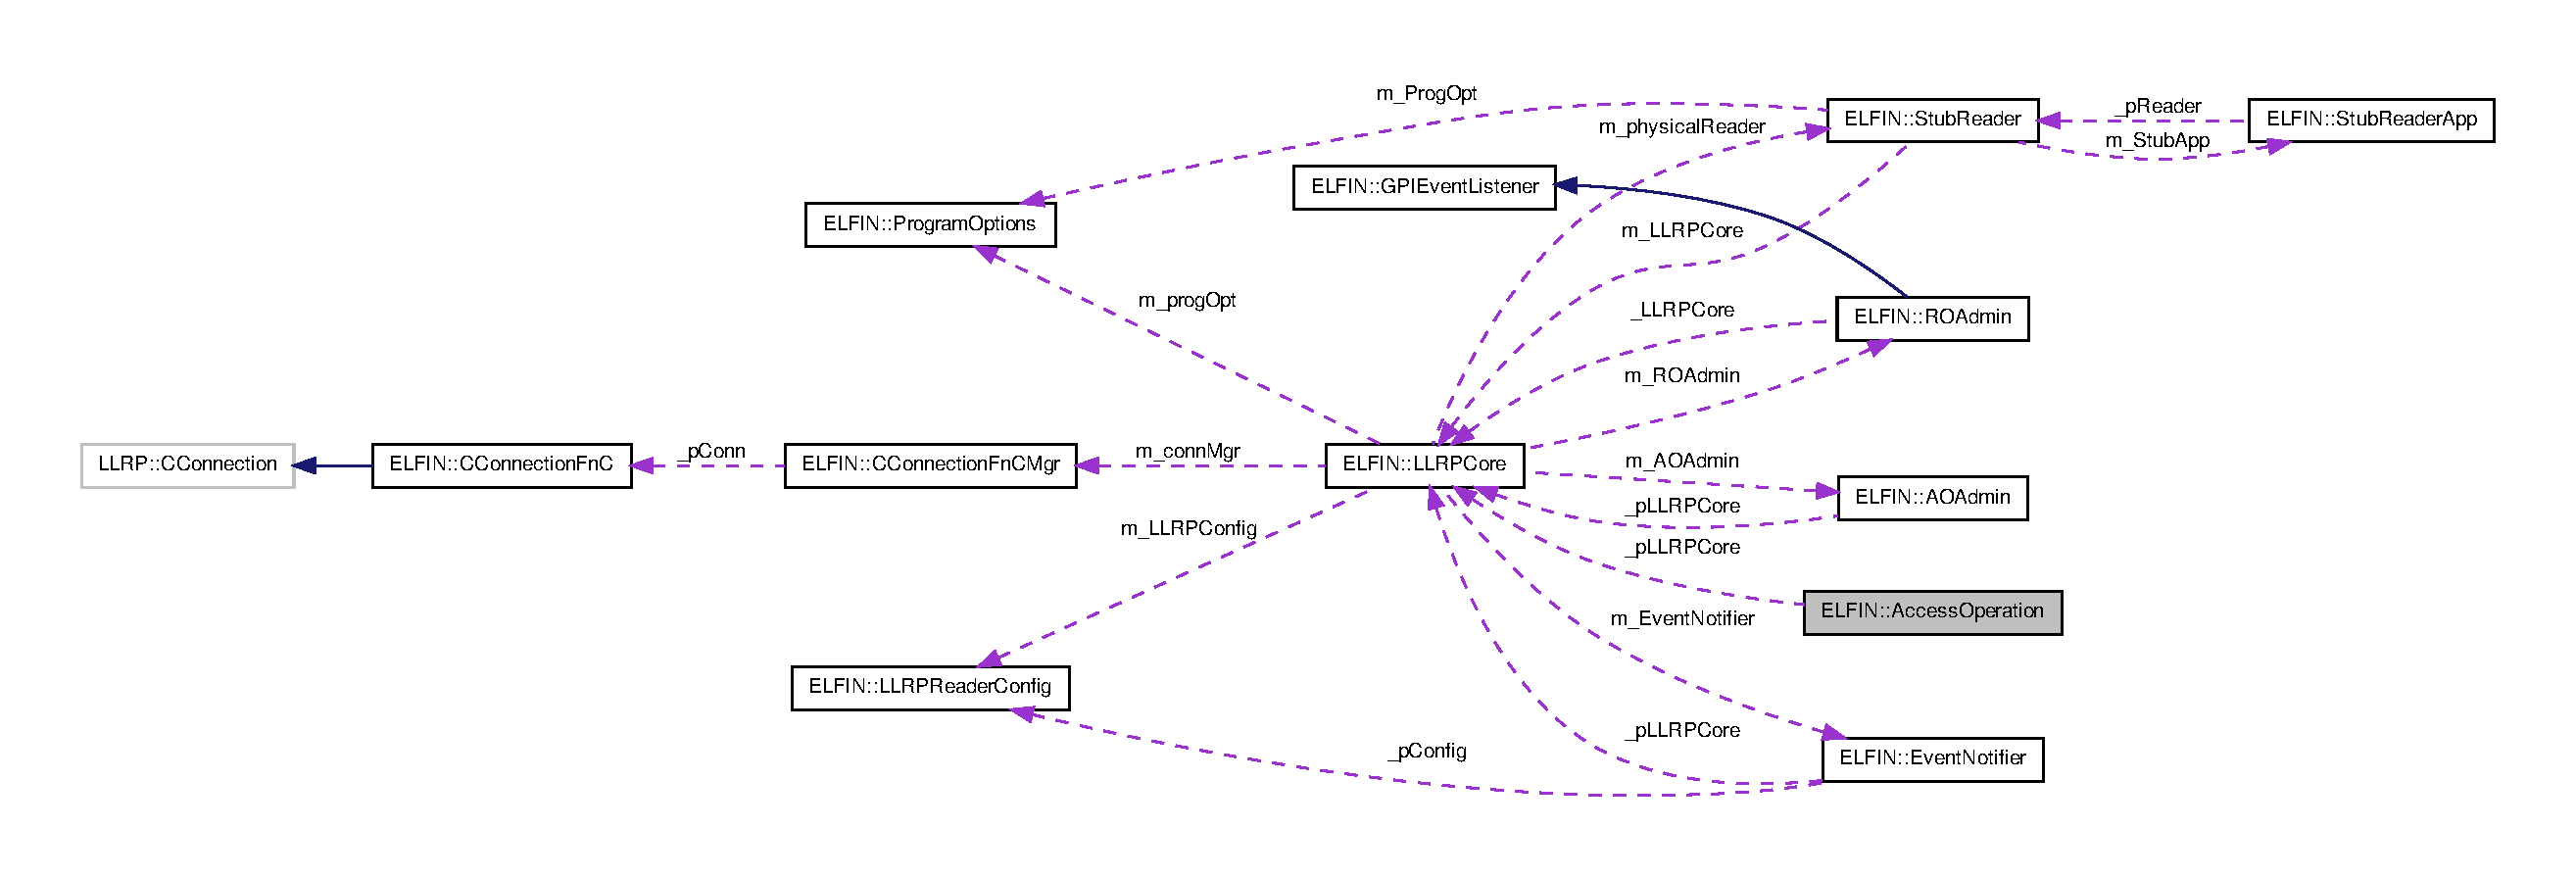
\includegraphics[width=350pt]{class_e_l_f_i_n_1_1_access_operation__coll__graph}
\end{center}
\end{figure}
\subsection*{Public Member Functions}
\begin{DoxyCompactItemize}
\item 
\hyperlink{class_e_l_f_i_n_1_1_access_operation_ac2138a56bbd039b4d5c2354ddda25992}{Access\-Operation} (\hyperlink{class_e_l_f_i_n_1_1_l_l_r_p_core}{L\-L\-R\-P\-Core} $\ast$\-\_\-\-\_\-p\-L\-L\-R\-P\-Core, L\-L\-R\-P\-::\-C\-Access\-Spec $\ast$\-\_\-\-\_\-p\-C\-Access\-Spec)
\begin{DoxyCompactList}\small\item\em Constructor of \hyperlink{class_e_l_f_i_n_1_1_access_operation}{Access\-Operation} class. \end{DoxyCompactList}\item 
int \hyperlink{class_e_l_f_i_n_1_1_access_operation_abd6ee0b2cb143103440bd9caed9dff19}{is\-Valid} ()
\begin{DoxyCompactList}\small\item\em Check the validity of \hyperlink{class_e_l_f_i_n_1_1_access_operation}{Access\-Operation} object. \end{DoxyCompactList}\item 
int \hyperlink{class_e_l_f_i_n_1_1_access_operation_a9f928363dd0ab1a6a0ef2f3e594e60a4}{match\-Tag\-Spec} (\hyperlink{class_e_l_f_i_n_1_1_stub_tag}{Stub\-Tag} $\ast$p\-Stub\-Tag, L\-L\-R\-P\-::llrp\-\_\-u32\-\_\-t p\-R\-O\-Spec\-I\-D)
\begin{DoxyCompactList}\small\item\em Match the provided \hyperlink{class_e_l_f_i_n_1_1_stub_tag}{Stub\-Tag} and R\-O\-Spec\-I\-D to the current C1\-G2\-Target\-Tag. \end{DoxyCompactList}\item 
int \hyperlink{class_e_l_f_i_n_1_1_access_operation_a7b21dfebb3248fe9e4105c8dca4ce897}{execute\-Op\-Specs} (\hyperlink{class_e_l_f_i_n_1_1_stub_tag}{Stub\-Tag} $\ast$p\-Stub\-Tag, L\-L\-R\-P\-::\-C\-Tag\-Report\-Data $\ast$p\-Tag\-Report)
\begin{DoxyCompactList}\small\item\em Apply Op\-Spec to the provided \hyperlink{class_e_l_f_i_n_1_1_stub_tag}{Stub\-Tag}. The Op\-Spec\-Result would be stored to the p\-Tag\-Report object. \end{DoxyCompactList}\item 
int \hyperlink{class_e_l_f_i_n_1_1_access_operation_af944ff98cc959755f16f892ef1be7559}{handle\-C1\-G2\-Read} (L\-L\-R\-P\-::\-C\-Access\-Command\-Op\-Spec $\ast$p\-Op\-Spec, \hyperlink{class_e_l_f_i_n_1_1_stub_tag}{Stub\-Tag} $\ast$p\-Stub\-Tag, L\-L\-R\-P\-::\-C\-Tag\-Report\-Data $\ast$p\-Tag\-Report)
\begin{DoxyCompactList}\small\item\em Handles C1\-G2\-Read Op\-Spec. The result is stored to the p\-Tag\-Report object. \end{DoxyCompactList}\item 
int \hyperlink{class_e_l_f_i_n_1_1_access_operation_a019256d2d181eec3688845227ed50a62}{handle\-C1\-G2\-Write} (L\-L\-R\-P\-::\-C\-Access\-Command\-Op\-Spec $\ast$p\-Op\-Spec, \hyperlink{class_e_l_f_i_n_1_1_stub_tag}{Stub\-Tag} $\ast$p\-Stub\-Tag, L\-L\-R\-P\-::\-C\-Tag\-Report\-Data $\ast$p\-Tag\-Report)
\begin{DoxyCompactList}\small\item\em Handles C1\-G2\-Write Op\-Spec. The result is stored to the p\-Tag\-Report object. \end{DoxyCompactList}\end{DoxyCompactItemize}
{\bf }\par
\begin{DoxyCompactItemize}
\item 
int \hyperlink{class_e_l_f_i_n_1_1_access_operation_aaa62c42a3e98fdb8a583a16561c4d416}{handle\-C1\-G2\-Kill} (L\-L\-R\-P\-::\-C\-Access\-Command\-Op\-Spec $\ast$p\-Op\-Spec, \hyperlink{class_e_l_f_i_n_1_1_stub_tag}{Stub\-Tag} $\ast$p\-Stub\-Tag, L\-L\-R\-P\-::\-C\-Tag\-Report\-Data $\ast$p\-Tag\-Report)
\begin{DoxyCompactList}\small\item\em Handles corresponding Op\-Spec. But this method is not implemented yet. \end{DoxyCompactList}\item 
int \hyperlink{class_e_l_f_i_n_1_1_access_operation_a0fccaea52a98abc72788c6fe7b5bbe2d}{handle\-C1\-G2\-Lock} (L\-L\-R\-P\-::\-C\-Access\-Command\-Op\-Spec $\ast$p\-Op\-Spec, \hyperlink{class_e_l_f_i_n_1_1_stub_tag}{Stub\-Tag} $\ast$p\-Stub\-Tag, L\-L\-R\-P\-::\-C\-Tag\-Report\-Data $\ast$p\-Tag\-Report)
\begin{DoxyCompactList}\small\item\em Handles corresponding Op\-Spec. But this method is not implemented yet. \end{DoxyCompactList}\item 
int \hyperlink{class_e_l_f_i_n_1_1_access_operation_aa7a89cb757c2d02c222a5a68703c3fd7}{handle\-C1\-G2\-Block\-Erase} (L\-L\-R\-P\-::\-C\-Access\-Command\-Op\-Spec $\ast$p\-Op\-Spec, \hyperlink{class_e_l_f_i_n_1_1_stub_tag}{Stub\-Tag} $\ast$p\-Stub\-Tag, L\-L\-R\-P\-::\-C\-Tag\-Report\-Data $\ast$p\-Tag\-Report)
\begin{DoxyCompactList}\small\item\em Handles corresponding Op\-Spec. But this method is not implemented yet. \end{DoxyCompactList}\item 
int \hyperlink{class_e_l_f_i_n_1_1_access_operation_a33d4d046de073308c854a5e16595197f}{handle\-C1\-G2\-Block\-Write} (L\-L\-R\-P\-::\-C\-Access\-Command\-Op\-Spec $\ast$p\-Op\-Spec, \hyperlink{class_e_l_f_i_n_1_1_stub_tag}{Stub\-Tag} $\ast$p\-Stub\-Tag, L\-L\-R\-P\-::\-C\-Tag\-Report\-Data $\ast$p\-Tag\-Report)
\begin{DoxyCompactList}\small\item\em Handles corresponding Op\-Spec. But this method is not implemented yet. \end{DoxyCompactList}\end{DoxyCompactItemize}

\subsection*{Static Public Member Functions}
\begin{DoxyCompactItemize}
\item 
static L\-L\-R\-P\-::llrp\-\_\-u16\-\_\-t \hyperlink{class_e_l_f_i_n_1_1_access_operation_a153d7378aa347f667b22a2a170837622}{get\-Op\-Spec\-I\-D} (L\-L\-R\-P\-::\-C\-Access\-Command\-Op\-Spec $\ast$p\-Op\-Spec)
\begin{DoxyCompactList}\small\item\em Get the Op\-Spec id from the given Op\-Spec. \end{DoxyCompactList}\item 
static L\-L\-R\-P\-::llrp\-\_\-u16\-\_\-t \hyperlink{class_e_l_f_i_n_1_1_access_operation_a779c7cc8692989b0b1bc5789cef29e5b}{get\-A\-C\-Op\-Spec\-Result\-O\-P\-Spec\-I\-D} (L\-L\-R\-P\-::\-C\-Access\-Command\-Op\-Spec\-Result $\ast$p\-Access\-Command\-Op\-Spec\-Result)
\begin{DoxyCompactList}\small\item\em Get the Op\-Spec id from the given Access\-Command\-Op\-Spec\-Result. \end{DoxyCompactList}\item 
static int \hyperlink{class_e_l_f_i_n_1_1_access_operation_a7f5fbbbd2e32941d87c0f296d9869dd4}{compare\-A\-C\-Op\-Spec\-Result} (L\-L\-R\-P\-::\-C\-Access\-Command\-Op\-Spec\-Result $\ast$p\-Result1, L\-L\-R\-P\-::\-C\-Access\-Command\-Op\-Spec\-Result $\ast$p\-Result2)
\begin{DoxyCompactList}\small\item\em Compare two C\-Access\-Command\-Op\-Spec\-Result. If they are identical, returns 0. If not, returns non-\/zero value. \end{DoxyCompactList}\end{DoxyCompactItemize}
\subsection*{Public Attributes}
\begin{DoxyCompactItemize}
\item 
\hypertarget{class_e_l_f_i_n_1_1_access_operation_a6b116c469b2c6d8bed6d8436cfa9ed4b}{\hyperlink{class_e_l_f_i_n_1_1_l_l_r_p_core}{L\-L\-R\-P\-Core} $\ast$ {\bfseries \-\_\-p\-L\-L\-R\-P\-Core}}\label{class_e_l_f_i_n_1_1_access_operation_a6b116c469b2c6d8bed6d8436cfa9ed4b}

\item 
\hypertarget{class_e_l_f_i_n_1_1_access_operation_aff207b159e862557b1c9b56a377dd8bf}{L\-L\-R\-P\-::\-C\-Access\-Spec $\ast$ {\bfseries \-\_\-p\-C\-Access\-Spec}}\label{class_e_l_f_i_n_1_1_access_operation_aff207b159e862557b1c9b56a377dd8bf}

\item 
\hypertarget{class_e_l_f_i_n_1_1_access_operation_a68385342f946fc8d8815e13b26c05297}{L\-L\-R\-P\-::\-C\-Access\-Report\-Spec $\ast$ {\bfseries \-\_\-p\-Access\-Report\-Spec}}\label{class_e_l_f_i_n_1_1_access_operation_a68385342f946fc8d8815e13b26c05297}

\item 
\hypertarget{class_e_l_f_i_n_1_1_access_operation_af20d9e59c1a139f459f8e6c250d7941c}{L\-L\-R\-P\-::\-C\-C1\-G2\-Tag\-Spec $\ast$ {\bfseries \-\_\-p\-Tag\-Spec}}\label{class_e_l_f_i_n_1_1_access_operation_af20d9e59c1a139f459f8e6c250d7941c}

\item 
\hypertarget{class_e_l_f_i_n_1_1_access_operation_ad1b50641846c7dcb2186865362f782f6}{L\-L\-R\-P\-::llrp\-\_\-u16\-\_\-t {\bfseries \-\_\-p\-Operation\-Count}}\label{class_e_l_f_i_n_1_1_access_operation_ad1b50641846c7dcb2186865362f782f6}

\end{DoxyCompactItemize}
\subsection*{Private Attributes}
\begin{DoxyCompactItemize}
\item 
\hypertarget{class_e_l_f_i_n_1_1_access_operation_aa51669c1cb4631a793c505b8797450ad}{int {\bfseries \-\_\-valid}}\label{class_e_l_f_i_n_1_1_access_operation_aa51669c1cb4631a793c505b8797450ad}

\item 
O\-P\-Specs\-Map \hyperlink{class_e_l_f_i_n_1_1_access_operation_ac62e4350f2fa25abff5ffa61ac853a90}{\-\_\-p\-Op\-Spec\-Map}
\begin{DoxyCompactList}\small\item\em C\-Access\-Command\-Op\-Spec container. \end{DoxyCompactList}\end{DoxyCompactItemize}


\subsection{Detailed Description}
A single access operation generated based on the given Access\-Spec parameter. 

Definition at line 25 of file Access\-Operation.\-h.



\subsection{Constructor \& Destructor Documentation}
\hypertarget{class_e_l_f_i_n_1_1_access_operation_ac2138a56bbd039b4d5c2354ddda25992}{\index{E\-L\-F\-I\-N\-::\-Access\-Operation@{E\-L\-F\-I\-N\-::\-Access\-Operation}!Access\-Operation@{Access\-Operation}}
\index{Access\-Operation@{Access\-Operation}!ELFIN::AccessOperation@{E\-L\-F\-I\-N\-::\-Access\-Operation}}
\subsubsection[{Access\-Operation}]{\setlength{\rightskip}{0pt plus 5cm}E\-L\-F\-I\-N\-::\-Access\-Operation\-::\-Access\-Operation (
\begin{DoxyParamCaption}
\item[{{\bf L\-L\-R\-P\-Core} $\ast$}]{\-\_\-\-\_\-p\-L\-L\-R\-P\-Core, }
\item[{L\-L\-R\-P\-::\-C\-Access\-Spec $\ast$}]{\-\_\-\-\_\-p\-C\-Access\-Spec}
\end{DoxyParamCaption}
)}}\label{class_e_l_f_i_n_1_1_access_operation_ac2138a56bbd039b4d5c2354ddda25992}


Constructor of \hyperlink{class_e_l_f_i_n_1_1_access_operation}{Access\-Operation} class. 

\begin{DoxyWarning}{Warning}
This constructor may create invalid object. You should check its validity with \hyperlink{class_e_l_f_i_n_1_1_access_operation_abd6ee0b2cb143103440bd9caed9dff19}{is\-Valid()} method. 
\end{DoxyWarning}


Definition at line 18 of file Access\-Operation.\-cpp.



Here is the call graph for this function\-:
\nopagebreak
\begin{figure}[H]
\begin{center}
\leavevmode
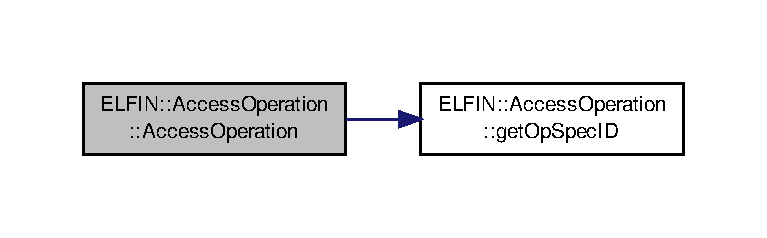
\includegraphics[width=350pt]{class_e_l_f_i_n_1_1_access_operation_ac2138a56bbd039b4d5c2354ddda25992_cgraph}
\end{center}
\end{figure}




\subsection{Member Function Documentation}
\hypertarget{class_e_l_f_i_n_1_1_access_operation_a7f5fbbbd2e32941d87c0f296d9869dd4}{\index{E\-L\-F\-I\-N\-::\-Access\-Operation@{E\-L\-F\-I\-N\-::\-Access\-Operation}!compare\-A\-C\-Op\-Spec\-Result@{compare\-A\-C\-Op\-Spec\-Result}}
\index{compare\-A\-C\-Op\-Spec\-Result@{compare\-A\-C\-Op\-Spec\-Result}!ELFIN::AccessOperation@{E\-L\-F\-I\-N\-::\-Access\-Operation}}
\subsubsection[{compare\-A\-C\-Op\-Spec\-Result}]{\setlength{\rightskip}{0pt plus 5cm}int E\-L\-F\-I\-N\-::\-Access\-Operation\-::compare\-A\-C\-Op\-Spec\-Result (
\begin{DoxyParamCaption}
\item[{L\-L\-R\-P\-::\-C\-Access\-Command\-Op\-Spec\-Result $\ast$}]{p\-Result1, }
\item[{L\-L\-R\-P\-::\-C\-Access\-Command\-Op\-Spec\-Result $\ast$}]{p\-Result2}
\end{DoxyParamCaption}
)\hspace{0.3cm}{\ttfamily [static]}}}\label{class_e_l_f_i_n_1_1_access_operation_a7f5fbbbd2e32941d87c0f296d9869dd4}


Compare two C\-Access\-Command\-Op\-Spec\-Result. If they are identical, returns 0. If not, returns non-\/zero value. 



Definition at line 380 of file Access\-Operation.\-cpp.



Here is the caller graph for this function\-:
\nopagebreak
\begin{figure}[H]
\begin{center}
\leavevmode
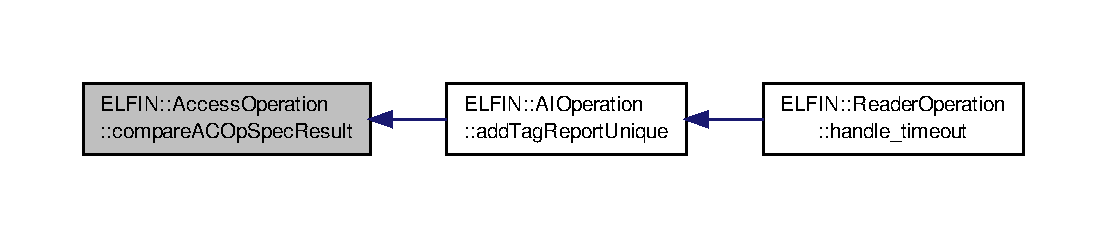
\includegraphics[width=350pt]{class_e_l_f_i_n_1_1_access_operation_a7f5fbbbd2e32941d87c0f296d9869dd4_icgraph}
\end{center}
\end{figure}


\hypertarget{class_e_l_f_i_n_1_1_access_operation_a7b21dfebb3248fe9e4105c8dca4ce897}{\index{E\-L\-F\-I\-N\-::\-Access\-Operation@{E\-L\-F\-I\-N\-::\-Access\-Operation}!execute\-Op\-Specs@{execute\-Op\-Specs}}
\index{execute\-Op\-Specs@{execute\-Op\-Specs}!ELFIN::AccessOperation@{E\-L\-F\-I\-N\-::\-Access\-Operation}}
\subsubsection[{execute\-Op\-Specs}]{\setlength{\rightskip}{0pt plus 5cm}int E\-L\-F\-I\-N\-::\-Access\-Operation\-::execute\-Op\-Specs (
\begin{DoxyParamCaption}
\item[{{\bf Stub\-Tag} $\ast$}]{p\-Stub\-Tag, }
\item[{L\-L\-R\-P\-::\-C\-Tag\-Report\-Data $\ast$}]{p\-Tag\-Report}
\end{DoxyParamCaption}
)}}\label{class_e_l_f_i_n_1_1_access_operation_a7b21dfebb3248fe9e4105c8dca4ce897}


Apply Op\-Spec to the provided \hyperlink{class_e_l_f_i_n_1_1_stub_tag}{Stub\-Tag}. The Op\-Spec\-Result would be stored to the p\-Tag\-Report object. 



Definition at line 182 of file Access\-Operation.\-cpp.



Here is the caller graph for this function\-:
\nopagebreak
\begin{figure}[H]
\begin{center}
\leavevmode
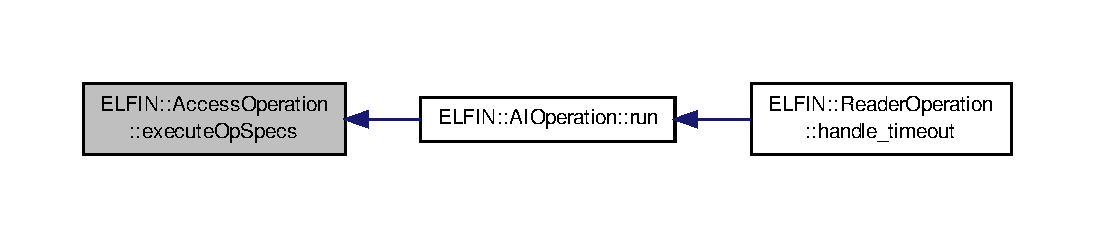
\includegraphics[width=350pt]{class_e_l_f_i_n_1_1_access_operation_a7b21dfebb3248fe9e4105c8dca4ce897_icgraph}
\end{center}
\end{figure}


\hypertarget{class_e_l_f_i_n_1_1_access_operation_a779c7cc8692989b0b1bc5789cef29e5b}{\index{E\-L\-F\-I\-N\-::\-Access\-Operation@{E\-L\-F\-I\-N\-::\-Access\-Operation}!get\-A\-C\-Op\-Spec\-Result\-O\-P\-Spec\-I\-D@{get\-A\-C\-Op\-Spec\-Result\-O\-P\-Spec\-I\-D}}
\index{get\-A\-C\-Op\-Spec\-Result\-O\-P\-Spec\-I\-D@{get\-A\-C\-Op\-Spec\-Result\-O\-P\-Spec\-I\-D}!ELFIN::AccessOperation@{E\-L\-F\-I\-N\-::\-Access\-Operation}}
\subsubsection[{get\-A\-C\-Op\-Spec\-Result\-O\-P\-Spec\-I\-D}]{\setlength{\rightskip}{0pt plus 5cm}L\-L\-R\-P\-::llrp\-\_\-u16\-\_\-t E\-L\-F\-I\-N\-::\-Access\-Operation\-::get\-A\-C\-Op\-Spec\-Result\-O\-P\-Spec\-I\-D (
\begin{DoxyParamCaption}
\item[{L\-L\-R\-P\-::\-C\-Access\-Command\-Op\-Spec\-Result $\ast$}]{p\-Access\-Command\-Op\-Spec\-Result}
\end{DoxyParamCaption}
)\hspace{0.3cm}{\ttfamily [static]}}}\label{class_e_l_f_i_n_1_1_access_operation_a779c7cc8692989b0b1bc5789cef29e5b}


Get the Op\-Spec id from the given Access\-Command\-Op\-Spec\-Result. 

\begin{DoxyRemark}{Remarks}
Because L\-L\-R\-P\-::\-C\-Access\-Command\-Op\-Spec\-Result type does not have method to get the Op\-Spec id, this method casts the Op\-Spec\-Result to its own type and return the Op\-Spec id. 
\end{DoxyRemark}


Definition at line 359 of file Access\-Operation.\-cpp.



Here is the caller graph for this function\-:
\nopagebreak
\begin{figure}[H]
\begin{center}
\leavevmode
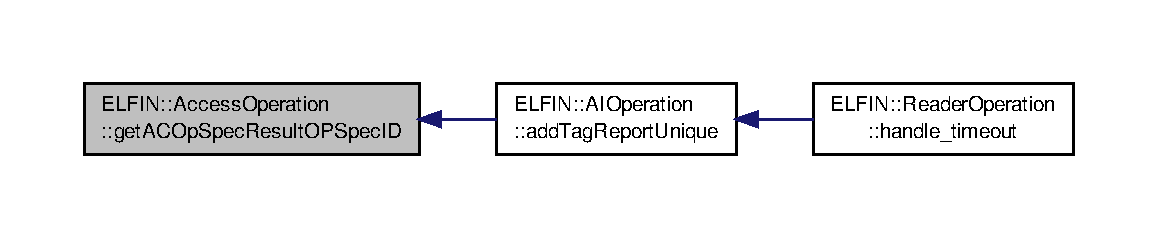
\includegraphics[width=350pt]{class_e_l_f_i_n_1_1_access_operation_a779c7cc8692989b0b1bc5789cef29e5b_icgraph}
\end{center}
\end{figure}


\hypertarget{class_e_l_f_i_n_1_1_access_operation_a153d7378aa347f667b22a2a170837622}{\index{E\-L\-F\-I\-N\-::\-Access\-Operation@{E\-L\-F\-I\-N\-::\-Access\-Operation}!get\-Op\-Spec\-I\-D@{get\-Op\-Spec\-I\-D}}
\index{get\-Op\-Spec\-I\-D@{get\-Op\-Spec\-I\-D}!ELFIN::AccessOperation@{E\-L\-F\-I\-N\-::\-Access\-Operation}}
\subsubsection[{get\-Op\-Spec\-I\-D}]{\setlength{\rightskip}{0pt plus 5cm}L\-L\-R\-P\-::llrp\-\_\-u16\-\_\-t E\-L\-F\-I\-N\-::\-Access\-Operation\-::get\-Op\-Spec\-I\-D (
\begin{DoxyParamCaption}
\item[{L\-L\-R\-P\-::\-C\-Access\-Command\-Op\-Spec $\ast$}]{p\-Op\-Spec}
\end{DoxyParamCaption}
)\hspace{0.3cm}{\ttfamily [static]}}}\label{class_e_l_f_i_n_1_1_access_operation_a153d7378aa347f667b22a2a170837622}


Get the Op\-Spec id from the given Op\-Spec. 

\begin{DoxyRemark}{Remarks}
Because L\-L\-R\-P\-::\-C\-Access\-Command\-Op\-Spec type does not have method to get the Op\-Spec id, this method casts the Op\-Spec to its own type and return the Op\-Spec id. 
\end{DoxyRemark}


Definition at line 62 of file Access\-Operation.\-cpp.



Here is the caller graph for this function\-:
\nopagebreak
\begin{figure}[H]
\begin{center}
\leavevmode
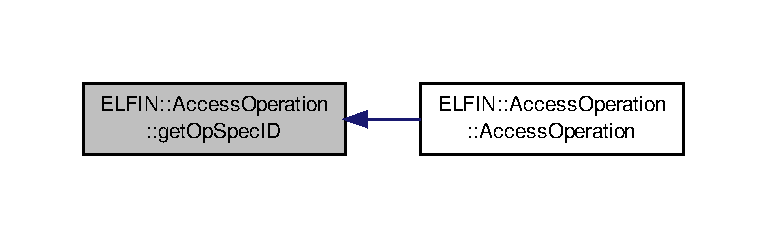
\includegraphics[width=350pt]{class_e_l_f_i_n_1_1_access_operation_a153d7378aa347f667b22a2a170837622_icgraph}
\end{center}
\end{figure}


\hypertarget{class_e_l_f_i_n_1_1_access_operation_aa7a89cb757c2d02c222a5a68703c3fd7}{\index{E\-L\-F\-I\-N\-::\-Access\-Operation@{E\-L\-F\-I\-N\-::\-Access\-Operation}!handle\-C1\-G2\-Block\-Erase@{handle\-C1\-G2\-Block\-Erase}}
\index{handle\-C1\-G2\-Block\-Erase@{handle\-C1\-G2\-Block\-Erase}!ELFIN::AccessOperation@{E\-L\-F\-I\-N\-::\-Access\-Operation}}
\subsubsection[{handle\-C1\-G2\-Block\-Erase}]{\setlength{\rightskip}{0pt plus 5cm}int E\-L\-F\-I\-N\-::\-Access\-Operation\-::handle\-C1\-G2\-Block\-Erase (
\begin{DoxyParamCaption}
\item[{L\-L\-R\-P\-::\-C\-Access\-Command\-Op\-Spec $\ast$}]{p\-Op\-Spec, }
\item[{{\bf Stub\-Tag} $\ast$}]{p\-Stub\-Tag, }
\item[{L\-L\-R\-P\-::\-C\-Tag\-Report\-Data $\ast$}]{p\-Tag\-Report}
\end{DoxyParamCaption}
)}}\label{class_e_l_f_i_n_1_1_access_operation_aa7a89cb757c2d02c222a5a68703c3fd7}


Handles corresponding Op\-Spec. But this method is not implemented yet. 



Definition at line 331 of file Access\-Operation.\-cpp.

\hypertarget{class_e_l_f_i_n_1_1_access_operation_a33d4d046de073308c854a5e16595197f}{\index{E\-L\-F\-I\-N\-::\-Access\-Operation@{E\-L\-F\-I\-N\-::\-Access\-Operation}!handle\-C1\-G2\-Block\-Write@{handle\-C1\-G2\-Block\-Write}}
\index{handle\-C1\-G2\-Block\-Write@{handle\-C1\-G2\-Block\-Write}!ELFIN::AccessOperation@{E\-L\-F\-I\-N\-::\-Access\-Operation}}
\subsubsection[{handle\-C1\-G2\-Block\-Write}]{\setlength{\rightskip}{0pt plus 5cm}int E\-L\-F\-I\-N\-::\-Access\-Operation\-::handle\-C1\-G2\-Block\-Write (
\begin{DoxyParamCaption}
\item[{L\-L\-R\-P\-::\-C\-Access\-Command\-Op\-Spec $\ast$}]{p\-Op\-Spec, }
\item[{{\bf Stub\-Tag} $\ast$}]{p\-Stub\-Tag, }
\item[{L\-L\-R\-P\-::\-C\-Tag\-Report\-Data $\ast$}]{p\-Tag\-Report}
\end{DoxyParamCaption}
)}}\label{class_e_l_f_i_n_1_1_access_operation_a33d4d046de073308c854a5e16595197f}


Handles corresponding Op\-Spec. But this method is not implemented yet. 



Definition at line 341 of file Access\-Operation.\-cpp.

\hypertarget{class_e_l_f_i_n_1_1_access_operation_aaa62c42a3e98fdb8a583a16561c4d416}{\index{E\-L\-F\-I\-N\-::\-Access\-Operation@{E\-L\-F\-I\-N\-::\-Access\-Operation}!handle\-C1\-G2\-Kill@{handle\-C1\-G2\-Kill}}
\index{handle\-C1\-G2\-Kill@{handle\-C1\-G2\-Kill}!ELFIN::AccessOperation@{E\-L\-F\-I\-N\-::\-Access\-Operation}}
\subsubsection[{handle\-C1\-G2\-Kill}]{\setlength{\rightskip}{0pt plus 5cm}int E\-L\-F\-I\-N\-::\-Access\-Operation\-::handle\-C1\-G2\-Kill (
\begin{DoxyParamCaption}
\item[{L\-L\-R\-P\-::\-C\-Access\-Command\-Op\-Spec $\ast$}]{p\-Op\-Spec, }
\item[{{\bf Stub\-Tag} $\ast$}]{p\-Stub\-Tag, }
\item[{L\-L\-R\-P\-::\-C\-Tag\-Report\-Data $\ast$}]{p\-Tag\-Report}
\end{DoxyParamCaption}
)}}\label{class_e_l_f_i_n_1_1_access_operation_aaa62c42a3e98fdb8a583a16561c4d416}


Handles corresponding Op\-Spec. But this method is not implemented yet. 



Definition at line 311 of file Access\-Operation.\-cpp.

\hypertarget{class_e_l_f_i_n_1_1_access_operation_a0fccaea52a98abc72788c6fe7b5bbe2d}{\index{E\-L\-F\-I\-N\-::\-Access\-Operation@{E\-L\-F\-I\-N\-::\-Access\-Operation}!handle\-C1\-G2\-Lock@{handle\-C1\-G2\-Lock}}
\index{handle\-C1\-G2\-Lock@{handle\-C1\-G2\-Lock}!ELFIN::AccessOperation@{E\-L\-F\-I\-N\-::\-Access\-Operation}}
\subsubsection[{handle\-C1\-G2\-Lock}]{\setlength{\rightskip}{0pt plus 5cm}int E\-L\-F\-I\-N\-::\-Access\-Operation\-::handle\-C1\-G2\-Lock (
\begin{DoxyParamCaption}
\item[{L\-L\-R\-P\-::\-C\-Access\-Command\-Op\-Spec $\ast$}]{p\-Op\-Spec, }
\item[{{\bf Stub\-Tag} $\ast$}]{p\-Stub\-Tag, }
\item[{L\-L\-R\-P\-::\-C\-Tag\-Report\-Data $\ast$}]{p\-Tag\-Report}
\end{DoxyParamCaption}
)}}\label{class_e_l_f_i_n_1_1_access_operation_a0fccaea52a98abc72788c6fe7b5bbe2d}


Handles corresponding Op\-Spec. But this method is not implemented yet. 



Definition at line 321 of file Access\-Operation.\-cpp.

\hypertarget{class_e_l_f_i_n_1_1_access_operation_af944ff98cc959755f16f892ef1be7559}{\index{E\-L\-F\-I\-N\-::\-Access\-Operation@{E\-L\-F\-I\-N\-::\-Access\-Operation}!handle\-C1\-G2\-Read@{handle\-C1\-G2\-Read}}
\index{handle\-C1\-G2\-Read@{handle\-C1\-G2\-Read}!ELFIN::AccessOperation@{E\-L\-F\-I\-N\-::\-Access\-Operation}}
\subsubsection[{handle\-C1\-G2\-Read}]{\setlength{\rightskip}{0pt plus 5cm}int E\-L\-F\-I\-N\-::\-Access\-Operation\-::handle\-C1\-G2\-Read (
\begin{DoxyParamCaption}
\item[{L\-L\-R\-P\-::\-C\-Access\-Command\-Op\-Spec $\ast$}]{p\-Op\-Spec, }
\item[{{\bf Stub\-Tag} $\ast$}]{p\-Stub\-Tag, }
\item[{L\-L\-R\-P\-::\-C\-Tag\-Report\-Data $\ast$}]{p\-Tag\-Report}
\end{DoxyParamCaption}
)}}\label{class_e_l_f_i_n_1_1_access_operation_af944ff98cc959755f16f892ef1be7559}


Handles C1\-G2\-Read Op\-Spec. The result is stored to the p\-Tag\-Report object. 



Definition at line 213 of file Access\-Operation.\-cpp.

\hypertarget{class_e_l_f_i_n_1_1_access_operation_a019256d2d181eec3688845227ed50a62}{\index{E\-L\-F\-I\-N\-::\-Access\-Operation@{E\-L\-F\-I\-N\-::\-Access\-Operation}!handle\-C1\-G2\-Write@{handle\-C1\-G2\-Write}}
\index{handle\-C1\-G2\-Write@{handle\-C1\-G2\-Write}!ELFIN::AccessOperation@{E\-L\-F\-I\-N\-::\-Access\-Operation}}
\subsubsection[{handle\-C1\-G2\-Write}]{\setlength{\rightskip}{0pt plus 5cm}int E\-L\-F\-I\-N\-::\-Access\-Operation\-::handle\-C1\-G2\-Write (
\begin{DoxyParamCaption}
\item[{L\-L\-R\-P\-::\-C\-Access\-Command\-Op\-Spec $\ast$}]{p\-Op\-Spec, }
\item[{{\bf Stub\-Tag} $\ast$}]{p\-Stub\-Tag, }
\item[{L\-L\-R\-P\-::\-C\-Tag\-Report\-Data $\ast$}]{p\-Tag\-Report}
\end{DoxyParamCaption}
)}}\label{class_e_l_f_i_n_1_1_access_operation_a019256d2d181eec3688845227ed50a62}


Handles C1\-G2\-Write Op\-Spec. The result is stored to the p\-Tag\-Report object. 



Definition at line 268 of file Access\-Operation.\-cpp.

\hypertarget{class_e_l_f_i_n_1_1_access_operation_abd6ee0b2cb143103440bd9caed9dff19}{\index{E\-L\-F\-I\-N\-::\-Access\-Operation@{E\-L\-F\-I\-N\-::\-Access\-Operation}!is\-Valid@{is\-Valid}}
\index{is\-Valid@{is\-Valid}!ELFIN::AccessOperation@{E\-L\-F\-I\-N\-::\-Access\-Operation}}
\subsubsection[{is\-Valid}]{\setlength{\rightskip}{0pt plus 5cm}int E\-L\-F\-I\-N\-::\-Access\-Operation\-::is\-Valid (
\begin{DoxyParamCaption}
{}
\end{DoxyParamCaption}
)}}\label{class_e_l_f_i_n_1_1_access_operation_abd6ee0b2cb143103440bd9caed9dff19}


Check the validity of \hyperlink{class_e_l_f_i_n_1_1_access_operation}{Access\-Operation} object. 



Definition at line 351 of file Access\-Operation.\-cpp.

\hypertarget{class_e_l_f_i_n_1_1_access_operation_a9f928363dd0ab1a6a0ef2f3e594e60a4}{\index{E\-L\-F\-I\-N\-::\-Access\-Operation@{E\-L\-F\-I\-N\-::\-Access\-Operation}!match\-Tag\-Spec@{match\-Tag\-Spec}}
\index{match\-Tag\-Spec@{match\-Tag\-Spec}!ELFIN::AccessOperation@{E\-L\-F\-I\-N\-::\-Access\-Operation}}
\subsubsection[{match\-Tag\-Spec}]{\setlength{\rightskip}{0pt plus 5cm}int E\-L\-F\-I\-N\-::\-Access\-Operation\-::match\-Tag\-Spec (
\begin{DoxyParamCaption}
\item[{{\bf Stub\-Tag} $\ast$}]{p\-Stub\-Tag, }
\item[{L\-L\-R\-P\-::llrp\-\_\-u32\-\_\-t}]{p\-R\-O\-Spec\-I\-D}
\end{DoxyParamCaption}
)}}\label{class_e_l_f_i_n_1_1_access_operation_a9f928363dd0ab1a6a0ef2f3e594e60a4}


Match the provided \hyperlink{class_e_l_f_i_n_1_1_stub_tag}{Stub\-Tag} and R\-O\-Spec\-I\-D to the current C1\-G2\-Target\-Tag. 

\begin{DoxyRefDesc}{Todo}
\item[\hyperlink{todo__todo000002}{Todo}]need to remove redundant code \end{DoxyRefDesc}


\begin{DoxyRefDesc}{Todo}
\item[\hyperlink{todo__todo000003}{Todo}]Need to modify not only support the pointer multiple of 8, but also other values \end{DoxyRefDesc}


\begin{DoxyRefDesc}{Todo}
\item[\hyperlink{todo__todo000004}{Todo}]Optimize this, by not reading whole mb contents, but just target area. \end{DoxyRefDesc}


\begin{DoxyRefDesc}{Todo}
\item[\hyperlink{todo__todo000005}{Todo}]Need to modify not only support the pointer multiple of 8, but also other values \end{DoxyRefDesc}


Definition at line 92 of file Access\-Operation.\-cpp.



Here is the caller graph for this function\-:
\nopagebreak
\begin{figure}[H]
\begin{center}
\leavevmode
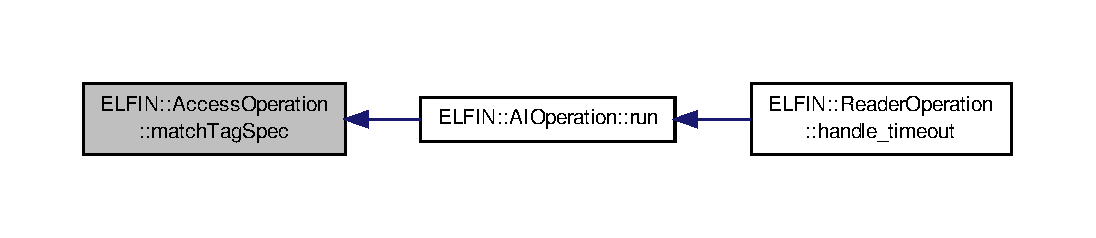
\includegraphics[width=350pt]{class_e_l_f_i_n_1_1_access_operation_a9f928363dd0ab1a6a0ef2f3e594e60a4_icgraph}
\end{center}
\end{figure}




\subsection{Member Data Documentation}
\hypertarget{class_e_l_f_i_n_1_1_access_operation_ac62e4350f2fa25abff5ffa61ac853a90}{\index{E\-L\-F\-I\-N\-::\-Access\-Operation@{E\-L\-F\-I\-N\-::\-Access\-Operation}!\-\_\-p\-Op\-Spec\-Map@{\-\_\-p\-Op\-Spec\-Map}}
\index{\-\_\-p\-Op\-Spec\-Map@{\-\_\-p\-Op\-Spec\-Map}!ELFIN::AccessOperation@{E\-L\-F\-I\-N\-::\-Access\-Operation}}
\subsubsection[{\-\_\-p\-Op\-Spec\-Map}]{\setlength{\rightskip}{0pt plus 5cm}O\-P\-Specs\-Map E\-L\-F\-I\-N\-::\-Access\-Operation\-::\-\_\-p\-Op\-Spec\-Map\hspace{0.3cm}{\ttfamily [private]}}}\label{class_e_l_f_i_n_1_1_access_operation_ac62e4350f2fa25abff5ffa61ac853a90}


C\-Access\-Command\-Op\-Spec container. 



Definition at line 66 of file Access\-Operation.\-h.



The documentation for this class was generated from the following files\-:\begin{DoxyCompactItemize}
\item 
elfin\-\_\-src/\hyperlink{_access_operation_8h}{Access\-Operation.\-h}\item 
elfin\-\_\-src/\hyperlink{_access_operation_8cpp}{Access\-Operation.\-cpp}\end{DoxyCompactItemize}

\hypertarget{class_e_l_f_i_n_1_1_a_i_operation}{\section{E\-L\-F\-I\-N\-:\-:A\-I\-Operation Class Reference}
\label{class_e_l_f_i_n_1_1_a_i_operation}\index{E\-L\-F\-I\-N\-::\-A\-I\-Operation@{E\-L\-F\-I\-N\-::\-A\-I\-Operation}}
}


A single antenna inventory operation generated based on the A\-I\-Spec parameter in the given R\-O\-Spec.  




{\ttfamily \#include $<$A\-I\-Operation.\-h$>$}



Inheritance diagram for E\-L\-F\-I\-N\-:\-:A\-I\-Operation\-:
\nopagebreak
\begin{figure}[H]
\begin{center}
\leavevmode
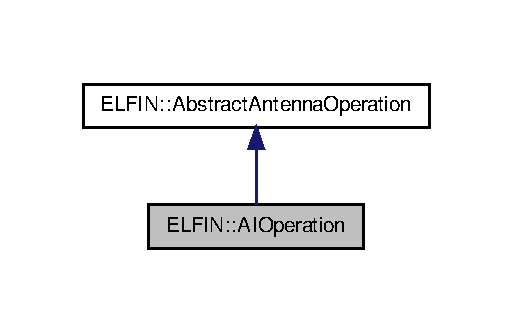
\includegraphics[width=246pt]{class_e_l_f_i_n_1_1_a_i_operation__inherit__graph}
\end{center}
\end{figure}


Collaboration diagram for E\-L\-F\-I\-N\-:\-:A\-I\-Operation\-:
\nopagebreak
\begin{figure}[H]
\begin{center}
\leavevmode
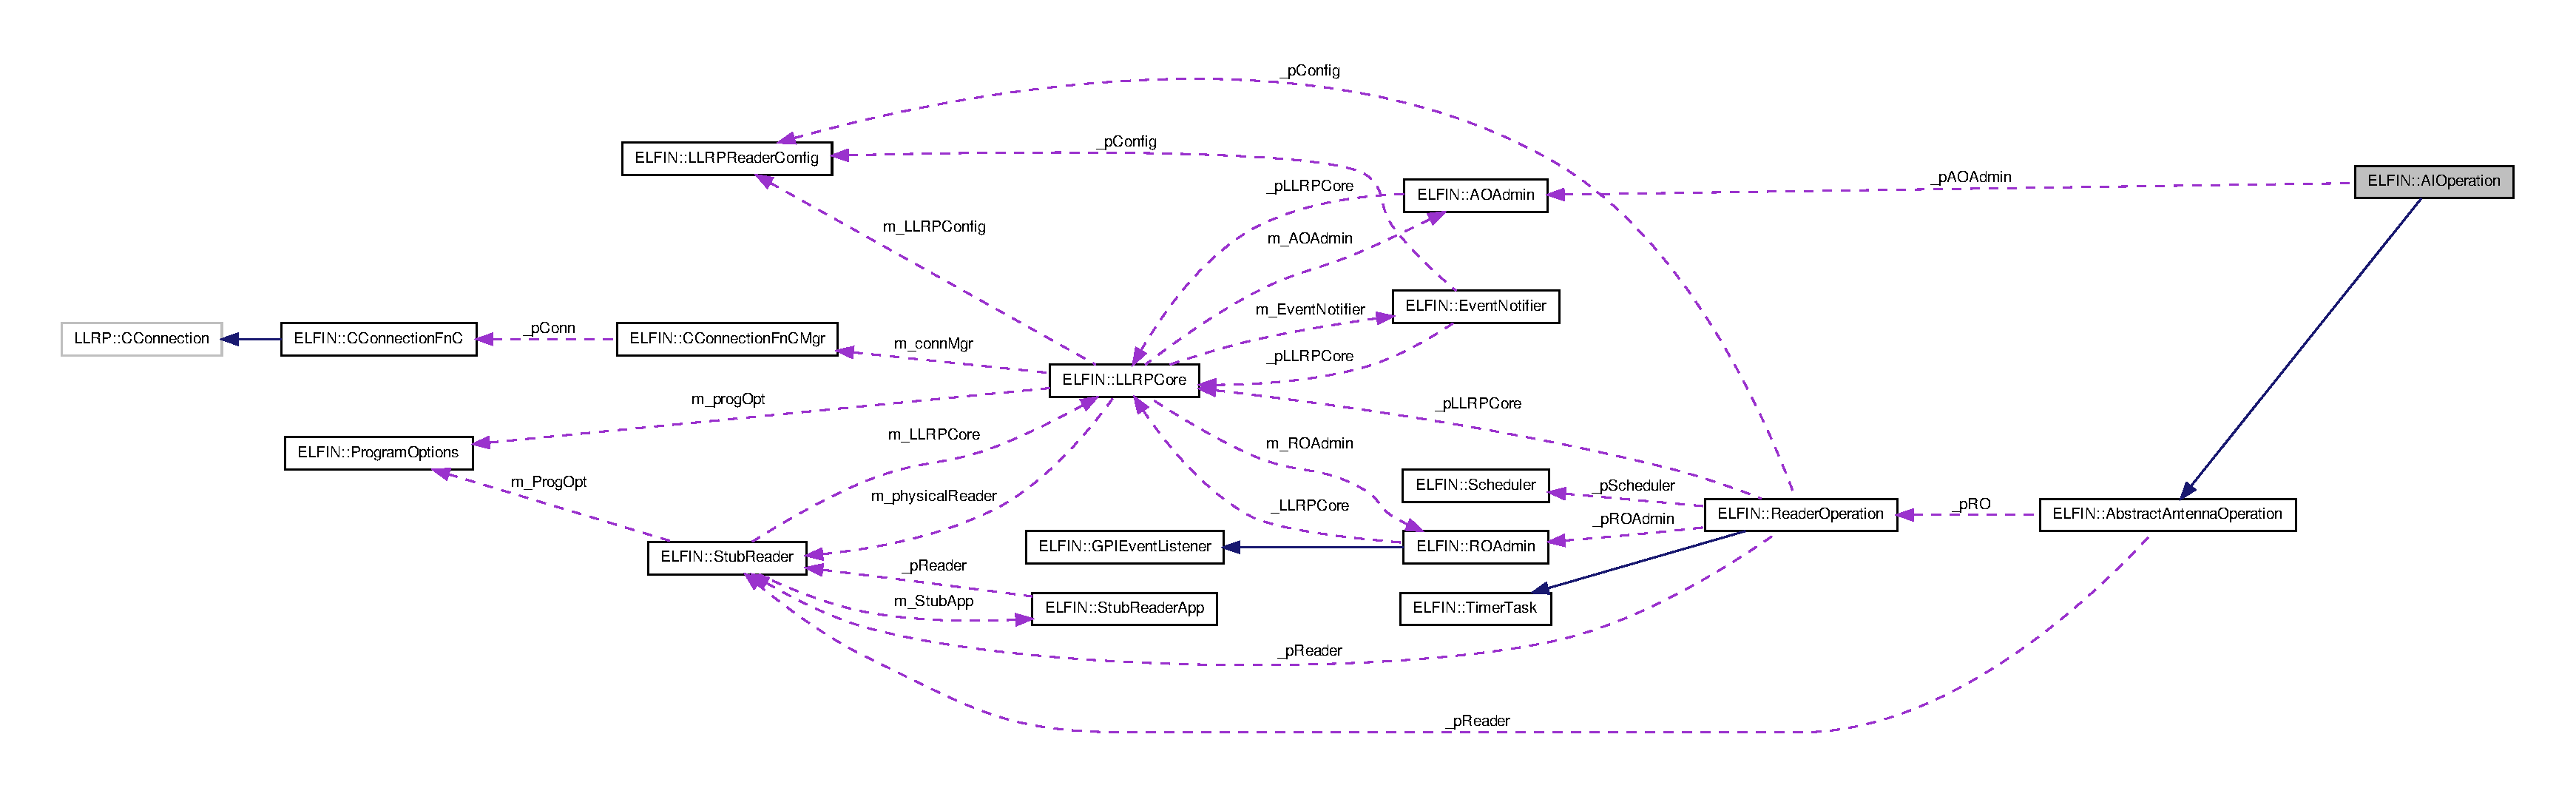
\includegraphics[width=350pt]{class_e_l_f_i_n_1_1_a_i_operation__coll__graph}
\end{center}
\end{figure}
\subsection*{Public Member Functions}
\begin{DoxyCompactItemize}
\item 
\hyperlink{class_e_l_f_i_n_1_1_a_i_operation_a77f1def7da7b7712981030a08746513e}{A\-I\-Operation} (L\-L\-R\-P\-::\-C\-R\-O\-Spec $\ast$\-\_\-\-\_\-p\-R\-O\-Spec, L\-L\-R\-P\-::\-C\-A\-I\-Spec $\ast$\-\_\-\-\_\-p\-A\-I\-Spec, \hyperlink{class_e_l_f_i_n_1_1_stub_reader}{Stub\-Reader} $\ast$\-\_\-\-\_\-p\-Reader, \hyperlink{class_e_l_f_i_n_1_1_reader_operation}{Reader\-Operation} $\ast$\-\_\-\-\_\-p\-R\-O, \hyperlink{class_e_l_f_i_n_1_1_a_o_admin}{A\-O\-Admin} $\ast$\-\_\-\-\_\-p\-A\-O\-Admin, int \-\_\-\-\_\-p\-Spec\-Index)
\begin{DoxyCompactList}\small\item\em Constructor of \hyperlink{class_e_l_f_i_n_1_1_a_i_operation}{A\-I\-Operation} class. \end{DoxyCompactList}\item 
\hyperlink{class_e_l_f_i_n_1_1_a_i_operation_a95756463bda120c3ce5290f5dffc9747}{$\sim$\-A\-I\-Operation} ()
\begin{DoxyCompactList}\small\item\em Destructor of \hyperlink{class_e_l_f_i_n_1_1_a_i_operation}{A\-I\-Operation} class. \end{DoxyCompactList}\item 
Tag\-Report\-Set $\ast$ \hyperlink{class_e_l_f_i_n_1_1_a_i_operation_a13259c8516e1b5fb465e553c4c5dae01}{run} ()
\begin{DoxyCompactList}\small\item\em Run the \hyperlink{class_e_l_f_i_n_1_1_a_i_operation}{A\-I\-Operation} according to the C\-A\-I\-Spec. \end{DoxyCompactList}\end{DoxyCompactItemize}
\subsection*{Static Public Member Functions}
\begin{DoxyCompactItemize}
\item 
static int \hyperlink{class_e_l_f_i_n_1_1_a_i_operation_ac37fc39b75785f9188b02cb62988dd18}{add\-Tag\-Report\-Unique} (Tag\-Report\-Set $\ast$p\-Set, L\-L\-R\-P\-::\-C\-Tag\-Report\-Data $\ast$p\-Rpt)
\begin{DoxyCompactList}\small\item\em Add the given p\-Rpt to the p\-Set. If the same E\-P\-C number exists in the vector, then overwrite it. \end{DoxyCompactList}\end{DoxyCompactItemize}
\subsection*{Private Member Functions}
\begin{DoxyCompactItemize}
\item 
L\-L\-R\-P\-::\-C\-Tag\-Report\-Data $\ast$ \hyperlink{class_e_l_f_i_n_1_1_a_i_operation_ab691057f5895c3af2dc617f2fcf4d9c4}{create\-Tag\-Report\-Data} (\hyperlink{class_e_l_f_i_n_1_1_stub_tag}{Stub\-Tag} $\ast$p\-Stub\-Tag, int p\-Inv\-Spec\-I\-D)
\begin{DoxyCompactList}\small\item\em Create base tag report data for the given \hyperlink{class_e_l_f_i_n_1_1_stub_tag}{Stub\-Tag}. \end{DoxyCompactList}\item 
void \hyperlink{class_e_l_f_i_n_1_1_a_i_operation_a8cc8f6baacabcddac43853a5f72fa580}{run\-\_\-\-A\-I\-Spec\-Stop\-Trigger\-Thread} (int stop\-M\-S)
\begin{DoxyCompactList}\small\item\em This method is used to make thread for stop trigger which is related to time. After given time, interrupts tag singulation. \end{DoxyCompactList}\end{DoxyCompactItemize}
\subsection*{Private Attributes}
\begin{DoxyCompactItemize}
\item 
\hypertarget{class_e_l_f_i_n_1_1_a_i_operation_a93b754086e1bc532db5b22d0c8d785f1}{L\-L\-R\-P\-::\-C\-R\-O\-Spec $\ast$ {\bfseries \-\_\-p\-R\-O\-Spec}}\label{class_e_l_f_i_n_1_1_a_i_operation_a93b754086e1bc532db5b22d0c8d785f1}

\item 
\hypertarget{class_e_l_f_i_n_1_1_a_i_operation_a08a5b54d1283d2c54686f9a4f82fea29}{L\-L\-R\-P\-::\-C\-A\-I\-Spec $\ast$ {\bfseries \-\_\-p\-A\-I\-Spec}}\label{class_e_l_f_i_n_1_1_a_i_operation_a08a5b54d1283d2c54686f9a4f82fea29}

\item 
\hypertarget{class_e_l_f_i_n_1_1_a_i_operation_a79732664a72ca6ed9fbcff3cb0c65a03}{L\-L\-R\-P\-::\-C\-R\-O\-Report\-Spec $\ast$ {\bfseries \-\_\-p\-R\-O\-Report\-Spec}}\label{class_e_l_f_i_n_1_1_a_i_operation_a79732664a72ca6ed9fbcff3cb0c65a03}

\item 
\hypertarget{class_e_l_f_i_n_1_1_a_i_operation_a2c4e4215a3a81717b30386f6d3bcd2cf}{L\-L\-R\-P\-::\-C\-C1\-G2\-E\-P\-C\-Memory\-Selector $\ast$ {\bfseries \-\_\-p\-Mem\-Selector}}\label{class_e_l_f_i_n_1_1_a_i_operation_a2c4e4215a3a81717b30386f6d3bcd2cf}

\item 
Tag\-Report\-Set $\ast$ \hyperlink{class_e_l_f_i_n_1_1_a_i_operation_a565a8b3215c53586eaaf56a91e62a4bd}{\-\_\-p\-Tag\-Report\-Set}
\begin{DoxyCompactList}\small\item\em C\-Tag\-Report\-Data container. \end{DoxyCompactList}\item 
\hypertarget{class_e_l_f_i_n_1_1_a_i_operation_a7c6ce0591568c71473935b6191603eae}{boost\-::thread {\bfseries \-\_\-p\-A\-I\-Spec\-Stop\-Trigger\-Thread}}\label{class_e_l_f_i_n_1_1_a_i_operation_a7c6ce0591568c71473935b6191603eae}

\item 
\hypertarget{class_e_l_f_i_n_1_1_a_i_operation_ae45f89acd8dd62e448a96772137a9678}{int {\bfseries is\-On\-Singulation}}\label{class_e_l_f_i_n_1_1_a_i_operation_ae45f89acd8dd62e448a96772137a9678}

\item 
\hypertarget{class_e_l_f_i_n_1_1_a_i_operation_a5a2d4fa187eafd1a1256a9c8df096a40}{\hyperlink{class_e_l_f_i_n_1_1_a_o_admin}{A\-O\-Admin} $\ast$ {\bfseries \-\_\-p\-A\-O\-Admin}}\label{class_e_l_f_i_n_1_1_a_i_operation_a5a2d4fa187eafd1a1256a9c8df096a40}

\end{DoxyCompactItemize}
\subsection*{Additional Inherited Members}


\subsection{Detailed Description}
A single antenna inventory operation generated based on the A\-I\-Spec parameter in the given R\-O\-Spec. 

Definition at line 23 of file A\-I\-Operation.\-h.



\subsection{Constructor \& Destructor Documentation}
\hypertarget{class_e_l_f_i_n_1_1_a_i_operation_a77f1def7da7b7712981030a08746513e}{\index{E\-L\-F\-I\-N\-::\-A\-I\-Operation@{E\-L\-F\-I\-N\-::\-A\-I\-Operation}!A\-I\-Operation@{A\-I\-Operation}}
\index{A\-I\-Operation@{A\-I\-Operation}!ELFIN::AIOperation@{E\-L\-F\-I\-N\-::\-A\-I\-Operation}}
\subsubsection[{A\-I\-Operation}]{\setlength{\rightskip}{0pt plus 5cm}E\-L\-F\-I\-N\-::\-A\-I\-Operation\-::\-A\-I\-Operation (
\begin{DoxyParamCaption}
\item[{L\-L\-R\-P\-::\-C\-R\-O\-Spec $\ast$}]{\-\_\-\-\_\-p\-R\-O\-Spec, }
\item[{L\-L\-R\-P\-::\-C\-A\-I\-Spec $\ast$}]{\-\_\-\-\_\-p\-A\-I\-Spec, }
\item[{{\bf Stub\-Reader} $\ast$}]{\-\_\-\-\_\-p\-Reader, }
\item[{{\bf Reader\-Operation} $\ast$}]{\-\_\-\-\_\-p\-R\-O, }
\item[{{\bf A\-O\-Admin} $\ast$}]{\-\_\-\-\_\-p\-A\-O\-Admin, }
\item[{int}]{\-\_\-\-\_\-p\-Spec\-Index}
\end{DoxyParamCaption}
)}}\label{class_e_l_f_i_n_1_1_a_i_operation_a77f1def7da7b7712981030a08746513e}


Constructor of \hyperlink{class_e_l_f_i_n_1_1_a_i_operation}{A\-I\-Operation} class. 



Definition at line 15 of file A\-I\-Operation.\-cpp.

\hypertarget{class_e_l_f_i_n_1_1_a_i_operation_a95756463bda120c3ce5290f5dffc9747}{\index{E\-L\-F\-I\-N\-::\-A\-I\-Operation@{E\-L\-F\-I\-N\-::\-A\-I\-Operation}!$\sim$\-A\-I\-Operation@{$\sim$\-A\-I\-Operation}}
\index{$\sim$\-A\-I\-Operation@{$\sim$\-A\-I\-Operation}!ELFIN::AIOperation@{E\-L\-F\-I\-N\-::\-A\-I\-Operation}}
\subsubsection[{$\sim$\-A\-I\-Operation}]{\setlength{\rightskip}{0pt plus 5cm}E\-L\-F\-I\-N\-::\-A\-I\-Operation\-::$\sim$\-A\-I\-Operation (
\begin{DoxyParamCaption}
{}
\end{DoxyParamCaption}
)}}\label{class_e_l_f_i_n_1_1_a_i_operation_a95756463bda120c3ce5290f5dffc9747}


Destructor of \hyperlink{class_e_l_f_i_n_1_1_a_i_operation}{A\-I\-Operation} class. 



Definition at line 37 of file A\-I\-Operation.\-cpp.



\subsection{Member Function Documentation}
\hypertarget{class_e_l_f_i_n_1_1_a_i_operation_ac37fc39b75785f9188b02cb62988dd18}{\index{E\-L\-F\-I\-N\-::\-A\-I\-Operation@{E\-L\-F\-I\-N\-::\-A\-I\-Operation}!add\-Tag\-Report\-Unique@{add\-Tag\-Report\-Unique}}
\index{add\-Tag\-Report\-Unique@{add\-Tag\-Report\-Unique}!ELFIN::AIOperation@{E\-L\-F\-I\-N\-::\-A\-I\-Operation}}
\subsubsection[{add\-Tag\-Report\-Unique}]{\setlength{\rightskip}{0pt plus 5cm}int E\-L\-F\-I\-N\-::\-A\-I\-Operation\-::add\-Tag\-Report\-Unique (
\begin{DoxyParamCaption}
\item[{Tag\-Report\-Set $\ast$}]{p\-Set, }
\item[{L\-L\-R\-P\-::\-C\-Tag\-Report\-Data $\ast$}]{p\-Rpt}
\end{DoxyParamCaption}
)\hspace{0.3cm}{\ttfamily [static]}}}\label{class_e_l_f_i_n_1_1_a_i_operation_ac37fc39b75785f9188b02cb62988dd18}


Add the given p\-Rpt to the p\-Set. If the same E\-P\-C number exists in the vector, then overwrite it. 



Definition at line 399 of file A\-I\-Operation.\-cpp.



Here is the call graph for this function\-:
\nopagebreak
\begin{figure}[H]
\begin{center}
\leavevmode
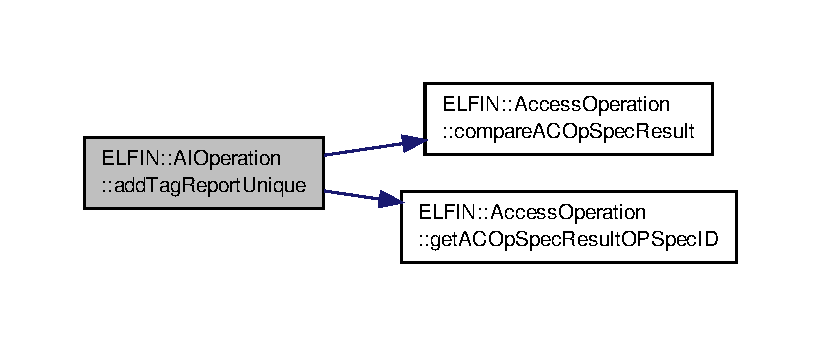
\includegraphics[width=350pt]{class_e_l_f_i_n_1_1_a_i_operation_ac37fc39b75785f9188b02cb62988dd18_cgraph}
\end{center}
\end{figure}




Here is the caller graph for this function\-:
\nopagebreak
\begin{figure}[H]
\begin{center}
\leavevmode
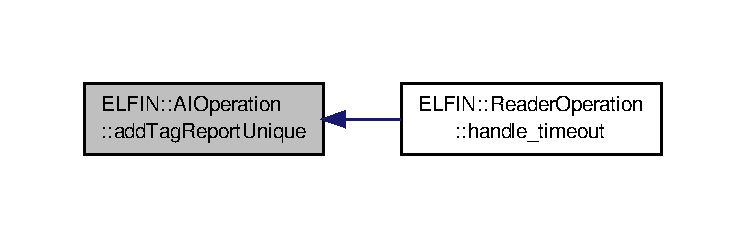
\includegraphics[width=350pt]{class_e_l_f_i_n_1_1_a_i_operation_ac37fc39b75785f9188b02cb62988dd18_icgraph}
\end{center}
\end{figure}


\hypertarget{class_e_l_f_i_n_1_1_a_i_operation_ab691057f5895c3af2dc617f2fcf4d9c4}{\index{E\-L\-F\-I\-N\-::\-A\-I\-Operation@{E\-L\-F\-I\-N\-::\-A\-I\-Operation}!create\-Tag\-Report\-Data@{create\-Tag\-Report\-Data}}
\index{create\-Tag\-Report\-Data@{create\-Tag\-Report\-Data}!ELFIN::AIOperation@{E\-L\-F\-I\-N\-::\-A\-I\-Operation}}
\subsubsection[{create\-Tag\-Report\-Data}]{\setlength{\rightskip}{0pt plus 5cm}L\-L\-R\-P\-::\-C\-Tag\-Report\-Data $\ast$ E\-L\-F\-I\-N\-::\-A\-I\-Operation\-::create\-Tag\-Report\-Data (
\begin{DoxyParamCaption}
\item[{{\bf Stub\-Tag} $\ast$}]{p\-Stub\-Tag, }
\item[{int}]{p\-Inv\-Spec\-I\-D}
\end{DoxyParamCaption}
)\hspace{0.3cm}{\ttfamily [private]}}}\label{class_e_l_f_i_n_1_1_a_i_operation_ab691057f5895c3af2dc617f2fcf4d9c4}


Create base tag report data for the given \hyperlink{class_e_l_f_i_n_1_1_stub_tag}{Stub\-Tag}. 



Definition at line 322 of file A\-I\-Operation.\-cpp.

\hypertarget{class_e_l_f_i_n_1_1_a_i_operation_a13259c8516e1b5fb465e553c4c5dae01}{\index{E\-L\-F\-I\-N\-::\-A\-I\-Operation@{E\-L\-F\-I\-N\-::\-A\-I\-Operation}!run@{run}}
\index{run@{run}!ELFIN::AIOperation@{E\-L\-F\-I\-N\-::\-A\-I\-Operation}}
\subsubsection[{run}]{\setlength{\rightskip}{0pt plus 5cm}E\-L\-F\-I\-N\-::\-Tag\-Report\-Set $\ast$ E\-L\-F\-I\-N\-::\-A\-I\-Operation\-::run (
\begin{DoxyParamCaption}
{}
\end{DoxyParamCaption}
)\hspace{0.3cm}{\ttfamily [virtual]}}}\label{class_e_l_f_i_n_1_1_a_i_operation_a13259c8516e1b5fb465e553c4c5dae01}


Run the \hyperlink{class_e_l_f_i_n_1_1_a_i_operation}{A\-I\-Operation} according to the C\-A\-I\-Spec. 

\begin{DoxyRefDesc}{Todo}
\item[\hyperlink{todo__todo000006}{Todo}]add G\-P\-I event listener \end{DoxyRefDesc}


\begin{DoxyRefDesc}{Todo}
\item[\hyperlink{todo__todo000007}{Todo}]Add handling of Antenna\-Configurations of Inventory\-Parameter\-Spec \end{DoxyRefDesc}


\begin{DoxyRefDesc}{Todo}
\item[\hyperlink{todo__todo000008}{Todo}]iterate Access\-Spec in the sequence of enable time, and execute only the firstly matched one. \end{DoxyRefDesc}


Implements \hyperlink{class_e_l_f_i_n_1_1_abstract_antenna_operation_af8cd8a5e57d157a3af20c28c6e573bfb}{E\-L\-F\-I\-N\-::\-Abstract\-Antenna\-Operation}.



Definition at line 43 of file A\-I\-Operation.\-cpp.



Here is the call graph for this function\-:
\nopagebreak
\begin{figure}[H]
\begin{center}
\leavevmode
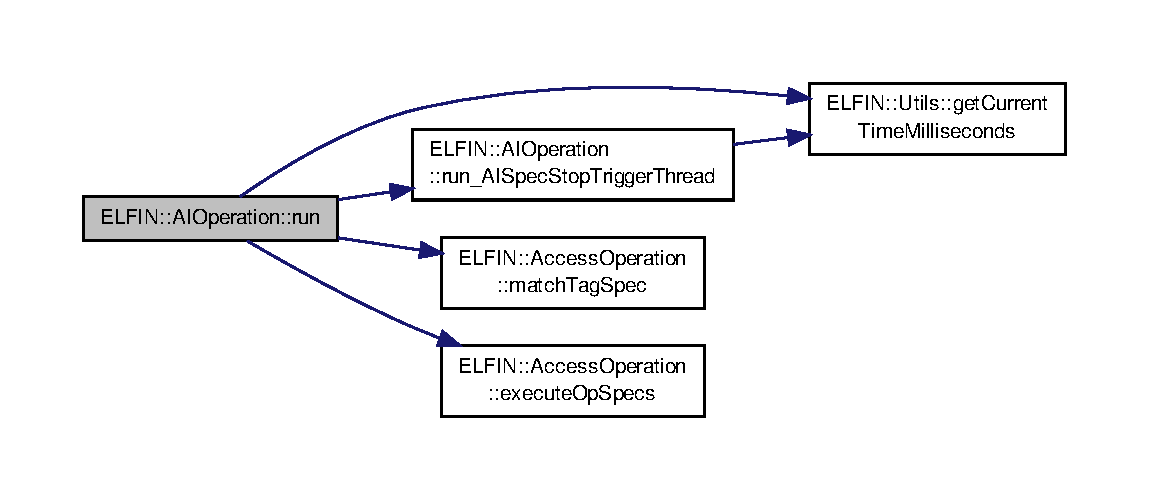
\includegraphics[width=350pt]{class_e_l_f_i_n_1_1_a_i_operation_a13259c8516e1b5fb465e553c4c5dae01_cgraph}
\end{center}
\end{figure}




Here is the caller graph for this function\-:
\nopagebreak
\begin{figure}[H]
\begin{center}
\leavevmode
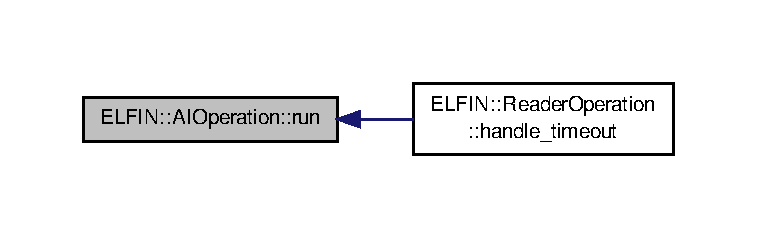
\includegraphics[width=350pt]{class_e_l_f_i_n_1_1_a_i_operation_a13259c8516e1b5fb465e553c4c5dae01_icgraph}
\end{center}
\end{figure}


\hypertarget{class_e_l_f_i_n_1_1_a_i_operation_a8cc8f6baacabcddac43853a5f72fa580}{\index{E\-L\-F\-I\-N\-::\-A\-I\-Operation@{E\-L\-F\-I\-N\-::\-A\-I\-Operation}!run\-\_\-\-A\-I\-Spec\-Stop\-Trigger\-Thread@{run\-\_\-\-A\-I\-Spec\-Stop\-Trigger\-Thread}}
\index{run\-\_\-\-A\-I\-Spec\-Stop\-Trigger\-Thread@{run\-\_\-\-A\-I\-Spec\-Stop\-Trigger\-Thread}!ELFIN::AIOperation@{E\-L\-F\-I\-N\-::\-A\-I\-Operation}}
\subsubsection[{run\-\_\-\-A\-I\-Spec\-Stop\-Trigger\-Thread}]{\setlength{\rightskip}{0pt plus 5cm}void E\-L\-F\-I\-N\-::\-A\-I\-Operation\-::run\-\_\-\-A\-I\-Spec\-Stop\-Trigger\-Thread (
\begin{DoxyParamCaption}
\item[{int}]{stop\-M\-S}
\end{DoxyParamCaption}
)\hspace{0.3cm}{\ttfamily [private]}}}\label{class_e_l_f_i_n_1_1_a_i_operation_a8cc8f6baacabcddac43853a5f72fa580}


This method is used to make thread for stop trigger which is related to time. After given time, interrupts tag singulation. 



Definition at line 458 of file A\-I\-Operation.\-cpp.



Here is the call graph for this function\-:
\nopagebreak
\begin{figure}[H]
\begin{center}
\leavevmode
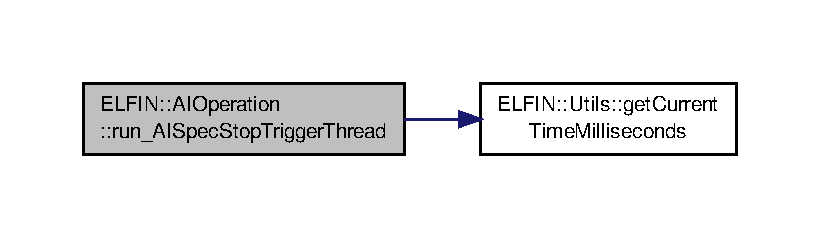
\includegraphics[width=350pt]{class_e_l_f_i_n_1_1_a_i_operation_a8cc8f6baacabcddac43853a5f72fa580_cgraph}
\end{center}
\end{figure}




Here is the caller graph for this function\-:
\nopagebreak
\begin{figure}[H]
\begin{center}
\leavevmode
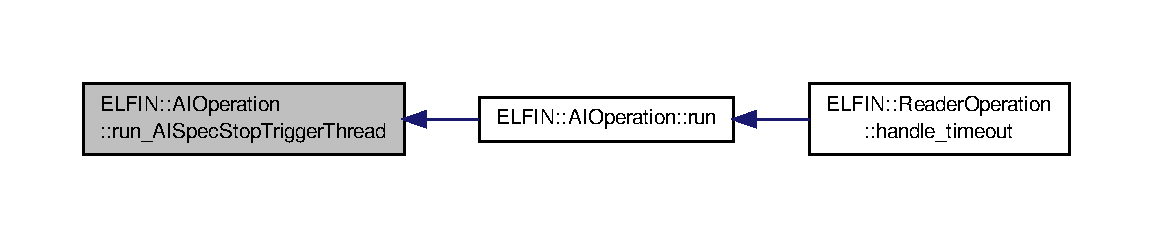
\includegraphics[width=350pt]{class_e_l_f_i_n_1_1_a_i_operation_a8cc8f6baacabcddac43853a5f72fa580_icgraph}
\end{center}
\end{figure}




\subsection{Member Data Documentation}
\hypertarget{class_e_l_f_i_n_1_1_a_i_operation_a565a8b3215c53586eaaf56a91e62a4bd}{\index{E\-L\-F\-I\-N\-::\-A\-I\-Operation@{E\-L\-F\-I\-N\-::\-A\-I\-Operation}!\-\_\-p\-Tag\-Report\-Set@{\-\_\-p\-Tag\-Report\-Set}}
\index{\-\_\-p\-Tag\-Report\-Set@{\-\_\-p\-Tag\-Report\-Set}!ELFIN::AIOperation@{E\-L\-F\-I\-N\-::\-A\-I\-Operation}}
\subsubsection[{\-\_\-p\-Tag\-Report\-Set}]{\setlength{\rightskip}{0pt plus 5cm}Tag\-Report\-Set$\ast$ E\-L\-F\-I\-N\-::\-A\-I\-Operation\-::\-\_\-p\-Tag\-Report\-Set\hspace{0.3cm}{\ttfamily [private]}}}\label{class_e_l_f_i_n_1_1_a_i_operation_a565a8b3215c53586eaaf56a91e62a4bd}


C\-Tag\-Report\-Data container. 



Definition at line 44 of file A\-I\-Operation.\-h.



The documentation for this class was generated from the following files\-:\begin{DoxyCompactItemize}
\item 
elfin\-\_\-src/\hyperlink{_a_i_operation_8h}{A\-I\-Operation.\-h}\item 
elfin\-\_\-src/\hyperlink{_a_i_operation_8cpp}{A\-I\-Operation.\-cpp}\end{DoxyCompactItemize}

\hypertarget{struct_e_l_f_i_n_1_1_sample_reader_1_1antenna}{\section{E\-L\-F\-I\-N\-:\-:Sample\-Reader\-:\-:antenna Struct Reference}
\label{struct_e_l_f_i_n_1_1_sample_reader_1_1antenna}\index{E\-L\-F\-I\-N\-::\-Sample\-Reader\-::antenna@{E\-L\-F\-I\-N\-::\-Sample\-Reader\-::antenna}}
}


Collaboration diagram for E\-L\-F\-I\-N\-:\-:Sample\-Reader\-:\-:antenna\-:
\nopagebreak
\begin{figure}[H]
\begin{center}
\leavevmode
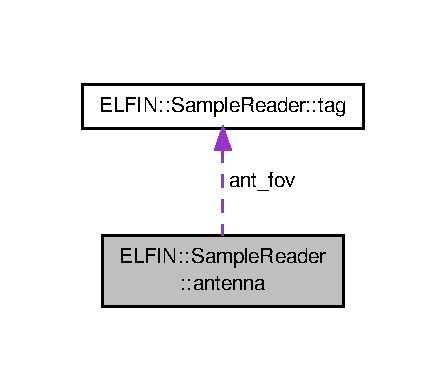
\includegraphics[width=214pt]{struct_e_l_f_i_n_1_1_sample_reader_1_1antenna__coll__graph}
\end{center}
\end{figure}
\subsection*{Public Attributes}
\begin{DoxyCompactItemize}
\item 
\hypertarget{struct_e_l_f_i_n_1_1_sample_reader_1_1antenna_a427c5e78cd9571cbaeedd39b42cb2bf1}{int {\bfseries ant\-\_\-id}}\label{struct_e_l_f_i_n_1_1_sample_reader_1_1antenna_a427c5e78cd9571cbaeedd39b42cb2bf1}

\item 
\hypertarget{struct_e_l_f_i_n_1_1_sample_reader_1_1antenna_ad35528a9cccf1d6937b56399d19903d4}{\hyperlink{struct_e_l_f_i_n_1_1_sample_reader_1_1tag}{tag} {\bfseries ant\-\_\-fov} \mbox{[}E\-M\-U\-L\-\_\-\-T\-A\-G\-\_\-\-C\-O\-U\-N\-T\mbox{]}}\label{struct_e_l_f_i_n_1_1_sample_reader_1_1antenna_ad35528a9cccf1d6937b56399d19903d4}

\end{DoxyCompactItemize}


\subsection{Detailed Description}


Definition at line 26 of file Sample\-Reader.\-h.



The documentation for this struct was generated from the following file\-:\begin{DoxyCompactItemize}
\item 
elfin\-\_\-src/\-Reader\-Handler/Sample\-Reader.\-h\end{DoxyCompactItemize}

\hypertarget{class_e_l_f_i_n_1_1_a_o_admin}{\section{E\-L\-F\-I\-N\-:\-:A\-O\-Admin Class Reference}
\label{class_e_l_f_i_n_1_1_a_o_admin}\index{E\-L\-F\-I\-N\-::\-A\-O\-Admin@{E\-L\-F\-I\-N\-::\-A\-O\-Admin}}
}


A\-O\-Admin(\-Access Operation Admin) class manages states of Access\-Specs.  




{\ttfamily \#include $<$A\-O\-Admin.\-h$>$}



Collaboration diagram for E\-L\-F\-I\-N\-:\-:A\-O\-Admin\-:
\nopagebreak
\begin{figure}[H]
\begin{center}
\leavevmode
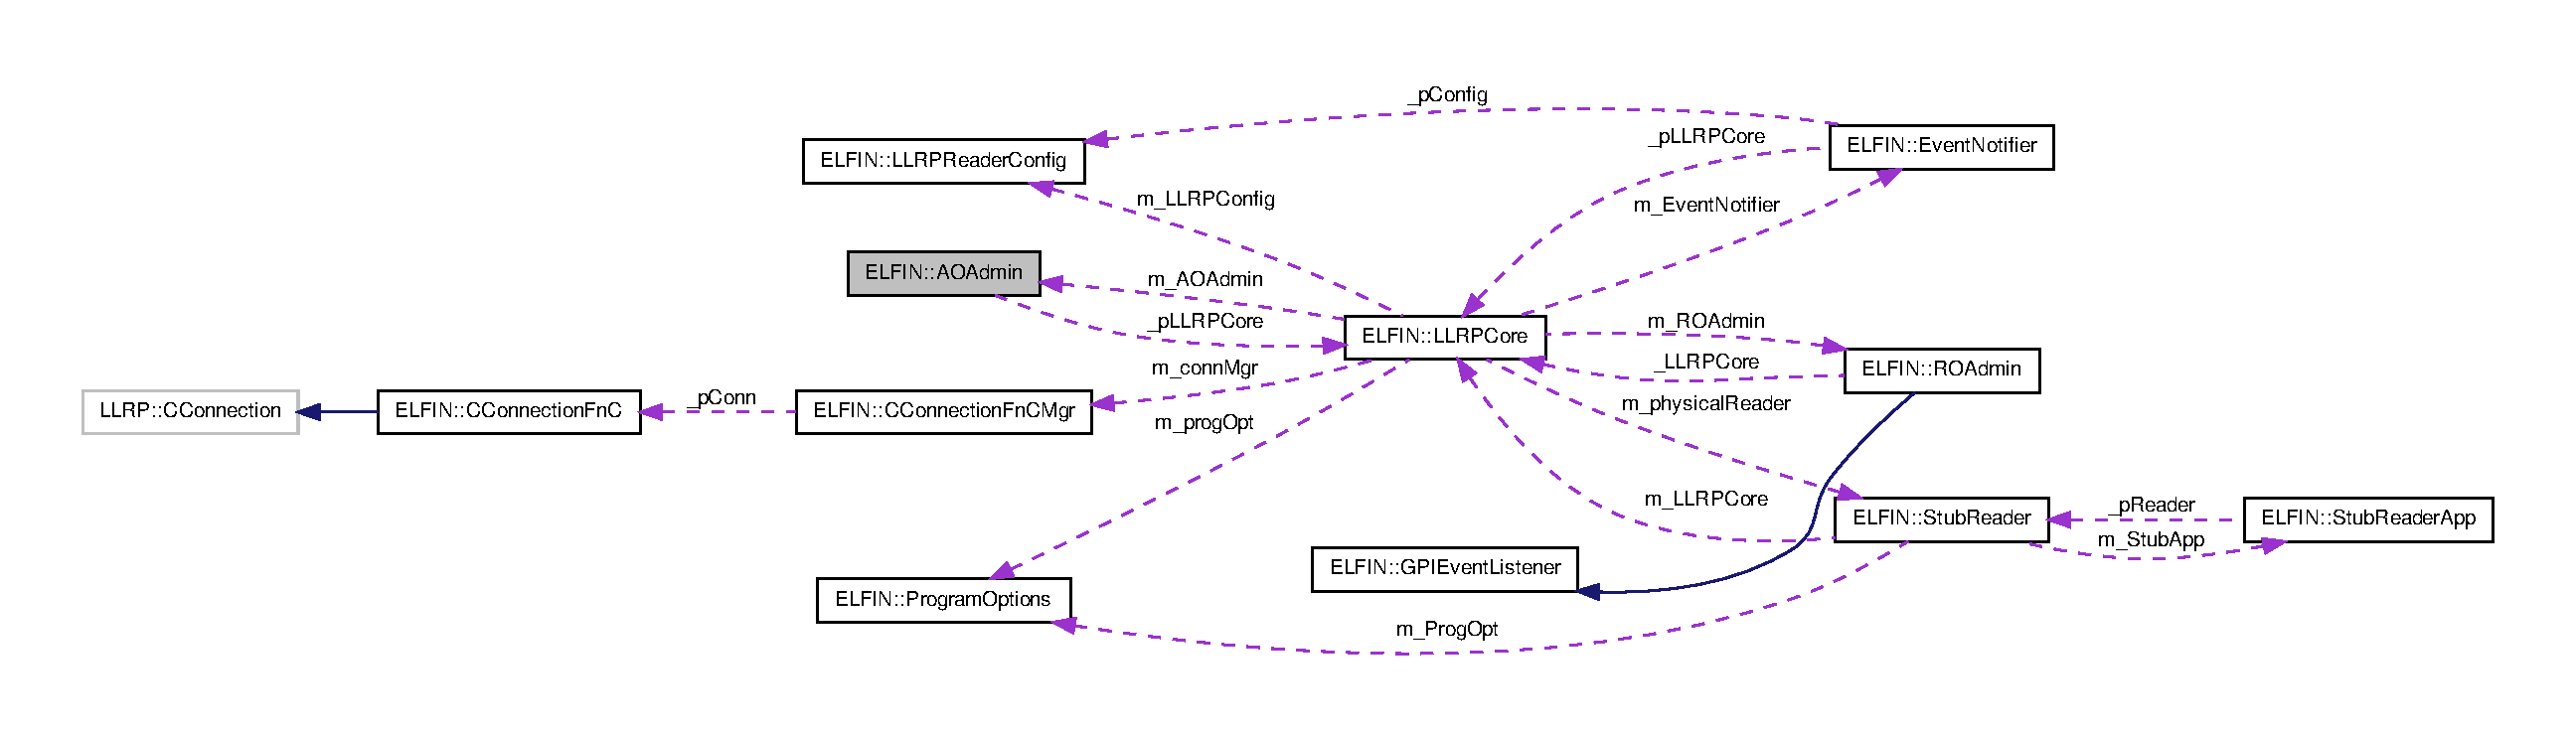
\includegraphics[width=350pt]{class_e_l_f_i_n_1_1_a_o_admin__coll__graph}
\end{center}
\end{figure}
\subsection*{Public Member Functions}
\begin{DoxyCompactItemize}
\item 
\hyperlink{class_e_l_f_i_n_1_1_a_o_admin_a2e1b2f780de7a4d3312eb0c4d5a9e9cc}{A\-O\-Admin} (\hyperlink{class_e_l_f_i_n_1_1_l_l_r_p_core}{L\-L\-R\-P\-Core} $\ast$\-\_\-\-\_\-p\-L\-L\-R\-P\-Core)
\begin{DoxyCompactList}\small\item\em Constructor of \hyperlink{class_e_l_f_i_n_1_1_a_o_admin}{A\-O\-Admin} class. \end{DoxyCompactList}\item 
\hyperlink{class_e_l_f_i_n_1_1_a_o_admin_a06a9286b19631ab519000d86ed81c29b}{$\sim$\-A\-O\-Admin} ()
\begin{DoxyCompactList}\small\item\em Destructor of \hyperlink{class_e_l_f_i_n_1_1_a_o_admin}{A\-O\-Admin} class. \end{DoxyCompactList}\item 
int \hyperlink{class_e_l_f_i_n_1_1_a_o_admin_a8f0296aef7586d378be8a390f4167e3d}{enable\-Access\-Spec} (L\-L\-R\-P\-::llrp\-\_\-u32\-\_\-t a\-Access\-Spec\-I\-D)
\begin{DoxyCompactList}\small\item\em Enable the Access\-Spec. If the given Access\-Spec I\-D is 0, enable all Access\-Spec. \end{DoxyCompactList}\item 
int \hyperlink{class_e_l_f_i_n_1_1_a_o_admin_ac493ec01485f6a3359958919ddace01a}{add\-Access\-Spec} (L\-L\-R\-P\-::\-C\-Access\-Spec $\ast$a\-Access\-Spec)
\begin{DoxyCompactList}\small\item\em Add the given Access\-Spec. \end{DoxyCompactList}\item 
int \hyperlink{class_e_l_f_i_n_1_1_a_o_admin_ad93a4f9cb1c041471b0cb451fb06c5c1}{disable\-Access\-Spec} (L\-L\-R\-P\-::llrp\-\_\-u32\-\_\-t a\-Access\-Spec\-I\-D)
\begin{DoxyCompactList}\small\item\em Disable the Access\-Spec. If the given Access\-Spec I\-D is 0, disable all Access\-Spec. \end{DoxyCompactList}\item 
int \hyperlink{class_e_l_f_i_n_1_1_a_o_admin_a1b8efe946d80673b80416c7103018967}{delete\-Access\-Spec} (L\-L\-R\-P\-::llrp\-\_\-u32\-\_\-t a\-Access\-Spec\-I\-D)
\begin{DoxyCompactList}\small\item\em Delete the Access\-Spec. If the given Access\-Spec I\-D is 0, delete all Access\-Spec. \end{DoxyCompactList}\item 
std\-::vector$<$ L\-L\-R\-P\-::\-C\-Access\-Spec $\ast$ $>$ $\ast$ \hyperlink{class_e_l_f_i_n_1_1_a_o_admin_a5bfd2b0c57333304d53c5cea1cdff0f0}{get\-Access\-Specs} ()
\begin{DoxyCompactList}\small\item\em Store the pointer of all Access\-Specs to vector, and return it. \end{DoxyCompactList}\end{DoxyCompactItemize}
{\bf }\par
\begin{DoxyCompactItemize}
\item 
E\-L\-F\-I\-N\-::\-A\-O\-Map\-::iterator \hyperlink{class_e_l_f_i_n_1_1_a_o_admin_abd2953505ee15f57f80bf8d5c094297b}{begin\-A\-O\-Map} ()
\begin{DoxyCompactList}\small\item\em Iterator access method. \end{DoxyCompactList}\item 
E\-L\-F\-I\-N\-::\-A\-O\-Map\-::iterator \hyperlink{class_e_l_f_i_n_1_1_a_o_admin_aafe66a19da5c9033fcd73142981e96c5}{end\-A\-O\-Map} ()
\begin{DoxyCompactList}\small\item\em Iterator access method. \end{DoxyCompactList}\item 
int \hyperlink{class_e_l_f_i_n_1_1_a_o_admin_a09f489a82b270c4f3d26c2b93241a544}{count\-A\-O\-Map} ()
\begin{DoxyCompactList}\small\item\em Iterator access method. \end{DoxyCompactList}\end{DoxyCompactItemize}

\subsection*{Private Attributes}
\begin{DoxyCompactItemize}
\item 
\hypertarget{class_e_l_f_i_n_1_1_a_o_admin_ab9467e08db0f0365ada52fcbfba76abb}{\hyperlink{class_e_l_f_i_n_1_1_l_l_r_p_core}{E\-L\-F\-I\-N\-::\-L\-L\-R\-P\-Core} $\ast$ {\bfseries \-\_\-p\-L\-L\-R\-P\-Core}}\label{class_e_l_f_i_n_1_1_a_o_admin_ab9467e08db0f0365ada52fcbfba76abb}

\item 
C\-A\-O\-Map \hyperlink{class_e_l_f_i_n_1_1_a_o_admin_acd6bbfe5fce9e349e5b563b73750e191}{\-\_\-\-C\-A\-O\-Map}
\begin{DoxyCompactList}\small\item\em C\-Access\-Spec container. \end{DoxyCompactList}\item 
A\-O\-Map \hyperlink{class_e_l_f_i_n_1_1_a_o_admin_aee21fd9858d0f8e3c897e47faaa53483}{\-\_\-\-A\-O\-Map}
\begin{DoxyCompactList}\small\item\em Access Operation container. \end{DoxyCompactList}\end{DoxyCompactItemize}


\subsection{Detailed Description}
A\-O\-Admin(\-Access Operation Admin) class manages states of Access\-Specs. 

Definition at line 23 of file A\-O\-Admin.\-h.



\subsection{Constructor \& Destructor Documentation}
\hypertarget{class_e_l_f_i_n_1_1_a_o_admin_a2e1b2f780de7a4d3312eb0c4d5a9e9cc}{\index{E\-L\-F\-I\-N\-::\-A\-O\-Admin@{E\-L\-F\-I\-N\-::\-A\-O\-Admin}!A\-O\-Admin@{A\-O\-Admin}}
\index{A\-O\-Admin@{A\-O\-Admin}!ELFIN::AOAdmin@{E\-L\-F\-I\-N\-::\-A\-O\-Admin}}
\subsubsection[{A\-O\-Admin}]{\setlength{\rightskip}{0pt plus 5cm}E\-L\-F\-I\-N\-::\-A\-O\-Admin\-::\-A\-O\-Admin (
\begin{DoxyParamCaption}
\item[{{\bf L\-L\-R\-P\-Core} $\ast$}]{\-\_\-\-\_\-p\-L\-L\-R\-P\-Core}
\end{DoxyParamCaption}
)}}\label{class_e_l_f_i_n_1_1_a_o_admin_a2e1b2f780de7a4d3312eb0c4d5a9e9cc}


Constructor of \hyperlink{class_e_l_f_i_n_1_1_a_o_admin}{A\-O\-Admin} class. 



Definition at line 190 of file A\-O\-Admin.\-cpp.

\hypertarget{class_e_l_f_i_n_1_1_a_o_admin_a06a9286b19631ab519000d86ed81c29b}{\index{E\-L\-F\-I\-N\-::\-A\-O\-Admin@{E\-L\-F\-I\-N\-::\-A\-O\-Admin}!$\sim$\-A\-O\-Admin@{$\sim$\-A\-O\-Admin}}
\index{$\sim$\-A\-O\-Admin@{$\sim$\-A\-O\-Admin}!ELFIN::AOAdmin@{E\-L\-F\-I\-N\-::\-A\-O\-Admin}}
\subsubsection[{$\sim$\-A\-O\-Admin}]{\setlength{\rightskip}{0pt plus 5cm}E\-L\-F\-I\-N\-::\-A\-O\-Admin\-::$\sim$\-A\-O\-Admin (
\begin{DoxyParamCaption}
{}
\end{DoxyParamCaption}
)}}\label{class_e_l_f_i_n_1_1_a_o_admin_a06a9286b19631ab519000d86ed81c29b}


Destructor of \hyperlink{class_e_l_f_i_n_1_1_a_o_admin}{A\-O\-Admin} class. 



Definition at line 194 of file A\-O\-Admin.\-cpp.



\subsection{Member Function Documentation}
\hypertarget{class_e_l_f_i_n_1_1_a_o_admin_ac493ec01485f6a3359958919ddace01a}{\index{E\-L\-F\-I\-N\-::\-A\-O\-Admin@{E\-L\-F\-I\-N\-::\-A\-O\-Admin}!add\-Access\-Spec@{add\-Access\-Spec}}
\index{add\-Access\-Spec@{add\-Access\-Spec}!ELFIN::AOAdmin@{E\-L\-F\-I\-N\-::\-A\-O\-Admin}}
\subsubsection[{add\-Access\-Spec}]{\setlength{\rightskip}{0pt plus 5cm}int E\-L\-F\-I\-N\-::\-A\-O\-Admin\-::add\-Access\-Spec (
\begin{DoxyParamCaption}
\item[{L\-L\-R\-P\-::\-C\-Access\-Spec $\ast$}]{a\-Access\-Spec}
\end{DoxyParamCaption}
)}}\label{class_e_l_f_i_n_1_1_a_o_admin_ac493ec01485f6a3359958919ddace01a}


Add the given Access\-Spec. 

\begin{DoxyRefDesc}{Todo}
\item[\hyperlink{todo__todo000009}{Todo}]In case there are multiple Access\-Specs that get matched during a Tag\-Spec lookup, the Reader S\-H\-A\-L\-L only execute the first enabled Access\-Spec that matches, where the ordering of the Access\-Specs is the order in which the Access\-Specs were created by the Client. (L\-L\-R\-P Spec 12.\-2.\-1.\-2) \end{DoxyRefDesc}


Definition at line 65 of file A\-O\-Admin.\-cpp.

\hypertarget{class_e_l_f_i_n_1_1_a_o_admin_abd2953505ee15f57f80bf8d5c094297b}{\index{E\-L\-F\-I\-N\-::\-A\-O\-Admin@{E\-L\-F\-I\-N\-::\-A\-O\-Admin}!begin\-A\-O\-Map@{begin\-A\-O\-Map}}
\index{begin\-A\-O\-Map@{begin\-A\-O\-Map}!ELFIN::AOAdmin@{E\-L\-F\-I\-N\-::\-A\-O\-Admin}}
\subsubsection[{begin\-A\-O\-Map}]{\setlength{\rightskip}{0pt plus 5cm}E\-L\-F\-I\-N\-::\-A\-O\-Map\-::iterator E\-L\-F\-I\-N\-::\-A\-O\-Admin\-::begin\-A\-O\-Map (
\begin{DoxyParamCaption}
{}
\end{DoxyParamCaption}
)}}\label{class_e_l_f_i_n_1_1_a_o_admin_abd2953505ee15f57f80bf8d5c094297b}


Iterator access method. 



Definition at line 178 of file A\-O\-Admin.\-cpp.

\hypertarget{class_e_l_f_i_n_1_1_a_o_admin_a09f489a82b270c4f3d26c2b93241a544}{\index{E\-L\-F\-I\-N\-::\-A\-O\-Admin@{E\-L\-F\-I\-N\-::\-A\-O\-Admin}!count\-A\-O\-Map@{count\-A\-O\-Map}}
\index{count\-A\-O\-Map@{count\-A\-O\-Map}!ELFIN::AOAdmin@{E\-L\-F\-I\-N\-::\-A\-O\-Admin}}
\subsubsection[{count\-A\-O\-Map}]{\setlength{\rightskip}{0pt plus 5cm}int E\-L\-F\-I\-N\-::\-A\-O\-Admin\-::count\-A\-O\-Map (
\begin{DoxyParamCaption}
{}
\end{DoxyParamCaption}
)}}\label{class_e_l_f_i_n_1_1_a_o_admin_a09f489a82b270c4f3d26c2b93241a544}


Iterator access method. 



Definition at line 186 of file A\-O\-Admin.\-cpp.

\hypertarget{class_e_l_f_i_n_1_1_a_o_admin_a1b8efe946d80673b80416c7103018967}{\index{E\-L\-F\-I\-N\-::\-A\-O\-Admin@{E\-L\-F\-I\-N\-::\-A\-O\-Admin}!delete\-Access\-Spec@{delete\-Access\-Spec}}
\index{delete\-Access\-Spec@{delete\-Access\-Spec}!ELFIN::AOAdmin@{E\-L\-F\-I\-N\-::\-A\-O\-Admin}}
\subsubsection[{delete\-Access\-Spec}]{\setlength{\rightskip}{0pt plus 5cm}int E\-L\-F\-I\-N\-::\-A\-O\-Admin\-::delete\-Access\-Spec (
\begin{DoxyParamCaption}
\item[{L\-L\-R\-P\-::llrp\-\_\-u32\-\_\-t}]{a\-Access\-Spec\-I\-D}
\end{DoxyParamCaption}
)}}\label{class_e_l_f_i_n_1_1_a_o_admin_a1b8efe946d80673b80416c7103018967}


Delete the Access\-Spec. If the given Access\-Spec I\-D is 0, delete all Access\-Spec. 



Definition at line 124 of file A\-O\-Admin.\-cpp.

\hypertarget{class_e_l_f_i_n_1_1_a_o_admin_ad93a4f9cb1c041471b0cb451fb06c5c1}{\index{E\-L\-F\-I\-N\-::\-A\-O\-Admin@{E\-L\-F\-I\-N\-::\-A\-O\-Admin}!disable\-Access\-Spec@{disable\-Access\-Spec}}
\index{disable\-Access\-Spec@{disable\-Access\-Spec}!ELFIN::AOAdmin@{E\-L\-F\-I\-N\-::\-A\-O\-Admin}}
\subsubsection[{disable\-Access\-Spec}]{\setlength{\rightskip}{0pt plus 5cm}int E\-L\-F\-I\-N\-::\-A\-O\-Admin\-::disable\-Access\-Spec (
\begin{DoxyParamCaption}
\item[{L\-L\-R\-P\-::llrp\-\_\-u32\-\_\-t}]{a\-Access\-Spec\-I\-D}
\end{DoxyParamCaption}
)}}\label{class_e_l_f_i_n_1_1_a_o_admin_ad93a4f9cb1c041471b0cb451fb06c5c1}


Disable the Access\-Spec. If the given Access\-Spec I\-D is 0, disable all Access\-Spec. 



Definition at line 83 of file A\-O\-Admin.\-cpp.

\hypertarget{class_e_l_f_i_n_1_1_a_o_admin_a8f0296aef7586d378be8a390f4167e3d}{\index{E\-L\-F\-I\-N\-::\-A\-O\-Admin@{E\-L\-F\-I\-N\-::\-A\-O\-Admin}!enable\-Access\-Spec@{enable\-Access\-Spec}}
\index{enable\-Access\-Spec@{enable\-Access\-Spec}!ELFIN::AOAdmin@{E\-L\-F\-I\-N\-::\-A\-O\-Admin}}
\subsubsection[{enable\-Access\-Spec}]{\setlength{\rightskip}{0pt plus 5cm}int E\-L\-F\-I\-N\-::\-A\-O\-Admin\-::enable\-Access\-Spec (
\begin{DoxyParamCaption}
\item[{L\-L\-R\-P\-::llrp\-\_\-u32\-\_\-t}]{a\-Access\-Spec\-I\-D}
\end{DoxyParamCaption}
)}}\label{class_e_l_f_i_n_1_1_a_o_admin_a8f0296aef7586d378be8a390f4167e3d}


Enable the Access\-Spec. If the given Access\-Spec I\-D is 0, enable all Access\-Spec. 



Definition at line 15 of file A\-O\-Admin.\-cpp.

\hypertarget{class_e_l_f_i_n_1_1_a_o_admin_aafe66a19da5c9033fcd73142981e96c5}{\index{E\-L\-F\-I\-N\-::\-A\-O\-Admin@{E\-L\-F\-I\-N\-::\-A\-O\-Admin}!end\-A\-O\-Map@{end\-A\-O\-Map}}
\index{end\-A\-O\-Map@{end\-A\-O\-Map}!ELFIN::AOAdmin@{E\-L\-F\-I\-N\-::\-A\-O\-Admin}}
\subsubsection[{end\-A\-O\-Map}]{\setlength{\rightskip}{0pt plus 5cm}E\-L\-F\-I\-N\-::\-A\-O\-Map\-::iterator E\-L\-F\-I\-N\-::\-A\-O\-Admin\-::end\-A\-O\-Map (
\begin{DoxyParamCaption}
{}
\end{DoxyParamCaption}
)}}\label{class_e_l_f_i_n_1_1_a_o_admin_aafe66a19da5c9033fcd73142981e96c5}


Iterator access method. 



Definition at line 182 of file A\-O\-Admin.\-cpp.

\hypertarget{class_e_l_f_i_n_1_1_a_o_admin_a5bfd2b0c57333304d53c5cea1cdff0f0}{\index{E\-L\-F\-I\-N\-::\-A\-O\-Admin@{E\-L\-F\-I\-N\-::\-A\-O\-Admin}!get\-Access\-Specs@{get\-Access\-Specs}}
\index{get\-Access\-Specs@{get\-Access\-Specs}!ELFIN::AOAdmin@{E\-L\-F\-I\-N\-::\-A\-O\-Admin}}
\subsubsection[{get\-Access\-Specs}]{\setlength{\rightskip}{0pt plus 5cm}std\-::vector$<$ L\-L\-R\-P\-::\-C\-Access\-Spec $\ast$ $>$ $\ast$ E\-L\-F\-I\-N\-::\-A\-O\-Admin\-::get\-Access\-Specs (
\begin{DoxyParamCaption}
{}
\end{DoxyParamCaption}
)}}\label{class_e_l_f_i_n_1_1_a_o_admin_a5bfd2b0c57333304d53c5cea1cdff0f0}


Store the pointer of all Access\-Specs to vector, and return it. 

\begin{DoxyWarning}{Warning}
You should delete the returned vector to avoid memory leakage.\par
And you must not delete the Access\-Specs in the vector, because they are original ones. 
\end{DoxyWarning}


Definition at line 170 of file A\-O\-Admin.\-cpp.



\subsection{Member Data Documentation}
\hypertarget{class_e_l_f_i_n_1_1_a_o_admin_aee21fd9858d0f8e3c897e47faaa53483}{\index{E\-L\-F\-I\-N\-::\-A\-O\-Admin@{E\-L\-F\-I\-N\-::\-A\-O\-Admin}!\-\_\-\-A\-O\-Map@{\-\_\-\-A\-O\-Map}}
\index{\-\_\-\-A\-O\-Map@{\-\_\-\-A\-O\-Map}!ELFIN::AOAdmin@{E\-L\-F\-I\-N\-::\-A\-O\-Admin}}
\subsubsection[{\-\_\-\-A\-O\-Map}]{\setlength{\rightskip}{0pt plus 5cm}A\-O\-Map E\-L\-F\-I\-N\-::\-A\-O\-Admin\-::\-\_\-\-A\-O\-Map\hspace{0.3cm}{\ttfamily [private]}}}\label{class_e_l_f_i_n_1_1_a_o_admin_aee21fd9858d0f8e3c897e47faaa53483}


Access Operation container. 



Definition at line 52 of file A\-O\-Admin.\-h.

\hypertarget{class_e_l_f_i_n_1_1_a_o_admin_acd6bbfe5fce9e349e5b563b73750e191}{\index{E\-L\-F\-I\-N\-::\-A\-O\-Admin@{E\-L\-F\-I\-N\-::\-A\-O\-Admin}!\-\_\-\-C\-A\-O\-Map@{\-\_\-\-C\-A\-O\-Map}}
\index{\-\_\-\-C\-A\-O\-Map@{\-\_\-\-C\-A\-O\-Map}!ELFIN::AOAdmin@{E\-L\-F\-I\-N\-::\-A\-O\-Admin}}
\subsubsection[{\-\_\-\-C\-A\-O\-Map}]{\setlength{\rightskip}{0pt plus 5cm}C\-A\-O\-Map E\-L\-F\-I\-N\-::\-A\-O\-Admin\-::\-\_\-\-C\-A\-O\-Map\hspace{0.3cm}{\ttfamily [private]}}}\label{class_e_l_f_i_n_1_1_a_o_admin_acd6bbfe5fce9e349e5b563b73750e191}


C\-Access\-Spec container. 



Definition at line 50 of file A\-O\-Admin.\-h.



The documentation for this class was generated from the following files\-:\begin{DoxyCompactItemize}
\item 
elfin\-\_\-src/\hyperlink{_a_o_admin_8h}{A\-O\-Admin.\-h}\item 
elfin\-\_\-src/\hyperlink{_a_o_admin_8cpp}{A\-O\-Admin.\-cpp}\end{DoxyCompactItemize}

\hypertarget{class_e_l_f_i_n_1_1_c_connection_fn_c}{\section{E\-L\-F\-I\-N\-:\-:C\-Connection\-Fn\-C Class Reference}
\label{class_e_l_f_i_n_1_1_c_connection_fn_c}\index{E\-L\-F\-I\-N\-::\-C\-Connection\-Fn\-C@{E\-L\-F\-I\-N\-::\-C\-Connection\-Fn\-C}}
}


Inherits L\-L\-R\-P\-::\-C\-Connection class. It has additional methods for Reader role.  




{\ttfamily \#include $<$C\-Connection\-Fn\-C.\-h$>$}



Inheritance diagram for E\-L\-F\-I\-N\-:\-:C\-Connection\-Fn\-C\-:
\nopagebreak
\begin{figure}[H]
\begin{center}
\leavevmode
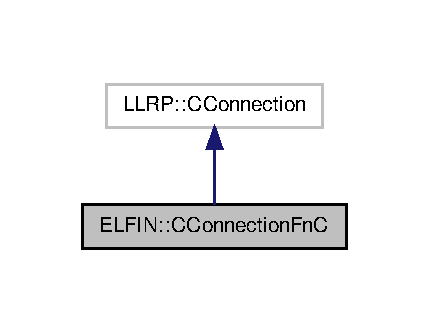
\includegraphics[width=206pt]{class_e_l_f_i_n_1_1_c_connection_fn_c__inherit__graph}
\end{center}
\end{figure}


Collaboration diagram for E\-L\-F\-I\-N\-:\-:C\-Connection\-Fn\-C\-:
\nopagebreak
\begin{figure}[H]
\begin{center}
\leavevmode
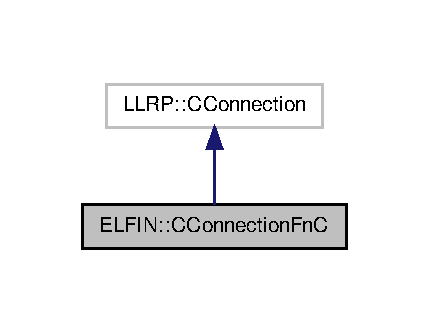
\includegraphics[width=206pt]{class_e_l_f_i_n_1_1_c_connection_fn_c__coll__graph}
\end{center}
\end{figure}
\subsection*{Public Member Functions}
\begin{DoxyCompactItemize}
\item 
\hyperlink{class_e_l_f_i_n_1_1_c_connection_fn_c_a7f75c79f20a7d439266094d826dfca23}{C\-Connection\-Fn\-C} (const L\-L\-R\-P\-::\-C\-Type\-Registry $\ast$p\-Type\-Registry, unsigned int n\-Buffer\-Size, unsigned int port\-Num)
\begin{DoxyCompactList}\small\item\em Constructor of \hyperlink{class_e_l_f_i_n_1_1_c_connection_fn_c}{C\-Connection\-Fn\-C} class. \end{DoxyCompactList}\item 
\hyperlink{class_e_l_f_i_n_1_1_c_connection_fn_c_a0f88955ac24427bc224c8970a3e40016}{$\sim$\-C\-Connection\-Fn\-C} (void)
\begin{DoxyCompactList}\small\item\em Destructor of \hyperlink{class_e_l_f_i_n_1_1_c_connection_fn_c}{C\-Connection\-Fn\-C} class. \end{DoxyCompactList}\item 
int \hyperlink{class_e_l_f_i_n_1_1_c_connection_fn_c_a36cce7a57378de89fc5a03fb39092348}{close\-Connection\-To\-Fn\-C} (int \-\_\-\-\_\-is\-Reader\-Initiated)
\begin{DoxyCompactList}\small\item\em Close connection to the Fn\-C server. \end{DoxyCompactList}\item 
int \hyperlink{class_e_l_f_i_n_1_1_c_connection_fn_c_aade173f8606de8d853344752b4e18678}{open\-Connection\-To\-Fn\-C} (const char $\ast$p\-Reader\-Host\-Name)
\begin{DoxyCompactList}\small\item\em Initiate connection to the Fn\-C server (client mode) \end{DoxyCompactList}\item 
int \hyperlink{class_e_l_f_i_n_1_1_c_connection_fn_c_a452088817621707bb340b6b4b67dc995}{accept\-Connection\-From\-Client} ()
\begin{DoxyCompactList}\small\item\em Wait for connection from the Fn\-C server (server mode) \end{DoxyCompactList}\end{DoxyCompactItemize}


\subsection{Detailed Description}
Inherits L\-L\-R\-P\-::\-C\-Connection class. It has additional methods for Reader role. 

\begin{DoxyRemark}{Remarks}
Additional methods are moved to C\-Connection of L\-T\-K. Now, this class just acts similar to the proxy of L\-L\-R\-P\-::\-C\-Connection class. 
\end{DoxyRemark}


Definition at line 28 of file C\-Connection\-Fn\-C.\-h.



\subsection{Constructor \& Destructor Documentation}
\hypertarget{class_e_l_f_i_n_1_1_c_connection_fn_c_a7f75c79f20a7d439266094d826dfca23}{\index{E\-L\-F\-I\-N\-::\-C\-Connection\-Fn\-C@{E\-L\-F\-I\-N\-::\-C\-Connection\-Fn\-C}!C\-Connection\-Fn\-C@{C\-Connection\-Fn\-C}}
\index{C\-Connection\-Fn\-C@{C\-Connection\-Fn\-C}!ELFIN::CConnectionFnC@{E\-L\-F\-I\-N\-::\-C\-Connection\-Fn\-C}}
\subsubsection[{C\-Connection\-Fn\-C}]{\setlength{\rightskip}{0pt plus 5cm}E\-L\-F\-I\-N\-::\-C\-Connection\-Fn\-C\-::\-C\-Connection\-Fn\-C (
\begin{DoxyParamCaption}
\item[{const L\-L\-R\-P\-::\-C\-Type\-Registry $\ast$}]{p\-Type\-Registry, }
\item[{unsigned int}]{n\-Buffer\-Size, }
\item[{unsigned int}]{port\-Num}
\end{DoxyParamCaption}
)}}\label{class_e_l_f_i_n_1_1_c_connection_fn_c_a7f75c79f20a7d439266094d826dfca23}


Constructor of \hyperlink{class_e_l_f_i_n_1_1_c_connection_fn_c}{C\-Connection\-Fn\-C} class. 



Definition at line 55 of file C\-Connection\-Fn\-C.\-cpp.

\hypertarget{class_e_l_f_i_n_1_1_c_connection_fn_c_a0f88955ac24427bc224c8970a3e40016}{\index{E\-L\-F\-I\-N\-::\-C\-Connection\-Fn\-C@{E\-L\-F\-I\-N\-::\-C\-Connection\-Fn\-C}!$\sim$\-C\-Connection\-Fn\-C@{$\sim$\-C\-Connection\-Fn\-C}}
\index{$\sim$\-C\-Connection\-Fn\-C@{$\sim$\-C\-Connection\-Fn\-C}!ELFIN::CConnectionFnC@{E\-L\-F\-I\-N\-::\-C\-Connection\-Fn\-C}}
\subsubsection[{$\sim$\-C\-Connection\-Fn\-C}]{\setlength{\rightskip}{0pt plus 5cm}E\-L\-F\-I\-N\-::\-C\-Connection\-Fn\-C\-::$\sim$\-C\-Connection\-Fn\-C (
\begin{DoxyParamCaption}
\item[{void}]{}
\end{DoxyParamCaption}
)}}\label{class_e_l_f_i_n_1_1_c_connection_fn_c_a0f88955ac24427bc224c8970a3e40016}


Destructor of \hyperlink{class_e_l_f_i_n_1_1_c_connection_fn_c}{C\-Connection\-Fn\-C} class. 



Definition at line 61 of file C\-Connection\-Fn\-C.\-cpp.



\subsection{Member Function Documentation}
\hypertarget{class_e_l_f_i_n_1_1_c_connection_fn_c_a452088817621707bb340b6b4b67dc995}{\index{E\-L\-F\-I\-N\-::\-C\-Connection\-Fn\-C@{E\-L\-F\-I\-N\-::\-C\-Connection\-Fn\-C}!accept\-Connection\-From\-Client@{accept\-Connection\-From\-Client}}
\index{accept\-Connection\-From\-Client@{accept\-Connection\-From\-Client}!ELFIN::CConnectionFnC@{E\-L\-F\-I\-N\-::\-C\-Connection\-Fn\-C}}
\subsubsection[{accept\-Connection\-From\-Client}]{\setlength{\rightskip}{0pt plus 5cm}int E\-L\-F\-I\-N\-::\-C\-Connection\-Fn\-C\-::accept\-Connection\-From\-Client (
\begin{DoxyParamCaption}
{}
\end{DoxyParamCaption}
)}}\label{class_e_l_f_i_n_1_1_c_connection_fn_c_a452088817621707bb340b6b4b67dc995}


Wait for connection from the Fn\-C server (server mode) 



Definition at line 81 of file C\-Connection\-Fn\-C.\-cpp.

\hypertarget{class_e_l_f_i_n_1_1_c_connection_fn_c_a36cce7a57378de89fc5a03fb39092348}{\index{E\-L\-F\-I\-N\-::\-C\-Connection\-Fn\-C@{E\-L\-F\-I\-N\-::\-C\-Connection\-Fn\-C}!close\-Connection\-To\-Fn\-C@{close\-Connection\-To\-Fn\-C}}
\index{close\-Connection\-To\-Fn\-C@{close\-Connection\-To\-Fn\-C}!ELFIN::CConnectionFnC@{E\-L\-F\-I\-N\-::\-C\-Connection\-Fn\-C}}
\subsubsection[{close\-Connection\-To\-Fn\-C}]{\setlength{\rightskip}{0pt plus 5cm}int E\-L\-F\-I\-N\-::\-C\-Connection\-Fn\-C\-::close\-Connection\-To\-Fn\-C (
\begin{DoxyParamCaption}
\item[{int}]{\-\_\-\-\_\-is\-Reader\-Initiated}
\end{DoxyParamCaption}
)}}\label{class_e_l_f_i_n_1_1_c_connection_fn_c_a36cce7a57378de89fc5a03fb39092348}


Close connection to the Fn\-C server. 

\begin{DoxyRemark}{Remarks}
If \-\_\-\-\_\-is\-Reader\-Initiated = 0, then close listening socket and communication socket.\par
If not, just close communication socket.\par
The method that closes communication socket is close\-Connection\-To\-Reader(adopted from L\-T\-K), but what it does is just closing the socket. 
\end{DoxyRemark}


Definition at line 70 of file C\-Connection\-Fn\-C.\-cpp.

\hypertarget{class_e_l_f_i_n_1_1_c_connection_fn_c_aade173f8606de8d853344752b4e18678}{\index{E\-L\-F\-I\-N\-::\-C\-Connection\-Fn\-C@{E\-L\-F\-I\-N\-::\-C\-Connection\-Fn\-C}!open\-Connection\-To\-Fn\-C@{open\-Connection\-To\-Fn\-C}}
\index{open\-Connection\-To\-Fn\-C@{open\-Connection\-To\-Fn\-C}!ELFIN::CConnectionFnC@{E\-L\-F\-I\-N\-::\-C\-Connection\-Fn\-C}}
\subsubsection[{open\-Connection\-To\-Fn\-C}]{\setlength{\rightskip}{0pt plus 5cm}int E\-L\-F\-I\-N\-::\-C\-Connection\-Fn\-C\-::open\-Connection\-To\-Fn\-C (
\begin{DoxyParamCaption}
\item[{const char $\ast$}]{p\-Reader\-Host\-Name}
\end{DoxyParamCaption}
)}}\label{class_e_l_f_i_n_1_1_c_connection_fn_c_aade173f8606de8d853344752b4e18678}


Initiate connection to the Fn\-C server (client mode) 



Definition at line 76 of file C\-Connection\-Fn\-C.\-cpp.



The documentation for this class was generated from the following files\-:\begin{DoxyCompactItemize}
\item 
elfin\-\_\-src/\hyperlink{_c_connection_fn_c_8h}{C\-Connection\-Fn\-C.\-h}\item 
elfin\-\_\-src/\hyperlink{_c_connection_fn_c_8cpp}{C\-Connection\-Fn\-C.\-cpp}\end{DoxyCompactItemize}

\hypertarget{class_e_l_f_i_n_1_1_c_connection_fn_c_mgr}{\section{E\-L\-F\-I\-N\-:\-:C\-Connection\-Fn\-C\-Mgr Class Reference}
\label{class_e_l_f_i_n_1_1_c_connection_fn_c_mgr}\index{E\-L\-F\-I\-N\-::\-C\-Connection\-Fn\-C\-Mgr@{E\-L\-F\-I\-N\-::\-C\-Connection\-Fn\-C\-Mgr}}
}


Inherits C\-Connection class. It has additional methods for Reader role.  




{\ttfamily \#include $<$C\-Connection\-Fn\-C\-Mgr.\-h$>$}



Collaboration diagram for E\-L\-F\-I\-N\-:\-:C\-Connection\-Fn\-C\-Mgr\-:
\nopagebreak
\begin{figure}[H]
\begin{center}
\leavevmode
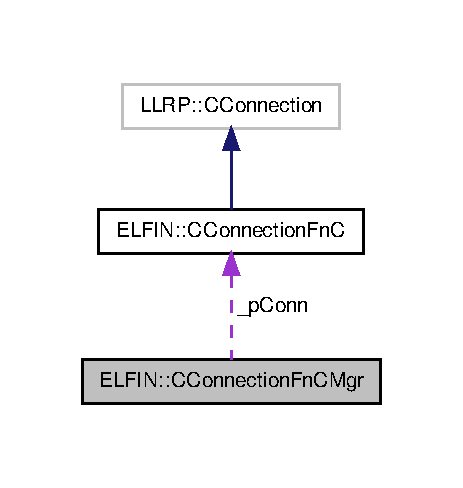
\includegraphics[width=222pt]{class_e_l_f_i_n_1_1_c_connection_fn_c_mgr__coll__graph}
\end{center}
\end{figure}
\subsection*{Public Member Functions}
\begin{DoxyCompactItemize}
\item 
\hyperlink{class_e_l_f_i_n_1_1_c_connection_fn_c_mgr_a59be0f0430708f38db8876fad91ed523}{C\-Connection\-Fn\-C\-Mgr} ()
\begin{DoxyCompactList}\small\item\em Constructor of \hyperlink{class_e_l_f_i_n_1_1_c_connection_fn_c_mgr}{C\-Connection\-Fn\-C\-Mgr} class. \end{DoxyCompactList}\item 
\hyperlink{class_e_l_f_i_n_1_1_c_connection_fn_c_mgr_a1237e5c2eac852fd12bc3547b11bcd99}{$\sim$\-C\-Connection\-Fn\-C\-Mgr} (void)
\begin{DoxyCompactList}\small\item\em Destructor of C\-Connection\-Fnc\-Mgr class. \end{DoxyCompactList}\item 
int \hyperlink{class_e_l_f_i_n_1_1_c_connection_fn_c_mgr_ad1f332c28661f74ea58f7dfa4131fdad}{close\-Connection\-To\-Fn\-C} (int \-\_\-\-\_\-is\-Reader\-Initiated)
\begin{DoxyCompactList}\small\item\em Close connection to the Fn\-C server. \end{DoxyCompactList}\item 
int \hyperlink{class_e_l_f_i_n_1_1_c_connection_fn_c_mgr_af7ee83a8a9546bae5c1f83c4f282d56a}{send\-Connection\-Attempt\-Event} ()
\begin{DoxyCompactList}\small\item\em Send Connection\-Attempt\-Event notification to the Fn\-C server. \end{DoxyCompactList}\item 
int \hyperlink{class_e_l_f_i_n_1_1_c_connection_fn_c_mgr_a0b5e1d5ffe5b49aef3b52254d443ffef}{send\-Connection\-Close\-Event} ()
\begin{DoxyCompactList}\small\item\em Send Connection\-Close\-Event notification to the Fn\-C server. \end{DoxyCompactList}\item 
int \hyperlink{class_e_l_f_i_n_1_1_c_connection_fn_c_mgr_a0c54ce49b3d0c1219f30b89a77062493}{start\-Keepalive\-Thread} (int period\-M\-S)
\begin{DoxyCompactList}\small\item\em Create the keepalive thread. \end{DoxyCompactList}\item 
int \hyperlink{class_e_l_f_i_n_1_1_c_connection_fn_c_mgr_aa23c373881a560ef974cd1152ea76c43}{stop\-Keepalive\-Thread} ()
\begin{DoxyCompactList}\small\item\em Interrupt and stop the keepalive thread. \end{DoxyCompactList}\item 
void \hyperlink{class_e_l_f_i_n_1_1_c_connection_fn_c_mgr_a0f4f281ce4e577eb32c8df5052106fa3}{keepalive\-\_\-run} (int period\-M\-S)
\begin{DoxyCompactList}\small\item\em This method is used to make thread for keepalive. Send K\-E\-E\-P\-A\-L\-I\-V\-E message and check the K\-E\-E\-P\-A\-L\-I\-V\-E\-\_\-\-A\-C\-K periodically. \end{DoxyCompactList}\item 
int \hyperlink{class_e_l_f_i_n_1_1_c_connection_fn_c_mgr_afeb7e321253ac8ab298958393ecfabc5}{start\-Connection} (\hyperlink{class_e_l_f_i_n_1_1_program_options}{Program\-Options} $\ast$\-\_\-\-\_\-prog\-Opt)
\begin{DoxyCompactList}\small\item\em Start connection to the Fn\-C server. Checks reader\-\_\-initiated option to decide whether to initiate connection or wait for connection. \end{DoxyCompactList}\item 
L\-L\-R\-P\-::\-C\-Message $\ast$ \hyperlink{class_e_l_f_i_n_1_1_c_connection_fn_c_mgr_a615454a57231aca62fc6f0fa73df64dd}{recv\-Message} (int n\-Max\-M\-S)
\begin{DoxyCompactList}\small\item\em Receive the message in recv buffer. \end{DoxyCompactList}\item 
int \hyperlink{class_e_l_f_i_n_1_1_c_connection_fn_c_mgr_a48b283f30ddd8c2b0c2ed55e844085f8}{send\-Message} (L\-L\-R\-P\-::\-C\-Message $\ast$p\-Message)
\begin{DoxyCompactList}\small\item\em Queue the message to send buffer. \end{DoxyCompactList}\item 
const char $\ast$ \hyperlink{class_e_l_f_i_n_1_1_c_connection_fn_c_mgr_aea8e109f15d3f1fb041407e84fdfa934}{get\-Connect\-Error} (void)
\begin{DoxyCompactList}\small\item\em Get currently stored error string. \end{DoxyCompactList}\item 
const L\-L\-R\-P\-::\-C\-Error\-Details $\ast$ \hyperlink{class_e_l_f_i_n_1_1_c_connection_fn_c_mgr_ab2e92f43c03191db481e2270d829186e}{get\-Recv\-Error} (void)
\begin{DoxyCompactList}\small\item\em Get currenlty stored C\-Error\-Details. \end{DoxyCompactList}\item 
int \hyperlink{class_e_l_f_i_n_1_1_c_connection_fn_c_mgr_a0058da7de14d9c84027a46e3bde38d7e}{get\-Received\-Keepalive\-Id} ()
\begin{DoxyCompactList}\small\item\em Returns recently received keepalive id. \end{DoxyCompactList}\item 
void \hyperlink{class_e_l_f_i_n_1_1_c_connection_fn_c_mgr_a248b1ad1d6138f5ade40892f3afb5a68}{set\-Received\-Keepalive\-Id} (int \-\_\-\-\_\-received\-Keepalive\-I\-D)
\begin{DoxyCompactList}\small\item\em Set the \-\_\-received\-Keepalive\-I\-D id with given id. \end{DoxyCompactList}\item 
int \hyperlink{class_e_l_f_i_n_1_1_c_connection_fn_c_mgr_aa27f8bb83349b52dffe670824cfa0e53}{is\-Connected} ()
\begin{DoxyCompactList}\small\item\em Check whether the L\-L\-R\-P Wapper is connected to Fn\-C server. \end{DoxyCompactList}\end{DoxyCompactItemize}
\subsection*{Public Attributes}
\begin{DoxyCompactItemize}
\item 
\hypertarget{class_e_l_f_i_n_1_1_c_connection_fn_c_mgr_a61fa802e7be0de0e84bb6a802abf1ab8}{boost\-::thread $\ast$ {\bfseries \-\_\-keepalive\-Thread}}\label{class_e_l_f_i_n_1_1_c_connection_fn_c_mgr_a61fa802e7be0de0e84bb6a802abf1ab8}

\end{DoxyCompactItemize}
\subsection*{Private Member Functions}
\begin{DoxyCompactItemize}
\item 
int \hyperlink{class_e_l_f_i_n_1_1_c_connection_fn_c_mgr_a59b5a84c9df6d5e706ada67fc32ad0b5}{open\-Connection\-To\-Fn\-C} (const char $\ast$p\-Reader\-Host\-Name)
\begin{DoxyCompactList}\small\item\em Initiate connection to the Fn\-C server (client mode) \end{DoxyCompactList}\item 
int \hyperlink{class_e_l_f_i_n_1_1_c_connection_fn_c_mgr_af86142cdff404912079d5b48883378ad}{wait\-For\-Connection} ()
\begin{DoxyCompactList}\small\item\em Wait for connection from the Fn\-C server (server mode) \end{DoxyCompactList}\end{DoxyCompactItemize}
\subsection*{Private Attributes}
\begin{DoxyCompactItemize}
\item 
\hypertarget{class_e_l_f_i_n_1_1_c_connection_fn_c_mgr_af3dc94baee99fcf490529f5f83877d3c}{boost\-::recursive\-\_\-mutex {\bfseries \-\_\-send\-Mtx}}\label{class_e_l_f_i_n_1_1_c_connection_fn_c_mgr_af3dc94baee99fcf490529f5f83877d3c}

\item 
\hypertarget{class_e_l_f_i_n_1_1_c_connection_fn_c_mgr_aa290b78891b2051cc929966c888c020b}{\hyperlink{class_e_l_f_i_n_1_1_c_connection_fn_c}{C\-Connection\-Fn\-C} $\ast$ {\bfseries \-\_\-p\-Conn}}\label{class_e_l_f_i_n_1_1_c_connection_fn_c_mgr_aa290b78891b2051cc929966c888c020b}

\item 
\hypertarget{class_e_l_f_i_n_1_1_c_connection_fn_c_mgr_a4bcad4503a1df5c5f3aa89633ea60acf}{int {\bfseries \-\_\-port\-Num}}\label{class_e_l_f_i_n_1_1_c_connection_fn_c_mgr_a4bcad4503a1df5c5f3aa89633ea60acf}

\item 
\hypertarget{class_e_l_f_i_n_1_1_c_connection_fn_c_mgr_a06f5ea6a6b927aacce077f5f87a85b20}{int {\bfseries \-\_\-received\-Keepalive\-I\-D}}\label{class_e_l_f_i_n_1_1_c_connection_fn_c_mgr_a06f5ea6a6b927aacce077f5f87a85b20}

\item 
\hypertarget{class_e_l_f_i_n_1_1_c_connection_fn_c_mgr_ac094be115074540e3d5973f44f23ef24}{boost\-::mutex {\bfseries \-\_\-ka\-Mtx}}\label{class_e_l_f_i_n_1_1_c_connection_fn_c_mgr_ac094be115074540e3d5973f44f23ef24}

\item 
\hypertarget{class_e_l_f_i_n_1_1_c_connection_fn_c_mgr_a56a8b82f5207f52aa01090de57db36f4}{int {\bfseries \-\_\-ka\-Stop}}\label{class_e_l_f_i_n_1_1_c_connection_fn_c_mgr_a56a8b82f5207f52aa01090de57db36f4}

\item 
\hypertarget{class_e_l_f_i_n_1_1_c_connection_fn_c_mgr_a2c4071479448d0f8776ad12c702c0258}{int {\bfseries \-\_\-is\-Reader\-Initiated}}\label{class_e_l_f_i_n_1_1_c_connection_fn_c_mgr_a2c4071479448d0f8776ad12c702c0258}

\item 
\hypertarget{class_e_l_f_i_n_1_1_c_connection_fn_c_mgr_a63e7b158229fecafc937fb00dec062a6}{L\-L\-R\-P\-::\-C\-Type\-Registry $\ast$ {\bfseries \-\_\-p\-Type\-Registry}}\label{class_e_l_f_i_n_1_1_c_connection_fn_c_mgr_a63e7b158229fecafc937fb00dec062a6}

\end{DoxyCompactItemize}
\subsection*{Static Private Attributes}
\begin{DoxyCompactItemize}
\item 
\hypertarget{class_e_l_f_i_n_1_1_c_connection_fn_c_mgr_a222ec6d5e7584850027b0847af257db3}{static int {\bfseries \-\_\-is\-Connected} = 0}\label{class_e_l_f_i_n_1_1_c_connection_fn_c_mgr_a222ec6d5e7584850027b0847af257db3}

\end{DoxyCompactItemize}


\subsection{Detailed Description}
Inherits C\-Connection class. It has additional methods for Reader role. 

Definition at line 27 of file C\-Connection\-Fn\-C\-Mgr.\-h.



\subsection{Constructor \& Destructor Documentation}
\hypertarget{class_e_l_f_i_n_1_1_c_connection_fn_c_mgr_a59be0f0430708f38db8876fad91ed523}{\index{E\-L\-F\-I\-N\-::\-C\-Connection\-Fn\-C\-Mgr@{E\-L\-F\-I\-N\-::\-C\-Connection\-Fn\-C\-Mgr}!C\-Connection\-Fn\-C\-Mgr@{C\-Connection\-Fn\-C\-Mgr}}
\index{C\-Connection\-Fn\-C\-Mgr@{C\-Connection\-Fn\-C\-Mgr}!ELFIN::CConnectionFnCMgr@{E\-L\-F\-I\-N\-::\-C\-Connection\-Fn\-C\-Mgr}}
\subsubsection[{C\-Connection\-Fn\-C\-Mgr}]{\setlength{\rightskip}{0pt plus 5cm}E\-L\-F\-I\-N\-::\-C\-Connection\-Fn\-C\-Mgr\-::\-C\-Connection\-Fn\-C\-Mgr (
\begin{DoxyParamCaption}
{}
\end{DoxyParamCaption}
)}}\label{class_e_l_f_i_n_1_1_c_connection_fn_c_mgr_a59be0f0430708f38db8876fad91ed523}


Constructor of \hyperlink{class_e_l_f_i_n_1_1_c_connection_fn_c_mgr}{C\-Connection\-Fn\-C\-Mgr} class. 



Definition at line 14 of file C\-Connection\-Fn\-C\-Mgr.\-cpp.

\hypertarget{class_e_l_f_i_n_1_1_c_connection_fn_c_mgr_a1237e5c2eac852fd12bc3547b11bcd99}{\index{E\-L\-F\-I\-N\-::\-C\-Connection\-Fn\-C\-Mgr@{E\-L\-F\-I\-N\-::\-C\-Connection\-Fn\-C\-Mgr}!$\sim$\-C\-Connection\-Fn\-C\-Mgr@{$\sim$\-C\-Connection\-Fn\-C\-Mgr}}
\index{$\sim$\-C\-Connection\-Fn\-C\-Mgr@{$\sim$\-C\-Connection\-Fn\-C\-Mgr}!ELFIN::CConnectionFnCMgr@{E\-L\-F\-I\-N\-::\-C\-Connection\-Fn\-C\-Mgr}}
\subsubsection[{$\sim$\-C\-Connection\-Fn\-C\-Mgr}]{\setlength{\rightskip}{0pt plus 5cm}E\-L\-F\-I\-N\-::\-C\-Connection\-Fn\-C\-Mgr\-::$\sim$\-C\-Connection\-Fn\-C\-Mgr (
\begin{DoxyParamCaption}
\item[{void}]{}
\end{DoxyParamCaption}
)}}\label{class_e_l_f_i_n_1_1_c_connection_fn_c_mgr_a1237e5c2eac852fd12bc3547b11bcd99}


Destructor of C\-Connection\-Fnc\-Mgr class. 



Definition at line 25 of file C\-Connection\-Fn\-C\-Mgr.\-cpp.



\subsection{Member Function Documentation}
\hypertarget{class_e_l_f_i_n_1_1_c_connection_fn_c_mgr_ad1f332c28661f74ea58f7dfa4131fdad}{\index{E\-L\-F\-I\-N\-::\-C\-Connection\-Fn\-C\-Mgr@{E\-L\-F\-I\-N\-::\-C\-Connection\-Fn\-C\-Mgr}!close\-Connection\-To\-Fn\-C@{close\-Connection\-To\-Fn\-C}}
\index{close\-Connection\-To\-Fn\-C@{close\-Connection\-To\-Fn\-C}!ELFIN::CConnectionFnCMgr@{E\-L\-F\-I\-N\-::\-C\-Connection\-Fn\-C\-Mgr}}
\subsubsection[{close\-Connection\-To\-Fn\-C}]{\setlength{\rightskip}{0pt plus 5cm}int E\-L\-F\-I\-N\-::\-C\-Connection\-Fn\-C\-Mgr\-::close\-Connection\-To\-Fn\-C (
\begin{DoxyParamCaption}
\item[{int}]{\-\_\-\-\_\-is\-Reader\-Initiated}
\end{DoxyParamCaption}
)}}\label{class_e_l_f_i_n_1_1_c_connection_fn_c_mgr_ad1f332c28661f74ea58f7dfa4131fdad}


Close connection to the Fn\-C server. 



Definition at line 305 of file C\-Connection\-Fn\-C\-Mgr.\-cpp.

\hypertarget{class_e_l_f_i_n_1_1_c_connection_fn_c_mgr_aea8e109f15d3f1fb041407e84fdfa934}{\index{E\-L\-F\-I\-N\-::\-C\-Connection\-Fn\-C\-Mgr@{E\-L\-F\-I\-N\-::\-C\-Connection\-Fn\-C\-Mgr}!get\-Connect\-Error@{get\-Connect\-Error}}
\index{get\-Connect\-Error@{get\-Connect\-Error}!ELFIN::CConnectionFnCMgr@{E\-L\-F\-I\-N\-::\-C\-Connection\-Fn\-C\-Mgr}}
\subsubsection[{get\-Connect\-Error}]{\setlength{\rightskip}{0pt plus 5cm}const char $\ast$ E\-L\-F\-I\-N\-::\-C\-Connection\-Fn\-C\-Mgr\-::get\-Connect\-Error (
\begin{DoxyParamCaption}
\item[{void}]{}
\end{DoxyParamCaption}
)}}\label{class_e_l_f_i_n_1_1_c_connection_fn_c_mgr_aea8e109f15d3f1fb041407e84fdfa934}


Get currently stored error string. 



Definition at line 295 of file C\-Connection\-Fn\-C\-Mgr.\-cpp.

\hypertarget{class_e_l_f_i_n_1_1_c_connection_fn_c_mgr_a0058da7de14d9c84027a46e3bde38d7e}{\index{E\-L\-F\-I\-N\-::\-C\-Connection\-Fn\-C\-Mgr@{E\-L\-F\-I\-N\-::\-C\-Connection\-Fn\-C\-Mgr}!get\-Received\-Keepalive\-Id@{get\-Received\-Keepalive\-Id}}
\index{get\-Received\-Keepalive\-Id@{get\-Received\-Keepalive\-Id}!ELFIN::CConnectionFnCMgr@{E\-L\-F\-I\-N\-::\-C\-Connection\-Fn\-C\-Mgr}}
\subsubsection[{get\-Received\-Keepalive\-Id}]{\setlength{\rightskip}{0pt plus 5cm}int E\-L\-F\-I\-N\-::\-C\-Connection\-Fn\-C\-Mgr\-::get\-Received\-Keepalive\-Id (
\begin{DoxyParamCaption}
{}
\end{DoxyParamCaption}
)}}\label{class_e_l_f_i_n_1_1_c_connection_fn_c_mgr_a0058da7de14d9c84027a46e3bde38d7e}


Returns recently received keepalive id. 



Definition at line 299 of file C\-Connection\-Fn\-C\-Mgr.\-cpp.

\hypertarget{class_e_l_f_i_n_1_1_c_connection_fn_c_mgr_ab2e92f43c03191db481e2270d829186e}{\index{E\-L\-F\-I\-N\-::\-C\-Connection\-Fn\-C\-Mgr@{E\-L\-F\-I\-N\-::\-C\-Connection\-Fn\-C\-Mgr}!get\-Recv\-Error@{get\-Recv\-Error}}
\index{get\-Recv\-Error@{get\-Recv\-Error}!ELFIN::CConnectionFnCMgr@{E\-L\-F\-I\-N\-::\-C\-Connection\-Fn\-C\-Mgr}}
\subsubsection[{get\-Recv\-Error}]{\setlength{\rightskip}{0pt plus 5cm}const L\-L\-R\-P\-::\-C\-Error\-Details $\ast$ E\-L\-F\-I\-N\-::\-C\-Connection\-Fn\-C\-Mgr\-::get\-Recv\-Error (
\begin{DoxyParamCaption}
\item[{void}]{}
\end{DoxyParamCaption}
)}}\label{class_e_l_f_i_n_1_1_c_connection_fn_c_mgr_ab2e92f43c03191db481e2270d829186e}


Get currenlty stored C\-Error\-Details. 



Definition at line 247 of file C\-Connection\-Fn\-C\-Mgr.\-cpp.

\hypertarget{class_e_l_f_i_n_1_1_c_connection_fn_c_mgr_aa27f8bb83349b52dffe670824cfa0e53}{\index{E\-L\-F\-I\-N\-::\-C\-Connection\-Fn\-C\-Mgr@{E\-L\-F\-I\-N\-::\-C\-Connection\-Fn\-C\-Mgr}!is\-Connected@{is\-Connected}}
\index{is\-Connected@{is\-Connected}!ELFIN::CConnectionFnCMgr@{E\-L\-F\-I\-N\-::\-C\-Connection\-Fn\-C\-Mgr}}
\subsubsection[{is\-Connected}]{\setlength{\rightskip}{0pt plus 5cm}int E\-L\-F\-I\-N\-::\-C\-Connection\-Fn\-C\-Mgr\-::is\-Connected (
\begin{DoxyParamCaption}
{}
\end{DoxyParamCaption}
)}}\label{class_e_l_f_i_n_1_1_c_connection_fn_c_mgr_aa27f8bb83349b52dffe670824cfa0e53}


Check whether the L\-L\-R\-P Wapper is connected to Fn\-C server. 



Definition at line 376 of file C\-Connection\-Fn\-C\-Mgr.\-cpp.

\hypertarget{class_e_l_f_i_n_1_1_c_connection_fn_c_mgr_a0f4f281ce4e577eb32c8df5052106fa3}{\index{E\-L\-F\-I\-N\-::\-C\-Connection\-Fn\-C\-Mgr@{E\-L\-F\-I\-N\-::\-C\-Connection\-Fn\-C\-Mgr}!keepalive\-\_\-run@{keepalive\-\_\-run}}
\index{keepalive\-\_\-run@{keepalive\-\_\-run}!ELFIN::CConnectionFnCMgr@{E\-L\-F\-I\-N\-::\-C\-Connection\-Fn\-C\-Mgr}}
\subsubsection[{keepalive\-\_\-run}]{\setlength{\rightskip}{0pt plus 5cm}void E\-L\-F\-I\-N\-::\-C\-Connection\-Fn\-C\-Mgr\-::keepalive\-\_\-run (
\begin{DoxyParamCaption}
\item[{int}]{period\-M\-S}
\end{DoxyParamCaption}
)}}\label{class_e_l_f_i_n_1_1_c_connection_fn_c_mgr_a0f4f281ce4e577eb32c8df5052106fa3}


This method is used to make thread for keepalive. Send K\-E\-E\-P\-A\-L\-I\-V\-E message and check the K\-E\-E\-P\-A\-L\-I\-V\-E\-\_\-\-A\-C\-K periodically. 



Definition at line 349 of file C\-Connection\-Fn\-C\-Mgr.\-cpp.



Here is the caller graph for this function\-:
\nopagebreak
\begin{figure}[H]
\begin{center}
\leavevmode
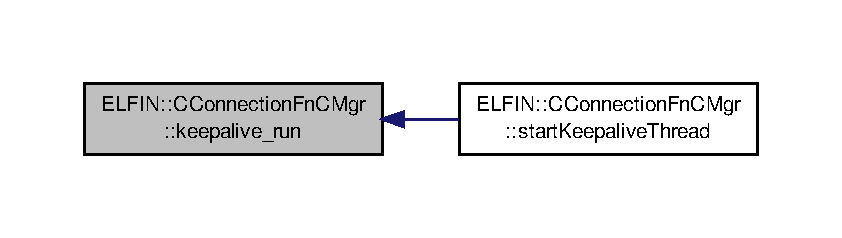
\includegraphics[width=350pt]{class_e_l_f_i_n_1_1_c_connection_fn_c_mgr_a0f4f281ce4e577eb32c8df5052106fa3_icgraph}
\end{center}
\end{figure}


\hypertarget{class_e_l_f_i_n_1_1_c_connection_fn_c_mgr_a59b5a84c9df6d5e706ada67fc32ad0b5}{\index{E\-L\-F\-I\-N\-::\-C\-Connection\-Fn\-C\-Mgr@{E\-L\-F\-I\-N\-::\-C\-Connection\-Fn\-C\-Mgr}!open\-Connection\-To\-Fn\-C@{open\-Connection\-To\-Fn\-C}}
\index{open\-Connection\-To\-Fn\-C@{open\-Connection\-To\-Fn\-C}!ELFIN::CConnectionFnCMgr@{E\-L\-F\-I\-N\-::\-C\-Connection\-Fn\-C\-Mgr}}
\subsubsection[{open\-Connection\-To\-Fn\-C}]{\setlength{\rightskip}{0pt plus 5cm}int E\-L\-F\-I\-N\-::\-C\-Connection\-Fn\-C\-Mgr\-::open\-Connection\-To\-Fn\-C (
\begin{DoxyParamCaption}
\item[{const char $\ast$}]{p\-Reader\-Host\-Name}
\end{DoxyParamCaption}
)\hspace{0.3cm}{\ttfamily [private]}}}\label{class_e_l_f_i_n_1_1_c_connection_fn_c_mgr_a59b5a84c9df6d5e706ada67fc32ad0b5}


Initiate connection to the Fn\-C server (client mode) 



Definition at line 251 of file C\-Connection\-Fn\-C\-Mgr.\-cpp.

\hypertarget{class_e_l_f_i_n_1_1_c_connection_fn_c_mgr_a615454a57231aca62fc6f0fa73df64dd}{\index{E\-L\-F\-I\-N\-::\-C\-Connection\-Fn\-C\-Mgr@{E\-L\-F\-I\-N\-::\-C\-Connection\-Fn\-C\-Mgr}!recv\-Message@{recv\-Message}}
\index{recv\-Message@{recv\-Message}!ELFIN::CConnectionFnCMgr@{E\-L\-F\-I\-N\-::\-C\-Connection\-Fn\-C\-Mgr}}
\subsubsection[{recv\-Message}]{\setlength{\rightskip}{0pt plus 5cm}L\-L\-R\-P\-::\-C\-Message $\ast$ E\-L\-F\-I\-N\-::\-C\-Connection\-Fn\-C\-Mgr\-::recv\-Message (
\begin{DoxyParamCaption}
\item[{int}]{n\-Max\-M\-S}
\end{DoxyParamCaption}
)}}\label{class_e_l_f_i_n_1_1_c_connection_fn_c_mgr_a615454a57231aca62fc6f0fa73df64dd}


Receive the message in recv buffer. 



Definition at line 236 of file C\-Connection\-Fn\-C\-Mgr.\-cpp.

\hypertarget{class_e_l_f_i_n_1_1_c_connection_fn_c_mgr_af7ee83a8a9546bae5c1f83c4f282d56a}{\index{E\-L\-F\-I\-N\-::\-C\-Connection\-Fn\-C\-Mgr@{E\-L\-F\-I\-N\-::\-C\-Connection\-Fn\-C\-Mgr}!send\-Connection\-Attempt\-Event@{send\-Connection\-Attempt\-Event}}
\index{send\-Connection\-Attempt\-Event@{send\-Connection\-Attempt\-Event}!ELFIN::CConnectionFnCMgr@{E\-L\-F\-I\-N\-::\-C\-Connection\-Fn\-C\-Mgr}}
\subsubsection[{send\-Connection\-Attempt\-Event}]{\setlength{\rightskip}{0pt plus 5cm}int E\-L\-F\-I\-N\-::\-C\-Connection\-Fn\-C\-Mgr\-::send\-Connection\-Attempt\-Event (
\begin{DoxyParamCaption}
{}
\end{DoxyParamCaption}
)}}\label{class_e_l_f_i_n_1_1_c_connection_fn_c_mgr_af7ee83a8a9546bae5c1f83c4f282d56a}


Send Connection\-Attempt\-Event notification to the Fn\-C server. 



Definition at line 132 of file C\-Connection\-Fn\-C\-Mgr.\-cpp.



Here is the call graph for this function\-:
\nopagebreak
\begin{figure}[H]
\begin{center}
\leavevmode
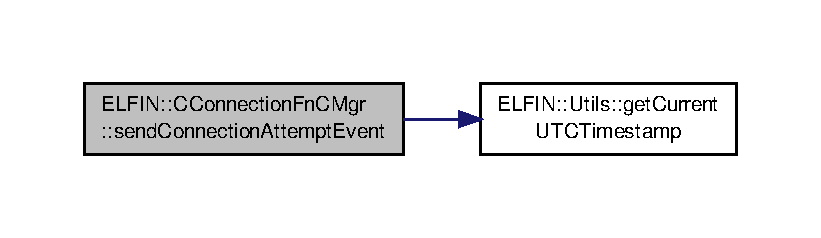
\includegraphics[width=350pt]{class_e_l_f_i_n_1_1_c_connection_fn_c_mgr_af7ee83a8a9546bae5c1f83c4f282d56a_cgraph}
\end{center}
\end{figure}


\hypertarget{class_e_l_f_i_n_1_1_c_connection_fn_c_mgr_a0b5e1d5ffe5b49aef3b52254d443ffef}{\index{E\-L\-F\-I\-N\-::\-C\-Connection\-Fn\-C\-Mgr@{E\-L\-F\-I\-N\-::\-C\-Connection\-Fn\-C\-Mgr}!send\-Connection\-Close\-Event@{send\-Connection\-Close\-Event}}
\index{send\-Connection\-Close\-Event@{send\-Connection\-Close\-Event}!ELFIN::CConnectionFnCMgr@{E\-L\-F\-I\-N\-::\-C\-Connection\-Fn\-C\-Mgr}}
\subsubsection[{send\-Connection\-Close\-Event}]{\setlength{\rightskip}{0pt plus 5cm}int E\-L\-F\-I\-N\-::\-C\-Connection\-Fn\-C\-Mgr\-::send\-Connection\-Close\-Event (
\begin{DoxyParamCaption}
{}
\end{DoxyParamCaption}
)}}\label{class_e_l_f_i_n_1_1_c_connection_fn_c_mgr_a0b5e1d5ffe5b49aef3b52254d443ffef}


Send Connection\-Close\-Event notification to the Fn\-C server. 



Definition at line 185 of file C\-Connection\-Fn\-C\-Mgr.\-cpp.



Here is the call graph for this function\-:
\nopagebreak
\begin{figure}[H]
\begin{center}
\leavevmode
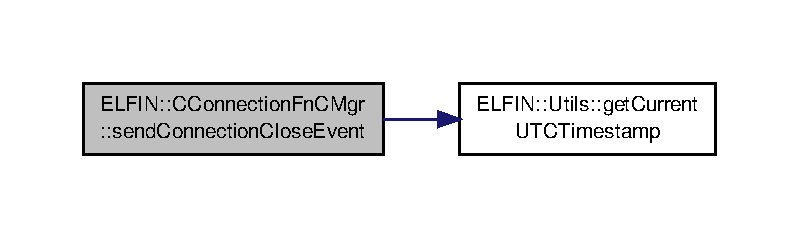
\includegraphics[width=350pt]{class_e_l_f_i_n_1_1_c_connection_fn_c_mgr_a0b5e1d5ffe5b49aef3b52254d443ffef_cgraph}
\end{center}
\end{figure}


\hypertarget{class_e_l_f_i_n_1_1_c_connection_fn_c_mgr_a48b283f30ddd8c2b0c2ed55e844085f8}{\index{E\-L\-F\-I\-N\-::\-C\-Connection\-Fn\-C\-Mgr@{E\-L\-F\-I\-N\-::\-C\-Connection\-Fn\-C\-Mgr}!send\-Message@{send\-Message}}
\index{send\-Message@{send\-Message}!ELFIN::CConnectionFnCMgr@{E\-L\-F\-I\-N\-::\-C\-Connection\-Fn\-C\-Mgr}}
\subsubsection[{send\-Message}]{\setlength{\rightskip}{0pt plus 5cm}int E\-L\-F\-I\-N\-::\-C\-Connection\-Fn\-C\-Mgr\-::send\-Message (
\begin{DoxyParamCaption}
\item[{L\-L\-R\-P\-::\-C\-Message $\ast$}]{p\-Message}
\end{DoxyParamCaption}
)}}\label{class_e_l_f_i_n_1_1_c_connection_fn_c_mgr_a48b283f30ddd8c2b0c2ed55e844085f8}


Queue the message to send buffer. 



Definition at line 264 of file C\-Connection\-Fn\-C\-Mgr.\-cpp.

\hypertarget{class_e_l_f_i_n_1_1_c_connection_fn_c_mgr_a248b1ad1d6138f5ade40892f3afb5a68}{\index{E\-L\-F\-I\-N\-::\-C\-Connection\-Fn\-C\-Mgr@{E\-L\-F\-I\-N\-::\-C\-Connection\-Fn\-C\-Mgr}!set\-Received\-Keepalive\-Id@{set\-Received\-Keepalive\-Id}}
\index{set\-Received\-Keepalive\-Id@{set\-Received\-Keepalive\-Id}!ELFIN::CConnectionFnCMgr@{E\-L\-F\-I\-N\-::\-C\-Connection\-Fn\-C\-Mgr}}
\subsubsection[{set\-Received\-Keepalive\-Id}]{\setlength{\rightskip}{0pt plus 5cm}void E\-L\-F\-I\-N\-::\-C\-Connection\-Fn\-C\-Mgr\-::set\-Received\-Keepalive\-Id (
\begin{DoxyParamCaption}
\item[{int}]{\-\_\-\-\_\-received\-Keepalive\-I\-D}
\end{DoxyParamCaption}
)}}\label{class_e_l_f_i_n_1_1_c_connection_fn_c_mgr_a248b1ad1d6138f5ade40892f3afb5a68}


Set the \-\_\-received\-Keepalive\-I\-D id with given id. 



Definition at line 321 of file C\-Connection\-Fn\-C\-Mgr.\-cpp.

\hypertarget{class_e_l_f_i_n_1_1_c_connection_fn_c_mgr_afeb7e321253ac8ab298958393ecfabc5}{\index{E\-L\-F\-I\-N\-::\-C\-Connection\-Fn\-C\-Mgr@{E\-L\-F\-I\-N\-::\-C\-Connection\-Fn\-C\-Mgr}!start\-Connection@{start\-Connection}}
\index{start\-Connection@{start\-Connection}!ELFIN::CConnectionFnCMgr@{E\-L\-F\-I\-N\-::\-C\-Connection\-Fn\-C\-Mgr}}
\subsubsection[{start\-Connection}]{\setlength{\rightskip}{0pt plus 5cm}int E\-L\-F\-I\-N\-::\-C\-Connection\-Fn\-C\-Mgr\-::start\-Connection (
\begin{DoxyParamCaption}
\item[{{\bf Program\-Options} $\ast$}]{\-\_\-\-\_\-prog\-Opt}
\end{DoxyParamCaption}
)}}\label{class_e_l_f_i_n_1_1_c_connection_fn_c_mgr_afeb7e321253ac8ab298958393ecfabc5}


Start connection to the Fn\-C server. Checks reader\-\_\-initiated option to decide whether to initiate connection or wait for connection. 



Definition at line 50 of file C\-Connection\-Fn\-C\-Mgr.\-cpp.



Here is the call graph for this function\-:
\nopagebreak
\begin{figure}[H]
\begin{center}
\leavevmode
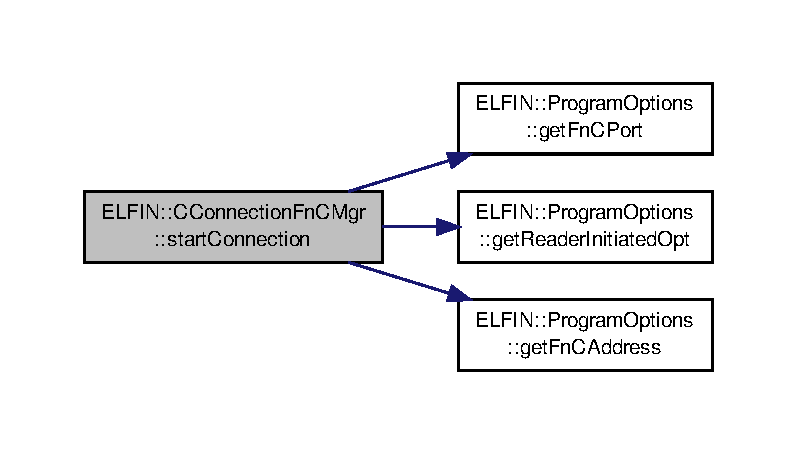
\includegraphics[width=350pt]{class_e_l_f_i_n_1_1_c_connection_fn_c_mgr_afeb7e321253ac8ab298958393ecfabc5_cgraph}
\end{center}
\end{figure}


\hypertarget{class_e_l_f_i_n_1_1_c_connection_fn_c_mgr_a0c54ce49b3d0c1219f30b89a77062493}{\index{E\-L\-F\-I\-N\-::\-C\-Connection\-Fn\-C\-Mgr@{E\-L\-F\-I\-N\-::\-C\-Connection\-Fn\-C\-Mgr}!start\-Keepalive\-Thread@{start\-Keepalive\-Thread}}
\index{start\-Keepalive\-Thread@{start\-Keepalive\-Thread}!ELFIN::CConnectionFnCMgr@{E\-L\-F\-I\-N\-::\-C\-Connection\-Fn\-C\-Mgr}}
\subsubsection[{start\-Keepalive\-Thread}]{\setlength{\rightskip}{0pt plus 5cm}int E\-L\-F\-I\-N\-::\-C\-Connection\-Fn\-C\-Mgr\-::start\-Keepalive\-Thread (
\begin{DoxyParamCaption}
\item[{int}]{period\-M\-S}
\end{DoxyParamCaption}
)}}\label{class_e_l_f_i_n_1_1_c_connection_fn_c_mgr_a0c54ce49b3d0c1219f30b89a77062493}


Create the keepalive thread. 



Definition at line 327 of file C\-Connection\-Fn\-C\-Mgr.\-cpp.



Here is the call graph for this function\-:
\nopagebreak
\begin{figure}[H]
\begin{center}
\leavevmode
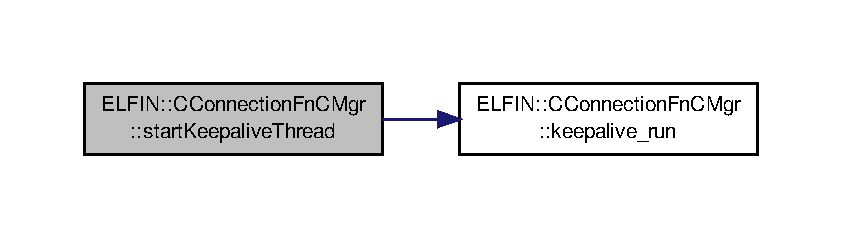
\includegraphics[width=350pt]{class_e_l_f_i_n_1_1_c_connection_fn_c_mgr_a0c54ce49b3d0c1219f30b89a77062493_cgraph}
\end{center}
\end{figure}


\hypertarget{class_e_l_f_i_n_1_1_c_connection_fn_c_mgr_aa23c373881a560ef974cd1152ea76c43}{\index{E\-L\-F\-I\-N\-::\-C\-Connection\-Fn\-C\-Mgr@{E\-L\-F\-I\-N\-::\-C\-Connection\-Fn\-C\-Mgr}!stop\-Keepalive\-Thread@{stop\-Keepalive\-Thread}}
\index{stop\-Keepalive\-Thread@{stop\-Keepalive\-Thread}!ELFIN::CConnectionFnCMgr@{E\-L\-F\-I\-N\-::\-C\-Connection\-Fn\-C\-Mgr}}
\subsubsection[{stop\-Keepalive\-Thread}]{\setlength{\rightskip}{0pt plus 5cm}int E\-L\-F\-I\-N\-::\-C\-Connection\-Fn\-C\-Mgr\-::stop\-Keepalive\-Thread (
\begin{DoxyParamCaption}
{}
\end{DoxyParamCaption}
)}}\label{class_e_l_f_i_n_1_1_c_connection_fn_c_mgr_aa23c373881a560ef974cd1152ea76c43}


Interrupt and stop the keepalive thread. 



Definition at line 341 of file C\-Connection\-Fn\-C\-Mgr.\-cpp.

\hypertarget{class_e_l_f_i_n_1_1_c_connection_fn_c_mgr_af86142cdff404912079d5b48883378ad}{\index{E\-L\-F\-I\-N\-::\-C\-Connection\-Fn\-C\-Mgr@{E\-L\-F\-I\-N\-::\-C\-Connection\-Fn\-C\-Mgr}!wait\-For\-Connection@{wait\-For\-Connection}}
\index{wait\-For\-Connection@{wait\-For\-Connection}!ELFIN::CConnectionFnCMgr@{E\-L\-F\-I\-N\-::\-C\-Connection\-Fn\-C\-Mgr}}
\subsubsection[{wait\-For\-Connection}]{\setlength{\rightskip}{0pt plus 5cm}int E\-L\-F\-I\-N\-::\-C\-Connection\-Fn\-C\-Mgr\-::wait\-For\-Connection (
\begin{DoxyParamCaption}
{}
\end{DoxyParamCaption}
)\hspace{0.3cm}{\ttfamily [private]}}}\label{class_e_l_f_i_n_1_1_c_connection_fn_c_mgr_af86142cdff404912079d5b48883378ad}


Wait for connection from the Fn\-C server (server mode) 



Definition at line 117 of file C\-Connection\-Fn\-C\-Mgr.\-cpp.



The documentation for this class was generated from the following files\-:\begin{DoxyCompactItemize}
\item 
elfin\-\_\-src/\hyperlink{_c_connection_fn_c_mgr_8h}{C\-Connection\-Fn\-C\-Mgr.\-h}\item 
elfin\-\_\-src/\hyperlink{_c_connection_fn_c_mgr_8cpp}{C\-Connection\-Fn\-C\-Mgr.\-cpp}\end{DoxyCompactItemize}

\hypertarget{class_e_l_f_i_n_1_1_e_l_f_i_n_reader}{\section{E\-L\-F\-I\-N\-:\-:E\-L\-F\-I\-N\-Reader Class Reference}
\label{class_e_l_f_i_n_1_1_e_l_f_i_n_reader}\index{E\-L\-F\-I\-N\-::\-E\-L\-F\-I\-N\-Reader@{E\-L\-F\-I\-N\-::\-E\-L\-F\-I\-N\-Reader}}
}


Collaboration diagram for E\-L\-F\-I\-N\-:\-:E\-L\-F\-I\-N\-Reader\-:
\nopagebreak
\begin{figure}[H]
\begin{center}
\leavevmode
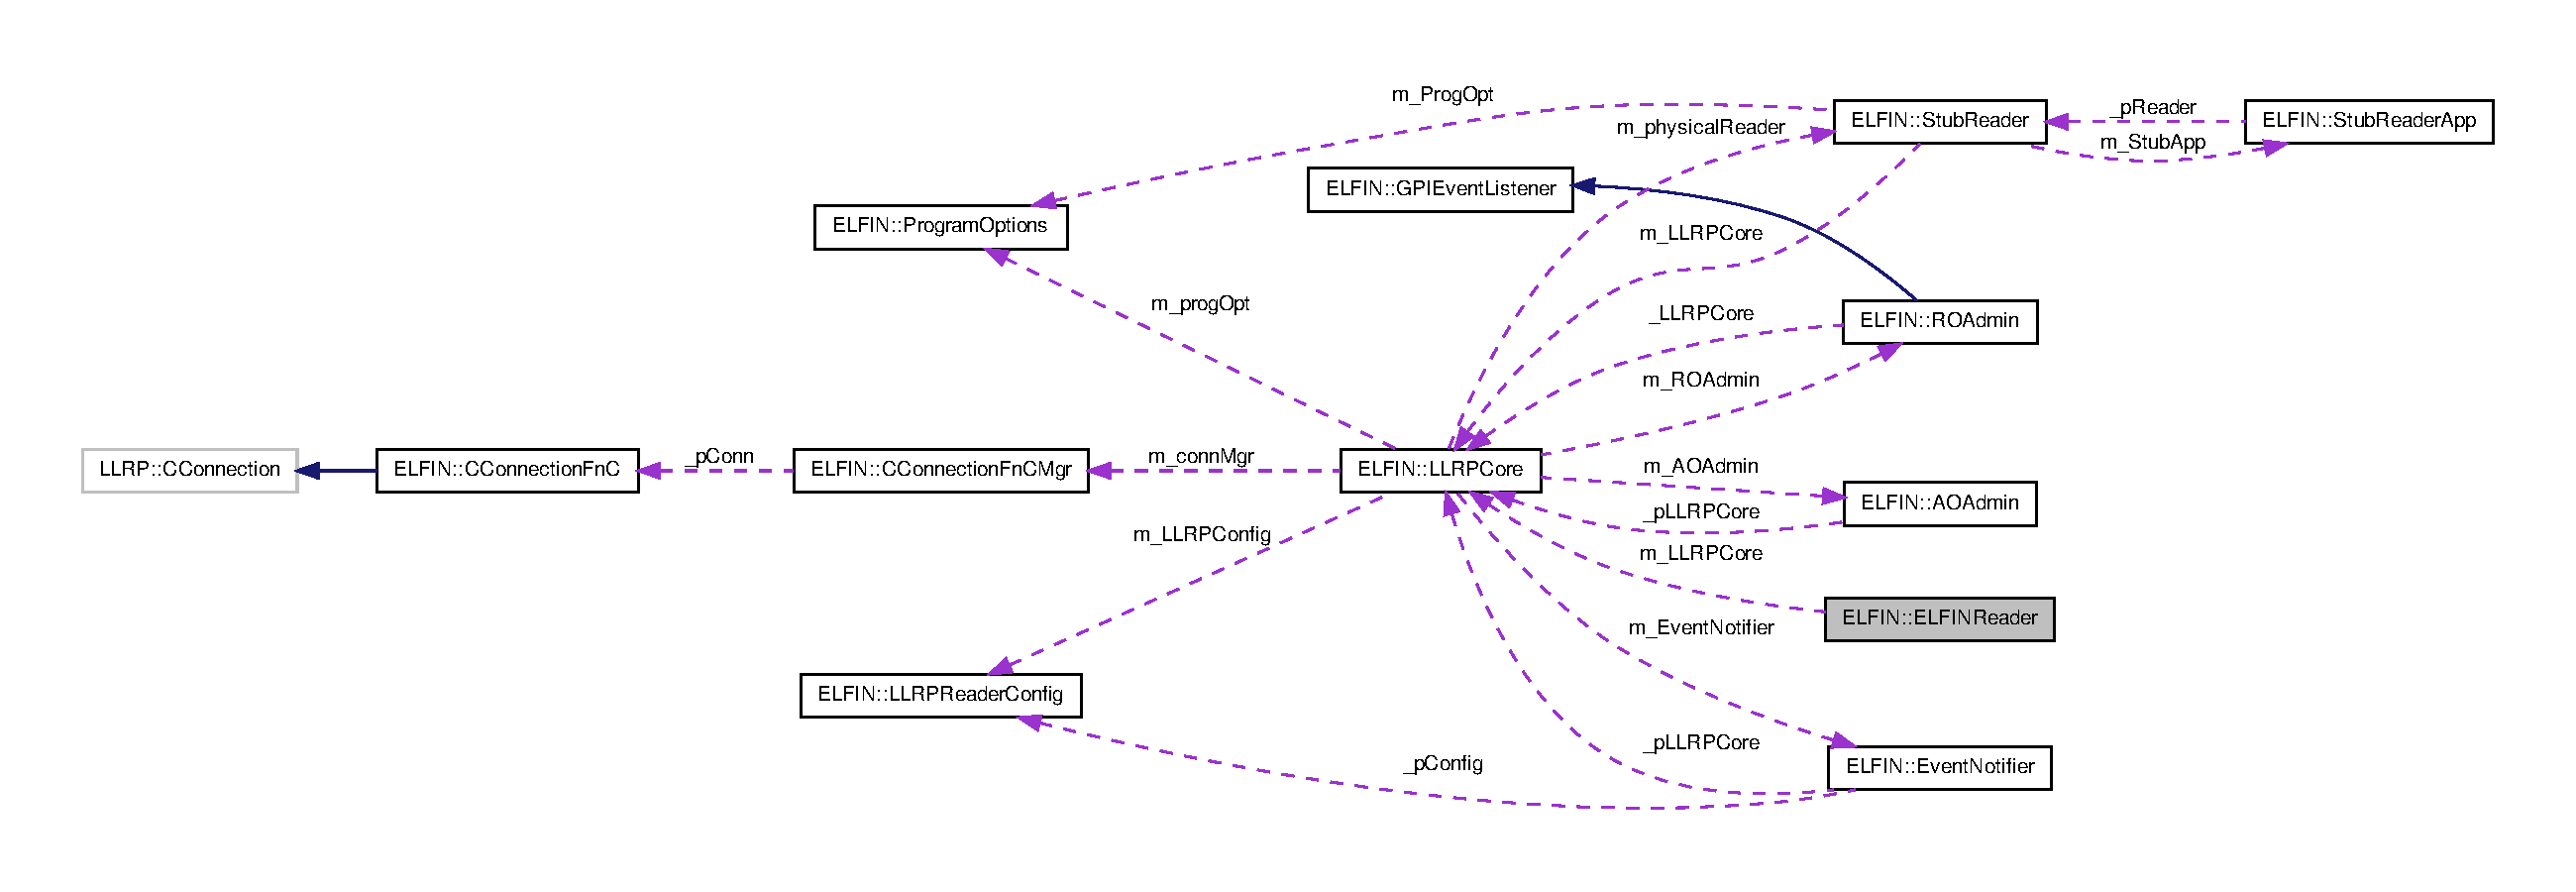
\includegraphics[width=350pt]{class_e_l_f_i_n_1_1_e_l_f_i_n_reader__coll__graph}
\end{center}
\end{figure}
\subsection*{Public Member Functions}
\begin{DoxyCompactItemize}
\item 
\hypertarget{class_e_l_f_i_n_1_1_e_l_f_i_n_reader_a6761951572d8ba5bef6c89f3c88b4c30}{{\bfseries E\-L\-F\-I\-N\-Reader} (\hyperlink{class_e_l_f_i_n_1_1_program_options}{Program\-Options} $\ast$\-\_\-\-\_\-prog\-Opt)}\label{class_e_l_f_i_n_1_1_e_l_f_i_n_reader_a6761951572d8ba5bef6c89f3c88b4c30}

\item 
\hypertarget{class_e_l_f_i_n_1_1_e_l_f_i_n_reader_ac4a16aee0b03a1859644bc9810d7cc5c}{int {\bfseries run} ()}\label{class_e_l_f_i_n_1_1_e_l_f_i_n_reader_ac4a16aee0b03a1859644bc9810d7cc5c}

\item 
\hypertarget{class_e_l_f_i_n_1_1_e_l_f_i_n_reader_ad6daa88daa3d64a27718dc6080bd8e38}{int {\bfseries init} ()}\label{class_e_l_f_i_n_1_1_e_l_f_i_n_reader_ad6daa88daa3d64a27718dc6080bd8e38}

\item 
\hypertarget{class_e_l_f_i_n_1_1_e_l_f_i_n_reader_afe07fe488fe3518f166b9dd825c7ae50}{int {\bfseries connect\-Reader\-App} (\hyperlink{class_e_l_f_i_n_1_1_stub_reader_app}{Stub\-Reader\-App} $\ast$\-\_\-reader\-App)}\label{class_e_l_f_i_n_1_1_e_l_f_i_n_reader_afe07fe488fe3518f166b9dd825c7ae50}

\item 
\hypertarget{class_e_l_f_i_n_1_1_e_l_f_i_n_reader_a8ad1b68f18ed7a9412ddd5b04e08bf8d}{void {\bfseries set\-Shutdown\-Flag} ()}\label{class_e_l_f_i_n_1_1_e_l_f_i_n_reader_a8ad1b68f18ed7a9412ddd5b04e08bf8d}

\item 
\hypertarget{class_e_l_f_i_n_1_1_e_l_f_i_n_reader_a7427c1f4bfc8374aa564de45feac9f9d}{int {\bfseries get\-Shutdown\-Flag} ()}\label{class_e_l_f_i_n_1_1_e_l_f_i_n_reader_a7427c1f4bfc8374aa564de45feac9f9d}

\item 
\hypertarget{class_e_l_f_i_n_1_1_e_l_f_i_n_reader_a878736b02c826041f149137069967cef}{int {\bfseries start\-Connection} ()}\label{class_e_l_f_i_n_1_1_e_l_f_i_n_reader_a878736b02c826041f149137069967cef}

\end{DoxyCompactItemize}
\subsection*{Private Attributes}
\begin{DoxyCompactItemize}
\item 
\hypertarget{class_e_l_f_i_n_1_1_e_l_f_i_n_reader_ad8dce6f480b4c750291057ae842e28d6}{\hyperlink{class_e_l_f_i_n_1_1_l_l_r_p_core}{L\-L\-R\-P\-Core} $\ast$ {\bfseries m\-\_\-\-L\-L\-R\-P\-Core}}\label{class_e_l_f_i_n_1_1_e_l_f_i_n_reader_ad8dce6f480b4c750291057ae842e28d6}

\end{DoxyCompactItemize}


\subsection{Detailed Description}


Definition at line 17 of file E\-L\-F\-I\-N\-Reader.\-h.



The documentation for this class was generated from the following files\-:\begin{DoxyCompactItemize}
\item 
elfin\-\_\-src/E\-L\-F\-I\-N\-Reader.\-h\item 
elfin\-\_\-src/E\-L\-F\-I\-N\-Reader.\-cpp\end{DoxyCompactItemize}

\hypertarget{class_e_l_f_i_n_1_1_event_notifier}{\section{E\-L\-F\-I\-N\-:\-:Event\-Notifier Class Reference}
\label{class_e_l_f_i_n_1_1_event_notifier}\index{E\-L\-F\-I\-N\-::\-Event\-Notifier@{E\-L\-F\-I\-N\-::\-Event\-Notifier}}
}


Create and send Reader\-Event\-Notifications to the Fn\-C server.  




{\ttfamily \#include $<$Event\-Notifier.\-h$>$}



Collaboration diagram for E\-L\-F\-I\-N\-:\-:Event\-Notifier\-:
\nopagebreak
\begin{figure}[H]
\begin{center}
\leavevmode
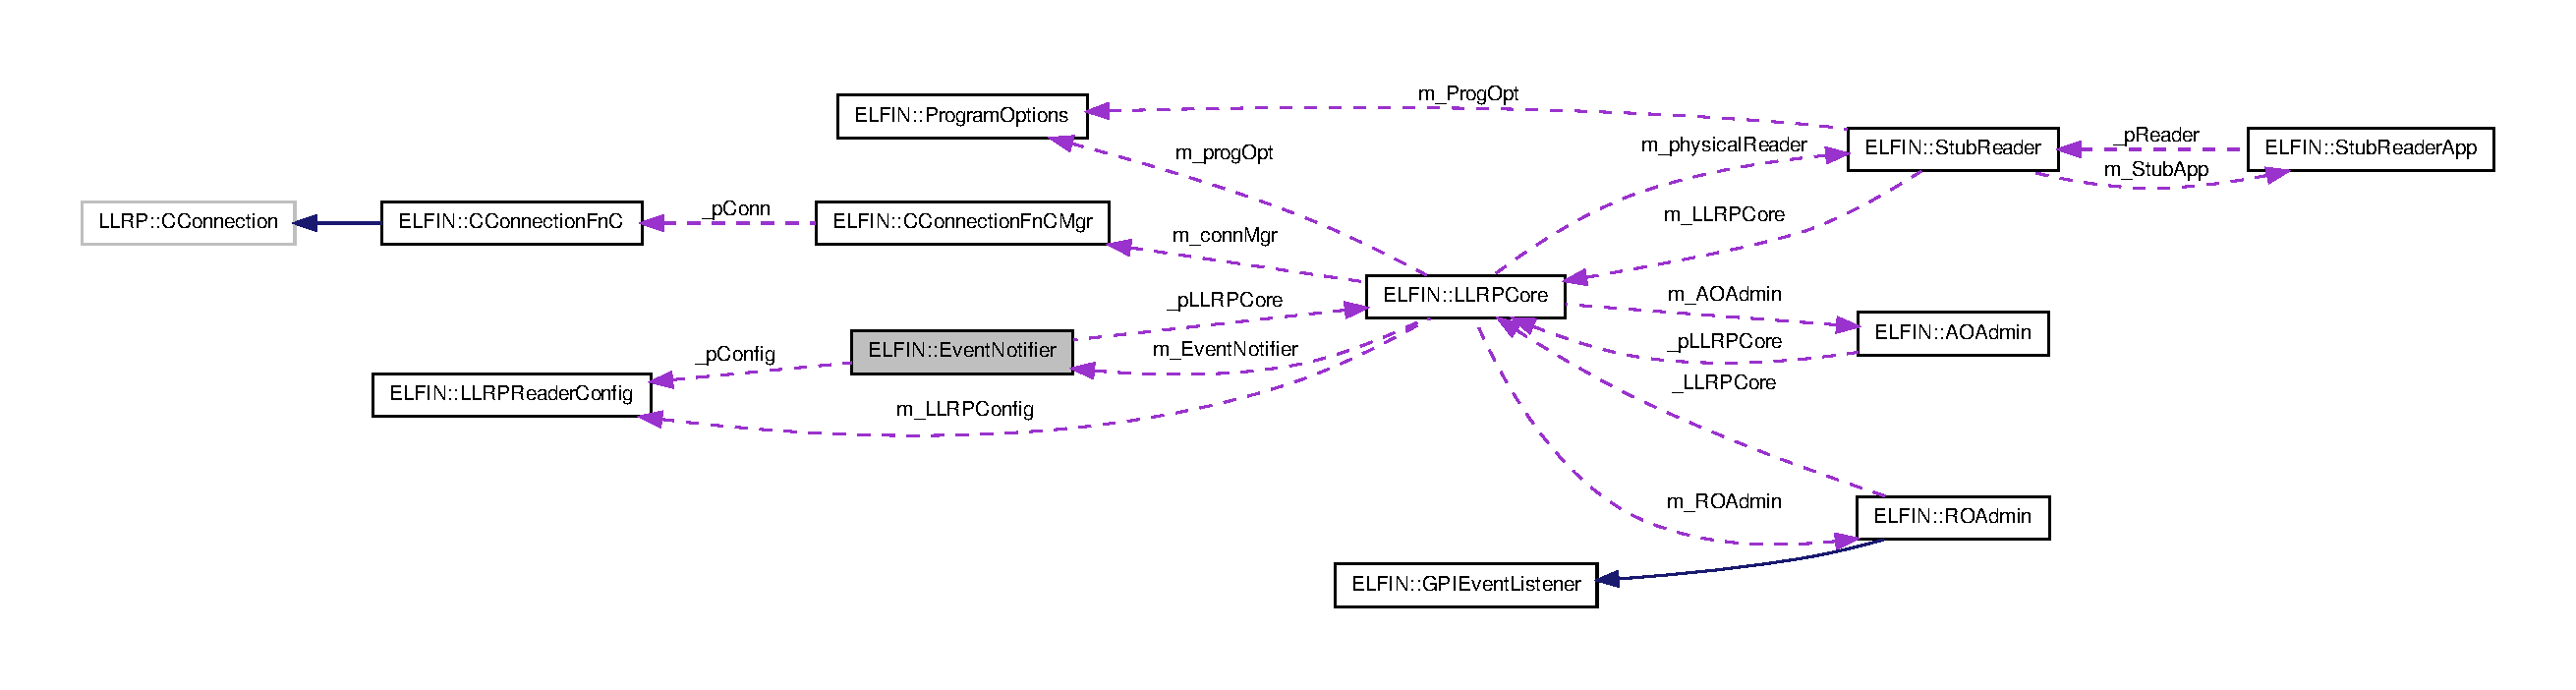
\includegraphics[width=350pt]{class_e_l_f_i_n_1_1_event_notifier__coll__graph}
\end{center}
\end{figure}
\subsection*{Public Member Functions}
\begin{DoxyCompactItemize}
\item 
\hyperlink{class_e_l_f_i_n_1_1_event_notifier_a8dbb404de4d2428b4d1c56c941318d27}{Event\-Notifier} (\hyperlink{class_e_l_f_i_n_1_1_l_l_r_p_core}{L\-L\-R\-P\-Core} $\ast$\-\_\-\-\_\-p\-L\-L\-R\-P\-Core)
\begin{DoxyCompactList}\small\item\em Constructor of \hyperlink{class_e_l_f_i_n_1_1_event_notifier}{Event\-Notifier} class. \end{DoxyCompactList}\item 
\hyperlink{class_e_l_f_i_n_1_1_event_notifier_a04ffb92dce7ddb26097dcce5546c9aae}{$\sim$\-Event\-Notifier} ()
\begin{DoxyCompactList}\small\item\em Destructor of \hyperlink{class_e_l_f_i_n_1_1_event_notifier}{Event\-Notifier} class. \end{DoxyCompactList}\end{DoxyCompactItemize}
{\bf }\par
\begin{DoxyCompactItemize}
\item 
int \hyperlink{class_e_l_f_i_n_1_1_event_notifier_a87bfe980b95821a36877e3943d272c84}{send\-G\-P\-I\-Event} (L\-L\-R\-P\-::llrp\-\_\-u32\-\_\-t G\-P\-I\-Port\-Number, L\-L\-R\-P\-::llrp\-\_\-u32\-\_\-t G\-P\-I\-Event)
\begin{DoxyCompactList}\small\item\em Send corresponding event, if that event notification is enabled. \end{DoxyCompactList}\item 
int \hyperlink{class_e_l_f_i_n_1_1_event_notifier_a3cf83b4e23b8c16fa587e25391dc968b}{send\-R\-O\-Spec\-Event} (L\-L\-R\-P\-::llrp\-\_\-u32\-\_\-t R\-O\-Spec\-I\-D, enum L\-L\-R\-P\-::\-E\-R\-O\-Spec\-Event\-Type Event\-Type, L\-L\-R\-P\-::llrp\-\_\-u32\-\_\-t Preemting\-R\-O\-Spec\-I\-D)
\begin{DoxyCompactList}\small\item\em Send corresponding event, if that event notification is enabled. \end{DoxyCompactList}\item 
int \hyperlink{class_e_l_f_i_n_1_1_event_notifier_a6526cc3f783409969343a5065efbf22d}{send\-A\-I\-Spec\-Event} (L\-L\-R\-P\-::llrp\-\_\-u32\-\_\-t R\-O\-Spec\-I\-D, L\-L\-R\-P\-::llrp\-\_\-u16\-\_\-t Spec\-Index, enum L\-L\-R\-P\-::\-E\-A\-I\-Spec\-Event\-Type Event\-Type)
\begin{DoxyCompactList}\small\item\em Send corresponding event, if that event notification is enabled. \end{DoxyCompactList}\item 
int \hyperlink{class_e_l_f_i_n_1_1_event_notifier_a70cc63c7ff09a5ed43e3e8315de34c4f}{send\-Connection\-Attempt\-Event} (enum L\-L\-R\-P\-::\-E\-Connection\-Attempt\-Status\-Type Event\-Type)
\begin{DoxyCompactList}\small\item\em Send corresponding event, if that event notification is enabled. \end{DoxyCompactList}\item 
int \hyperlink{class_e_l_f_i_n_1_1_event_notifier_a82b6fdfe8cf4429e4b0624a0421ddbf2}{sedn\-Connection\-Close\-Event} ()
\begin{DoxyCompactList}\small\item\em Send corresponding event, if that event notification is enabled. \end{DoxyCompactList}\item 
int \hyperlink{class_e_l_f_i_n_1_1_event_notifier_a667910f5c8ea77f2a30f989c1feaea31}{send\-Spec\-Loop\-Event} (L\-L\-R\-P\-::llrp\-\_\-u32\-\_\-t R\-O\-Spec\-I\-D, L\-L\-R\-P\-::llrp\-\_\-u32\-\_\-t Loop\-Count)
\begin{DoxyCompactList}\small\item\em Send corresponding event, if that event notification is enabled. \end{DoxyCompactList}\end{DoxyCompactItemize}

{\bf }\par
\begin{DoxyCompactItemize}
\item 
int \hyperlink{class_e_l_f_i_n_1_1_event_notifier_a03d74a6b19765174ad05013f8f0e51d4}{send\-Hopping\-Event} (int Hop\-Table\-I\-D, int Next\-Channel\-Index)
\begin{DoxyCompactList}\small\item\em These events are not implemented, because they are optional. \end{DoxyCompactList}\item 
int \hyperlink{class_e_l_f_i_n_1_1_event_notifier_ab1aa4c5e86335d17c6e091b49d8979a8}{send\-Report\-Buffer\-Level\-Warning\-Event} (int Report\-Buffer\-Percentage\-Full)
\begin{DoxyCompactList}\small\item\em These events are not implemented, because they are optional. \end{DoxyCompactList}\item 
int \hyperlink{class_e_l_f_i_n_1_1_event_notifier_af1beb53b55e0ef06fc5711d86abe7e61}{send\-Report\-Buffer\-Overflow\-Error\-Event} ()
\begin{DoxyCompactList}\small\item\em These events are not implemented, because they are optional. \end{DoxyCompactList}\item 
int \hyperlink{class_e_l_f_i_n_1_1_event_notifier_a756c170fc8e5de0e1ae1c53e69efa833}{send\-Reader\-Exception\-Event} ()
\begin{DoxyCompactList}\small\item\em These events are not implemented, because they are optional. \end{DoxyCompactList}\item 
int \hyperlink{class_e_l_f_i_n_1_1_event_notifier_a7a618ade6fbf12cb93ec11fef5b396cd}{send\-R\-F\-Survey\-Event} (int R\-O\-Spec\-I\-D, int Spec\-Index, enum L\-L\-R\-P\-::\-E\-R\-F\-Survey\-Event\-Type Event\-Type)
\begin{DoxyCompactList}\small\item\em These events are not implemented, because they are optional. \end{DoxyCompactList}\item 
int \hyperlink{class_e_l_f_i_n_1_1_event_notifier_a5f5c26ba9f40ea6cc9b0f166bdfaca8d}{send\-Antenna\-Event} (int Antenna\-I\-D, enum L\-L\-R\-P\-::\-E\-Antenna\-Event\-Type Event\-Type)
\begin{DoxyCompactList}\small\item\em These events are not implemented, because they are optional. \end{DoxyCompactList}\end{DoxyCompactItemize}

\subsection*{Private Attributes}
\begin{DoxyCompactItemize}
\item 
\hypertarget{class_e_l_f_i_n_1_1_event_notifier_ab9f5bee1cc10452b1accfd726acea89d}{\hyperlink{class_e_l_f_i_n_1_1_l_l_r_p_core}{L\-L\-R\-P\-Core} $\ast$ {\bfseries \-\_\-p\-L\-L\-R\-P\-Core}}\label{class_e_l_f_i_n_1_1_event_notifier_ab9f5bee1cc10452b1accfd726acea89d}

\item 
\hypertarget{class_e_l_f_i_n_1_1_event_notifier_a021bf479e1090a3e7daf403a34fcfefa}{\hyperlink{class_e_l_f_i_n_1_1_l_l_r_p_reader_config}{L\-L\-R\-P\-Reader\-Config} $\ast$ {\bfseries \-\_\-p\-Config}}\label{class_e_l_f_i_n_1_1_event_notifier_a021bf479e1090a3e7daf403a34fcfefa}

\end{DoxyCompactItemize}


\subsection{Detailed Description}
Create and send Reader\-Event\-Notifications to the Fn\-C server. 

\begin{DoxyRemark}{Remarks}
Event methods of this class can be just called where the event should be sent, because each method checks whether the corresponding event is enabled or not before sending it. 
\end{DoxyRemark}


Definition at line 27 of file Event\-Notifier.\-h.



\subsection{Constructor \& Destructor Documentation}
\hypertarget{class_e_l_f_i_n_1_1_event_notifier_a8dbb404de4d2428b4d1c56c941318d27}{\index{E\-L\-F\-I\-N\-::\-Event\-Notifier@{E\-L\-F\-I\-N\-::\-Event\-Notifier}!Event\-Notifier@{Event\-Notifier}}
\index{Event\-Notifier@{Event\-Notifier}!ELFIN::EventNotifier@{E\-L\-F\-I\-N\-::\-Event\-Notifier}}
\subsubsection[{Event\-Notifier}]{\setlength{\rightskip}{0pt plus 5cm}E\-L\-F\-I\-N\-::\-Event\-Notifier\-::\-Event\-Notifier (
\begin{DoxyParamCaption}
\item[{{\bf L\-L\-R\-P\-Core} $\ast$}]{\-\_\-\-\_\-p\-L\-L\-R\-P\-Core}
\end{DoxyParamCaption}
)}}\label{class_e_l_f_i_n_1_1_event_notifier_a8dbb404de4d2428b4d1c56c941318d27}


Constructor of \hyperlink{class_e_l_f_i_n_1_1_event_notifier}{Event\-Notifier} class. 



Definition at line 11 of file Event\-Notifier.\-cpp.

\hypertarget{class_e_l_f_i_n_1_1_event_notifier_a04ffb92dce7ddb26097dcce5546c9aae}{\index{E\-L\-F\-I\-N\-::\-Event\-Notifier@{E\-L\-F\-I\-N\-::\-Event\-Notifier}!$\sim$\-Event\-Notifier@{$\sim$\-Event\-Notifier}}
\index{$\sim$\-Event\-Notifier@{$\sim$\-Event\-Notifier}!ELFIN::EventNotifier@{E\-L\-F\-I\-N\-::\-Event\-Notifier}}
\subsubsection[{$\sim$\-Event\-Notifier}]{\setlength{\rightskip}{0pt plus 5cm}E\-L\-F\-I\-N\-::\-Event\-Notifier\-::$\sim$\-Event\-Notifier (
\begin{DoxyParamCaption}
{}
\end{DoxyParamCaption}
)}}\label{class_e_l_f_i_n_1_1_event_notifier_a04ffb92dce7ddb26097dcce5546c9aae}


Destructor of \hyperlink{class_e_l_f_i_n_1_1_event_notifier}{Event\-Notifier} class. 



Definition at line 16 of file Event\-Notifier.\-cpp.



\subsection{Member Function Documentation}
\hypertarget{class_e_l_f_i_n_1_1_event_notifier_a82b6fdfe8cf4429e4b0624a0421ddbf2}{\index{E\-L\-F\-I\-N\-::\-Event\-Notifier@{E\-L\-F\-I\-N\-::\-Event\-Notifier}!sedn\-Connection\-Close\-Event@{sedn\-Connection\-Close\-Event}}
\index{sedn\-Connection\-Close\-Event@{sedn\-Connection\-Close\-Event}!ELFIN::EventNotifier@{E\-L\-F\-I\-N\-::\-Event\-Notifier}}
\subsubsection[{sedn\-Connection\-Close\-Event}]{\setlength{\rightskip}{0pt plus 5cm}int E\-L\-F\-I\-N\-::\-Event\-Notifier\-::sedn\-Connection\-Close\-Event (
\begin{DoxyParamCaption}
{}
\end{DoxyParamCaption}
)}}\label{class_e_l_f_i_n_1_1_event_notifier_a82b6fdfe8cf4429e4b0624a0421ddbf2}


Send corresponding event, if that event notification is enabled. 



Definition at line 51 of file Event\-Notifier.\-cpp.

\hypertarget{class_e_l_f_i_n_1_1_event_notifier_a6526cc3f783409969343a5065efbf22d}{\index{E\-L\-F\-I\-N\-::\-Event\-Notifier@{E\-L\-F\-I\-N\-::\-Event\-Notifier}!send\-A\-I\-Spec\-Event@{send\-A\-I\-Spec\-Event}}
\index{send\-A\-I\-Spec\-Event@{send\-A\-I\-Spec\-Event}!ELFIN::EventNotifier@{E\-L\-F\-I\-N\-::\-Event\-Notifier}}
\subsubsection[{send\-A\-I\-Spec\-Event}]{\setlength{\rightskip}{0pt plus 5cm}int E\-L\-F\-I\-N\-::\-Event\-Notifier\-::send\-A\-I\-Spec\-Event (
\begin{DoxyParamCaption}
\item[{L\-L\-R\-P\-::llrp\-\_\-u32\-\_\-t}]{R\-O\-Spec\-I\-D, }
\item[{L\-L\-R\-P\-::llrp\-\_\-u16\-\_\-t}]{Spec\-Index, }
\item[{enum L\-L\-R\-P\-::\-E\-A\-I\-Spec\-Event\-Type}]{Event\-Type}
\end{DoxyParamCaption}
)}}\label{class_e_l_f_i_n_1_1_event_notifier_a6526cc3f783409969343a5065efbf22d}


Send corresponding event, if that event notification is enabled. 



Definition at line 78 of file Event\-Notifier.\-cpp.



Here is the call graph for this function\-:
\nopagebreak
\begin{figure}[H]
\begin{center}
\leavevmode
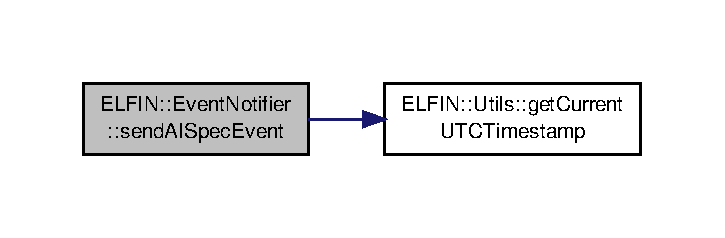
\includegraphics[width=348pt]{class_e_l_f_i_n_1_1_event_notifier_a6526cc3f783409969343a5065efbf22d_cgraph}
\end{center}
\end{figure}


\hypertarget{class_e_l_f_i_n_1_1_event_notifier_a5f5c26ba9f40ea6cc9b0f166bdfaca8d}{\index{E\-L\-F\-I\-N\-::\-Event\-Notifier@{E\-L\-F\-I\-N\-::\-Event\-Notifier}!send\-Antenna\-Event@{send\-Antenna\-Event}}
\index{send\-Antenna\-Event@{send\-Antenna\-Event}!ELFIN::EventNotifier@{E\-L\-F\-I\-N\-::\-Event\-Notifier}}
\subsubsection[{send\-Antenna\-Event}]{\setlength{\rightskip}{0pt plus 5cm}int E\-L\-F\-I\-N\-::\-Event\-Notifier\-::send\-Antenna\-Event (
\begin{DoxyParamCaption}
\item[{int}]{Antenna\-I\-D, }
\item[{enum L\-L\-R\-P\-::\-E\-Antenna\-Event\-Type}]{Event\-Type}
\end{DoxyParamCaption}
)}}\label{class_e_l_f_i_n_1_1_event_notifier_a5f5c26ba9f40ea6cc9b0f166bdfaca8d}


These events are not implemented, because they are optional. 



Definition at line 100 of file Event\-Notifier.\-cpp.

\hypertarget{class_e_l_f_i_n_1_1_event_notifier_a70cc63c7ff09a5ed43e3e8315de34c4f}{\index{E\-L\-F\-I\-N\-::\-Event\-Notifier@{E\-L\-F\-I\-N\-::\-Event\-Notifier}!send\-Connection\-Attempt\-Event@{send\-Connection\-Attempt\-Event}}
\index{send\-Connection\-Attempt\-Event@{send\-Connection\-Attempt\-Event}!ELFIN::EventNotifier@{E\-L\-F\-I\-N\-::\-Event\-Notifier}}
\subsubsection[{send\-Connection\-Attempt\-Event}]{\setlength{\rightskip}{0pt plus 5cm}int E\-L\-F\-I\-N\-::\-Event\-Notifier\-::send\-Connection\-Attempt\-Event (
\begin{DoxyParamCaption}
\item[{enum L\-L\-R\-P\-::\-E\-Connection\-Attempt\-Status\-Type}]{Event\-Type}
\end{DoxyParamCaption}
)}}\label{class_e_l_f_i_n_1_1_event_notifier_a70cc63c7ff09a5ed43e3e8315de34c4f}


Send corresponding event, if that event notification is enabled. 



Definition at line 46 of file Event\-Notifier.\-cpp.

\hypertarget{class_e_l_f_i_n_1_1_event_notifier_a87bfe980b95821a36877e3943d272c84}{\index{E\-L\-F\-I\-N\-::\-Event\-Notifier@{E\-L\-F\-I\-N\-::\-Event\-Notifier}!send\-G\-P\-I\-Event@{send\-G\-P\-I\-Event}}
\index{send\-G\-P\-I\-Event@{send\-G\-P\-I\-Event}!ELFIN::EventNotifier@{E\-L\-F\-I\-N\-::\-Event\-Notifier}}
\subsubsection[{send\-G\-P\-I\-Event}]{\setlength{\rightskip}{0pt plus 5cm}int E\-L\-F\-I\-N\-::\-Event\-Notifier\-::send\-G\-P\-I\-Event (
\begin{DoxyParamCaption}
\item[{L\-L\-R\-P\-::llrp\-\_\-u32\-\_\-t}]{G\-P\-I\-Port\-Number, }
\item[{L\-L\-R\-P\-::llrp\-\_\-u32\-\_\-t}]{G\-P\-I\-Event}
\end{DoxyParamCaption}
)}}\label{class_e_l_f_i_n_1_1_event_notifier_a87bfe980b95821a36877e3943d272c84}


Send corresponding event, if that event notification is enabled. 



Definition at line 20 of file Event\-Notifier.\-cpp.

\hypertarget{class_e_l_f_i_n_1_1_event_notifier_a03d74a6b19765174ad05013f8f0e51d4}{\index{E\-L\-F\-I\-N\-::\-Event\-Notifier@{E\-L\-F\-I\-N\-::\-Event\-Notifier}!send\-Hopping\-Event@{send\-Hopping\-Event}}
\index{send\-Hopping\-Event@{send\-Hopping\-Event}!ELFIN::EventNotifier@{E\-L\-F\-I\-N\-::\-Event\-Notifier}}
\subsubsection[{send\-Hopping\-Event}]{\setlength{\rightskip}{0pt plus 5cm}int E\-L\-F\-I\-N\-::\-Event\-Notifier\-::send\-Hopping\-Event (
\begin{DoxyParamCaption}
\item[{int}]{Hop\-Table\-I\-D, }
\item[{int}]{Next\-Channel\-Index}
\end{DoxyParamCaption}
)}}\label{class_e_l_f_i_n_1_1_event_notifier_a03d74a6b19765174ad05013f8f0e51d4}


These events are not implemented, because they are optional. 



Definition at line 55 of file Event\-Notifier.\-cpp.

\hypertarget{class_e_l_f_i_n_1_1_event_notifier_a756c170fc8e5de0e1ae1c53e69efa833}{\index{E\-L\-F\-I\-N\-::\-Event\-Notifier@{E\-L\-F\-I\-N\-::\-Event\-Notifier}!send\-Reader\-Exception\-Event@{send\-Reader\-Exception\-Event}}
\index{send\-Reader\-Exception\-Event@{send\-Reader\-Exception\-Event}!ELFIN::EventNotifier@{E\-L\-F\-I\-N\-::\-Event\-Notifier}}
\subsubsection[{send\-Reader\-Exception\-Event}]{\setlength{\rightskip}{0pt plus 5cm}int E\-L\-F\-I\-N\-::\-Event\-Notifier\-::send\-Reader\-Exception\-Event (
\begin{DoxyParamCaption}
{}
\end{DoxyParamCaption}
)}}\label{class_e_l_f_i_n_1_1_event_notifier_a756c170fc8e5de0e1ae1c53e69efa833}


These events are not implemented, because they are optional. 



Definition at line 69 of file Event\-Notifier.\-cpp.

\hypertarget{class_e_l_f_i_n_1_1_event_notifier_ab1aa4c5e86335d17c6e091b49d8979a8}{\index{E\-L\-F\-I\-N\-::\-Event\-Notifier@{E\-L\-F\-I\-N\-::\-Event\-Notifier}!send\-Report\-Buffer\-Level\-Warning\-Event@{send\-Report\-Buffer\-Level\-Warning\-Event}}
\index{send\-Report\-Buffer\-Level\-Warning\-Event@{send\-Report\-Buffer\-Level\-Warning\-Event}!ELFIN::EventNotifier@{E\-L\-F\-I\-N\-::\-Event\-Notifier}}
\subsubsection[{send\-Report\-Buffer\-Level\-Warning\-Event}]{\setlength{\rightskip}{0pt plus 5cm}int E\-L\-F\-I\-N\-::\-Event\-Notifier\-::send\-Report\-Buffer\-Level\-Warning\-Event (
\begin{DoxyParamCaption}
\item[{int}]{Report\-Buffer\-Percentage\-Full}
\end{DoxyParamCaption}
)}}\label{class_e_l_f_i_n_1_1_event_notifier_ab1aa4c5e86335d17c6e091b49d8979a8}


These events are not implemented, because they are optional. 



Definition at line 60 of file Event\-Notifier.\-cpp.

\hypertarget{class_e_l_f_i_n_1_1_event_notifier_af1beb53b55e0ef06fc5711d86abe7e61}{\index{E\-L\-F\-I\-N\-::\-Event\-Notifier@{E\-L\-F\-I\-N\-::\-Event\-Notifier}!send\-Report\-Buffer\-Overflow\-Error\-Event@{send\-Report\-Buffer\-Overflow\-Error\-Event}}
\index{send\-Report\-Buffer\-Overflow\-Error\-Event@{send\-Report\-Buffer\-Overflow\-Error\-Event}!ELFIN::EventNotifier@{E\-L\-F\-I\-N\-::\-Event\-Notifier}}
\subsubsection[{send\-Report\-Buffer\-Overflow\-Error\-Event}]{\setlength{\rightskip}{0pt plus 5cm}int E\-L\-F\-I\-N\-::\-Event\-Notifier\-::send\-Report\-Buffer\-Overflow\-Error\-Event (
\begin{DoxyParamCaption}
{}
\end{DoxyParamCaption}
)}}\label{class_e_l_f_i_n_1_1_event_notifier_af1beb53b55e0ef06fc5711d86abe7e61}


These events are not implemented, because they are optional. 



Definition at line 65 of file Event\-Notifier.\-cpp.

\hypertarget{class_e_l_f_i_n_1_1_event_notifier_a7a618ade6fbf12cb93ec11fef5b396cd}{\index{E\-L\-F\-I\-N\-::\-Event\-Notifier@{E\-L\-F\-I\-N\-::\-Event\-Notifier}!send\-R\-F\-Survey\-Event@{send\-R\-F\-Survey\-Event}}
\index{send\-R\-F\-Survey\-Event@{send\-R\-F\-Survey\-Event}!ELFIN::EventNotifier@{E\-L\-F\-I\-N\-::\-Event\-Notifier}}
\subsubsection[{send\-R\-F\-Survey\-Event}]{\setlength{\rightskip}{0pt plus 5cm}int E\-L\-F\-I\-N\-::\-Event\-Notifier\-::send\-R\-F\-Survey\-Event (
\begin{DoxyParamCaption}
\item[{int}]{R\-O\-Spec\-I\-D, }
\item[{int}]{Spec\-Index, }
\item[{enum L\-L\-R\-P\-::\-E\-R\-F\-Survey\-Event\-Type}]{Event\-Type}
\end{DoxyParamCaption}
)}}\label{class_e_l_f_i_n_1_1_event_notifier_a7a618ade6fbf12cb93ec11fef5b396cd}


These events are not implemented, because they are optional. 



Definition at line 73 of file Event\-Notifier.\-cpp.

\hypertarget{class_e_l_f_i_n_1_1_event_notifier_a3cf83b4e23b8c16fa587e25391dc968b}{\index{E\-L\-F\-I\-N\-::\-Event\-Notifier@{E\-L\-F\-I\-N\-::\-Event\-Notifier}!send\-R\-O\-Spec\-Event@{send\-R\-O\-Spec\-Event}}
\index{send\-R\-O\-Spec\-Event@{send\-R\-O\-Spec\-Event}!ELFIN::EventNotifier@{E\-L\-F\-I\-N\-::\-Event\-Notifier}}
\subsubsection[{send\-R\-O\-Spec\-Event}]{\setlength{\rightskip}{0pt plus 5cm}int E\-L\-F\-I\-N\-::\-Event\-Notifier\-::send\-R\-O\-Spec\-Event (
\begin{DoxyParamCaption}
\item[{L\-L\-R\-P\-::llrp\-\_\-u32\-\_\-t}]{R\-O\-Spec\-I\-D, }
\item[{enum L\-L\-R\-P\-::\-E\-R\-O\-Spec\-Event\-Type}]{Event\-Type, }
\item[{L\-L\-R\-P\-::llrp\-\_\-u32\-\_\-t}]{Preemting\-R\-O\-Spec\-I\-D}
\end{DoxyParamCaption}
)}}\label{class_e_l_f_i_n_1_1_event_notifier_a3cf83b4e23b8c16fa587e25391dc968b}


Send corresponding event, if that event notification is enabled. 



Definition at line 24 of file Event\-Notifier.\-cpp.



Here is the call graph for this function\-:
\nopagebreak
\begin{figure}[H]
\begin{center}
\leavevmode
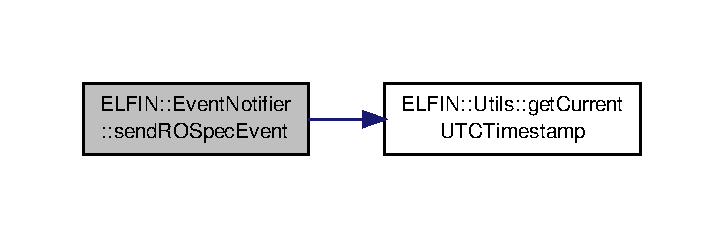
\includegraphics[width=348pt]{class_e_l_f_i_n_1_1_event_notifier_a3cf83b4e23b8c16fa587e25391dc968b_cgraph}
\end{center}
\end{figure}


\hypertarget{class_e_l_f_i_n_1_1_event_notifier_a667910f5c8ea77f2a30f989c1feaea31}{\index{E\-L\-F\-I\-N\-::\-Event\-Notifier@{E\-L\-F\-I\-N\-::\-Event\-Notifier}!send\-Spec\-Loop\-Event@{send\-Spec\-Loop\-Event}}
\index{send\-Spec\-Loop\-Event@{send\-Spec\-Loop\-Event}!ELFIN::EventNotifier@{E\-L\-F\-I\-N\-::\-Event\-Notifier}}
\subsubsection[{send\-Spec\-Loop\-Event}]{\setlength{\rightskip}{0pt plus 5cm}int E\-L\-F\-I\-N\-::\-Event\-Notifier\-::send\-Spec\-Loop\-Event (
\begin{DoxyParamCaption}
\item[{L\-L\-R\-P\-::llrp\-\_\-u32\-\_\-t}]{R\-O\-Spec\-I\-D, }
\item[{L\-L\-R\-P\-::llrp\-\_\-u32\-\_\-t}]{Loop\-Count}
\end{DoxyParamCaption}
)}}\label{class_e_l_f_i_n_1_1_event_notifier_a667910f5c8ea77f2a30f989c1feaea31}


Send corresponding event, if that event notification is enabled. 



Definition at line 105 of file Event\-Notifier.\-cpp.



Here is the call graph for this function\-:
\nopagebreak
\begin{figure}[H]
\begin{center}
\leavevmode
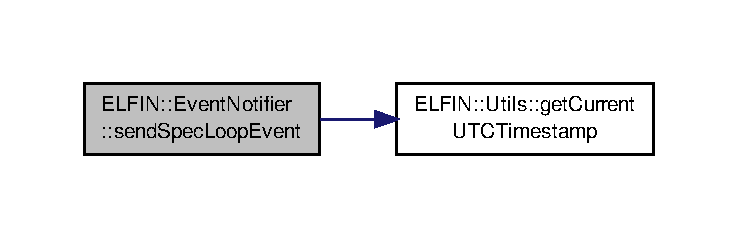
\includegraphics[width=350pt]{class_e_l_f_i_n_1_1_event_notifier_a667910f5c8ea77f2a30f989c1feaea31_cgraph}
\end{center}
\end{figure}




The documentation for this class was generated from the following files\-:\begin{DoxyCompactItemize}
\item 
elfin\-\_\-src/\hyperlink{_event_notifier_8h}{Event\-Notifier.\-h}\item 
elfin\-\_\-src/\hyperlink{_event_notifier_8cpp}{Event\-Notifier.\-cpp}\end{DoxyCompactItemize}

\hypertarget{class_e_l_f_i_n_1_1_g_p_i_event_listener}{\section{E\-L\-F\-I\-N\-:\-:G\-P\-I\-Event\-Listener Class Reference}
\label{class_e_l_f_i_n_1_1_g_p_i_event_listener}\index{E\-L\-F\-I\-N\-::\-G\-P\-I\-Event\-Listener@{E\-L\-F\-I\-N\-::\-G\-P\-I\-Event\-Listener}}
}


Interface for handling the signal from the G\-P\-I port of L\-L\-R\-P Reader.  




{\ttfamily \#include $<$G\-P\-I\-Event\-Listener.\-h$>$}



Inheritance diagram for E\-L\-F\-I\-N\-:\-:G\-P\-I\-Event\-Listener\-:
\nopagebreak
\begin{figure}[H]
\begin{center}
\leavevmode
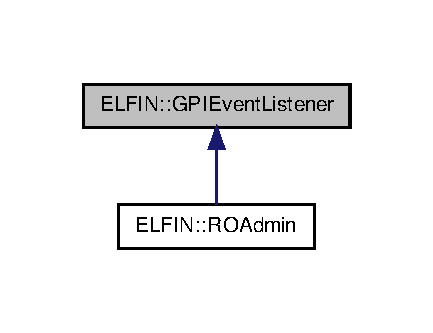
\includegraphics[width=208pt]{class_e_l_f_i_n_1_1_g_p_i_event_listener__inherit__graph}
\end{center}
\end{figure}
\subsection*{Public Member Functions}
\begin{DoxyCompactItemize}
\item 
\hyperlink{class_e_l_f_i_n_1_1_g_p_i_event_listener_a663349d73ed9d1348f970bddb342901d}{G\-P\-I\-Event\-Listener} ()
\begin{DoxyCompactList}\small\item\em Constructor of \hyperlink{class_e_l_f_i_n_1_1_g_p_i_event_listener}{G\-P\-I\-Event\-Listener} class. \end{DoxyCompactList}\item 
virtual \hyperlink{class_e_l_f_i_n_1_1_g_p_i_event_listener_a16d54d415de14ebd57211f6789ee1a3b}{$\sim$\-G\-P\-I\-Event\-Listener} ()
\begin{DoxyCompactList}\small\item\em Destructor of \hyperlink{class_e_l_f_i_n_1_1_g_p_i_event_listener}{G\-P\-I\-Event\-Listener} class. \end{DoxyCompactList}\item 
virtual void \hyperlink{class_e_l_f_i_n_1_1_g_p_i_event_listener_a5afdbda5a841643ca219f1e4bd3cad4f}{on\-G\-P\-I\-Event} (L\-L\-R\-P\-::llrp\-\_\-u16\-\_\-t G\-P\-I\-Port\-Num, enum L\-L\-R\-P\-::\-E\-G\-P\-I\-Port\-State G\-P\-I\-Event)=0
\begin{DoxyCompactList}\small\item\em Perform the operation with given port number of G\-P\-I port and its state. \end{DoxyCompactList}\item 
int \hyperlink{class_e_l_f_i_n_1_1_g_p_i_event_listener_aca1758c1f28701458725f318ac21a9de}{reg\-G\-P\-I\-Event} (int G\-P\-I\-Port\-Num, int G\-P\-I\-Event, int R\-O\-Spec\-I\-D, enum E\-G\-P\-I\-Trigger\-Type trig\-Type)
\begin{DoxyCompactList}\small\item\em Register G\-P\-I event to \-\_\-\-G\-P\-I\-Event\-Registry. \end{DoxyCompactList}\item 
int \hyperlink{class_e_l_f_i_n_1_1_g_p_i_event_listener_a00674b0da3cce658f584758d13c9201b}{unreg\-G\-P\-I\-Event} (int G\-P\-I\-Port\-Num, int G\-P\-I\-Event)
\begin{DoxyCompactList}\small\item\em Unregister G\-P\-I event from \-\_\-\-G\-P\-I\-Event\-Registry. \end{DoxyCompactList}\end{DoxyCompactItemize}
\subsection*{Public Attributes}
\begin{DoxyCompactItemize}
\item 
\hypertarget{class_e_l_f_i_n_1_1_g_p_i_event_listener_a44ae06c56f28415591b76dcabfcc6de3}{G\-P\-I\-Event\-Registry {\bfseries \-\_\-\-G\-P\-I\-Event\-Registry}}\label{class_e_l_f_i_n_1_1_g_p_i_event_listener_a44ae06c56f28415591b76dcabfcc6de3}

\item 
\hypertarget{class_e_l_f_i_n_1_1_g_p_i_event_listener_a760b47695c99113814a982dceb6ef806}{boost\-::mutex {\bfseries \-\_\-p\-G\-P\-I\-Reg\-Lock}}\label{class_e_l_f_i_n_1_1_g_p_i_event_listener_a760b47695c99113814a982dceb6ef806}

\end{DoxyCompactItemize}


\subsection{Detailed Description}
Interface for handling the signal from the G\-P\-I port of L\-L\-R\-P Reader. 

Definition at line 21 of file G\-P\-I\-Event\-Listener.\-h.



\subsection{Constructor \& Destructor Documentation}
\hypertarget{class_e_l_f_i_n_1_1_g_p_i_event_listener_a663349d73ed9d1348f970bddb342901d}{\index{E\-L\-F\-I\-N\-::\-G\-P\-I\-Event\-Listener@{E\-L\-F\-I\-N\-::\-G\-P\-I\-Event\-Listener}!G\-P\-I\-Event\-Listener@{G\-P\-I\-Event\-Listener}}
\index{G\-P\-I\-Event\-Listener@{G\-P\-I\-Event\-Listener}!ELFIN::GPIEventListener@{E\-L\-F\-I\-N\-::\-G\-P\-I\-Event\-Listener}}
\subsubsection[{G\-P\-I\-Event\-Listener}]{\setlength{\rightskip}{0pt plus 5cm}E\-L\-F\-I\-N\-::\-G\-P\-I\-Event\-Listener\-::\-G\-P\-I\-Event\-Listener (
\begin{DoxyParamCaption}
{}
\end{DoxyParamCaption}
)}}\label{class_e_l_f_i_n_1_1_g_p_i_event_listener_a663349d73ed9d1348f970bddb342901d}


Constructor of \hyperlink{class_e_l_f_i_n_1_1_g_p_i_event_listener}{G\-P\-I\-Event\-Listener} class. 



Definition at line 11 of file G\-P\-I\-Event\-Listener.\-cpp.

\hypertarget{class_e_l_f_i_n_1_1_g_p_i_event_listener_a16d54d415de14ebd57211f6789ee1a3b}{\index{E\-L\-F\-I\-N\-::\-G\-P\-I\-Event\-Listener@{E\-L\-F\-I\-N\-::\-G\-P\-I\-Event\-Listener}!$\sim$\-G\-P\-I\-Event\-Listener@{$\sim$\-G\-P\-I\-Event\-Listener}}
\index{$\sim$\-G\-P\-I\-Event\-Listener@{$\sim$\-G\-P\-I\-Event\-Listener}!ELFIN::GPIEventListener@{E\-L\-F\-I\-N\-::\-G\-P\-I\-Event\-Listener}}
\subsubsection[{$\sim$\-G\-P\-I\-Event\-Listener}]{\setlength{\rightskip}{0pt plus 5cm}E\-L\-F\-I\-N\-::\-G\-P\-I\-Event\-Listener\-::$\sim$\-G\-P\-I\-Event\-Listener (
\begin{DoxyParamCaption}
{}
\end{DoxyParamCaption}
)\hspace{0.3cm}{\ttfamily [virtual]}}}\label{class_e_l_f_i_n_1_1_g_p_i_event_listener_a16d54d415de14ebd57211f6789ee1a3b}


Destructor of \hyperlink{class_e_l_f_i_n_1_1_g_p_i_event_listener}{G\-P\-I\-Event\-Listener} class. 



Definition at line 15 of file G\-P\-I\-Event\-Listener.\-cpp.



\subsection{Member Function Documentation}
\hypertarget{class_e_l_f_i_n_1_1_g_p_i_event_listener_a5afdbda5a841643ca219f1e4bd3cad4f}{\index{E\-L\-F\-I\-N\-::\-G\-P\-I\-Event\-Listener@{E\-L\-F\-I\-N\-::\-G\-P\-I\-Event\-Listener}!on\-G\-P\-I\-Event@{on\-G\-P\-I\-Event}}
\index{on\-G\-P\-I\-Event@{on\-G\-P\-I\-Event}!ELFIN::GPIEventListener@{E\-L\-F\-I\-N\-::\-G\-P\-I\-Event\-Listener}}
\subsubsection[{on\-G\-P\-I\-Event}]{\setlength{\rightskip}{0pt plus 5cm}virtual void E\-L\-F\-I\-N\-::\-G\-P\-I\-Event\-Listener\-::on\-G\-P\-I\-Event (
\begin{DoxyParamCaption}
\item[{L\-L\-R\-P\-::llrp\-\_\-u16\-\_\-t}]{G\-P\-I\-Port\-Num, }
\item[{enum L\-L\-R\-P\-::\-E\-G\-P\-I\-Port\-State}]{G\-P\-I\-Event}
\end{DoxyParamCaption}
)\hspace{0.3cm}{\ttfamily [pure virtual]}}}\label{class_e_l_f_i_n_1_1_g_p_i_event_listener_a5afdbda5a841643ca219f1e4bd3cad4f}


Perform the operation with given port number of G\-P\-I port and its state. 



Implemented in \hyperlink{class_e_l_f_i_n_1_1_r_o_admin_a652f5d46a08d1889a4bd8b2db05a805d}{E\-L\-F\-I\-N\-::\-R\-O\-Admin}.

\hypertarget{class_e_l_f_i_n_1_1_g_p_i_event_listener_aca1758c1f28701458725f318ac21a9de}{\index{E\-L\-F\-I\-N\-::\-G\-P\-I\-Event\-Listener@{E\-L\-F\-I\-N\-::\-G\-P\-I\-Event\-Listener}!reg\-G\-P\-I\-Event@{reg\-G\-P\-I\-Event}}
\index{reg\-G\-P\-I\-Event@{reg\-G\-P\-I\-Event}!ELFIN::GPIEventListener@{E\-L\-F\-I\-N\-::\-G\-P\-I\-Event\-Listener}}
\subsubsection[{reg\-G\-P\-I\-Event}]{\setlength{\rightskip}{0pt plus 5cm}int E\-L\-F\-I\-N\-::\-G\-P\-I\-Event\-Listener\-::reg\-G\-P\-I\-Event (
\begin{DoxyParamCaption}
\item[{int}]{G\-P\-I\-Port\-Num, }
\item[{int}]{G\-P\-I\-Event, }
\item[{int}]{R\-O\-Spec\-I\-D, }
\item[{enum E\-G\-P\-I\-Trigger\-Type}]{trig\-Type}
\end{DoxyParamCaption}
)}}\label{class_e_l_f_i_n_1_1_g_p_i_event_listener_aca1758c1f28701458725f318ac21a9de}


Register G\-P\-I event to \-\_\-\-G\-P\-I\-Event\-Registry. 



Definition at line 20 of file G\-P\-I\-Event\-Listener.\-cpp.

\hypertarget{class_e_l_f_i_n_1_1_g_p_i_event_listener_a00674b0da3cce658f584758d13c9201b}{\index{E\-L\-F\-I\-N\-::\-G\-P\-I\-Event\-Listener@{E\-L\-F\-I\-N\-::\-G\-P\-I\-Event\-Listener}!unreg\-G\-P\-I\-Event@{unreg\-G\-P\-I\-Event}}
\index{unreg\-G\-P\-I\-Event@{unreg\-G\-P\-I\-Event}!ELFIN::GPIEventListener@{E\-L\-F\-I\-N\-::\-G\-P\-I\-Event\-Listener}}
\subsubsection[{unreg\-G\-P\-I\-Event}]{\setlength{\rightskip}{0pt plus 5cm}int E\-L\-F\-I\-N\-::\-G\-P\-I\-Event\-Listener\-::unreg\-G\-P\-I\-Event (
\begin{DoxyParamCaption}
\item[{int}]{G\-P\-I\-Port\-Num, }
\item[{int}]{G\-P\-I\-Event}
\end{DoxyParamCaption}
)}}\label{class_e_l_f_i_n_1_1_g_p_i_event_listener_a00674b0da3cce658f584758d13c9201b}


Unregister G\-P\-I event from \-\_\-\-G\-P\-I\-Event\-Registry. 



Definition at line 36 of file G\-P\-I\-Event\-Listener.\-cpp.



The documentation for this class was generated from the following files\-:\begin{DoxyCompactItemize}
\item 
elfin\-\_\-src/\hyperlink{_g_p_i_event_listener_8h}{G\-P\-I\-Event\-Listener.\-h}\item 
elfin\-\_\-src/\hyperlink{_g_p_i_event_listener_8cpp}{G\-P\-I\-Event\-Listener.\-cpp}\end{DoxyCompactItemize}

\hypertarget{class_e_l_f_i_n_1_1_l_l_r_p_core}{\section{E\-L\-F\-I\-N\-:\-:L\-L\-R\-P\-Core Class Reference}
\label{class_e_l_f_i_n_1_1_l_l_r_p_core}\index{E\-L\-F\-I\-N\-::\-L\-L\-R\-P\-Core@{E\-L\-F\-I\-N\-::\-L\-L\-R\-P\-Core}}
}


L\-L\-R\-P Core Operation Component.  




{\ttfamily \#include $<$L\-L\-R\-P\-Core.\-h$>$}



Collaboration diagram for E\-L\-F\-I\-N\-:\-:L\-L\-R\-P\-Core\-:
\nopagebreak
\begin{figure}[H]
\begin{center}
\leavevmode
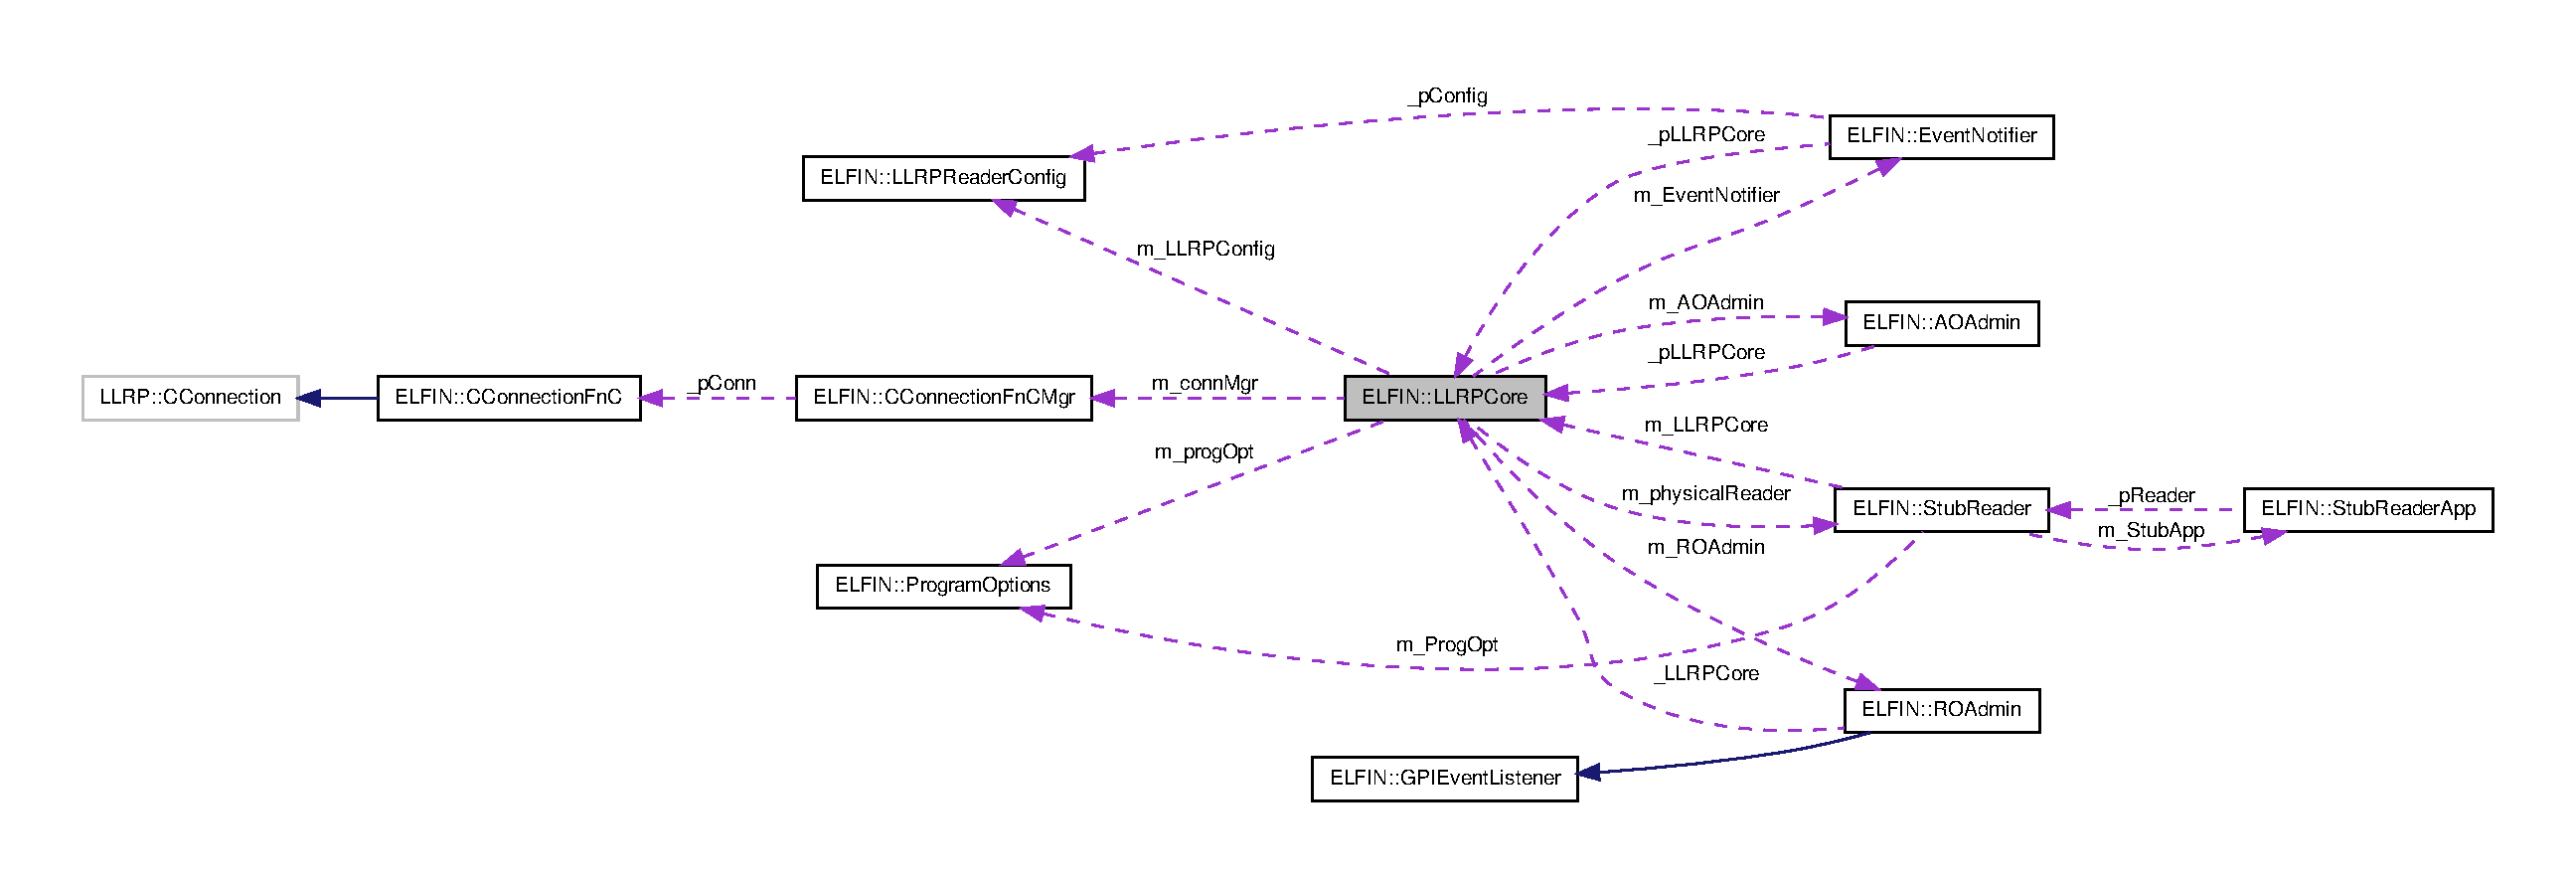
\includegraphics[width=350pt]{class_e_l_f_i_n_1_1_l_l_r_p_core__coll__graph}
\end{center}
\end{figure}
\subsection*{Public Member Functions}
\begin{DoxyCompactItemize}
\item 
\hyperlink{class_e_l_f_i_n_1_1_l_l_r_p_core_ac9ab3ee0620427813694e1c9b0ad1f80}{L\-L\-R\-P\-Core} (\hyperlink{class_e_l_f_i_n_1_1_program_options}{Program\-Options} $\ast$\-\_\-\-\_\-prog\-Opt)
\begin{DoxyCompactList}\small\item\em Constructor of \hyperlink{class_e_l_f_i_n_1_1_l_l_r_p_core}{L\-L\-R\-P\-Core} class. \end{DoxyCompactList}\item 
\hyperlink{class_e_l_f_i_n_1_1_l_l_r_p_core_ac6a776c45e59d366b39714f4d313cf30}{$\sim$\-L\-L\-R\-P\-Core} ()
\begin{DoxyCompactList}\small\item\em Destructor of \hyperlink{class_e_l_f_i_n_1_1_l_l_r_p_core}{L\-L\-R\-P\-Core} class. \end{DoxyCompactList}\item 
int \hyperlink{class_e_l_f_i_n_1_1_l_l_r_p_core_a70f26fde25b719082c2738e816e25438}{init} ()
\begin{DoxyCompactList}\small\item\em Initialize \hyperlink{class_e_l_f_i_n_1_1_l_l_r_p_core}{L\-L\-R\-P\-Core} object by setting default values and instantiating all required objects. \end{DoxyCompactList}\item 
int \hyperlink{class_e_l_f_i_n_1_1_l_l_r_p_core_aa0a970f6209038d2e89a2957c89c4570}{clear} ()
\begin{DoxyCompactList}\small\item\em Destroy all required objects and return to the initial state. \end{DoxyCompactList}\item 
int \hyperlink{class_e_l_f_i_n_1_1_l_l_r_p_core_a96cf0d4f95c33a628b4c7ea358a9c19a}{start\-Connection} ()
\begin{DoxyCompactList}\small\item\em Prepare connection to the Fn\-C server. Initiate connection or wait for connection, according to the {\itshape reader\-Initiated} option. \end{DoxyCompactList}\item 
int \hyperlink{class_e_l_f_i_n_1_1_l_l_r_p_core_a7fb97667d470bfddac25da751cf8480e}{run} ()
\begin{DoxyCompactList}\small\item\em Start L\-L\-R\-P Wrapper. Stub\-App should execute this method to run the L\-L\-R\-P Wrapper. \end{DoxyCompactList}\item 
int \hyperlink{class_e_l_f_i_n_1_1_l_l_r_p_core_ab35aa971a25103f0e288bf6cdbd198d0}{set\-Reader\-Config} (L\-L\-R\-P\-::\-C\-Message $\ast$p\-Message)
\begin{DoxyCompactList}\small\item\em Set the configuration of L\-L\-R\-P\-Reader with S\-E\-T\-\_\-\-R\-E\-A\-D\-E\-R\-\_\-\-C\-O\-N\-F\-I\-G message object. \end{DoxyCompactList}\item 
int \hyperlink{class_e_l_f_i_n_1_1_l_l_r_p_core_a606a6a467e33b1727e48a283990d0383}{load\-Default\-Config\-File} ()
\begin{DoxyCompactList}\small\item\em Load default S\-E\-T\-\_\-\-R\-E\-A\-D\-E\-R\-\_\-\-C\-O\-N\-F\-I\-G message from \hyperlink{class_e_l_f_i_n_1_1_l_l_r_p_reader_config}{L\-L\-R\-P\-Reader\-Config} object and apply it to L\-L\-R\-P Wrapper. \end{DoxyCompactList}\item 
int \hyperlink{class_e_l_f_i_n_1_1_l_l_r_p_core_a9aebe95ba139b752ad0575c483ec6f8a}{connect\-Reader\-App} (\hyperlink{class_e_l_f_i_n_1_1_stub_reader_app}{Stub\-Reader\-App} $\ast$\-\_\-\-\_\-p\-Stub\-App)
\begin{DoxyCompactList}\small\item\em Connect the Stub\-Reader\-App(or the class which inherits Stub\-Reader\-App) to \hyperlink{class_e_l_f_i_n_1_1_stub_reader}{Stub\-Reader}. \end{DoxyCompactList}\item 
int \hyperlink{class_e_l_f_i_n_1_1_l_l_r_p_core_abcc0f5f2a372cffaaf1ece1c4397576e}{send\-Message} (L\-L\-R\-P\-::\-C\-Message $\ast$\-\_\-\-\_\-p\-Message)
\begin{DoxyCompactList}\small\item\em Proxy method of \hyperlink{class_e_l_f_i_n_1_1_c_connection_fn_c_mgr_a48b283f30ddd8c2b0c2ed55e844085f8}{C\-Connection\-Fn\-C\-Mgr\-::send\-Message}. \end{DoxyCompactList}\item 
int \hyperlink{class_e_l_f_i_n_1_1_l_l_r_p_core_a37541d7698fb45e69c96c5d4b864d30a}{is\-Connected} ()
\begin{DoxyCompactList}\small\item\em Proxy method of \hyperlink{class_e_l_f_i_n_1_1_c_connection_fn_c_mgr_aa27f8bb83349b52dffe670824cfa0e53}{C\-Connection\-Fn\-C\-Mgr\-::is\-Connected}. \end{DoxyCompactList}\end{DoxyCompactItemize}
\subsection*{Static Public Member Functions}
\begin{DoxyCompactItemize}
\item 
static void \hyperlink{class_e_l_f_i_n_1_1_l_l_r_p_core_a6fe47b7e4999ced885a160f0c1094a56}{set\-Log\-Level} (enum E\-Log\-Type p\-Log\-Level)
\begin{DoxyCompactList}\small\item\em Set the log level of L\-L\-R\-P Wrapper. \end{DoxyCompactList}\end{DoxyCompactItemize}
\subsection*{Public Attributes}
\begin{DoxyCompactItemize}
\item 
\hypertarget{class_e_l_f_i_n_1_1_l_l_r_p_core_aa2ada2320d5f806217edf532ef92e229}{\hyperlink{class_e_l_f_i_n_1_1_program_options}{Program\-Options} $\ast$ {\bfseries m\-\_\-prog\-Opt}}\label{class_e_l_f_i_n_1_1_l_l_r_p_core_aa2ada2320d5f806217edf532ef92e229}

\item 
\hypertarget{class_e_l_f_i_n_1_1_l_l_r_p_core_a9c935c84e1308e257a8ccdd727a289cc}{\hyperlink{class_e_l_f_i_n_1_1_l_l_r_p_reader_config}{L\-L\-R\-P\-Reader\-Config} $\ast$ {\bfseries m\-\_\-\-L\-L\-R\-P\-Config}}\label{class_e_l_f_i_n_1_1_l_l_r_p_core_a9c935c84e1308e257a8ccdd727a289cc}

\item 
\hypertarget{class_e_l_f_i_n_1_1_l_l_r_p_core_a52de6e6859165a7713c667b582e07df2}{\hyperlink{class_e_l_f_i_n_1_1_stub_reader}{Stub\-Reader} $\ast$ {\bfseries m\-\_\-physical\-Reader}}\label{class_e_l_f_i_n_1_1_l_l_r_p_core_a52de6e6859165a7713c667b582e07df2}

\item 
\hypertarget{class_e_l_f_i_n_1_1_l_l_r_p_core_a0756fd49e8a3653ee8189aa8b4d2c89c}{\hyperlink{class_e_l_f_i_n_1_1_r_o_admin}{R\-O\-Admin} $\ast$ {\bfseries m\-\_\-\-R\-O\-Admin}}\label{class_e_l_f_i_n_1_1_l_l_r_p_core_a0756fd49e8a3653ee8189aa8b4d2c89c}

\item 
\hypertarget{class_e_l_f_i_n_1_1_l_l_r_p_core_a56439c1e6a97aeb00500b3823bad1319}{\hyperlink{class_e_l_f_i_n_1_1_a_o_admin}{A\-O\-Admin} $\ast$ {\bfseries m\-\_\-\-A\-O\-Admin}}\label{class_e_l_f_i_n_1_1_l_l_r_p_core_a56439c1e6a97aeb00500b3823bad1319}

\item 
\hypertarget{class_e_l_f_i_n_1_1_l_l_r_p_core_ace170f33e43a439da45dc30f97f544e5}{\hyperlink{class_e_l_f_i_n_1_1_c_connection_fn_c_mgr}{C\-Connection\-Fn\-C\-Mgr} $\ast$ {\bfseries m\-\_\-conn\-Mgr}}\label{class_e_l_f_i_n_1_1_l_l_r_p_core_ace170f33e43a439da45dc30f97f544e5}

\item 
\hypertarget{class_e_l_f_i_n_1_1_l_l_r_p_core_ad24f08548d029d580939391dbd90c684}{\hyperlink{class_e_l_f_i_n_1_1_event_notifier}{Event\-Notifier} $\ast$ {\bfseries m\-\_\-\-Event\-Notifier}}\label{class_e_l_f_i_n_1_1_l_l_r_p_core_ad24f08548d029d580939391dbd90c684}

\item 
\hypertarget{class_e_l_f_i_n_1_1_l_l_r_p_core_a2d2a95baf401ee9e616ddbe408904629}{boost\-::mutex {\bfseries m\-\_\-init\-Lock}}\label{class_e_l_f_i_n_1_1_l_l_r_p_core_a2d2a95baf401ee9e616ddbe408904629}

\item 
\hypertarget{class_e_l_f_i_n_1_1_l_l_r_p_core_a581f73b58235596f905942612a7c9af4}{int {\bfseries m\-\_\-shutdown}}\label{class_e_l_f_i_n_1_1_l_l_r_p_core_a581f73b58235596f905942612a7c9af4}

\item 
\hypertarget{class_e_l_f_i_n_1_1_l_l_r_p_core_a9c1e781c40fc52f15e43a1ba83845f94}{int {\bfseries m\-\_\-received\-Close\-Connection}}\label{class_e_l_f_i_n_1_1_l_l_r_p_core_a9c1e781c40fc52f15e43a1ba83845f94}

\item 
\hypertarget{class_e_l_f_i_n_1_1_l_l_r_p_core_a6cb3cd955103f01ecd6c5eb4f887287e}{int {\bfseries m\-\_\-just\-Inited}}\label{class_e_l_f_i_n_1_1_l_l_r_p_core_a6cb3cd955103f01ecd6c5eb4f887287e}

\end{DoxyCompactItemize}
\subsection*{Private Member Functions}
\begin{DoxyCompactItemize}
\item 
Result\-\_\-t \hyperlink{class_e_l_f_i_n_1_1_l_l_r_p_core_ab4c1fdb043b0ee56c29e8c3973ef609d}{get\-Error\-Result} ()
\begin{DoxyCompactList}\small\item\em Create Result\-\_\-t based on the m\-\_\-\-Error\-Details. \end{DoxyCompactList}\end{DoxyCompactItemize}
{\bf }\par
\begin{DoxyCompactItemize}
\item 
int \hyperlink{class_e_l_f_i_n_1_1_l_l_r_p_core_a68fc07b9a02e9d81abaf3536d3be2bb3}{handle\-Get\-Supported\-Version} (L\-L\-R\-P\-::\-C\-Message $\ast$\-\_\-p\-Cmd, L\-L\-R\-P\-::\-C\-Message $\ast$$\ast$\-\_\-p\-Rsp)
\begin{DoxyCompactList}\small\item\em L\-L\-R\-P message handler method. \end{DoxyCompactList}\item 
int \hyperlink{class_e_l_f_i_n_1_1_l_l_r_p_core_a1e32c1a8d11bcf11f5d8143eac90fd91}{handle\-Set\-Protocol\-Version} (L\-L\-R\-P\-::\-C\-Message $\ast$\-\_\-p\-Cmd, L\-L\-R\-P\-::\-C\-Message $\ast$$\ast$\-\_\-p\-Rsp)
\item 
int \hyperlink{class_e_l_f_i_n_1_1_l_l_r_p_core_a6513619f9917762db82e6b145edada6d}{handle\-Get\-Reader\-Capabilities} (L\-L\-R\-P\-::\-C\-Message $\ast$\-\_\-p\-Cmd, L\-L\-R\-P\-::\-C\-Message $\ast$$\ast$\-\_\-p\-Rsp)
\begin{DoxyCompactList}\small\item\em L\-L\-R\-P message handler method. \end{DoxyCompactList}\item 
int \hyperlink{class_e_l_f_i_n_1_1_l_l_r_p_core_ada340ab8828c0e5cbe3252b63e23282c}{handle\-Add\-R\-O\-Spec} (L\-L\-R\-P\-::\-C\-Message $\ast$\-\_\-p\-Cmd, L\-L\-R\-P\-::\-C\-Message $\ast$$\ast$\-\_\-p\-Rsp)
\begin{DoxyCompactList}\small\item\em L\-L\-R\-P message handler method. \end{DoxyCompactList}\item 
int \hyperlink{class_e_l_f_i_n_1_1_l_l_r_p_core_a4512038068328877714c3c596e7785af}{handle\-Delete\-R\-O\-Spec} (L\-L\-R\-P\-::\-C\-Message $\ast$\-\_\-p\-Cmd, L\-L\-R\-P\-::\-C\-Message $\ast$$\ast$\-\_\-p\-Rsp)
\begin{DoxyCompactList}\small\item\em L\-L\-R\-P message handler method. \end{DoxyCompactList}\item 
int \hyperlink{class_e_l_f_i_n_1_1_l_l_r_p_core_a4b146a62a2a78e1c73862cd3d047c947}{handle\-Start\-R\-O\-Spec} (L\-L\-R\-P\-::\-C\-Message $\ast$\-\_\-p\-Cmd, L\-L\-R\-P\-::\-C\-Message $\ast$$\ast$\-\_\-p\-Rsp)
\begin{DoxyCompactList}\small\item\em L\-L\-R\-P message handler method. \end{DoxyCompactList}\item 
int \hyperlink{class_e_l_f_i_n_1_1_l_l_r_p_core_a3de21a966ba229befbbbf0408fe4fc8e}{handle\-Stop\-R\-O\-Spec} (L\-L\-R\-P\-::\-C\-Message $\ast$\-\_\-p\-Cmd, L\-L\-R\-P\-::\-C\-Message $\ast$$\ast$\-\_\-p\-Rsp)
\begin{DoxyCompactList}\small\item\em L\-L\-R\-P message handler method. \end{DoxyCompactList}\item 
int \hyperlink{class_e_l_f_i_n_1_1_l_l_r_p_core_ade8bc074fb35e9c20d05dfa022bfeac2}{handle\-Enable\-R\-O\-Spec} (L\-L\-R\-P\-::\-C\-Message $\ast$\-\_\-p\-Cmd, L\-L\-R\-P\-::\-C\-Message $\ast$$\ast$\-\_\-p\-Rsp)
\begin{DoxyCompactList}\small\item\em L\-L\-R\-P message handler method. \end{DoxyCompactList}\item 
int \hyperlink{class_e_l_f_i_n_1_1_l_l_r_p_core_a1e65a470f564ab1e33db0aed0845ec79}{handle\-Disable\-R\-O\-Spec} (L\-L\-R\-P\-::\-C\-Message $\ast$\-\_\-p\-Cmd, L\-L\-R\-P\-::\-C\-Message $\ast$$\ast$\-\_\-p\-Rsp)
\begin{DoxyCompactList}\small\item\em L\-L\-R\-P message handler method. \end{DoxyCompactList}\item 
int \hyperlink{class_e_l_f_i_n_1_1_l_l_r_p_core_add0b12e57fcac6dd50a862a48a4bf31e}{handle\-Get\-R\-O\-Specs} (L\-L\-R\-P\-::\-C\-Message $\ast$\-\_\-p\-Cmd, L\-L\-R\-P\-::\-C\-Message $\ast$$\ast$\-\_\-p\-Rsp)
\begin{DoxyCompactList}\small\item\em L\-L\-R\-P message handler method. \end{DoxyCompactList}\item 
int \hyperlink{class_e_l_f_i_n_1_1_l_l_r_p_core_a17bbb63e25368171f95c5f20055f7bc9}{handle\-Add\-Access\-Spec} (L\-L\-R\-P\-::\-C\-Message $\ast$\-\_\-p\-Cmd, L\-L\-R\-P\-::\-C\-Message $\ast$$\ast$\-\_\-p\-Rsp)
\begin{DoxyCompactList}\small\item\em L\-L\-R\-P message handler method. \end{DoxyCompactList}\item 
int \hyperlink{class_e_l_f_i_n_1_1_l_l_r_p_core_a04e40f0768473c1f30a475c8fd30134d}{handle\-Delete\-Access\-Spec} (L\-L\-R\-P\-::\-C\-Message $\ast$\-\_\-p\-Cmd, L\-L\-R\-P\-::\-C\-Message $\ast$$\ast$\-\_\-p\-Rsp)
\begin{DoxyCompactList}\small\item\em L\-L\-R\-P message handler method. \end{DoxyCompactList}\item 
int \hyperlink{class_e_l_f_i_n_1_1_l_l_r_p_core_aede685c6e02f5a531d554a98f03a040e}{handle\-Enable\-Access\-Spec} (L\-L\-R\-P\-::\-C\-Message $\ast$\-\_\-p\-Cmd, L\-L\-R\-P\-::\-C\-Message $\ast$$\ast$\-\_\-p\-Rsp)
\begin{DoxyCompactList}\small\item\em L\-L\-R\-P message handler method. \end{DoxyCompactList}\item 
int \hyperlink{class_e_l_f_i_n_1_1_l_l_r_p_core_ad3cb7e5ea78aebac7519ec7f49107f43}{handle\-Disable\-Access\-Spec} (L\-L\-R\-P\-::\-C\-Message $\ast$\-\_\-p\-Cmd, L\-L\-R\-P\-::\-C\-Message $\ast$$\ast$\-\_\-p\-Rsp)
\begin{DoxyCompactList}\small\item\em L\-L\-R\-P message handler method. \end{DoxyCompactList}\item 
int \hyperlink{class_e_l_f_i_n_1_1_l_l_r_p_core_a0fe9819cb4d6f4f2fe7db92bb9d4c6f7}{handle\-Get\-Access\-Specs} (L\-L\-R\-P\-::\-C\-Message $\ast$\-\_\-p\-Cmd, L\-L\-R\-P\-::\-C\-Message $\ast$$\ast$\-\_\-p\-Rsp)
\begin{DoxyCompactList}\small\item\em L\-L\-R\-P message handler method. \end{DoxyCompactList}\item 
int \hyperlink{class_e_l_f_i_n_1_1_l_l_r_p_core_a875e8917fc9f44232d1355f3d91a76e2}{handle\-Get\-Reader\-Config} (L\-L\-R\-P\-::\-C\-Message $\ast$\-\_\-p\-Cmd, L\-L\-R\-P\-::\-C\-Message $\ast$$\ast$\-\_\-p\-Rsp)
\begin{DoxyCompactList}\small\item\em L\-L\-R\-P message handler method. \end{DoxyCompactList}\item 
int \hyperlink{class_e_l_f_i_n_1_1_l_l_r_p_core_a0065a7307c4ea46db3fea2cd109bc1e1}{handle\-Set\-Reader\-Config} (L\-L\-R\-P\-::\-C\-Message $\ast$\-\_\-p\-Cmd, L\-L\-R\-P\-::\-C\-Message $\ast$$\ast$\-\_\-p\-Rsp)
\item 
int \hyperlink{class_e_l_f_i_n_1_1_l_l_r_p_core_a7fd1997d7f4e08d037ea9a9f666b4371}{handle\-Close\-Connection} (L\-L\-R\-P\-::\-C\-Message $\ast$\-\_\-p\-Cmd, L\-L\-R\-P\-::\-C\-Message $\ast$$\ast$\-\_\-p\-Rsp)
\begin{DoxyCompactList}\small\item\em L\-L\-R\-P message handler method. \end{DoxyCompactList}\end{DoxyCompactItemize}

\subsection*{Private Attributes}
\begin{DoxyCompactItemize}
\item 
\hypertarget{class_e_l_f_i_n_1_1_l_l_r_p_core_a872a1dbe07c09d91937f3329c6bb0b8a}{L\-L\-R\-P\-::\-C\-Error\-Details {\bfseries m\-\_\-\-Error\-Details}}\label{class_e_l_f_i_n_1_1_l_l_r_p_core_a872a1dbe07c09d91937f3329c6bb0b8a}

\end{DoxyCompactItemize}


\subsection{Detailed Description}
L\-L\-R\-P Core Operation Component. 

Definition at line 30 of file L\-L\-R\-P\-Core.\-h.



\subsection{Constructor \& Destructor Documentation}
\hypertarget{class_e_l_f_i_n_1_1_l_l_r_p_core_ac9ab3ee0620427813694e1c9b0ad1f80}{\index{E\-L\-F\-I\-N\-::\-L\-L\-R\-P\-Core@{E\-L\-F\-I\-N\-::\-L\-L\-R\-P\-Core}!L\-L\-R\-P\-Core@{L\-L\-R\-P\-Core}}
\index{L\-L\-R\-P\-Core@{L\-L\-R\-P\-Core}!ELFIN::LLRPCore@{E\-L\-F\-I\-N\-::\-L\-L\-R\-P\-Core}}
\subsubsection[{L\-L\-R\-P\-Core}]{\setlength{\rightskip}{0pt plus 5cm}E\-L\-F\-I\-N\-::\-L\-L\-R\-P\-Core\-::\-L\-L\-R\-P\-Core (
\begin{DoxyParamCaption}
\item[{{\bf Program\-Options} $\ast$}]{\-\_\-\-\_\-prog\-Opt}
\end{DoxyParamCaption}
)}}\label{class_e_l_f_i_n_1_1_l_l_r_p_core_ac9ab3ee0620427813694e1c9b0ad1f80}


Constructor of \hyperlink{class_e_l_f_i_n_1_1_l_l_r_p_core}{L\-L\-R\-P\-Core} class. 



Definition at line 19 of file L\-L\-R\-P\-Core.\-cpp.



Here is the call graph for this function\-:
\nopagebreak
\begin{figure}[H]
\begin{center}
\leavevmode
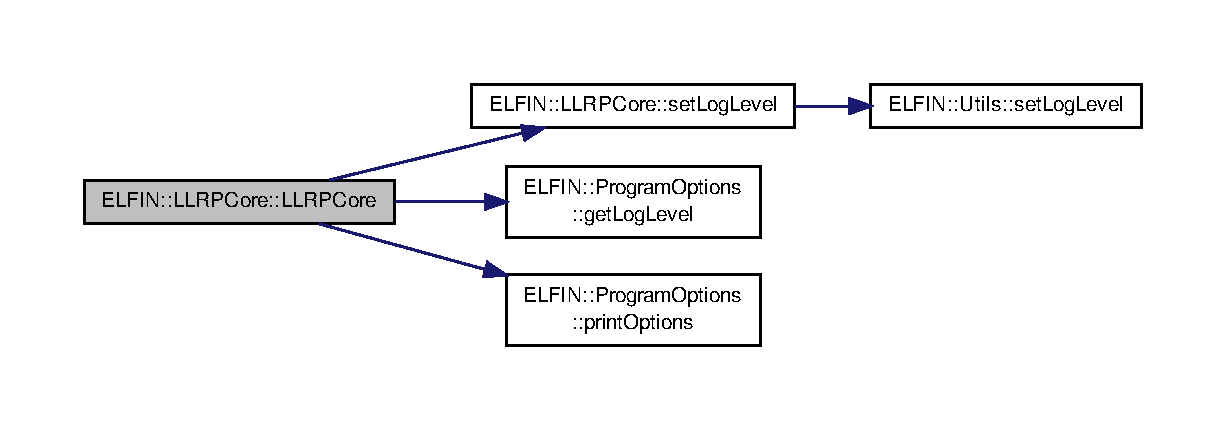
\includegraphics[width=350pt]{class_e_l_f_i_n_1_1_l_l_r_p_core_ac9ab3ee0620427813694e1c9b0ad1f80_cgraph}
\end{center}
\end{figure}


\hypertarget{class_e_l_f_i_n_1_1_l_l_r_p_core_ac6a776c45e59d366b39714f4d313cf30}{\index{E\-L\-F\-I\-N\-::\-L\-L\-R\-P\-Core@{E\-L\-F\-I\-N\-::\-L\-L\-R\-P\-Core}!$\sim$\-L\-L\-R\-P\-Core@{$\sim$\-L\-L\-R\-P\-Core}}
\index{$\sim$\-L\-L\-R\-P\-Core@{$\sim$\-L\-L\-R\-P\-Core}!ELFIN::LLRPCore@{E\-L\-F\-I\-N\-::\-L\-L\-R\-P\-Core}}
\subsubsection[{$\sim$\-L\-L\-R\-P\-Core}]{\setlength{\rightskip}{0pt plus 5cm}E\-L\-F\-I\-N\-::\-L\-L\-R\-P\-Core\-::$\sim$\-L\-L\-R\-P\-Core (
\begin{DoxyParamCaption}
{}
\end{DoxyParamCaption}
)}}\label{class_e_l_f_i_n_1_1_l_l_r_p_core_ac6a776c45e59d366b39714f4d313cf30}


Destructor of \hyperlink{class_e_l_f_i_n_1_1_l_l_r_p_core}{L\-L\-R\-P\-Core} class. 



Definition at line 89 of file L\-L\-R\-P\-Core.\-cpp.



\subsection{Member Function Documentation}
\hypertarget{class_e_l_f_i_n_1_1_l_l_r_p_core_aa0a970f6209038d2e89a2957c89c4570}{\index{E\-L\-F\-I\-N\-::\-L\-L\-R\-P\-Core@{E\-L\-F\-I\-N\-::\-L\-L\-R\-P\-Core}!clear@{clear}}
\index{clear@{clear}!ELFIN::LLRPCore@{E\-L\-F\-I\-N\-::\-L\-L\-R\-P\-Core}}
\subsubsection[{clear}]{\setlength{\rightskip}{0pt plus 5cm}int E\-L\-F\-I\-N\-::\-L\-L\-R\-P\-Core\-::clear (
\begin{DoxyParamCaption}
{}
\end{DoxyParamCaption}
)}}\label{class_e_l_f_i_n_1_1_l_l_r_p_core_aa0a970f6209038d2e89a2957c89c4570}


Destroy all required objects and return to the initial state. 



Definition at line 60 of file L\-L\-R\-P\-Core.\-cpp.

\hypertarget{class_e_l_f_i_n_1_1_l_l_r_p_core_a9aebe95ba139b752ad0575c483ec6f8a}{\index{E\-L\-F\-I\-N\-::\-L\-L\-R\-P\-Core@{E\-L\-F\-I\-N\-::\-L\-L\-R\-P\-Core}!connect\-Reader\-App@{connect\-Reader\-App}}
\index{connect\-Reader\-App@{connect\-Reader\-App}!ELFIN::LLRPCore@{E\-L\-F\-I\-N\-::\-L\-L\-R\-P\-Core}}
\subsubsection[{connect\-Reader\-App}]{\setlength{\rightskip}{0pt plus 5cm}int E\-L\-F\-I\-N\-::\-L\-L\-R\-P\-Core\-::connect\-Reader\-App (
\begin{DoxyParamCaption}
\item[{{\bf Stub\-Reader\-App} $\ast$}]{\-\_\-\-\_\-p\-Stub\-App}
\end{DoxyParamCaption}
)}}\label{class_e_l_f_i_n_1_1_l_l_r_p_core_a9aebe95ba139b752ad0575c483ec6f8a}


Connect the Stub\-Reader\-App(or the class which inherits Stub\-Reader\-App) to \hyperlink{class_e_l_f_i_n_1_1_stub_reader}{Stub\-Reader}. 



Definition at line 1208 of file L\-L\-R\-P\-Core.\-cpp.

\hypertarget{class_e_l_f_i_n_1_1_l_l_r_p_core_ab4c1fdb043b0ee56c29e8c3973ef609d}{\index{E\-L\-F\-I\-N\-::\-L\-L\-R\-P\-Core@{E\-L\-F\-I\-N\-::\-L\-L\-R\-P\-Core}!get\-Error\-Result@{get\-Error\-Result}}
\index{get\-Error\-Result@{get\-Error\-Result}!ELFIN::LLRPCore@{E\-L\-F\-I\-N\-::\-L\-L\-R\-P\-Core}}
\subsubsection[{get\-Error\-Result}]{\setlength{\rightskip}{0pt plus 5cm}E\-L\-F\-I\-N\-::\-Result\-\_\-t E\-L\-F\-I\-N\-::\-L\-L\-R\-P\-Core\-::get\-Error\-Result (
\begin{DoxyParamCaption}
{}
\end{DoxyParamCaption}
)\hspace{0.3cm}{\ttfamily [private]}}}\label{class_e_l_f_i_n_1_1_l_l_r_p_core_ab4c1fdb043b0ee56c29e8c3973ef609d}


Create Result\-\_\-t based on the m\-\_\-\-Error\-Details. 



Definition at line 1246 of file L\-L\-R\-P\-Core.\-cpp.



Here is the call graph for this function\-:
\nopagebreak
\begin{figure}[H]
\begin{center}
\leavevmode
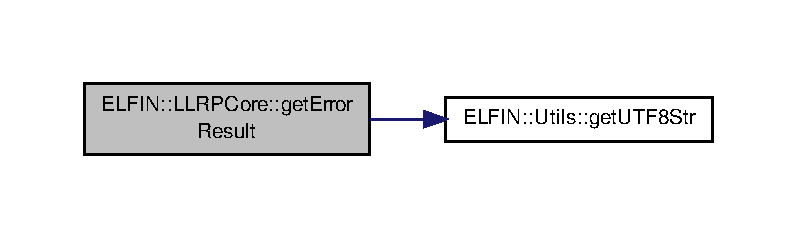
\includegraphics[width=350pt]{class_e_l_f_i_n_1_1_l_l_r_p_core_ab4c1fdb043b0ee56c29e8c3973ef609d_cgraph}
\end{center}
\end{figure}


\hypertarget{class_e_l_f_i_n_1_1_l_l_r_p_core_a17bbb63e25368171f95c5f20055f7bc9}{\index{E\-L\-F\-I\-N\-::\-L\-L\-R\-P\-Core@{E\-L\-F\-I\-N\-::\-L\-L\-R\-P\-Core}!handle\-Add\-Access\-Spec@{handle\-Add\-Access\-Spec}}
\index{handle\-Add\-Access\-Spec@{handle\-Add\-Access\-Spec}!ELFIN::LLRPCore@{E\-L\-F\-I\-N\-::\-L\-L\-R\-P\-Core}}
\subsubsection[{handle\-Add\-Access\-Spec}]{\setlength{\rightskip}{0pt plus 5cm}int E\-L\-F\-I\-N\-::\-L\-L\-R\-P\-Core\-::handle\-Add\-Access\-Spec (
\begin{DoxyParamCaption}
\item[{L\-L\-R\-P\-::\-C\-Message $\ast$}]{\-\_\-p\-Cmd, }
\item[{L\-L\-R\-P\-::\-C\-Message $\ast$$\ast$}]{\-\_\-p\-Rsp}
\end{DoxyParamCaption}
)\hspace{0.3cm}{\ttfamily [private]}}}\label{class_e_l_f_i_n_1_1_l_l_r_p_core_a17bbb63e25368171f95c5f20055f7bc9}


L\-L\-R\-P message handler method. 



Definition at line 632 of file L\-L\-R\-P\-Core.\-cpp.



Here is the call graph for this function\-:
\nopagebreak
\begin{figure}[H]
\begin{center}
\leavevmode
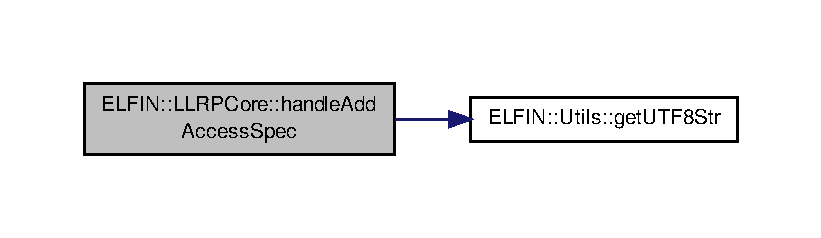
\includegraphics[width=350pt]{class_e_l_f_i_n_1_1_l_l_r_p_core_a17bbb63e25368171f95c5f20055f7bc9_cgraph}
\end{center}
\end{figure}


\hypertarget{class_e_l_f_i_n_1_1_l_l_r_p_core_ada340ab8828c0e5cbe3252b63e23282c}{\index{E\-L\-F\-I\-N\-::\-L\-L\-R\-P\-Core@{E\-L\-F\-I\-N\-::\-L\-L\-R\-P\-Core}!handle\-Add\-R\-O\-Spec@{handle\-Add\-R\-O\-Spec}}
\index{handle\-Add\-R\-O\-Spec@{handle\-Add\-R\-O\-Spec}!ELFIN::LLRPCore@{E\-L\-F\-I\-N\-::\-L\-L\-R\-P\-Core}}
\subsubsection[{handle\-Add\-R\-O\-Spec}]{\setlength{\rightskip}{0pt plus 5cm}int E\-L\-F\-I\-N\-::\-L\-L\-R\-P\-Core\-::handle\-Add\-R\-O\-Spec (
\begin{DoxyParamCaption}
\item[{L\-L\-R\-P\-::\-C\-Message $\ast$}]{\-\_\-p\-Cmd, }
\item[{L\-L\-R\-P\-::\-C\-Message $\ast$$\ast$}]{\-\_\-p\-Rsp}
\end{DoxyParamCaption}
)\hspace{0.3cm}{\ttfamily [private]}}}\label{class_e_l_f_i_n_1_1_l_l_r_p_core_ada340ab8828c0e5cbe3252b63e23282c}


L\-L\-R\-P message handler method. 



Definition at line 444 of file L\-L\-R\-P\-Core.\-cpp.



Here is the call graph for this function\-:
\nopagebreak
\begin{figure}[H]
\begin{center}
\leavevmode
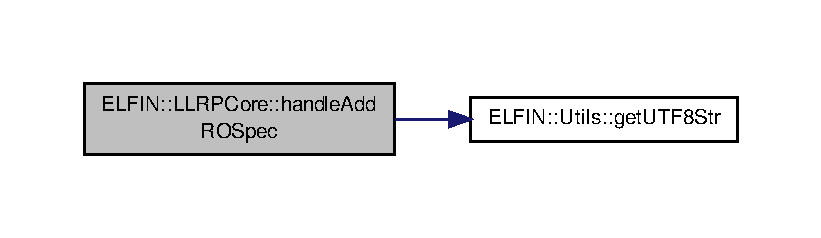
\includegraphics[width=350pt]{class_e_l_f_i_n_1_1_l_l_r_p_core_ada340ab8828c0e5cbe3252b63e23282c_cgraph}
\end{center}
\end{figure}


\hypertarget{class_e_l_f_i_n_1_1_l_l_r_p_core_a7fd1997d7f4e08d037ea9a9f666b4371}{\index{E\-L\-F\-I\-N\-::\-L\-L\-R\-P\-Core@{E\-L\-F\-I\-N\-::\-L\-L\-R\-P\-Core}!handle\-Close\-Connection@{handle\-Close\-Connection}}
\index{handle\-Close\-Connection@{handle\-Close\-Connection}!ELFIN::LLRPCore@{E\-L\-F\-I\-N\-::\-L\-L\-R\-P\-Core}}
\subsubsection[{handle\-Close\-Connection}]{\setlength{\rightskip}{0pt plus 5cm}int E\-L\-F\-I\-N\-::\-L\-L\-R\-P\-Core\-::handle\-Close\-Connection (
\begin{DoxyParamCaption}
\item[{L\-L\-R\-P\-::\-C\-Message $\ast$}]{\-\_\-p\-Cmd, }
\item[{L\-L\-R\-P\-::\-C\-Message $\ast$$\ast$}]{\-\_\-p\-Rsp}
\end{DoxyParamCaption}
)\hspace{0.3cm}{\ttfamily [private]}}}\label{class_e_l_f_i_n_1_1_l_l_r_p_core_a7fd1997d7f4e08d037ea9a9f666b4371}


L\-L\-R\-P message handler method. 



Definition at line 1151 of file L\-L\-R\-P\-Core.\-cpp.



Here is the call graph for this function\-:
\nopagebreak
\begin{figure}[H]
\begin{center}
\leavevmode
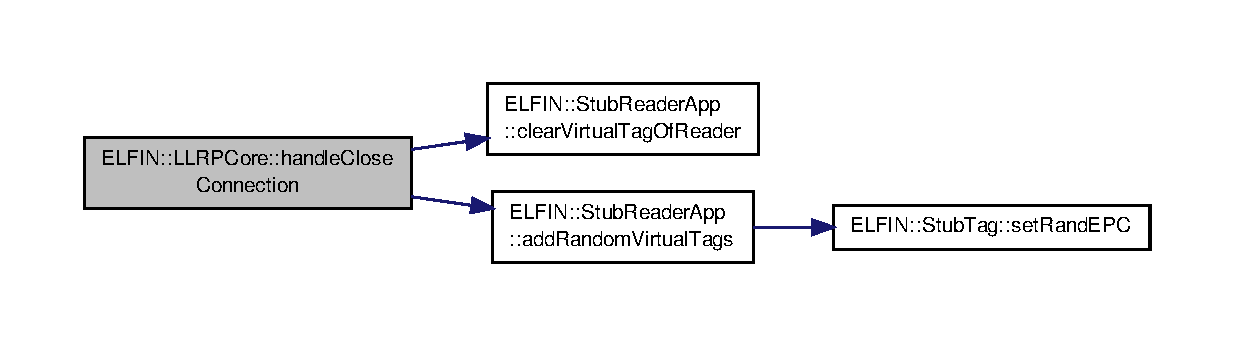
\includegraphics[width=350pt]{class_e_l_f_i_n_1_1_l_l_r_p_core_a7fd1997d7f4e08d037ea9a9f666b4371_cgraph}
\end{center}
\end{figure}


\hypertarget{class_e_l_f_i_n_1_1_l_l_r_p_core_a04e40f0768473c1f30a475c8fd30134d}{\index{E\-L\-F\-I\-N\-::\-L\-L\-R\-P\-Core@{E\-L\-F\-I\-N\-::\-L\-L\-R\-P\-Core}!handle\-Delete\-Access\-Spec@{handle\-Delete\-Access\-Spec}}
\index{handle\-Delete\-Access\-Spec@{handle\-Delete\-Access\-Spec}!ELFIN::LLRPCore@{E\-L\-F\-I\-N\-::\-L\-L\-R\-P\-Core}}
\subsubsection[{handle\-Delete\-Access\-Spec}]{\setlength{\rightskip}{0pt plus 5cm}int E\-L\-F\-I\-N\-::\-L\-L\-R\-P\-Core\-::handle\-Delete\-Access\-Spec (
\begin{DoxyParamCaption}
\item[{L\-L\-R\-P\-::\-C\-Message $\ast$}]{\-\_\-p\-Cmd, }
\item[{L\-L\-R\-P\-::\-C\-Message $\ast$$\ast$}]{\-\_\-p\-Rsp}
\end{DoxyParamCaption}
)\hspace{0.3cm}{\ttfamily [private]}}}\label{class_e_l_f_i_n_1_1_l_l_r_p_core_a04e40f0768473c1f30a475c8fd30134d}


L\-L\-R\-P message handler method. 



Definition at line 661 of file L\-L\-R\-P\-Core.\-cpp.



Here is the call graph for this function\-:
\nopagebreak
\begin{figure}[H]
\begin{center}
\leavevmode
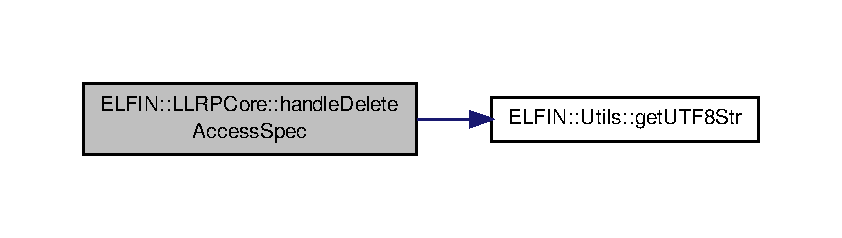
\includegraphics[width=350pt]{class_e_l_f_i_n_1_1_l_l_r_p_core_a04e40f0768473c1f30a475c8fd30134d_cgraph}
\end{center}
\end{figure}


\hypertarget{class_e_l_f_i_n_1_1_l_l_r_p_core_a4512038068328877714c3c596e7785af}{\index{E\-L\-F\-I\-N\-::\-L\-L\-R\-P\-Core@{E\-L\-F\-I\-N\-::\-L\-L\-R\-P\-Core}!handle\-Delete\-R\-O\-Spec@{handle\-Delete\-R\-O\-Spec}}
\index{handle\-Delete\-R\-O\-Spec@{handle\-Delete\-R\-O\-Spec}!ELFIN::LLRPCore@{E\-L\-F\-I\-N\-::\-L\-L\-R\-P\-Core}}
\subsubsection[{handle\-Delete\-R\-O\-Spec}]{\setlength{\rightskip}{0pt plus 5cm}int E\-L\-F\-I\-N\-::\-L\-L\-R\-P\-Core\-::handle\-Delete\-R\-O\-Spec (
\begin{DoxyParamCaption}
\item[{L\-L\-R\-P\-::\-C\-Message $\ast$}]{\-\_\-p\-Cmd, }
\item[{L\-L\-R\-P\-::\-C\-Message $\ast$$\ast$}]{\-\_\-p\-Rsp}
\end{DoxyParamCaption}
)\hspace{0.3cm}{\ttfamily [private]}}}\label{class_e_l_f_i_n_1_1_l_l_r_p_core_a4512038068328877714c3c596e7785af}


L\-L\-R\-P message handler method. 



Definition at line 472 of file L\-L\-R\-P\-Core.\-cpp.



Here is the call graph for this function\-:
\nopagebreak
\begin{figure}[H]
\begin{center}
\leavevmode
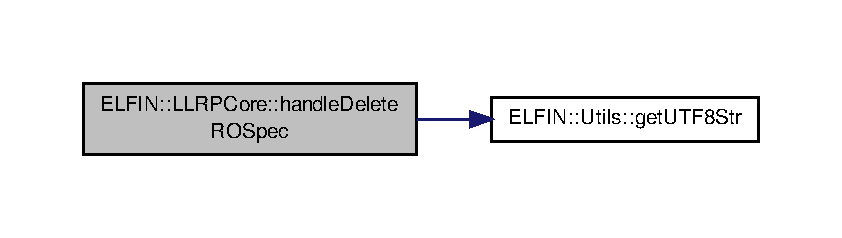
\includegraphics[width=350pt]{class_e_l_f_i_n_1_1_l_l_r_p_core_a4512038068328877714c3c596e7785af_cgraph}
\end{center}
\end{figure}


\hypertarget{class_e_l_f_i_n_1_1_l_l_r_p_core_ad3cb7e5ea78aebac7519ec7f49107f43}{\index{E\-L\-F\-I\-N\-::\-L\-L\-R\-P\-Core@{E\-L\-F\-I\-N\-::\-L\-L\-R\-P\-Core}!handle\-Disable\-Access\-Spec@{handle\-Disable\-Access\-Spec}}
\index{handle\-Disable\-Access\-Spec@{handle\-Disable\-Access\-Spec}!ELFIN::LLRPCore@{E\-L\-F\-I\-N\-::\-L\-L\-R\-P\-Core}}
\subsubsection[{handle\-Disable\-Access\-Spec}]{\setlength{\rightskip}{0pt plus 5cm}int E\-L\-F\-I\-N\-::\-L\-L\-R\-P\-Core\-::handle\-Disable\-Access\-Spec (
\begin{DoxyParamCaption}
\item[{L\-L\-R\-P\-::\-C\-Message $\ast$}]{\-\_\-p\-Cmd, }
\item[{L\-L\-R\-P\-::\-C\-Message $\ast$$\ast$}]{\-\_\-p\-Rsp}
\end{DoxyParamCaption}
)\hspace{0.3cm}{\ttfamily [private]}}}\label{class_e_l_f_i_n_1_1_l_l_r_p_core_ad3cb7e5ea78aebac7519ec7f49107f43}


L\-L\-R\-P message handler method. 



Definition at line 715 of file L\-L\-R\-P\-Core.\-cpp.



Here is the call graph for this function\-:
\nopagebreak
\begin{figure}[H]
\begin{center}
\leavevmode
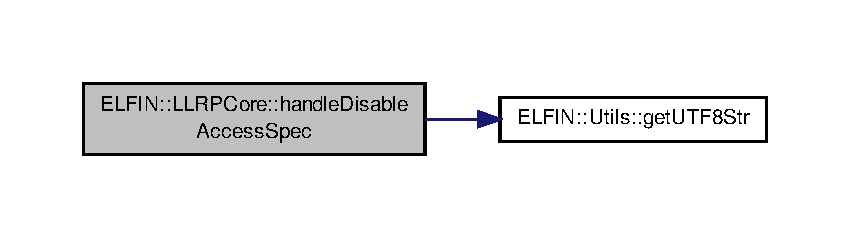
\includegraphics[width=350pt]{class_e_l_f_i_n_1_1_l_l_r_p_core_ad3cb7e5ea78aebac7519ec7f49107f43_cgraph}
\end{center}
\end{figure}


\hypertarget{class_e_l_f_i_n_1_1_l_l_r_p_core_a1e65a470f564ab1e33db0aed0845ec79}{\index{E\-L\-F\-I\-N\-::\-L\-L\-R\-P\-Core@{E\-L\-F\-I\-N\-::\-L\-L\-R\-P\-Core}!handle\-Disable\-R\-O\-Spec@{handle\-Disable\-R\-O\-Spec}}
\index{handle\-Disable\-R\-O\-Spec@{handle\-Disable\-R\-O\-Spec}!ELFIN::LLRPCore@{E\-L\-F\-I\-N\-::\-L\-L\-R\-P\-Core}}
\subsubsection[{handle\-Disable\-R\-O\-Spec}]{\setlength{\rightskip}{0pt plus 5cm}int E\-L\-F\-I\-N\-::\-L\-L\-R\-P\-Core\-::handle\-Disable\-R\-O\-Spec (
\begin{DoxyParamCaption}
\item[{L\-L\-R\-P\-::\-C\-Message $\ast$}]{\-\_\-p\-Cmd, }
\item[{L\-L\-R\-P\-::\-C\-Message $\ast$$\ast$}]{\-\_\-p\-Rsp}
\end{DoxyParamCaption}
)\hspace{0.3cm}{\ttfamily [private]}}}\label{class_e_l_f_i_n_1_1_l_l_r_p_core_a1e65a470f564ab1e33db0aed0845ec79}


L\-L\-R\-P message handler method. 



Definition at line 575 of file L\-L\-R\-P\-Core.\-cpp.



Here is the call graph for this function\-:
\nopagebreak
\begin{figure}[H]
\begin{center}
\leavevmode
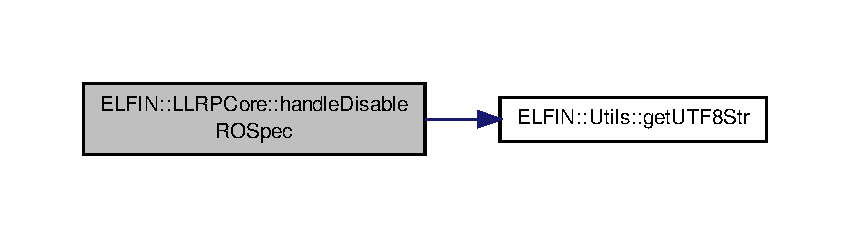
\includegraphics[width=350pt]{class_e_l_f_i_n_1_1_l_l_r_p_core_a1e65a470f564ab1e33db0aed0845ec79_cgraph}
\end{center}
\end{figure}


\hypertarget{class_e_l_f_i_n_1_1_l_l_r_p_core_aede685c6e02f5a531d554a98f03a040e}{\index{E\-L\-F\-I\-N\-::\-L\-L\-R\-P\-Core@{E\-L\-F\-I\-N\-::\-L\-L\-R\-P\-Core}!handle\-Enable\-Access\-Spec@{handle\-Enable\-Access\-Spec}}
\index{handle\-Enable\-Access\-Spec@{handle\-Enable\-Access\-Spec}!ELFIN::LLRPCore@{E\-L\-F\-I\-N\-::\-L\-L\-R\-P\-Core}}
\subsubsection[{handle\-Enable\-Access\-Spec}]{\setlength{\rightskip}{0pt plus 5cm}int E\-L\-F\-I\-N\-::\-L\-L\-R\-P\-Core\-::handle\-Enable\-Access\-Spec (
\begin{DoxyParamCaption}
\item[{L\-L\-R\-P\-::\-C\-Message $\ast$}]{\-\_\-p\-Cmd, }
\item[{L\-L\-R\-P\-::\-C\-Message $\ast$$\ast$}]{\-\_\-p\-Rsp}
\end{DoxyParamCaption}
)\hspace{0.3cm}{\ttfamily [private]}}}\label{class_e_l_f_i_n_1_1_l_l_r_p_core_aede685c6e02f5a531d554a98f03a040e}


L\-L\-R\-P message handler method. 



Definition at line 688 of file L\-L\-R\-P\-Core.\-cpp.



Here is the call graph for this function\-:
\nopagebreak
\begin{figure}[H]
\begin{center}
\leavevmode
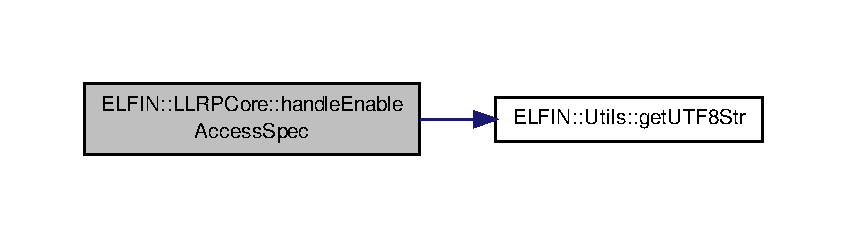
\includegraphics[width=350pt]{class_e_l_f_i_n_1_1_l_l_r_p_core_aede685c6e02f5a531d554a98f03a040e_cgraph}
\end{center}
\end{figure}


\hypertarget{class_e_l_f_i_n_1_1_l_l_r_p_core_ade8bc074fb35e9c20d05dfa022bfeac2}{\index{E\-L\-F\-I\-N\-::\-L\-L\-R\-P\-Core@{E\-L\-F\-I\-N\-::\-L\-L\-R\-P\-Core}!handle\-Enable\-R\-O\-Spec@{handle\-Enable\-R\-O\-Spec}}
\index{handle\-Enable\-R\-O\-Spec@{handle\-Enable\-R\-O\-Spec}!ELFIN::LLRPCore@{E\-L\-F\-I\-N\-::\-L\-L\-R\-P\-Core}}
\subsubsection[{handle\-Enable\-R\-O\-Spec}]{\setlength{\rightskip}{0pt plus 5cm}int E\-L\-F\-I\-N\-::\-L\-L\-R\-P\-Core\-::handle\-Enable\-R\-O\-Spec (
\begin{DoxyParamCaption}
\item[{L\-L\-R\-P\-::\-C\-Message $\ast$}]{\-\_\-p\-Cmd, }
\item[{L\-L\-R\-P\-::\-C\-Message $\ast$$\ast$}]{\-\_\-p\-Rsp}
\end{DoxyParamCaption}
)\hspace{0.3cm}{\ttfamily [private]}}}\label{class_e_l_f_i_n_1_1_l_l_r_p_core_ade8bc074fb35e9c20d05dfa022bfeac2}


L\-L\-R\-P message handler method. 



Definition at line 550 of file L\-L\-R\-P\-Core.\-cpp.



Here is the call graph for this function\-:
\nopagebreak
\begin{figure}[H]
\begin{center}
\leavevmode
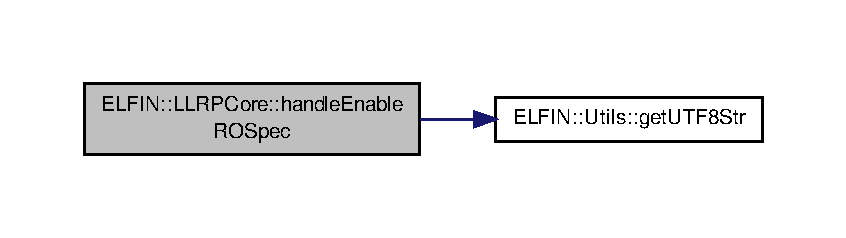
\includegraphics[width=350pt]{class_e_l_f_i_n_1_1_l_l_r_p_core_ade8bc074fb35e9c20d05dfa022bfeac2_cgraph}
\end{center}
\end{figure}


\hypertarget{class_e_l_f_i_n_1_1_l_l_r_p_core_a0fe9819cb4d6f4f2fe7db92bb9d4c6f7}{\index{E\-L\-F\-I\-N\-::\-L\-L\-R\-P\-Core@{E\-L\-F\-I\-N\-::\-L\-L\-R\-P\-Core}!handle\-Get\-Access\-Specs@{handle\-Get\-Access\-Specs}}
\index{handle\-Get\-Access\-Specs@{handle\-Get\-Access\-Specs}!ELFIN::LLRPCore@{E\-L\-F\-I\-N\-::\-L\-L\-R\-P\-Core}}
\subsubsection[{handle\-Get\-Access\-Specs}]{\setlength{\rightskip}{0pt plus 5cm}int E\-L\-F\-I\-N\-::\-L\-L\-R\-P\-Core\-::handle\-Get\-Access\-Specs (
\begin{DoxyParamCaption}
\item[{L\-L\-R\-P\-::\-C\-Message $\ast$}]{\-\_\-p\-Cmd, }
\item[{L\-L\-R\-P\-::\-C\-Message $\ast$$\ast$}]{\-\_\-p\-Rsp}
\end{DoxyParamCaption}
)\hspace{0.3cm}{\ttfamily [private]}}}\label{class_e_l_f_i_n_1_1_l_l_r_p_core_a0fe9819cb4d6f4f2fe7db92bb9d4c6f7}


L\-L\-R\-P message handler method. 



Definition at line 742 of file L\-L\-R\-P\-Core.\-cpp.

\hypertarget{class_e_l_f_i_n_1_1_l_l_r_p_core_a6513619f9917762db82e6b145edada6d}{\index{E\-L\-F\-I\-N\-::\-L\-L\-R\-P\-Core@{E\-L\-F\-I\-N\-::\-L\-L\-R\-P\-Core}!handle\-Get\-Reader\-Capabilities@{handle\-Get\-Reader\-Capabilities}}
\index{handle\-Get\-Reader\-Capabilities@{handle\-Get\-Reader\-Capabilities}!ELFIN::LLRPCore@{E\-L\-F\-I\-N\-::\-L\-L\-R\-P\-Core}}
\subsubsection[{handle\-Get\-Reader\-Capabilities}]{\setlength{\rightskip}{0pt plus 5cm}int E\-L\-F\-I\-N\-::\-L\-L\-R\-P\-Core\-::handle\-Get\-Reader\-Capabilities (
\begin{DoxyParamCaption}
\item[{L\-L\-R\-P\-::\-C\-Message $\ast$}]{\-\_\-p\-Cmd, }
\item[{L\-L\-R\-P\-::\-C\-Message $\ast$$\ast$}]{\-\_\-p\-Rsp}
\end{DoxyParamCaption}
)\hspace{0.3cm}{\ttfamily [private]}}}\label{class_e_l_f_i_n_1_1_l_l_r_p_core_a6513619f9917762db82e6b145edada6d}


L\-L\-R\-P message handler method. 



Definition at line 341 of file L\-L\-R\-P\-Core.\-cpp.



Here is the call graph for this function\-:
\nopagebreak
\begin{figure}[H]
\begin{center}
\leavevmode
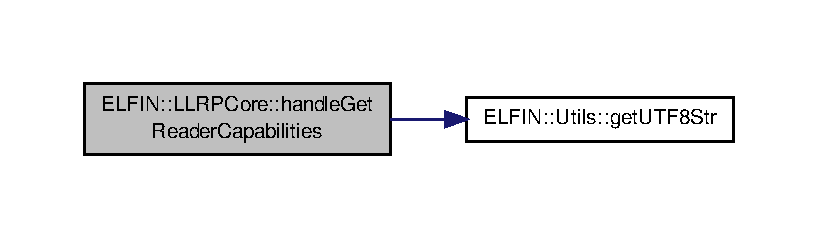
\includegraphics[width=350pt]{class_e_l_f_i_n_1_1_l_l_r_p_core_a6513619f9917762db82e6b145edada6d_cgraph}
\end{center}
\end{figure}


\hypertarget{class_e_l_f_i_n_1_1_l_l_r_p_core_a875e8917fc9f44232d1355f3d91a76e2}{\index{E\-L\-F\-I\-N\-::\-L\-L\-R\-P\-Core@{E\-L\-F\-I\-N\-::\-L\-L\-R\-P\-Core}!handle\-Get\-Reader\-Config@{handle\-Get\-Reader\-Config}}
\index{handle\-Get\-Reader\-Config@{handle\-Get\-Reader\-Config}!ELFIN::LLRPCore@{E\-L\-F\-I\-N\-::\-L\-L\-R\-P\-Core}}
\subsubsection[{handle\-Get\-Reader\-Config}]{\setlength{\rightskip}{0pt plus 5cm}int E\-L\-F\-I\-N\-::\-L\-L\-R\-P\-Core\-::handle\-Get\-Reader\-Config (
\begin{DoxyParamCaption}
\item[{L\-L\-R\-P\-::\-C\-Message $\ast$}]{\-\_\-p\-Cmd, }
\item[{L\-L\-R\-P\-::\-C\-Message $\ast$$\ast$}]{\-\_\-p\-Rsp}
\end{DoxyParamCaption}
)\hspace{0.3cm}{\ttfamily [private]}}}\label{class_e_l_f_i_n_1_1_l_l_r_p_core_a875e8917fc9f44232d1355f3d91a76e2}


L\-L\-R\-P message handler method. 



Definition at line 773 of file L\-L\-R\-P\-Core.\-cpp.



Here is the call graph for this function\-:
\nopagebreak
\begin{figure}[H]
\begin{center}
\leavevmode
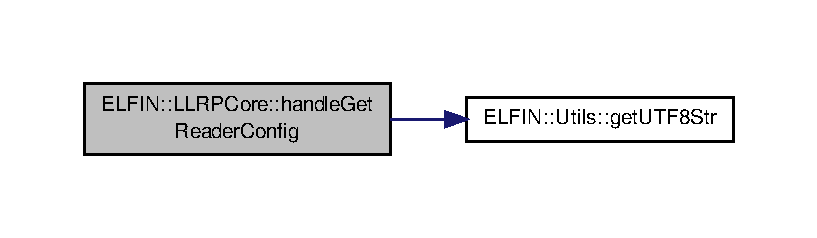
\includegraphics[width=350pt]{class_e_l_f_i_n_1_1_l_l_r_p_core_a875e8917fc9f44232d1355f3d91a76e2_cgraph}
\end{center}
\end{figure}


\hypertarget{class_e_l_f_i_n_1_1_l_l_r_p_core_add0b12e57fcac6dd50a862a48a4bf31e}{\index{E\-L\-F\-I\-N\-::\-L\-L\-R\-P\-Core@{E\-L\-F\-I\-N\-::\-L\-L\-R\-P\-Core}!handle\-Get\-R\-O\-Specs@{handle\-Get\-R\-O\-Specs}}
\index{handle\-Get\-R\-O\-Specs@{handle\-Get\-R\-O\-Specs}!ELFIN::LLRPCore@{E\-L\-F\-I\-N\-::\-L\-L\-R\-P\-Core}}
\subsubsection[{handle\-Get\-R\-O\-Specs}]{\setlength{\rightskip}{0pt plus 5cm}int E\-L\-F\-I\-N\-::\-L\-L\-R\-P\-Core\-::handle\-Get\-R\-O\-Specs (
\begin{DoxyParamCaption}
\item[{L\-L\-R\-P\-::\-C\-Message $\ast$}]{\-\_\-p\-Cmd, }
\item[{L\-L\-R\-P\-::\-C\-Message $\ast$$\ast$}]{\-\_\-p\-Rsp}
\end{DoxyParamCaption}
)\hspace{0.3cm}{\ttfamily [private]}}}\label{class_e_l_f_i_n_1_1_l_l_r_p_core_add0b12e57fcac6dd50a862a48a4bf31e}


L\-L\-R\-P message handler method. 



Definition at line 601 of file L\-L\-R\-P\-Core.\-cpp.

\hypertarget{class_e_l_f_i_n_1_1_l_l_r_p_core_a68fc07b9a02e9d81abaf3536d3be2bb3}{\index{E\-L\-F\-I\-N\-::\-L\-L\-R\-P\-Core@{E\-L\-F\-I\-N\-::\-L\-L\-R\-P\-Core}!handle\-Get\-Supported\-Version@{handle\-Get\-Supported\-Version}}
\index{handle\-Get\-Supported\-Version@{handle\-Get\-Supported\-Version}!ELFIN::LLRPCore@{E\-L\-F\-I\-N\-::\-L\-L\-R\-P\-Core}}
\subsubsection[{handle\-Get\-Supported\-Version}]{\setlength{\rightskip}{0pt plus 5cm}int E\-L\-F\-I\-N\-::\-L\-L\-R\-P\-Core\-::handle\-Get\-Supported\-Version (
\begin{DoxyParamCaption}
\item[{L\-L\-R\-P\-::\-C\-Message $\ast$}]{\-\_\-p\-Cmd, }
\item[{L\-L\-R\-P\-::\-C\-Message $\ast$$\ast$}]{\-\_\-p\-Rsp}
\end{DoxyParamCaption}
)\hspace{0.3cm}{\ttfamily [private]}}}\label{class_e_l_f_i_n_1_1_l_l_r_p_core_a68fc07b9a02e9d81abaf3536d3be2bb3}


L\-L\-R\-P message handler method. 



Definition at line 290 of file L\-L\-R\-P\-Core.\-cpp.

\hypertarget{class_e_l_f_i_n_1_1_l_l_r_p_core_a1e32c1a8d11bcf11f5d8143eac90fd91}{\index{E\-L\-F\-I\-N\-::\-L\-L\-R\-P\-Core@{E\-L\-F\-I\-N\-::\-L\-L\-R\-P\-Core}!handle\-Set\-Protocol\-Version@{handle\-Set\-Protocol\-Version}}
\index{handle\-Set\-Protocol\-Version@{handle\-Set\-Protocol\-Version}!ELFIN::LLRPCore@{E\-L\-F\-I\-N\-::\-L\-L\-R\-P\-Core}}
\subsubsection[{handle\-Set\-Protocol\-Version}]{\setlength{\rightskip}{0pt plus 5cm}int E\-L\-F\-I\-N\-::\-L\-L\-R\-P\-Core\-::handle\-Set\-Protocol\-Version (
\begin{DoxyParamCaption}
\item[{L\-L\-R\-P\-::\-C\-Message $\ast$}]{\-\_\-p\-Cmd, }
\item[{L\-L\-R\-P\-::\-C\-Message $\ast$$\ast$}]{\-\_\-p\-Rsp}
\end{DoxyParamCaption}
)\hspace{0.3cm}{\ttfamily [private]}}}\label{class_e_l_f_i_n_1_1_l_l_r_p_core_a1e32c1a8d11bcf11f5d8143eac90fd91}
\begin{DoxyRefDesc}{Todo}
\item[\hyperlink{todo__todo000012}{Todo}]L\-L\-R\-P 1.\-0.\-1 is currently not supported. \end{DoxyRefDesc}


\begin{DoxyRefDesc}{Todo}
\item[\hyperlink{todo__todo000013}{Todo}]If this message comes with same protocol version twice, then L\-L\-R\-P Wrapper should response with M\-\_\-\-Unexpected\-Message. \end{DoxyRefDesc}


Definition at line 311 of file L\-L\-R\-P\-Core.\-cpp.



Here is the call graph for this function\-:
\nopagebreak
\begin{figure}[H]
\begin{center}
\leavevmode
\includegraphics[width=350pt]{class_e_l_f_i_n_1_1_l_l_r_p_core_a1e32c1a8d11bcf11f5d8143eac90fd91_cgraph}
\end{center}
\end{figure}


\hypertarget{class_e_l_f_i_n_1_1_l_l_r_p_core_a0065a7307c4ea46db3fea2cd109bc1e1}{\index{E\-L\-F\-I\-N\-::\-L\-L\-R\-P\-Core@{E\-L\-F\-I\-N\-::\-L\-L\-R\-P\-Core}!handle\-Set\-Reader\-Config@{handle\-Set\-Reader\-Config}}
\index{handle\-Set\-Reader\-Config@{handle\-Set\-Reader\-Config}!ELFIN::LLRPCore@{E\-L\-F\-I\-N\-::\-L\-L\-R\-P\-Core}}
\subsubsection[{handle\-Set\-Reader\-Config}]{\setlength{\rightskip}{0pt plus 5cm}int E\-L\-F\-I\-N\-::\-L\-L\-R\-P\-Core\-::handle\-Set\-Reader\-Config (
\begin{DoxyParamCaption}
\item[{L\-L\-R\-P\-::\-C\-Message $\ast$}]{\-\_\-p\-Cmd, }
\item[{L\-L\-R\-P\-::\-C\-Message $\ast$$\ast$}]{\-\_\-p\-Rsp}
\end{DoxyParamCaption}
)\hspace{0.3cm}{\ttfamily [private]}}}\label{class_e_l_f_i_n_1_1_l_l_r_p_core_a0065a7307c4ea46db3fea2cd109bc1e1}
\begin{DoxyRefDesc}{Todo}
\item[\hyperlink{todo__todo000014}{Todo}]Handle no such G\-P\-O\-Port failure \end{DoxyRefDesc}


Definition at line 966 of file L\-L\-R\-P\-Core.\-cpp.



Here is the call graph for this function\-:
\nopagebreak
\begin{figure}[H]
\begin{center}
\leavevmode
\includegraphics[width=350pt]{class_e_l_f_i_n_1_1_l_l_r_p_core_a0065a7307c4ea46db3fea2cd109bc1e1_cgraph}
\end{center}
\end{figure}


\hypertarget{class_e_l_f_i_n_1_1_l_l_r_p_core_a4b146a62a2a78e1c73862cd3d047c947}{\index{E\-L\-F\-I\-N\-::\-L\-L\-R\-P\-Core@{E\-L\-F\-I\-N\-::\-L\-L\-R\-P\-Core}!handle\-Start\-R\-O\-Spec@{handle\-Start\-R\-O\-Spec}}
\index{handle\-Start\-R\-O\-Spec@{handle\-Start\-R\-O\-Spec}!ELFIN::LLRPCore@{E\-L\-F\-I\-N\-::\-L\-L\-R\-P\-Core}}
\subsubsection[{handle\-Start\-R\-O\-Spec}]{\setlength{\rightskip}{0pt plus 5cm}int E\-L\-F\-I\-N\-::\-L\-L\-R\-P\-Core\-::handle\-Start\-R\-O\-Spec (
\begin{DoxyParamCaption}
\item[{L\-L\-R\-P\-::\-C\-Message $\ast$}]{\-\_\-p\-Cmd, }
\item[{L\-L\-R\-P\-::\-C\-Message $\ast$$\ast$}]{\-\_\-p\-Rsp}
\end{DoxyParamCaption}
)\hspace{0.3cm}{\ttfamily [private]}}}\label{class_e_l_f_i_n_1_1_l_l_r_p_core_a4b146a62a2a78e1c73862cd3d047c947}


L\-L\-R\-P message handler method. 



Definition at line 498 of file L\-L\-R\-P\-Core.\-cpp.



Here is the call graph for this function\-:
\nopagebreak
\begin{figure}[H]
\begin{center}
\leavevmode
\includegraphics[width=350pt]{class_e_l_f_i_n_1_1_l_l_r_p_core_a4b146a62a2a78e1c73862cd3d047c947_cgraph}
\end{center}
\end{figure}


\hypertarget{class_e_l_f_i_n_1_1_l_l_r_p_core_a3de21a966ba229befbbbf0408fe4fc8e}{\index{E\-L\-F\-I\-N\-::\-L\-L\-R\-P\-Core@{E\-L\-F\-I\-N\-::\-L\-L\-R\-P\-Core}!handle\-Stop\-R\-O\-Spec@{handle\-Stop\-R\-O\-Spec}}
\index{handle\-Stop\-R\-O\-Spec@{handle\-Stop\-R\-O\-Spec}!ELFIN::LLRPCore@{E\-L\-F\-I\-N\-::\-L\-L\-R\-P\-Core}}
\subsubsection[{handle\-Stop\-R\-O\-Spec}]{\setlength{\rightskip}{0pt plus 5cm}int E\-L\-F\-I\-N\-::\-L\-L\-R\-P\-Core\-::handle\-Stop\-R\-O\-Spec (
\begin{DoxyParamCaption}
\item[{L\-L\-R\-P\-::\-C\-Message $\ast$}]{\-\_\-p\-Cmd, }
\item[{L\-L\-R\-P\-::\-C\-Message $\ast$$\ast$}]{\-\_\-p\-Rsp}
\end{DoxyParamCaption}
)\hspace{0.3cm}{\ttfamily [private]}}}\label{class_e_l_f_i_n_1_1_l_l_r_p_core_a3de21a966ba229befbbbf0408fe4fc8e}


L\-L\-R\-P message handler method. 



Definition at line 524 of file L\-L\-R\-P\-Core.\-cpp.



Here is the call graph for this function\-:
\nopagebreak
\begin{figure}[H]
\begin{center}
\leavevmode
\includegraphics[width=350pt]{class_e_l_f_i_n_1_1_l_l_r_p_core_a3de21a966ba229befbbbf0408fe4fc8e_cgraph}
\end{center}
\end{figure}


\hypertarget{class_e_l_f_i_n_1_1_l_l_r_p_core_a70f26fde25b719082c2738e816e25438}{\index{E\-L\-F\-I\-N\-::\-L\-L\-R\-P\-Core@{E\-L\-F\-I\-N\-::\-L\-L\-R\-P\-Core}!init@{init}}
\index{init@{init}!ELFIN::LLRPCore@{E\-L\-F\-I\-N\-::\-L\-L\-R\-P\-Core}}
\subsubsection[{init}]{\setlength{\rightskip}{0pt plus 5cm}int E\-L\-F\-I\-N\-::\-L\-L\-R\-P\-Core\-::init (
\begin{DoxyParamCaption}
{}
\end{DoxyParamCaption}
)}}\label{class_e_l_f_i_n_1_1_l_l_r_p_core_a70f26fde25b719082c2738e816e25438}


Initialize \hyperlink{class_e_l_f_i_n_1_1_l_l_r_p_core}{L\-L\-R\-P\-Core} object by setting default values and instantiating all required objects. 



Definition at line 29 of file L\-L\-R\-P\-Core.\-cpp.

\hypertarget{class_e_l_f_i_n_1_1_l_l_r_p_core_a37541d7698fb45e69c96c5d4b864d30a}{\index{E\-L\-F\-I\-N\-::\-L\-L\-R\-P\-Core@{E\-L\-F\-I\-N\-::\-L\-L\-R\-P\-Core}!is\-Connected@{is\-Connected}}
\index{is\-Connected@{is\-Connected}!ELFIN::LLRPCore@{E\-L\-F\-I\-N\-::\-L\-L\-R\-P\-Core}}
\subsubsection[{is\-Connected}]{\setlength{\rightskip}{0pt plus 5cm}int E\-L\-F\-I\-N\-::\-L\-L\-R\-P\-Core\-::is\-Connected (
\begin{DoxyParamCaption}
{}
\end{DoxyParamCaption}
)}}\label{class_e_l_f_i_n_1_1_l_l_r_p_core_a37541d7698fb45e69c96c5d4b864d30a}


Proxy method of \hyperlink{class_e_l_f_i_n_1_1_c_connection_fn_c_mgr_aa27f8bb83349b52dffe670824cfa0e53}{C\-Connection\-Fn\-C\-Mgr\-::is\-Connected}. 



Definition at line 1242 of file L\-L\-R\-P\-Core.\-cpp.

\hypertarget{class_e_l_f_i_n_1_1_l_l_r_p_core_a606a6a467e33b1727e48a283990d0383}{\index{E\-L\-F\-I\-N\-::\-L\-L\-R\-P\-Core@{E\-L\-F\-I\-N\-::\-L\-L\-R\-P\-Core}!load\-Default\-Config\-File@{load\-Default\-Config\-File}}
\index{load\-Default\-Config\-File@{load\-Default\-Config\-File}!ELFIN::LLRPCore@{E\-L\-F\-I\-N\-::\-L\-L\-R\-P\-Core}}
\subsubsection[{load\-Default\-Config\-File}]{\setlength{\rightskip}{0pt plus 5cm}int E\-L\-F\-I\-N\-::\-L\-L\-R\-P\-Core\-::load\-Default\-Config\-File (
\begin{DoxyParamCaption}
{}
\end{DoxyParamCaption}
)}}\label{class_e_l_f_i_n_1_1_l_l_r_p_core_a606a6a467e33b1727e48a283990d0383}


Load default S\-E\-T\-\_\-\-R\-E\-A\-D\-E\-R\-\_\-\-C\-O\-N\-F\-I\-G message from \hyperlink{class_e_l_f_i_n_1_1_l_l_r_p_reader_config}{L\-L\-R\-P\-Reader\-Config} object and apply it to L\-L\-R\-P Wrapper. 



Definition at line 1234 of file L\-L\-R\-P\-Core.\-cpp.

\hypertarget{class_e_l_f_i_n_1_1_l_l_r_p_core_a7fb97667d470bfddac25da751cf8480e}{\index{E\-L\-F\-I\-N\-::\-L\-L\-R\-P\-Core@{E\-L\-F\-I\-N\-::\-L\-L\-R\-P\-Core}!run@{run}}
\index{run@{run}!ELFIN::LLRPCore@{E\-L\-F\-I\-N\-::\-L\-L\-R\-P\-Core}}
\subsubsection[{run}]{\setlength{\rightskip}{0pt plus 5cm}int E\-L\-F\-I\-N\-::\-L\-L\-R\-P\-Core\-::run (
\begin{DoxyParamCaption}
{}
\end{DoxyParamCaption}
)}}\label{class_e_l_f_i_n_1_1_l_l_r_p_core_a7fb97667d470bfddac25da751cf8480e}


Start L\-L\-R\-P Wrapper. Stub\-App should execute this method to run the L\-L\-R\-P Wrapper. 

\begin{DoxyRefDesc}{Todo}
\item[\hyperlink{todo__todo000010}{Todo}]close connection more elegantly. (not using prog\-Opt to get Reader\-Initiated\-Opt) \end{DoxyRefDesc}


\begin{DoxyRefDesc}{Todo}
\item[\hyperlink{todo__todo000011}{Todo}]close connection more elegantly. (not using prog\-Opt to get Reader\-Initiated\-Opt) \end{DoxyRefDesc}


Definition at line 109 of file L\-L\-R\-P\-Core.\-cpp.

\hypertarget{class_e_l_f_i_n_1_1_l_l_r_p_core_abcc0f5f2a372cffaaf1ece1c4397576e}{\index{E\-L\-F\-I\-N\-::\-L\-L\-R\-P\-Core@{E\-L\-F\-I\-N\-::\-L\-L\-R\-P\-Core}!send\-Message@{send\-Message}}
\index{send\-Message@{send\-Message}!ELFIN::LLRPCore@{E\-L\-F\-I\-N\-::\-L\-L\-R\-P\-Core}}
\subsubsection[{send\-Message}]{\setlength{\rightskip}{0pt plus 5cm}int E\-L\-F\-I\-N\-::\-L\-L\-R\-P\-Core\-::send\-Message (
\begin{DoxyParamCaption}
\item[{L\-L\-R\-P\-::\-C\-Message $\ast$}]{\-\_\-\-\_\-p\-Message}
\end{DoxyParamCaption}
)}}\label{class_e_l_f_i_n_1_1_l_l_r_p_core_abcc0f5f2a372cffaaf1ece1c4397576e}


Proxy method of \hyperlink{class_e_l_f_i_n_1_1_c_connection_fn_c_mgr_a48b283f30ddd8c2b0c2ed55e844085f8}{C\-Connection\-Fn\-C\-Mgr\-::send\-Message}. 



Definition at line 1238 of file L\-L\-R\-P\-Core.\-cpp.

\hypertarget{class_e_l_f_i_n_1_1_l_l_r_p_core_a6fe47b7e4999ced885a160f0c1094a56}{\index{E\-L\-F\-I\-N\-::\-L\-L\-R\-P\-Core@{E\-L\-F\-I\-N\-::\-L\-L\-R\-P\-Core}!set\-Log\-Level@{set\-Log\-Level}}
\index{set\-Log\-Level@{set\-Log\-Level}!ELFIN::LLRPCore@{E\-L\-F\-I\-N\-::\-L\-L\-R\-P\-Core}}
\subsubsection[{set\-Log\-Level}]{\setlength{\rightskip}{0pt plus 5cm}void E\-L\-F\-I\-N\-::\-L\-L\-R\-P\-Core\-::set\-Log\-Level (
\begin{DoxyParamCaption}
\item[{enum E\-Log\-Type}]{p\-Log\-Level}
\end{DoxyParamCaption}
)\hspace{0.3cm}{\ttfamily [static]}}}\label{class_e_l_f_i_n_1_1_l_l_r_p_core_a6fe47b7e4999ced885a160f0c1094a56}


Set the log level of L\-L\-R\-P Wrapper. 


\begin{DoxyParams}{Parameters}
{\em p\-Log\-Level} & Log level. (e.\-g. L\-O\-G\-T\-Y\-P\-E\-\_\-\-A\-L\-L) \\
\hline
\end{DoxyParams}
\begin{DoxyRemark}{Remarks}
Log level is as follows,\par
A\-L\-L $>$ T\-R\-A\-C\-E $>$ D\-E\-B\-U\-G $>$ I\-N\-F\-O $>$ W\-A\-R\-N $>$ E\-R\-R\-O\-R $>$ F\-A\-T\-A\-L $>$ O\-F\-F 
\end{DoxyRemark}


Definition at line 1230 of file L\-L\-R\-P\-Core.\-cpp.



Here is the call graph for this function\-:
\nopagebreak
\begin{figure}[H]
\begin{center}
\leavevmode
\includegraphics[width=350pt]{class_e_l_f_i_n_1_1_l_l_r_p_core_a6fe47b7e4999ced885a160f0c1094a56_cgraph}
\end{center}
\end{figure}




Here is the caller graph for this function\-:
\nopagebreak
\begin{figure}[H]
\begin{center}
\leavevmode
\includegraphics[width=350pt]{class_e_l_f_i_n_1_1_l_l_r_p_core_a6fe47b7e4999ced885a160f0c1094a56_icgraph}
\end{center}
\end{figure}


\hypertarget{class_e_l_f_i_n_1_1_l_l_r_p_core_ab35aa971a25103f0e288bf6cdbd198d0}{\index{E\-L\-F\-I\-N\-::\-L\-L\-R\-P\-Core@{E\-L\-F\-I\-N\-::\-L\-L\-R\-P\-Core}!set\-Reader\-Config@{set\-Reader\-Config}}
\index{set\-Reader\-Config@{set\-Reader\-Config}!ELFIN::LLRPCore@{E\-L\-F\-I\-N\-::\-L\-L\-R\-P\-Core}}
\subsubsection[{set\-Reader\-Config}]{\setlength{\rightskip}{0pt plus 5cm}int E\-L\-F\-I\-N\-::\-L\-L\-R\-P\-Core\-::set\-Reader\-Config (
\begin{DoxyParamCaption}
\item[{L\-L\-R\-P\-::\-C\-Message $\ast$}]{p\-Message}
\end{DoxyParamCaption}
)}}\label{class_e_l_f_i_n_1_1_l_l_r_p_core_ab35aa971a25103f0e288bf6cdbd198d0}


Set the configuration of L\-L\-R\-P\-Reader with S\-E\-T\-\_\-\-R\-E\-A\-D\-E\-R\-\_\-\-C\-O\-N\-F\-I\-G message object. 



Definition at line 1217 of file L\-L\-R\-P\-Core.\-cpp.

\hypertarget{class_e_l_f_i_n_1_1_l_l_r_p_core_a96cf0d4f95c33a628b4c7ea358a9c19a}{\index{E\-L\-F\-I\-N\-::\-L\-L\-R\-P\-Core@{E\-L\-F\-I\-N\-::\-L\-L\-R\-P\-Core}!start\-Connection@{start\-Connection}}
\index{start\-Connection@{start\-Connection}!ELFIN::LLRPCore@{E\-L\-F\-I\-N\-::\-L\-L\-R\-P\-Core}}
\subsubsection[{start\-Connection}]{\setlength{\rightskip}{0pt plus 5cm}int E\-L\-F\-I\-N\-::\-L\-L\-R\-P\-Core\-::start\-Connection (
\begin{DoxyParamCaption}
\item[{void}]{}
\end{DoxyParamCaption}
)}}\label{class_e_l_f_i_n_1_1_l_l_r_p_core_a96cf0d4f95c33a628b4c7ea358a9c19a}


Prepare connection to the Fn\-C server. Initiate connection or wait for connection, according to the {\itshape reader\-Initiated} option. 



Definition at line 97 of file L\-L\-R\-P\-Core.\-cpp.



The documentation for this class was generated from the following files\-:\begin{DoxyCompactItemize}
\item 
elfin\-\_\-src/\hyperlink{_l_l_r_p_core_8h}{L\-L\-R\-P\-Core.\-h}\item 
elfin\-\_\-src/\hyperlink{_l_l_r_p_core_8cpp}{L\-L\-R\-P\-Core.\-cpp}\end{DoxyCompactItemize}

\hypertarget{class_e_l_f_i_n_1_1_l_l_r_p_reader_config}{\section{E\-L\-F\-I\-N\-:\-:L\-L\-R\-P\-Reader\-Config Class Reference}
\label{class_e_l_f_i_n_1_1_l_l_r_p_reader_config}\index{E\-L\-F\-I\-N\-::\-L\-L\-R\-P\-Reader\-Config@{E\-L\-F\-I\-N\-::\-L\-L\-R\-P\-Reader\-Config}}
}


Stores default configurations which can be defined with S\-E\-T\-\_\-\-R\-E\-A\-D\-E\-R\-\_\-\-C\-O\-N\-F\-I\-G message.\par
Also, it parses the contents of default config file ({\itshape config.\-llrp}) and stores it as a default configuration.  




{\ttfamily \#include $<$L\-L\-R\-P\-Reader\-\_\-\-Configurations.\-h$>$}

\subsection*{Public Member Functions}
\begin{DoxyCompactItemize}
\item 
\hyperlink{class_e_l_f_i_n_1_1_l_l_r_p_reader_config_a4f55e8679938e946b457a600c7ea5016}{L\-L\-R\-P\-Reader\-Config} (const char $\ast$\-\_\-\-\_\-p\-Config\-File\-Name)
\begin{DoxyCompactList}\small\item\em Constructor of \hyperlink{class_e_l_f_i_n_1_1_l_l_r_p_reader_config}{L\-L\-R\-P\-Reader\-Config} class. \end{DoxyCompactList}\item 
\hyperlink{class_e_l_f_i_n_1_1_l_l_r_p_reader_config_a30a347d49f018e52fa872b6a69e8931d}{$\sim$\-L\-L\-R\-P\-Reader\-Config} ()
\begin{DoxyCompactList}\small\item\em Destructor of \hyperlink{class_e_l_f_i_n_1_1_l_l_r_p_reader_config}{L\-L\-R\-P\-Reader\-Config} class. \end{DoxyCompactList}\item 
int \hyperlink{class_e_l_f_i_n_1_1_l_l_r_p_reader_config_a91159abaa6a11a46528d199b1c7cda70}{init} ()
\begin{DoxyCompactList}\small\item\em Initialize the object by setting default specs, loading default config file, and build config map. \end{DoxyCompactList}\item 
int \hyperlink{class_e_l_f_i_n_1_1_l_l_r_p_reader_config_a4463324245c5a0158e1ab0010e14f1b7}{clear} ()
\begin{DoxyCompactList}\small\item\em Clear all default specs. \end{DoxyCompactList}\item 
int \hyperlink{class_e_l_f_i_n_1_1_l_l_r_p_reader_config_a1cf22a9b6a589946549f9f8ea0722609}{reset\-To\-Factory\-Default} ()
\begin{DoxyCompactList}\small\item\em Clear and re-\/initialize this object. \end{DoxyCompactList}\item 
void \hyperlink{class_e_l_f_i_n_1_1_l_l_r_p_reader_config_a0095d39a3ef2511c0571c429c02c3ce3}{invalidate\-State\-Value} ()
\begin{DoxyCompactList}\small\item\em Change L\-L\-R\-P\-Configuration\-State\-Value randomly. If this value is changed, we can assume that some configuration values have changed. \end{DoxyCompactList}\item 
int \hyperlink{class_e_l_f_i_n_1_1_l_l_r_p_reader_config_aca8c99f935626d94e87f7fe7f9257def}{load\-Default\-Config\-File} ()
\begin{DoxyCompactList}\small\item\em Load, parse, and store the default config file ({\itshape config.\-llrp}) \end{DoxyCompactList}\end{DoxyCompactItemize}
\subsection*{Public Attributes}
\begin{DoxyCompactItemize}
\item 
\hypertarget{class_e_l_f_i_n_1_1_l_l_r_p_reader_config_a8eedf26161181c2ca8df8da811f75fb0}{char $\ast$ {\bfseries \-\_\-p\-Config\-File\-Name}}\label{class_e_l_f_i_n_1_1_l_l_r_p_reader_config_a8eedf26161181c2ca8df8da811f75fb0}

\item 
\hypertarget{class_e_l_f_i_n_1_1_l_l_r_p_reader_config_a0a973a98e996c0f938a73e10c092b8f6}{L\-L\-R\-P\-::\-C\-R\-O\-Report\-Spec $\ast$ {\bfseries \-\_\-p\-Default\-R\-O\-Report\-Spec}}\label{class_e_l_f_i_n_1_1_l_l_r_p_reader_config_a0a973a98e996c0f938a73e10c092b8f6}

\item 
\hypertarget{class_e_l_f_i_n_1_1_l_l_r_p_reader_config_a365badc2a55000ea5e5418f1a0caa2e7}{L\-L\-R\-P\-::\-C\-Access\-Report\-Spec $\ast$ {\bfseries \-\_\-p\-Default\-Access\-Report\-Spec}}\label{class_e_l_f_i_n_1_1_l_l_r_p_reader_config_a365badc2a55000ea5e5418f1a0caa2e7}

\item 
\hypertarget{class_e_l_f_i_n_1_1_l_l_r_p_reader_config_a6ddbccd547e9ac044c71e2e5748cda29}{L\-L\-R\-P\-::\-C\-Keepalive\-Spec $\ast$ {\bfseries \-\_\-p\-Default\-Keepalive\-Spec}}\label{class_e_l_f_i_n_1_1_l_l_r_p_reader_config_a6ddbccd547e9ac044c71e2e5748cda29}

\item 
\hypertarget{class_e_l_f_i_n_1_1_l_l_r_p_reader_config_af47f84dedf9c34699e002cf4923cfebe}{L\-L\-R\-P\-::\-C\-Events\-And\-Reports $\ast$ {\bfseries \-\_\-p\-Default\-Events\-And\-Reports}}\label{class_e_l_f_i_n_1_1_l_l_r_p_reader_config_af47f84dedf9c34699e002cf4923cfebe}

\item 
\hypertarget{class_e_l_f_i_n_1_1_l_l_r_p_reader_config_a3ae04ccf93bf633df9a6f9000d00c7aa}{L\-L\-R\-P\-::\-C\-Reader\-Event\-Notification\-Spec $\ast$ {\bfseries \-\_\-p\-Default\-Reader\-Event\-Notification\-Spec}}\label{class_e_l_f_i_n_1_1_l_l_r_p_reader_config_a3ae04ccf93bf633df9a6f9000d00c7aa}

\item 
int \hyperlink{class_e_l_f_i_n_1_1_l_l_r_p_reader_config_a5fee5f1463166944eb78a26d2b39858d}{\-\_\-p\-L\-L\-R\-P\-Configuration\-State\-Value}
\begin{DoxyCompactList}\small\item\em This value is changed randomly, when some configuration value is changed. If this value is changed, we can assume that some configuration values have changed. \end{DoxyCompactList}\item 
int \hyperlink{class_e_l_f_i_n_1_1_l_l_r_p_reader_config_ac956371ce5b8c395bdbf5debf4fe9968}{\-\_\-p\-Event\-Noti\-Array} \mbox{[}E\-V\-E\-N\-T\-\_\-\-N\-O\-T\-I\-\_\-\-K\-I\-N\-D\-\_\-\-C\-O\-U\-N\-T\mbox{]}
\begin{DoxyCompactList}\small\item\em Reader\-Event\-Notification configuration map. \hyperlink{class_e_l_f_i_n_1_1_event_notifier}{Event\-Notifier} refers this map to determine which event should be sent. \end{DoxyCompactList}\item 
L\-L\-R\-P\-::\-C\-Message $\ast$ \hyperlink{class_e_l_f_i_n_1_1_l_l_r_p_reader_config_a1ea5b8b04a69ffaf325a7c989c1cf3af}{\-\_\-p\-Default\-Config}
\begin{DoxyCompactList}\small\item\em Default S\-E\-T\-\_\-\-R\-E\-A\-D\-E\-R\-\_\-\-C\-O\-N\-F\-I\-G message object, which is loaded from default config file ({\itshape config.\-llrp}) \end{DoxyCompactList}\end{DoxyCompactItemize}
\subsection*{Private Member Functions}
\begin{DoxyCompactItemize}
\item 
int \hyperlink{class_e_l_f_i_n_1_1_l_l_r_p_reader_config_a694134666941b94248c9a57082252fc1}{set\-Default\-Specs} ()
\begin{DoxyCompactList}\small\item\em Set the default specs. \end{DoxyCompactList}\item 
int \hyperlink{class_e_l_f_i_n_1_1_l_l_r_p_reader_config_a8ecdc94d9c07bf1ede23093618b0f836}{build\-Config\-Maps} ()
\begin{DoxyCompactList}\small\item\em Build Reader\-Event\-Notification configuration map for \hyperlink{class_e_l_f_i_n_1_1_event_notifier}{Event\-Notifier}. \end{DoxyCompactList}\end{DoxyCompactItemize}


\subsection{Detailed Description}
Stores default configurations which can be defined with S\-E\-T\-\_\-\-R\-E\-A\-D\-E\-R\-\_\-\-C\-O\-N\-F\-I\-G message.\par
Also, it parses the contents of default config file ({\itshape config.\-llrp}) and stores it as a default configuration. 

Definition at line 15 of file L\-L\-R\-P\-Reader\-\_\-\-Configurations.\-h.



\subsection{Constructor \& Destructor Documentation}
\hypertarget{class_e_l_f_i_n_1_1_l_l_r_p_reader_config_a4f55e8679938e946b457a600c7ea5016}{\index{E\-L\-F\-I\-N\-::\-L\-L\-R\-P\-Reader\-Config@{E\-L\-F\-I\-N\-::\-L\-L\-R\-P\-Reader\-Config}!L\-L\-R\-P\-Reader\-Config@{L\-L\-R\-P\-Reader\-Config}}
\index{L\-L\-R\-P\-Reader\-Config@{L\-L\-R\-P\-Reader\-Config}!ELFIN::LLRPReaderConfig@{E\-L\-F\-I\-N\-::\-L\-L\-R\-P\-Reader\-Config}}
\subsubsection[{L\-L\-R\-P\-Reader\-Config}]{\setlength{\rightskip}{0pt plus 5cm}E\-L\-F\-I\-N\-::\-L\-L\-R\-P\-Reader\-Config\-::\-L\-L\-R\-P\-Reader\-Config (
\begin{DoxyParamCaption}
\item[{const char $\ast$}]{\-\_\-\-\_\-p\-Config\-File\-Name}
\end{DoxyParamCaption}
)}}\label{class_e_l_f_i_n_1_1_l_l_r_p_reader_config_a4f55e8679938e946b457a600c7ea5016}


Constructor of \hyperlink{class_e_l_f_i_n_1_1_l_l_r_p_reader_config}{L\-L\-R\-P\-Reader\-Config} class. 



Definition at line 12 of file L\-L\-R\-P\-Reader\-\_\-\-Configurations.\-cpp.



Here is the call graph for this function\-:
\nopagebreak
\begin{figure}[H]
\begin{center}
\leavevmode
\includegraphics[width=350pt]{class_e_l_f_i_n_1_1_l_l_r_p_reader_config_a4f55e8679938e946b457a600c7ea5016_cgraph}
\end{center}
\end{figure}


\hypertarget{class_e_l_f_i_n_1_1_l_l_r_p_reader_config_a30a347d49f018e52fa872b6a69e8931d}{\index{E\-L\-F\-I\-N\-::\-L\-L\-R\-P\-Reader\-Config@{E\-L\-F\-I\-N\-::\-L\-L\-R\-P\-Reader\-Config}!$\sim$\-L\-L\-R\-P\-Reader\-Config@{$\sim$\-L\-L\-R\-P\-Reader\-Config}}
\index{$\sim$\-L\-L\-R\-P\-Reader\-Config@{$\sim$\-L\-L\-R\-P\-Reader\-Config}!ELFIN::LLRPReaderConfig@{E\-L\-F\-I\-N\-::\-L\-L\-R\-P\-Reader\-Config}}
\subsubsection[{$\sim$\-L\-L\-R\-P\-Reader\-Config}]{\setlength{\rightskip}{0pt plus 5cm}E\-L\-F\-I\-N\-::\-L\-L\-R\-P\-Reader\-Config\-::$\sim$\-L\-L\-R\-P\-Reader\-Config (
\begin{DoxyParamCaption}
{}
\end{DoxyParamCaption}
)}}\label{class_e_l_f_i_n_1_1_l_l_r_p_reader_config_a30a347d49f018e52fa872b6a69e8931d}


Destructor of \hyperlink{class_e_l_f_i_n_1_1_l_l_r_p_reader_config}{L\-L\-R\-P\-Reader\-Config} class. 



Definition at line 59 of file L\-L\-R\-P\-Reader\-\_\-\-Configurations.\-cpp.



\subsection{Member Function Documentation}
\hypertarget{class_e_l_f_i_n_1_1_l_l_r_p_reader_config_a8ecdc94d9c07bf1ede23093618b0f836}{\index{E\-L\-F\-I\-N\-::\-L\-L\-R\-P\-Reader\-Config@{E\-L\-F\-I\-N\-::\-L\-L\-R\-P\-Reader\-Config}!build\-Config\-Maps@{build\-Config\-Maps}}
\index{build\-Config\-Maps@{build\-Config\-Maps}!ELFIN::LLRPReaderConfig@{E\-L\-F\-I\-N\-::\-L\-L\-R\-P\-Reader\-Config}}
\subsubsection[{build\-Config\-Maps}]{\setlength{\rightskip}{0pt plus 5cm}int E\-L\-F\-I\-N\-::\-L\-L\-R\-P\-Reader\-Config\-::build\-Config\-Maps (
\begin{DoxyParamCaption}
{}
\end{DoxyParamCaption}
)\hspace{0.3cm}{\ttfamily [private]}}}\label{class_e_l_f_i_n_1_1_l_l_r_p_reader_config_a8ecdc94d9c07bf1ede23093618b0f836}


Build Reader\-Event\-Notification configuration map for \hyperlink{class_e_l_f_i_n_1_1_event_notifier}{Event\-Notifier}. 



Definition at line 222 of file L\-L\-R\-P\-Reader\-\_\-\-Configurations.\-cpp.

\hypertarget{class_e_l_f_i_n_1_1_l_l_r_p_reader_config_a4463324245c5a0158e1ab0010e14f1b7}{\index{E\-L\-F\-I\-N\-::\-L\-L\-R\-P\-Reader\-Config@{E\-L\-F\-I\-N\-::\-L\-L\-R\-P\-Reader\-Config}!clear@{clear}}
\index{clear@{clear}!ELFIN::LLRPReaderConfig@{E\-L\-F\-I\-N\-::\-L\-L\-R\-P\-Reader\-Config}}
\subsubsection[{clear}]{\setlength{\rightskip}{0pt plus 5cm}int E\-L\-F\-I\-N\-::\-L\-L\-R\-P\-Reader\-Config\-::clear (
\begin{DoxyParamCaption}
{}
\end{DoxyParamCaption}
)}}\label{class_e_l_f_i_n_1_1_l_l_r_p_reader_config_a4463324245c5a0158e1ab0010e14f1b7}


Clear all default specs. 



Definition at line 22 of file L\-L\-R\-P\-Reader\-\_\-\-Configurations.\-cpp.

\hypertarget{class_e_l_f_i_n_1_1_l_l_r_p_reader_config_a91159abaa6a11a46528d199b1c7cda70}{\index{E\-L\-F\-I\-N\-::\-L\-L\-R\-P\-Reader\-Config@{E\-L\-F\-I\-N\-::\-L\-L\-R\-P\-Reader\-Config}!init@{init}}
\index{init@{init}!ELFIN::LLRPReaderConfig@{E\-L\-F\-I\-N\-::\-L\-L\-R\-P\-Reader\-Config}}
\subsubsection[{init}]{\setlength{\rightskip}{0pt plus 5cm}int E\-L\-F\-I\-N\-::\-L\-L\-R\-P\-Reader\-Config\-::init (
\begin{DoxyParamCaption}
{}
\end{DoxyParamCaption}
)}}\label{class_e_l_f_i_n_1_1_l_l_r_p_reader_config_a91159abaa6a11a46528d199b1c7cda70}


Initialize the object by setting default specs, loading default config file, and build config map. 



Definition at line 64 of file L\-L\-R\-P\-Reader\-\_\-\-Configurations.\-cpp.



Here is the caller graph for this function\-:
\nopagebreak
\begin{figure}[H]
\begin{center}
\leavevmode
\includegraphics[width=350pt]{class_e_l_f_i_n_1_1_l_l_r_p_reader_config_a91159abaa6a11a46528d199b1c7cda70_icgraph}
\end{center}
\end{figure}


\hypertarget{class_e_l_f_i_n_1_1_l_l_r_p_reader_config_a0095d39a3ef2511c0571c429c02c3ce3}{\index{E\-L\-F\-I\-N\-::\-L\-L\-R\-P\-Reader\-Config@{E\-L\-F\-I\-N\-::\-L\-L\-R\-P\-Reader\-Config}!invalidate\-State\-Value@{invalidate\-State\-Value}}
\index{invalidate\-State\-Value@{invalidate\-State\-Value}!ELFIN::LLRPReaderConfig@{E\-L\-F\-I\-N\-::\-L\-L\-R\-P\-Reader\-Config}}
\subsubsection[{invalidate\-State\-Value}]{\setlength{\rightskip}{0pt plus 5cm}void E\-L\-F\-I\-N\-::\-L\-L\-R\-P\-Reader\-Config\-::invalidate\-State\-Value (
\begin{DoxyParamCaption}
{}
\end{DoxyParamCaption}
)}}\label{class_e_l_f_i_n_1_1_l_l_r_p_reader_config_a0095d39a3ef2511c0571c429c02c3ce3}


Change L\-L\-R\-P\-Configuration\-State\-Value randomly. If this value is changed, we can assume that some configuration values have changed. 



Definition at line 238 of file L\-L\-R\-P\-Reader\-\_\-\-Configurations.\-cpp.

\hypertarget{class_e_l_f_i_n_1_1_l_l_r_p_reader_config_aca8c99f935626d94e87f7fe7f9257def}{\index{E\-L\-F\-I\-N\-::\-L\-L\-R\-P\-Reader\-Config@{E\-L\-F\-I\-N\-::\-L\-L\-R\-P\-Reader\-Config}!load\-Default\-Config\-File@{load\-Default\-Config\-File}}
\index{load\-Default\-Config\-File@{load\-Default\-Config\-File}!ELFIN::LLRPReaderConfig@{E\-L\-F\-I\-N\-::\-L\-L\-R\-P\-Reader\-Config}}
\subsubsection[{load\-Default\-Config\-File}]{\setlength{\rightskip}{0pt plus 5cm}int E\-L\-F\-I\-N\-::\-L\-L\-R\-P\-Reader\-Config\-::load\-Default\-Config\-File (
\begin{DoxyParamCaption}
{}
\end{DoxyParamCaption}
)}}\label{class_e_l_f_i_n_1_1_l_l_r_p_reader_config_aca8c99f935626d94e87f7fe7f9257def}


Load, parse, and store the default config file ({\itshape config.\-llrp}) 



Definition at line 75 of file L\-L\-R\-P\-Reader\-\_\-\-Configurations.\-cpp.

\hypertarget{class_e_l_f_i_n_1_1_l_l_r_p_reader_config_a1cf22a9b6a589946549f9f8ea0722609}{\index{E\-L\-F\-I\-N\-::\-L\-L\-R\-P\-Reader\-Config@{E\-L\-F\-I\-N\-::\-L\-L\-R\-P\-Reader\-Config}!reset\-To\-Factory\-Default@{reset\-To\-Factory\-Default}}
\index{reset\-To\-Factory\-Default@{reset\-To\-Factory\-Default}!ELFIN::LLRPReaderConfig@{E\-L\-F\-I\-N\-::\-L\-L\-R\-P\-Reader\-Config}}
\subsubsection[{reset\-To\-Factory\-Default}]{\setlength{\rightskip}{0pt plus 5cm}int E\-L\-F\-I\-N\-::\-L\-L\-R\-P\-Reader\-Config\-::reset\-To\-Factory\-Default (
\begin{DoxyParamCaption}
{}
\end{DoxyParamCaption}
)}}\label{class_e_l_f_i_n_1_1_l_l_r_p_reader_config_a1cf22a9b6a589946549f9f8ea0722609}


Clear and re-\/initialize this object. 



Definition at line 138 of file L\-L\-R\-P\-Reader\-\_\-\-Configurations.\-cpp.

\hypertarget{class_e_l_f_i_n_1_1_l_l_r_p_reader_config_a694134666941b94248c9a57082252fc1}{\index{E\-L\-F\-I\-N\-::\-L\-L\-R\-P\-Reader\-Config@{E\-L\-F\-I\-N\-::\-L\-L\-R\-P\-Reader\-Config}!set\-Default\-Specs@{set\-Default\-Specs}}
\index{set\-Default\-Specs@{set\-Default\-Specs}!ELFIN::LLRPReaderConfig@{E\-L\-F\-I\-N\-::\-L\-L\-R\-P\-Reader\-Config}}
\subsubsection[{set\-Default\-Specs}]{\setlength{\rightskip}{0pt plus 5cm}int E\-L\-F\-I\-N\-::\-L\-L\-R\-P\-Reader\-Config\-::set\-Default\-Specs (
\begin{DoxyParamCaption}
{}
\end{DoxyParamCaption}
)\hspace{0.3cm}{\ttfamily [private]}}}\label{class_e_l_f_i_n_1_1_l_l_r_p_reader_config_a694134666941b94248c9a57082252fc1}


Set the default specs. 



Definition at line 144 of file L\-L\-R\-P\-Reader\-\_\-\-Configurations.\-cpp.



\subsection{Member Data Documentation}
\hypertarget{class_e_l_f_i_n_1_1_l_l_r_p_reader_config_a1ea5b8b04a69ffaf325a7c989c1cf3af}{\index{E\-L\-F\-I\-N\-::\-L\-L\-R\-P\-Reader\-Config@{E\-L\-F\-I\-N\-::\-L\-L\-R\-P\-Reader\-Config}!\-\_\-p\-Default\-Config@{\-\_\-p\-Default\-Config}}
\index{\-\_\-p\-Default\-Config@{\-\_\-p\-Default\-Config}!ELFIN::LLRPReaderConfig@{E\-L\-F\-I\-N\-::\-L\-L\-R\-P\-Reader\-Config}}
\subsubsection[{\-\_\-p\-Default\-Config}]{\setlength{\rightskip}{0pt plus 5cm}L\-L\-R\-P\-::\-C\-Message$\ast$ E\-L\-F\-I\-N\-::\-L\-L\-R\-P\-Reader\-Config\-::\-\_\-p\-Default\-Config}}\label{class_e_l_f_i_n_1_1_l_l_r_p_reader_config_a1ea5b8b04a69ffaf325a7c989c1cf3af}


Default S\-E\-T\-\_\-\-R\-E\-A\-D\-E\-R\-\_\-\-C\-O\-N\-F\-I\-G message object, which is loaded from default config file ({\itshape config.\-llrp}) 



Definition at line 53 of file L\-L\-R\-P\-Reader\-\_\-\-Configurations.\-h.

\hypertarget{class_e_l_f_i_n_1_1_l_l_r_p_reader_config_ac956371ce5b8c395bdbf5debf4fe9968}{\index{E\-L\-F\-I\-N\-::\-L\-L\-R\-P\-Reader\-Config@{E\-L\-F\-I\-N\-::\-L\-L\-R\-P\-Reader\-Config}!\-\_\-p\-Event\-Noti\-Array@{\-\_\-p\-Event\-Noti\-Array}}
\index{\-\_\-p\-Event\-Noti\-Array@{\-\_\-p\-Event\-Noti\-Array}!ELFIN::LLRPReaderConfig@{E\-L\-F\-I\-N\-::\-L\-L\-R\-P\-Reader\-Config}}
\subsubsection[{\-\_\-p\-Event\-Noti\-Array}]{\setlength{\rightskip}{0pt plus 5cm}int E\-L\-F\-I\-N\-::\-L\-L\-R\-P\-Reader\-Config\-::\-\_\-p\-Event\-Noti\-Array\mbox{[}E\-V\-E\-N\-T\-\_\-\-N\-O\-T\-I\-\_\-\-K\-I\-N\-D\-\_\-\-C\-O\-U\-N\-T\mbox{]}}}\label{class_e_l_f_i_n_1_1_l_l_r_p_reader_config_ac956371ce5b8c395bdbf5debf4fe9968}


Reader\-Event\-Notification configuration map. \hyperlink{class_e_l_f_i_n_1_1_event_notifier}{Event\-Notifier} refers this map to determine which event should be sent. 



Definition at line 50 of file L\-L\-R\-P\-Reader\-\_\-\-Configurations.\-h.

\hypertarget{class_e_l_f_i_n_1_1_l_l_r_p_reader_config_a5fee5f1463166944eb78a26d2b39858d}{\index{E\-L\-F\-I\-N\-::\-L\-L\-R\-P\-Reader\-Config@{E\-L\-F\-I\-N\-::\-L\-L\-R\-P\-Reader\-Config}!\-\_\-p\-L\-L\-R\-P\-Configuration\-State\-Value@{\-\_\-p\-L\-L\-R\-P\-Configuration\-State\-Value}}
\index{\-\_\-p\-L\-L\-R\-P\-Configuration\-State\-Value@{\-\_\-p\-L\-L\-R\-P\-Configuration\-State\-Value}!ELFIN::LLRPReaderConfig@{E\-L\-F\-I\-N\-::\-L\-L\-R\-P\-Reader\-Config}}
\subsubsection[{\-\_\-p\-L\-L\-R\-P\-Configuration\-State\-Value}]{\setlength{\rightskip}{0pt plus 5cm}int E\-L\-F\-I\-N\-::\-L\-L\-R\-P\-Reader\-Config\-::\-\_\-p\-L\-L\-R\-P\-Configuration\-State\-Value}}\label{class_e_l_f_i_n_1_1_l_l_r_p_reader_config_a5fee5f1463166944eb78a26d2b39858d}


This value is changed randomly, when some configuration value is changed. If this value is changed, we can assume that some configuration values have changed. 



Definition at line 48 of file L\-L\-R\-P\-Reader\-\_\-\-Configurations.\-h.



The documentation for this class was generated from the following files\-:\begin{DoxyCompactItemize}
\item 
elfin\-\_\-src/\hyperlink{_l_l_r_p_reader___configurations_8h}{L\-L\-R\-P\-Reader\-\_\-\-Configurations.\-h}\item 
elfin\-\_\-src/\hyperlink{_l_l_r_p_reader___configurations_8cpp}{L\-L\-R\-P\-Reader\-\_\-\-Configurations.\-cpp}\end{DoxyCompactItemize}

\hypertarget{class_e_l_f_i_n_1_1_program_options}{\section{E\-L\-F\-I\-N\-:\-:Program\-Options Class Reference}
\label{class_e_l_f_i_n_1_1_program_options}\index{E\-L\-F\-I\-N\-::\-Program\-Options@{E\-L\-F\-I\-N\-::\-Program\-Options}}
}


Parse the configuration file and store it.  




{\ttfamily \#include $<$E\-L\-F\-I\-N\-\_\-\-Prog\-Opts.\-h$>$}

\subsection*{Public Member Functions}
\begin{DoxyCompactItemize}
\item 
\hyperlink{class_e_l_f_i_n_1_1_program_options_ae9c76cc6526e9e5e9a86406cbf7557ae}{Program\-Options} ()
\begin{DoxyCompactList}\small\item\em Constructor of \hyperlink{class_e_l_f_i_n_1_1_program_options}{Program\-Options} class. \end{DoxyCompactList}\item 
virtual \hyperlink{class_e_l_f_i_n_1_1_program_options_a49087de0dba7f30558b339711e25b244}{$\sim$\-Program\-Options} ()
\begin{DoxyCompactList}\small\item\em Destructor of \hyperlink{class_e_l_f_i_n_1_1_program_options}{Program\-Options} class. \end{DoxyCompactList}\item 
int \hyperlink{class_e_l_f_i_n_1_1_program_options_a0597be1826180e777bcf3aa5ee5192a2}{process\-Cmdline\-Options} (int argc, char $\ast$argv\mbox{[}$\,$\mbox{]})
\begin{DoxyCompactList}\small\item\em Parse the command line and configuration file options, and store them. \end{DoxyCompactList}\item 
\hypertarget{class_e_l_f_i_n_1_1_program_options_afef36c153116f9e303c32393d2f3b9a5}{bool {\bfseries is\-Help\-Option} ()}\label{class_e_l_f_i_n_1_1_program_options_afef36c153116f9e303c32393d2f3b9a5}

\item 
\hypertarget{class_e_l_f_i_n_1_1_program_options_a872d4fcf3d92230f5195095faf6794c4}{void {\bfseries print\-Help} ()}\label{class_e_l_f_i_n_1_1_program_options_a872d4fcf3d92230f5195095faf6794c4}

\item 
void \hyperlink{class_e_l_f_i_n_1_1_program_options_ab7ab803dd5e6e0b1ffa650da4be82dee}{print\-Options} ()
\begin{DoxyCompactList}\small\item\em Print current option values. \end{DoxyCompactList}\end{DoxyCompactItemize}
{\bf }\par
\begin{DoxyCompactItemize}
\item 
int \hyperlink{class_e_l_f_i_n_1_1_program_options_aa230c3fa171bb043cbc5eb8d8735bae9}{get\-Reader\-Initiated\-Opt} ()
\begin{DoxyCompactList}\small\item\em Returns the corresponding option value. \end{DoxyCompactList}\item 
std\-::string \hyperlink{class_e_l_f_i_n_1_1_program_options_a70ff019169c55e71c5d6b4083ffc8acf}{get\-Fn\-C\-Address} ()
\begin{DoxyCompactList}\small\item\em Returns the corresponding option value. \end{DoxyCompactList}\item 
int \hyperlink{class_e_l_f_i_n_1_1_program_options_a862c78cff3445b6c69c982d64c553ed1}{get\-Fn\-C\-Port} ()
\begin{DoxyCompactList}\small\item\em Returns the corresponding option value. \end{DoxyCompactList}\item 
std\-::string \hyperlink{class_e_l_f_i_n_1_1_program_options_ac25f97f994242da0fd2f95e36eee4dda}{get\-E\-P\-C} ()
\begin{DoxyCompactList}\small\item\em Returns the corresponding option value. \end{DoxyCompactList}\item 
int \hyperlink{class_e_l_f_i_n_1_1_program_options_a8db8c8e9f0382d71fc926c42e68c9af6}{get\-Is\-Emulator\-Mode} ()
\begin{DoxyCompactList}\small\item\em Returns the corresponding option value. \end{DoxyCompactList}\item 
int \hyperlink{class_e_l_f_i_n_1_1_program_options_a1cb191c3e34401d0550339ab3b62ac48}{get\-G\-P\-I\-Port\-Count} ()
\begin{DoxyCompactList}\small\item\em Returns the corresponding option value. \end{DoxyCompactList}\item 
int \hyperlink{class_e_l_f_i_n_1_1_program_options_ad60494ff56373efc80912162561a8fa3}{get\-G\-P\-O\-Port\-Count} ()
\begin{DoxyCompactList}\small\item\em Returns the corresponding option value. \end{DoxyCompactList}\item 
int \hyperlink{class_e_l_f_i_n_1_1_program_options_ad8d1d9804bb6c51518f6bb5359d62a8d}{get\-Antenna\-Count} ()
\begin{DoxyCompactList}\small\item\em Returns the corresponding option value. \end{DoxyCompactList}\item 
int \hyperlink{class_e_l_f_i_n_1_1_program_options_a3dcacd2989ebed87eee66765b4133b51}{get\-Read\-Cycle} ()
\begin{DoxyCompactList}\small\item\em Returns the corresponding option value. \end{DoxyCompactList}\item 
int \hyperlink{class_e_l_f_i_n_1_1_program_options_adf1a0c270f3eda0ef0b589c4f765963f}{get\-Virtual\-Tag\-Count} ()
\begin{DoxyCompactList}\small\item\em Returns the corresponding option value. \end{DoxyCompactList}\item 
enum E\-Log\-Type \hyperlink{class_e_l_f_i_n_1_1_program_options_a25118270b4fb86ca2bc98ef9996ce847}{get\-Log\-Level} ()
\begin{DoxyCompactList}\small\item\em Returns the corresponding option value. \end{DoxyCompactList}\item 
std\-::string \hyperlink{class_e_l_f_i_n_1_1_program_options_adbd9e9656083dcf06a0a2b99afab33b7}{get\-L\-L\-R\-P\-File\-Name} ()
\begin{DoxyCompactList}\small\item\em Returns the corresponding option value. \end{DoxyCompactList}\end{DoxyCompactItemize}

\subsection*{Private Attributes}
\begin{DoxyCompactItemize}
\item 
\hypertarget{class_e_l_f_i_n_1_1_program_options_a634928958af27c5c61bec63b1c322ed7}{boost\-::program\-\_\-options\-::variables\-\_\-map {\bfseries \-\_\-vm}}\label{class_e_l_f_i_n_1_1_program_options_a634928958af27c5c61bec63b1c322ed7}

\item 
\hypertarget{class_e_l_f_i_n_1_1_program_options_a61846db95193a0bfac31cbc959b85c5a}{boost\-::program\-\_\-options\-::options\-\_\-description {\bfseries \-\_\-visible\-Desc}}\label{class_e_l_f_i_n_1_1_program_options_a61846db95193a0bfac31cbc959b85c5a}

\end{DoxyCompactItemize}


\subsection{Detailed Description}
Parse the configuration file and store it. 

Definition at line 18 of file E\-L\-F\-I\-N\-\_\-\-Prog\-Opts.\-h.



\subsection{Constructor \& Destructor Documentation}
\hypertarget{class_e_l_f_i_n_1_1_program_options_ae9c76cc6526e9e5e9a86406cbf7557ae}{\index{E\-L\-F\-I\-N\-::\-Program\-Options@{E\-L\-F\-I\-N\-::\-Program\-Options}!Program\-Options@{Program\-Options}}
\index{Program\-Options@{Program\-Options}!ELFIN::ProgramOptions@{E\-L\-F\-I\-N\-::\-Program\-Options}}
\subsubsection[{Program\-Options}]{\setlength{\rightskip}{0pt plus 5cm}E\-L\-F\-I\-N\-::\-Program\-Options\-::\-Program\-Options (
\begin{DoxyParamCaption}
{}
\end{DoxyParamCaption}
)}}\label{class_e_l_f_i_n_1_1_program_options_ae9c76cc6526e9e5e9a86406cbf7557ae}


Constructor of \hyperlink{class_e_l_f_i_n_1_1_program_options}{Program\-Options} class. 



Definition at line 44 of file E\-L\-F\-I\-N\-\_\-\-Prog\-Opts.\-cpp.

\hypertarget{class_e_l_f_i_n_1_1_program_options_a49087de0dba7f30558b339711e25b244}{\index{E\-L\-F\-I\-N\-::\-Program\-Options@{E\-L\-F\-I\-N\-::\-Program\-Options}!$\sim$\-Program\-Options@{$\sim$\-Program\-Options}}
\index{$\sim$\-Program\-Options@{$\sim$\-Program\-Options}!ELFIN::ProgramOptions@{E\-L\-F\-I\-N\-::\-Program\-Options}}
\subsubsection[{$\sim$\-Program\-Options}]{\setlength{\rightskip}{0pt plus 5cm}virtual E\-L\-F\-I\-N\-::\-Program\-Options\-::$\sim$\-Program\-Options (
\begin{DoxyParamCaption}
{}
\end{DoxyParamCaption}
)\hspace{0.3cm}{\ttfamily [inline]}, {\ttfamily [virtual]}}}\label{class_e_l_f_i_n_1_1_program_options_a49087de0dba7f30558b339711e25b244}


Destructor of \hyperlink{class_e_l_f_i_n_1_1_program_options}{Program\-Options} class. 



Definition at line 24 of file E\-L\-F\-I\-N\-\_\-\-Prog\-Opts.\-h.



\subsection{Member Function Documentation}
\hypertarget{class_e_l_f_i_n_1_1_program_options_ad8d1d9804bb6c51518f6bb5359d62a8d}{\index{E\-L\-F\-I\-N\-::\-Program\-Options@{E\-L\-F\-I\-N\-::\-Program\-Options}!get\-Antenna\-Count@{get\-Antenna\-Count}}
\index{get\-Antenna\-Count@{get\-Antenna\-Count}!ELFIN::ProgramOptions@{E\-L\-F\-I\-N\-::\-Program\-Options}}
\subsubsection[{get\-Antenna\-Count}]{\setlength{\rightskip}{0pt plus 5cm}int E\-L\-F\-I\-N\-::\-Program\-Options\-::get\-Antenna\-Count (
\begin{DoxyParamCaption}
{}
\end{DoxyParamCaption}
)}}\label{class_e_l_f_i_n_1_1_program_options_ad8d1d9804bb6c51518f6bb5359d62a8d}


Returns the corresponding option value. 



Definition at line 372 of file E\-L\-F\-I\-N\-\_\-\-Prog\-Opts.\-cpp.



Here is the caller graph for this function\-:
\nopagebreak
\begin{figure}[H]
\begin{center}
\leavevmode
\includegraphics[width=348pt]{class_e_l_f_i_n_1_1_program_options_ad8d1d9804bb6c51518f6bb5359d62a8d_icgraph}
\end{center}
\end{figure}


\hypertarget{class_e_l_f_i_n_1_1_program_options_ac25f97f994242da0fd2f95e36eee4dda}{\index{E\-L\-F\-I\-N\-::\-Program\-Options@{E\-L\-F\-I\-N\-::\-Program\-Options}!get\-E\-P\-C@{get\-E\-P\-C}}
\index{get\-E\-P\-C@{get\-E\-P\-C}!ELFIN::ProgramOptions@{E\-L\-F\-I\-N\-::\-Program\-Options}}
\subsubsection[{get\-E\-P\-C}]{\setlength{\rightskip}{0pt plus 5cm}std\-::string E\-L\-F\-I\-N\-::\-Program\-Options\-::get\-E\-P\-C (
\begin{DoxyParamCaption}
{}
\end{DoxyParamCaption}
)}}\label{class_e_l_f_i_n_1_1_program_options_ac25f97f994242da0fd2f95e36eee4dda}


Returns the corresponding option value. 



Definition at line 290 of file E\-L\-F\-I\-N\-\_\-\-Prog\-Opts.\-cpp.



Here is the caller graph for this function\-:
\nopagebreak
\begin{figure}[H]
\begin{center}
\leavevmode
\includegraphics[width=348pt]{class_e_l_f_i_n_1_1_program_options_ac25f97f994242da0fd2f95e36eee4dda_icgraph}
\end{center}
\end{figure}


\hypertarget{class_e_l_f_i_n_1_1_program_options_a70ff019169c55e71c5d6b4083ffc8acf}{\index{E\-L\-F\-I\-N\-::\-Program\-Options@{E\-L\-F\-I\-N\-::\-Program\-Options}!get\-Fn\-C\-Address@{get\-Fn\-C\-Address}}
\index{get\-Fn\-C\-Address@{get\-Fn\-C\-Address}!ELFIN::ProgramOptions@{E\-L\-F\-I\-N\-::\-Program\-Options}}
\subsubsection[{get\-Fn\-C\-Address}]{\setlength{\rightskip}{0pt plus 5cm}std\-::string E\-L\-F\-I\-N\-::\-Program\-Options\-::get\-Fn\-C\-Address (
\begin{DoxyParamCaption}
{}
\end{DoxyParamCaption}
)}}\label{class_e_l_f_i_n_1_1_program_options_a70ff019169c55e71c5d6b4083ffc8acf}


Returns the corresponding option value. 



Definition at line 255 of file E\-L\-F\-I\-N\-\_\-\-Prog\-Opts.\-cpp.



Here is the caller graph for this function\-:
\nopagebreak
\begin{figure}[H]
\begin{center}
\leavevmode
\includegraphics[width=350pt]{class_e_l_f_i_n_1_1_program_options_a70ff019169c55e71c5d6b4083ffc8acf_icgraph}
\end{center}
\end{figure}


\hypertarget{class_e_l_f_i_n_1_1_program_options_a862c78cff3445b6c69c982d64c553ed1}{\index{E\-L\-F\-I\-N\-::\-Program\-Options@{E\-L\-F\-I\-N\-::\-Program\-Options}!get\-Fn\-C\-Port@{get\-Fn\-C\-Port}}
\index{get\-Fn\-C\-Port@{get\-Fn\-C\-Port}!ELFIN::ProgramOptions@{E\-L\-F\-I\-N\-::\-Program\-Options}}
\subsubsection[{get\-Fn\-C\-Port}]{\setlength{\rightskip}{0pt plus 5cm}int E\-L\-F\-I\-N\-::\-Program\-Options\-::get\-Fn\-C\-Port (
\begin{DoxyParamCaption}
{}
\end{DoxyParamCaption}
)}}\label{class_e_l_f_i_n_1_1_program_options_a862c78cff3445b6c69c982d64c553ed1}


Returns the corresponding option value. 



Definition at line 271 of file E\-L\-F\-I\-N\-\_\-\-Prog\-Opts.\-cpp.



Here is the caller graph for this function\-:
\nopagebreak
\begin{figure}[H]
\begin{center}
\leavevmode
\includegraphics[width=350pt]{class_e_l_f_i_n_1_1_program_options_a862c78cff3445b6c69c982d64c553ed1_icgraph}
\end{center}
\end{figure}


\hypertarget{class_e_l_f_i_n_1_1_program_options_a1cb191c3e34401d0550339ab3b62ac48}{\index{E\-L\-F\-I\-N\-::\-Program\-Options@{E\-L\-F\-I\-N\-::\-Program\-Options}!get\-G\-P\-I\-Port\-Count@{get\-G\-P\-I\-Port\-Count}}
\index{get\-G\-P\-I\-Port\-Count@{get\-G\-P\-I\-Port\-Count}!ELFIN::ProgramOptions@{E\-L\-F\-I\-N\-::\-Program\-Options}}
\subsubsection[{get\-G\-P\-I\-Port\-Count}]{\setlength{\rightskip}{0pt plus 5cm}int E\-L\-F\-I\-N\-::\-Program\-Options\-::get\-G\-P\-I\-Port\-Count (
\begin{DoxyParamCaption}
{}
\end{DoxyParamCaption}
)}}\label{class_e_l_f_i_n_1_1_program_options_a1cb191c3e34401d0550339ab3b62ac48}


Returns the corresponding option value. 



Definition at line 334 of file E\-L\-F\-I\-N\-\_\-\-Prog\-Opts.\-cpp.



Here is the caller graph for this function\-:
\nopagebreak
\begin{figure}[H]
\begin{center}
\leavevmode
\includegraphics[width=348pt]{class_e_l_f_i_n_1_1_program_options_a1cb191c3e34401d0550339ab3b62ac48_icgraph}
\end{center}
\end{figure}


\hypertarget{class_e_l_f_i_n_1_1_program_options_ad60494ff56373efc80912162561a8fa3}{\index{E\-L\-F\-I\-N\-::\-Program\-Options@{E\-L\-F\-I\-N\-::\-Program\-Options}!get\-G\-P\-O\-Port\-Count@{get\-G\-P\-O\-Port\-Count}}
\index{get\-G\-P\-O\-Port\-Count@{get\-G\-P\-O\-Port\-Count}!ELFIN::ProgramOptions@{E\-L\-F\-I\-N\-::\-Program\-Options}}
\subsubsection[{get\-G\-P\-O\-Port\-Count}]{\setlength{\rightskip}{0pt plus 5cm}int E\-L\-F\-I\-N\-::\-Program\-Options\-::get\-G\-P\-O\-Port\-Count (
\begin{DoxyParamCaption}
{}
\end{DoxyParamCaption}
)}}\label{class_e_l_f_i_n_1_1_program_options_ad60494ff56373efc80912162561a8fa3}


Returns the corresponding option value. 



Definition at line 352 of file E\-L\-F\-I\-N\-\_\-\-Prog\-Opts.\-cpp.



Here is the caller graph for this function\-:
\nopagebreak
\begin{figure}[H]
\begin{center}
\leavevmode
\includegraphics[width=348pt]{class_e_l_f_i_n_1_1_program_options_ad60494ff56373efc80912162561a8fa3_icgraph}
\end{center}
\end{figure}


\hypertarget{class_e_l_f_i_n_1_1_program_options_a8db8c8e9f0382d71fc926c42e68c9af6}{\index{E\-L\-F\-I\-N\-::\-Program\-Options@{E\-L\-F\-I\-N\-::\-Program\-Options}!get\-Is\-Emulator\-Mode@{get\-Is\-Emulator\-Mode}}
\index{get\-Is\-Emulator\-Mode@{get\-Is\-Emulator\-Mode}!ELFIN::ProgramOptions@{E\-L\-F\-I\-N\-::\-Program\-Options}}
\subsubsection[{get\-Is\-Emulator\-Mode}]{\setlength{\rightskip}{0pt plus 5cm}int E\-L\-F\-I\-N\-::\-Program\-Options\-::get\-Is\-Emulator\-Mode (
\begin{DoxyParamCaption}
{}
\end{DoxyParamCaption}
)}}\label{class_e_l_f_i_n_1_1_program_options_a8db8c8e9f0382d71fc926c42e68c9af6}


Returns the corresponding option value. 



Definition at line 306 of file E\-L\-F\-I\-N\-\_\-\-Prog\-Opts.\-cpp.



Here is the caller graph for this function\-:
\nopagebreak
\begin{figure}[H]
\begin{center}
\leavevmode
\includegraphics[width=348pt]{class_e_l_f_i_n_1_1_program_options_a8db8c8e9f0382d71fc926c42e68c9af6_icgraph}
\end{center}
\end{figure}


\hypertarget{class_e_l_f_i_n_1_1_program_options_adbd9e9656083dcf06a0a2b99afab33b7}{\index{E\-L\-F\-I\-N\-::\-Program\-Options@{E\-L\-F\-I\-N\-::\-Program\-Options}!get\-L\-L\-R\-P\-File\-Name@{get\-L\-L\-R\-P\-File\-Name}}
\index{get\-L\-L\-R\-P\-File\-Name@{get\-L\-L\-R\-P\-File\-Name}!ELFIN::ProgramOptions@{E\-L\-F\-I\-N\-::\-Program\-Options}}
\subsubsection[{get\-L\-L\-R\-P\-File\-Name}]{\setlength{\rightskip}{0pt plus 5cm}std\-::string E\-L\-F\-I\-N\-::\-Program\-Options\-::get\-L\-L\-R\-P\-File\-Name (
\begin{DoxyParamCaption}
{}
\end{DoxyParamCaption}
)}}\label{class_e_l_f_i_n_1_1_program_options_adbd9e9656083dcf06a0a2b99afab33b7}


Returns the corresponding option value. 



Definition at line 426 of file E\-L\-F\-I\-N\-\_\-\-Prog\-Opts.\-cpp.

\hypertarget{class_e_l_f_i_n_1_1_program_options_a25118270b4fb86ca2bc98ef9996ce847}{\index{E\-L\-F\-I\-N\-::\-Program\-Options@{E\-L\-F\-I\-N\-::\-Program\-Options}!get\-Log\-Level@{get\-Log\-Level}}
\index{get\-Log\-Level@{get\-Log\-Level}!ELFIN::ProgramOptions@{E\-L\-F\-I\-N\-::\-Program\-Options}}
\subsubsection[{get\-Log\-Level}]{\setlength{\rightskip}{0pt plus 5cm}enum E\-L\-F\-I\-N\-::\-E\-Log\-Type E\-L\-F\-I\-N\-::\-Program\-Options\-::get\-Log\-Level (
\begin{DoxyParamCaption}
{}
\end{DoxyParamCaption}
)}}\label{class_e_l_f_i_n_1_1_program_options_a25118270b4fb86ca2bc98ef9996ce847}


Returns the corresponding option value. 



Definition at line 442 of file E\-L\-F\-I\-N\-\_\-\-Prog\-Opts.\-cpp.



Here is the caller graph for this function\-:
\nopagebreak
\begin{figure}[H]
\begin{center}
\leavevmode
\includegraphics[width=350pt]{class_e_l_f_i_n_1_1_program_options_a25118270b4fb86ca2bc98ef9996ce847_icgraph}
\end{center}
\end{figure}


\hypertarget{class_e_l_f_i_n_1_1_program_options_a3dcacd2989ebed87eee66765b4133b51}{\index{E\-L\-F\-I\-N\-::\-Program\-Options@{E\-L\-F\-I\-N\-::\-Program\-Options}!get\-Read\-Cycle@{get\-Read\-Cycle}}
\index{get\-Read\-Cycle@{get\-Read\-Cycle}!ELFIN::ProgramOptions@{E\-L\-F\-I\-N\-::\-Program\-Options}}
\subsubsection[{get\-Read\-Cycle}]{\setlength{\rightskip}{0pt plus 5cm}int E\-L\-F\-I\-N\-::\-Program\-Options\-::get\-Read\-Cycle (
\begin{DoxyParamCaption}
{}
\end{DoxyParamCaption}
)}}\label{class_e_l_f_i_n_1_1_program_options_a3dcacd2989ebed87eee66765b4133b51}


Returns the corresponding option value. 



Definition at line 390 of file E\-L\-F\-I\-N\-\_\-\-Prog\-Opts.\-cpp.



Here is the caller graph for this function\-:
\nopagebreak
\begin{figure}[H]
\begin{center}
\leavevmode
\includegraphics[width=348pt]{class_e_l_f_i_n_1_1_program_options_a3dcacd2989ebed87eee66765b4133b51_icgraph}
\end{center}
\end{figure}


\hypertarget{class_e_l_f_i_n_1_1_program_options_aa230c3fa171bb043cbc5eb8d8735bae9}{\index{E\-L\-F\-I\-N\-::\-Program\-Options@{E\-L\-F\-I\-N\-::\-Program\-Options}!get\-Reader\-Initiated\-Opt@{get\-Reader\-Initiated\-Opt}}
\index{get\-Reader\-Initiated\-Opt@{get\-Reader\-Initiated\-Opt}!ELFIN::ProgramOptions@{E\-L\-F\-I\-N\-::\-Program\-Options}}
\subsubsection[{get\-Reader\-Initiated\-Opt}]{\setlength{\rightskip}{0pt plus 5cm}int E\-L\-F\-I\-N\-::\-Program\-Options\-::get\-Reader\-Initiated\-Opt (
\begin{DoxyParamCaption}
{}
\end{DoxyParamCaption}
)}}\label{class_e_l_f_i_n_1_1_program_options_aa230c3fa171bb043cbc5eb8d8735bae9}


Returns the corresponding option value. 



Definition at line 227 of file E\-L\-F\-I\-N\-\_\-\-Prog\-Opts.\-cpp.



Here is the caller graph for this function\-:
\nopagebreak
\begin{figure}[H]
\begin{center}
\leavevmode
\includegraphics[width=350pt]{class_e_l_f_i_n_1_1_program_options_aa230c3fa171bb043cbc5eb8d8735bae9_icgraph}
\end{center}
\end{figure}


\hypertarget{class_e_l_f_i_n_1_1_program_options_adf1a0c270f3eda0ef0b589c4f765963f}{\index{E\-L\-F\-I\-N\-::\-Program\-Options@{E\-L\-F\-I\-N\-::\-Program\-Options}!get\-Virtual\-Tag\-Count@{get\-Virtual\-Tag\-Count}}
\index{get\-Virtual\-Tag\-Count@{get\-Virtual\-Tag\-Count}!ELFIN::ProgramOptions@{E\-L\-F\-I\-N\-::\-Program\-Options}}
\subsubsection[{get\-Virtual\-Tag\-Count}]{\setlength{\rightskip}{0pt plus 5cm}int E\-L\-F\-I\-N\-::\-Program\-Options\-::get\-Virtual\-Tag\-Count (
\begin{DoxyParamCaption}
{}
\end{DoxyParamCaption}
)}}\label{class_e_l_f_i_n_1_1_program_options_adf1a0c270f3eda0ef0b589c4f765963f}


Returns the corresponding option value. 



Definition at line 408 of file E\-L\-F\-I\-N\-\_\-\-Prog\-Opts.\-cpp.



Here is the caller graph for this function\-:
\nopagebreak
\begin{figure}[H]
\begin{center}
\leavevmode
\includegraphics[width=348pt]{class_e_l_f_i_n_1_1_program_options_adf1a0c270f3eda0ef0b589c4f765963f_icgraph}
\end{center}
\end{figure}


\hypertarget{class_e_l_f_i_n_1_1_program_options_ab7ab803dd5e6e0b1ffa650da4be82dee}{\index{E\-L\-F\-I\-N\-::\-Program\-Options@{E\-L\-F\-I\-N\-::\-Program\-Options}!print\-Options@{print\-Options}}
\index{print\-Options@{print\-Options}!ELFIN::ProgramOptions@{E\-L\-F\-I\-N\-::\-Program\-Options}}
\subsubsection[{print\-Options}]{\setlength{\rightskip}{0pt plus 5cm}void E\-L\-F\-I\-N\-::\-Program\-Options\-::print\-Options (
\begin{DoxyParamCaption}
{}
\end{DoxyParamCaption}
)}}\label{class_e_l_f_i_n_1_1_program_options_ab7ab803dd5e6e0b1ffa650da4be82dee}


Print current option values. 



Definition at line 155 of file E\-L\-F\-I\-N\-\_\-\-Prog\-Opts.\-cpp.



Here is the caller graph for this function\-:
\nopagebreak
\begin{figure}[H]
\begin{center}
\leavevmode
\includegraphics[width=350pt]{class_e_l_f_i_n_1_1_program_options_ab7ab803dd5e6e0b1ffa650da4be82dee_icgraph}
\end{center}
\end{figure}


\hypertarget{class_e_l_f_i_n_1_1_program_options_a0597be1826180e777bcf3aa5ee5192a2}{\index{E\-L\-F\-I\-N\-::\-Program\-Options@{E\-L\-F\-I\-N\-::\-Program\-Options}!process\-Cmdline\-Options@{process\-Cmdline\-Options}}
\index{process\-Cmdline\-Options@{process\-Cmdline\-Options}!ELFIN::ProgramOptions@{E\-L\-F\-I\-N\-::\-Program\-Options}}
\subsubsection[{process\-Cmdline\-Options}]{\setlength{\rightskip}{0pt plus 5cm}int E\-L\-F\-I\-N\-::\-Program\-Options\-::process\-Cmdline\-Options (
\begin{DoxyParamCaption}
\item[{int}]{argc, }
\item[{char $\ast$}]{argv\mbox{[}$\,$\mbox{]}}
\end{DoxyParamCaption}
)}}\label{class_e_l_f_i_n_1_1_program_options_a0597be1826180e777bcf3aa5ee5192a2}


Parse the command line and configuration file options, and store them. 

That class is intended to store values of options, and can store values of arbitrary types. Next, the calls to store, parse\-\_\-command\-\_\-line and notify functions cause vm to contain all the options found on the command line.

Definition at line 49 of file E\-L\-F\-I\-N\-\_\-\-Prog\-Opts.\-cpp.



The documentation for this class was generated from the following files\-:\begin{DoxyCompactItemize}
\item 
elfin\-\_\-src/\hyperlink{_e_l_f_i_n___prog_opts_8h}{E\-L\-F\-I\-N\-\_\-\-Prog\-Opts.\-h}\item 
elfin\-\_\-src/\hyperlink{_e_l_f_i_n___prog_opts_8cpp}{E\-L\-F\-I\-N\-\_\-\-Prog\-Opts.\-cpp}\end{DoxyCompactItemize}

\hypertarget{struct_e_l_f_i_n_1_1_sample_reader_1_1reader}{\section{E\-L\-F\-I\-N\-:\-:Sample\-Reader\-:\-:reader Struct Reference}
\label{struct_e_l_f_i_n_1_1_sample_reader_1_1reader}\index{E\-L\-F\-I\-N\-::\-Sample\-Reader\-::reader@{E\-L\-F\-I\-N\-::\-Sample\-Reader\-::reader}}
}


Collaboration diagram for E\-L\-F\-I\-N\-:\-:Sample\-Reader\-:\-:reader\-:
\nopagebreak
\begin{figure}[H]
\begin{center}
\leavevmode
\includegraphics[width=214pt]{struct_e_l_f_i_n_1_1_sample_reader_1_1reader__coll__graph}
\end{center}
\end{figure}
\subsection*{Public Attributes}
\begin{DoxyCompactItemize}
\item 
\hypertarget{struct_e_l_f_i_n_1_1_sample_reader_1_1reader_a77fe9f24ac253d4a711dfc9f79042173}{\hyperlink{struct_e_l_f_i_n_1_1_sample_reader_1_1antenna}{antenna} {\bfseries antennas} \mbox{[}E\-M\-U\-L\-\_\-\-A\-N\-T\-\_\-\-C\-O\-U\-N\-T+1\mbox{]}}\label{struct_e_l_f_i_n_1_1_sample_reader_1_1reader_a77fe9f24ac253d4a711dfc9f79042173}

\end{DoxyCompactItemize}


\subsection{Detailed Description}


Definition at line 30 of file Sample\-Reader.\-h.



The documentation for this struct was generated from the following file\-:\begin{DoxyCompactItemize}
\item 
elfin\-\_\-src/\-Reader\-Handler/Sample\-Reader.\-h\end{DoxyCompactItemize}

\hypertarget{class_reader_app}{\section{Reader\-App Class Reference}
\label{class_reader_app}\index{Reader\-App@{Reader\-App}}
}


Reader application example class. Developers can refer to this class to implement their own reader application.  




{\ttfamily \#include $<$Reader\-App.\-h$>$}



Inheritance diagram for Reader\-App\-:
\nopagebreak
\begin{figure}[H]
\begin{center}
\leavevmode
\includegraphics[width=200pt]{class_reader_app__inherit__graph}
\end{center}
\end{figure}


Collaboration diagram for Reader\-App\-:
\nopagebreak
\begin{figure}[H]
\begin{center}
\leavevmode
\includegraphics[width=350pt]{class_reader_app__coll__graph}
\end{center}
\end{figure}
\subsection*{Public Member Functions}
\begin{DoxyCompactItemize}
\item 
\hyperlink{class_reader_app_a151ab4039b8f25f5f7b27998a5f5c3e1}{Reader\-App} (\hyperlink{class_e_l_f_i_n_1_1_program_options}{E\-L\-F\-I\-N\-::\-Program\-Options} $\ast$\-\_\-\-\_\-prog\-Opt)
\begin{DoxyCompactList}\small\item\em Constructor of \hyperlink{class_reader_app}{Reader\-App} class. \end{DoxyCompactList}\item 
virtual \hyperlink{class_reader_app_a3a4756d7a580f364dd00e7c58c9b1828}{$\sim$\-Reader\-App} ()
\begin{DoxyCompactList}\small\item\em Destructor of \hyperlink{class_reader_app}{Reader\-App} class. \end{DoxyCompactList}\item 
int \hyperlink{class_reader_app_a9c597f4245e523a0261304bb5780b492}{run} ()
\begin{DoxyCompactList}\small\item\em Instantiate L\-L\-R\-P Wrapper and start it. And then, wait for the L\-L\-R\-P Wrapper thread finishes. \end{DoxyCompactList}\item 
int \hyperlink{class_reader_app_aa2ff06a65b426f938a6443ed4fd822be}{stop} ()
\begin{DoxyCompactList}\small\item\em Send stop signal to L\-L\-R\-P Wrapper and wait until it actually finishes. And then, delete L\-L\-R\-P Wrapper. \end{DoxyCompactList}\item 
void \hyperlink{class_reader_app_a9188fcc8bb91a42d0568d9f4fc72c3d3}{initializaion\-Finished\-Callback} ()
\begin{DoxyCompactList}\small\item\em This callback is invoked when the L\-L\-R\-P Wrapper is successfully connected to F\&C server and ready to work. \end{DoxyCompactList}\item 
void \hyperlink{class_reader_app_af303ef50ad88ff71262cc37963720715}{G\-P\-I\-Triggered\-Inventory\-Finished\-Callback} (int p\-R\-O\-Spec\-I\-D, E\-L\-F\-I\-N\-::\-Tag\-Vector $\ast$p\-Reported\-Tag\-Vector)
\begin{DoxyCompactList}\small\item\em This callback is invoked when the R\-O\-Spec with G\-P\-I start trigger finished its operation and sent R\-O\-\_\-\-A\-C\-C\-E\-S\-S\-\_\-\-R\-E\-P\-O\-R\-T. \end{DoxyCompactList}\item 
void \hyperlink{class_reader_app_ae90a98ed653ffa829a7dd3ddff98244b}{Inventory\-Operation\-Finished\-Callback} (int p\-R\-O\-Spec\-I\-D, E\-L\-F\-I\-N\-::\-Tag\-Vector $\ast$p\-Reported\-Tag\-Vector)
\begin{DoxyCompactList}\small\item\em This callback is invoked when the R\-O\-Spec with non-\/\-G\-P\-I start trigger finished its operation and sent R\-O\-\_\-\-A\-C\-C\-E\-S\-S\-\_\-\-R\-E\-P\-O\-R\-T. \end{DoxyCompactList}\item 
void \hyperlink{class_reader_app_a8a2cc18b3a9e771032e763ac170957a2}{notify\-Connection\-Result\-Callback} (int conn\-Result)
\begin{DoxyCompactList}\small\item\em This callback is invoked when the L\-L\-R\-P Wrapper is successfully connected to F\&C server. \end{DoxyCompactList}\item 
void \hyperlink{class_reader_app_a05825232b6db23daff3ffc5e59be2043}{ready\-To\-Connect\-Callback} ()
\begin{DoxyCompactList}\small\item\em This callback is invoked when the L\-L\-R\-P Wrapper is initialized and ready to start connection with F\&C server. \end{DoxyCompactList}\item 
void \hyperlink{class_reader_app_ac6971b9bead2c6f631fbac1c654faa1c}{connection\-Closed\-Callback} ()
\begin{DoxyCompactList}\small\item\em This callback is invoked when the connection to F\&C server is closed and L\-L\-R\-P Wrapper is re-\/initialized. \end{DoxyCompactList}\item 
void \hyperlink{class_reader_app_a8ec4922b19ffc8db003380f7ee3a5fb5}{G\-P\-O\-Event\-Callback} (int port\-Num, int state)
\begin{DoxyCompactList}\small\item\em This callback is invoked when the S\-E\-T\-\_\-\-R\-E\-A\-D\-E\-R\-\_\-\-C\-O\-N\-F\-I\-G message ordered to change G\-P\-O port value. \end{DoxyCompactList}\end{DoxyCompactItemize}
\subsection*{Public Attributes}
\begin{DoxyCompactItemize}
\item 
\hypertarget{class_reader_app_a8802e67d2b33cd5256f2d79246bbd566}{\hyperlink{class_e_l_f_i_n_1_1_program_options}{E\-L\-F\-I\-N\-::\-Program\-Options} $\ast$ {\bfseries m\-\_\-\-Prog\-Opt}}\label{class_reader_app_a8802e67d2b33cd5256f2d79246bbd566}

\item 
\hypertarget{class_reader_app_aef69c77475a3cf4263138c0ba7181d01}{boost\-::thread $\ast$ {\bfseries m\-\_\-\-L\-L\-R\-P\-Reader\-Thread}}\label{class_reader_app_aef69c77475a3cf4263138c0ba7181d01}

\item 
\hypertarget{class_reader_app_a4bd19e376d76a7475db27d2876bf991f}{\hyperlink{class_e_l_f_i_n_1_1_e_l_f_i_n_reader}{E\-L\-F\-I\-N\-::\-E\-L\-F\-I\-N\-Reader} $\ast$ {\bfseries m\-\_\-\-E\-L\-F\-I\-N\-Reader}}\label{class_reader_app_a4bd19e376d76a7475db27d2876bf991f}

\item 
\hypertarget{class_reader_app_a2171d9c371a395a3416dc4467c7f1794}{int {\bfseries m\-\_\-shutdown\-Flag}}\label{class_reader_app_a2171d9c371a395a3416dc4467c7f1794}

\end{DoxyCompactItemize}


\subsection{Detailed Description}
Reader application example class. Developers can refer to this class to implement their own reader application. 

Definition at line 16 of file Reader\-App.\-h.



\subsection{Constructor \& Destructor Documentation}
\hypertarget{class_reader_app_a151ab4039b8f25f5f7b27998a5f5c3e1}{\index{Reader\-App@{Reader\-App}!Reader\-App@{Reader\-App}}
\index{Reader\-App@{Reader\-App}!ReaderApp@{Reader\-App}}
\subsubsection[{Reader\-App}]{\setlength{\rightskip}{0pt plus 5cm}Reader\-App\-::\-Reader\-App (
\begin{DoxyParamCaption}
\item[{{\bf E\-L\-F\-I\-N\-::\-Program\-Options} $\ast$}]{\-\_\-\-\_\-prog\-Opt}
\end{DoxyParamCaption}
)}}\label{class_reader_app_a151ab4039b8f25f5f7b27998a5f5c3e1}


Constructor of \hyperlink{class_reader_app}{Reader\-App} class. 



Definition at line 60 of file Reader\-App.\-cpp.

\hypertarget{class_reader_app_a3a4756d7a580f364dd00e7c58c9b1828}{\index{Reader\-App@{Reader\-App}!$\sim$\-Reader\-App@{$\sim$\-Reader\-App}}
\index{$\sim$\-Reader\-App@{$\sim$\-Reader\-App}!ReaderApp@{Reader\-App}}
\subsubsection[{$\sim$\-Reader\-App}]{\setlength{\rightskip}{0pt plus 5cm}Reader\-App\-::$\sim$\-Reader\-App (
\begin{DoxyParamCaption}
{}
\end{DoxyParamCaption}
)\hspace{0.3cm}{\ttfamily [virtual]}}}\label{class_reader_app_a3a4756d7a580f364dd00e7c58c9b1828}


Destructor of \hyperlink{class_reader_app}{Reader\-App} class. 



Definition at line 65 of file Reader\-App.\-cpp.



Here is the call graph for this function\-:
\nopagebreak
\begin{figure}[H]
\begin{center}
\leavevmode
\includegraphics[width=332pt]{class_reader_app_a3a4756d7a580f364dd00e7c58c9b1828_cgraph}
\end{center}
\end{figure}




\subsection{Member Function Documentation}
\hypertarget{class_reader_app_ac6971b9bead2c6f631fbac1c654faa1c}{\index{Reader\-App@{Reader\-App}!connection\-Closed\-Callback@{connection\-Closed\-Callback}}
\index{connection\-Closed\-Callback@{connection\-Closed\-Callback}!ReaderApp@{Reader\-App}}
\subsubsection[{connection\-Closed\-Callback}]{\setlength{\rightskip}{0pt plus 5cm}void Reader\-App\-::connection\-Closed\-Callback (
\begin{DoxyParamCaption}
{}
\end{DoxyParamCaption}
)\hspace{0.3cm}{\ttfamily [virtual]}}}\label{class_reader_app_ac6971b9bead2c6f631fbac1c654faa1c}


This callback is invoked when the connection to F\&C server is closed and L\-L\-R\-P Wrapper is re-\/initialized. 



Reimplemented from \hyperlink{class_e_l_f_i_n_1_1_stub_reader_app_a772915f831ab5504f76f03cdd9eac65c}{E\-L\-F\-I\-N\-::\-Stub\-Reader\-App}.



Definition at line 133 of file Reader\-App.\-cpp.

\hypertarget{class_reader_app_af303ef50ad88ff71262cc37963720715}{\index{Reader\-App@{Reader\-App}!G\-P\-I\-Triggered\-Inventory\-Finished\-Callback@{G\-P\-I\-Triggered\-Inventory\-Finished\-Callback}}
\index{G\-P\-I\-Triggered\-Inventory\-Finished\-Callback@{G\-P\-I\-Triggered\-Inventory\-Finished\-Callback}!ReaderApp@{Reader\-App}}
\subsubsection[{G\-P\-I\-Triggered\-Inventory\-Finished\-Callback}]{\setlength{\rightskip}{0pt plus 5cm}void Reader\-App\-::\-G\-P\-I\-Triggered\-Inventory\-Finished\-Callback (
\begin{DoxyParamCaption}
\item[{int}]{p\-R\-O\-Spec\-I\-D, }
\item[{E\-L\-F\-I\-N\-::\-Tag\-Vector $\ast$}]{p\-Reported\-Tag\-Vector}
\end{DoxyParamCaption}
)\hspace{0.3cm}{\ttfamily [virtual]}}}\label{class_reader_app_af303ef50ad88ff71262cc37963720715}


This callback is invoked when the R\-O\-Spec with G\-P\-I start trigger finished its operation and sent R\-O\-\_\-\-A\-C\-C\-E\-S\-S\-\_\-\-R\-E\-P\-O\-R\-T. 



Reimplemented from \hyperlink{class_e_l_f_i_n_1_1_stub_reader_app_a735d892b7f4bc81d21076bea419d23cd}{E\-L\-F\-I\-N\-::\-Stub\-Reader\-App}.



Definition at line 107 of file Reader\-App.\-cpp.

\hypertarget{class_reader_app_a8ec4922b19ffc8db003380f7ee3a5fb5}{\index{Reader\-App@{Reader\-App}!G\-P\-O\-Event\-Callback@{G\-P\-O\-Event\-Callback}}
\index{G\-P\-O\-Event\-Callback@{G\-P\-O\-Event\-Callback}!ReaderApp@{Reader\-App}}
\subsubsection[{G\-P\-O\-Event\-Callback}]{\setlength{\rightskip}{0pt plus 5cm}void Reader\-App\-::\-G\-P\-O\-Event\-Callback (
\begin{DoxyParamCaption}
\item[{int}]{port\-Num, }
\item[{int}]{state}
\end{DoxyParamCaption}
)\hspace{0.3cm}{\ttfamily [virtual]}}}\label{class_reader_app_a8ec4922b19ffc8db003380f7ee3a5fb5}


This callback is invoked when the S\-E\-T\-\_\-\-R\-E\-A\-D\-E\-R\-\_\-\-C\-O\-N\-F\-I\-G message ordered to change G\-P\-O port value. 



Reimplemented from \hyperlink{class_e_l_f_i_n_1_1_stub_reader_app_a4cf4f7c31e213da02eab0905c78dd0b1}{E\-L\-F\-I\-N\-::\-Stub\-Reader\-App}.



Definition at line 139 of file Reader\-App.\-cpp.

\hypertarget{class_reader_app_a9188fcc8bb91a42d0568d9f4fc72c3d3}{\index{Reader\-App@{Reader\-App}!initializaion\-Finished\-Callback@{initializaion\-Finished\-Callback}}
\index{initializaion\-Finished\-Callback@{initializaion\-Finished\-Callback}!ReaderApp@{Reader\-App}}
\subsubsection[{initializaion\-Finished\-Callback}]{\setlength{\rightskip}{0pt plus 5cm}void Reader\-App\-::initializaion\-Finished\-Callback (
\begin{DoxyParamCaption}
{}
\end{DoxyParamCaption}
)\hspace{0.3cm}{\ttfamily [virtual]}}}\label{class_reader_app_a9188fcc8bb91a42d0568d9f4fc72c3d3}


This callback is invoked when the L\-L\-R\-P Wrapper is successfully connected to F\&C server and ready to work. 



Reimplemented from \hyperlink{class_e_l_f_i_n_1_1_stub_reader_app_afb38719e5bd42ea03c4cd7d396b24f33}{E\-L\-F\-I\-N\-::\-Stub\-Reader\-App}.



Definition at line 103 of file Reader\-App.\-cpp.

\hypertarget{class_reader_app_ae90a98ed653ffa829a7dd3ddff98244b}{\index{Reader\-App@{Reader\-App}!Inventory\-Operation\-Finished\-Callback@{Inventory\-Operation\-Finished\-Callback}}
\index{Inventory\-Operation\-Finished\-Callback@{Inventory\-Operation\-Finished\-Callback}!ReaderApp@{Reader\-App}}
\subsubsection[{Inventory\-Operation\-Finished\-Callback}]{\setlength{\rightskip}{0pt plus 5cm}void Reader\-App\-::\-Inventory\-Operation\-Finished\-Callback (
\begin{DoxyParamCaption}
\item[{int}]{p\-R\-O\-Spec\-I\-D, }
\item[{E\-L\-F\-I\-N\-::\-Tag\-Vector $\ast$}]{p\-Reported\-Tag\-Vector}
\end{DoxyParamCaption}
)\hspace{0.3cm}{\ttfamily [virtual]}}}\label{class_reader_app_ae90a98ed653ffa829a7dd3ddff98244b}


This callback is invoked when the R\-O\-Spec with non-\/\-G\-P\-I start trigger finished its operation and sent R\-O\-\_\-\-A\-C\-C\-E\-S\-S\-\_\-\-R\-E\-P\-O\-R\-T. 



Reimplemented from \hyperlink{class_e_l_f_i_n_1_1_stub_reader_app_a543e972efc7806cf15338aa21a4c148a}{E\-L\-F\-I\-N\-::\-Stub\-Reader\-App}.



Definition at line 115 of file Reader\-App.\-cpp.

\hypertarget{class_reader_app_a8a2cc18b3a9e771032e763ac170957a2}{\index{Reader\-App@{Reader\-App}!notify\-Connection\-Result\-Callback@{notify\-Connection\-Result\-Callback}}
\index{notify\-Connection\-Result\-Callback@{notify\-Connection\-Result\-Callback}!ReaderApp@{Reader\-App}}
\subsubsection[{notify\-Connection\-Result\-Callback}]{\setlength{\rightskip}{0pt plus 5cm}void Reader\-App\-::notify\-Connection\-Result\-Callback (
\begin{DoxyParamCaption}
\item[{int}]{conn\-Result}
\end{DoxyParamCaption}
)\hspace{0.3cm}{\ttfamily [virtual]}}}\label{class_reader_app_a8a2cc18b3a9e771032e763ac170957a2}


This callback is invoked when the L\-L\-R\-P Wrapper is successfully connected to F\&C server. 



Reimplemented from \hyperlink{class_e_l_f_i_n_1_1_stub_reader_app_ac904a86d2a2e9b2f53d5c241b67426c7}{E\-L\-F\-I\-N\-::\-Stub\-Reader\-App}.



Definition at line 123 of file Reader\-App.\-cpp.

\hypertarget{class_reader_app_a05825232b6db23daff3ffc5e59be2043}{\index{Reader\-App@{Reader\-App}!ready\-To\-Connect\-Callback@{ready\-To\-Connect\-Callback}}
\index{ready\-To\-Connect\-Callback@{ready\-To\-Connect\-Callback}!ReaderApp@{Reader\-App}}
\subsubsection[{ready\-To\-Connect\-Callback}]{\setlength{\rightskip}{0pt plus 5cm}void Reader\-App\-::ready\-To\-Connect\-Callback (
\begin{DoxyParamCaption}
{}
\end{DoxyParamCaption}
)\hspace{0.3cm}{\ttfamily [virtual]}}}\label{class_reader_app_a05825232b6db23daff3ffc5e59be2043}


This callback is invoked when the L\-L\-R\-P Wrapper is initialized and ready to start connection with F\&C server. 



Reimplemented from \hyperlink{class_e_l_f_i_n_1_1_stub_reader_app_abb3f9fb61d1cadf87438e60271ad4bbd}{E\-L\-F\-I\-N\-::\-Stub\-Reader\-App}.



Definition at line 127 of file Reader\-App.\-cpp.

\hypertarget{class_reader_app_a9c597f4245e523a0261304bb5780b492}{\index{Reader\-App@{Reader\-App}!run@{run}}
\index{run@{run}!ReaderApp@{Reader\-App}}
\subsubsection[{run}]{\setlength{\rightskip}{0pt plus 5cm}int Reader\-App\-::run (
\begin{DoxyParamCaption}
{}
\end{DoxyParamCaption}
)}}\label{class_reader_app_a9c597f4245e523a0261304bb5780b492}


Instantiate L\-L\-R\-P Wrapper and start it. And then, wait for the L\-L\-R\-P Wrapper thread finishes. 



Definition at line 73 of file Reader\-App.\-cpp.

\hypertarget{class_reader_app_aa2ff06a65b426f938a6443ed4fd822be}{\index{Reader\-App@{Reader\-App}!stop@{stop}}
\index{stop@{stop}!ReaderApp@{Reader\-App}}
\subsubsection[{stop}]{\setlength{\rightskip}{0pt plus 5cm}int Reader\-App\-::stop (
\begin{DoxyParamCaption}
{}
\end{DoxyParamCaption}
)}}\label{class_reader_app_aa2ff06a65b426f938a6443ed4fd822be}


Send stop signal to L\-L\-R\-P Wrapper and wait until it actually finishes. And then, delete L\-L\-R\-P Wrapper. 



Definition at line 89 of file Reader\-App.\-cpp.



Here is the caller graph for this function\-:
\nopagebreak
\begin{figure}[H]
\begin{center}
\leavevmode
\includegraphics[width=332pt]{class_reader_app_aa2ff06a65b426f938a6443ed4fd822be_icgraph}
\end{center}
\end{figure}




The documentation for this class was generated from the following files\-:\begin{DoxyCompactItemize}
\item 
elfin\-\_\-app/\hyperlink{_reader_app_8h}{Reader\-App.\-h}\item 
elfin\-\_\-app/\hyperlink{_reader_app_8cpp}{Reader\-App.\-cpp}\end{DoxyCompactItemize}

\hypertarget{class_e_l_f_i_n_1_1_reader_operation}{\section{E\-L\-F\-I\-N\-:\-:Reader\-Operation Class Reference}
\label{class_e_l_f_i_n_1_1_reader_operation}\index{E\-L\-F\-I\-N\-::\-Reader\-Operation@{E\-L\-F\-I\-N\-::\-Reader\-Operation}}
}


A single reader operation generated based on the L\-L\-R\-P R\-O\-Spec message.  




{\ttfamily \#include $<$Reader\-Operation.\-h$>$}



Inheritance diagram for E\-L\-F\-I\-N\-:\-:Reader\-Operation\-:
\nopagebreak
\begin{figure}[H]
\begin{center}
\leavevmode
\includegraphics[width=204pt]{class_e_l_f_i_n_1_1_reader_operation__inherit__graph}
\end{center}
\end{figure}


Collaboration diagram for E\-L\-F\-I\-N\-:\-:Reader\-Operation\-:
\nopagebreak
\begin{figure}[H]
\begin{center}
\leavevmode
\includegraphics[width=350pt]{class_e_l_f_i_n_1_1_reader_operation__coll__graph}
\end{center}
\end{figure}
\subsection*{Public Member Functions}
\begin{DoxyCompactItemize}
\item 
\hyperlink{class_e_l_f_i_n_1_1_reader_operation_a0cf397b0aa83e1c5c9df1a1af6a04e93}{Reader\-Operation} (L\-L\-R\-P\-::\-C\-R\-O\-Spec $\ast$a\-R\-O\-Spec, \hyperlink{class_e_l_f_i_n_1_1_l_l_r_p_core}{L\-L\-R\-P\-Core} $\ast$\-\_\-\-\_\-p\-L\-L\-R\-P\-Core)
\begin{DoxyCompactList}\small\item\em Constructor of \hyperlink{class_e_l_f_i_n_1_1_reader_operation}{Reader\-Operation} class. \end{DoxyCompactList}\item 
\hyperlink{class_e_l_f_i_n_1_1_reader_operation_a22908408aa9e1c3204a1f9ad051a29b7}{$\sim$\-Reader\-Operation} ()
\begin{DoxyCompactList}\small\item\em Destructor of \hyperlink{class_e_l_f_i_n_1_1_reader_operation}{Reader\-Operation} class. \end{DoxyCompactList}\item 
void \hyperlink{class_e_l_f_i_n_1_1_reader_operation_a2b2d664c61b9405567cd0fde3a488261}{run} ()
\begin{DoxyCompactList}\small\item\em Creates the thread of \hyperlink{class_e_l_f_i_n_1_1_reader_operation}{Reader\-Operation} using \hyperlink{class_e_l_f_i_n_1_1_reader_operation_a7046ea97bbe32c4f4d8dc65874f0f7bb}{run\-R\-O()} \end{DoxyCompactList}\item 
void \hyperlink{class_e_l_f_i_n_1_1_reader_operation_a7046ea97bbe32c4f4d8dc65874f0f7bb}{run\-R\-O} ()
\begin{DoxyCompactList}\small\item\em This method is used to make \hyperlink{class_e_l_f_i_n_1_1_reader_operation}{Reader\-Operation} thread. \end{DoxyCompactList}\item 
void \hyperlink{class_e_l_f_i_n_1_1_reader_operation_af2a3eca438c14f42f68f3558f6c0e908}{stop\-R\-O} ()
\begin{DoxyCompactList}\small\item\em Send stop command to this \hyperlink{class_e_l_f_i_n_1_1_reader_operation}{Reader\-Operation} and wait until it actually stops. \end{DoxyCompactList}\item 
void \hyperlink{class_e_l_f_i_n_1_1_reader_operation_a97729b155d5f48fff0411d7ab500e737}{run\-\_\-\-R\-O\-Spec\-Stop\-Trigger\-Thread} (int stop\-M\-S)
\begin{DoxyCompactList}\small\item\em This method is used to make thread for stop trigger which is related to time. After given time, interrupts tag singulation. \end{DoxyCompactList}\item 
void \hyperlink{class_e_l_f_i_n_1_1_reader_operation_af0a5fbd8e670cf99939088f8f8b6582f}{schedule} ()
\begin{DoxyCompactList}\small\item\em Schedule this \hyperlink{class_e_l_f_i_n_1_1_reader_operation}{Reader\-Operation} to the \hyperlink{class_e_l_f_i_n_1_1_scheduler}{Scheduler}. \end{DoxyCompactList}\item 
L\-L\-R\-P\-::\-C\-R\-O\-\_\-\-A\-C\-C\-E\-S\-S\-\_\-\-R\-E\-P\-O\-R\-T $\ast$ \hyperlink{class_e_l_f_i_n_1_1_reader_operation_acc22207efd6fa0a5fbbf7d1bcda7b3f9}{get\-Current\-Report} (Tag\-Report\-Set $\ast$p\-Tag\-Report\-Set, Tag\-Report\-Set $\ast$p\-Upper\-Tag\-Report\-Set, int tag\-Count)
\begin{DoxyCompactList}\small\item\em Build R\-O\-\_\-\-A\-C\-C\-E\-S\-S\-\_\-\-R\-E\-P\-O\-R\-T message with currently accumulated Tag\-Report\-Data. \end{DoxyCompactList}\item 
void \hyperlink{class_e_l_f_i_n_1_1_reader_operation_a5fe3a421c97daf9cb398d88d79c2b0c1}{handle\-\_\-timeout} (const boost\-::system\-::error\-\_\-code \&e)
\begin{DoxyCompactList}\small\item\em When the start trigger of R\-O\-Spec is invoked, the scheduled R\-O\-Spec executes this. This method performs the main operation of \hyperlink{class_e_l_f_i_n_1_1_reader_operation}{Reader\-Operation}. \end{DoxyCompactList}\item 
void \hyperlink{class_e_l_f_i_n_1_1_reader_operation_a611b3083a92137796e04391cc6c5d9c3}{handle\-\_\-timeout\-\_\-finalize} (const boost\-::system\-::error\-\_\-code \&e)
\begin{DoxyCompactList}\small\item\em This method is called right before the R\-O\-Spec stops. But this is not used currently. \end{DoxyCompactList}\end{DoxyCompactItemize}
\subsection*{Static Public Member Functions}
\begin{DoxyCompactItemize}
\item 
static void \hyperlink{class_e_l_f_i_n_1_1_reader_operation_a71a40f124e322dd5179079797c70bdf7}{delete\-R\-O} (\hyperlink{class_e_l_f_i_n_1_1_reader_operation}{Reader\-Operation} $\ast$p\-R\-O)
\begin{DoxyCompactList}\small\item\em Static method to stop and delete given \hyperlink{class_e_l_f_i_n_1_1_reader_operation}{Reader\-Operation}. \end{DoxyCompactList}\end{DoxyCompactItemize}
\subsection*{Public Attributes}
\begin{DoxyCompactItemize}
\item 
\hypertarget{class_e_l_f_i_n_1_1_reader_operation_a84cfb0e11e149fe6fa6bdeea2598d221}{\hyperlink{class_e_l_f_i_n_1_1_scheduler}{E\-L\-F\-I\-N\-::\-Scheduler} $\ast$ {\bfseries \-\_\-p\-Scheduler}}\label{class_e_l_f_i_n_1_1_reader_operation_a84cfb0e11e149fe6fa6bdeea2598d221}

\item 
\hypertarget{class_e_l_f_i_n_1_1_reader_operation_a4115916ce6d611e716687d9ecfa477ef}{L\-L\-R\-P\-::\-C\-R\-O\-Spec $\ast$ {\bfseries \-\_\-\-C\-R\-O\-Spec}}\label{class_e_l_f_i_n_1_1_reader_operation_a4115916ce6d611e716687d9ecfa477ef}

\item 
\hypertarget{class_e_l_f_i_n_1_1_reader_operation_a79a42c7047ae354ba127b0517069f97c}{L\-L\-R\-P\-::\-C\-R\-O\-Report\-Spec $\ast$ {\bfseries \-\_\-p\-R\-O\-Report\-Spec}}\label{class_e_l_f_i_n_1_1_reader_operation_a79a42c7047ae354ba127b0517069f97c}

\item 
\hypertarget{class_e_l_f_i_n_1_1_reader_operation_a56e886debecaedb8e7e207c6686f0eb2}{\hyperlink{class_e_l_f_i_n_1_1_l_l_r_p_core}{L\-L\-R\-P\-Core} $\ast$ {\bfseries \-\_\-p\-L\-L\-R\-P\-Core}}\label{class_e_l_f_i_n_1_1_reader_operation_a56e886debecaedb8e7e207c6686f0eb2}

\item 
\hypertarget{class_e_l_f_i_n_1_1_reader_operation_aeea84b735b7a283ad0adc72caee8b1a3}{\hyperlink{class_e_l_f_i_n_1_1_l_l_r_p_reader_config}{L\-L\-R\-P\-Reader\-Config} $\ast$ {\bfseries \-\_\-p\-Config}}\label{class_e_l_f_i_n_1_1_reader_operation_aeea84b735b7a283ad0adc72caee8b1a3}

\item 
\hypertarget{class_e_l_f_i_n_1_1_reader_operation_a971a4287f58cf1cf717881ce630d02b0}{\hyperlink{class_e_l_f_i_n_1_1_r_o_admin}{R\-O\-Admin} $\ast$ {\bfseries \-\_\-p\-R\-O\-Admin}}\label{class_e_l_f_i_n_1_1_reader_operation_a971a4287f58cf1cf717881ce630d02b0}

\item 
\hypertarget{class_e_l_f_i_n_1_1_reader_operation_a0fbc71a6e829f226358290304328d99d}{boost\-::thread {\bfseries \-\_\-p\-Thread}}\label{class_e_l_f_i_n_1_1_reader_operation_a0fbc71a6e829f226358290304328d99d}

\item 
\hypertarget{class_e_l_f_i_n_1_1_reader_operation_ae8915fe44157ec3040b4f6119fc2af1e}{boost\-::thread {\bfseries \-\_\-p\-R\-O\-Spec\-Stop\-Trigger\-Thread}}\label{class_e_l_f_i_n_1_1_reader_operation_ae8915fe44157ec3040b4f6119fc2af1e}

\item 
\hypertarget{class_e_l_f_i_n_1_1_reader_operation_ab1742729d91085bd6252a73b191cb951}{int {\bfseries \-\_\-p\-R\-O\-Spec\-Stop\-Trigger\-Invoked}}\label{class_e_l_f_i_n_1_1_reader_operation_ab1742729d91085bd6252a73b191cb951}

\item 
\hypertarget{class_e_l_f_i_n_1_1_reader_operation_a17e5e692c72d0356525312f7a9ae57ab}{int {\bfseries \-\_\-p\-Loop\-Spec\-Infinity}}\label{class_e_l_f_i_n_1_1_reader_operation_a17e5e692c72d0356525312f7a9ae57ab}

\item 
\hypertarget{class_e_l_f_i_n_1_1_reader_operation_a3f8a539a269ffcaaa5c7c8890807fe32}{int {\bfseries \-\_\-p\-Stopping}}\label{class_e_l_f_i_n_1_1_reader_operation_a3f8a539a269ffcaaa5c7c8890807fe32}

\item 
\hypertarget{class_e_l_f_i_n_1_1_reader_operation_a617b9e2bb5726139853e9019b67c3604}{L\-L\-R\-P\-::llrp\-\_\-u32\-\_\-t {\bfseries \-\_\-p\-Loop\-Spec\-Loop\-Count}}\label{class_e_l_f_i_n_1_1_reader_operation_a617b9e2bb5726139853e9019b67c3604}

\item 
\hypertarget{class_e_l_f_i_n_1_1_reader_operation_a4a33537c6ece003612b2a1c988956e89}{L\-L\-R\-P\-::\-C\-R\-O\-\_\-\-A\-C\-C\-E\-S\-S\-\_\-\-R\-E\-P\-O\-R\-T $\ast$ {\bfseries \-\_\-p\-Pending\-Report}}\label{class_e_l_f_i_n_1_1_reader_operation_a4a33537c6ece003612b2a1c988956e89}

\end{DoxyCompactItemize}
\subsection*{Private Attributes}
\begin{DoxyCompactItemize}
\item 
\hypertarget{class_e_l_f_i_n_1_1_reader_operation_afd6f893ea67b5d664cac65e3fe207b00}{Abs\-Antenna\-Ops\-Map {\bfseries \-\_\-abs\-Antenna\-Ops}}\label{class_e_l_f_i_n_1_1_reader_operation_afd6f893ea67b5d664cac65e3fe207b00}

\item 
\hypertarget{class_e_l_f_i_n_1_1_reader_operation_a48f616a5c2c5712aba164a2f77c1a085}{\hyperlink{class_e_l_f_i_n_1_1_stub_reader}{Stub\-Reader} $\ast$ {\bfseries \-\_\-p\-Reader}}\label{class_e_l_f_i_n_1_1_reader_operation_a48f616a5c2c5712aba164a2f77c1a085}

\item 
\hypertarget{class_e_l_f_i_n_1_1_reader_operation_a0fcbccaea1ab2f9e6805e96a64328840}{boost\-::asio\-::io\-\_\-service {\bfseries \-\_\-ios}}\label{class_e_l_f_i_n_1_1_reader_operation_a0fcbccaea1ab2f9e6805e96a64328840}

\end{DoxyCompactItemize}
\subsection*{Additional Inherited Members}


\subsection{Detailed Description}
A single reader operation generated based on the L\-L\-R\-P R\-O\-Spec message. 

Definition at line 31 of file Reader\-Operation.\-h.



\subsection{Constructor \& Destructor Documentation}
\hypertarget{class_e_l_f_i_n_1_1_reader_operation_a0cf397b0aa83e1c5c9df1a1af6a04e93}{\index{E\-L\-F\-I\-N\-::\-Reader\-Operation@{E\-L\-F\-I\-N\-::\-Reader\-Operation}!Reader\-Operation@{Reader\-Operation}}
\index{Reader\-Operation@{Reader\-Operation}!ELFIN::ReaderOperation@{E\-L\-F\-I\-N\-::\-Reader\-Operation}}
\subsubsection[{Reader\-Operation}]{\setlength{\rightskip}{0pt plus 5cm}E\-L\-F\-I\-N\-::\-Reader\-Operation\-::\-Reader\-Operation (
\begin{DoxyParamCaption}
\item[{L\-L\-R\-P\-::\-C\-R\-O\-Spec $\ast$}]{a\-R\-O\-Spec, }
\item[{{\bf L\-L\-R\-P\-Core} $\ast$}]{\-\_\-\-\_\-p\-L\-L\-R\-P\-Core}
\end{DoxyParamCaption}
)}}\label{class_e_l_f_i_n_1_1_reader_operation_a0cf397b0aa83e1c5c9df1a1af6a04e93}


Constructor of \hyperlink{class_e_l_f_i_n_1_1_reader_operation}{Reader\-Operation} class. 

\begin{DoxyRefDesc}{Todo}
\item[\hyperlink{todo__todo000015}{Todo}]Handle the errors related to illegal Loop\-Spec \end{DoxyRefDesc}


Definition at line 13 of file Reader\-Operation.\-cpp.

\hypertarget{class_e_l_f_i_n_1_1_reader_operation_a22908408aa9e1c3204a1f9ad051a29b7}{\index{E\-L\-F\-I\-N\-::\-Reader\-Operation@{E\-L\-F\-I\-N\-::\-Reader\-Operation}!$\sim$\-Reader\-Operation@{$\sim$\-Reader\-Operation}}
\index{$\sim$\-Reader\-Operation@{$\sim$\-Reader\-Operation}!ELFIN::ReaderOperation@{E\-L\-F\-I\-N\-::\-Reader\-Operation}}
\subsubsection[{$\sim$\-Reader\-Operation}]{\setlength{\rightskip}{0pt plus 5cm}E\-L\-F\-I\-N\-::\-Reader\-Operation\-::$\sim$\-Reader\-Operation (
\begin{DoxyParamCaption}
{}
\end{DoxyParamCaption}
)}}\label{class_e_l_f_i_n_1_1_reader_operation_a22908408aa9e1c3204a1f9ad051a29b7}


Destructor of \hyperlink{class_e_l_f_i_n_1_1_reader_operation}{Reader\-Operation} class. 



Definition at line 78 of file Reader\-Operation.\-cpp.



\subsection{Member Function Documentation}
\hypertarget{class_e_l_f_i_n_1_1_reader_operation_a71a40f124e322dd5179079797c70bdf7}{\index{E\-L\-F\-I\-N\-::\-Reader\-Operation@{E\-L\-F\-I\-N\-::\-Reader\-Operation}!delete\-R\-O@{delete\-R\-O}}
\index{delete\-R\-O@{delete\-R\-O}!ELFIN::ReaderOperation@{E\-L\-F\-I\-N\-::\-Reader\-Operation}}
\subsubsection[{delete\-R\-O}]{\setlength{\rightskip}{0pt plus 5cm}void E\-L\-F\-I\-N\-::\-Reader\-Operation\-::delete\-R\-O (
\begin{DoxyParamCaption}
\item[{{\bf Reader\-Operation} $\ast$}]{p\-R\-O}
\end{DoxyParamCaption}
)\hspace{0.3cm}{\ttfamily [static]}}}\label{class_e_l_f_i_n_1_1_reader_operation_a71a40f124e322dd5179079797c70bdf7}


Static method to stop and delete given \hyperlink{class_e_l_f_i_n_1_1_reader_operation}{Reader\-Operation}. 



Definition at line 403 of file Reader\-Operation.\-cpp.



Here is the call graph for this function\-:
\nopagebreak
\begin{figure}[H]
\begin{center}
\leavevmode
\includegraphics[width=350pt]{class_e_l_f_i_n_1_1_reader_operation_a71a40f124e322dd5179079797c70bdf7_cgraph}
\end{center}
\end{figure}




Here is the caller graph for this function\-:
\nopagebreak
\begin{figure}[H]
\begin{center}
\leavevmode
\includegraphics[width=350pt]{class_e_l_f_i_n_1_1_reader_operation_a71a40f124e322dd5179079797c70bdf7_icgraph}
\end{center}
\end{figure}


\hypertarget{class_e_l_f_i_n_1_1_reader_operation_acc22207efd6fa0a5fbbf7d1bcda7b3f9}{\index{E\-L\-F\-I\-N\-::\-Reader\-Operation@{E\-L\-F\-I\-N\-::\-Reader\-Operation}!get\-Current\-Report@{get\-Current\-Report}}
\index{get\-Current\-Report@{get\-Current\-Report}!ELFIN::ReaderOperation@{E\-L\-F\-I\-N\-::\-Reader\-Operation}}
\subsubsection[{get\-Current\-Report}]{\setlength{\rightskip}{0pt plus 5cm}L\-L\-R\-P\-::\-C\-R\-O\-\_\-\-A\-C\-C\-E\-S\-S\-\_\-\-R\-E\-P\-O\-R\-T $\ast$ E\-L\-F\-I\-N\-::\-Reader\-Operation\-::get\-Current\-Report (
\begin{DoxyParamCaption}
\item[{Tag\-Report\-Set $\ast$}]{p\-Tag\-Report\-Set, }
\item[{Tag\-Report\-Set $\ast$}]{p\-Upper\-Tag\-Report\-Set, }
\item[{int}]{tag\-Count}
\end{DoxyParamCaption}
)}}\label{class_e_l_f_i_n_1_1_reader_operation_acc22207efd6fa0a5fbbf7d1bcda7b3f9}


Build R\-O\-\_\-\-A\-C\-C\-E\-S\-S\-\_\-\-R\-E\-P\-O\-R\-T message with currently accumulated Tag\-Report\-Data. 



Definition at line 420 of file Reader\-Operation.\-cpp.

\hypertarget{class_e_l_f_i_n_1_1_reader_operation_a5fe3a421c97daf9cb398d88d79c2b0c1}{\index{E\-L\-F\-I\-N\-::\-Reader\-Operation@{E\-L\-F\-I\-N\-::\-Reader\-Operation}!handle\-\_\-timeout@{handle\-\_\-timeout}}
\index{handle\-\_\-timeout@{handle\-\_\-timeout}!ELFIN::ReaderOperation@{E\-L\-F\-I\-N\-::\-Reader\-Operation}}
\subsubsection[{handle\-\_\-timeout}]{\setlength{\rightskip}{0pt plus 5cm}void E\-L\-F\-I\-N\-::\-Reader\-Operation\-::handle\-\_\-timeout (
\begin{DoxyParamCaption}
\item[{const boost\-::system\-::error\-\_\-code \&}]{e}
\end{DoxyParamCaption}
)\hspace{0.3cm}{\ttfamily [virtual]}}}\label{class_e_l_f_i_n_1_1_reader_operation_a5fe3a421c97daf9cb398d88d79c2b0c1}


When the start trigger of R\-O\-Spec is invoked, the scheduled R\-O\-Spec executes this. This method performs the main operation of \hyperlink{class_e_l_f_i_n_1_1_reader_operation}{Reader\-Operation}. 

\begin{DoxyRefDesc}{Todo}
\item[\hyperlink{todo__todo000017}{Todo}]Add support for time based R\-O\-Report\-Spec \end{DoxyRefDesc}


\begin{DoxyRefDesc}{Todo}
\item[\hyperlink{todo__todo000018}{Todo}]Should we send callback to \hyperlink{class_e_l_f_i_n_1_1_stub_reader_app}{Stub\-Reader\-App} here? \end{DoxyRefDesc}


\begin{DoxyRefDesc}{Todo}
\item[\hyperlink{todo__todo000019}{Todo}]Check whether we should store all reports, or only latest one. Currently, only latest one is stored. \end{DoxyRefDesc}


Implements \hyperlink{class_e_l_f_i_n_1_1_timer_task_a404ec0115c2d3ac785f11cf2b3d421d8}{E\-L\-F\-I\-N\-::\-Timer\-Task}.



Definition at line 160 of file Reader\-Operation.\-cpp.



Here is the call graph for this function\-:
\nopagebreak
\begin{figure}[H]
\begin{center}
\leavevmode
\includegraphics[width=350pt]{class_e_l_f_i_n_1_1_reader_operation_a5fe3a421c97daf9cb398d88d79c2b0c1_cgraph}
\end{center}
\end{figure}


\hypertarget{class_e_l_f_i_n_1_1_reader_operation_a611b3083a92137796e04391cc6c5d9c3}{\index{E\-L\-F\-I\-N\-::\-Reader\-Operation@{E\-L\-F\-I\-N\-::\-Reader\-Operation}!handle\-\_\-timeout\-\_\-finalize@{handle\-\_\-timeout\-\_\-finalize}}
\index{handle\-\_\-timeout\-\_\-finalize@{handle\-\_\-timeout\-\_\-finalize}!ELFIN::ReaderOperation@{E\-L\-F\-I\-N\-::\-Reader\-Operation}}
\subsubsection[{handle\-\_\-timeout\-\_\-finalize}]{\setlength{\rightskip}{0pt plus 5cm}void E\-L\-F\-I\-N\-::\-Reader\-Operation\-::handle\-\_\-timeout\-\_\-finalize (
\begin{DoxyParamCaption}
\item[{const boost\-::system\-::error\-\_\-code \&}]{e}
\end{DoxyParamCaption}
)\hspace{0.3cm}{\ttfamily [virtual]}}}\label{class_e_l_f_i_n_1_1_reader_operation_a611b3083a92137796e04391cc6c5d9c3}


This method is called right before the R\-O\-Spec stops. But this is not used currently. 



Implements \hyperlink{class_e_l_f_i_n_1_1_timer_task_ae759ef0244d8588a2eefaf22f0db8ff4}{E\-L\-F\-I\-N\-::\-Timer\-Task}.



Definition at line 382 of file Reader\-Operation.\-cpp.

\hypertarget{class_e_l_f_i_n_1_1_reader_operation_a2b2d664c61b9405567cd0fde3a488261}{\index{E\-L\-F\-I\-N\-::\-Reader\-Operation@{E\-L\-F\-I\-N\-::\-Reader\-Operation}!run@{run}}
\index{run@{run}!ELFIN::ReaderOperation@{E\-L\-F\-I\-N\-::\-Reader\-Operation}}
\subsubsection[{run}]{\setlength{\rightskip}{0pt plus 5cm}void E\-L\-F\-I\-N\-::\-Reader\-Operation\-::run (
\begin{DoxyParamCaption}
{}
\end{DoxyParamCaption}
)}}\label{class_e_l_f_i_n_1_1_reader_operation_a2b2d664c61b9405567cd0fde3a488261}


Creates the thread of \hyperlink{class_e_l_f_i_n_1_1_reader_operation}{Reader\-Operation} using \hyperlink{class_e_l_f_i_n_1_1_reader_operation_a7046ea97bbe32c4f4d8dc65874f0f7bb}{run\-R\-O()} 



Definition at line 108 of file Reader\-Operation.\-cpp.



Here is the call graph for this function\-:
\nopagebreak
\begin{figure}[H]
\begin{center}
\leavevmode
\includegraphics[width=350pt]{class_e_l_f_i_n_1_1_reader_operation_a2b2d664c61b9405567cd0fde3a488261_cgraph}
\end{center}
\end{figure}




Here is the caller graph for this function\-:
\nopagebreak
\begin{figure}[H]
\begin{center}
\leavevmode
\includegraphics[width=350pt]{class_e_l_f_i_n_1_1_reader_operation_a2b2d664c61b9405567cd0fde3a488261_icgraph}
\end{center}
\end{figure}


\hypertarget{class_e_l_f_i_n_1_1_reader_operation_a97729b155d5f48fff0411d7ab500e737}{\index{E\-L\-F\-I\-N\-::\-Reader\-Operation@{E\-L\-F\-I\-N\-::\-Reader\-Operation}!run\-\_\-\-R\-O\-Spec\-Stop\-Trigger\-Thread@{run\-\_\-\-R\-O\-Spec\-Stop\-Trigger\-Thread}}
\index{run\-\_\-\-R\-O\-Spec\-Stop\-Trigger\-Thread@{run\-\_\-\-R\-O\-Spec\-Stop\-Trigger\-Thread}!ELFIN::ReaderOperation@{E\-L\-F\-I\-N\-::\-Reader\-Operation}}
\subsubsection[{run\-\_\-\-R\-O\-Spec\-Stop\-Trigger\-Thread}]{\setlength{\rightskip}{0pt plus 5cm}void E\-L\-F\-I\-N\-::\-Reader\-Operation\-::run\-\_\-\-R\-O\-Spec\-Stop\-Trigger\-Thread (
\begin{DoxyParamCaption}
\item[{int}]{stop\-M\-S}
\end{DoxyParamCaption}
)}}\label{class_e_l_f_i_n_1_1_reader_operation_a97729b155d5f48fff0411d7ab500e737}


This method is used to make thread for stop trigger which is related to time. After given time, interrupts tag singulation. 



Definition at line 411 of file Reader\-Operation.\-cpp.



Here is the caller graph for this function\-:
\nopagebreak
\begin{figure}[H]
\begin{center}
\leavevmode
\includegraphics[width=350pt]{class_e_l_f_i_n_1_1_reader_operation_a97729b155d5f48fff0411d7ab500e737_icgraph}
\end{center}
\end{figure}


\hypertarget{class_e_l_f_i_n_1_1_reader_operation_a7046ea97bbe32c4f4d8dc65874f0f7bb}{\index{E\-L\-F\-I\-N\-::\-Reader\-Operation@{E\-L\-F\-I\-N\-::\-Reader\-Operation}!run\-R\-O@{run\-R\-O}}
\index{run\-R\-O@{run\-R\-O}!ELFIN::ReaderOperation@{E\-L\-F\-I\-N\-::\-Reader\-Operation}}
\subsubsection[{run\-R\-O}]{\setlength{\rightskip}{0pt plus 5cm}void E\-L\-F\-I\-N\-::\-Reader\-Operation\-::run\-R\-O (
\begin{DoxyParamCaption}
{}
\end{DoxyParamCaption}
)}}\label{class_e_l_f_i_n_1_1_reader_operation_a7046ea97bbe32c4f4d8dc65874f0f7bb}


This method is used to make \hyperlink{class_e_l_f_i_n_1_1_reader_operation}{Reader\-Operation} thread. 



Definition at line 115 of file Reader\-Operation.\-cpp.



Here is the caller graph for this function\-:
\nopagebreak
\begin{figure}[H]
\begin{center}
\leavevmode
\includegraphics[width=350pt]{class_e_l_f_i_n_1_1_reader_operation_a7046ea97bbe32c4f4d8dc65874f0f7bb_icgraph}
\end{center}
\end{figure}


\hypertarget{class_e_l_f_i_n_1_1_reader_operation_af0a5fbd8e670cf99939088f8f8b6582f}{\index{E\-L\-F\-I\-N\-::\-Reader\-Operation@{E\-L\-F\-I\-N\-::\-Reader\-Operation}!schedule@{schedule}}
\index{schedule@{schedule}!ELFIN::ReaderOperation@{E\-L\-F\-I\-N\-::\-Reader\-Operation}}
\subsubsection[{schedule}]{\setlength{\rightskip}{0pt plus 5cm}void E\-L\-F\-I\-N\-::\-Reader\-Operation\-::schedule (
\begin{DoxyParamCaption}
{}
\end{DoxyParamCaption}
)}}\label{class_e_l_f_i_n_1_1_reader_operation_af0a5fbd8e670cf99939088f8f8b6582f}


Schedule this \hyperlink{class_e_l_f_i_n_1_1_reader_operation}{Reader\-Operation} to the \hyperlink{class_e_l_f_i_n_1_1_scheduler}{Scheduler}. 

\begin{DoxyRefDesc}{Todo}
\item[\hyperlink{todo__todo000016}{Todo}]change the sequence of parameters, to remove Timer\-Task\-::\-C\-O\-U\-N\-T\-\_\-\-I\-N\-F\-I\-N\-I\-T\-Y \end{DoxyRefDesc}


Definition at line 121 of file Reader\-Operation.\-cpp.



Here is the call graph for this function\-:
\nopagebreak
\begin{figure}[H]
\begin{center}
\leavevmode
\includegraphics[width=350pt]{class_e_l_f_i_n_1_1_reader_operation_af0a5fbd8e670cf99939088f8f8b6582f_cgraph}
\end{center}
\end{figure}




Here is the caller graph for this function\-:
\nopagebreak
\begin{figure}[H]
\begin{center}
\leavevmode
\includegraphics[width=350pt]{class_e_l_f_i_n_1_1_reader_operation_af0a5fbd8e670cf99939088f8f8b6582f_icgraph}
\end{center}
\end{figure}


\hypertarget{class_e_l_f_i_n_1_1_reader_operation_af2a3eca438c14f42f68f3558f6c0e908}{\index{E\-L\-F\-I\-N\-::\-Reader\-Operation@{E\-L\-F\-I\-N\-::\-Reader\-Operation}!stop\-R\-O@{stop\-R\-O}}
\index{stop\-R\-O@{stop\-R\-O}!ELFIN::ReaderOperation@{E\-L\-F\-I\-N\-::\-Reader\-Operation}}
\subsubsection[{stop\-R\-O}]{\setlength{\rightskip}{0pt plus 5cm}void E\-L\-F\-I\-N\-::\-Reader\-Operation\-::stop\-R\-O (
\begin{DoxyParamCaption}
{}
\end{DoxyParamCaption}
)}}\label{class_e_l_f_i_n_1_1_reader_operation_af2a3eca438c14f42f68f3558f6c0e908}


Send stop command to this \hyperlink{class_e_l_f_i_n_1_1_reader_operation}{Reader\-Operation} and wait until it actually stops. 



Definition at line 387 of file Reader\-Operation.\-cpp.



Here is the caller graph for this function\-:
\nopagebreak
\begin{figure}[H]
\begin{center}
\leavevmode
\includegraphics[width=350pt]{class_e_l_f_i_n_1_1_reader_operation_af2a3eca438c14f42f68f3558f6c0e908_icgraph}
\end{center}
\end{figure}




The documentation for this class was generated from the following files\-:\begin{DoxyCompactItemize}
\item 
elfin\-\_\-src/\hyperlink{_reader_operation_8h}{Reader\-Operation.\-h}\item 
elfin\-\_\-src/\hyperlink{_reader_operation_8cpp}{Reader\-Operation.\-cpp}\end{DoxyCompactItemize}

\hypertarget{class_e_l_f_i_n_1_1_r_f_survey_operation}{\section{E\-L\-F\-I\-N\-:\-:R\-F\-Survey\-Operation Class Reference}
\label{class_e_l_f_i_n_1_1_r_f_survey_operation}\index{E\-L\-F\-I\-N\-::\-R\-F\-Survey\-Operation@{E\-L\-F\-I\-N\-::\-R\-F\-Survey\-Operation}}
}


A single R\-F Survey operation generated based on the R\-F\-Survey\-Spec parameter in the given R\-O\-Spec.  




{\ttfamily \#include $<$R\-F\-Survey\-Operation.\-h$>$}



Inheritance diagram for E\-L\-F\-I\-N\-:\-:R\-F\-Survey\-Operation\-:
\nopagebreak
\begin{figure}[H]
\begin{center}
\leavevmode
\includegraphics[width=246pt]{class_e_l_f_i_n_1_1_r_f_survey_operation__inherit__graph}
\end{center}
\end{figure}


Collaboration diagram for E\-L\-F\-I\-N\-:\-:R\-F\-Survey\-Operation\-:
\nopagebreak
\begin{figure}[H]
\begin{center}
\leavevmode
\includegraphics[width=350pt]{class_e_l_f_i_n_1_1_r_f_survey_operation__coll__graph}
\end{center}
\end{figure}
\subsection*{Public Member Functions}
\begin{DoxyCompactItemize}
\item 
\hypertarget{class_e_l_f_i_n_1_1_r_f_survey_operation_a3c6e820d9f8ff75b35346217af43717b}{{\bfseries R\-F\-Survey\-Operation} (C\-R\-F\-Survey\-Spec $\ast$p\-Spec, \hyperlink{class_e_l_f_i_n_1_1_stub_reader}{Stub\-Reader} $\ast$\-\_\-\-\_\-p\-Reader, \hyperlink{class_e_l_f_i_n_1_1_reader_operation}{Reader\-Operation} $\ast$\-\_\-\-\_\-p\-R\-O, int \-\_\-\-\_\-p\-Spec\-Index)}\label{class_e_l_f_i_n_1_1_r_f_survey_operation_a3c6e820d9f8ff75b35346217af43717b}

\item 
Tag\-Report\-Set $\ast$ \hyperlink{class_e_l_f_i_n_1_1_r_f_survey_operation_a7eea340a95a2c04a7a93081354feeaf0}{run} ()
\end{DoxyCompactItemize}
\subsection*{Public Attributes}
\begin{DoxyCompactItemize}
\item 
\hypertarget{class_e_l_f_i_n_1_1_r_f_survey_operation_ab0ee396550a344b3c394598ebe2c0608}{C\-R\-F\-Survey\-Spec $\ast$ {\bfseries \-\_\-\-C\-R\-F\-Survey\-Spec}}\label{class_e_l_f_i_n_1_1_r_f_survey_operation_ab0ee396550a344b3c394598ebe2c0608}

\end{DoxyCompactItemize}


\subsection{Detailed Description}
A single R\-F Survey operation generated based on the R\-F\-Survey\-Spec parameter in the given R\-O\-Spec. 

\begin{DoxyRemark}{Remarks}
Because \hyperlink{class_e_l_f_i_n_1_1_r_f_survey_operation}{R\-F\-Survey\-Operation} is optional feature, this is not implemented. 
\end{DoxyRemark}


Definition at line 27 of file R\-F\-Survey\-Operation.\-h.



\subsection{Member Function Documentation}
\hypertarget{class_e_l_f_i_n_1_1_r_f_survey_operation_a7eea340a95a2c04a7a93081354feeaf0}{\index{E\-L\-F\-I\-N\-::\-R\-F\-Survey\-Operation@{E\-L\-F\-I\-N\-::\-R\-F\-Survey\-Operation}!run@{run}}
\index{run@{run}!ELFIN::RFSurveyOperation@{E\-L\-F\-I\-N\-::\-R\-F\-Survey\-Operation}}
\subsubsection[{run}]{\setlength{\rightskip}{0pt plus 5cm}E\-L\-F\-I\-N\-::\-Tag\-Report\-Set $\ast$ E\-L\-F\-I\-N\-::\-R\-F\-Survey\-Operation\-::run (
\begin{DoxyParamCaption}
{}
\end{DoxyParamCaption}
)\hspace{0.3cm}{\ttfamily [virtual]}}}\label{class_e_l_f_i_n_1_1_r_f_survey_operation_a7eea340a95a2c04a7a93081354feeaf0}
\begin{DoxyRefDesc}{Todo}
\item[\hyperlink{todo__todo000020}{Todo}]This should be modified to return R\-F\-Survey\-Report. Currently, \hyperlink{class_e_l_f_i_n_1_1_abstract_antenna_operation}{Abstract\-Antenna\-Operation} has prototype as follows, so cannot modify. \end{DoxyRefDesc}


Implements \hyperlink{class_e_l_f_i_n_1_1_abstract_antenna_operation_af8cd8a5e57d157a3af20c28c6e573bfb}{E\-L\-F\-I\-N\-::\-Abstract\-Antenna\-Operation}.



Definition at line 14 of file R\-F\-Survey\-Operation.\-cpp.



Here is the caller graph for this function\-:
\nopagebreak
\begin{figure}[H]
\begin{center}
\leavevmode
\includegraphics[width=350pt]{class_e_l_f_i_n_1_1_r_f_survey_operation_a7eea340a95a2c04a7a93081354feeaf0_icgraph}
\end{center}
\end{figure}




The documentation for this class was generated from the following files\-:\begin{DoxyCompactItemize}
\item 
elfin\-\_\-src/\hyperlink{_r_f_survey_operation_8h}{R\-F\-Survey\-Operation.\-h}\item 
elfin\-\_\-src/\hyperlink{_r_f_survey_operation_8cpp}{R\-F\-Survey\-Operation.\-cpp}\end{DoxyCompactItemize}

\hypertarget{class_e_l_f_i_n_1_1_r_o_admin}{\section{E\-L\-F\-I\-N\-:\-:R\-O\-Admin Class Reference}
\label{class_e_l_f_i_n_1_1_r_o_admin}\index{E\-L\-F\-I\-N\-::\-R\-O\-Admin@{E\-L\-F\-I\-N\-::\-R\-O\-Admin}}
}


R\-O\-Admin(\-Reader Operation Admin) class manages states and operations of R\-O\-Specs and schedules them.  




{\ttfamily \#include $<$R\-O\-Admin.\-h$>$}



Inheritance diagram for E\-L\-F\-I\-N\-:\-:R\-O\-Admin\-:
\nopagebreak
\begin{figure}[H]
\begin{center}
\leavevmode
\includegraphics[width=208pt]{class_e_l_f_i_n_1_1_r_o_admin__inherit__graph}
\end{center}
\end{figure}


Collaboration diagram for E\-L\-F\-I\-N\-:\-:R\-O\-Admin\-:
\nopagebreak
\begin{figure}[H]
\begin{center}
\leavevmode
\includegraphics[width=350pt]{class_e_l_f_i_n_1_1_r_o_admin__coll__graph}
\end{center}
\end{figure}
\subsection*{Public Member Functions}
\begin{DoxyCompactItemize}
\item 
\hyperlink{class_e_l_f_i_n_1_1_r_o_admin_ac0fb2f7c1644c1226196447d77cb3d83}{R\-O\-Admin} (\hyperlink{class_e_l_f_i_n_1_1_l_l_r_p_core}{E\-L\-F\-I\-N\-::\-L\-L\-R\-P\-Core} $\ast$\-\_\-\-\_\-\-L\-L\-R\-P\-Core)
\begin{DoxyCompactList}\small\item\em Constructor of \hyperlink{class_e_l_f_i_n_1_1_r_o_admin}{R\-O\-Admin} class. \end{DoxyCompactList}\item 
\hyperlink{class_e_l_f_i_n_1_1_r_o_admin_a550d5a80aa1489e41b1dc4fe05679f99}{$\sim$\-R\-O\-Admin} ()
\begin{DoxyCompactList}\small\item\em Destructor of \hyperlink{class_e_l_f_i_n_1_1_r_o_admin}{R\-O\-Admin} class. \end{DoxyCompactList}\item 
int \hyperlink{class_e_l_f_i_n_1_1_r_o_admin_adbc39593d539c82db724d351cf042fd4}{enable\-R\-O\-Spec} (L\-L\-R\-P\-::llrp\-\_\-u32\-\_\-t a\-R\-O\-Spec\-I\-D)
\begin{DoxyCompactList}\small\item\em Enable the R\-O\-Spec. If the given R\-O\-Spec I\-D is 0, enable all R\-O\-Spec. \end{DoxyCompactList}\item 
int \hyperlink{class_e_l_f_i_n_1_1_r_o_admin_a6ca27b5b624ecbcc000368e7d31b8363}{start\-R\-O\-Spec} (L\-L\-R\-P\-::llrp\-\_\-u32\-\_\-t a\-R\-O\-Spec\-I\-D)
\begin{DoxyCompactList}\small\item\em Start the R\-Ospec. If the given R\-O\-Spec I\-D is 0, it is illegal and returns error. \end{DoxyCompactList}\item 
int \hyperlink{class_e_l_f_i_n_1_1_r_o_admin_ab998bfdbdd0564ca0aaf044781f58456}{stop\-R\-O\-Spec} (L\-L\-R\-P\-::llrp\-\_\-u32\-\_\-t a\-R\-O\-Spec\-I\-D)
\begin{DoxyCompactList}\small\item\em Stop the R\-Ospec. If the given R\-O\-Spec I\-D is 0, it is illegal and returns error. \end{DoxyCompactList}\item 
int \hyperlink{class_e_l_f_i_n_1_1_r_o_admin_ad1ca9b5f64c9378eb483c69633744bca}{disable\-R\-O\-Spec} (L\-L\-R\-P\-::llrp\-\_\-u32\-\_\-t a\-R\-O\-Spec\-I\-D)
\begin{DoxyCompactList}\small\item\em Disable the R\-O\-Spec. If the given R\-O\-Spec I\-D is 0, disable all R\-O\-Spec. \end{DoxyCompactList}\item 
int \hyperlink{class_e_l_f_i_n_1_1_r_o_admin_acb11b2392981b891099afac7be76d2d0}{add\-R\-O\-Spec} (L\-L\-R\-P\-::\-C\-R\-O\-Spec $\ast$a\-Ro\-Spec)
\begin{DoxyCompactList}\small\item\em Add the given R\-O\-Spec. \end{DoxyCompactList}\item 
int \hyperlink{class_e_l_f_i_n_1_1_r_o_admin_aceaacbc11a48ec74e30c0e69b2c3de18}{delete\-R\-O\-Spec} (L\-L\-R\-P\-::llrp\-\_\-u32\-\_\-t a\-R\-O\-Spec\-I\-D)
\begin{DoxyCompactList}\small\item\em Delete the R\-O\-Spec. If the given R\-O\-Spec I\-D is 0, delete all R\-O\-Spec. \end{DoxyCompactList}\item 
std\-::vector$<$ L\-L\-R\-P\-::\-C\-R\-O\-Spec $\ast$ $>$ $\ast$ \hyperlink{class_e_l_f_i_n_1_1_r_o_admin_a7d85d578de11cde05b84f078faef08e3}{get\-R\-O\-Specs} ()
\begin{DoxyCompactList}\small\item\em Store the pointer of all Access\-Specs to vector, and return it. \end{DoxyCompactList}\item 
void \hyperlink{class_e_l_f_i_n_1_1_r_o_admin_a652f5d46a08d1889a4bd8b2db05a805d}{on\-G\-P\-I\-Event} (L\-L\-R\-P\-::llrp\-\_\-u16\-\_\-t G\-P\-I\-Port\-Num, enum L\-L\-R\-P\-::\-E\-G\-P\-I\-Port\-State G\-P\-I\-Event)
\begin{DoxyCompactList}\small\item\em Perform the operation with given port number of G\-P\-I port and its state. \end{DoxyCompactList}\item 
\hypertarget{class_e_l_f_i_n_1_1_r_o_admin_ac69a287d03feda8bcbfd356bbb926bdc}{int {\bfseries reg\-G\-P\-I\-Events} (\hyperlink{class_e_l_f_i_n_1_1_reader_operation}{Reader\-Operation} $\ast$ro)}\label{class_e_l_f_i_n_1_1_r_o_admin_ac69a287d03feda8bcbfd356bbb926bdc}

\item 
\hypertarget{class_e_l_f_i_n_1_1_r_o_admin_a5ecfe45c2f982eab689e7e9e28ae889d}{int {\bfseries unreg\-G\-P\-I\-Events} (\hyperlink{class_e_l_f_i_n_1_1_reader_operation}{Reader\-Operation} $\ast$ro)}\label{class_e_l_f_i_n_1_1_r_o_admin_a5ecfe45c2f982eab689e7e9e28ae889d}

\end{DoxyCompactItemize}
\subsection*{Public Attributes}
\begin{DoxyCompactItemize}
\item 
\hypertarget{class_e_l_f_i_n_1_1_r_o_admin_a55acaa533d684c69d09d63f42036de96}{boost\-::recursive\-\_\-mutex {\bfseries \-\_\-p\-R\-O\-Lock}}\label{class_e_l_f_i_n_1_1_r_o_admin_a55acaa533d684c69d09d63f42036de96}

\end{DoxyCompactItemize}
\subsection*{Private Attributes}
\begin{DoxyCompactItemize}
\item 
\hypertarget{class_e_l_f_i_n_1_1_r_o_admin_a561ca8590aa2b6fb5c455f50a6e019ff}{\hyperlink{class_e_l_f_i_n_1_1_l_l_r_p_core}{L\-L\-R\-P\-Core} $\ast$ {\bfseries \-\_\-\-L\-L\-R\-P\-Core}}\label{class_e_l_f_i_n_1_1_r_o_admin_a561ca8590aa2b6fb5c455f50a6e019ff}

\item 
\hypertarget{class_e_l_f_i_n_1_1_r_o_admin_a545e47eaadc651c1c3b39d3ad7c52100}{C\-R\-O\-Map {\bfseries \-\_\-\-C\-R\-O\-Map}}\label{class_e_l_f_i_n_1_1_r_o_admin_a545e47eaadc651c1c3b39d3ad7c52100}

\item 
\hypertarget{class_e_l_f_i_n_1_1_r_o_admin_ad4e00e91b1a3d52196cb6e20a07d86c8}{R\-O\-Map {\bfseries \-\_\-\-R\-O\-Map}}\label{class_e_l_f_i_n_1_1_r_o_admin_ad4e00e91b1a3d52196cb6e20a07d86c8}

\end{DoxyCompactItemize}


\subsection{Detailed Description}
R\-O\-Admin(\-Reader Operation Admin) class manages states and operations of R\-O\-Specs and schedules them. 

Definition at line 27 of file R\-O\-Admin.\-h.



\subsection{Constructor \& Destructor Documentation}
\hypertarget{class_e_l_f_i_n_1_1_r_o_admin_ac0fb2f7c1644c1226196447d77cb3d83}{\index{E\-L\-F\-I\-N\-::\-R\-O\-Admin@{E\-L\-F\-I\-N\-::\-R\-O\-Admin}!R\-O\-Admin@{R\-O\-Admin}}
\index{R\-O\-Admin@{R\-O\-Admin}!ELFIN::ROAdmin@{E\-L\-F\-I\-N\-::\-R\-O\-Admin}}
\subsubsection[{R\-O\-Admin}]{\setlength{\rightskip}{0pt plus 5cm}E\-L\-F\-I\-N\-::\-R\-O\-Admin\-::\-R\-O\-Admin (
\begin{DoxyParamCaption}
\item[{{\bf E\-L\-F\-I\-N\-::\-L\-L\-R\-P\-Core} $\ast$}]{\-\_\-\-\_\-\-L\-L\-R\-P\-Core}
\end{DoxyParamCaption}
)}}\label{class_e_l_f_i_n_1_1_r_o_admin_ac0fb2f7c1644c1226196447d77cb3d83}


Constructor of \hyperlink{class_e_l_f_i_n_1_1_r_o_admin}{R\-O\-Admin} class. 



Definition at line 18 of file R\-O\-Admin.\-cpp.

\hypertarget{class_e_l_f_i_n_1_1_r_o_admin_a550d5a80aa1489e41b1dc4fe05679f99}{\index{E\-L\-F\-I\-N\-::\-R\-O\-Admin@{E\-L\-F\-I\-N\-::\-R\-O\-Admin}!$\sim$\-R\-O\-Admin@{$\sim$\-R\-O\-Admin}}
\index{$\sim$\-R\-O\-Admin@{$\sim$\-R\-O\-Admin}!ELFIN::ROAdmin@{E\-L\-F\-I\-N\-::\-R\-O\-Admin}}
\subsubsection[{$\sim$\-R\-O\-Admin}]{\setlength{\rightskip}{0pt plus 5cm}E\-L\-F\-I\-N\-::\-R\-O\-Admin\-::$\sim$\-R\-O\-Admin (
\begin{DoxyParamCaption}
{}
\end{DoxyParamCaption}
)}}\label{class_e_l_f_i_n_1_1_r_o_admin_a550d5a80aa1489e41b1dc4fe05679f99}


Destructor of \hyperlink{class_e_l_f_i_n_1_1_r_o_admin}{R\-O\-Admin} class. 



Definition at line 23 of file R\-O\-Admin.\-cpp.



\subsection{Member Function Documentation}
\hypertarget{class_e_l_f_i_n_1_1_r_o_admin_acb11b2392981b891099afac7be76d2d0}{\index{E\-L\-F\-I\-N\-::\-R\-O\-Admin@{E\-L\-F\-I\-N\-::\-R\-O\-Admin}!add\-R\-O\-Spec@{add\-R\-O\-Spec}}
\index{add\-R\-O\-Spec@{add\-R\-O\-Spec}!ELFIN::ROAdmin@{E\-L\-F\-I\-N\-::\-R\-O\-Admin}}
\subsubsection[{add\-R\-O\-Spec}]{\setlength{\rightskip}{0pt plus 5cm}int E\-L\-F\-I\-N\-::\-R\-O\-Admin\-::add\-R\-O\-Spec (
\begin{DoxyParamCaption}
\item[{L\-L\-R\-P\-::\-C\-R\-O\-Spec $\ast$}]{a\-Ro\-Spec}
\end{DoxyParamCaption}
)}}\label{class_e_l_f_i_n_1_1_r_o_admin_acb11b2392981b891099afac7be76d2d0}


Add the given R\-O\-Spec. 



Definition at line 65 of file R\-O\-Admin.\-cpp.

\hypertarget{class_e_l_f_i_n_1_1_r_o_admin_aceaacbc11a48ec74e30c0e69b2c3de18}{\index{E\-L\-F\-I\-N\-::\-R\-O\-Admin@{E\-L\-F\-I\-N\-::\-R\-O\-Admin}!delete\-R\-O\-Spec@{delete\-R\-O\-Spec}}
\index{delete\-R\-O\-Spec@{delete\-R\-O\-Spec}!ELFIN::ROAdmin@{E\-L\-F\-I\-N\-::\-R\-O\-Admin}}
\subsubsection[{delete\-R\-O\-Spec}]{\setlength{\rightskip}{0pt plus 5cm}int E\-L\-F\-I\-N\-::\-R\-O\-Admin\-::delete\-R\-O\-Spec (
\begin{DoxyParamCaption}
\item[{L\-L\-R\-P\-::llrp\-\_\-u32\-\_\-t}]{a\-R\-O\-Spec\-I\-D}
\end{DoxyParamCaption}
)}}\label{class_e_l_f_i_n_1_1_r_o_admin_aceaacbc11a48ec74e30c0e69b2c3de18}


Delete the R\-O\-Spec. If the given R\-O\-Spec I\-D is 0, delete all R\-O\-Spec. 



Definition at line 263 of file R\-O\-Admin.\-cpp.

\hypertarget{class_e_l_f_i_n_1_1_r_o_admin_ad1ca9b5f64c9378eb483c69633744bca}{\index{E\-L\-F\-I\-N\-::\-R\-O\-Admin@{E\-L\-F\-I\-N\-::\-R\-O\-Admin}!disable\-R\-O\-Spec@{disable\-R\-O\-Spec}}
\index{disable\-R\-O\-Spec@{disable\-R\-O\-Spec}!ELFIN::ROAdmin@{E\-L\-F\-I\-N\-::\-R\-O\-Admin}}
\subsubsection[{disable\-R\-O\-Spec}]{\setlength{\rightskip}{0pt plus 5cm}int E\-L\-F\-I\-N\-::\-R\-O\-Admin\-::disable\-R\-O\-Spec (
\begin{DoxyParamCaption}
\item[{L\-L\-R\-P\-::llrp\-\_\-u32\-\_\-t}]{a\-R\-O\-Spec\-I\-D}
\end{DoxyParamCaption}
)}}\label{class_e_l_f_i_n_1_1_r_o_admin_ad1ca9b5f64c9378eb483c69633744bca}


Disable the R\-O\-Spec. If the given R\-O\-Spec I\-D is 0, disable all R\-O\-Spec. 



Definition at line 221 of file R\-O\-Admin.\-cpp.



Here is the call graph for this function\-:
\nopagebreak
\begin{figure}[H]
\begin{center}
\leavevmode
\includegraphics[width=350pt]{class_e_l_f_i_n_1_1_r_o_admin_ad1ca9b5f64c9378eb483c69633744bca_cgraph}
\end{center}
\end{figure}


\hypertarget{class_e_l_f_i_n_1_1_r_o_admin_adbc39593d539c82db724d351cf042fd4}{\index{E\-L\-F\-I\-N\-::\-R\-O\-Admin@{E\-L\-F\-I\-N\-::\-R\-O\-Admin}!enable\-R\-O\-Spec@{enable\-R\-O\-Spec}}
\index{enable\-R\-O\-Spec@{enable\-R\-O\-Spec}!ELFIN::ROAdmin@{E\-L\-F\-I\-N\-::\-R\-O\-Admin}}
\subsubsection[{enable\-R\-O\-Spec}]{\setlength{\rightskip}{0pt plus 5cm}int E\-L\-F\-I\-N\-::\-R\-O\-Admin\-::enable\-R\-O\-Spec (
\begin{DoxyParamCaption}
\item[{L\-L\-R\-P\-::llrp\-\_\-u32\-\_\-t}]{a\-R\-O\-Spec\-I\-D}
\end{DoxyParamCaption}
)}}\label{class_e_l_f_i_n_1_1_r_o_admin_adbc39593d539c82db724d351cf042fd4}


Enable the R\-O\-Spec. If the given R\-O\-Spec I\-D is 0, enable all R\-O\-Spec. 



Definition at line 79 of file R\-O\-Admin.\-cpp.



Here is the call graph for this function\-:
\nopagebreak
\begin{figure}[H]
\begin{center}
\leavevmode
\includegraphics[width=350pt]{class_e_l_f_i_n_1_1_r_o_admin_adbc39593d539c82db724d351cf042fd4_cgraph}
\end{center}
\end{figure}


\hypertarget{class_e_l_f_i_n_1_1_r_o_admin_a7d85d578de11cde05b84f078faef08e3}{\index{E\-L\-F\-I\-N\-::\-R\-O\-Admin@{E\-L\-F\-I\-N\-::\-R\-O\-Admin}!get\-R\-O\-Specs@{get\-R\-O\-Specs}}
\index{get\-R\-O\-Specs@{get\-R\-O\-Specs}!ELFIN::ROAdmin@{E\-L\-F\-I\-N\-::\-R\-O\-Admin}}
\subsubsection[{get\-R\-O\-Specs}]{\setlength{\rightskip}{0pt plus 5cm}std\-::vector$<$ L\-L\-R\-P\-::\-C\-R\-O\-Spec $\ast$ $>$ $\ast$ E\-L\-F\-I\-N\-::\-R\-O\-Admin\-::get\-R\-O\-Specs (
\begin{DoxyParamCaption}
{}
\end{DoxyParamCaption}
)}}\label{class_e_l_f_i_n_1_1_r_o_admin_a7d85d578de11cde05b84f078faef08e3}


Store the pointer of all Access\-Specs to vector, and return it. 

\begin{DoxyWarning}{Warning}
You should delete the returned vector to avoid memory leakage.\par
And you must not delete the R\-O\-Specs in the vector, because they are original ones. 
\end{DoxyWarning}


Definition at line 305 of file R\-O\-Admin.\-cpp.

\hypertarget{class_e_l_f_i_n_1_1_r_o_admin_a652f5d46a08d1889a4bd8b2db05a805d}{\index{E\-L\-F\-I\-N\-::\-R\-O\-Admin@{E\-L\-F\-I\-N\-::\-R\-O\-Admin}!on\-G\-P\-I\-Event@{on\-G\-P\-I\-Event}}
\index{on\-G\-P\-I\-Event@{on\-G\-P\-I\-Event}!ELFIN::ROAdmin@{E\-L\-F\-I\-N\-::\-R\-O\-Admin}}
\subsubsection[{on\-G\-P\-I\-Event}]{\setlength{\rightskip}{0pt plus 5cm}void E\-L\-F\-I\-N\-::\-R\-O\-Admin\-::on\-G\-P\-I\-Event (
\begin{DoxyParamCaption}
\item[{L\-L\-R\-P\-::llrp\-\_\-u16\-\_\-t}]{G\-P\-I\-Port\-Num, }
\item[{enum L\-L\-R\-P\-::\-E\-G\-P\-I\-Port\-State}]{G\-P\-I\-Event}
\end{DoxyParamCaption}
)\hspace{0.3cm}{\ttfamily [virtual]}}}\label{class_e_l_f_i_n_1_1_r_o_admin_a652f5d46a08d1889a4bd8b2db05a805d}


Perform the operation with given port number of G\-P\-I port and its state. 



Implements \hyperlink{class_e_l_f_i_n_1_1_g_p_i_event_listener_a5afdbda5a841643ca219f1e4bd3cad4f}{E\-L\-F\-I\-N\-::\-G\-P\-I\-Event\-Listener}.



Definition at line 39 of file R\-O\-Admin.\-cpp.



Here is the call graph for this function\-:
\nopagebreak
\begin{figure}[H]
\begin{center}
\leavevmode
\includegraphics[width=350pt]{class_e_l_f_i_n_1_1_r_o_admin_a652f5d46a08d1889a4bd8b2db05a805d_cgraph}
\end{center}
\end{figure}


\hypertarget{class_e_l_f_i_n_1_1_r_o_admin_a6ca27b5b624ecbcc000368e7d31b8363}{\index{E\-L\-F\-I\-N\-::\-R\-O\-Admin@{E\-L\-F\-I\-N\-::\-R\-O\-Admin}!start\-R\-O\-Spec@{start\-R\-O\-Spec}}
\index{start\-R\-O\-Spec@{start\-R\-O\-Spec}!ELFIN::ROAdmin@{E\-L\-F\-I\-N\-::\-R\-O\-Admin}}
\subsubsection[{start\-R\-O\-Spec}]{\setlength{\rightskip}{0pt plus 5cm}int E\-L\-F\-I\-N\-::\-R\-O\-Admin\-::start\-R\-O\-Spec (
\begin{DoxyParamCaption}
\item[{L\-L\-R\-P\-::llrp\-\_\-u32\-\_\-t}]{a\-R\-O\-Spec\-I\-D}
\end{DoxyParamCaption}
)}}\label{class_e_l_f_i_n_1_1_r_o_admin_a6ca27b5b624ecbcc000368e7d31b8363}


Start the R\-Ospec. If the given R\-O\-Spec I\-D is 0, it is illegal and returns error. 



Definition at line 143 of file R\-O\-Admin.\-cpp.



Here is the call graph for this function\-:
\nopagebreak
\begin{figure}[H]
\begin{center}
\leavevmode
\includegraphics[width=350pt]{class_e_l_f_i_n_1_1_r_o_admin_a6ca27b5b624ecbcc000368e7d31b8363_cgraph}
\end{center}
\end{figure}




Here is the caller graph for this function\-:
\nopagebreak
\begin{figure}[H]
\begin{center}
\leavevmode
\includegraphics[width=350pt]{class_e_l_f_i_n_1_1_r_o_admin_a6ca27b5b624ecbcc000368e7d31b8363_icgraph}
\end{center}
\end{figure}


\hypertarget{class_e_l_f_i_n_1_1_r_o_admin_ab998bfdbdd0564ca0aaf044781f58456}{\index{E\-L\-F\-I\-N\-::\-R\-O\-Admin@{E\-L\-F\-I\-N\-::\-R\-O\-Admin}!stop\-R\-O\-Spec@{stop\-R\-O\-Spec}}
\index{stop\-R\-O\-Spec@{stop\-R\-O\-Spec}!ELFIN::ROAdmin@{E\-L\-F\-I\-N\-::\-R\-O\-Admin}}
\subsubsection[{stop\-R\-O\-Spec}]{\setlength{\rightskip}{0pt plus 5cm}int E\-L\-F\-I\-N\-::\-R\-O\-Admin\-::stop\-R\-O\-Spec (
\begin{DoxyParamCaption}
\item[{L\-L\-R\-P\-::llrp\-\_\-u32\-\_\-t}]{a\-R\-O\-Spec\-I\-D}
\end{DoxyParamCaption}
)}}\label{class_e_l_f_i_n_1_1_r_o_admin_ab998bfdbdd0564ca0aaf044781f58456}


Stop the R\-Ospec. If the given R\-O\-Spec I\-D is 0, it is illegal and returns error. 



Definition at line 178 of file R\-O\-Admin.\-cpp.



Here is the call graph for this function\-:
\nopagebreak
\begin{figure}[H]
\begin{center}
\leavevmode
\includegraphics[width=350pt]{class_e_l_f_i_n_1_1_r_o_admin_ab998bfdbdd0564ca0aaf044781f58456_cgraph}
\end{center}
\end{figure}




Here is the caller graph for this function\-:
\nopagebreak
\begin{figure}[H]
\begin{center}
\leavevmode
\includegraphics[width=350pt]{class_e_l_f_i_n_1_1_r_o_admin_ab998bfdbdd0564ca0aaf044781f58456_icgraph}
\end{center}
\end{figure}




The documentation for this class was generated from the following files\-:\begin{DoxyCompactItemize}
\item 
elfin\-\_\-src/\hyperlink{_r_o_admin_8h}{R\-O\-Admin.\-h}\item 
elfin\-\_\-src/\hyperlink{_r_o_admin_8cpp}{R\-O\-Admin.\-cpp}\end{DoxyCompactItemize}

\hypertarget{class_e_l_f_i_n_1_1_r_o_spec_trigger}{\section{E\-L\-F\-I\-N\-:\-:R\-O\-Spec\-Trigger Class Reference}
\label{class_e_l_f_i_n_1_1_r_o_spec_trigger}\index{E\-L\-F\-I\-N\-::\-R\-O\-Spec\-Trigger@{E\-L\-F\-I\-N\-::\-R\-O\-Spec\-Trigger}}
}


Inheritance diagram for E\-L\-F\-I\-N\-:\-:R\-O\-Spec\-Trigger\-:
\nopagebreak
\begin{figure}[H]
\begin{center}
\leavevmode
\includegraphics[width=198pt]{class_e_l_f_i_n_1_1_r_o_spec_trigger__inherit__graph}
\end{center}
\end{figure}


Collaboration diagram for E\-L\-F\-I\-N\-:\-:R\-O\-Spec\-Trigger\-:
\nopagebreak
\begin{figure}[H]
\begin{center}
\leavevmode
\includegraphics[width=198pt]{class_e_l_f_i_n_1_1_r_o_spec_trigger__coll__graph}
\end{center}
\end{figure}
\subsection*{Public Member Functions}
\begin{DoxyCompactItemize}
\item 
\hypertarget{class_e_l_f_i_n_1_1_r_o_spec_trigger_a59e98970f9b2dcfe7eaa0015a4603fed}{{\bfseries R\-O\-Spec\-Trigger} (L\-L\-R\-P\-::\-C\-R\-O\-Spec $\ast$a\-\_\-\-R\-O\-Spec)}\label{class_e_l_f_i_n_1_1_r_o_spec_trigger_a59e98970f9b2dcfe7eaa0015a4603fed}

\end{DoxyCompactItemize}
\subsection*{Public Attributes}
\begin{DoxyCompactItemize}
\item 
\hypertarget{class_e_l_f_i_n_1_1_r_o_spec_trigger_aa381a1f7f2fb0346f15695019e5beea0}{L\-L\-R\-P\-::\-C\-R\-O\-Spec $\ast$ {\bfseries m\-\_\-\-R\-O\-Spec}}\label{class_e_l_f_i_n_1_1_r_o_spec_trigger_aa381a1f7f2fb0346f15695019e5beea0}

\end{DoxyCompactItemize}
\subsection*{Additional Inherited Members}


\subsection{Detailed Description}


Definition at line 16 of file R\-O\-Spec\-Trigger.\-h.



The documentation for this class was generated from the following files\-:\begin{DoxyCompactItemize}
\item 
elfin\-\_\-src/\-Triggers/R\-O\-Spec\-Trigger.\-h\item 
elfin\-\_\-src/\-Triggers/R\-O\-Spec\-Trigger.\-cpp\end{DoxyCompactItemize}

\hypertarget{class_e_l_f_i_n_1_1_sample_reader}{\section{E\-L\-F\-I\-N\-:\-:Sample\-Reader Class Reference}
\label{class_e_l_f_i_n_1_1_sample_reader}\index{E\-L\-F\-I\-N\-::\-Sample\-Reader@{E\-L\-F\-I\-N\-::\-Sample\-Reader}}
}


Inheritance diagram for E\-L\-F\-I\-N\-:\-:Sample\-Reader\-:
\nopagebreak
\begin{figure}[H]
\begin{center}
\leavevmode
\includegraphics[width=198pt]{class_e_l_f_i_n_1_1_sample_reader__inherit__graph}
\end{center}
\end{figure}


Collaboration diagram for E\-L\-F\-I\-N\-:\-:Sample\-Reader\-:
\nopagebreak
\begin{figure}[H]
\begin{center}
\leavevmode
\includegraphics[width=350pt]{class_e_l_f_i_n_1_1_sample_reader__coll__graph}
\end{center}
\end{figure}
\subsection*{Classes}
\begin{DoxyCompactItemize}
\item 
struct \hyperlink{struct_e_l_f_i_n_1_1_sample_reader_1_1antenna}{antenna}
\item 
struct \hyperlink{struct_e_l_f_i_n_1_1_sample_reader_1_1reader}{reader}
\item 
struct \hyperlink{struct_e_l_f_i_n_1_1_sample_reader_1_1tag}{tag}
\end{DoxyCompactItemize}
\subsection*{Public Member Functions}
\begin{DoxyCompactItemize}
\item 
\hypertarget{class_e_l_f_i_n_1_1_sample_reader_a8c6be253e99d38fdcb6f0ef47f26b912}{{\bfseries Sample\-Reader} (\hyperlink{class_e_l_f_i_n_1_1_stub_reader}{Stub\-Reader} $\ast$a\-\_\-\-Stub\-Reader)}\label{class_e_l_f_i_n_1_1_sample_reader_a8c6be253e99d38fdcb6f0ef47f26b912}

\item 
\hypertarget{class_e_l_f_i_n_1_1_sample_reader_a32720e4992fd429d7b4f49dd12fc4935}{int {\bfseries reader\-\_\-run} ()}\label{class_e_l_f_i_n_1_1_sample_reader_a32720e4992fd429d7b4f49dd12fc4935}

\item 
\hypertarget{class_e_l_f_i_n_1_1_sample_reader_aab6ac797b23992dc9166a1c9d5189964}{int {\bfseries init} ()}\label{class_e_l_f_i_n_1_1_sample_reader_aab6ac797b23992dc9166a1c9d5189964}

\item 
\hypertarget{class_e_l_f_i_n_1_1_sample_reader_adcab4d609917f956936515de05913662}{E\-L\-F\-I\-N\-::\-Tag\-Vector $\ast$ {\bfseries get\-Current\-Tags} (bool R\-S\-S\-I\-Enabled)}\label{class_e_l_f_i_n_1_1_sample_reader_adcab4d609917f956936515de05913662}

\item 
\hypertarget{class_e_l_f_i_n_1_1_sample_reader_a3037003d168280c0bb1b0139d47a286a}{int {\bfseries start\-Tag\-Read} (int read\-Cycle)}\label{class_e_l_f_i_n_1_1_sample_reader_a3037003d168280c0bb1b0139d47a286a}

\item 
\hypertarget{class_e_l_f_i_n_1_1_sample_reader_a20876f3b4c9057273e5d5348310d2b46}{int {\bfseries stop\-Tag\-Read} ()}\label{class_e_l_f_i_n_1_1_sample_reader_a20876f3b4c9057273e5d5348310d2b46}

\item 
\hypertarget{class_e_l_f_i_n_1_1_sample_reader_ade8eb062c16e2da1c6da377b8e28c3ae}{int {\bfseries read\-Tag\-Memory} (uint16\-\_\-t access\-Password, uint16\-\_\-t epc\-Length, char $\ast$epc, uint16\-\_\-t memory\-Bank, uint16\-\_\-t start\-Address, uint16\-\_\-t data\-Length)}\label{class_e_l_f_i_n_1_1_sample_reader_ade8eb062c16e2da1c6da377b8e28c3ae}

\item 
\hypertarget{class_e_l_f_i_n_1_1_sample_reader_abc78ffa18065a8883cbad180bf0aef3b}{int {\bfseries write\-Tag\-Memory} (uint16\-\_\-t access\-Password, uint16\-\_\-t epc\-Length, char $\ast$epc, uint16\-\_\-t memory\-Bank, uint16\-\_\-t start\-Address, uint16\-\_\-t data\-Length, char $\ast$data\-To\-Write)}\label{class_e_l_f_i_n_1_1_sample_reader_abc78ffa18065a8883cbad180bf0aef3b}

\end{DoxyCompactItemize}
\subsection*{Public Attributes}
\begin{DoxyCompactItemize}
\item 
\hypertarget{class_e_l_f_i_n_1_1_sample_reader_a0f18d5673a11788a4f2169ac33eed45f}{\hyperlink{struct_e_l_f_i_n_1_1_sample_reader_1_1reader}{reader} {\bfseries p\-Reader}}\label{class_e_l_f_i_n_1_1_sample_reader_a0f18d5673a11788a4f2169ac33eed45f}

\item 
\hypertarget{class_e_l_f_i_n_1_1_sample_reader_a7346ac061ad63e57657f077a768ceb45}{boost\-::thread {\bfseries reader\-Thread}}\label{class_e_l_f_i_n_1_1_sample_reader_a7346ac061ad63e57657f077a768ceb45}

\end{DoxyCompactItemize}
\subsection*{Static Public Attributes}
\begin{DoxyCompactItemize}
\item 
\hypertarget{class_e_l_f_i_n_1_1_sample_reader_a33fe5f05735397e88e3b694d57e46375}{static const int {\bfseries E\-M\-U\-L\-\_\-\-A\-N\-T\-\_\-\-C\-O\-U\-N\-T} = 4}\label{class_e_l_f_i_n_1_1_sample_reader_a33fe5f05735397e88e3b694d57e46375}

\item 
\hypertarget{class_e_l_f_i_n_1_1_sample_reader_add50170d9f5c5f53c323d8f5b3823e83}{static const int {\bfseries E\-M\-U\-L\-\_\-\-T\-A\-G\-\_\-\-C\-O\-U\-N\-T} = 10}\label{class_e_l_f_i_n_1_1_sample_reader_add50170d9f5c5f53c323d8f5b3823e83}

\end{DoxyCompactItemize}
\subsection*{Additional Inherited Members}


\subsection{Detailed Description}


Definition at line 14 of file Sample\-Reader.\-h.



The documentation for this class was generated from the following files\-:\begin{DoxyCompactItemize}
\item 
elfin\-\_\-src/\-Reader\-Handler/Sample\-Reader.\-h\item 
elfin\-\_\-src/\-Reader\-Handler/Sample\-Reader.\-cpp\end{DoxyCompactItemize}

\hypertarget{class_e_l_f_i_n_1_1_scheduler}{\section{E\-L\-F\-I\-N\-:\-:Scheduler Class Reference}
\label{class_e_l_f_i_n_1_1_scheduler}\index{E\-L\-F\-I\-N\-::\-Scheduler@{E\-L\-F\-I\-N\-::\-Scheduler}}
}


\hyperlink{class_e_l_f_i_n_1_1_timer_task}{Timer\-Task} is scheduled to this class. It can be scheduled for one-\/time or repeated execution by a Timer.  




{\ttfamily \#include $<$Scheduler.\-h$>$}

\subsection*{Public Member Functions}
\begin{DoxyCompactItemize}
\item 
\hyperlink{class_e_l_f_i_n_1_1_scheduler_a5f78691d533f87d51bc6ada4b7535770}{Scheduler} (boost\-::asio\-::io\-\_\-service \&ios)
\begin{DoxyCompactList}\small\item\em Constructor of \hyperlink{class_e_l_f_i_n_1_1_scheduler}{Scheduler} class. \end{DoxyCompactList}\item 
virtual \hyperlink{class_e_l_f_i_n_1_1_scheduler_aefab59f843a2d81b817516bc29338604}{$\sim$\-Scheduler} ()
\begin{DoxyCompactList}\small\item\em Destructor of \hyperlink{class_e_l_f_i_n_1_1_scheduler}{Scheduler} class. \end{DoxyCompactList}\item 
\hypertarget{class_e_l_f_i_n_1_1_scheduler_a2a85c2ab0e75916038ab2303da4f1435}{void {\bfseries run} ()}\label{class_e_l_f_i_n_1_1_scheduler_a2a85c2ab0e75916038ab2303da4f1435}

\item 
\hypertarget{class_e_l_f_i_n_1_1_scheduler_adf28778d8a1e254a19e586682b72201b}{boost\-::asio\-::io\-\_\-service \& {\bfseries get\-\_\-io\-\_\-service} ()}\label{class_e_l_f_i_n_1_1_scheduler_adf28778d8a1e254a19e586682b72201b}

\end{DoxyCompactItemize}
{\bf }\par
\begin{DoxyCompactItemize}
\item 
void \hyperlink{class_e_l_f_i_n_1_1_scheduler_a22971289baf155b0714f2951fc4da1ad}{schedule} (\hyperlink{class_e_l_f_i_n_1_1_timer_task}{Timer\-Task} $\ast$task, long delay, unsigned long count, unsigned long offset)
\begin{DoxyCompactList}\small\item\em Schedule the given \hyperlink{class_e_l_f_i_n_1_1_timer_task}{Timer\-Task} with given options. \end{DoxyCompactList}\item 
void \hyperlink{class_e_l_f_i_n_1_1_scheduler_ae03411cae920643c05fcbecdf7e0f57b}{schedule} (\hyperlink{class_e_l_f_i_n_1_1_timer_task}{Timer\-Task} $\ast$task, long delay, unsigned long count)
\begin{DoxyCompactList}\small\item\em Schedule the given \hyperlink{class_e_l_f_i_n_1_1_timer_task}{Timer\-Task} with given options. \end{DoxyCompactList}\item 
void \hyperlink{class_e_l_f_i_n_1_1_scheduler_a9fa87c60a1bc78a653b1bf053220769f}{schedule} (\hyperlink{class_e_l_f_i_n_1_1_timer_task}{Timer\-Task} $\ast$task, long delay)
\begin{DoxyCompactList}\small\item\em Schedule the given \hyperlink{class_e_l_f_i_n_1_1_timer_task}{Timer\-Task} with given options. \end{DoxyCompactList}\end{DoxyCompactItemize}

\subsection*{Private Member Functions}
\begin{DoxyCompactItemize}
\item 
void \hyperlink{class_e_l_f_i_n_1_1_scheduler_a15ccc0fd833cb9e4bed78b263d43063e}{\-\_\-handle\-\_\-timeout} (\hyperlink{class_e_l_f_i_n_1_1_timer_task}{Timer\-Task} $\ast$p\-Tmr\-Task, const boost\-::system\-::error\-\_\-code \&e)
\begin{DoxyCompactList}\small\item\em When the scheduled \hyperlink{class_e_l_f_i_n_1_1_timer_task}{Timer\-Task} starts, this method is called to decide whether to re-\/enable the \hyperlink{class_e_l_f_i_n_1_1_timer_task}{Timer\-Task} for next execution. \end{DoxyCompactList}\end{DoxyCompactItemize}
\subsection*{Private Attributes}
\begin{DoxyCompactItemize}
\item 
\hypertarget{class_e_l_f_i_n_1_1_scheduler_a4c10d1da65bfbf607f3fa1f7a6d62d19}{boost\-::asio\-::strand {\bfseries \-\_\-strand}}\label{class_e_l_f_i_n_1_1_scheduler_a4c10d1da65bfbf607f3fa1f7a6d62d19}

\item 
\hypertarget{class_e_l_f_i_n_1_1_scheduler_aedc963dde267b3265ccff4cecfed3c72}{boost\-::asio\-::deadline\-\_\-timer $\ast$ {\bfseries \-\_\-pdltimer}}\label{class_e_l_f_i_n_1_1_scheduler_aedc963dde267b3265ccff4cecfed3c72}

\end{DoxyCompactItemize}


\subsection{Detailed Description}
\hyperlink{class_e_l_f_i_n_1_1_timer_task}{Timer\-Task} is scheduled to this class. It can be scheduled for one-\/time or repeated execution by a Timer. 

Definition at line 23 of file Scheduler.\-h.



\subsection{Constructor \& Destructor Documentation}
\hypertarget{class_e_l_f_i_n_1_1_scheduler_a5f78691d533f87d51bc6ada4b7535770}{\index{E\-L\-F\-I\-N\-::\-Scheduler@{E\-L\-F\-I\-N\-::\-Scheduler}!Scheduler@{Scheduler}}
\index{Scheduler@{Scheduler}!ELFIN::Scheduler@{E\-L\-F\-I\-N\-::\-Scheduler}}
\subsubsection[{Scheduler}]{\setlength{\rightskip}{0pt plus 5cm}E\-L\-F\-I\-N\-::\-Scheduler\-::\-Scheduler (
\begin{DoxyParamCaption}
\item[{boost\-::asio\-::io\-\_\-service \&}]{ios}
\end{DoxyParamCaption}
)\hspace{0.3cm}{\ttfamily [inline]}}}\label{class_e_l_f_i_n_1_1_scheduler_a5f78691d533f87d51bc6ada4b7535770}


Constructor of \hyperlink{class_e_l_f_i_n_1_1_scheduler}{Scheduler} class. 



Definition at line 27 of file Scheduler.\-h.

\hypertarget{class_e_l_f_i_n_1_1_scheduler_aefab59f843a2d81b817516bc29338604}{\index{E\-L\-F\-I\-N\-::\-Scheduler@{E\-L\-F\-I\-N\-::\-Scheduler}!$\sim$\-Scheduler@{$\sim$\-Scheduler}}
\index{$\sim$\-Scheduler@{$\sim$\-Scheduler}!ELFIN::Scheduler@{E\-L\-F\-I\-N\-::\-Scheduler}}
\subsubsection[{$\sim$\-Scheduler}]{\setlength{\rightskip}{0pt plus 5cm}virtual E\-L\-F\-I\-N\-::\-Scheduler\-::$\sim$\-Scheduler (
\begin{DoxyParamCaption}
{}
\end{DoxyParamCaption}
)\hspace{0.3cm}{\ttfamily [inline]}, {\ttfamily [virtual]}}}\label{class_e_l_f_i_n_1_1_scheduler_aefab59f843a2d81b817516bc29338604}


Destructor of \hyperlink{class_e_l_f_i_n_1_1_scheduler}{Scheduler} class. 



Definition at line 33 of file Scheduler.\-h.



\subsection{Member Function Documentation}
\hypertarget{class_e_l_f_i_n_1_1_scheduler_a15ccc0fd833cb9e4bed78b263d43063e}{\index{E\-L\-F\-I\-N\-::\-Scheduler@{E\-L\-F\-I\-N\-::\-Scheduler}!\-\_\-handle\-\_\-timeout@{\-\_\-handle\-\_\-timeout}}
\index{\-\_\-handle\-\_\-timeout@{\-\_\-handle\-\_\-timeout}!ELFIN::Scheduler@{E\-L\-F\-I\-N\-::\-Scheduler}}
\subsubsection[{\-\_\-handle\-\_\-timeout}]{\setlength{\rightskip}{0pt plus 5cm}void E\-L\-F\-I\-N\-::\-Scheduler\-::\-\_\-handle\-\_\-timeout (
\begin{DoxyParamCaption}
\item[{{\bf Timer\-Task} $\ast$}]{p\-Tmr\-Task, }
\item[{const boost\-::system\-::error\-\_\-code \&}]{e}
\end{DoxyParamCaption}
)\hspace{0.3cm}{\ttfamily [private]}}}\label{class_e_l_f_i_n_1_1_scheduler_a15ccc0fd833cb9e4bed78b263d43063e}


When the scheduled \hyperlink{class_e_l_f_i_n_1_1_timer_task}{Timer\-Task} starts, this method is called to decide whether to re-\/enable the \hyperlink{class_e_l_f_i_n_1_1_timer_task}{Timer\-Task} for next execution. 



Definition at line 25 of file Scheduler.\-cpp.



Here is the call graph for this function\-:
\nopagebreak
\begin{figure}[H]
\begin{center}
\leavevmode
\includegraphics[width=350pt]{class_e_l_f_i_n_1_1_scheduler_a15ccc0fd833cb9e4bed78b263d43063e_cgraph}
\end{center}
\end{figure}




Here is the caller graph for this function\-:
\nopagebreak
\begin{figure}[H]
\begin{center}
\leavevmode
\includegraphics[width=350pt]{class_e_l_f_i_n_1_1_scheduler_a15ccc0fd833cb9e4bed78b263d43063e_icgraph}
\end{center}
\end{figure}


\hypertarget{class_e_l_f_i_n_1_1_scheduler_a22971289baf155b0714f2951fc4da1ad}{\index{E\-L\-F\-I\-N\-::\-Scheduler@{E\-L\-F\-I\-N\-::\-Scheduler}!schedule@{schedule}}
\index{schedule@{schedule}!ELFIN::Scheduler@{E\-L\-F\-I\-N\-::\-Scheduler}}
\subsubsection[{schedule}]{\setlength{\rightskip}{0pt plus 5cm}void E\-L\-F\-I\-N\-::\-Scheduler\-::schedule (
\begin{DoxyParamCaption}
\item[{{\bf Timer\-Task} $\ast$}]{task, }
\item[{long}]{delay, }
\item[{unsigned long}]{count, }
\item[{unsigned long}]{offset}
\end{DoxyParamCaption}
)}}\label{class_e_l_f_i_n_1_1_scheduler_a22971289baf155b0714f2951fc4da1ad}


Schedule the given \hyperlink{class_e_l_f_i_n_1_1_timer_task}{Timer\-Task} with given options. 



Definition at line 62 of file Scheduler.\-cpp.



Here is the call graph for this function\-:
\nopagebreak
\begin{figure}[H]
\begin{center}
\leavevmode
\includegraphics[width=350pt]{class_e_l_f_i_n_1_1_scheduler_a22971289baf155b0714f2951fc4da1ad_cgraph}
\end{center}
\end{figure}


\hypertarget{class_e_l_f_i_n_1_1_scheduler_ae03411cae920643c05fcbecdf7e0f57b}{\index{E\-L\-F\-I\-N\-::\-Scheduler@{E\-L\-F\-I\-N\-::\-Scheduler}!schedule@{schedule}}
\index{schedule@{schedule}!ELFIN::Scheduler@{E\-L\-F\-I\-N\-::\-Scheduler}}
\subsubsection[{schedule}]{\setlength{\rightskip}{0pt plus 5cm}void E\-L\-F\-I\-N\-::\-Scheduler\-::schedule (
\begin{DoxyParamCaption}
\item[{{\bf Timer\-Task} $\ast$}]{task, }
\item[{long}]{delay, }
\item[{unsigned long}]{count}
\end{DoxyParamCaption}
)}}\label{class_e_l_f_i_n_1_1_scheduler_ae03411cae920643c05fcbecdf7e0f57b}


Schedule the given \hyperlink{class_e_l_f_i_n_1_1_timer_task}{Timer\-Task} with given options. 



Definition at line 57 of file Scheduler.\-cpp.

\hypertarget{class_e_l_f_i_n_1_1_scheduler_a9fa87c60a1bc78a653b1bf053220769f}{\index{E\-L\-F\-I\-N\-::\-Scheduler@{E\-L\-F\-I\-N\-::\-Scheduler}!schedule@{schedule}}
\index{schedule@{schedule}!ELFIN::Scheduler@{E\-L\-F\-I\-N\-::\-Scheduler}}
\subsubsection[{schedule}]{\setlength{\rightskip}{0pt plus 5cm}void E\-L\-F\-I\-N\-::\-Scheduler\-::schedule (
\begin{DoxyParamCaption}
\item[{{\bf Timer\-Task} $\ast$}]{task, }
\item[{long}]{delay}
\end{DoxyParamCaption}
)}}\label{class_e_l_f_i_n_1_1_scheduler_a9fa87c60a1bc78a653b1bf053220769f}


Schedule the given \hyperlink{class_e_l_f_i_n_1_1_timer_task}{Timer\-Task} with given options. 



Definition at line 120 of file Scheduler.\-cpp.



The documentation for this class was generated from the following files\-:\begin{DoxyCompactItemize}
\item 
elfin\-\_\-src/\hyperlink{_scheduler_8h}{Scheduler.\-h}\item 
elfin\-\_\-src/\hyperlink{_scheduler_8cpp}{Scheduler.\-cpp}\end{DoxyCompactItemize}

\hypertarget{class_e_l_f_i_n_1_1_stub_antenna}{\section{E\-L\-F\-I\-N\-:\-:Stub\-Antenna Class Reference}
\label{class_e_l_f_i_n_1_1_stub_antenna}\index{E\-L\-F\-I\-N\-::\-Stub\-Antenna@{E\-L\-F\-I\-N\-::\-Stub\-Antenna}}
}


Abstraction for the Antenna.  




{\ttfamily \#include $<$Stub\-Antenna.\-h$>$}



Collaboration diagram for E\-L\-F\-I\-N\-:\-:Stub\-Antenna\-:
\nopagebreak
\begin{figure}[H]
\begin{center}
\leavevmode
\includegraphics[width=350pt]{class_e_l_f_i_n_1_1_stub_antenna__coll__graph}
\end{center}
\end{figure}
\subsection*{Public Member Functions}
\begin{DoxyCompactItemize}
\item 
\hyperlink{class_e_l_f_i_n_1_1_stub_antenna_aa2986eed573874538fb54c6cb37ef697}{Stub\-Antenna} (\hyperlink{class_e_l_f_i_n_1_1_stub_reader}{Stub\-Reader} $\ast$\-\_\-\-\_\-physical\-Reader, L\-L\-R\-P\-::llrp\-\_\-u16\-\_\-t \-\_\-\-\_\-p\-Antenna\-I\-D, L\-L\-R\-P\-::llrp\-\_\-u16\-\_\-t \-\_\-\-\_\-p\-Antenna\-Connected, L\-L\-R\-P\-::llrp\-\_\-u16\-\_\-t \-\_\-\-\_\-p\-Antenna\-Gain)
\begin{DoxyCompactList}\small\item\em Constructor of \hyperlink{class_e_l_f_i_n_1_1_stub_antenna}{Stub\-Antenna} class. \end{DoxyCompactList}\item 
\hyperlink{class_e_l_f_i_n_1_1_stub_antenna_adc9c57be01ee7f073e97296f24df4e86}{$\sim$\-Stub\-Antenna} ()
\begin{DoxyCompactList}\small\item\em Destructor of \hyperlink{class_e_l_f_i_n_1_1_stub_antenna}{Stub\-Antenna} class. \end{DoxyCompactList}\item 
int \hyperlink{class_e_l_f_i_n_1_1_stub_antenna_ab483ec3c888bdde7cdf747a2cf35065b}{clear\-Antenna\-Fo\-V} ()
\begin{DoxyCompactList}\small\item\em Delete all \hyperlink{class_e_l_f_i_n_1_1_stub_tag}{Stub\-Tag} in the Fo\-V of this antenna. \end{DoxyCompactList}\item 
int \hyperlink{class_e_l_f_i_n_1_1_stub_antenna_a3ebdc1c12e14a0342be3a5128cc2ece0}{clear\-Unsensed\-Tags\-In\-Fo\-V} ()
\begin{DoxyCompactList}\small\item\em Delete all \hyperlink{class_e_l_f_i_n_1_1_stub_tag}{Stub\-Tag} which was not sensed this time, by checking is\-Updated variable of each \hyperlink{class_e_l_f_i_n_1_1_stub_tag}{Stub\-Tag}. \end{DoxyCompactList}\item 
int \hyperlink{class_e_l_f_i_n_1_1_stub_antenna_ab9f5d4a6aca345118a00fddf88248e37}{add\-Stub\-Tag} (\hyperlink{class_e_l_f_i_n_1_1_stub_tag}{Stub\-Tag} $\ast$p\-Tag)
\begin{DoxyCompactList}\small\item\em Executes \hyperlink{class_e_l_f_i_n_1_1_stub_antenna_aa42fa66b71bfa1c8224b79cded75b9d9}{update\-Existing\-Stub\-Tag()}. If the tag does not exist, add it. \end{DoxyCompactList}\item 
bool \hyperlink{class_e_l_f_i_n_1_1_stub_antenna_aa42fa66b71bfa1c8224b79cded75b9d9}{update\-Existing\-Stub\-Tag} (Memory\-Bank $\ast$p\-E\-P\-C\-Bank, int p\-R\-S\-S\-I)
\begin{DoxyCompactList}\small\item\em Matches the existing tag with the E\-P\-C bank contents. If exists, update the information of the tag and return T\-R\-U\-E. If not, return F\-A\-L\-S\-E. \end{DoxyCompactList}\item 
int \hyperlink{class_e_l_f_i_n_1_1_stub_antenna_a623831bc7a642ed3a86019b034317ca0}{remove\-Stub\-Tag} (\hyperlink{class_e_l_f_i_n_1_1_stub_tag}{Stub\-Tag} $\ast$p\-Tag)
\begin{DoxyCompactList}\small\item\em Remove \hyperlink{class_e_l_f_i_n_1_1_stub_tag}{Stub\-Tag} from the Antenna Fo\-V, if exists. \end{DoxyCompactList}\item 
int \hyperlink{class_e_l_f_i_n_1_1_stub_antenna_a36b10b8ea3c294e0b9deb1c012f752ad}{get\-Transmit\-Power} ()
\begin{DoxyCompactList}\small\item\em Get transmit power of the R\-F\-I\-D reader, update \-\_\-p\-Transmit\-Power, and return it. If L\-L\-R\-P Wrapper is in emulator mode, just return \-\_\-p\-Transmit\-Power. \end{DoxyCompactList}\item 
int \hyperlink{class_e_l_f_i_n_1_1_stub_antenna_a2a3b53c5d8c6d9b004b79a84a1114b59}{set\-Transmit\-Power} (L\-L\-R\-P\-::llrp\-\_\-u16\-\_\-t p\-Transmit\-Power)
\begin{DoxyCompactList}\small\item\em Set transmit power of the R\-F\-I\-D reader, update \-\_\-p\-Transmit\-Power, and return result. If L\-L\-R\-P Wrapper is in emulator mode, just update \-\_\-p\-Transmit\-Power. \end{DoxyCompactList}\end{DoxyCompactItemize}
{\bf }\par
\begin{DoxyCompactItemize}
\item 
Antenna\-Fo\-V\-Map\-::iterator \hyperlink{class_e_l_f_i_n_1_1_stub_antenna_a7e5d5ce80508d01937903ff96f3236cd}{begin\-Antenna\-Fo\-V} ()
\begin{DoxyCompactList}\small\item\em Iterator access method. \end{DoxyCompactList}\item 
Antenna\-Fo\-V\-Map\-::iterator \hyperlink{class_e_l_f_i_n_1_1_stub_antenna_a5c565d7f799950b727e529787f7b84d3}{end\-Antenna\-Fo\-V} ()
\begin{DoxyCompactList}\small\item\em Iterator access method. \end{DoxyCompactList}\item 
int \hyperlink{class_e_l_f_i_n_1_1_stub_antenna_a03a00f5852a4286914f06310b55dabfd}{count\-Antenna\-Fo\-V} ()
\begin{DoxyCompactList}\small\item\em Iterator access method. \end{DoxyCompactList}\end{DoxyCompactItemize}

\subsection*{Public Attributes}
\begin{DoxyCompactItemize}
\item 
\hypertarget{class_e_l_f_i_n_1_1_stub_antenna_a5b447fe2863538a0ccc5e09d53342a5c}{\hyperlink{class_e_l_f_i_n_1_1_stub_reader}{Stub\-Reader} $\ast$ {\bfseries \-\_\-p\-Reader}}\label{class_e_l_f_i_n_1_1_stub_antenna_a5b447fe2863538a0ccc5e09d53342a5c}

\item 
L\-L\-R\-P\-::llrp\-\_\-u16\-\_\-t \hyperlink{class_e_l_f_i_n_1_1_stub_antenna_a83bcedc25647781fa894c00c204b821e}{\-\_\-p\-Antenna\-I\-D}
\item 
\hypertarget{class_e_l_f_i_n_1_1_stub_antenna_aa6a2df74abfdd93700b0420e2c7c41a4}{L\-L\-R\-P\-::llrp\-\_\-u16\-\_\-t {\bfseries \-\_\-p\-Antenna\-Connected}}\label{class_e_l_f_i_n_1_1_stub_antenna_aa6a2df74abfdd93700b0420e2c7c41a4}

\item 
\hypertarget{class_e_l_f_i_n_1_1_stub_antenna_a8a49cb67003c7e75ea435d0789019258}{L\-L\-R\-P\-::llrp\-\_\-u16\-\_\-t {\bfseries \-\_\-p\-Antenna\-Gain}}\label{class_e_l_f_i_n_1_1_stub_antenna_a8a49cb67003c7e75ea435d0789019258}

\item 
\hypertarget{class_e_l_f_i_n_1_1_stub_antenna_a0bb11474fd1f934e450fe74b22854113}{L\-L\-R\-P\-::llrp\-\_\-u16\-\_\-t {\bfseries \-\_\-\-Receiver\-Sensitivity}}\label{class_e_l_f_i_n_1_1_stub_antenna_a0bb11474fd1f934e450fe74b22854113}

\item 
\hypertarget{class_e_l_f_i_n_1_1_stub_antenna_acb003301c5678e8f9a11643e6589d44b}{L\-L\-R\-P\-::llrp\-\_\-u16\-\_\-t {\bfseries \-\_\-\-Channel\-Index}}\label{class_e_l_f_i_n_1_1_stub_antenna_acb003301c5678e8f9a11643e6589d44b}

\item 
\hypertarget{class_e_l_f_i_n_1_1_stub_antenna_ad314b5dd888fedacc91e7118a943cebd}{L\-L\-R\-P\-::llrp\-\_\-u16\-\_\-t {\bfseries \-\_\-\-Hop\-Table\-I\-D}}\label{class_e_l_f_i_n_1_1_stub_antenna_ad314b5dd888fedacc91e7118a943cebd}

\item 
\hypertarget{class_e_l_f_i_n_1_1_stub_antenna_a6b226cda31c6098087d84934a986aae6}{L\-L\-R\-P\-::llrp\-\_\-u16\-\_\-t {\bfseries \-\_\-p\-Transmit\-Power}}\label{class_e_l_f_i_n_1_1_stub_antenna_a6b226cda31c6098087d84934a986aae6}

\end{DoxyCompactItemize}
\subsection*{Private Attributes}
\begin{DoxyCompactItemize}
\item 
Antenna\-Fo\-V\-Map \hyperlink{class_e_l_f_i_n_1_1_stub_antenna_a6478a8726be1569db9a2345e3a05e780}{\-\_\-\-Antenna\-Fo\-V}
\begin{DoxyCompactList}\small\item\em \hyperlink{class_e_l_f_i_n_1_1_stub_tag}{Stub\-Tag} in the Fo\-V of antenna are stored in this map. \end{DoxyCompactList}\end{DoxyCompactItemize}


\subsection{Detailed Description}
Abstraction for the Antenna. 

Definition at line 23 of file Stub\-Antenna.\-h.



\subsection{Constructor \& Destructor Documentation}
\hypertarget{class_e_l_f_i_n_1_1_stub_antenna_aa2986eed573874538fb54c6cb37ef697}{\index{E\-L\-F\-I\-N\-::\-Stub\-Antenna@{E\-L\-F\-I\-N\-::\-Stub\-Antenna}!Stub\-Antenna@{Stub\-Antenna}}
\index{Stub\-Antenna@{Stub\-Antenna}!ELFIN::StubAntenna@{E\-L\-F\-I\-N\-::\-Stub\-Antenna}}
\subsubsection[{Stub\-Antenna}]{\setlength{\rightskip}{0pt plus 5cm}E\-L\-F\-I\-N\-::\-Stub\-Antenna\-::\-Stub\-Antenna (
\begin{DoxyParamCaption}
\item[{{\bf Stub\-Reader} $\ast$}]{\-\_\-\-\_\-physical\-Reader, }
\item[{L\-L\-R\-P\-::llrp\-\_\-u16\-\_\-t}]{\-\_\-\-\_\-p\-Antenna\-I\-D, }
\item[{L\-L\-R\-P\-::llrp\-\_\-u16\-\_\-t}]{\-\_\-\-\_\-p\-Antenna\-Connected, }
\item[{L\-L\-R\-P\-::llrp\-\_\-u16\-\_\-t}]{\-\_\-\-\_\-p\-Antenna\-Gain}
\end{DoxyParamCaption}
)}}\label{class_e_l_f_i_n_1_1_stub_antenna_aa2986eed573874538fb54c6cb37ef697}


Constructor of \hyperlink{class_e_l_f_i_n_1_1_stub_antenna}{Stub\-Antenna} class. 



Definition at line 11 of file Stub\-Antenna.\-cpp.

\hypertarget{class_e_l_f_i_n_1_1_stub_antenna_adc9c57be01ee7f073e97296f24df4e86}{\index{E\-L\-F\-I\-N\-::\-Stub\-Antenna@{E\-L\-F\-I\-N\-::\-Stub\-Antenna}!$\sim$\-Stub\-Antenna@{$\sim$\-Stub\-Antenna}}
\index{$\sim$\-Stub\-Antenna@{$\sim$\-Stub\-Antenna}!ELFIN::StubAntenna@{E\-L\-F\-I\-N\-::\-Stub\-Antenna}}
\subsubsection[{$\sim$\-Stub\-Antenna}]{\setlength{\rightskip}{0pt plus 5cm}E\-L\-F\-I\-N\-::\-Stub\-Antenna\-::$\sim$\-Stub\-Antenna (
\begin{DoxyParamCaption}
{}
\end{DoxyParamCaption}
)}}\label{class_e_l_f_i_n_1_1_stub_antenna_adc9c57be01ee7f073e97296f24df4e86}


Destructor of \hyperlink{class_e_l_f_i_n_1_1_stub_antenna}{Stub\-Antenna} class. 



Definition at line 16 of file Stub\-Antenna.\-cpp.



\subsection{Member Function Documentation}
\hypertarget{class_e_l_f_i_n_1_1_stub_antenna_ab9f5d4a6aca345118a00fddf88248e37}{\index{E\-L\-F\-I\-N\-::\-Stub\-Antenna@{E\-L\-F\-I\-N\-::\-Stub\-Antenna}!add\-Stub\-Tag@{add\-Stub\-Tag}}
\index{add\-Stub\-Tag@{add\-Stub\-Tag}!ELFIN::StubAntenna@{E\-L\-F\-I\-N\-::\-Stub\-Antenna}}
\subsubsection[{add\-Stub\-Tag}]{\setlength{\rightskip}{0pt plus 5cm}int E\-L\-F\-I\-N\-::\-Stub\-Antenna\-::add\-Stub\-Tag (
\begin{DoxyParamCaption}
\item[{{\bf Stub\-Tag} $\ast$}]{p\-Tag}
\end{DoxyParamCaption}
)}}\label{class_e_l_f_i_n_1_1_stub_antenna_ab9f5d4a6aca345118a00fddf88248e37}


Executes \hyperlink{class_e_l_f_i_n_1_1_stub_antenna_aa42fa66b71bfa1c8224b79cded75b9d9}{update\-Existing\-Stub\-Tag()}. If the tag does not exist, add it. 

\begin{DoxyRemark}{Remarks}
This method executes \hyperlink{class_e_l_f_i_n_1_1_stub_antenna_aa42fa66b71bfa1c8224b79cded75b9d9}{update\-Existing\-Stub\-Tag()} to check whether the tag exists or not.\par
So if the tag already exists, the information of the tag is updated. 
\end{DoxyRemark}


Definition at line 48 of file Stub\-Antenna.\-cpp.

\hypertarget{class_e_l_f_i_n_1_1_stub_antenna_a7e5d5ce80508d01937903ff96f3236cd}{\index{E\-L\-F\-I\-N\-::\-Stub\-Antenna@{E\-L\-F\-I\-N\-::\-Stub\-Antenna}!begin\-Antenna\-Fo\-V@{begin\-Antenna\-Fo\-V}}
\index{begin\-Antenna\-Fo\-V@{begin\-Antenna\-Fo\-V}!ELFIN::StubAntenna@{E\-L\-F\-I\-N\-::\-Stub\-Antenna}}
\subsubsection[{begin\-Antenna\-Fo\-V}]{\setlength{\rightskip}{0pt plus 5cm}E\-L\-F\-I\-N\-::\-Antenna\-Fo\-V\-Map\-::iterator E\-L\-F\-I\-N\-::\-Stub\-Antenna\-::begin\-Antenna\-Fo\-V (
\begin{DoxyParamCaption}
{}
\end{DoxyParamCaption}
)}}\label{class_e_l_f_i_n_1_1_stub_antenna_a7e5d5ce80508d01937903ff96f3236cd}


Iterator access method. 



Definition at line 94 of file Stub\-Antenna.\-cpp.



Here is the caller graph for this function\-:
\nopagebreak
\begin{figure}[H]
\begin{center}
\leavevmode
\includegraphics[width=334pt]{class_e_l_f_i_n_1_1_stub_antenna_a7e5d5ce80508d01937903ff96f3236cd_icgraph}
\end{center}
\end{figure}


\hypertarget{class_e_l_f_i_n_1_1_stub_antenna_ab483ec3c888bdde7cdf747a2cf35065b}{\index{E\-L\-F\-I\-N\-::\-Stub\-Antenna@{E\-L\-F\-I\-N\-::\-Stub\-Antenna}!clear\-Antenna\-Fo\-V@{clear\-Antenna\-Fo\-V}}
\index{clear\-Antenna\-Fo\-V@{clear\-Antenna\-Fo\-V}!ELFIN::StubAntenna@{E\-L\-F\-I\-N\-::\-Stub\-Antenna}}
\subsubsection[{clear\-Antenna\-Fo\-V}]{\setlength{\rightskip}{0pt plus 5cm}int E\-L\-F\-I\-N\-::\-Stub\-Antenna\-::clear\-Antenna\-Fo\-V (
\begin{DoxyParamCaption}
{}
\end{DoxyParamCaption}
)}}\label{class_e_l_f_i_n_1_1_stub_antenna_ab483ec3c888bdde7cdf747a2cf35065b}


Delete all \hyperlink{class_e_l_f_i_n_1_1_stub_tag}{Stub\-Tag} in the Fo\-V of this antenna. 



Definition at line 21 of file Stub\-Antenna.\-cpp.

\hypertarget{class_e_l_f_i_n_1_1_stub_antenna_a3ebdc1c12e14a0342be3a5128cc2ece0}{\index{E\-L\-F\-I\-N\-::\-Stub\-Antenna@{E\-L\-F\-I\-N\-::\-Stub\-Antenna}!clear\-Unsensed\-Tags\-In\-Fo\-V@{clear\-Unsensed\-Tags\-In\-Fo\-V}}
\index{clear\-Unsensed\-Tags\-In\-Fo\-V@{clear\-Unsensed\-Tags\-In\-Fo\-V}!ELFIN::StubAntenna@{E\-L\-F\-I\-N\-::\-Stub\-Antenna}}
\subsubsection[{clear\-Unsensed\-Tags\-In\-Fo\-V}]{\setlength{\rightskip}{0pt plus 5cm}int E\-L\-F\-I\-N\-::\-Stub\-Antenna\-::clear\-Unsensed\-Tags\-In\-Fo\-V (
\begin{DoxyParamCaption}
{}
\end{DoxyParamCaption}
)}}\label{class_e_l_f_i_n_1_1_stub_antenna_a3ebdc1c12e14a0342be3a5128cc2ece0}


Delete all \hyperlink{class_e_l_f_i_n_1_1_stub_tag}{Stub\-Tag} which was not sensed this time, by checking is\-Updated variable of each \hyperlink{class_e_l_f_i_n_1_1_stub_tag}{Stub\-Tag}. 



Definition at line 30 of file Stub\-Antenna.\-cpp.

\hypertarget{class_e_l_f_i_n_1_1_stub_antenna_a03a00f5852a4286914f06310b55dabfd}{\index{E\-L\-F\-I\-N\-::\-Stub\-Antenna@{E\-L\-F\-I\-N\-::\-Stub\-Antenna}!count\-Antenna\-Fo\-V@{count\-Antenna\-Fo\-V}}
\index{count\-Antenna\-Fo\-V@{count\-Antenna\-Fo\-V}!ELFIN::StubAntenna@{E\-L\-F\-I\-N\-::\-Stub\-Antenna}}
\subsubsection[{count\-Antenna\-Fo\-V}]{\setlength{\rightskip}{0pt plus 5cm}int E\-L\-F\-I\-N\-::\-Stub\-Antenna\-::count\-Antenna\-Fo\-V (
\begin{DoxyParamCaption}
{}
\end{DoxyParamCaption}
)}}\label{class_e_l_f_i_n_1_1_stub_antenna_a03a00f5852a4286914f06310b55dabfd}


Iterator access method. 



Definition at line 102 of file Stub\-Antenna.\-cpp.



Here is the caller graph for this function\-:
\nopagebreak
\begin{figure}[H]
\begin{center}
\leavevmode
\includegraphics[width=334pt]{class_e_l_f_i_n_1_1_stub_antenna_a03a00f5852a4286914f06310b55dabfd_icgraph}
\end{center}
\end{figure}


\hypertarget{class_e_l_f_i_n_1_1_stub_antenna_a5c565d7f799950b727e529787f7b84d3}{\index{E\-L\-F\-I\-N\-::\-Stub\-Antenna@{E\-L\-F\-I\-N\-::\-Stub\-Antenna}!end\-Antenna\-Fo\-V@{end\-Antenna\-Fo\-V}}
\index{end\-Antenna\-Fo\-V@{end\-Antenna\-Fo\-V}!ELFIN::StubAntenna@{E\-L\-F\-I\-N\-::\-Stub\-Antenna}}
\subsubsection[{end\-Antenna\-Fo\-V}]{\setlength{\rightskip}{0pt plus 5cm}E\-L\-F\-I\-N\-::\-Antenna\-Fo\-V\-Map\-::iterator E\-L\-F\-I\-N\-::\-Stub\-Antenna\-::end\-Antenna\-Fo\-V (
\begin{DoxyParamCaption}
{}
\end{DoxyParamCaption}
)}}\label{class_e_l_f_i_n_1_1_stub_antenna_a5c565d7f799950b727e529787f7b84d3}


Iterator access method. 



Definition at line 98 of file Stub\-Antenna.\-cpp.



Here is the caller graph for this function\-:
\nopagebreak
\begin{figure}[H]
\begin{center}
\leavevmode
\includegraphics[width=334pt]{class_e_l_f_i_n_1_1_stub_antenna_a5c565d7f799950b727e529787f7b84d3_icgraph}
\end{center}
\end{figure}


\hypertarget{class_e_l_f_i_n_1_1_stub_antenna_a36b10b8ea3c294e0b9deb1c012f752ad}{\index{E\-L\-F\-I\-N\-::\-Stub\-Antenna@{E\-L\-F\-I\-N\-::\-Stub\-Antenna}!get\-Transmit\-Power@{get\-Transmit\-Power}}
\index{get\-Transmit\-Power@{get\-Transmit\-Power}!ELFIN::StubAntenna@{E\-L\-F\-I\-N\-::\-Stub\-Antenna}}
\subsubsection[{get\-Transmit\-Power}]{\setlength{\rightskip}{0pt plus 5cm}int E\-L\-F\-I\-N\-::\-Stub\-Antenna\-::get\-Transmit\-Power (
\begin{DoxyParamCaption}
{}
\end{DoxyParamCaption}
)}}\label{class_e_l_f_i_n_1_1_stub_antenna_a36b10b8ea3c294e0b9deb1c012f752ad}


Get transmit power of the R\-F\-I\-D reader, update \-\_\-p\-Transmit\-Power, and return it. If L\-L\-R\-P Wrapper is in emulator mode, just return \-\_\-p\-Transmit\-Power. 



Definition at line 106 of file Stub\-Antenna.\-cpp.

\hypertarget{class_e_l_f_i_n_1_1_stub_antenna_a623831bc7a642ed3a86019b034317ca0}{\index{E\-L\-F\-I\-N\-::\-Stub\-Antenna@{E\-L\-F\-I\-N\-::\-Stub\-Antenna}!remove\-Stub\-Tag@{remove\-Stub\-Tag}}
\index{remove\-Stub\-Tag@{remove\-Stub\-Tag}!ELFIN::StubAntenna@{E\-L\-F\-I\-N\-::\-Stub\-Antenna}}
\subsubsection[{remove\-Stub\-Tag}]{\setlength{\rightskip}{0pt plus 5cm}int E\-L\-F\-I\-N\-::\-Stub\-Antenna\-::remove\-Stub\-Tag (
\begin{DoxyParamCaption}
\item[{{\bf Stub\-Tag} $\ast$}]{p\-Tag}
\end{DoxyParamCaption}
)}}\label{class_e_l_f_i_n_1_1_stub_antenna_a623831bc7a642ed3a86019b034317ca0}


Remove \hyperlink{class_e_l_f_i_n_1_1_stub_tag}{Stub\-Tag} from the Antenna Fo\-V, if exists. 



Definition at line 79 of file Stub\-Antenna.\-cpp.

\hypertarget{class_e_l_f_i_n_1_1_stub_antenna_a2a3b53c5d8c6d9b004b79a84a1114b59}{\index{E\-L\-F\-I\-N\-::\-Stub\-Antenna@{E\-L\-F\-I\-N\-::\-Stub\-Antenna}!set\-Transmit\-Power@{set\-Transmit\-Power}}
\index{set\-Transmit\-Power@{set\-Transmit\-Power}!ELFIN::StubAntenna@{E\-L\-F\-I\-N\-::\-Stub\-Antenna}}
\subsubsection[{set\-Transmit\-Power}]{\setlength{\rightskip}{0pt plus 5cm}int E\-L\-F\-I\-N\-::\-Stub\-Antenna\-::set\-Transmit\-Power (
\begin{DoxyParamCaption}
\item[{L\-L\-R\-P\-::llrp\-\_\-u16\-\_\-t}]{p\-Transmit\-Power}
\end{DoxyParamCaption}
)}}\label{class_e_l_f_i_n_1_1_stub_antenna_a2a3b53c5d8c6d9b004b79a84a1114b59}


Set transmit power of the R\-F\-I\-D reader, update \-\_\-p\-Transmit\-Power, and return result. If L\-L\-R\-P Wrapper is in emulator mode, just update \-\_\-p\-Transmit\-Power. 



Definition at line 119 of file Stub\-Antenna.\-cpp.

\hypertarget{class_e_l_f_i_n_1_1_stub_antenna_aa42fa66b71bfa1c8224b79cded75b9d9}{\index{E\-L\-F\-I\-N\-::\-Stub\-Antenna@{E\-L\-F\-I\-N\-::\-Stub\-Antenna}!update\-Existing\-Stub\-Tag@{update\-Existing\-Stub\-Tag}}
\index{update\-Existing\-Stub\-Tag@{update\-Existing\-Stub\-Tag}!ELFIN::StubAntenna@{E\-L\-F\-I\-N\-::\-Stub\-Antenna}}
\subsubsection[{update\-Existing\-Stub\-Tag}]{\setlength{\rightskip}{0pt plus 5cm}bool E\-L\-F\-I\-N\-::\-Stub\-Antenna\-::update\-Existing\-Stub\-Tag (
\begin{DoxyParamCaption}
\item[{Memory\-Bank $\ast$}]{p\-E\-P\-C\-Bank, }
\item[{int}]{p\-R\-S\-S\-I}
\end{DoxyParamCaption}
)}}\label{class_e_l_f_i_n_1_1_stub_antenna_aa42fa66b71bfa1c8224b79cded75b9d9}


Matches the existing tag with the E\-P\-C bank contents. If exists, update the information of the tag and return T\-R\-U\-E. If not, return F\-A\-L\-S\-E. 



Definition at line 62 of file Stub\-Antenna.\-cpp.



Here is the call graph for this function\-:
\nopagebreak
\begin{figure}[H]
\begin{center}
\leavevmode
\includegraphics[width=350pt]{class_e_l_f_i_n_1_1_stub_antenna_aa42fa66b71bfa1c8224b79cded75b9d9_cgraph}
\end{center}
\end{figure}




\subsection{Member Data Documentation}
\hypertarget{class_e_l_f_i_n_1_1_stub_antenna_a6478a8726be1569db9a2345e3a05e780}{\index{E\-L\-F\-I\-N\-::\-Stub\-Antenna@{E\-L\-F\-I\-N\-::\-Stub\-Antenna}!\-\_\-\-Antenna\-Fo\-V@{\-\_\-\-Antenna\-Fo\-V}}
\index{\-\_\-\-Antenna\-Fo\-V@{\-\_\-\-Antenna\-Fo\-V}!ELFIN::StubAntenna@{E\-L\-F\-I\-N\-::\-Stub\-Antenna}}
\subsubsection[{\-\_\-\-Antenna\-Fo\-V}]{\setlength{\rightskip}{0pt plus 5cm}Antenna\-Fo\-V\-Map E\-L\-F\-I\-N\-::\-Stub\-Antenna\-::\-\_\-\-Antenna\-Fo\-V\hspace{0.3cm}{\ttfamily [private]}}}\label{class_e_l_f_i_n_1_1_stub_antenna_a6478a8726be1569db9a2345e3a05e780}


\hyperlink{class_e_l_f_i_n_1_1_stub_tag}{Stub\-Tag} in the Fo\-V of antenna are stored in this map. 



Definition at line 43 of file Stub\-Antenna.\-h.

\hypertarget{class_e_l_f_i_n_1_1_stub_antenna_a83bcedc25647781fa894c00c204b821e}{\index{E\-L\-F\-I\-N\-::\-Stub\-Antenna@{E\-L\-F\-I\-N\-::\-Stub\-Antenna}!\-\_\-p\-Antenna\-I\-D@{\-\_\-p\-Antenna\-I\-D}}
\index{\-\_\-p\-Antenna\-I\-D@{\-\_\-p\-Antenna\-I\-D}!ELFIN::StubAntenna@{E\-L\-F\-I\-N\-::\-Stub\-Antenna}}
\subsubsection[{\-\_\-p\-Antenna\-I\-D}]{\setlength{\rightskip}{0pt plus 5cm}L\-L\-R\-P\-::llrp\-\_\-u16\-\_\-t E\-L\-F\-I\-N\-::\-Stub\-Antenna\-::\-\_\-p\-Antenna\-I\-D}}\label{class_e_l_f_i_n_1_1_stub_antenna_a83bcedc25647781fa894c00c204b821e}
\begin{DoxyRefDesc}{Todo}
\item[\hyperlink{todo__todo000021}{Todo}]Add getter and setter of these variables and make these private. \end{DoxyRefDesc}


Definition at line 33 of file Stub\-Antenna.\-h.



The documentation for this class was generated from the following files\-:\begin{DoxyCompactItemize}
\item 
elfin\-\_\-src/\-Stubs/\hyperlink{_stub_antenna_8h}{Stub\-Antenna.\-h}\item 
elfin\-\_\-src/\-Stubs/\hyperlink{_stub_antenna_8cpp}{Stub\-Antenna.\-cpp}\end{DoxyCompactItemize}

\hypertarget{class_e_l_f_i_n_1_1_stub_g_p_i_port}{\section{E\-L\-F\-I\-N\-:\-:Stub\-G\-P\-I\-Port Class Reference}
\label{class_e_l_f_i_n_1_1_stub_g_p_i_port}\index{E\-L\-F\-I\-N\-::\-Stub\-G\-P\-I\-Port@{E\-L\-F\-I\-N\-::\-Stub\-G\-P\-I\-Port}}
}


Abstraction for the G\-P\-I Port.  




{\ttfamily \#include $<$Stub\-G\-P\-I\-Port.\-h$>$}



Collaboration diagram for E\-L\-F\-I\-N\-:\-:Stub\-G\-P\-I\-Port\-:
\nopagebreak
\begin{figure}[H]
\begin{center}
\leavevmode
\includegraphics[width=350pt]{class_e_l_f_i_n_1_1_stub_g_p_i_port__coll__graph}
\end{center}
\end{figure}
\subsection*{Public Member Functions}
\begin{DoxyCompactItemize}
\item 
\hyperlink{class_e_l_f_i_n_1_1_stub_g_p_i_port_a5dbd52b913a51f92b201a28b11d53fbd}{Stub\-G\-P\-I\-Port} (\hyperlink{class_e_l_f_i_n_1_1_stub_reader}{Stub\-Reader} $\ast$\-\_\-\-\_\-p\-Reader, L\-L\-R\-P\-::llrp\-\_\-u16\-\_\-t \-\_\-\-\_\-\-G\-P\-I\-Port\-Num, L\-L\-R\-P\-::llrp\-\_\-u1\-\_\-t \-\_\-\-\_\-config, enum L\-L\-R\-P\-::\-E\-G\-P\-I\-Port\-State \-\_\-\-\_\-state)
\begin{DoxyCompactList}\small\item\em Constructor of \hyperlink{class_e_l_f_i_n_1_1_stub_g_p_i_port}{Stub\-G\-P\-I\-Port} class. \end{DoxyCompactList}\item 
int \hyperlink{class_e_l_f_i_n_1_1_stub_g_p_i_port_ae3feb12ce310b0a8cf474367cd3660c2}{set\-State} (enum L\-L\-R\-P\-::\-E\-G\-P\-I\-Port\-State state)
\begin{DoxyCompactList}\small\item\em Set the current state of G\-P\-I port. This method also delivers G\-P\-I event to \hyperlink{class_e_l_f_i_n_1_1_r_o_admin}{R\-O\-Admin}. \end{DoxyCompactList}\item 
L\-L\-R\-P\-::llrp\-\_\-u16\-\_\-t \hyperlink{class_e_l_f_i_n_1_1_stub_g_p_i_port_aeb89a3edf66c95e3e109b06712a4442c}{get\-Port\-Num} ()
\begin{DoxyCompactList}\small\item\em Returns port number of this G\-P\-I port. \end{DoxyCompactList}\item 
L\-L\-R\-P\-::llrp\-\_\-u1\-\_\-t \hyperlink{class_e_l_f_i_n_1_1_stub_g_p_i_port_aa450fcdeb234a02d7e5b47c61ad42798}{get\-Config} ()
\begin{DoxyCompactList}\small\item\em Returns current configuration of this G\-P\-I port. \end{DoxyCompactList}\item 
int \hyperlink{class_e_l_f_i_n_1_1_stub_g_p_i_port_a80e1715d4274215e8c6f6472cd50d14d}{set\-Config} (L\-L\-R\-P\-::llrp\-\_\-u1\-\_\-t \-\_\-config)
\begin{DoxyCompactList}\small\item\em Set the configuration of this G\-P\-I port. \end{DoxyCompactList}\item 
enum L\-L\-R\-P\-::\-E\-G\-P\-I\-Port\-State \hyperlink{class_e_l_f_i_n_1_1_stub_g_p_i_port_ac335751218f9ae57ad4a3edf971b90d5}{get\-State} ()
\begin{DoxyCompactList}\small\item\em Returns current state of this G\-P\-I port. \end{DoxyCompactList}\end{DoxyCompactItemize}
\subsection*{Private Attributes}
\begin{DoxyCompactItemize}
\item 
\hypertarget{class_e_l_f_i_n_1_1_stub_g_p_i_port_a6ece56a65733ff0d7ddff15c74f47c31}{\hyperlink{class_e_l_f_i_n_1_1_stub_reader}{Stub\-Reader} $\ast$ {\bfseries m\-\_\-\-Reader}}\label{class_e_l_f_i_n_1_1_stub_g_p_i_port_a6ece56a65733ff0d7ddff15c74f47c31}

\item 
\hypertarget{class_e_l_f_i_n_1_1_stub_g_p_i_port_a14655443e6c292850538f6d39d64c366}{L\-L\-R\-P\-::llrp\-\_\-u16\-\_\-t {\bfseries m\-\_\-\-Port\-Num}}\label{class_e_l_f_i_n_1_1_stub_g_p_i_port_a14655443e6c292850538f6d39d64c366}

\item 
L\-L\-R\-P\-::llrp\-\_\-u1\-\_\-t \hyperlink{class_e_l_f_i_n_1_1_stub_g_p_i_port_a1c3280d87148997b7b64ab099e802148}{m\-\_\-config}
\begin{DoxyCompactList}\small\item\em State of G\-P\-I port. 0 means this G\-P\-I port is disabled, 1 is enabled. \end{DoxyCompactList}\item 
enum L\-L\-R\-P\-::\-E\-G\-P\-I\-Port\-State \hyperlink{class_e_l_f_i_n_1_1_stub_g_p_i_port_a6f9af5c95457b32dda056ddeb31978fc}{m\-\_\-state}
\begin{DoxyCompactList}\small\item\em G\-P\-I H\-I\-G\-H/\-L\-O\-W/unknown state. \end{DoxyCompactList}\end{DoxyCompactItemize}


\subsection{Detailed Description}
Abstraction for the G\-P\-I Port. 

Definition at line 22 of file Stub\-G\-P\-I\-Port.\-h.



\subsection{Constructor \& Destructor Documentation}
\hypertarget{class_e_l_f_i_n_1_1_stub_g_p_i_port_a5dbd52b913a51f92b201a28b11d53fbd}{\index{E\-L\-F\-I\-N\-::\-Stub\-G\-P\-I\-Port@{E\-L\-F\-I\-N\-::\-Stub\-G\-P\-I\-Port}!Stub\-G\-P\-I\-Port@{Stub\-G\-P\-I\-Port}}
\index{Stub\-G\-P\-I\-Port@{Stub\-G\-P\-I\-Port}!ELFIN::StubGPIPort@{E\-L\-F\-I\-N\-::\-Stub\-G\-P\-I\-Port}}
\subsubsection[{Stub\-G\-P\-I\-Port}]{\setlength{\rightskip}{0pt plus 5cm}E\-L\-F\-I\-N\-::\-Stub\-G\-P\-I\-Port\-::\-Stub\-G\-P\-I\-Port (
\begin{DoxyParamCaption}
\item[{{\bf Stub\-Reader} $\ast$}]{\-\_\-\-\_\-p\-Reader, }
\item[{L\-L\-R\-P\-::llrp\-\_\-u16\-\_\-t}]{\-\_\-\-\_\-\-G\-P\-I\-Port\-Num, }
\item[{L\-L\-R\-P\-::llrp\-\_\-u1\-\_\-t}]{\-\_\-\-\_\-config, }
\item[{enum L\-L\-R\-P\-::\-E\-G\-P\-I\-Port\-State}]{\-\_\-\-\_\-state}
\end{DoxyParamCaption}
)}}\label{class_e_l_f_i_n_1_1_stub_g_p_i_port_a5dbd52b913a51f92b201a28b11d53fbd}


Constructor of \hyperlink{class_e_l_f_i_n_1_1_stub_g_p_i_port}{Stub\-G\-P\-I\-Port} class. 



Definition at line 7 of file Stub\-G\-P\-I\-Port.\-cpp.



\subsection{Member Function Documentation}
\hypertarget{class_e_l_f_i_n_1_1_stub_g_p_i_port_aa450fcdeb234a02d7e5b47c61ad42798}{\index{E\-L\-F\-I\-N\-::\-Stub\-G\-P\-I\-Port@{E\-L\-F\-I\-N\-::\-Stub\-G\-P\-I\-Port}!get\-Config@{get\-Config}}
\index{get\-Config@{get\-Config}!ELFIN::StubGPIPort@{E\-L\-F\-I\-N\-::\-Stub\-G\-P\-I\-Port}}
\subsubsection[{get\-Config}]{\setlength{\rightskip}{0pt plus 5cm}L\-L\-R\-P\-::llrp\-\_\-u1\-\_\-t E\-L\-F\-I\-N\-::\-Stub\-G\-P\-I\-Port\-::get\-Config (
\begin{DoxyParamCaption}
{}
\end{DoxyParamCaption}
)}}\label{class_e_l_f_i_n_1_1_stub_g_p_i_port_aa450fcdeb234a02d7e5b47c61ad42798}


Returns current configuration of this G\-P\-I port. 



Definition at line 31 of file Stub\-G\-P\-I\-Port.\-cpp.

\hypertarget{class_e_l_f_i_n_1_1_stub_g_p_i_port_aeb89a3edf66c95e3e109b06712a4442c}{\index{E\-L\-F\-I\-N\-::\-Stub\-G\-P\-I\-Port@{E\-L\-F\-I\-N\-::\-Stub\-G\-P\-I\-Port}!get\-Port\-Num@{get\-Port\-Num}}
\index{get\-Port\-Num@{get\-Port\-Num}!ELFIN::StubGPIPort@{E\-L\-F\-I\-N\-::\-Stub\-G\-P\-I\-Port}}
\subsubsection[{get\-Port\-Num}]{\setlength{\rightskip}{0pt plus 5cm}L\-L\-R\-P\-::llrp\-\_\-u16\-\_\-t E\-L\-F\-I\-N\-::\-Stub\-G\-P\-I\-Port\-::get\-Port\-Num (
\begin{DoxyParamCaption}
{}
\end{DoxyParamCaption}
)}}\label{class_e_l_f_i_n_1_1_stub_g_p_i_port_aeb89a3edf66c95e3e109b06712a4442c}


Returns port number of this G\-P\-I port. 



Definition at line 27 of file Stub\-G\-P\-I\-Port.\-cpp.

\hypertarget{class_e_l_f_i_n_1_1_stub_g_p_i_port_ac335751218f9ae57ad4a3edf971b90d5}{\index{E\-L\-F\-I\-N\-::\-Stub\-G\-P\-I\-Port@{E\-L\-F\-I\-N\-::\-Stub\-G\-P\-I\-Port}!get\-State@{get\-State}}
\index{get\-State@{get\-State}!ELFIN::StubGPIPort@{E\-L\-F\-I\-N\-::\-Stub\-G\-P\-I\-Port}}
\subsubsection[{get\-State}]{\setlength{\rightskip}{0pt plus 5cm}enum L\-L\-R\-P\-::\-E\-G\-P\-I\-Port\-State E\-L\-F\-I\-N\-::\-Stub\-G\-P\-I\-Port\-::get\-State (
\begin{DoxyParamCaption}
{}
\end{DoxyParamCaption}
)}}\label{class_e_l_f_i_n_1_1_stub_g_p_i_port_ac335751218f9ae57ad4a3edf971b90d5}


Returns current state of this G\-P\-I port. 



Definition at line 23 of file Stub\-G\-P\-I\-Port.\-cpp.

\hypertarget{class_e_l_f_i_n_1_1_stub_g_p_i_port_a80e1715d4274215e8c6f6472cd50d14d}{\index{E\-L\-F\-I\-N\-::\-Stub\-G\-P\-I\-Port@{E\-L\-F\-I\-N\-::\-Stub\-G\-P\-I\-Port}!set\-Config@{set\-Config}}
\index{set\-Config@{set\-Config}!ELFIN::StubGPIPort@{E\-L\-F\-I\-N\-::\-Stub\-G\-P\-I\-Port}}
\subsubsection[{set\-Config}]{\setlength{\rightskip}{0pt plus 5cm}int E\-L\-F\-I\-N\-::\-Stub\-G\-P\-I\-Port\-::set\-Config (
\begin{DoxyParamCaption}
\item[{L\-L\-R\-P\-::llrp\-\_\-u1\-\_\-t}]{\-\_\-config}
\end{DoxyParamCaption}
)}}\label{class_e_l_f_i_n_1_1_stub_g_p_i_port_a80e1715d4274215e8c6f6472cd50d14d}


Set the configuration of this G\-P\-I port. 



Definition at line 35 of file Stub\-G\-P\-I\-Port.\-cpp.

\hypertarget{class_e_l_f_i_n_1_1_stub_g_p_i_port_ae3feb12ce310b0a8cf474367cd3660c2}{\index{E\-L\-F\-I\-N\-::\-Stub\-G\-P\-I\-Port@{E\-L\-F\-I\-N\-::\-Stub\-G\-P\-I\-Port}!set\-State@{set\-State}}
\index{set\-State@{set\-State}!ELFIN::StubGPIPort@{E\-L\-F\-I\-N\-::\-Stub\-G\-P\-I\-Port}}
\subsubsection[{set\-State}]{\setlength{\rightskip}{0pt plus 5cm}int E\-L\-F\-I\-N\-::\-Stub\-G\-P\-I\-Port\-::set\-State (
\begin{DoxyParamCaption}
\item[{enum L\-L\-R\-P\-::\-E\-G\-P\-I\-Port\-State}]{state}
\end{DoxyParamCaption}
)}}\label{class_e_l_f_i_n_1_1_stub_g_p_i_port_ae3feb12ce310b0a8cf474367cd3660c2}


Set the current state of G\-P\-I port. This method also delivers G\-P\-I event to \hyperlink{class_e_l_f_i_n_1_1_r_o_admin}{R\-O\-Admin}. 



Definition at line 13 of file Stub\-G\-P\-I\-Port.\-cpp.



\subsection{Member Data Documentation}
\hypertarget{class_e_l_f_i_n_1_1_stub_g_p_i_port_a1c3280d87148997b7b64ab099e802148}{\index{E\-L\-F\-I\-N\-::\-Stub\-G\-P\-I\-Port@{E\-L\-F\-I\-N\-::\-Stub\-G\-P\-I\-Port}!m\-\_\-config@{m\-\_\-config}}
\index{m\-\_\-config@{m\-\_\-config}!ELFIN::StubGPIPort@{E\-L\-F\-I\-N\-::\-Stub\-G\-P\-I\-Port}}
\subsubsection[{m\-\_\-config}]{\setlength{\rightskip}{0pt plus 5cm}L\-L\-R\-P\-::llrp\-\_\-u1\-\_\-t E\-L\-F\-I\-N\-::\-Stub\-G\-P\-I\-Port\-::m\-\_\-config\hspace{0.3cm}{\ttfamily [private]}}}\label{class_e_l_f_i_n_1_1_stub_g_p_i_port_a1c3280d87148997b7b64ab099e802148}


State of G\-P\-I port. 0 means this G\-P\-I port is disabled, 1 is enabled. 



Definition at line 43 of file Stub\-G\-P\-I\-Port.\-h.

\hypertarget{class_e_l_f_i_n_1_1_stub_g_p_i_port_a6f9af5c95457b32dda056ddeb31978fc}{\index{E\-L\-F\-I\-N\-::\-Stub\-G\-P\-I\-Port@{E\-L\-F\-I\-N\-::\-Stub\-G\-P\-I\-Port}!m\-\_\-state@{m\-\_\-state}}
\index{m\-\_\-state@{m\-\_\-state}!ELFIN::StubGPIPort@{E\-L\-F\-I\-N\-::\-Stub\-G\-P\-I\-Port}}
\subsubsection[{m\-\_\-state}]{\setlength{\rightskip}{0pt plus 5cm}enum L\-L\-R\-P\-::\-E\-G\-P\-I\-Port\-State E\-L\-F\-I\-N\-::\-Stub\-G\-P\-I\-Port\-::m\-\_\-state\hspace{0.3cm}{\ttfamily [private]}}}\label{class_e_l_f_i_n_1_1_stub_g_p_i_port_a6f9af5c95457b32dda056ddeb31978fc}


G\-P\-I H\-I\-G\-H/\-L\-O\-W/unknown state. 



Definition at line 45 of file Stub\-G\-P\-I\-Port.\-h.



The documentation for this class was generated from the following files\-:\begin{DoxyCompactItemize}
\item 
elfin\-\_\-src/\-Stubs/\hyperlink{_stub_g_p_i_port_8h}{Stub\-G\-P\-I\-Port.\-h}\item 
elfin\-\_\-src/\-Stubs/\hyperlink{_stub_g_p_i_port_8cpp}{Stub\-G\-P\-I\-Port.\-cpp}\end{DoxyCompactItemize}

\hypertarget{class_e_l_f_i_n_1_1_stub_g_p_o_port}{\section{E\-L\-F\-I\-N\-:\-:Stub\-G\-P\-O\-Port Class Reference}
\label{class_e_l_f_i_n_1_1_stub_g_p_o_port}\index{E\-L\-F\-I\-N\-::\-Stub\-G\-P\-O\-Port@{E\-L\-F\-I\-N\-::\-Stub\-G\-P\-O\-Port}}
}


Abstraction for the G\-P\-O Port.  




{\ttfamily \#include $<$Stub\-G\-P\-O\-Port.\-h$>$}



Collaboration diagram for E\-L\-F\-I\-N\-:\-:Stub\-G\-P\-O\-Port\-:
\nopagebreak
\begin{figure}[H]
\begin{center}
\leavevmode
\includegraphics[width=350pt]{class_e_l_f_i_n_1_1_stub_g_p_o_port__coll__graph}
\end{center}
\end{figure}
\subsection*{Public Member Functions}
\begin{DoxyCompactItemize}
\item 
\hyperlink{class_e_l_f_i_n_1_1_stub_g_p_o_port_aef1a535a8ad9cbf0e4e8026855505b0e}{Stub\-G\-P\-O\-Port} (\hyperlink{class_e_l_f_i_n_1_1_stub_reader}{Stub\-Reader} $\ast$\-\_\-\-\_\-p\-Reader, L\-L\-R\-P\-::llrp\-\_\-u16\-\_\-t \-\_\-\-\_\-\-G\-P\-O\-Port\-Num, L\-L\-R\-P\-::llrp\-\_\-u1\-\_\-t \-\_\-\-\_\-data)
\begin{DoxyCompactList}\small\item\em Constructor of \hyperlink{class_e_l_f_i_n_1_1_stub_g_p_o_port}{Stub\-G\-P\-O\-Port} class. \end{DoxyCompactList}\item 
L\-L\-R\-P\-::llrp\-\_\-u16\-\_\-t \hyperlink{class_e_l_f_i_n_1_1_stub_g_p_o_port_afda8ce42f6702ecfc248aafb27ab5e37}{get\-Port\-Num} ()
\begin{DoxyCompactList}\small\item\em Returns port number of this port. \end{DoxyCompactList}\item 
L\-L\-R\-P\-::llrp\-\_\-u1\-\_\-t \hyperlink{class_e_l_f_i_n_1_1_stub_g_p_o_port_a5c5ccbd9fcd2acffb27224e6511fa8d4}{get\-Data} ()
\begin{DoxyCompactList}\small\item\em Returns current data. \end{DoxyCompactList}\item 
int \hyperlink{class_e_l_f_i_n_1_1_stub_g_p_o_port_a7ef2a70f60a5b17a313ba3db04ddf0ce}{set\-Data} (L\-L\-R\-P\-::llrp\-\_\-u1\-\_\-t \-\_\-data)
\begin{DoxyCompactList}\small\item\em Set data and send G\-P\-O event to Reader App. \end{DoxyCompactList}\end{DoxyCompactItemize}
\subsection*{Private Attributes}
\begin{DoxyCompactItemize}
\item 
\hypertarget{class_e_l_f_i_n_1_1_stub_g_p_o_port_a4334c59d5dc5064a54af1a77a0529bc5}{\hyperlink{class_e_l_f_i_n_1_1_stub_reader}{Stub\-Reader} $\ast$ {\bfseries m\-\_\-\-Reader}}\label{class_e_l_f_i_n_1_1_stub_g_p_o_port_a4334c59d5dc5064a54af1a77a0529bc5}

\item 
\hypertarget{class_e_l_f_i_n_1_1_stub_g_p_o_port_acf051c06a9fee29c6ef29e9026ba5d32}{L\-L\-R\-P\-::llrp\-\_\-u16\-\_\-t {\bfseries m\-\_\-\-G\-P\-O\-Port\-Num}}\label{class_e_l_f_i_n_1_1_stub_g_p_o_port_acf051c06a9fee29c6ef29e9026ba5d32}

\item 
L\-L\-R\-P\-::llrp\-\_\-u1\-\_\-t \hyperlink{class_e_l_f_i_n_1_1_stub_g_p_o_port_a51ec3688713571be64d71a4941a90816}{m\-\_\-data}
\begin{DoxyCompactList}\small\item\em G\-P\-I H\-I\-G\-H/\-L\-O\-W/unknown data. \end{DoxyCompactList}\end{DoxyCompactItemize}


\subsection{Detailed Description}
Abstraction for the G\-P\-O Port. 

Definition at line 22 of file Stub\-G\-P\-O\-Port.\-h.



\subsection{Constructor \& Destructor Documentation}
\hypertarget{class_e_l_f_i_n_1_1_stub_g_p_o_port_aef1a535a8ad9cbf0e4e8026855505b0e}{\index{E\-L\-F\-I\-N\-::\-Stub\-G\-P\-O\-Port@{E\-L\-F\-I\-N\-::\-Stub\-G\-P\-O\-Port}!Stub\-G\-P\-O\-Port@{Stub\-G\-P\-O\-Port}}
\index{Stub\-G\-P\-O\-Port@{Stub\-G\-P\-O\-Port}!ELFIN::StubGPOPort@{E\-L\-F\-I\-N\-::\-Stub\-G\-P\-O\-Port}}
\subsubsection[{Stub\-G\-P\-O\-Port}]{\setlength{\rightskip}{0pt plus 5cm}E\-L\-F\-I\-N\-::\-Stub\-G\-P\-O\-Port\-::\-Stub\-G\-P\-O\-Port (
\begin{DoxyParamCaption}
\item[{{\bf Stub\-Reader} $\ast$}]{\-\_\-\-\_\-p\-Reader, }
\item[{L\-L\-R\-P\-::llrp\-\_\-u16\-\_\-t}]{\-\_\-\-\_\-\-G\-P\-O\-Port\-Num, }
\item[{L\-L\-R\-P\-::llrp\-\_\-u1\-\_\-t}]{\-\_\-\-\_\-data}
\end{DoxyParamCaption}
)}}\label{class_e_l_f_i_n_1_1_stub_g_p_o_port_aef1a535a8ad9cbf0e4e8026855505b0e}


Constructor of \hyperlink{class_e_l_f_i_n_1_1_stub_g_p_o_port}{Stub\-G\-P\-O\-Port} class. 



Definition at line 8 of file Stub\-G\-P\-O\-Port.\-cpp.



\subsection{Member Function Documentation}
\hypertarget{class_e_l_f_i_n_1_1_stub_g_p_o_port_a5c5ccbd9fcd2acffb27224e6511fa8d4}{\index{E\-L\-F\-I\-N\-::\-Stub\-G\-P\-O\-Port@{E\-L\-F\-I\-N\-::\-Stub\-G\-P\-O\-Port}!get\-Data@{get\-Data}}
\index{get\-Data@{get\-Data}!ELFIN::StubGPOPort@{E\-L\-F\-I\-N\-::\-Stub\-G\-P\-O\-Port}}
\subsubsection[{get\-Data}]{\setlength{\rightskip}{0pt plus 5cm}L\-L\-R\-P\-::llrp\-\_\-u1\-\_\-t E\-L\-F\-I\-N\-::\-Stub\-G\-P\-O\-Port\-::get\-Data (
\begin{DoxyParamCaption}
{}
\end{DoxyParamCaption}
)}}\label{class_e_l_f_i_n_1_1_stub_g_p_o_port_a5c5ccbd9fcd2acffb27224e6511fa8d4}


Returns current data. 



Definition at line 17 of file Stub\-G\-P\-O\-Port.\-cpp.

\hypertarget{class_e_l_f_i_n_1_1_stub_g_p_o_port_afda8ce42f6702ecfc248aafb27ab5e37}{\index{E\-L\-F\-I\-N\-::\-Stub\-G\-P\-O\-Port@{E\-L\-F\-I\-N\-::\-Stub\-G\-P\-O\-Port}!get\-Port\-Num@{get\-Port\-Num}}
\index{get\-Port\-Num@{get\-Port\-Num}!ELFIN::StubGPOPort@{E\-L\-F\-I\-N\-::\-Stub\-G\-P\-O\-Port}}
\subsubsection[{get\-Port\-Num}]{\setlength{\rightskip}{0pt plus 5cm}L\-L\-R\-P\-::llrp\-\_\-u16\-\_\-t E\-L\-F\-I\-N\-::\-Stub\-G\-P\-O\-Port\-::get\-Port\-Num (
\begin{DoxyParamCaption}
{}
\end{DoxyParamCaption}
)}}\label{class_e_l_f_i_n_1_1_stub_g_p_o_port_afda8ce42f6702ecfc248aafb27ab5e37}


Returns port number of this port. 



Definition at line 13 of file Stub\-G\-P\-O\-Port.\-cpp.

\hypertarget{class_e_l_f_i_n_1_1_stub_g_p_o_port_a7ef2a70f60a5b17a313ba3db04ddf0ce}{\index{E\-L\-F\-I\-N\-::\-Stub\-G\-P\-O\-Port@{E\-L\-F\-I\-N\-::\-Stub\-G\-P\-O\-Port}!set\-Data@{set\-Data}}
\index{set\-Data@{set\-Data}!ELFIN::StubGPOPort@{E\-L\-F\-I\-N\-::\-Stub\-G\-P\-O\-Port}}
\subsubsection[{set\-Data}]{\setlength{\rightskip}{0pt plus 5cm}int E\-L\-F\-I\-N\-::\-Stub\-G\-P\-O\-Port\-::set\-Data (
\begin{DoxyParamCaption}
\item[{L\-L\-R\-P\-::llrp\-\_\-u1\-\_\-t}]{\-\_\-data}
\end{DoxyParamCaption}
)}}\label{class_e_l_f_i_n_1_1_stub_g_p_o_port_a7ef2a70f60a5b17a313ba3db04ddf0ce}


Set data and send G\-P\-O event to Reader App. 



Definition at line 21 of file Stub\-G\-P\-O\-Port.\-cpp.



\subsection{Member Data Documentation}
\hypertarget{class_e_l_f_i_n_1_1_stub_g_p_o_port_a51ec3688713571be64d71a4941a90816}{\index{E\-L\-F\-I\-N\-::\-Stub\-G\-P\-O\-Port@{E\-L\-F\-I\-N\-::\-Stub\-G\-P\-O\-Port}!m\-\_\-data@{m\-\_\-data}}
\index{m\-\_\-data@{m\-\_\-data}!ELFIN::StubGPOPort@{E\-L\-F\-I\-N\-::\-Stub\-G\-P\-O\-Port}}
\subsubsection[{m\-\_\-data}]{\setlength{\rightskip}{0pt plus 5cm}L\-L\-R\-P\-::llrp\-\_\-u1\-\_\-t E\-L\-F\-I\-N\-::\-Stub\-G\-P\-O\-Port\-::m\-\_\-data\hspace{0.3cm}{\ttfamily [private]}}}\label{class_e_l_f_i_n_1_1_stub_g_p_o_port_a51ec3688713571be64d71a4941a90816}


G\-P\-I H\-I\-G\-H/\-L\-O\-W/unknown data. 



Definition at line 38 of file Stub\-G\-P\-O\-Port.\-h.



The documentation for this class was generated from the following files\-:\begin{DoxyCompactItemize}
\item 
elfin\-\_\-src/\-Stubs/\hyperlink{_stub_g_p_o_port_8h}{Stub\-G\-P\-O\-Port.\-h}\item 
elfin\-\_\-src/\-Stubs/\hyperlink{_stub_g_p_o_port_8cpp}{Stub\-G\-P\-O\-Port.\-cpp}\end{DoxyCompactItemize}

\hypertarget{class_e_l_f_i_n_1_1_stub_reader}{\section{E\-L\-F\-I\-N\-:\-:Stub\-Reader Class Reference}
\label{class_e_l_f_i_n_1_1_stub_reader}\index{E\-L\-F\-I\-N\-::\-Stub\-Reader@{E\-L\-F\-I\-N\-::\-Stub\-Reader}}
}


Abstraction for physical R\-F\-I\-D reader.  




{\ttfamily \#include $<$Stub\-Reader.\-h$>$}



Collaboration diagram for E\-L\-F\-I\-N\-:\-:Stub\-Reader\-:
\nopagebreak
\begin{figure}[H]
\begin{center}
\leavevmode
\includegraphics[width=350pt]{class_e_l_f_i_n_1_1_stub_reader__coll__graph}
\end{center}
\end{figure}
\subsection*{Public Member Functions}
\begin{DoxyCompactItemize}
\item 
\hyperlink{class_e_l_f_i_n_1_1_stub_reader_ac676e8135f5801760de486d5aa667eb9}{Stub\-Reader} (\hyperlink{class_e_l_f_i_n_1_1_l_l_r_p_core}{L\-L\-R\-P\-Core} $\ast$\-\_\-\-\_\-p\-L\-L\-R\-P\-Core)
\begin{DoxyCompactList}\small\item\em Constructor of \hyperlink{class_e_l_f_i_n_1_1_stub_reader}{Stub\-Reader} class. \end{DoxyCompactList}\item 
\hyperlink{class_e_l_f_i_n_1_1_stub_reader_a23685824e94dd0ce0a619ba6357024a2}{$\sim$\-Stub\-Reader} ()
\begin{DoxyCompactList}\small\item\em Destructor of \hyperlink{class_e_l_f_i_n_1_1_stub_reader}{Stub\-Reader} class. \end{DoxyCompactList}\item 
std\-::vector$<$ \hyperlink{class_e_l_f_i_n_1_1_stub_tag}{Stub\-Tag} $\ast$ $>$ $\ast$ \hyperlink{class_e_l_f_i_n_1_1_stub_reader_a3341bdca0a4281bbd10dd1af25ef575e}{get\-Current\-Tags} (int \-\_\-\-\_\-p\-Antenna\-I\-D)
\begin{DoxyCompactList}\small\item\em With given antenna id, creates vector of tags in the antenna and returns the pointer to vector. \end{DoxyCompactList}\item 
int \hyperlink{class_e_l_f_i_n_1_1_stub_reader_afb590c28e767dd82fcdf756f3b1a22a2}{Start\-Tag\-Singulation} (int \-\_\-\-\_\-p\-Antenna\-I\-D)
\begin{DoxyCompactList}\small\item\em Start of tag singulation. Perform \hyperlink{class_e_l_f_i_n_1_1_stub_reader_ad2da9e11a05b0d1970fd10617fd66643}{tag\-Read()} and return the result. \end{DoxyCompactList}\item 
void \hyperlink{class_e_l_f_i_n_1_1_stub_reader_a9cbe939234961937b64a33e2971885c7}{Finish\-Tag\-Singulation} ()
\begin{DoxyCompactList}\small\item\em Finish of tag singulation. But actually, this method does nothing. \end{DoxyCompactList}\item 
void \hyperlink{class_e_l_f_i_n_1_1_stub_reader_aaced0c2169d09831e40f8a367a0f508f}{Interrupt\-Tag\-Singulation} ()
\begin{DoxyCompactList}\small\item\em Interrupt tag singulation. If L\-L\-R\-P Wrapper is in wrapper mode, let the R\-F\-I\-D reader to stop tag read. If not, does nothing. \end{DoxyCompactList}\item 
int \hyperlink{class_e_l_f_i_n_1_1_stub_reader_af8b6c25d5038e884799e9ee91ddf0f95}{read\-Tag\-Memory\-Bank} (uint16\-\_\-t access\-Password, \hyperlink{class_e_l_f_i_n_1_1_stub_tag}{Stub\-Tag} $\ast$p\-Stub\-Tag, uint16\-\_\-t memory\-Bank, uint16\-\_\-t start\-Address, uint16\-\_\-t data\-Length)
\begin{DoxyCompactList}\small\item\em Let the R\-F\-I\-D reader to read tag memory bank. After the reading is finished, result is stored in p\-Stub\-Tag. \end{DoxyCompactList}\item 
int \hyperlink{class_e_l_f_i_n_1_1_stub_reader_a620404b769bdc5d0ceb83f88a79bc122}{write\-Tag\-Memory\-Bank} (uint16\-\_\-t access\-Password, \hyperlink{class_e_l_f_i_n_1_1_stub_tag}{Stub\-Tag} $\ast$p\-Stub\-Tag, uint16\-\_\-t memory\-Bank, uint16\-\_\-t start\-Address, L\-L\-R\-P\-::llrp\-\_\-u16v\-\_\-t data\-To\-Write)
\begin{DoxyCompactList}\small\item\em Let the R\-F\-I\-D reader to write tag memory bank. After the writing is finished, result is stored in p\-Stub\-Tag. \end{DoxyCompactList}\item 
int \hyperlink{class_e_l_f_i_n_1_1_stub_reader_ad2da9e11a05b0d1970fd10617fd66643}{tag\-Read} ()
\begin{DoxyCompactList}\small\item\em Let the R\-F\-I\-D reader to start tag read operation, and store the tags to each \hyperlink{class_e_l_f_i_n_1_1_stub_antenna}{Stub\-Antenna}, in format of \hyperlink{class_e_l_f_i_n_1_1_stub_tag}{Stub\-Tag}. \end{DoxyCompactList}\item 
bool \hyperlink{class_e_l_f_i_n_1_1_stub_reader_a6e72ac9fba1db84e0d906f9eb0652d64}{check\-Stub\-Tag\-Is\-Addable} (int p\-Antenna\-I\-D, Memory\-Bank $\ast$p\-E\-P\-C\-Bank, int p\-R\-S\-S\-I)
\begin{DoxyCompactList}\small\item\em Checks whether the antenna of given id exists, and whether the tag of given E\-P\-C exists in that antenna. \end{DoxyCompactList}\item 
int \hyperlink{class_e_l_f_i_n_1_1_stub_reader_a74111fbef137ef6af88174a8df5c92a1}{inventory\-Tag} (\hyperlink{class_e_l_f_i_n_1_1_stub_tag}{Stub\-Tag} $\ast$p\-Tag)
\begin{DoxyCompactList}\small\item\em Add the given \hyperlink{class_e_l_f_i_n_1_1_stub_tag}{Stub\-Tag} to the antenna. Antenna id should be defined in the \hyperlink{class_e_l_f_i_n_1_1_stub_tag}{Stub\-Tag} object. \end{DoxyCompactList}\item 
int \hyperlink{class_e_l_f_i_n_1_1_stub_reader_a2007cb9835b37c68409bde94ca1b27cd}{invoke\-G\-P\-I\-Event\-Callback} (uint16\-\_\-t G\-P\-I\-Port\-Num, int state)
\begin{DoxyCompactList}\small\item\em This callback is registered to \hyperlink{class_e_l_f_i_n_1_1_stub_reader_app}{Stub\-Reader\-App}, so \hyperlink{class_e_l_f_i_n_1_1_stub_reader_app}{Stub\-Reader\-App} can send G\-P\-I event to \hyperlink{class_e_l_f_i_n_1_1_stub_reader}{Stub\-Reader}. \end{DoxyCompactList}\item 
int \hyperlink{class_e_l_f_i_n_1_1_stub_reader_a1efbd7ee1156552ad521965b425026e2}{connect\-Stub\-App} (\hyperlink{class_e_l_f_i_n_1_1_stub_reader_app}{Stub\-Reader\-App} $\ast$\-\_\-\-\_\-p\-Stub\-App)
\begin{DoxyCompactList}\small\item\em Destroy currently connected \hyperlink{class_e_l_f_i_n_1_1_stub_reader_app}{Stub\-Reader\-App}, and connect the Stub\-Reader\-App(or the class which inherits Stub\-Reader\-App) to \hyperlink{class_e_l_f_i_n_1_1_stub_reader}{Stub\-Reader}. \end{DoxyCompactList}\item 
int \hyperlink{class_e_l_f_i_n_1_1_stub_reader_a2a0e3d35aa7de42bbb3c07e6ea53c4e4}{get\-Stub\-App\-Is\-Emulator} ()
\begin{DoxyCompactList}\small\item\em Check whether the current \hyperlink{class_e_l_f_i_n_1_1_stub_reader_app}{Stub\-Reader\-App} is just stub one, or the inherited reader app which executed L\-L\-R\-P Wrapper. \end{DoxyCompactList}\item 
float \hyperlink{class_e_l_f_i_n_1_1_stub_reader_a9ebe11589f668d845e10a889d2685a25}{reader\-\_\-get\-Transmit\-Power} ()
\begin{DoxyCompactList}\small\item\em Get the transmit power from R\-F\-I\-D reader. This should be used in wrapper mode. \end{DoxyCompactList}\item 
int \hyperlink{class_e_l_f_i_n_1_1_stub_reader_a5a9a0ba4e3e351e7cbf7a83baf774ea5}{reader\-\_\-set\-Transmit\-Power} (float p\-Transmit\-Power)
\begin{DoxyCompactList}\small\item\em Set the transmit power of R\-F\-I\-D reader. This should be used in wrapper mode. \end{DoxyCompactList}\item 
\hyperlink{class_e_l_f_i_n_1_1_stub_antenna}{Stub\-Antenna} $\ast$ \hyperlink{class_e_l_f_i_n_1_1_stub_reader_a0f993c10f261ae61f809079f528532f9}{get\-Antenna} (int \-\_\-\-\_\-p\-Antenna\-I\-D)
\begin{DoxyCompactList}\small\item\em Find \hyperlink{class_e_l_f_i_n_1_1_stub_antenna}{Stub\-Antenna} object with given antenna id and return it. If it does not exist, return N\-U\-L\-L. \end{DoxyCompactList}\item 
\hyperlink{class_e_l_f_i_n_1_1_stub_g_p_i_port}{Stub\-G\-P\-I\-Port} $\ast$ \hyperlink{class_e_l_f_i_n_1_1_stub_reader_ae72055f44bcecdaa54862dad3599ee89}{get\-G\-P\-I\-Port} (int \-\_\-\-\_\-p\-G\-P\-I\-Port\-Num)
\begin{DoxyCompactList}\small\item\em Find \hyperlink{class_e_l_f_i_n_1_1_stub_g_p_i_port}{Stub\-G\-P\-I\-Port} object with given G\-P\-I port number and return it. If it does not exist, return N\-U\-L\-L. \end{DoxyCompactList}\item 
\hyperlink{class_e_l_f_i_n_1_1_stub_g_p_o_port}{Stub\-G\-P\-O\-Port} $\ast$ \hyperlink{class_e_l_f_i_n_1_1_stub_reader_ac952c20d5247d1bb7d28b9b73bed0c40}{get\-G\-P\-O\-Port} (int \-\_\-\-\_\-p\-G\-P\-O\-Port\-Num)
\begin{DoxyCompactList}\small\item\em Find \hyperlink{class_e_l_f_i_n_1_1_stub_g_p_o_port}{Stub\-G\-P\-O\-Port} object with given G\-P\-O port number and return it. If it does not exist, return N\-U\-L\-L. \end{DoxyCompactList}\item 
\hypertarget{class_e_l_f_i_n_1_1_stub_reader_af3f8a80801464546ed08640145b3d743}{void {\bfseries tag\-Data\-Callback} (\hyperlink{class_e_l_f_i_n_1_1_stub_tag}{Stub\-Tag} $\ast$p\-Tag)}\label{class_e_l_f_i_n_1_1_stub_reader_af3f8a80801464546ed08640145b3d743}

\end{DoxyCompactItemize}
{\bf }\par
\begin{DoxyCompactItemize}
\item 
Antenna\-Map\-::iterator \hyperlink{class_e_l_f_i_n_1_1_stub_reader_a32893abad1cceff7cac16b5a70f33c76}{begin\-Antenna\-Map} ()
\begin{DoxyCompactList}\small\item\em Iterator access method. \end{DoxyCompactList}\item 
G\-P\-I\-Port\-Map\-::iterator \hyperlink{class_e_l_f_i_n_1_1_stub_reader_abbac628834cf80d822b0438c8c6c59cd}{begin\-G\-P\-I\-Port\-Map} ()
\begin{DoxyCompactList}\small\item\em Iterator access method. \end{DoxyCompactList}\item 
G\-P\-O\-Port\-Map\-::iterator \hyperlink{class_e_l_f_i_n_1_1_stub_reader_a4c4728e39811cce09cb14238d6c40f62}{begin\-G\-P\-O\-Port\-Map} ()
\begin{DoxyCompactList}\small\item\em Iterator access method. \end{DoxyCompactList}\item 
Antenna\-Map\-::iterator \hyperlink{class_e_l_f_i_n_1_1_stub_reader_aec9a2db3d0e94a941a63177e6b11df33}{end\-Antenna\-Map} ()
\begin{DoxyCompactList}\small\item\em Iterator access method. \end{DoxyCompactList}\item 
G\-P\-I\-Port\-Map\-::iterator \hyperlink{class_e_l_f_i_n_1_1_stub_reader_a2eafaf5236101ae79460217248e431f8}{end\-G\-P\-I\-Port\-Map} ()
\begin{DoxyCompactList}\small\item\em Iterator access method. \end{DoxyCompactList}\item 
G\-P\-O\-Port\-Map\-::iterator \hyperlink{class_e_l_f_i_n_1_1_stub_reader_a625a538fc3b61f6218d98544a4da8902}{end\-G\-P\-O\-Port\-Map} ()
\begin{DoxyCompactList}\small\item\em Iterator access method. \end{DoxyCompactList}\item 
int \hyperlink{class_e_l_f_i_n_1_1_stub_reader_af689c9f11d4aa3e74cbf242ed0fa1c02}{count\-Antenna\-Map} ()
\begin{DoxyCompactList}\small\item\em Iterator access method. \end{DoxyCompactList}\item 
int \hyperlink{class_e_l_f_i_n_1_1_stub_reader_a10dbe74ea4b6c65c8985360919701b73}{count\-G\-P\-I\-Port\-Map} ()
\begin{DoxyCompactList}\small\item\em Iterator access method. \end{DoxyCompactList}\item 
int \hyperlink{class_e_l_f_i_n_1_1_stub_reader_a8c3f4692a15a37c6476480b851b722bc}{count\-G\-P\-O\-Port\-Map} ()
\begin{DoxyCompactList}\small\item\em Iterator access method. \end{DoxyCompactList}\end{DoxyCompactItemize}

\subsection*{Public Attributes}
\begin{DoxyCompactItemize}
\item 
\hypertarget{class_e_l_f_i_n_1_1_stub_reader_a3d1676ba2f17b83ed704fa560dce0c44}{\hyperlink{class_e_l_f_i_n_1_1_l_l_r_p_core}{L\-L\-R\-P\-Core} $\ast$ {\bfseries m\-\_\-\-L\-L\-R\-P\-Core}}\label{class_e_l_f_i_n_1_1_stub_reader_a3d1676ba2f17b83ed704fa560dce0c44}

\item 
\hypertarget{class_e_l_f_i_n_1_1_stub_reader_a2216ca77bb33207c7abcb381607a52d1}{\hyperlink{class_e_l_f_i_n_1_1_program_options}{Program\-Options} $\ast$ {\bfseries m\-\_\-\-Prog\-Opt}}\label{class_e_l_f_i_n_1_1_stub_reader_a2216ca77bb33207c7abcb381607a52d1}

\item 
\hypertarget{class_e_l_f_i_n_1_1_stub_reader_ab9e6aaecc610596dd055c77872370009}{Antenna\-Map {\bfseries m\-\_\-\-Antenna\-Map}}\label{class_e_l_f_i_n_1_1_stub_reader_ab9e6aaecc610596dd055c77872370009}

\item 
\hypertarget{class_e_l_f_i_n_1_1_stub_reader_abc03aff8a605774540fcee6ebafc3e51}{G\-P\-I\-Port\-Map {\bfseries m\-\_\-\-G\-P\-I\-Port\-Map}}\label{class_e_l_f_i_n_1_1_stub_reader_abc03aff8a605774540fcee6ebafc3e51}

\item 
\hypertarget{class_e_l_f_i_n_1_1_stub_reader_a51b4b173a9d916b4a695fc3898869f37}{G\-P\-O\-Port\-Map {\bfseries m\-\_\-\-G\-P\-O\-Port\-Map}}\label{class_e_l_f_i_n_1_1_stub_reader_a51b4b173a9d916b4a695fc3898869f37}

\item 
\hypertarget{class_e_l_f_i_n_1_1_stub_reader_a324b03053a3fb7a1fa85b0c9092b6bb5}{Tag\-Vector {\bfseries m\-\_\-\-Virtual\-Tag\-Vector}}\label{class_e_l_f_i_n_1_1_stub_reader_a324b03053a3fb7a1fa85b0c9092b6bb5}

\item 
\hypertarget{class_e_l_f_i_n_1_1_stub_reader_a75e95cdef89ebe2f98412e0a83957431}{\hyperlink{class_e_l_f_i_n_1_1_stub_reader_app}{Stub\-Reader\-App} $\ast$ {\bfseries m\-\_\-\-Stub\-App}}\label{class_e_l_f_i_n_1_1_stub_reader_a75e95cdef89ebe2f98412e0a83957431}

\item 
\hypertarget{class_e_l_f_i_n_1_1_stub_reader_a573f179172517b449c7c711e373b5bae}{boost\-::recursive\-\_\-mutex {\bfseries m\-\_\-\-Stub\-Reader\-Lock}}\label{class_e_l_f_i_n_1_1_stub_reader_a573f179172517b449c7c711e373b5bae}

\item 
\hypertarget{class_e_l_f_i_n_1_1_stub_reader_a801ba17e9e117975333a51fd6a31d313}{L\-L\-R\-P\-::llrp\-\_\-u96\-\_\-t $\ast$ {\bfseries m\-\_\-\-Reader\-E\-P\-C}}\label{class_e_l_f_i_n_1_1_stub_reader_a801ba17e9e117975333a51fd6a31d313}

\item 
\hypertarget{class_e_l_f_i_n_1_1_stub_reader_ab0e33872a4103cb2f9f0f229a4191ba5}{int {\bfseries m\-\_\-\-Number\-Of\-Stub\-Tags\-Per\-Antenna}}\label{class_e_l_f_i_n_1_1_stub_reader_ab0e33872a4103cb2f9f0f229a4191ba5}

\item 
\hypertarget{class_e_l_f_i_n_1_1_stub_reader_a99db9b5747bab3db0a80c150bdb992f9}{int {\bfseries m\-\_\-\-Read\-Cycle}}\label{class_e_l_f_i_n_1_1_stub_reader_a99db9b5747bab3db0a80c150bdb992f9}

\end{DoxyCompactItemize}
\subsection*{Private Member Functions}
\begin{DoxyCompactItemize}
\item 
\hypertarget{class_e_l_f_i_n_1_1_stub_reader_a3b29567f2afe8f9883d0388d9a3a154c}{int {\bfseries clear\-Antenna\-Map} ()}\label{class_e_l_f_i_n_1_1_stub_reader_a3b29567f2afe8f9883d0388d9a3a154c}

\item 
\hypertarget{class_e_l_f_i_n_1_1_stub_reader_adf5778c462c27ad1455d135011ca393a}{int {\bfseries clear\-G\-P\-I\-Port\-Map} ()}\label{class_e_l_f_i_n_1_1_stub_reader_adf5778c462c27ad1455d135011ca393a}

\item 
\hypertarget{class_e_l_f_i_n_1_1_stub_reader_ac3266aef0e06544eb058fe10f86c96ec}{int {\bfseries clear\-G\-P\-O\-Port\-Map} ()}\label{class_e_l_f_i_n_1_1_stub_reader_ac3266aef0e06544eb058fe10f86c96ec}

\item 
\hypertarget{class_e_l_f_i_n_1_1_stub_reader_a0df240ae07622eed5f37beeab3450b9b}{int {\bfseries add\-Antenna} (\hyperlink{class_e_l_f_i_n_1_1_stub_antenna}{Stub\-Antenna} $\ast$p\-Antenna)}\label{class_e_l_f_i_n_1_1_stub_reader_a0df240ae07622eed5f37beeab3450b9b}

\item 
\hypertarget{class_e_l_f_i_n_1_1_stub_reader_a61c4cb7b35862acbbbe9ef63a12a9be4}{int {\bfseries add\-G\-P\-I\-Port} (\hyperlink{class_e_l_f_i_n_1_1_stub_g_p_i_port}{Stub\-G\-P\-I\-Port} $\ast$p\-G\-P\-I\-Port)}\label{class_e_l_f_i_n_1_1_stub_reader_a61c4cb7b35862acbbbe9ef63a12a9be4}

\item 
\hypertarget{class_e_l_f_i_n_1_1_stub_reader_a663a755e21651fe73c5a0247e74ee13a}{int {\bfseries add\-G\-P\-O\-Port} (\hyperlink{class_e_l_f_i_n_1_1_stub_g_p_o_port}{Stub\-G\-P\-O\-Port} $\ast$p\-G\-P\-O\-Port)}\label{class_e_l_f_i_n_1_1_stub_reader_a663a755e21651fe73c5a0247e74ee13a}

\item 
\hypertarget{class_e_l_f_i_n_1_1_stub_reader_a0d4329a9ba17d36de2e38ce55644f830}{int {\bfseries remove\-Antenna} (L\-L\-R\-P\-::llrp\-\_\-u16\-\_\-t p\-Antenna\-I\-D)}\label{class_e_l_f_i_n_1_1_stub_reader_a0d4329a9ba17d36de2e38ce55644f830}

\item 
\hypertarget{class_e_l_f_i_n_1_1_stub_reader_a94d6de20c751367c293151be7ff34cad}{int {\bfseries remove\-G\-P\-I\-Port} (L\-L\-R\-P\-::llrp\-\_\-u16\-\_\-t G\-P\-I\-Port\-Num)}\label{class_e_l_f_i_n_1_1_stub_reader_a94d6de20c751367c293151be7ff34cad}

\item 
\hypertarget{class_e_l_f_i_n_1_1_stub_reader_afc36ba4fb32203f8acaab48791bddd38}{int {\bfseries remove\-G\-P\-O\-Port} (L\-L\-R\-P\-::llrp\-\_\-u16\-\_\-t G\-P\-O\-Port\-Num)}\label{class_e_l_f_i_n_1_1_stub_reader_afc36ba4fb32203f8acaab48791bddd38}

\item 
unsigned char \hyperlink{class_e_l_f_i_n_1_1_stub_reader_a95798bb4822e7c61e2c0c4db15fa2724}{hatoi} (unsigned char a)
\begin{DoxyCompactList}\small\item\em Method for converting single H\-E\-X char to integer. \end{DoxyCompactList}\item 
L\-L\-R\-P\-::llrp\-\_\-u8\-\_\-t \hyperlink{class_e_l_f_i_n_1_1_stub_reader_a5502d673685eba14b0f0cac8e0aa477c}{ha2i\-\_\-str} (const char $\ast$str)
\begin{DoxyCompactList}\small\item\em Method for converting single byte H\-E\-X string to integer. \end{DoxyCompactList}\end{DoxyCompactItemize}


\subsection{Detailed Description}
Abstraction for physical R\-F\-I\-D reader. 

\begin{DoxyRemark}{Remarks}
The \hyperlink{class_e_l_f_i_n_1_1_stub_reader}{Stub\-Reader} is designed to run on single thread. So every methods that utilize \hyperlink{class_e_l_f_i_n_1_1_stub_reader}{Stub\-Reader} object should gain lock of \-\_\-p\-Reader\-Lock. 
\end{DoxyRemark}


Definition at line 36 of file Stub\-Reader.\-h.



\subsection{Constructor \& Destructor Documentation}
\hypertarget{class_e_l_f_i_n_1_1_stub_reader_ac676e8135f5801760de486d5aa667eb9}{\index{E\-L\-F\-I\-N\-::\-Stub\-Reader@{E\-L\-F\-I\-N\-::\-Stub\-Reader}!Stub\-Reader@{Stub\-Reader}}
\index{Stub\-Reader@{Stub\-Reader}!ELFIN::StubReader@{E\-L\-F\-I\-N\-::\-Stub\-Reader}}
\subsubsection[{Stub\-Reader}]{\setlength{\rightskip}{0pt plus 5cm}E\-L\-F\-I\-N\-::\-Stub\-Reader\-::\-Stub\-Reader (
\begin{DoxyParamCaption}
\item[{{\bf L\-L\-R\-P\-Core} $\ast$}]{\-\_\-\-\_\-p\-L\-L\-R\-P\-Core}
\end{DoxyParamCaption}
)}}\label{class_e_l_f_i_n_1_1_stub_reader_ac676e8135f5801760de486d5aa667eb9}


Constructor of \hyperlink{class_e_l_f_i_n_1_1_stub_reader}{Stub\-Reader} class. 



Definition at line 16 of file Stub\-Reader.\-cpp.



Here is the call graph for this function\-:
\nopagebreak
\begin{figure}[H]
\begin{center}
\leavevmode
\includegraphics[height=550pt]{class_e_l_f_i_n_1_1_stub_reader_ac676e8135f5801760de486d5aa667eb9_cgraph}
\end{center}
\end{figure}


\hypertarget{class_e_l_f_i_n_1_1_stub_reader_a23685824e94dd0ce0a619ba6357024a2}{\index{E\-L\-F\-I\-N\-::\-Stub\-Reader@{E\-L\-F\-I\-N\-::\-Stub\-Reader}!$\sim$\-Stub\-Reader@{$\sim$\-Stub\-Reader}}
\index{$\sim$\-Stub\-Reader@{$\sim$\-Stub\-Reader}!ELFIN::StubReader@{E\-L\-F\-I\-N\-::\-Stub\-Reader}}
\subsubsection[{$\sim$\-Stub\-Reader}]{\setlength{\rightskip}{0pt plus 5cm}E\-L\-F\-I\-N\-::\-Stub\-Reader\-::$\sim$\-Stub\-Reader (
\begin{DoxyParamCaption}
{}
\end{DoxyParamCaption}
)}}\label{class_e_l_f_i_n_1_1_stub_reader_a23685824e94dd0ce0a619ba6357024a2}


Destructor of \hyperlink{class_e_l_f_i_n_1_1_stub_reader}{Stub\-Reader} class. 



Definition at line 104 of file Stub\-Reader.\-cpp.



\subsection{Member Function Documentation}
\hypertarget{class_e_l_f_i_n_1_1_stub_reader_a32893abad1cceff7cac16b5a70f33c76}{\index{E\-L\-F\-I\-N\-::\-Stub\-Reader@{E\-L\-F\-I\-N\-::\-Stub\-Reader}!begin\-Antenna\-Map@{begin\-Antenna\-Map}}
\index{begin\-Antenna\-Map@{begin\-Antenna\-Map}!ELFIN::StubReader@{E\-L\-F\-I\-N\-::\-Stub\-Reader}}
\subsubsection[{begin\-Antenna\-Map}]{\setlength{\rightskip}{0pt plus 5cm}E\-L\-F\-I\-N\-::\-Antenna\-Map\-::iterator E\-L\-F\-I\-N\-::\-Stub\-Reader\-::begin\-Antenna\-Map (
\begin{DoxyParamCaption}
{}
\end{DoxyParamCaption}
)}}\label{class_e_l_f_i_n_1_1_stub_reader_a32893abad1cceff7cac16b5a70f33c76}


Iterator access method. 



Definition at line 452 of file Stub\-Reader.\-cpp.

\hypertarget{class_e_l_f_i_n_1_1_stub_reader_abbac628834cf80d822b0438c8c6c59cd}{\index{E\-L\-F\-I\-N\-::\-Stub\-Reader@{E\-L\-F\-I\-N\-::\-Stub\-Reader}!begin\-G\-P\-I\-Port\-Map@{begin\-G\-P\-I\-Port\-Map}}
\index{begin\-G\-P\-I\-Port\-Map@{begin\-G\-P\-I\-Port\-Map}!ELFIN::StubReader@{E\-L\-F\-I\-N\-::\-Stub\-Reader}}
\subsubsection[{begin\-G\-P\-I\-Port\-Map}]{\setlength{\rightskip}{0pt plus 5cm}E\-L\-F\-I\-N\-::\-G\-P\-I\-Port\-Map\-::iterator E\-L\-F\-I\-N\-::\-Stub\-Reader\-::begin\-G\-P\-I\-Port\-Map (
\begin{DoxyParamCaption}
{}
\end{DoxyParamCaption}
)}}\label{class_e_l_f_i_n_1_1_stub_reader_abbac628834cf80d822b0438c8c6c59cd}


Iterator access method. 



Definition at line 456 of file Stub\-Reader.\-cpp.

\hypertarget{class_e_l_f_i_n_1_1_stub_reader_a4c4728e39811cce09cb14238d6c40f62}{\index{E\-L\-F\-I\-N\-::\-Stub\-Reader@{E\-L\-F\-I\-N\-::\-Stub\-Reader}!begin\-G\-P\-O\-Port\-Map@{begin\-G\-P\-O\-Port\-Map}}
\index{begin\-G\-P\-O\-Port\-Map@{begin\-G\-P\-O\-Port\-Map}!ELFIN::StubReader@{E\-L\-F\-I\-N\-::\-Stub\-Reader}}
\subsubsection[{begin\-G\-P\-O\-Port\-Map}]{\setlength{\rightskip}{0pt plus 5cm}E\-L\-F\-I\-N\-::\-G\-P\-O\-Port\-Map\-::iterator E\-L\-F\-I\-N\-::\-Stub\-Reader\-::begin\-G\-P\-O\-Port\-Map (
\begin{DoxyParamCaption}
{}
\end{DoxyParamCaption}
)}}\label{class_e_l_f_i_n_1_1_stub_reader_a4c4728e39811cce09cb14238d6c40f62}


Iterator access method. 



Definition at line 460 of file Stub\-Reader.\-cpp.

\hypertarget{class_e_l_f_i_n_1_1_stub_reader_a6e72ac9fba1db84e0d906f9eb0652d64}{\index{E\-L\-F\-I\-N\-::\-Stub\-Reader@{E\-L\-F\-I\-N\-::\-Stub\-Reader}!check\-Stub\-Tag\-Is\-Addable@{check\-Stub\-Tag\-Is\-Addable}}
\index{check\-Stub\-Tag\-Is\-Addable@{check\-Stub\-Tag\-Is\-Addable}!ELFIN::StubReader@{E\-L\-F\-I\-N\-::\-Stub\-Reader}}
\subsubsection[{check\-Stub\-Tag\-Is\-Addable}]{\setlength{\rightskip}{0pt plus 5cm}bool E\-L\-F\-I\-N\-::\-Stub\-Reader\-::check\-Stub\-Tag\-Is\-Addable (
\begin{DoxyParamCaption}
\item[{int}]{p\-Antenna\-I\-D, }
\item[{Memory\-Bank $\ast$}]{p\-E\-P\-C\-Bank, }
\item[{int}]{p\-R\-S\-S\-I}
\end{DoxyParamCaption}
)}}\label{class_e_l_f_i_n_1_1_stub_reader_a6e72ac9fba1db84e0d906f9eb0652d64}


Checks whether the antenna of given id exists, and whether the tag of given E\-P\-C exists in that antenna. 


\begin{DoxyParams}{Parameters}
{\em p\-Antenna\-I\-D} & Antenna id to check \\
\hline
{\em p\-E\-P\-C\-Bank} & E\-P\-C bank of the tag to check \\
\hline
\end{DoxyParams}
\begin{DoxyWarning}{Warning}
If the matching tag exists, this method updates the tag with current information using \hyperlink{class_e_l_f_i_n_1_1_stub_antenna_aa42fa66b71bfa1c8224b79cded75b9d9}{Stub\-Antenna\-::update\-Existing\-Stub\-Tag()} 
\end{DoxyWarning}
\begin{DoxyReturn}{Returns}
If the antenna exists and the tag does not exists, returns T\-R\-U\-E. Otherwise, returns F\-A\-L\-S\-E. 
\end{DoxyReturn}


Definition at line 210 of file Stub\-Reader.\-cpp.

\hypertarget{class_e_l_f_i_n_1_1_stub_reader_a1efbd7ee1156552ad521965b425026e2}{\index{E\-L\-F\-I\-N\-::\-Stub\-Reader@{E\-L\-F\-I\-N\-::\-Stub\-Reader}!connect\-Stub\-App@{connect\-Stub\-App}}
\index{connect\-Stub\-App@{connect\-Stub\-App}!ELFIN::StubReader@{E\-L\-F\-I\-N\-::\-Stub\-Reader}}
\subsubsection[{connect\-Stub\-App}]{\setlength{\rightskip}{0pt plus 5cm}int E\-L\-F\-I\-N\-::\-Stub\-Reader\-::connect\-Stub\-App (
\begin{DoxyParamCaption}
\item[{{\bf Stub\-Reader\-App} $\ast$}]{\-\_\-\-\_\-p\-Stub\-App}
\end{DoxyParamCaption}
)}}\label{class_e_l_f_i_n_1_1_stub_reader_a1efbd7ee1156552ad521965b425026e2}


Destroy currently connected \hyperlink{class_e_l_f_i_n_1_1_stub_reader_app}{Stub\-Reader\-App}, and connect the Stub\-Reader\-App(or the class which inherits Stub\-Reader\-App) to \hyperlink{class_e_l_f_i_n_1_1_stub_reader}{Stub\-Reader}. 



Definition at line 488 of file Stub\-Reader.\-cpp.

\hypertarget{class_e_l_f_i_n_1_1_stub_reader_af689c9f11d4aa3e74cbf242ed0fa1c02}{\index{E\-L\-F\-I\-N\-::\-Stub\-Reader@{E\-L\-F\-I\-N\-::\-Stub\-Reader}!count\-Antenna\-Map@{count\-Antenna\-Map}}
\index{count\-Antenna\-Map@{count\-Antenna\-Map}!ELFIN::StubReader@{E\-L\-F\-I\-N\-::\-Stub\-Reader}}
\subsubsection[{count\-Antenna\-Map}]{\setlength{\rightskip}{0pt plus 5cm}int E\-L\-F\-I\-N\-::\-Stub\-Reader\-::count\-Antenna\-Map (
\begin{DoxyParamCaption}
{}
\end{DoxyParamCaption}
)}}\label{class_e_l_f_i_n_1_1_stub_reader_af689c9f11d4aa3e74cbf242ed0fa1c02}


Iterator access method. 



Definition at line 476 of file Stub\-Reader.\-cpp.

\hypertarget{class_e_l_f_i_n_1_1_stub_reader_a10dbe74ea4b6c65c8985360919701b73}{\index{E\-L\-F\-I\-N\-::\-Stub\-Reader@{E\-L\-F\-I\-N\-::\-Stub\-Reader}!count\-G\-P\-I\-Port\-Map@{count\-G\-P\-I\-Port\-Map}}
\index{count\-G\-P\-I\-Port\-Map@{count\-G\-P\-I\-Port\-Map}!ELFIN::StubReader@{E\-L\-F\-I\-N\-::\-Stub\-Reader}}
\subsubsection[{count\-G\-P\-I\-Port\-Map}]{\setlength{\rightskip}{0pt plus 5cm}int E\-L\-F\-I\-N\-::\-Stub\-Reader\-::count\-G\-P\-I\-Port\-Map (
\begin{DoxyParamCaption}
{}
\end{DoxyParamCaption}
)}}\label{class_e_l_f_i_n_1_1_stub_reader_a10dbe74ea4b6c65c8985360919701b73}


Iterator access method. 



Definition at line 480 of file Stub\-Reader.\-cpp.

\hypertarget{class_e_l_f_i_n_1_1_stub_reader_a8c3f4692a15a37c6476480b851b722bc}{\index{E\-L\-F\-I\-N\-::\-Stub\-Reader@{E\-L\-F\-I\-N\-::\-Stub\-Reader}!count\-G\-P\-O\-Port\-Map@{count\-G\-P\-O\-Port\-Map}}
\index{count\-G\-P\-O\-Port\-Map@{count\-G\-P\-O\-Port\-Map}!ELFIN::StubReader@{E\-L\-F\-I\-N\-::\-Stub\-Reader}}
\subsubsection[{count\-G\-P\-O\-Port\-Map}]{\setlength{\rightskip}{0pt plus 5cm}int E\-L\-F\-I\-N\-::\-Stub\-Reader\-::count\-G\-P\-O\-Port\-Map (
\begin{DoxyParamCaption}
{}
\end{DoxyParamCaption}
)}}\label{class_e_l_f_i_n_1_1_stub_reader_a8c3f4692a15a37c6476480b851b722bc}


Iterator access method. 



Definition at line 484 of file Stub\-Reader.\-cpp.

\hypertarget{class_e_l_f_i_n_1_1_stub_reader_aec9a2db3d0e94a941a63177e6b11df33}{\index{E\-L\-F\-I\-N\-::\-Stub\-Reader@{E\-L\-F\-I\-N\-::\-Stub\-Reader}!end\-Antenna\-Map@{end\-Antenna\-Map}}
\index{end\-Antenna\-Map@{end\-Antenna\-Map}!ELFIN::StubReader@{E\-L\-F\-I\-N\-::\-Stub\-Reader}}
\subsubsection[{end\-Antenna\-Map}]{\setlength{\rightskip}{0pt plus 5cm}E\-L\-F\-I\-N\-::\-Antenna\-Map\-::iterator E\-L\-F\-I\-N\-::\-Stub\-Reader\-::end\-Antenna\-Map (
\begin{DoxyParamCaption}
{}
\end{DoxyParamCaption}
)}}\label{class_e_l_f_i_n_1_1_stub_reader_aec9a2db3d0e94a941a63177e6b11df33}


Iterator access method. 



Definition at line 464 of file Stub\-Reader.\-cpp.

\hypertarget{class_e_l_f_i_n_1_1_stub_reader_a2eafaf5236101ae79460217248e431f8}{\index{E\-L\-F\-I\-N\-::\-Stub\-Reader@{E\-L\-F\-I\-N\-::\-Stub\-Reader}!end\-G\-P\-I\-Port\-Map@{end\-G\-P\-I\-Port\-Map}}
\index{end\-G\-P\-I\-Port\-Map@{end\-G\-P\-I\-Port\-Map}!ELFIN::StubReader@{E\-L\-F\-I\-N\-::\-Stub\-Reader}}
\subsubsection[{end\-G\-P\-I\-Port\-Map}]{\setlength{\rightskip}{0pt plus 5cm}E\-L\-F\-I\-N\-::\-G\-P\-I\-Port\-Map\-::iterator E\-L\-F\-I\-N\-::\-Stub\-Reader\-::end\-G\-P\-I\-Port\-Map (
\begin{DoxyParamCaption}
{}
\end{DoxyParamCaption}
)}}\label{class_e_l_f_i_n_1_1_stub_reader_a2eafaf5236101ae79460217248e431f8}


Iterator access method. 



Definition at line 468 of file Stub\-Reader.\-cpp.

\hypertarget{class_e_l_f_i_n_1_1_stub_reader_a625a538fc3b61f6218d98544a4da8902}{\index{E\-L\-F\-I\-N\-::\-Stub\-Reader@{E\-L\-F\-I\-N\-::\-Stub\-Reader}!end\-G\-P\-O\-Port\-Map@{end\-G\-P\-O\-Port\-Map}}
\index{end\-G\-P\-O\-Port\-Map@{end\-G\-P\-O\-Port\-Map}!ELFIN::StubReader@{E\-L\-F\-I\-N\-::\-Stub\-Reader}}
\subsubsection[{end\-G\-P\-O\-Port\-Map}]{\setlength{\rightskip}{0pt plus 5cm}E\-L\-F\-I\-N\-::\-G\-P\-O\-Port\-Map\-::iterator E\-L\-F\-I\-N\-::\-Stub\-Reader\-::end\-G\-P\-O\-Port\-Map (
\begin{DoxyParamCaption}
{}
\end{DoxyParamCaption}
)}}\label{class_e_l_f_i_n_1_1_stub_reader_a625a538fc3b61f6218d98544a4da8902}


Iterator access method. 



Definition at line 472 of file Stub\-Reader.\-cpp.

\hypertarget{class_e_l_f_i_n_1_1_stub_reader_a9cbe939234961937b64a33e2971885c7}{\index{E\-L\-F\-I\-N\-::\-Stub\-Reader@{E\-L\-F\-I\-N\-::\-Stub\-Reader}!Finish\-Tag\-Singulation@{Finish\-Tag\-Singulation}}
\index{Finish\-Tag\-Singulation@{Finish\-Tag\-Singulation}!ELFIN::StubReader@{E\-L\-F\-I\-N\-::\-Stub\-Reader}}
\subsubsection[{Finish\-Tag\-Singulation}]{\setlength{\rightskip}{0pt plus 5cm}void E\-L\-F\-I\-N\-::\-Stub\-Reader\-::\-Finish\-Tag\-Singulation (
\begin{DoxyParamCaption}
{}
\end{DoxyParamCaption}
)}}\label{class_e_l_f_i_n_1_1_stub_reader_a9cbe939234961937b64a33e2971885c7}


Finish of tag singulation. But actually, this method does nothing. 



Definition at line 133 of file Stub\-Reader.\-cpp.

\hypertarget{class_e_l_f_i_n_1_1_stub_reader_a0f993c10f261ae61f809079f528532f9}{\index{E\-L\-F\-I\-N\-::\-Stub\-Reader@{E\-L\-F\-I\-N\-::\-Stub\-Reader}!get\-Antenna@{get\-Antenna}}
\index{get\-Antenna@{get\-Antenna}!ELFIN::StubReader@{E\-L\-F\-I\-N\-::\-Stub\-Reader}}
\subsubsection[{get\-Antenna}]{\setlength{\rightskip}{0pt plus 5cm}{\bf E\-L\-F\-I\-N\-::\-Stub\-Antenna} $\ast$ E\-L\-F\-I\-N\-::\-Stub\-Reader\-::get\-Antenna (
\begin{DoxyParamCaption}
\item[{int}]{\-\_\-\-\_\-p\-Antenna\-I\-D}
\end{DoxyParamCaption}
)}}\label{class_e_l_f_i_n_1_1_stub_reader_a0f993c10f261ae61f809079f528532f9}


Find \hyperlink{class_e_l_f_i_n_1_1_stub_antenna}{Stub\-Antenna} object with given antenna id and return it. If it does not exist, return N\-U\-L\-L. 



Definition at line 177 of file Stub\-Reader.\-cpp.

\hypertarget{class_e_l_f_i_n_1_1_stub_reader_a3341bdca0a4281bbd10dd1af25ef575e}{\index{E\-L\-F\-I\-N\-::\-Stub\-Reader@{E\-L\-F\-I\-N\-::\-Stub\-Reader}!get\-Current\-Tags@{get\-Current\-Tags}}
\index{get\-Current\-Tags@{get\-Current\-Tags}!ELFIN::StubReader@{E\-L\-F\-I\-N\-::\-Stub\-Reader}}
\subsubsection[{get\-Current\-Tags}]{\setlength{\rightskip}{0pt plus 5cm}E\-L\-F\-I\-N\-::\-Tag\-Vector $\ast$ E\-L\-F\-I\-N\-::\-Stub\-Reader\-::get\-Current\-Tags (
\begin{DoxyParamCaption}
\item[{int}]{\-\_\-\-\_\-p\-Antenna\-I\-D}
\end{DoxyParamCaption}
)}}\label{class_e_l_f_i_n_1_1_stub_reader_a3341bdca0a4281bbd10dd1af25ef575e}


With given antenna id, creates vector of tags in the antenna and returns the pointer to vector. 

\begin{DoxyReturn}{Returns}
Pointer to vector of \hyperlink{class_e_l_f_i_n_1_1_stub_tag}{Stub\-Tag} for the given antenna I\-D. If antenna I\-D is 0, return all tags in all antennas. 
\end{DoxyReturn}
\begin{DoxyWarning}{Warning}
You should delete the returned vector to avoid memory leakage. 
\end{DoxyWarning}


Definition at line 151 of file Stub\-Reader.\-cpp.



Here is the call graph for this function\-:
\nopagebreak
\begin{figure}[H]
\begin{center}
\leavevmode
\includegraphics[width=334pt]{class_e_l_f_i_n_1_1_stub_reader_a3341bdca0a4281bbd10dd1af25ef575e_cgraph}
\end{center}
\end{figure}


\hypertarget{class_e_l_f_i_n_1_1_stub_reader_ae72055f44bcecdaa54862dad3599ee89}{\index{E\-L\-F\-I\-N\-::\-Stub\-Reader@{E\-L\-F\-I\-N\-::\-Stub\-Reader}!get\-G\-P\-I\-Port@{get\-G\-P\-I\-Port}}
\index{get\-G\-P\-I\-Port@{get\-G\-P\-I\-Port}!ELFIN::StubReader@{E\-L\-F\-I\-N\-::\-Stub\-Reader}}
\subsubsection[{get\-G\-P\-I\-Port}]{\setlength{\rightskip}{0pt plus 5cm}{\bf E\-L\-F\-I\-N\-::\-Stub\-G\-P\-I\-Port} $\ast$ E\-L\-F\-I\-N\-::\-Stub\-Reader\-::get\-G\-P\-I\-Port (
\begin{DoxyParamCaption}
\item[{int}]{\-\_\-\-\_\-p\-G\-P\-I\-Port\-Num}
\end{DoxyParamCaption}
)}}\label{class_e_l_f_i_n_1_1_stub_reader_ae72055f44bcecdaa54862dad3599ee89}


Find \hyperlink{class_e_l_f_i_n_1_1_stub_g_p_i_port}{Stub\-G\-P\-I\-Port} object with given G\-P\-I port number and return it. If it does not exist, return N\-U\-L\-L. 



Definition at line 186 of file Stub\-Reader.\-cpp.

\hypertarget{class_e_l_f_i_n_1_1_stub_reader_ac952c20d5247d1bb7d28b9b73bed0c40}{\index{E\-L\-F\-I\-N\-::\-Stub\-Reader@{E\-L\-F\-I\-N\-::\-Stub\-Reader}!get\-G\-P\-O\-Port@{get\-G\-P\-O\-Port}}
\index{get\-G\-P\-O\-Port@{get\-G\-P\-O\-Port}!ELFIN::StubReader@{E\-L\-F\-I\-N\-::\-Stub\-Reader}}
\subsubsection[{get\-G\-P\-O\-Port}]{\setlength{\rightskip}{0pt plus 5cm}{\bf E\-L\-F\-I\-N\-::\-Stub\-G\-P\-O\-Port} $\ast$ E\-L\-F\-I\-N\-::\-Stub\-Reader\-::get\-G\-P\-O\-Port (
\begin{DoxyParamCaption}
\item[{int}]{\-\_\-\-\_\-p\-G\-P\-O\-Port\-Num}
\end{DoxyParamCaption}
)}}\label{class_e_l_f_i_n_1_1_stub_reader_ac952c20d5247d1bb7d28b9b73bed0c40}


Find \hyperlink{class_e_l_f_i_n_1_1_stub_g_p_o_port}{Stub\-G\-P\-O\-Port} object with given G\-P\-O port number and return it. If it does not exist, return N\-U\-L\-L. 



Definition at line 195 of file Stub\-Reader.\-cpp.

\hypertarget{class_e_l_f_i_n_1_1_stub_reader_a2a0e3d35aa7de42bbb3c07e6ea53c4e4}{\index{E\-L\-F\-I\-N\-::\-Stub\-Reader@{E\-L\-F\-I\-N\-::\-Stub\-Reader}!get\-Stub\-App\-Is\-Emulator@{get\-Stub\-App\-Is\-Emulator}}
\index{get\-Stub\-App\-Is\-Emulator@{get\-Stub\-App\-Is\-Emulator}!ELFIN::StubReader@{E\-L\-F\-I\-N\-::\-Stub\-Reader}}
\subsubsection[{get\-Stub\-App\-Is\-Emulator}]{\setlength{\rightskip}{0pt plus 5cm}int E\-L\-F\-I\-N\-::\-Stub\-Reader\-::get\-Stub\-App\-Is\-Emulator (
\begin{DoxyParamCaption}
{}
\end{DoxyParamCaption}
)}}\label{class_e_l_f_i_n_1_1_stub_reader_a2a0e3d35aa7de42bbb3c07e6ea53c4e4}


Check whether the current \hyperlink{class_e_l_f_i_n_1_1_stub_reader_app}{Stub\-Reader\-App} is just stub one, or the inherited reader app which executed L\-L\-R\-P Wrapper. 



Definition at line 500 of file Stub\-Reader.\-cpp.

\hypertarget{class_e_l_f_i_n_1_1_stub_reader_a5502d673685eba14b0f0cac8e0aa477c}{\index{E\-L\-F\-I\-N\-::\-Stub\-Reader@{E\-L\-F\-I\-N\-::\-Stub\-Reader}!ha2i\-\_\-str@{ha2i\-\_\-str}}
\index{ha2i\-\_\-str@{ha2i\-\_\-str}!ELFIN::StubReader@{E\-L\-F\-I\-N\-::\-Stub\-Reader}}
\subsubsection[{ha2i\-\_\-str}]{\setlength{\rightskip}{0pt plus 5cm}L\-L\-R\-P\-::llrp\-\_\-u8\-\_\-t E\-L\-F\-I\-N\-::\-Stub\-Reader\-::ha2i\-\_\-str (
\begin{DoxyParamCaption}
\item[{const char $\ast$}]{str}
\end{DoxyParamCaption}
)\hspace{0.3cm}{\ttfamily [private]}}}\label{class_e_l_f_i_n_1_1_stub_reader_a5502d673685eba14b0f0cac8e0aa477c}


Method for converting single byte H\-E\-X string to integer. 



Definition at line 87 of file Stub\-Reader.\-cpp.



Here is the caller graph for this function\-:
\nopagebreak
\begin{figure}[H]
\begin{center}
\leavevmode
\includegraphics[width=336pt]{class_e_l_f_i_n_1_1_stub_reader_a5502d673685eba14b0f0cac8e0aa477c_icgraph}
\end{center}
\end{figure}


\hypertarget{class_e_l_f_i_n_1_1_stub_reader_a95798bb4822e7c61e2c0c4db15fa2724}{\index{E\-L\-F\-I\-N\-::\-Stub\-Reader@{E\-L\-F\-I\-N\-::\-Stub\-Reader}!hatoi@{hatoi}}
\index{hatoi@{hatoi}!ELFIN::StubReader@{E\-L\-F\-I\-N\-::\-Stub\-Reader}}
\subsubsection[{hatoi}]{\setlength{\rightskip}{0pt plus 5cm}unsigned char E\-L\-F\-I\-N\-::\-Stub\-Reader\-::hatoi (
\begin{DoxyParamCaption}
\item[{unsigned char}]{a}
\end{DoxyParamCaption}
)\hspace{0.3cm}{\ttfamily [private]}}}\label{class_e_l_f_i_n_1_1_stub_reader_a95798bb4822e7c61e2c0c4db15fa2724}


Method for converting single H\-E\-X char to integer. 



Definition at line 77 of file Stub\-Reader.\-cpp.

\hypertarget{class_e_l_f_i_n_1_1_stub_reader_aaced0c2169d09831e40f8a367a0f508f}{\index{E\-L\-F\-I\-N\-::\-Stub\-Reader@{E\-L\-F\-I\-N\-::\-Stub\-Reader}!Interrupt\-Tag\-Singulation@{Interrupt\-Tag\-Singulation}}
\index{Interrupt\-Tag\-Singulation@{Interrupt\-Tag\-Singulation}!ELFIN::StubReader@{E\-L\-F\-I\-N\-::\-Stub\-Reader}}
\subsubsection[{Interrupt\-Tag\-Singulation}]{\setlength{\rightskip}{0pt plus 5cm}void E\-L\-F\-I\-N\-::\-Stub\-Reader\-::\-Interrupt\-Tag\-Singulation (
\begin{DoxyParamCaption}
{}
\end{DoxyParamCaption}
)}}\label{class_e_l_f_i_n_1_1_stub_reader_aaced0c2169d09831e40f8a367a0f508f}


Interrupt tag singulation. If L\-L\-R\-P Wrapper is in wrapper mode, let the R\-F\-I\-D reader to stop tag read. If not, does nothing. 



Definition at line 138 of file Stub\-Reader.\-cpp.

\hypertarget{class_e_l_f_i_n_1_1_stub_reader_a74111fbef137ef6af88174a8df5c92a1}{\index{E\-L\-F\-I\-N\-::\-Stub\-Reader@{E\-L\-F\-I\-N\-::\-Stub\-Reader}!inventory\-Tag@{inventory\-Tag}}
\index{inventory\-Tag@{inventory\-Tag}!ELFIN::StubReader@{E\-L\-F\-I\-N\-::\-Stub\-Reader}}
\subsubsection[{inventory\-Tag}]{\setlength{\rightskip}{0pt plus 5cm}int E\-L\-F\-I\-N\-::\-Stub\-Reader\-::inventory\-Tag (
\begin{DoxyParamCaption}
\item[{{\bf Stub\-Tag} $\ast$}]{p\-Tag}
\end{DoxyParamCaption}
)}}\label{class_e_l_f_i_n_1_1_stub_reader_a74111fbef137ef6af88174a8df5c92a1}


Add the given \hyperlink{class_e_l_f_i_n_1_1_stub_tag}{Stub\-Tag} to the antenna. Antenna id should be defined in the \hyperlink{class_e_l_f_i_n_1_1_stub_tag}{Stub\-Tag} object. 

\begin{DoxyRemark}{Remarks}
Because there is no error checking procedure, need to use \hyperlink{class_e_l_f_i_n_1_1_stub_reader_a6e72ac9fba1db84e0d906f9eb0652d64}{check\-Stub\-Tag\-Is\-Addable()} before using this method. 
\end{DoxyRemark}


Definition at line 230 of file Stub\-Reader.\-cpp.



Here is the caller graph for this function\-:
\nopagebreak
\begin{figure}[H]
\begin{center}
\leavevmode
\includegraphics[width=336pt]{class_e_l_f_i_n_1_1_stub_reader_a74111fbef137ef6af88174a8df5c92a1_icgraph}
\end{center}
\end{figure}


\hypertarget{class_e_l_f_i_n_1_1_stub_reader_a2007cb9835b37c68409bde94ca1b27cd}{\index{E\-L\-F\-I\-N\-::\-Stub\-Reader@{E\-L\-F\-I\-N\-::\-Stub\-Reader}!invoke\-G\-P\-I\-Event\-Callback@{invoke\-G\-P\-I\-Event\-Callback}}
\index{invoke\-G\-P\-I\-Event\-Callback@{invoke\-G\-P\-I\-Event\-Callback}!ELFIN::StubReader@{E\-L\-F\-I\-N\-::\-Stub\-Reader}}
\subsubsection[{invoke\-G\-P\-I\-Event\-Callback}]{\setlength{\rightskip}{0pt plus 5cm}int E\-L\-F\-I\-N\-::\-Stub\-Reader\-::invoke\-G\-P\-I\-Event\-Callback (
\begin{DoxyParamCaption}
\item[{uint16\-\_\-t}]{G\-P\-I\-Port\-Num, }
\item[{int}]{state}
\end{DoxyParamCaption}
)}}\label{class_e_l_f_i_n_1_1_stub_reader_a2007cb9835b37c68409bde94ca1b27cd}


This callback is registered to \hyperlink{class_e_l_f_i_n_1_1_stub_reader_app}{Stub\-Reader\-App}, so \hyperlink{class_e_l_f_i_n_1_1_stub_reader_app}{Stub\-Reader\-App} can send G\-P\-I event to \hyperlink{class_e_l_f_i_n_1_1_stub_reader}{Stub\-Reader}. 



Definition at line 339 of file Stub\-Reader.\-cpp.



Here is the caller graph for this function\-:
\nopagebreak
\begin{figure}[H]
\begin{center}
\leavevmode
\includegraphics[width=350pt]{class_e_l_f_i_n_1_1_stub_reader_a2007cb9835b37c68409bde94ca1b27cd_icgraph}
\end{center}
\end{figure}


\hypertarget{class_e_l_f_i_n_1_1_stub_reader_a9ebe11589f668d845e10a889d2685a25}{\index{E\-L\-F\-I\-N\-::\-Stub\-Reader@{E\-L\-F\-I\-N\-::\-Stub\-Reader}!reader\-\_\-get\-Transmit\-Power@{reader\-\_\-get\-Transmit\-Power}}
\index{reader\-\_\-get\-Transmit\-Power@{reader\-\_\-get\-Transmit\-Power}!ELFIN::StubReader@{E\-L\-F\-I\-N\-::\-Stub\-Reader}}
\subsubsection[{reader\-\_\-get\-Transmit\-Power}]{\setlength{\rightskip}{0pt plus 5cm}float E\-L\-F\-I\-N\-::\-Stub\-Reader\-::reader\-\_\-get\-Transmit\-Power (
\begin{DoxyParamCaption}
{}
\end{DoxyParamCaption}
)}}\label{class_e_l_f_i_n_1_1_stub_reader_a9ebe11589f668d845e10a889d2685a25}


Get the transmit power from R\-F\-I\-D reader. This should be used in wrapper mode. 

\hypertarget{class_e_l_f_i_n_1_1_stub_reader_a5a9a0ba4e3e351e7cbf7a83baf774ea5}{\index{E\-L\-F\-I\-N\-::\-Stub\-Reader@{E\-L\-F\-I\-N\-::\-Stub\-Reader}!reader\-\_\-set\-Transmit\-Power@{reader\-\_\-set\-Transmit\-Power}}
\index{reader\-\_\-set\-Transmit\-Power@{reader\-\_\-set\-Transmit\-Power}!ELFIN::StubReader@{E\-L\-F\-I\-N\-::\-Stub\-Reader}}
\subsubsection[{reader\-\_\-set\-Transmit\-Power}]{\setlength{\rightskip}{0pt plus 5cm}int E\-L\-F\-I\-N\-::\-Stub\-Reader\-::reader\-\_\-set\-Transmit\-Power (
\begin{DoxyParamCaption}
\item[{float}]{p\-Transmit\-Power}
\end{DoxyParamCaption}
)}}\label{class_e_l_f_i_n_1_1_stub_reader_a5a9a0ba4e3e351e7cbf7a83baf774ea5}


Set the transmit power of R\-F\-I\-D reader. This should be used in wrapper mode. 

\hypertarget{class_e_l_f_i_n_1_1_stub_reader_af8b6c25d5038e884799e9ee91ddf0f95}{\index{E\-L\-F\-I\-N\-::\-Stub\-Reader@{E\-L\-F\-I\-N\-::\-Stub\-Reader}!read\-Tag\-Memory\-Bank@{read\-Tag\-Memory\-Bank}}
\index{read\-Tag\-Memory\-Bank@{read\-Tag\-Memory\-Bank}!ELFIN::StubReader@{E\-L\-F\-I\-N\-::\-Stub\-Reader}}
\subsubsection[{read\-Tag\-Memory\-Bank}]{\setlength{\rightskip}{0pt plus 5cm}int E\-L\-F\-I\-N\-::\-Stub\-Reader\-::read\-Tag\-Memory\-Bank (
\begin{DoxyParamCaption}
\item[{uint16\-\_\-t}]{access\-Password, }
\item[{{\bf Stub\-Tag} $\ast$}]{p\-Stub\-Tag, }
\item[{uint16\-\_\-t}]{memory\-Bank, }
\item[{uint16\-\_\-t}]{start\-Address, }
\item[{uint16\-\_\-t}]{data\-Length}
\end{DoxyParamCaption}
)}}\label{class_e_l_f_i_n_1_1_stub_reader_af8b6c25d5038e884799e9ee91ddf0f95}


Let the R\-F\-I\-D reader to read tag memory bank. After the reading is finished, result is stored in p\-Stub\-Tag. 



Definition at line 280 of file Stub\-Reader.\-cpp.

\hypertarget{class_e_l_f_i_n_1_1_stub_reader_afb590c28e767dd82fcdf756f3b1a22a2}{\index{E\-L\-F\-I\-N\-::\-Stub\-Reader@{E\-L\-F\-I\-N\-::\-Stub\-Reader}!Start\-Tag\-Singulation@{Start\-Tag\-Singulation}}
\index{Start\-Tag\-Singulation@{Start\-Tag\-Singulation}!ELFIN::StubReader@{E\-L\-F\-I\-N\-::\-Stub\-Reader}}
\subsubsection[{Start\-Tag\-Singulation}]{\setlength{\rightskip}{0pt plus 5cm}int E\-L\-F\-I\-N\-::\-Stub\-Reader\-::\-Start\-Tag\-Singulation (
\begin{DoxyParamCaption}
\item[{int}]{\-\_\-\-\_\-p\-Antenna\-I\-D}
\end{DoxyParamCaption}
)}}\label{class_e_l_f_i_n_1_1_stub_reader_afb590c28e767dd82fcdf756f3b1a22a2}


Start of tag singulation. Perform \hyperlink{class_e_l_f_i_n_1_1_stub_reader_ad2da9e11a05b0d1970fd10617fd66643}{tag\-Read()} and return the result. 



Definition at line 124 of file Stub\-Reader.\-cpp.

\hypertarget{class_e_l_f_i_n_1_1_stub_reader_ad2da9e11a05b0d1970fd10617fd66643}{\index{E\-L\-F\-I\-N\-::\-Stub\-Reader@{E\-L\-F\-I\-N\-::\-Stub\-Reader}!tag\-Read@{tag\-Read}}
\index{tag\-Read@{tag\-Read}!ELFIN::StubReader@{E\-L\-F\-I\-N\-::\-Stub\-Reader}}
\subsubsection[{tag\-Read}]{\setlength{\rightskip}{0pt plus 5cm}int E\-L\-F\-I\-N\-::\-Stub\-Reader\-::tag\-Read (
\begin{DoxyParamCaption}
{}
\end{DoxyParamCaption}
)}}\label{class_e_l_f_i_n_1_1_stub_reader_ad2da9e11a05b0d1970fd10617fd66643}


Let the R\-F\-I\-D reader to start tag read operation, and store the tags to each \hyperlink{class_e_l_f_i_n_1_1_stub_antenna}{Stub\-Antenna}, in format of \hyperlink{class_e_l_f_i_n_1_1_stub_tag}{Stub\-Tag}. 



Definition at line 234 of file Stub\-Reader.\-cpp.



Here is the call graph for this function\-:
\nopagebreak
\begin{figure}[H]
\begin{center}
\leavevmode
\includegraphics[width=350pt]{class_e_l_f_i_n_1_1_stub_reader_ad2da9e11a05b0d1970fd10617fd66643_cgraph}
\end{center}
\end{figure}


\hypertarget{class_e_l_f_i_n_1_1_stub_reader_a620404b769bdc5d0ceb83f88a79bc122}{\index{E\-L\-F\-I\-N\-::\-Stub\-Reader@{E\-L\-F\-I\-N\-::\-Stub\-Reader}!write\-Tag\-Memory\-Bank@{write\-Tag\-Memory\-Bank}}
\index{write\-Tag\-Memory\-Bank@{write\-Tag\-Memory\-Bank}!ELFIN::StubReader@{E\-L\-F\-I\-N\-::\-Stub\-Reader}}
\subsubsection[{write\-Tag\-Memory\-Bank}]{\setlength{\rightskip}{0pt plus 5cm}int E\-L\-F\-I\-N\-::\-Stub\-Reader\-::write\-Tag\-Memory\-Bank (
\begin{DoxyParamCaption}
\item[{uint16\-\_\-t}]{access\-Password, }
\item[{{\bf Stub\-Tag} $\ast$}]{p\-Stub\-Tag, }
\item[{uint16\-\_\-t}]{memory\-Bank, }
\item[{uint16\-\_\-t}]{start\-Address, }
\item[{L\-L\-R\-P\-::llrp\-\_\-u16v\-\_\-t}]{data\-To\-Write}
\end{DoxyParamCaption}
)}}\label{class_e_l_f_i_n_1_1_stub_reader_a620404b769bdc5d0ceb83f88a79bc122}


Let the R\-F\-I\-D reader to write tag memory bank. After the writing is finished, result is stored in p\-Stub\-Tag. 



Definition at line 308 of file Stub\-Reader.\-cpp.



The documentation for this class was generated from the following files\-:\begin{DoxyCompactItemize}
\item 
elfin\-\_\-src/\-Stubs/\hyperlink{_stub_reader_8h}{Stub\-Reader.\-h}\item 
elfin\-\_\-src/\-Stubs/\hyperlink{_stub_reader_8cpp}{Stub\-Reader.\-cpp}\end{DoxyCompactItemize}

\hypertarget{class_e_l_f_i_n_1_1_stub_reader_app}{\section{E\-L\-F\-I\-N\-:\-:Stub\-Reader\-App Class Reference}
\label{class_e_l_f_i_n_1_1_stub_reader_app}\index{E\-L\-F\-I\-N\-::\-Stub\-Reader\-App@{E\-L\-F\-I\-N\-::\-Stub\-Reader\-App}}
}


Reader application which starts and controls L\-L\-R\-P Wrapper. L\-L\-R\-P Wrapper calls callbacks of this object.\par
Developer of L\-L\-R\-P Wrapper should inherit this class to make reader application.  




{\ttfamily \#include $<$Stub\-App.\-h$>$}



Inheritance diagram for E\-L\-F\-I\-N\-:\-:Stub\-Reader\-App\-:
\nopagebreak
\begin{figure}[H]
\begin{center}
\leavevmode
\includegraphics[width=200pt]{class_e_l_f_i_n_1_1_stub_reader_app__inherit__graph}
\end{center}
\end{figure}


Collaboration diagram for E\-L\-F\-I\-N\-:\-:Stub\-Reader\-App\-:
\nopagebreak
\begin{figure}[H]
\begin{center}
\leavevmode
\includegraphics[width=350pt]{class_e_l_f_i_n_1_1_stub_reader_app__coll__graph}
\end{center}
\end{figure}
\subsection*{Public Member Functions}
\begin{DoxyCompactItemize}
\item 
\hyperlink{class_e_l_f_i_n_1_1_stub_reader_app_a0c5b8fe45e73ff5071248696d87fde0f}{Stub\-Reader\-App} ()
\begin{DoxyCompactList}\small\item\em Constructor of \hyperlink{class_e_l_f_i_n_1_1_stub_reader_app}{Stub\-Reader\-App} class. This is usually called by inherited reader applications. \end{DoxyCompactList}\item 
\hyperlink{class_e_l_f_i_n_1_1_stub_reader_app_a0fa68ca9f7fd64491b0bbf44749833fa}{Stub\-Reader\-App} (\hyperlink{class_e_l_f_i_n_1_1_stub_reader}{Stub\-Reader} $\ast$\-\_\-\-\_\-physical\-Reader)
\begin{DoxyCompactList}\small\item\em Constructor of \hyperlink{class_e_l_f_i_n_1_1_stub_reader_app}{Stub\-Reader\-App} class. This is usually called by \hyperlink{class_e_l_f_i_n_1_1_stub_reader}{Stub\-Reader}. \end{DoxyCompactList}\item 
virtual \hyperlink{class_e_l_f_i_n_1_1_stub_reader_app_a839056516b5ea5e800ea88448fbf0643}{$\sim$\-Stub\-Reader\-App} ()
\begin{DoxyCompactList}\small\item\em Destructor of \hyperlink{class_e_l_f_i_n_1_1_stub_reader_app}{Stub\-Reader\-App} class. \end{DoxyCompactList}\item 
int \hyperlink{class_e_l_f_i_n_1_1_stub_reader_app_a74872ae8bc6a4c826d8edc1882b7cc67}{reg\-G\-P\-I\-Callback} (boost\-::function$<$ int(\hyperlink{class_e_l_f_i_n_1_1_stub_reader}{Stub\-Reader} $\ast$, uint16\-\_\-t, int)$>$ callback)
\begin{DoxyCompactList}\small\item\em \hyperlink{class_e_l_f_i_n_1_1_stub_reader}{Stub\-Reader} registers \hyperlink{class_e_l_f_i_n_1_1_stub_reader_a2007cb9835b37c68409bde94ca1b27cd}{Stub\-Reader\-::invoke\-G\-P\-I\-Event\-Callback} to \hyperlink{class_e_l_f_i_n_1_1_stub_reader_app}{Stub\-Reader\-App} with this method. This callback is called in \hyperlink{class_e_l_f_i_n_1_1_stub_reader_app_a4ad90b511e2fa84cc69319ec302a6d4a}{invoke\-G\-P\-I\-Event()}. \end{DoxyCompactList}\item 
virtual void \hyperlink{class_e_l_f_i_n_1_1_stub_reader_app_afb38719e5bd42ea03c4cd7d396b24f33}{initializaion\-Finished\-Callback} ()
\begin{DoxyCompactList}\small\item\em This callback is invoked when the L\-L\-R\-P Wrapper is successfully connected to F\&C server and ready to work. \end{DoxyCompactList}\item 
virtual void \hyperlink{class_e_l_f_i_n_1_1_stub_reader_app_a735d892b7f4bc81d21076bea419d23cd}{G\-P\-I\-Triggered\-Inventory\-Finished\-Callback} (int p\-R\-O\-Spec\-I\-D, Tag\-Vector $\ast$p\-Reported\-Tag\-Vector)
\begin{DoxyCompactList}\small\item\em This callback is invoked when the R\-O\-Spec with G\-P\-I start trigger finished its operation and sent R\-O\-\_\-\-A\-C\-C\-E\-S\-S\-\_\-\-R\-E\-P\-O\-R\-T. \end{DoxyCompactList}\item 
virtual void \hyperlink{class_e_l_f_i_n_1_1_stub_reader_app_a543e972efc7806cf15338aa21a4c148a}{Inventory\-Operation\-Finished\-Callback} (int p\-R\-O\-Spec\-I\-D, Tag\-Vector $\ast$p\-Reported\-Tag\-Vector)
\begin{DoxyCompactList}\small\item\em This callback is invoked when the R\-O\-Spec with non-\/\-G\-P\-I start trigger finished its operation and sent R\-O\-\_\-\-A\-C\-C\-E\-S\-S\-\_\-\-R\-E\-P\-O\-R\-T. \end{DoxyCompactList}\item 
virtual void \hyperlink{class_e_l_f_i_n_1_1_stub_reader_app_ac904a86d2a2e9b2f53d5c241b67426c7}{notify\-Connection\-Result\-Callback} (int conn\-Result)
\begin{DoxyCompactList}\small\item\em This callback is invoked when the L\-L\-R\-P Wrapper is successfully connected to F\&C server. \end{DoxyCompactList}\item 
virtual void \hyperlink{class_e_l_f_i_n_1_1_stub_reader_app_abb3f9fb61d1cadf87438e60271ad4bbd}{ready\-To\-Connect\-Callback} ()
\begin{DoxyCompactList}\small\item\em This callback is invoked when the L\-L\-R\-P Wrapper is initialized and ready to start connection with F\&C server. \end{DoxyCompactList}\item 
virtual void \hyperlink{class_e_l_f_i_n_1_1_stub_reader_app_a772915f831ab5504f76f03cdd9eac65c}{connection\-Closed\-Callback} ()
\begin{DoxyCompactList}\small\item\em This callback is invoked when the connection to F\&C server is closed and L\-L\-R\-P Wrapper is re-\/initialized. \end{DoxyCompactList}\item 
virtual void \hyperlink{class_e_l_f_i_n_1_1_stub_reader_app_a4cf4f7c31e213da02eab0905c78dd0b1}{G\-P\-O\-Event\-Callback} (int port\-Num, int state)
\begin{DoxyCompactList}\small\item\em This callback is invoked when the S\-E\-T\-\_\-\-R\-E\-A\-D\-E\-R\-\_\-\-C\-O\-N\-F\-I\-G message ordered to change G\-P\-O port value. \end{DoxyCompactList}\item 
void \hyperlink{class_e_l_f_i_n_1_1_stub_reader_app_a9f95210c0b1316d3c296b1f2d974dd41}{clear\-Virtual\-Tag\-Of\-Reader} ()
\begin{DoxyCompactList}\small\item\em Remove all virtual tags of the L\-L\-R\-P Wrapper. \end{DoxyCompactList}\item 
\hyperlink{class_e_l_f_i_n_1_1_stub_tag}{E\-L\-F\-I\-N\-::\-Stub\-Tag} $\ast$ \hyperlink{class_e_l_f_i_n_1_1_stub_reader_app_a54b75fc44c267ad96e8e4f0a20681065}{add\-Virtual\-Tag\-To\-Reader} (int p\-Antenna\-I\-D, const char $\ast$E\-P\-C\-I\-D)
\begin{DoxyCompactList}\small\item\em Add a virtual tag to the L\-L\-R\-P Wrapper with given parameter. \end{DoxyCompactList}\item 
void \hyperlink{class_e_l_f_i_n_1_1_stub_reader_app_ae9b048735f277c916267213368f47de0}{remove\-Virtual\-Tag\-From\-Reader} (const char $\ast$E\-P\-C\-I\-D)
\begin{DoxyCompactList}\small\item\em Remove a virtual tag of the L\-L\-R\-P Wrapper which has same E\-P\-C\-I\-D with the given parameter. \end{DoxyCompactList}\item 
void \hyperlink{class_e_l_f_i_n_1_1_stub_reader_app_a6aa69e9301dd6e009a6c2beef51b5fae}{add\-Random\-Virtual\-Tags} (int num\-Of\-Tags\-Per\-Antenna)
\begin{DoxyCompactList}\small\item\em Add virtual tags with randomly generated E\-P\-C\-I\-D. If there is 4 antennas and parameter is 3, 12 different virtual tags are added. \end{DoxyCompactList}\item 
int \hyperlink{class_e_l_f_i_n_1_1_stub_reader_app_a4ad90b511e2fa84cc69319ec302a6d4a}{invoke\-G\-P\-I\-Event} (unsigned short int G\-P\-I\-Port\-Num, int state)
\begin{DoxyCompactList}\small\item\em When G\-P\-I event is invoked, call this method to send it to registered callback. \end{DoxyCompactList}\end{DoxyCompactItemize}
\subsection*{Public Attributes}
\begin{DoxyCompactItemize}
\item 
\hypertarget{class_e_l_f_i_n_1_1_stub_reader_app_a65b12bc97c5c428576cb9465f2e1d344}{\hyperlink{class_e_l_f_i_n_1_1_stub_reader}{Stub\-Reader} $\ast$ {\bfseries \-\_\-p\-Reader}}\label{class_e_l_f_i_n_1_1_stub_reader_app_a65b12bc97c5c428576cb9465f2e1d344}

\item 
\hypertarget{class_e_l_f_i_n_1_1_stub_reader_app_a660d9e1214b10b13ae02bcd7189d4008}{boost\-::function$<$ int(\hyperlink{class_e_l_f_i_n_1_1_stub_reader}{Stub\-Reader} \\*
$\ast$, uint16\-\_\-t, int)$>$ {\bfseries \-\_\-\-G\-P\-I\-Call\-Back}}\label{class_e_l_f_i_n_1_1_stub_reader_app_a660d9e1214b10b13ae02bcd7189d4008}

\item 
\hypertarget{class_e_l_f_i_n_1_1_stub_reader_app_ad32bf4c300cda075cced5e3649f26b5b}{int {\bfseries \-\_\-is\-Emulator}}\label{class_e_l_f_i_n_1_1_stub_reader_app_ad32bf4c300cda075cced5e3649f26b5b}

\item 
\hypertarget{class_e_l_f_i_n_1_1_stub_reader_app_a56cb9681a9849663216e05412aa7617f}{int {\bfseries \-\_\-is\-Connected\-To\-Reader}}\label{class_e_l_f_i_n_1_1_stub_reader_app_a56cb9681a9849663216e05412aa7617f}

\end{DoxyCompactItemize}


\subsection{Detailed Description}
Reader application which starts and controls L\-L\-R\-P Wrapper. L\-L\-R\-P Wrapper calls callbacks of this object.\par
Developer of L\-L\-R\-P Wrapper should inherit this class to make reader application. 

Definition at line 26 of file Stub\-App.\-h.



\subsection{Constructor \& Destructor Documentation}
\hypertarget{class_e_l_f_i_n_1_1_stub_reader_app_a0c5b8fe45e73ff5071248696d87fde0f}{\index{E\-L\-F\-I\-N\-::\-Stub\-Reader\-App@{E\-L\-F\-I\-N\-::\-Stub\-Reader\-App}!Stub\-Reader\-App@{Stub\-Reader\-App}}
\index{Stub\-Reader\-App@{Stub\-Reader\-App}!ELFIN::StubReaderApp@{E\-L\-F\-I\-N\-::\-Stub\-Reader\-App}}
\subsubsection[{Stub\-Reader\-App}]{\setlength{\rightskip}{0pt plus 5cm}E\-L\-F\-I\-N\-::\-Stub\-Reader\-App\-::\-Stub\-Reader\-App (
\begin{DoxyParamCaption}
{}
\end{DoxyParamCaption}
)}}\label{class_e_l_f_i_n_1_1_stub_reader_app_a0c5b8fe45e73ff5071248696d87fde0f}


Constructor of \hyperlink{class_e_l_f_i_n_1_1_stub_reader_app}{Stub\-Reader\-App} class. This is usually called by inherited reader applications. 



Definition at line 12 of file Stub\-App.\-cpp.

\hypertarget{class_e_l_f_i_n_1_1_stub_reader_app_a0fa68ca9f7fd64491b0bbf44749833fa}{\index{E\-L\-F\-I\-N\-::\-Stub\-Reader\-App@{E\-L\-F\-I\-N\-::\-Stub\-Reader\-App}!Stub\-Reader\-App@{Stub\-Reader\-App}}
\index{Stub\-Reader\-App@{Stub\-Reader\-App}!ELFIN::StubReaderApp@{E\-L\-F\-I\-N\-::\-Stub\-Reader\-App}}
\subsubsection[{Stub\-Reader\-App}]{\setlength{\rightskip}{0pt plus 5cm}E\-L\-F\-I\-N\-::\-Stub\-Reader\-App\-::\-Stub\-Reader\-App (
\begin{DoxyParamCaption}
\item[{{\bf Stub\-Reader} $\ast$}]{\-\_\-\-\_\-physical\-Reader}
\end{DoxyParamCaption}
)}}\label{class_e_l_f_i_n_1_1_stub_reader_app_a0fa68ca9f7fd64491b0bbf44749833fa}


Constructor of \hyperlink{class_e_l_f_i_n_1_1_stub_reader_app}{Stub\-Reader\-App} class. This is usually called by \hyperlink{class_e_l_f_i_n_1_1_stub_reader}{Stub\-Reader}. 



Definition at line 17 of file Stub\-App.\-cpp.

\hypertarget{class_e_l_f_i_n_1_1_stub_reader_app_a839056516b5ea5e800ea88448fbf0643}{\index{E\-L\-F\-I\-N\-::\-Stub\-Reader\-App@{E\-L\-F\-I\-N\-::\-Stub\-Reader\-App}!$\sim$\-Stub\-Reader\-App@{$\sim$\-Stub\-Reader\-App}}
\index{$\sim$\-Stub\-Reader\-App@{$\sim$\-Stub\-Reader\-App}!ELFIN::StubReaderApp@{E\-L\-F\-I\-N\-::\-Stub\-Reader\-App}}
\subsubsection[{$\sim$\-Stub\-Reader\-App}]{\setlength{\rightskip}{0pt plus 5cm}E\-L\-F\-I\-N\-::\-Stub\-Reader\-App\-::$\sim$\-Stub\-Reader\-App (
\begin{DoxyParamCaption}
{}
\end{DoxyParamCaption}
)\hspace{0.3cm}{\ttfamily [virtual]}}}\label{class_e_l_f_i_n_1_1_stub_reader_app_a839056516b5ea5e800ea88448fbf0643}


Destructor of \hyperlink{class_e_l_f_i_n_1_1_stub_reader_app}{Stub\-Reader\-App} class. 



Definition at line 21 of file Stub\-App.\-cpp.



\subsection{Member Function Documentation}
\hypertarget{class_e_l_f_i_n_1_1_stub_reader_app_a6aa69e9301dd6e009a6c2beef51b5fae}{\index{E\-L\-F\-I\-N\-::\-Stub\-Reader\-App@{E\-L\-F\-I\-N\-::\-Stub\-Reader\-App}!add\-Random\-Virtual\-Tags@{add\-Random\-Virtual\-Tags}}
\index{add\-Random\-Virtual\-Tags@{add\-Random\-Virtual\-Tags}!ELFIN::StubReaderApp@{E\-L\-F\-I\-N\-::\-Stub\-Reader\-App}}
\subsubsection[{add\-Random\-Virtual\-Tags}]{\setlength{\rightskip}{0pt plus 5cm}void E\-L\-F\-I\-N\-::\-Stub\-Reader\-App\-::add\-Random\-Virtual\-Tags (
\begin{DoxyParamCaption}
\item[{int}]{num\-Of\-Tags\-Per\-Antenna}
\end{DoxyParamCaption}
)}}\label{class_e_l_f_i_n_1_1_stub_reader_app_a6aa69e9301dd6e009a6c2beef51b5fae}


Add virtual tags with randomly generated E\-P\-C\-I\-D. If there is 4 antennas and parameter is 3, 12 different virtual tags are added. 



Definition at line 107 of file Stub\-App.\-cpp.



Here is the call graph for this function\-:
\nopagebreak
\begin{figure}[H]
\begin{center}
\leavevmode
\includegraphics[width=350pt]{class_e_l_f_i_n_1_1_stub_reader_app_a6aa69e9301dd6e009a6c2beef51b5fae_cgraph}
\end{center}
\end{figure}




Here is the caller graph for this function\-:
\nopagebreak
\begin{figure}[H]
\begin{center}
\leavevmode
\includegraphics[width=350pt]{class_e_l_f_i_n_1_1_stub_reader_app_a6aa69e9301dd6e009a6c2beef51b5fae_icgraph}
\end{center}
\end{figure}


\hypertarget{class_e_l_f_i_n_1_1_stub_reader_app_a54b75fc44c267ad96e8e4f0a20681065}{\index{E\-L\-F\-I\-N\-::\-Stub\-Reader\-App@{E\-L\-F\-I\-N\-::\-Stub\-Reader\-App}!add\-Virtual\-Tag\-To\-Reader@{add\-Virtual\-Tag\-To\-Reader}}
\index{add\-Virtual\-Tag\-To\-Reader@{add\-Virtual\-Tag\-To\-Reader}!ELFIN::StubReaderApp@{E\-L\-F\-I\-N\-::\-Stub\-Reader\-App}}
\subsubsection[{add\-Virtual\-Tag\-To\-Reader}]{\setlength{\rightskip}{0pt plus 5cm}{\bf E\-L\-F\-I\-N\-::\-Stub\-Tag} $\ast$ E\-L\-F\-I\-N\-::\-Stub\-Reader\-App\-::add\-Virtual\-Tag\-To\-Reader (
\begin{DoxyParamCaption}
\item[{int}]{p\-Antenna\-I\-D, }
\item[{const char $\ast$}]{E\-P\-C\-I\-D}
\end{DoxyParamCaption}
)}}\label{class_e_l_f_i_n_1_1_stub_reader_app_a54b75fc44c267ad96e8e4f0a20681065}


Add a virtual tag to the L\-L\-R\-P Wrapper with given parameter. 

\begin{DoxyWarning}{Warning}
E\-P\-C\-I\-D should be a char array of 24 chars and one last null char.\par
Example\-: this-\/$>$add\-Virtual\-Tag\-To\-Reader(1, \char`\"{}35123456789\-A\-B\-C\-D\-E\-F0123456\char`\"{}); 
\end{DoxyWarning}


Definition at line 70 of file Stub\-App.\-cpp.



Here is the call graph for this function\-:
\nopagebreak
\begin{figure}[H]
\begin{center}
\leavevmode
\includegraphics[width=350pt]{class_e_l_f_i_n_1_1_stub_reader_app_a54b75fc44c267ad96e8e4f0a20681065_cgraph}
\end{center}
\end{figure}


\hypertarget{class_e_l_f_i_n_1_1_stub_reader_app_a9f95210c0b1316d3c296b1f2d974dd41}{\index{E\-L\-F\-I\-N\-::\-Stub\-Reader\-App@{E\-L\-F\-I\-N\-::\-Stub\-Reader\-App}!clear\-Virtual\-Tag\-Of\-Reader@{clear\-Virtual\-Tag\-Of\-Reader}}
\index{clear\-Virtual\-Tag\-Of\-Reader@{clear\-Virtual\-Tag\-Of\-Reader}!ELFIN::StubReaderApp@{E\-L\-F\-I\-N\-::\-Stub\-Reader\-App}}
\subsubsection[{clear\-Virtual\-Tag\-Of\-Reader}]{\setlength{\rightskip}{0pt plus 5cm}void E\-L\-F\-I\-N\-::\-Stub\-Reader\-App\-::clear\-Virtual\-Tag\-Of\-Reader (
\begin{DoxyParamCaption}
{}
\end{DoxyParamCaption}
)}}\label{class_e_l_f_i_n_1_1_stub_reader_app_a9f95210c0b1316d3c296b1f2d974dd41}


Remove all virtual tags of the L\-L\-R\-P Wrapper. 



Definition at line 129 of file Stub\-App.\-cpp.



Here is the caller graph for this function\-:
\nopagebreak
\begin{figure}[H]
\begin{center}
\leavevmode
\includegraphics[width=350pt]{class_e_l_f_i_n_1_1_stub_reader_app_a9f95210c0b1316d3c296b1f2d974dd41_icgraph}
\end{center}
\end{figure}


\hypertarget{class_e_l_f_i_n_1_1_stub_reader_app_a772915f831ab5504f76f03cdd9eac65c}{\index{E\-L\-F\-I\-N\-::\-Stub\-Reader\-App@{E\-L\-F\-I\-N\-::\-Stub\-Reader\-App}!connection\-Closed\-Callback@{connection\-Closed\-Callback}}
\index{connection\-Closed\-Callback@{connection\-Closed\-Callback}!ELFIN::StubReaderApp@{E\-L\-F\-I\-N\-::\-Stub\-Reader\-App}}
\subsubsection[{connection\-Closed\-Callback}]{\setlength{\rightskip}{0pt plus 5cm}void E\-L\-F\-I\-N\-::\-Stub\-Reader\-App\-::connection\-Closed\-Callback (
\begin{DoxyParamCaption}
{}
\end{DoxyParamCaption}
)\hspace{0.3cm}{\ttfamily [virtual]}}}\label{class_e_l_f_i_n_1_1_stub_reader_app_a772915f831ab5504f76f03cdd9eac65c}


This callback is invoked when the connection to F\&C server is closed and L\-L\-R\-P Wrapper is re-\/initialized. 



Reimplemented in \hyperlink{class_reader_app_ac6971b9bead2c6f631fbac1c654faa1c}{Reader\-App}.



Definition at line 62 of file Stub\-App.\-cpp.

\hypertarget{class_e_l_f_i_n_1_1_stub_reader_app_a735d892b7f4bc81d21076bea419d23cd}{\index{E\-L\-F\-I\-N\-::\-Stub\-Reader\-App@{E\-L\-F\-I\-N\-::\-Stub\-Reader\-App}!G\-P\-I\-Triggered\-Inventory\-Finished\-Callback@{G\-P\-I\-Triggered\-Inventory\-Finished\-Callback}}
\index{G\-P\-I\-Triggered\-Inventory\-Finished\-Callback@{G\-P\-I\-Triggered\-Inventory\-Finished\-Callback}!ELFIN::StubReaderApp@{E\-L\-F\-I\-N\-::\-Stub\-Reader\-App}}
\subsubsection[{G\-P\-I\-Triggered\-Inventory\-Finished\-Callback}]{\setlength{\rightskip}{0pt plus 5cm}void E\-L\-F\-I\-N\-::\-Stub\-Reader\-App\-::\-G\-P\-I\-Triggered\-Inventory\-Finished\-Callback (
\begin{DoxyParamCaption}
\item[{int}]{p\-R\-O\-Spec\-I\-D, }
\item[{Tag\-Vector $\ast$}]{p\-Reported\-Tag\-Vector}
\end{DoxyParamCaption}
)\hspace{0.3cm}{\ttfamily [virtual]}}}\label{class_e_l_f_i_n_1_1_stub_reader_app_a735d892b7f4bc81d21076bea419d23cd}


This callback is invoked when the R\-O\-Spec with G\-P\-I start trigger finished its operation and sent R\-O\-\_\-\-A\-C\-C\-E\-S\-S\-\_\-\-R\-E\-P\-O\-R\-T. 



Reimplemented in \hyperlink{class_reader_app_af303ef50ad88ff71262cc37963720715}{Reader\-App}.



Definition at line 36 of file Stub\-App.\-cpp.

\hypertarget{class_e_l_f_i_n_1_1_stub_reader_app_a4cf4f7c31e213da02eab0905c78dd0b1}{\index{E\-L\-F\-I\-N\-::\-Stub\-Reader\-App@{E\-L\-F\-I\-N\-::\-Stub\-Reader\-App}!G\-P\-O\-Event\-Callback@{G\-P\-O\-Event\-Callback}}
\index{G\-P\-O\-Event\-Callback@{G\-P\-O\-Event\-Callback}!ELFIN::StubReaderApp@{E\-L\-F\-I\-N\-::\-Stub\-Reader\-App}}
\subsubsection[{G\-P\-O\-Event\-Callback}]{\setlength{\rightskip}{0pt plus 5cm}void E\-L\-F\-I\-N\-::\-Stub\-Reader\-App\-::\-G\-P\-O\-Event\-Callback (
\begin{DoxyParamCaption}
\item[{int}]{port\-Num, }
\item[{int}]{state}
\end{DoxyParamCaption}
)\hspace{0.3cm}{\ttfamily [virtual]}}}\label{class_e_l_f_i_n_1_1_stub_reader_app_a4cf4f7c31e213da02eab0905c78dd0b1}


This callback is invoked when the S\-E\-T\-\_\-\-R\-E\-A\-D\-E\-R\-\_\-\-C\-O\-N\-F\-I\-G message ordered to change G\-P\-O port value. 



Reimplemented in \hyperlink{class_reader_app_a8ec4922b19ffc8db003380f7ee3a5fb5}{Reader\-App}.



Definition at line 55 of file Stub\-App.\-cpp.

\hypertarget{class_e_l_f_i_n_1_1_stub_reader_app_afb38719e5bd42ea03c4cd7d396b24f33}{\index{E\-L\-F\-I\-N\-::\-Stub\-Reader\-App@{E\-L\-F\-I\-N\-::\-Stub\-Reader\-App}!initializaion\-Finished\-Callback@{initializaion\-Finished\-Callback}}
\index{initializaion\-Finished\-Callback@{initializaion\-Finished\-Callback}!ELFIN::StubReaderApp@{E\-L\-F\-I\-N\-::\-Stub\-Reader\-App}}
\subsubsection[{initializaion\-Finished\-Callback}]{\setlength{\rightskip}{0pt plus 5cm}void E\-L\-F\-I\-N\-::\-Stub\-Reader\-App\-::initializaion\-Finished\-Callback (
\begin{DoxyParamCaption}
{}
\end{DoxyParamCaption}
)\hspace{0.3cm}{\ttfamily [virtual]}}}\label{class_e_l_f_i_n_1_1_stub_reader_app_afb38719e5bd42ea03c4cd7d396b24f33}


This callback is invoked when the L\-L\-R\-P Wrapper is successfully connected to F\&C server and ready to work. 



Reimplemented in \hyperlink{class_reader_app_a9188fcc8bb91a42d0568d9f4fc72c3d3}{Reader\-App}.



Definition at line 32 of file Stub\-App.\-cpp.

\hypertarget{class_e_l_f_i_n_1_1_stub_reader_app_a543e972efc7806cf15338aa21a4c148a}{\index{E\-L\-F\-I\-N\-::\-Stub\-Reader\-App@{E\-L\-F\-I\-N\-::\-Stub\-Reader\-App}!Inventory\-Operation\-Finished\-Callback@{Inventory\-Operation\-Finished\-Callback}}
\index{Inventory\-Operation\-Finished\-Callback@{Inventory\-Operation\-Finished\-Callback}!ELFIN::StubReaderApp@{E\-L\-F\-I\-N\-::\-Stub\-Reader\-App}}
\subsubsection[{Inventory\-Operation\-Finished\-Callback}]{\setlength{\rightskip}{0pt plus 5cm}void E\-L\-F\-I\-N\-::\-Stub\-Reader\-App\-::\-Inventory\-Operation\-Finished\-Callback (
\begin{DoxyParamCaption}
\item[{int}]{p\-R\-O\-Spec\-I\-D, }
\item[{Tag\-Vector $\ast$}]{p\-Reported\-Tag\-Vector}
\end{DoxyParamCaption}
)\hspace{0.3cm}{\ttfamily [virtual]}}}\label{class_e_l_f_i_n_1_1_stub_reader_app_a543e972efc7806cf15338aa21a4c148a}


This callback is invoked when the R\-O\-Spec with non-\/\-G\-P\-I start trigger finished its operation and sent R\-O\-\_\-\-A\-C\-C\-E\-S\-S\-\_\-\-R\-E\-P\-O\-R\-T. 



Reimplemented in \hyperlink{class_reader_app_ae90a98ed653ffa829a7dd3ddff98244b}{Reader\-App}.



Definition at line 39 of file Stub\-App.\-cpp.

\hypertarget{class_e_l_f_i_n_1_1_stub_reader_app_a4ad90b511e2fa84cc69319ec302a6d4a}{\index{E\-L\-F\-I\-N\-::\-Stub\-Reader\-App@{E\-L\-F\-I\-N\-::\-Stub\-Reader\-App}!invoke\-G\-P\-I\-Event@{invoke\-G\-P\-I\-Event}}
\index{invoke\-G\-P\-I\-Event@{invoke\-G\-P\-I\-Event}!ELFIN::StubReaderApp@{E\-L\-F\-I\-N\-::\-Stub\-Reader\-App}}
\subsubsection[{invoke\-G\-P\-I\-Event}]{\setlength{\rightskip}{0pt plus 5cm}int E\-L\-F\-I\-N\-::\-Stub\-Reader\-App\-::invoke\-G\-P\-I\-Event (
\begin{DoxyParamCaption}
\item[{unsigned short int}]{G\-P\-I\-Port\-Num, }
\item[{int}]{state}
\end{DoxyParamCaption}
)}}\label{class_e_l_f_i_n_1_1_stub_reader_app_a4ad90b511e2fa84cc69319ec302a6d4a}


When G\-P\-I event is invoked, call this method to send it to registered callback. 



Definition at line 46 of file Stub\-App.\-cpp.

\hypertarget{class_e_l_f_i_n_1_1_stub_reader_app_ac904a86d2a2e9b2f53d5c241b67426c7}{\index{E\-L\-F\-I\-N\-::\-Stub\-Reader\-App@{E\-L\-F\-I\-N\-::\-Stub\-Reader\-App}!notify\-Connection\-Result\-Callback@{notify\-Connection\-Result\-Callback}}
\index{notify\-Connection\-Result\-Callback@{notify\-Connection\-Result\-Callback}!ELFIN::StubReaderApp@{E\-L\-F\-I\-N\-::\-Stub\-Reader\-App}}
\subsubsection[{notify\-Connection\-Result\-Callback}]{\setlength{\rightskip}{0pt plus 5cm}void E\-L\-F\-I\-N\-::\-Stub\-Reader\-App\-::notify\-Connection\-Result\-Callback (
\begin{DoxyParamCaption}
\item[{int}]{conn\-Result}
\end{DoxyParamCaption}
)\hspace{0.3cm}{\ttfamily [virtual]}}}\label{class_e_l_f_i_n_1_1_stub_reader_app_ac904a86d2a2e9b2f53d5c241b67426c7}


This callback is invoked when the L\-L\-R\-P Wrapper is successfully connected to F\&C server. 



Reimplemented in \hyperlink{class_reader_app_a8a2cc18b3a9e771032e763ac170957a2}{Reader\-App}.



Definition at line 42 of file Stub\-App.\-cpp.

\hypertarget{class_e_l_f_i_n_1_1_stub_reader_app_abb3f9fb61d1cadf87438e60271ad4bbd}{\index{E\-L\-F\-I\-N\-::\-Stub\-Reader\-App@{E\-L\-F\-I\-N\-::\-Stub\-Reader\-App}!ready\-To\-Connect\-Callback@{ready\-To\-Connect\-Callback}}
\index{ready\-To\-Connect\-Callback@{ready\-To\-Connect\-Callback}!ELFIN::StubReaderApp@{E\-L\-F\-I\-N\-::\-Stub\-Reader\-App}}
\subsubsection[{ready\-To\-Connect\-Callback}]{\setlength{\rightskip}{0pt plus 5cm}void E\-L\-F\-I\-N\-::\-Stub\-Reader\-App\-::ready\-To\-Connect\-Callback (
\begin{DoxyParamCaption}
{}
\end{DoxyParamCaption}
)\hspace{0.3cm}{\ttfamily [virtual]}}}\label{class_e_l_f_i_n_1_1_stub_reader_app_abb3f9fb61d1cadf87438e60271ad4bbd}


This callback is invoked when the L\-L\-R\-P Wrapper is initialized and ready to start connection with F\&C server. 



Reimplemented in \hyperlink{class_reader_app_a05825232b6db23daff3ffc5e59be2043}{Reader\-App}.



Definition at line 58 of file Stub\-App.\-cpp.

\hypertarget{class_e_l_f_i_n_1_1_stub_reader_app_a74872ae8bc6a4c826d8edc1882b7cc67}{\index{E\-L\-F\-I\-N\-::\-Stub\-Reader\-App@{E\-L\-F\-I\-N\-::\-Stub\-Reader\-App}!reg\-G\-P\-I\-Callback@{reg\-G\-P\-I\-Callback}}
\index{reg\-G\-P\-I\-Callback@{reg\-G\-P\-I\-Callback}!ELFIN::StubReaderApp@{E\-L\-F\-I\-N\-::\-Stub\-Reader\-App}}
\subsubsection[{reg\-G\-P\-I\-Callback}]{\setlength{\rightskip}{0pt plus 5cm}int E\-L\-F\-I\-N\-::\-Stub\-Reader\-App\-::reg\-G\-P\-I\-Callback (
\begin{DoxyParamCaption}
\item[{boost\-::function$<$ int({\bf Stub\-Reader} $\ast$, uint16\-\_\-t, int)$>$}]{callback}
\end{DoxyParamCaption}
)}}\label{class_e_l_f_i_n_1_1_stub_reader_app_a74872ae8bc6a4c826d8edc1882b7cc67}


\hyperlink{class_e_l_f_i_n_1_1_stub_reader}{Stub\-Reader} registers \hyperlink{class_e_l_f_i_n_1_1_stub_reader_a2007cb9835b37c68409bde94ca1b27cd}{Stub\-Reader\-::invoke\-G\-P\-I\-Event\-Callback} to \hyperlink{class_e_l_f_i_n_1_1_stub_reader_app}{Stub\-Reader\-App} with this method. This callback is called in \hyperlink{class_e_l_f_i_n_1_1_stub_reader_app_a4ad90b511e2fa84cc69319ec302a6d4a}{invoke\-G\-P\-I\-Event()}. 



Definition at line 26 of file Stub\-App.\-cpp.



Here is the caller graph for this function\-:
\nopagebreak
\begin{figure}[H]
\begin{center}
\leavevmode
\includegraphics[width=346pt]{class_e_l_f_i_n_1_1_stub_reader_app_a74872ae8bc6a4c826d8edc1882b7cc67_icgraph}
\end{center}
\end{figure}


\hypertarget{class_e_l_f_i_n_1_1_stub_reader_app_ae9b048735f277c916267213368f47de0}{\index{E\-L\-F\-I\-N\-::\-Stub\-Reader\-App@{E\-L\-F\-I\-N\-::\-Stub\-Reader\-App}!remove\-Virtual\-Tag\-From\-Reader@{remove\-Virtual\-Tag\-From\-Reader}}
\index{remove\-Virtual\-Tag\-From\-Reader@{remove\-Virtual\-Tag\-From\-Reader}!ELFIN::StubReaderApp@{E\-L\-F\-I\-N\-::\-Stub\-Reader\-App}}
\subsubsection[{remove\-Virtual\-Tag\-From\-Reader}]{\setlength{\rightskip}{0pt plus 5cm}void E\-L\-F\-I\-N\-::\-Stub\-Reader\-App\-::remove\-Virtual\-Tag\-From\-Reader (
\begin{DoxyParamCaption}
\item[{const char $\ast$}]{E\-P\-C\-I\-D}
\end{DoxyParamCaption}
)}}\label{class_e_l_f_i_n_1_1_stub_reader_app_ae9b048735f277c916267213368f47de0}


Remove a virtual tag of the L\-L\-R\-P Wrapper which has same E\-P\-C\-I\-D with the given parameter. 

\begin{DoxyWarning}{Warning}
E\-P\-C\-I\-D should be a char array of 24 chars and one last null char.\par
Example\-: this-\/$>$add\-Virtual\-Tag\-To\-Reader(1, \char`\"{}35123456789\-A\-B\-C\-D\-E\-F0123456\char`\"{}); 
\end{DoxyWarning}


Definition at line 86 of file Stub\-App.\-cpp.



The documentation for this class was generated from the following files\-:\begin{DoxyCompactItemize}
\item 
elfin\-\_\-src/\-Stubs/\hyperlink{_stub_app_8h}{Stub\-App.\-h}\item 
elfin\-\_\-src/\-Stubs/\hyperlink{_stub_app_8cpp}{Stub\-App.\-cpp}\end{DoxyCompactItemize}

\hypertarget{class_e_l_f_i_n_1_1_stub_tag}{\section{E\-L\-F\-I\-N\-:\-:Stub\-Tag Class Reference}
\label{class_e_l_f_i_n_1_1_stub_tag}\index{E\-L\-F\-I\-N\-::\-Stub\-Tag@{E\-L\-F\-I\-N\-::\-Stub\-Tag}}
}


Abstraction for the R\-F\-I\-D Tag.  




{\ttfamily \#include $<$Stub\-Tag.\-h$>$}

\subsection*{Public Member Functions}
\begin{DoxyCompactItemize}
\item 
\hyperlink{class_e_l_f_i_n_1_1_stub_tag_a47f910ccf2c5208da7135c09c4fe381e}{Stub\-Tag} (int \-\_\-\-\_\-p\-Antenna\-I\-D)
\begin{DoxyCompactList}\small\item\em Constructor of \hyperlink{class_e_l_f_i_n_1_1_stub_tag}{Stub\-Tag} class. E\-P\-C\-I\-D is not predefined. This is for real use. \end{DoxyCompactList}\item 
int \hyperlink{class_e_l_f_i_n_1_1_stub_tag_aa7e25641d599c95809dc6d937e04b6a7}{set\-E\-P\-C} (const char $\ast$\-\_\-\-\_\-epc\-Str)
\begin{DoxyCompactList}\small\item\em Constructor of \hyperlink{class_e_l_f_i_n_1_1_stub_tag}{Stub\-Tag} class. E\-P\-C\-I\-D is predefined with given E\-P\-C string. This is for virtual tags. \end{DoxyCompactList}\item 
int \hyperlink{class_e_l_f_i_n_1_1_stub_tag_a20942c3a84f3628030c5e4f118002a3a}{set\-Rand\-E\-P\-C} (int seed)
\begin{DoxyCompactList}\small\item\em Constructor of \hyperlink{class_e_l_f_i_n_1_1_stub_tag}{Stub\-Tag} class. E\-P\-C\-I\-D is predefined randomly, with given seed. This is for virtual tags. \end{DoxyCompactList}\item 
\hyperlink{class_e_l_f_i_n_1_1_stub_tag_a0ab3bd8f809c41265ca6c53046b3879c}{$\sim$\-Stub\-Tag} ()
\begin{DoxyCompactList}\small\item\em Destructor of \hyperlink{class_e_l_f_i_n_1_1_stub_tag}{Stub\-Tag} class. \end{DoxyCompactList}\item 
\hyperlink{class_e_l_f_i_n_1_1_stub_tag}{Stub\-Tag} $\ast$ \hyperlink{class_e_l_f_i_n_1_1_stub_tag_a9e6e7741f743f5312ddc73b865eac346}{clone} ()
\begin{DoxyCompactList}\small\item\em Returns clone of this \hyperlink{class_e_l_f_i_n_1_1_stub_tag}{Stub\-Tag} object. \end{DoxyCompactList}\item 
void \hyperlink{class_e_l_f_i_n_1_1_stub_tag_a723f6fd0f93be388fc3e33e421971602}{set\-Log\-E\-P\-C\-Str} ()
\begin{DoxyCompactList}\small\item\em With the contents of E\-P\-C bank, make E\-P\-C string and store to \-\_\-log\-Epc\-Str. This string is usually used for printing log. \end{DoxyCompactList}\end{DoxyCompactItemize}
\subsection*{Public Attributes}
\begin{DoxyCompactItemize}
\item 
\hypertarget{class_e_l_f_i_n_1_1_stub_tag_a83854c71722dce2d2688d4b674345a0c}{int {\bfseries \-\_\-p\-Antenna\-I\-D}}\label{class_e_l_f_i_n_1_1_stub_tag_a83854c71722dce2d2688d4b674345a0c}

\item 
boost\-::unordered\-\_\-map$<$ int, \\*
Memory\-Bank $\ast$ $>$ \hyperlink{class_e_l_f_i_n_1_1_stub_tag_aaf9799b7628bb9e7e809f4b1170e8860}{\-\_\-\-M\-B}
\begin{DoxyCompactList}\small\item\em Memory banks of the R\-F\-I\-D tag. \end{DoxyCompactList}\item 
unsigned char \hyperlink{class_e_l_f_i_n_1_1_stub_tag_ad548fb36934243beeb9abd78bf798950}{\-\_\-log\-Epc\-Str} \mbox{[}25\mbox{]}
\begin{DoxyCompactList}\small\item\em The E\-P\-C string converted by \hyperlink{class_e_l_f_i_n_1_1_stub_tag_a723f6fd0f93be388fc3e33e421971602}{set\-Log\-E\-P\-C\-Str()}. This is usually used for printing log. \end{DoxyCompactList}\item 
uint64\-\_\-t \hyperlink{class_e_l_f_i_n_1_1_stub_tag_a64dca615c8a707c471a18603d1571827}{\-\_\-p\-First\-Seen\-Timestamp}
\begin{DoxyCompactList}\small\item\em First seen timestamp. This is set when this \hyperlink{class_e_l_f_i_n_1_1_stub_tag}{Stub\-Tag} object is firstly instantiated. \end{DoxyCompactList}\item 
uint64\-\_\-t \hyperlink{class_e_l_f_i_n_1_1_stub_tag_aaacdb107e2932c933da9614fb720dd38}{\-\_\-p\-Last\-Seen\-Timestamp}
\begin{DoxyCompactList}\small\item\em Last seen timestamp. This is updated on every round of tag singulation. \end{DoxyCompactList}\item 
int \hyperlink{class_e_l_f_i_n_1_1_stub_tag_aaad01b7bf25e718764daf86a4ed36942}{\-\_\-p\-Tag\-Seen\-Count}
\begin{DoxyCompactList}\small\item\em This variable is increased by 1 for each round of tag singulation. \end{DoxyCompactList}\item 
\hypertarget{class_e_l_f_i_n_1_1_stub_tag_a9b60ca1dc3bc6881f73f20bc98ade351}{int8\-\_\-t {\bfseries \-\_\-p\-Peak\-R\-S\-S\-I}}\label{class_e_l_f_i_n_1_1_stub_tag_a9b60ca1dc3bc6881f73f20bc98ade351}

\item 
\hypertarget{class_e_l_f_i_n_1_1_stub_tag_a2db71eee957cdb37415efad564aa8c79}{int {\bfseries \-\_\-p\-Channel\-Index}}\label{class_e_l_f_i_n_1_1_stub_tag_a2db71eee957cdb37415efad564aa8c79}

\item 
bool \hyperlink{class_e_l_f_i_n_1_1_stub_tag_a999ab50f0ec8aac7e849fdd83d47705f}{is\-Updated}
\begin{DoxyCompactList}\small\item\em For every round of tag singulation, L\-L\-R\-P Wrapper checks whether the singulated tag exists in the \hyperlink{class_e_l_f_i_n_1_1_stub_antenna}{Stub\-Antenna}.\par
If exists, just update information and set this variable to true. \end{DoxyCompactList}\end{DoxyCompactItemize}
\subsection*{Private Member Functions}
\begin{DoxyCompactItemize}
\item 
int \hyperlink{class_e_l_f_i_n_1_1_stub_tag_a41ae74073d2499adfebf29166452fc45}{init} ()
\begin{DoxyCompactList}\small\item\em Initialize \hyperlink{class_e_l_f_i_n_1_1_stub_tag}{Stub\-Tag} by allocating Memory\-Banks and several variables. \end{DoxyCompactList}\item 
\hypertarget{class_e_l_f_i_n_1_1_stub_tag_adbc7a48d38dc993b538a31b76ec8003f}{unsigned char {\bfseries hatoi} (unsigned char a)}\label{class_e_l_f_i_n_1_1_stub_tag_adbc7a48d38dc993b538a31b76ec8003f}

\end{DoxyCompactItemize}


\subsection{Detailed Description}
Abstraction for the R\-F\-I\-D Tag. 

Definition at line 24 of file Stub\-Tag.\-h.



\subsection{Constructor \& Destructor Documentation}
\hypertarget{class_e_l_f_i_n_1_1_stub_tag_a47f910ccf2c5208da7135c09c4fe381e}{\index{E\-L\-F\-I\-N\-::\-Stub\-Tag@{E\-L\-F\-I\-N\-::\-Stub\-Tag}!Stub\-Tag@{Stub\-Tag}}
\index{Stub\-Tag@{Stub\-Tag}!ELFIN::StubTag@{E\-L\-F\-I\-N\-::\-Stub\-Tag}}
\subsubsection[{Stub\-Tag}]{\setlength{\rightskip}{0pt plus 5cm}E\-L\-F\-I\-N\-::\-Stub\-Tag\-::\-Stub\-Tag (
\begin{DoxyParamCaption}
\item[{int}]{\-\_\-\-\_\-p\-Antenna\-I\-D}
\end{DoxyParamCaption}
)}}\label{class_e_l_f_i_n_1_1_stub_tag_a47f910ccf2c5208da7135c09c4fe381e}


Constructor of \hyperlink{class_e_l_f_i_n_1_1_stub_tag}{Stub\-Tag} class. E\-P\-C\-I\-D is not predefined. This is for real use. 



Definition at line 11 of file Stub\-Tag.\-cpp.



Here is the call graph for this function\-:
\nopagebreak
\begin{figure}[H]
\begin{center}
\leavevmode
\includegraphics[width=350pt]{class_e_l_f_i_n_1_1_stub_tag_a47f910ccf2c5208da7135c09c4fe381e_cgraph}
\end{center}
\end{figure}


\hypertarget{class_e_l_f_i_n_1_1_stub_tag_a0ab3bd8f809c41265ca6c53046b3879c}{\index{E\-L\-F\-I\-N\-::\-Stub\-Tag@{E\-L\-F\-I\-N\-::\-Stub\-Tag}!$\sim$\-Stub\-Tag@{$\sim$\-Stub\-Tag}}
\index{$\sim$\-Stub\-Tag@{$\sim$\-Stub\-Tag}!ELFIN::StubTag@{E\-L\-F\-I\-N\-::\-Stub\-Tag}}
\subsubsection[{$\sim$\-Stub\-Tag}]{\setlength{\rightskip}{0pt plus 5cm}E\-L\-F\-I\-N\-::\-Stub\-Tag\-::$\sim$\-Stub\-Tag (
\begin{DoxyParamCaption}
{}
\end{DoxyParamCaption}
)}}\label{class_e_l_f_i_n_1_1_stub_tag_a0ab3bd8f809c41265ca6c53046b3879c}


Destructor of \hyperlink{class_e_l_f_i_n_1_1_stub_tag}{Stub\-Tag} class. 



Definition at line 79 of file Stub\-Tag.\-cpp.



\subsection{Member Function Documentation}
\hypertarget{class_e_l_f_i_n_1_1_stub_tag_a9e6e7741f743f5312ddc73b865eac346}{\index{E\-L\-F\-I\-N\-::\-Stub\-Tag@{E\-L\-F\-I\-N\-::\-Stub\-Tag}!clone@{clone}}
\index{clone@{clone}!ELFIN::StubTag@{E\-L\-F\-I\-N\-::\-Stub\-Tag}}
\subsubsection[{clone}]{\setlength{\rightskip}{0pt plus 5cm}{\bf E\-L\-F\-I\-N\-::\-Stub\-Tag} $\ast$ E\-L\-F\-I\-N\-::\-Stub\-Tag\-::clone (
\begin{DoxyParamCaption}
{}
\end{DoxyParamCaption}
)}}\label{class_e_l_f_i_n_1_1_stub_tag_a9e6e7741f743f5312ddc73b865eac346}


Returns clone of this \hyperlink{class_e_l_f_i_n_1_1_stub_tag}{Stub\-Tag} object. 



Definition at line 90 of file Stub\-Tag.\-cpp.



Here is the call graph for this function\-:
\nopagebreak
\begin{figure}[H]
\begin{center}
\leavevmode
\includegraphics[width=350pt]{class_e_l_f_i_n_1_1_stub_tag_a9e6e7741f743f5312ddc73b865eac346_cgraph}
\end{center}
\end{figure}


\hypertarget{class_e_l_f_i_n_1_1_stub_tag_a41ae74073d2499adfebf29166452fc45}{\index{E\-L\-F\-I\-N\-::\-Stub\-Tag@{E\-L\-F\-I\-N\-::\-Stub\-Tag}!init@{init}}
\index{init@{init}!ELFIN::StubTag@{E\-L\-F\-I\-N\-::\-Stub\-Tag}}
\subsubsection[{init}]{\setlength{\rightskip}{0pt plus 5cm}int E\-L\-F\-I\-N\-::\-Stub\-Tag\-::init (
\begin{DoxyParamCaption}
{}
\end{DoxyParamCaption}
)\hspace{0.3cm}{\ttfamily [private]}}}\label{class_e_l_f_i_n_1_1_stub_tag_a41ae74073d2499adfebf29166452fc45}


Initialize \hyperlink{class_e_l_f_i_n_1_1_stub_tag}{Stub\-Tag} by allocating Memory\-Banks and several variables. 



Definition at line 130 of file Stub\-Tag.\-cpp.



Here is the call graph for this function\-:
\nopagebreak
\begin{figure}[H]
\begin{center}
\leavevmode
\includegraphics[width=348pt]{class_e_l_f_i_n_1_1_stub_tag_a41ae74073d2499adfebf29166452fc45_cgraph}
\end{center}
\end{figure}




Here is the caller graph for this function\-:
\nopagebreak
\begin{figure}[H]
\begin{center}
\leavevmode
\includegraphics[width=350pt]{class_e_l_f_i_n_1_1_stub_tag_a41ae74073d2499adfebf29166452fc45_icgraph}
\end{center}
\end{figure}


\hypertarget{class_e_l_f_i_n_1_1_stub_tag_aa7e25641d599c95809dc6d937e04b6a7}{\index{E\-L\-F\-I\-N\-::\-Stub\-Tag@{E\-L\-F\-I\-N\-::\-Stub\-Tag}!set\-E\-P\-C@{set\-E\-P\-C}}
\index{set\-E\-P\-C@{set\-E\-P\-C}!ELFIN::StubTag@{E\-L\-F\-I\-N\-::\-Stub\-Tag}}
\subsubsection[{set\-E\-P\-C}]{\setlength{\rightskip}{0pt plus 5cm}int E\-L\-F\-I\-N\-::\-Stub\-Tag\-::set\-E\-P\-C (
\begin{DoxyParamCaption}
\item[{const char $\ast$}]{\-\_\-\-\_\-epc\-Str}
\end{DoxyParamCaption}
)}}\label{class_e_l_f_i_n_1_1_stub_tag_aa7e25641d599c95809dc6d937e04b6a7}


Constructor of \hyperlink{class_e_l_f_i_n_1_1_stub_tag}{Stub\-Tag} class. E\-P\-C\-I\-D is predefined with given E\-P\-C string. This is for virtual tags. 



Definition at line 18 of file Stub\-Tag.\-cpp.



Here is the caller graph for this function\-:
\nopagebreak
\begin{figure}[H]
\begin{center}
\leavevmode
\includegraphics[width=350pt]{class_e_l_f_i_n_1_1_stub_tag_aa7e25641d599c95809dc6d937e04b6a7_icgraph}
\end{center}
\end{figure}


\hypertarget{class_e_l_f_i_n_1_1_stub_tag_a723f6fd0f93be388fc3e33e421971602}{\index{E\-L\-F\-I\-N\-::\-Stub\-Tag@{E\-L\-F\-I\-N\-::\-Stub\-Tag}!set\-Log\-E\-P\-C\-Str@{set\-Log\-E\-P\-C\-Str}}
\index{set\-Log\-E\-P\-C\-Str@{set\-Log\-E\-P\-C\-Str}!ELFIN::StubTag@{E\-L\-F\-I\-N\-::\-Stub\-Tag}}
\subsubsection[{set\-Log\-E\-P\-C\-Str}]{\setlength{\rightskip}{0pt plus 5cm}void E\-L\-F\-I\-N\-::\-Stub\-Tag\-::set\-Log\-E\-P\-C\-Str (
\begin{DoxyParamCaption}
{}
\end{DoxyParamCaption}
)}}\label{class_e_l_f_i_n_1_1_stub_tag_a723f6fd0f93be388fc3e33e421971602}


With the contents of E\-P\-C bank, make E\-P\-C string and store to \-\_\-log\-Epc\-Str. This string is usually used for printing log. 



Definition at line 106 of file Stub\-Tag.\-cpp.



Here is the caller graph for this function\-:
\nopagebreak
\begin{figure}[H]
\begin{center}
\leavevmode
\includegraphics[width=350pt]{class_e_l_f_i_n_1_1_stub_tag_a723f6fd0f93be388fc3e33e421971602_icgraph}
\end{center}
\end{figure}


\hypertarget{class_e_l_f_i_n_1_1_stub_tag_a20942c3a84f3628030c5e4f118002a3a}{\index{E\-L\-F\-I\-N\-::\-Stub\-Tag@{E\-L\-F\-I\-N\-::\-Stub\-Tag}!set\-Rand\-E\-P\-C@{set\-Rand\-E\-P\-C}}
\index{set\-Rand\-E\-P\-C@{set\-Rand\-E\-P\-C}!ELFIN::StubTag@{E\-L\-F\-I\-N\-::\-Stub\-Tag}}
\subsubsection[{set\-Rand\-E\-P\-C}]{\setlength{\rightskip}{0pt plus 5cm}int E\-L\-F\-I\-N\-::\-Stub\-Tag\-::set\-Rand\-E\-P\-C (
\begin{DoxyParamCaption}
\item[{int}]{seed}
\end{DoxyParamCaption}
)}}\label{class_e_l_f_i_n_1_1_stub_tag_a20942c3a84f3628030c5e4f118002a3a}


Constructor of \hyperlink{class_e_l_f_i_n_1_1_stub_tag}{Stub\-Tag} class. E\-P\-C\-I\-D is predefined randomly, with given seed. This is for virtual tags. 



Definition at line 50 of file Stub\-Tag.\-cpp.



Here is the caller graph for this function\-:
\nopagebreak
\begin{figure}[H]
\begin{center}
\leavevmode
\includegraphics[width=350pt]{class_e_l_f_i_n_1_1_stub_tag_a20942c3a84f3628030c5e4f118002a3a_icgraph}
\end{center}
\end{figure}




\subsection{Member Data Documentation}
\hypertarget{class_e_l_f_i_n_1_1_stub_tag_ad548fb36934243beeb9abd78bf798950}{\index{E\-L\-F\-I\-N\-::\-Stub\-Tag@{E\-L\-F\-I\-N\-::\-Stub\-Tag}!\-\_\-log\-Epc\-Str@{\-\_\-log\-Epc\-Str}}
\index{\-\_\-log\-Epc\-Str@{\-\_\-log\-Epc\-Str}!ELFIN::StubTag@{E\-L\-F\-I\-N\-::\-Stub\-Tag}}
\subsubsection[{\-\_\-log\-Epc\-Str}]{\setlength{\rightskip}{0pt plus 5cm}unsigned char E\-L\-F\-I\-N\-::\-Stub\-Tag\-::\-\_\-log\-Epc\-Str\mbox{[}25\mbox{]}}}\label{class_e_l_f_i_n_1_1_stub_tag_ad548fb36934243beeb9abd78bf798950}


The E\-P\-C string converted by \hyperlink{class_e_l_f_i_n_1_1_stub_tag_a723f6fd0f93be388fc3e33e421971602}{set\-Log\-E\-P\-C\-Str()}. This is usually used for printing log. 



Definition at line 44 of file Stub\-Tag.\-h.

\hypertarget{class_e_l_f_i_n_1_1_stub_tag_aaf9799b7628bb9e7e809f4b1170e8860}{\index{E\-L\-F\-I\-N\-::\-Stub\-Tag@{E\-L\-F\-I\-N\-::\-Stub\-Tag}!\-\_\-\-M\-B@{\-\_\-\-M\-B}}
\index{\-\_\-\-M\-B@{\-\_\-\-M\-B}!ELFIN::StubTag@{E\-L\-F\-I\-N\-::\-Stub\-Tag}}
\subsubsection[{\-\_\-\-M\-B}]{\setlength{\rightskip}{0pt plus 5cm}boost\-::unordered\-\_\-map$<$int, Memory\-Bank$\ast$ $>$ E\-L\-F\-I\-N\-::\-Stub\-Tag\-::\-\_\-\-M\-B}}\label{class_e_l_f_i_n_1_1_stub_tag_aaf9799b7628bb9e7e809f4b1170e8860}


Memory banks of the R\-F\-I\-D tag. 



Definition at line 42 of file Stub\-Tag.\-h.

\hypertarget{class_e_l_f_i_n_1_1_stub_tag_a64dca615c8a707c471a18603d1571827}{\index{E\-L\-F\-I\-N\-::\-Stub\-Tag@{E\-L\-F\-I\-N\-::\-Stub\-Tag}!\-\_\-p\-First\-Seen\-Timestamp@{\-\_\-p\-First\-Seen\-Timestamp}}
\index{\-\_\-p\-First\-Seen\-Timestamp@{\-\_\-p\-First\-Seen\-Timestamp}!ELFIN::StubTag@{E\-L\-F\-I\-N\-::\-Stub\-Tag}}
\subsubsection[{\-\_\-p\-First\-Seen\-Timestamp}]{\setlength{\rightskip}{0pt plus 5cm}uint64\-\_\-t E\-L\-F\-I\-N\-::\-Stub\-Tag\-::\-\_\-p\-First\-Seen\-Timestamp}}\label{class_e_l_f_i_n_1_1_stub_tag_a64dca615c8a707c471a18603d1571827}


First seen timestamp. This is set when this \hyperlink{class_e_l_f_i_n_1_1_stub_tag}{Stub\-Tag} object is firstly instantiated. 



Definition at line 46 of file Stub\-Tag.\-h.

\hypertarget{class_e_l_f_i_n_1_1_stub_tag_aaacdb107e2932c933da9614fb720dd38}{\index{E\-L\-F\-I\-N\-::\-Stub\-Tag@{E\-L\-F\-I\-N\-::\-Stub\-Tag}!\-\_\-p\-Last\-Seen\-Timestamp@{\-\_\-p\-Last\-Seen\-Timestamp}}
\index{\-\_\-p\-Last\-Seen\-Timestamp@{\-\_\-p\-Last\-Seen\-Timestamp}!ELFIN::StubTag@{E\-L\-F\-I\-N\-::\-Stub\-Tag}}
\subsubsection[{\-\_\-p\-Last\-Seen\-Timestamp}]{\setlength{\rightskip}{0pt plus 5cm}uint64\-\_\-t E\-L\-F\-I\-N\-::\-Stub\-Tag\-::\-\_\-p\-Last\-Seen\-Timestamp}}\label{class_e_l_f_i_n_1_1_stub_tag_aaacdb107e2932c933da9614fb720dd38}


Last seen timestamp. This is updated on every round of tag singulation. 



Definition at line 48 of file Stub\-Tag.\-h.

\hypertarget{class_e_l_f_i_n_1_1_stub_tag_aaad01b7bf25e718764daf86a4ed36942}{\index{E\-L\-F\-I\-N\-::\-Stub\-Tag@{E\-L\-F\-I\-N\-::\-Stub\-Tag}!\-\_\-p\-Tag\-Seen\-Count@{\-\_\-p\-Tag\-Seen\-Count}}
\index{\-\_\-p\-Tag\-Seen\-Count@{\-\_\-p\-Tag\-Seen\-Count}!ELFIN::StubTag@{E\-L\-F\-I\-N\-::\-Stub\-Tag}}
\subsubsection[{\-\_\-p\-Tag\-Seen\-Count}]{\setlength{\rightskip}{0pt plus 5cm}int E\-L\-F\-I\-N\-::\-Stub\-Tag\-::\-\_\-p\-Tag\-Seen\-Count}}\label{class_e_l_f_i_n_1_1_stub_tag_aaad01b7bf25e718764daf86a4ed36942}


This variable is increased by 1 for each round of tag singulation. 



Definition at line 50 of file Stub\-Tag.\-h.

\hypertarget{class_e_l_f_i_n_1_1_stub_tag_a999ab50f0ec8aac7e849fdd83d47705f}{\index{E\-L\-F\-I\-N\-::\-Stub\-Tag@{E\-L\-F\-I\-N\-::\-Stub\-Tag}!is\-Updated@{is\-Updated}}
\index{is\-Updated@{is\-Updated}!ELFIN::StubTag@{E\-L\-F\-I\-N\-::\-Stub\-Tag}}
\subsubsection[{is\-Updated}]{\setlength{\rightskip}{0pt plus 5cm}bool E\-L\-F\-I\-N\-::\-Stub\-Tag\-::is\-Updated}}\label{class_e_l_f_i_n_1_1_stub_tag_a999ab50f0ec8aac7e849fdd83d47705f}


For every round of tag singulation, L\-L\-R\-P Wrapper checks whether the singulated tag exists in the \hyperlink{class_e_l_f_i_n_1_1_stub_antenna}{Stub\-Antenna}.\par
If exists, just update information and set this variable to true. 



Definition at line 58 of file Stub\-Tag.\-h.



The documentation for this class was generated from the following files\-:\begin{DoxyCompactItemize}
\item 
elfin\-\_\-src/\-Stubs/\hyperlink{_stub_tag_8h}{Stub\-Tag.\-h}\item 
elfin\-\_\-src/\-Stubs/\hyperlink{_stub_tag_8cpp}{Stub\-Tag.\-cpp}\end{DoxyCompactItemize}

\hypertarget{struct_e_l_f_i_n_1_1_sample_reader_1_1tag}{\section{E\-L\-F\-I\-N\-:\-:Sample\-Reader\-:\-:tag Struct Reference}
\label{struct_e_l_f_i_n_1_1_sample_reader_1_1tag}\index{E\-L\-F\-I\-N\-::\-Sample\-Reader\-::tag@{E\-L\-F\-I\-N\-::\-Sample\-Reader\-::tag}}
}
\subsection*{Public Attributes}
\begin{DoxyCompactItemize}
\item 
\hypertarget{struct_e_l_f_i_n_1_1_sample_reader_1_1tag_a2f21a76628f3d12ef9a08cb8a0c67401}{uint16\-\_\-t {\bfseries M\-B\-\_\-0} \mbox{[}4\mbox{]}}\label{struct_e_l_f_i_n_1_1_sample_reader_1_1tag_a2f21a76628f3d12ef9a08cb8a0c67401}

\item 
\hypertarget{struct_e_l_f_i_n_1_1_sample_reader_1_1tag_af406808115bd35d1c52c676404678469}{uint16\-\_\-t {\bfseries M\-B\-\_\-1} \mbox{[}16\mbox{]}}\label{struct_e_l_f_i_n_1_1_sample_reader_1_1tag_af406808115bd35d1c52c676404678469}

\item 
\hypertarget{struct_e_l_f_i_n_1_1_sample_reader_1_1tag_a3471f88861a38c0080debe2e46a11cd3}{uint16\-\_\-t {\bfseries M\-B\-\_\-2} \mbox{[}4\mbox{]}}\label{struct_e_l_f_i_n_1_1_sample_reader_1_1tag_a3471f88861a38c0080debe2e46a11cd3}

\item 
\hypertarget{struct_e_l_f_i_n_1_1_sample_reader_1_1tag_a1ee516acbb76d0727fea9f1d24c2df03}{uint16\-\_\-t {\bfseries M\-B\-\_\-3} \mbox{[}16\mbox{]}}\label{struct_e_l_f_i_n_1_1_sample_reader_1_1tag_a1ee516acbb76d0727fea9f1d24c2df03}

\end{DoxyCompactItemize}


\subsection{Detailed Description}


Definition at line 20 of file Sample\-Reader.\-h.



The documentation for this struct was generated from the following file\-:\begin{DoxyCompactItemize}
\item 
elfin\-\_\-src/\-Reader\-Handler/Sample\-Reader.\-h\end{DoxyCompactItemize}

\hypertarget{class_e_l_f_i_n_1_1_timer_task}{\section{E\-L\-F\-I\-N\-:\-:Timer\-Task Class Reference}
\label{class_e_l_f_i_n_1_1_timer_task}\index{E\-L\-F\-I\-N\-::\-Timer\-Task@{E\-L\-F\-I\-N\-::\-Timer\-Task}}
}


Interface for operations with time-\/related boundary specs. For example, \hyperlink{class_e_l_f_i_n_1_1_reader_operation}{Reader\-Operation} extends \hyperlink{class_e_l_f_i_n_1_1_timer_task}{Timer\-Task} to perform periodic operation.  




{\ttfamily \#include $<$Timer\-Task.\-h$>$}



Inheritance diagram for E\-L\-F\-I\-N\-:\-:Timer\-Task\-:
\nopagebreak
\begin{figure}[H]
\begin{center}
\leavevmode
\includegraphics[width=204pt]{class_e_l_f_i_n_1_1_timer_task__inherit__graph}
\end{center}
\end{figure}
\subsection*{Public Types}
\begin{DoxyCompactItemize}
\item 
enum \{ {\bfseries C\-O\-U\-N\-T\-\_\-\-I\-N\-F\-I\-N\-I\-T\-Y} = -\/1
 \}
\begin{DoxyCompactList}\small\item\em M\-A\-X age of a timer task. \end{DoxyCompactList}\end{DoxyCompactItemize}
\subsection*{Public Member Functions}
\begin{DoxyCompactItemize}
\item 
\hyperlink{class_e_l_f_i_n_1_1_timer_task_ae0139d0b04ff7b5b0d9fbeac6759a078}{Timer\-Task} ()
\begin{DoxyCompactList}\small\item\em Constructor of \hyperlink{class_e_l_f_i_n_1_1_timer_task}{Timer\-Task} class. \end{DoxyCompactList}\item 
virtual \hyperlink{class_e_l_f_i_n_1_1_timer_task_a6c9a10f40780e8471379d3a3233fbf25}{$\sim$\-Timer\-Task} ()
\begin{DoxyCompactList}\small\item\em Destructor of \hyperlink{class_e_l_f_i_n_1_1_timer_task}{Timer\-Task} class. \end{DoxyCompactList}\item 
void \hyperlink{class_e_l_f_i_n_1_1_timer_task_ad63f85de09b990fffc4a6336446f8bf0}{init\-Timer\-Task} ()
\begin{DoxyCompactList}\small\item\em Initialize the \hyperlink{class_e_l_f_i_n_1_1_timer_task}{Timer\-Task}. \end{DoxyCompactList}\item 
void \hyperlink{class_e_l_f_i_n_1_1_timer_task_aa60dedafaff878ad1a6632c017d08c17}{cancel} ()
\begin{DoxyCompactList}\small\item\em Immediately let this \hyperlink{class_e_l_f_i_n_1_1_timer_task}{Timer\-Task} wake from blocking and be stopped. \end{DoxyCompactList}\item 
virtual void \hyperlink{class_e_l_f_i_n_1_1_timer_task_a404ec0115c2d3ac785f11cf2b3d421d8}{handle\-\_\-timeout} (const boost\-::system\-::error\-\_\-code \&e)=0
\begin{DoxyCompactList}\small\item\em When the scheduled \hyperlink{class_e_l_f_i_n_1_1_timer_task}{Timer\-Task} starts, this method is called. \end{DoxyCompactList}\item 
virtual void \hyperlink{class_e_l_f_i_n_1_1_timer_task_ae759ef0244d8588a2eefaf22f0db8ff4}{handle\-\_\-timeout\-\_\-finalize} (const boost\-::system\-::error\-\_\-code \&e)=0
\begin{DoxyCompactList}\small\item\em Right after the final execution of \hyperlink{class_e_l_f_i_n_1_1_timer_task}{Timer\-Task}, this method is called. But it is not used currently. \end{DoxyCompactList}\item 
\hypertarget{class_e_l_f_i_n_1_1_timer_task_abed8eb97b38455e4a619706378b5bf89}{long {\bfseries scheduled\-Execution\-Time} ()}\label{class_e_l_f_i_n_1_1_timer_task_abed8eb97b38455e4a619706378b5bf89}

\item 
\hypertarget{class_e_l_f_i_n_1_1_timer_task_a3aea432608054e6831edc8f224cf076b}{bool {\bfseries is\-\_\-periodic} ()}\label{class_e_l_f_i_n_1_1_timer_task_a3aea432608054e6831edc8f224cf076b}

\item 
\hypertarget{class_e_l_f_i_n_1_1_timer_task_ac8890dea124e1bc8eacd9dca2dad5ae2}{unsigned long {\bfseries get\-\_\-period} ()}\label{class_e_l_f_i_n_1_1_timer_task_ac8890dea124e1bc8eacd9dca2dad5ae2}

\item 
\hypertarget{class_e_l_f_i_n_1_1_timer_task_ac23d9073b9a8b5997f3175c958e20b0a}{unsigned long {\bfseries get\-\_\-count} ()}\label{class_e_l_f_i_n_1_1_timer_task_ac23d9073b9a8b5997f3175c958e20b0a}

\end{DoxyCompactItemize}
\subsection*{Public Attributes}
\begin{DoxyCompactItemize}
\item 
boost\-::asio\-::deadline\-\_\-timer $\ast$ \hyperlink{class_e_l_f_i_n_1_1_timer_task_a37355e38173dbba8a3cabe26bbe797bd}{\-\_\-p\-D\-Tmr}
\end{DoxyCompactItemize}
\subsection*{Private Member Functions}
\begin{DoxyCompactItemize}
\item 
void \hyperlink{class_e_l_f_i_n_1_1_timer_task_a119751683997f62a8ad228394b7476b5}{set\-\_\-active} (bool state)
\begin{DoxyCompactList}\small\item\em private member functions. \end{DoxyCompactList}\item 
\hypertarget{class_e_l_f_i_n_1_1_timer_task_a7240f6b7960d6f55204413261ffe8ee3}{void {\bfseries set\-\_\-period} (unsigned long p)}\label{class_e_l_f_i_n_1_1_timer_task_a7240f6b7960d6f55204413261ffe8ee3}

\item 
void \hyperlink{class_e_l_f_i_n_1_1_timer_task_a2d152a1ad35a5f5dfe4b7c05959f24ae}{set\-\_\-count} (unsigned long count)
\item 
void \hyperlink{class_e_l_f_i_n_1_1_timer_task_a404331c2599213942cd9deff62cc2e35}{decrease\-Count} ()
\end{DoxyCompactItemize}
\subsection*{Private Attributes}
\begin{DoxyCompactItemize}
\item 
bool \hyperlink{class_e_l_f_i_n_1_1_timer_task_afe51cab64415197cd7cf98f4c95d6028}{\-\_\-periodic}
\begin{DoxyCompactList}\small\item\em A public variable. \end{DoxyCompactList}\item 
\hypertarget{class_e_l_f_i_n_1_1_timer_task_a96e8dc60e6ea26efcbb3eed064f2f752}{bool {\bfseries \-\_\-active}}\label{class_e_l_f_i_n_1_1_timer_task_a96e8dc60e6ea26efcbb3eed064f2f752}

\item 
\hypertarget{class_e_l_f_i_n_1_1_timer_task_aefa52065d8a89d0e77ab85944be666e6}{int {\bfseries \-\_\-count}}\label{class_e_l_f_i_n_1_1_timer_task_aefa52065d8a89d0e77ab85944be666e6}

\item 
\hypertarget{class_e_l_f_i_n_1_1_timer_task_a8a7ea9b7dc6d61dd820745fcde56d695}{unsigned long {\bfseries \-\_\-period}}\label{class_e_l_f_i_n_1_1_timer_task_a8a7ea9b7dc6d61dd820745fcde56d695}

\end{DoxyCompactItemize}
\subsection*{Friends}
\begin{DoxyCompactItemize}
\item 
\hypertarget{class_e_l_f_i_n_1_1_timer_task_afb88c77ea5daaefa6c8fa6bc5b9aa5c1}{class {\bfseries Scheduler}}\label{class_e_l_f_i_n_1_1_timer_task_afb88c77ea5daaefa6c8fa6bc5b9aa5c1}

\end{DoxyCompactItemize}


\subsection{Detailed Description}
Interface for operations with time-\/related boundary specs. For example, \hyperlink{class_e_l_f_i_n_1_1_reader_operation}{Reader\-Operation} extends \hyperlink{class_e_l_f_i_n_1_1_timer_task}{Timer\-Task} to perform periodic operation. 

Definition at line 27 of file Timer\-Task.\-h.



\subsection{Member Enumeration Documentation}
\hypertarget{class_e_l_f_i_n_1_1_timer_task_ad8f9f62d8fdfd1491cbbabffaea1d571}{\subsubsection[{anonymous enum}]{\setlength{\rightskip}{0pt plus 5cm}anonymous enum}}\label{class_e_l_f_i_n_1_1_timer_task_ad8f9f62d8fdfd1491cbbabffaea1d571}


M\-A\-X age of a timer task. 



Definition at line 32 of file Timer\-Task.\-h.



\subsection{Constructor \& Destructor Documentation}
\hypertarget{class_e_l_f_i_n_1_1_timer_task_ae0139d0b04ff7b5b0d9fbeac6759a078}{\index{E\-L\-F\-I\-N\-::\-Timer\-Task@{E\-L\-F\-I\-N\-::\-Timer\-Task}!Timer\-Task@{Timer\-Task}}
\index{Timer\-Task@{Timer\-Task}!ELFIN::TimerTask@{E\-L\-F\-I\-N\-::\-Timer\-Task}}
\subsubsection[{Timer\-Task}]{\setlength{\rightskip}{0pt plus 5cm}E\-L\-F\-I\-N\-::\-Timer\-Task\-::\-Timer\-Task (
\begin{DoxyParamCaption}
{}
\end{DoxyParamCaption}
)\hspace{0.3cm}{\ttfamily [inline]}}}\label{class_e_l_f_i_n_1_1_timer_task_ae0139d0b04ff7b5b0d9fbeac6759a078}


Constructor of \hyperlink{class_e_l_f_i_n_1_1_timer_task}{Timer\-Task} class. 



Definition at line 36 of file Timer\-Task.\-h.

\hypertarget{class_e_l_f_i_n_1_1_timer_task_a6c9a10f40780e8471379d3a3233fbf25}{\index{E\-L\-F\-I\-N\-::\-Timer\-Task@{E\-L\-F\-I\-N\-::\-Timer\-Task}!$\sim$\-Timer\-Task@{$\sim$\-Timer\-Task}}
\index{$\sim$\-Timer\-Task@{$\sim$\-Timer\-Task}!ELFIN::TimerTask@{E\-L\-F\-I\-N\-::\-Timer\-Task}}
\subsubsection[{$\sim$\-Timer\-Task}]{\setlength{\rightskip}{0pt plus 5cm}virtual E\-L\-F\-I\-N\-::\-Timer\-Task\-::$\sim$\-Timer\-Task (
\begin{DoxyParamCaption}
{}
\end{DoxyParamCaption}
)\hspace{0.3cm}{\ttfamily [inline]}, {\ttfamily [virtual]}}}\label{class_e_l_f_i_n_1_1_timer_task_a6c9a10f40780e8471379d3a3233fbf25}


Destructor of \hyperlink{class_e_l_f_i_n_1_1_timer_task}{Timer\-Task} class. 



Definition at line 38 of file Timer\-Task.\-h.



Here is the call graph for this function\-:
\nopagebreak
\begin{figure}[H]
\begin{center}
\leavevmode
\includegraphics[width=350pt]{class_e_l_f_i_n_1_1_timer_task_a6c9a10f40780e8471379d3a3233fbf25_cgraph}
\end{center}
\end{figure}




\subsection{Member Function Documentation}
\hypertarget{class_e_l_f_i_n_1_1_timer_task_aa60dedafaff878ad1a6632c017d08c17}{\index{E\-L\-F\-I\-N\-::\-Timer\-Task@{E\-L\-F\-I\-N\-::\-Timer\-Task}!cancel@{cancel}}
\index{cancel@{cancel}!ELFIN::TimerTask@{E\-L\-F\-I\-N\-::\-Timer\-Task}}
\subsubsection[{cancel}]{\setlength{\rightskip}{0pt plus 5cm}void E\-L\-F\-I\-N\-::\-Timer\-Task\-::cancel (
\begin{DoxyParamCaption}
{}
\end{DoxyParamCaption}
)\hspace{0.3cm}{\ttfamily [inline]}}}\label{class_e_l_f_i_n_1_1_timer_task_aa60dedafaff878ad1a6632c017d08c17}


Immediately let this \hyperlink{class_e_l_f_i_n_1_1_timer_task}{Timer\-Task} wake from blocking and be stopped. 



Definition at line 56 of file Timer\-Task.\-h.



Here is the caller graph for this function\-:
\nopagebreak
\begin{figure}[H]
\begin{center}
\leavevmode
\includegraphics[width=350pt]{class_e_l_f_i_n_1_1_timer_task_aa60dedafaff878ad1a6632c017d08c17_icgraph}
\end{center}
\end{figure}


\hypertarget{class_e_l_f_i_n_1_1_timer_task_a404331c2599213942cd9deff62cc2e35}{\index{E\-L\-F\-I\-N\-::\-Timer\-Task@{E\-L\-F\-I\-N\-::\-Timer\-Task}!decrease\-Count@{decrease\-Count}}
\index{decrease\-Count@{decrease\-Count}!ELFIN::TimerTask@{E\-L\-F\-I\-N\-::\-Timer\-Task}}
\subsubsection[{decrease\-Count}]{\setlength{\rightskip}{0pt plus 5cm}void E\-L\-F\-I\-N\-::\-Timer\-Task\-::decrease\-Count (
\begin{DoxyParamCaption}
{}
\end{DoxyParamCaption}
)\hspace{0.3cm}{\ttfamily [inline]}, {\ttfamily [private]}}}\label{class_e_l_f_i_n_1_1_timer_task_a404331c2599213942cd9deff62cc2e35}
decrease age and deactivate task if age expires. 

Definition at line 110 of file Timer\-Task.\-h.



Here is the call graph for this function\-:
\nopagebreak
\begin{figure}[H]
\begin{center}
\leavevmode
\includegraphics[width=350pt]{class_e_l_f_i_n_1_1_timer_task_a404331c2599213942cd9deff62cc2e35_cgraph}
\end{center}
\end{figure}




Here is the caller graph for this function\-:
\nopagebreak
\begin{figure}[H]
\begin{center}
\leavevmode
\includegraphics[width=350pt]{class_e_l_f_i_n_1_1_timer_task_a404331c2599213942cd9deff62cc2e35_icgraph}
\end{center}
\end{figure}


\hypertarget{class_e_l_f_i_n_1_1_timer_task_a404ec0115c2d3ac785f11cf2b3d421d8}{\index{E\-L\-F\-I\-N\-::\-Timer\-Task@{E\-L\-F\-I\-N\-::\-Timer\-Task}!handle\-\_\-timeout@{handle\-\_\-timeout}}
\index{handle\-\_\-timeout@{handle\-\_\-timeout}!ELFIN::TimerTask@{E\-L\-F\-I\-N\-::\-Timer\-Task}}
\subsubsection[{handle\-\_\-timeout}]{\setlength{\rightskip}{0pt plus 5cm}virtual void E\-L\-F\-I\-N\-::\-Timer\-Task\-::handle\-\_\-timeout (
\begin{DoxyParamCaption}
\item[{const boost\-::system\-::error\-\_\-code \&}]{e}
\end{DoxyParamCaption}
)\hspace{0.3cm}{\ttfamily [pure virtual]}}}\label{class_e_l_f_i_n_1_1_timer_task_a404ec0115c2d3ac785f11cf2b3d421d8}


When the scheduled \hyperlink{class_e_l_f_i_n_1_1_timer_task}{Timer\-Task} starts, this method is called. 



Implemented in \hyperlink{class_e_l_f_i_n_1_1_reader_operation_a5fe3a421c97daf9cb398d88d79c2b0c1}{E\-L\-F\-I\-N\-::\-Reader\-Operation}.



Here is the caller graph for this function\-:
\nopagebreak
\begin{figure}[H]
\begin{center}
\leavevmode
\includegraphics[width=350pt]{class_e_l_f_i_n_1_1_timer_task_a404ec0115c2d3ac785f11cf2b3d421d8_icgraph}
\end{center}
\end{figure}


\hypertarget{class_e_l_f_i_n_1_1_timer_task_ae759ef0244d8588a2eefaf22f0db8ff4}{\index{E\-L\-F\-I\-N\-::\-Timer\-Task@{E\-L\-F\-I\-N\-::\-Timer\-Task}!handle\-\_\-timeout\-\_\-finalize@{handle\-\_\-timeout\-\_\-finalize}}
\index{handle\-\_\-timeout\-\_\-finalize@{handle\-\_\-timeout\-\_\-finalize}!ELFIN::TimerTask@{E\-L\-F\-I\-N\-::\-Timer\-Task}}
\subsubsection[{handle\-\_\-timeout\-\_\-finalize}]{\setlength{\rightskip}{0pt plus 5cm}virtual void E\-L\-F\-I\-N\-::\-Timer\-Task\-::handle\-\_\-timeout\-\_\-finalize (
\begin{DoxyParamCaption}
\item[{const boost\-::system\-::error\-\_\-code \&}]{e}
\end{DoxyParamCaption}
)\hspace{0.3cm}{\ttfamily [pure virtual]}}}\label{class_e_l_f_i_n_1_1_timer_task_ae759ef0244d8588a2eefaf22f0db8ff4}


Right after the final execution of \hyperlink{class_e_l_f_i_n_1_1_timer_task}{Timer\-Task}, this method is called. But it is not used currently. 



Implemented in \hyperlink{class_e_l_f_i_n_1_1_reader_operation_a611b3083a92137796e04391cc6c5d9c3}{E\-L\-F\-I\-N\-::\-Reader\-Operation}.

\hypertarget{class_e_l_f_i_n_1_1_timer_task_ad63f85de09b990fffc4a6336446f8bf0}{\index{E\-L\-F\-I\-N\-::\-Timer\-Task@{E\-L\-F\-I\-N\-::\-Timer\-Task}!init\-Timer\-Task@{init\-Timer\-Task}}
\index{init\-Timer\-Task@{init\-Timer\-Task}!ELFIN::TimerTask@{E\-L\-F\-I\-N\-::\-Timer\-Task}}
\subsubsection[{init\-Timer\-Task}]{\setlength{\rightskip}{0pt plus 5cm}void E\-L\-F\-I\-N\-::\-Timer\-Task\-::init\-Timer\-Task (
\begin{DoxyParamCaption}
{}
\end{DoxyParamCaption}
)\hspace{0.3cm}{\ttfamily [inline]}}}\label{class_e_l_f_i_n_1_1_timer_task_ad63f85de09b990fffc4a6336446f8bf0}


Initialize the \hyperlink{class_e_l_f_i_n_1_1_timer_task}{Timer\-Task}. 



Definition at line 46 of file Timer\-Task.\-h.



Here is the call graph for this function\-:
\nopagebreak
\begin{figure}[H]
\begin{center}
\leavevmode
\includegraphics[width=350pt]{class_e_l_f_i_n_1_1_timer_task_ad63f85de09b990fffc4a6336446f8bf0_cgraph}
\end{center}
\end{figure}




Here is the caller graph for this function\-:
\nopagebreak
\begin{figure}[H]
\begin{center}
\leavevmode
\includegraphics[width=350pt]{class_e_l_f_i_n_1_1_timer_task_ad63f85de09b990fffc4a6336446f8bf0_icgraph}
\end{center}
\end{figure}


\hypertarget{class_e_l_f_i_n_1_1_timer_task_a119751683997f62a8ad228394b7476b5}{\index{E\-L\-F\-I\-N\-::\-Timer\-Task@{E\-L\-F\-I\-N\-::\-Timer\-Task}!set\-\_\-active@{set\-\_\-active}}
\index{set\-\_\-active@{set\-\_\-active}!ELFIN::TimerTask@{E\-L\-F\-I\-N\-::\-Timer\-Task}}
\subsubsection[{set\-\_\-active}]{\setlength{\rightskip}{0pt plus 5cm}void E\-L\-F\-I\-N\-::\-Timer\-Task\-::set\-\_\-active (
\begin{DoxyParamCaption}
\item[{bool}]{state}
\end{DoxyParamCaption}
)\hspace{0.3cm}{\ttfamily [inline]}, {\ttfamily [private]}}}\label{class_e_l_f_i_n_1_1_timer_task_a119751683997f62a8ad228394b7476b5}


private member functions. 



Definition at line 91 of file Timer\-Task.\-h.



Here is the caller graph for this function\-:
\nopagebreak
\begin{figure}[H]
\begin{center}
\leavevmode
\includegraphics[width=350pt]{class_e_l_f_i_n_1_1_timer_task_a119751683997f62a8ad228394b7476b5_icgraph}
\end{center}
\end{figure}


\hypertarget{class_e_l_f_i_n_1_1_timer_task_a2d152a1ad35a5f5dfe4b7c05959f24ae}{\index{E\-L\-F\-I\-N\-::\-Timer\-Task@{E\-L\-F\-I\-N\-::\-Timer\-Task}!set\-\_\-count@{set\-\_\-count}}
\index{set\-\_\-count@{set\-\_\-count}!ELFIN::TimerTask@{E\-L\-F\-I\-N\-::\-Timer\-Task}}
\subsubsection[{set\-\_\-count}]{\setlength{\rightskip}{0pt plus 5cm}void E\-L\-F\-I\-N\-::\-Timer\-Task\-::set\-\_\-count (
\begin{DoxyParamCaption}
\item[{unsigned long}]{count}
\end{DoxyParamCaption}
)\hspace{0.3cm}{\ttfamily [inline]}, {\ttfamily [private]}}}\label{class_e_l_f_i_n_1_1_timer_task_a2d152a1ad35a5f5dfe4b7c05959f24ae}
set count to limite its lifetime 

Definition at line 102 of file Timer\-Task.\-h.



Here is the caller graph for this function\-:
\nopagebreak
\begin{figure}[H]
\begin{center}
\leavevmode
\includegraphics[width=350pt]{class_e_l_f_i_n_1_1_timer_task_a2d152a1ad35a5f5dfe4b7c05959f24ae_icgraph}
\end{center}
\end{figure}




\subsection{Member Data Documentation}
\hypertarget{class_e_l_f_i_n_1_1_timer_task_a37355e38173dbba8a3cabe26bbe797bd}{\index{E\-L\-F\-I\-N\-::\-Timer\-Task@{E\-L\-F\-I\-N\-::\-Timer\-Task}!\-\_\-p\-D\-Tmr@{\-\_\-p\-D\-Tmr}}
\index{\-\_\-p\-D\-Tmr@{\-\_\-p\-D\-Tmr}!ELFIN::TimerTask@{E\-L\-F\-I\-N\-::\-Timer\-Task}}
\subsubsection[{\-\_\-p\-D\-Tmr}]{\setlength{\rightskip}{0pt plus 5cm}boost\-::asio\-::deadline\-\_\-timer$\ast$ E\-L\-F\-I\-N\-::\-Timer\-Task\-::\-\_\-p\-D\-Tmr}}\label{class_e_l_f_i_n_1_1_timer_task_a37355e38173dbba8a3cabe26bbe797bd}
Deadline\-\_\-timer which must exist per timer task basis. 

Definition at line 135 of file Timer\-Task.\-h.

\hypertarget{class_e_l_f_i_n_1_1_timer_task_afe51cab64415197cd7cf98f4c95d6028}{\index{E\-L\-F\-I\-N\-::\-Timer\-Task@{E\-L\-F\-I\-N\-::\-Timer\-Task}!\-\_\-periodic@{\-\_\-periodic}}
\index{\-\_\-periodic@{\-\_\-periodic}!ELFIN::TimerTask@{E\-L\-F\-I\-N\-::\-Timer\-Task}}
\subsubsection[{\-\_\-periodic}]{\setlength{\rightskip}{0pt plus 5cm}bool E\-L\-F\-I\-N\-::\-Timer\-Task\-::\-\_\-periodic\hspace{0.3cm}{\ttfamily [private]}}}\label{class_e_l_f_i_n_1_1_timer_task_afe51cab64415197cd7cf98f4c95d6028}


A public variable. 



Definition at line 127 of file Timer\-Task.\-h.



The documentation for this class was generated from the following file\-:\begin{DoxyCompactItemize}
\item 
elfin\-\_\-src/\hyperlink{_timer_task_8h}{Timer\-Task.\-h}\end{DoxyCompactItemize}

\hypertarget{class_e_l_f_i_n_1_1_utils}{\section{E\-L\-F\-I\-N\-:\-:Utils Class Reference}
\label{class_e_l_f_i_n_1_1_utils}\index{E\-L\-F\-I\-N\-::\-Utils@{E\-L\-F\-I\-N\-::\-Utils}}
}


Some utils that are used in L\-L\-R\-P Wrapper. This includes printing log, getting timestamp, etc.  




{\ttfamily \#include $<$E\-L\-F\-I\-N\-\_\-\-Platform.\-h$>$}

\subsection*{Static Public Member Functions}
\begin{DoxyCompactItemize}
\item 
static int \hyperlink{class_e_l_f_i_n_1_1_utils_a3c791ae458bce5e26979093f39575896}{L\-O\-G} (enum E\-Log\-Type log\-Type, const char $\ast$fmt,...)
\begin{DoxyCompactList}\small\item\em Prints log with given Log\-Type format. \end{DoxyCompactList}\item 
static void \hyperlink{class_e_l_f_i_n_1_1_utils_a8718299422d3ee447662ea401fbe2328}{set\-Log\-Level} (enum E\-Log\-Type \-\_\-\-\_\-p\-Logtype)
\begin{DoxyCompactList}\small\item\em Set the log level of L\-L\-R\-P Wrapper. \end{DoxyCompactList}\item 
static void \hyperlink{class_e_l_f_i_n_1_1_utils_a7fd97d47741c9fe1891a0bed66c08437}{print\-X\-M\-L\-Message} (L\-L\-R\-P\-::\-C\-Message $\ast$p\-Message)
\begin{DoxyCompactList}\small\item\em Parse given C\-Message and print it to screen in X\-M\-L format. \end{DoxyCompactList}\item 
static L\-L\-R\-P\-::\-C\-U\-T\-C\-Timestamp $\ast$ \hyperlink{class_e_l_f_i_n_1_1_utils_a9c277422b971281470b8a5080c5e646d}{get\-Current\-U\-T\-C\-Timestamp} ()
\begin{DoxyCompactList}\small\item\em Returns current U\-T\-C timestamp in L\-L\-R\-P\-::\-C\-U\-T\-C\-Time\-Stamp type. \end{DoxyCompactList}\item 
static uint64\-\_\-t \hyperlink{class_e_l_f_i_n_1_1_utils_abd2dc80c4ccc680a9879340dacac8d6a}{get\-Current\-Time\-Milliseconds} ()
\begin{DoxyCompactList}\small\item\em Returns current U\-T\-C time in millisecond. \end{DoxyCompactList}\item 
static L\-L\-R\-P\-::llrp\-\_\-utf8v\-\_\-t \hyperlink{class_e_l_f_i_n_1_1_utils_a6a0ad11177ab102ab2ce435a5232ecc2}{get\-U\-T\-F8\-Str} (const char $\ast$p\-Str)
\begin{DoxyCompactList}\small\item\em Converts given char array to L\-L\-R\-P\-::llrp\-\_\-utf8v\-\_\-t format and return it. \end{DoxyCompactList}\end{DoxyCompactItemize}
{\bf }\par
\begin{DoxyCompactItemize}
\item 
static void \hyperlink{class_e_l_f_i_n_1_1_utils_ad17bd0c0b252b5a64971eafbc2ac46bf}{start\-Time\-Count} (int \-\_\-tag\-Count, int \-\_\-ant\-Count)
\begin{DoxyCompactList}\small\item\em Method for performance test. Not used currently. \end{DoxyCompactList}\item 
static void \hyperlink{class_e_l_f_i_n_1_1_utils_a4328e115848a4bfdff5729f59117ec88}{stop\-Time\-Count} ()
\begin{DoxyCompactList}\small\item\em Method for performance test. Not used currently. \end{DoxyCompactList}\item 
static void \hyperlink{class_e_l_f_i_n_1_1_utils_a36dee2569716bb7f97a0cf711e30c944}{print\-Counted\-Time} (const char $\ast$str)
\begin{DoxyCompactList}\small\item\em Method for performance test. Not used currently. \end{DoxyCompactList}\item 
static void \hyperlink{class_e_l_f_i_n_1_1_utils_a2478876ec5a200826a72645e45a523ae}{reset\-Time\-Count} ()
\begin{DoxyCompactList}\small\item\em Method for performance test. Not used currently. \end{DoxyCompactList}\end{DoxyCompactItemize}



\subsection{Detailed Description}
Some utils that are used in L\-L\-R\-P Wrapper. This includes printing log, getting timestamp, etc. 

Definition at line 72 of file E\-L\-F\-I\-N\-\_\-\-Platform.\-h.



\subsection{Member Function Documentation}
\hypertarget{class_e_l_f_i_n_1_1_utils_abd2dc80c4ccc680a9879340dacac8d6a}{\index{E\-L\-F\-I\-N\-::\-Utils@{E\-L\-F\-I\-N\-::\-Utils}!get\-Current\-Time\-Milliseconds@{get\-Current\-Time\-Milliseconds}}
\index{get\-Current\-Time\-Milliseconds@{get\-Current\-Time\-Milliseconds}!ELFIN::Utils@{E\-L\-F\-I\-N\-::\-Utils}}
\subsubsection[{get\-Current\-Time\-Milliseconds}]{\setlength{\rightskip}{0pt plus 5cm}uint64\-\_\-t E\-L\-F\-I\-N\-::\-Utils\-::get\-Current\-Time\-Milliseconds (
\begin{DoxyParamCaption}
{}
\end{DoxyParamCaption}
)\hspace{0.3cm}{\ttfamily [static]}}}\label{class_e_l_f_i_n_1_1_utils_abd2dc80c4ccc680a9879340dacac8d6a}


Returns current U\-T\-C time in millisecond. 



Definition at line 126 of file E\-L\-F\-I\-N\-\_\-\-Platform.\-cpp.



Here is the caller graph for this function\-:
\nopagebreak
\begin{figure}[H]
\begin{center}
\leavevmode
\includegraphics[width=350pt]{class_e_l_f_i_n_1_1_utils_abd2dc80c4ccc680a9879340dacac8d6a_icgraph}
\end{center}
\end{figure}


\hypertarget{class_e_l_f_i_n_1_1_utils_a9c277422b971281470b8a5080c5e646d}{\index{E\-L\-F\-I\-N\-::\-Utils@{E\-L\-F\-I\-N\-::\-Utils}!get\-Current\-U\-T\-C\-Timestamp@{get\-Current\-U\-T\-C\-Timestamp}}
\index{get\-Current\-U\-T\-C\-Timestamp@{get\-Current\-U\-T\-C\-Timestamp}!ELFIN::Utils@{E\-L\-F\-I\-N\-::\-Utils}}
\subsubsection[{get\-Current\-U\-T\-C\-Timestamp}]{\setlength{\rightskip}{0pt plus 5cm}L\-L\-R\-P\-::\-C\-U\-T\-C\-Timestamp $\ast$ E\-L\-F\-I\-N\-::\-Utils\-::get\-Current\-U\-T\-C\-Timestamp (
\begin{DoxyParamCaption}
{}
\end{DoxyParamCaption}
)\hspace{0.3cm}{\ttfamily [static]}}}\label{class_e_l_f_i_n_1_1_utils_a9c277422b971281470b8a5080c5e646d}


Returns current U\-T\-C timestamp in L\-L\-R\-P\-::\-C\-U\-T\-C\-Time\-Stamp type. 



Definition at line 118 of file E\-L\-F\-I\-N\-\_\-\-Platform.\-cpp.



Here is the caller graph for this function\-:
\nopagebreak
\begin{figure}[H]
\begin{center}
\leavevmode
\includegraphics[width=350pt]{class_e_l_f_i_n_1_1_utils_a9c277422b971281470b8a5080c5e646d_icgraph}
\end{center}
\end{figure}


\hypertarget{class_e_l_f_i_n_1_1_utils_a6a0ad11177ab102ab2ce435a5232ecc2}{\index{E\-L\-F\-I\-N\-::\-Utils@{E\-L\-F\-I\-N\-::\-Utils}!get\-U\-T\-F8\-Str@{get\-U\-T\-F8\-Str}}
\index{get\-U\-T\-F8\-Str@{get\-U\-T\-F8\-Str}!ELFIN::Utils@{E\-L\-F\-I\-N\-::\-Utils}}
\subsubsection[{get\-U\-T\-F8\-Str}]{\setlength{\rightskip}{0pt plus 5cm}L\-L\-R\-P\-::llrp\-\_\-utf8v\-\_\-t E\-L\-F\-I\-N\-::\-Utils\-::get\-U\-T\-F8\-Str (
\begin{DoxyParamCaption}
\item[{const char $\ast$}]{p\-Str}
\end{DoxyParamCaption}
)\hspace{0.3cm}{\ttfamily [static]}}}\label{class_e_l_f_i_n_1_1_utils_a6a0ad11177ab102ab2ce435a5232ecc2}


Converts given char array to L\-L\-R\-P\-::llrp\-\_\-utf8v\-\_\-t format and return it. 



Definition at line 141 of file E\-L\-F\-I\-N\-\_\-\-Platform.\-cpp.



Here is the caller graph for this function\-:
\nopagebreak
\begin{figure}[H]
\begin{center}
\leavevmode
\includegraphics[height=550pt]{class_e_l_f_i_n_1_1_utils_a6a0ad11177ab102ab2ce435a5232ecc2_icgraph}
\end{center}
\end{figure}


\hypertarget{class_e_l_f_i_n_1_1_utils_a3c791ae458bce5e26979093f39575896}{\index{E\-L\-F\-I\-N\-::\-Utils@{E\-L\-F\-I\-N\-::\-Utils}!L\-O\-G@{L\-O\-G}}
\index{L\-O\-G@{L\-O\-G}!ELFIN::Utils@{E\-L\-F\-I\-N\-::\-Utils}}
\subsubsection[{L\-O\-G}]{\setlength{\rightskip}{0pt plus 5cm}int E\-L\-F\-I\-N\-::\-Utils\-::\-L\-O\-G (
\begin{DoxyParamCaption}
\item[{enum E\-Log\-Type}]{log\-Type, }
\item[{const char $\ast$}]{fmt, }
\item[{}]{...}
\end{DoxyParamCaption}
)\hspace{0.3cm}{\ttfamily [static]}}}\label{class_e_l_f_i_n_1_1_utils_a3c791ae458bce5e26979093f39575896}


Prints log with given Log\-Type format. 



Definition at line 17 of file E\-L\-F\-I\-N\-\_\-\-Platform.\-cpp.

\hypertarget{class_e_l_f_i_n_1_1_utils_a36dee2569716bb7f97a0cf711e30c944}{\index{E\-L\-F\-I\-N\-::\-Utils@{E\-L\-F\-I\-N\-::\-Utils}!print\-Counted\-Time@{print\-Counted\-Time}}
\index{print\-Counted\-Time@{print\-Counted\-Time}!ELFIN::Utils@{E\-L\-F\-I\-N\-::\-Utils}}
\subsubsection[{print\-Counted\-Time}]{\setlength{\rightskip}{0pt plus 5cm}void E\-L\-F\-I\-N\-::\-Utils\-::print\-Counted\-Time (
\begin{DoxyParamCaption}
\item[{const char $\ast$}]{str}
\end{DoxyParamCaption}
)\hspace{0.3cm}{\ttfamily [static]}}}\label{class_e_l_f_i_n_1_1_utils_a36dee2569716bb7f97a0cf711e30c944}


Method for performance test. Not used currently. 



Definition at line 172 of file E\-L\-F\-I\-N\-\_\-\-Platform.\-cpp.



Here is the caller graph for this function\-:
\nopagebreak
\begin{figure}[H]
\begin{center}
\leavevmode
\includegraphics[width=350pt]{class_e_l_f_i_n_1_1_utils_a36dee2569716bb7f97a0cf711e30c944_icgraph}
\end{center}
\end{figure}


\hypertarget{class_e_l_f_i_n_1_1_utils_a7fd97d47741c9fe1891a0bed66c08437}{\index{E\-L\-F\-I\-N\-::\-Utils@{E\-L\-F\-I\-N\-::\-Utils}!print\-X\-M\-L\-Message@{print\-X\-M\-L\-Message}}
\index{print\-X\-M\-L\-Message@{print\-X\-M\-L\-Message}!ELFIN::Utils@{E\-L\-F\-I\-N\-::\-Utils}}
\subsubsection[{print\-X\-M\-L\-Message}]{\setlength{\rightskip}{0pt plus 5cm}void E\-L\-F\-I\-N\-::\-Utils\-::print\-X\-M\-L\-Message (
\begin{DoxyParamCaption}
\item[{L\-L\-R\-P\-::\-C\-Message $\ast$}]{p\-Message}
\end{DoxyParamCaption}
)\hspace{0.3cm}{\ttfamily [static]}}}\label{class_e_l_f_i_n_1_1_utils_a7fd97d47741c9fe1891a0bed66c08437}


Parse given C\-Message and print it to screen in X\-M\-L format. 



Definition at line 85 of file E\-L\-F\-I\-N\-\_\-\-Platform.\-cpp.

\hypertarget{class_e_l_f_i_n_1_1_utils_a2478876ec5a200826a72645e45a523ae}{\index{E\-L\-F\-I\-N\-::\-Utils@{E\-L\-F\-I\-N\-::\-Utils}!reset\-Time\-Count@{reset\-Time\-Count}}
\index{reset\-Time\-Count@{reset\-Time\-Count}!ELFIN::Utils@{E\-L\-F\-I\-N\-::\-Utils}}
\subsubsection[{reset\-Time\-Count}]{\setlength{\rightskip}{0pt plus 5cm}void E\-L\-F\-I\-N\-::\-Utils\-::reset\-Time\-Count (
\begin{DoxyParamCaption}
{}
\end{DoxyParamCaption}
)\hspace{0.3cm}{\ttfamily [static]}}}\label{class_e_l_f_i_n_1_1_utils_a2478876ec5a200826a72645e45a523ae}


Method for performance test. Not used currently. 



Definition at line 190 of file E\-L\-F\-I\-N\-\_\-\-Platform.\-cpp.



Here is the caller graph for this function\-:
\nopagebreak
\begin{figure}[H]
\begin{center}
\leavevmode
\includegraphics[width=350pt]{class_e_l_f_i_n_1_1_utils_a2478876ec5a200826a72645e45a523ae_icgraph}
\end{center}
\end{figure}


\hypertarget{class_e_l_f_i_n_1_1_utils_a8718299422d3ee447662ea401fbe2328}{\index{E\-L\-F\-I\-N\-::\-Utils@{E\-L\-F\-I\-N\-::\-Utils}!set\-Log\-Level@{set\-Log\-Level}}
\index{set\-Log\-Level@{set\-Log\-Level}!ELFIN::Utils@{E\-L\-F\-I\-N\-::\-Utils}}
\subsubsection[{set\-Log\-Level}]{\setlength{\rightskip}{0pt plus 5cm}void E\-L\-F\-I\-N\-::\-Utils\-::set\-Log\-Level (
\begin{DoxyParamCaption}
\item[{enum E\-Log\-Type}]{\-\_\-\-\_\-p\-Logtype}
\end{DoxyParamCaption}
)\hspace{0.3cm}{\ttfamily [static]}}}\label{class_e_l_f_i_n_1_1_utils_a8718299422d3ee447662ea401fbe2328}


Set the log level of L\-L\-R\-P Wrapper. 



Definition at line 80 of file E\-L\-F\-I\-N\-\_\-\-Platform.\-cpp.



Here is the caller graph for this function\-:
\nopagebreak
\begin{figure}[H]
\begin{center}
\leavevmode
\includegraphics[width=350pt]{class_e_l_f_i_n_1_1_utils_a8718299422d3ee447662ea401fbe2328_icgraph}
\end{center}
\end{figure}


\hypertarget{class_e_l_f_i_n_1_1_utils_ad17bd0c0b252b5a64971eafbc2ac46bf}{\index{E\-L\-F\-I\-N\-::\-Utils@{E\-L\-F\-I\-N\-::\-Utils}!start\-Time\-Count@{start\-Time\-Count}}
\index{start\-Time\-Count@{start\-Time\-Count}!ELFIN::Utils@{E\-L\-F\-I\-N\-::\-Utils}}
\subsubsection[{start\-Time\-Count}]{\setlength{\rightskip}{0pt plus 5cm}void E\-L\-F\-I\-N\-::\-Utils\-::start\-Time\-Count (
\begin{DoxyParamCaption}
\item[{int}]{\-\_\-tag\-Count, }
\item[{int}]{\-\_\-ant\-Count}
\end{DoxyParamCaption}
)\hspace{0.3cm}{\ttfamily [static]}}}\label{class_e_l_f_i_n_1_1_utils_ad17bd0c0b252b5a64971eafbc2ac46bf}


Method for performance test. Not used currently. 



Definition at line 156 of file E\-L\-F\-I\-N\-\_\-\-Platform.\-cpp.



Here is the caller graph for this function\-:
\nopagebreak
\begin{figure}[H]
\begin{center}
\leavevmode
\includegraphics[width=350pt]{class_e_l_f_i_n_1_1_utils_ad17bd0c0b252b5a64971eafbc2ac46bf_icgraph}
\end{center}
\end{figure}


\hypertarget{class_e_l_f_i_n_1_1_utils_a4328e115848a4bfdff5729f59117ec88}{\index{E\-L\-F\-I\-N\-::\-Utils@{E\-L\-F\-I\-N\-::\-Utils}!stop\-Time\-Count@{stop\-Time\-Count}}
\index{stop\-Time\-Count@{stop\-Time\-Count}!ELFIN::Utils@{E\-L\-F\-I\-N\-::\-Utils}}
\subsubsection[{stop\-Time\-Count}]{\setlength{\rightskip}{0pt plus 5cm}void E\-L\-F\-I\-N\-::\-Utils\-::stop\-Time\-Count (
\begin{DoxyParamCaption}
{}
\end{DoxyParamCaption}
)\hspace{0.3cm}{\ttfamily [static]}}}\label{class_e_l_f_i_n_1_1_utils_a4328e115848a4bfdff5729f59117ec88}


Method for performance test. Not used currently. 



Definition at line 164 of file E\-L\-F\-I\-N\-\_\-\-Platform.\-cpp.



The documentation for this class was generated from the following files\-:\begin{DoxyCompactItemize}
\item 
elfin\-\_\-src/\hyperlink{_e_l_f_i_n___platform_8h}{E\-L\-F\-I\-N\-\_\-\-Platform.\-h}\item 
elfin\-\_\-src/\hyperlink{_e_l_f_i_n___platform_8cpp}{E\-L\-F\-I\-N\-\_\-\-Platform.\-cpp}\end{DoxyCompactItemize}

\chapter{File Documentation}
\hypertarget{_reader_app_8cpp}{\section{elfin\-\_\-app/\-Reader\-App.cpp File Reference}
\label{_reader_app_8cpp}\index{elfin\-\_\-app/\-Reader\-App.\-cpp@{elfin\-\_\-app/\-Reader\-App.\-cpp}}
}
{\ttfamily \#include $<$boost/thread.\-hpp$>$}\\*
{\ttfamily \#include $<$stdlib.\-h$>$}\\*
{\ttfamily \#include $<$signal.\-h$>$}\\*
{\ttfamily \#include \char`\"{}Reader\-App.\-h\char`\"{}}\\*
Include dependency graph for Reader\-App.\-cpp\-:
\nopagebreak
\begin{figure}[H]
\begin{center}
\leavevmode
\includegraphics[width=350pt]{_reader_app_8cpp__incl}
\end{center}
\end{figure}
\subsection*{Functions}
\begin{DoxyCompactItemize}
\item 
\hypertarget{_reader_app_8cpp_a89a8322bea357674e81ba9cbdefe0378}{void {\bfseries signal\-\_\-callback\-\_\-handler} (int signum)}\label{_reader_app_8cpp_a89a8322bea357674e81ba9cbdefe0378}

\item 
\hypertarget{_reader_app_8cpp_a0ddf1224851353fc92bfbff6f499fa97}{int {\bfseries main} (int argc, char $\ast$argv\mbox{[}$\,$\mbox{]})}\label{_reader_app_8cpp_a0ddf1224851353fc92bfbff6f499fa97}

\end{DoxyCompactItemize}
\subsection*{Variables}
\begin{DoxyCompactItemize}
\item 
\hypertarget{_reader_app_8cpp_a59db8cfc89711e8b0914690476881e6c}{\hyperlink{class_reader_app}{Reader\-App} $\ast$ {\bfseries \-\_\-p\-App}}\label{_reader_app_8cpp_a59db8cfc89711e8b0914690476881e6c}

\end{DoxyCompactItemize}

\hypertarget{_reader_app_8h}{\section{elfin\-\_\-app/\-Reader\-App.h File Reference}
\label{_reader_app_8h}\index{elfin\-\_\-app/\-Reader\-App.\-h@{elfin\-\_\-app/\-Reader\-App.\-h}}
}
{\ttfamily \#include $<$Stubs/\-Stub\-App.\-h$>$}\\*
{\ttfamily \#include $<$E\-L\-F\-I\-N\-Reader.\-h$>$}\\*
{\ttfamily \#include $<$E\-L\-F\-I\-N\-\_\-\-Prog\-Opts.\-h$>$}\\*
Include dependency graph for Reader\-App.\-h\-:
\nopagebreak
\begin{figure}[H]
\begin{center}
\leavevmode
\includegraphics[width=350pt]{_reader_app_8h__incl}
\end{center}
\end{figure}
This graph shows which files directly or indirectly include this file\-:
\nopagebreak
\begin{figure}[H]
\begin{center}
\leavevmode
\includegraphics[width=206pt]{_reader_app_8h__dep__incl}
\end{center}
\end{figure}
\subsection*{Classes}
\begin{DoxyCompactItemize}
\item 
class \hyperlink{class_reader_app}{Reader\-App}
\begin{DoxyCompactList}\small\item\em Reader application example class. Developers can refer to this class to implement their own reader application. \end{DoxyCompactList}\end{DoxyCompactItemize}

\hypertarget{_abstract_antenna_operation_8cpp}{\section{elfin\-\_\-src/\-Abstract\-Antenna\-Operation.cpp File Reference}
\label{_abstract_antenna_operation_8cpp}\index{elfin\-\_\-src/\-Abstract\-Antenna\-Operation.\-cpp@{elfin\-\_\-src/\-Abstract\-Antenna\-Operation.\-cpp}}
}
{\ttfamily \#include \char`\"{}Abstract\-Antenna\-Operation.\-h\char`\"{}}\\*
Include dependency graph for Abstract\-Antenna\-Operation.\-cpp\-:
\nopagebreak
\begin{figure}[H]
\begin{center}
\leavevmode
\includegraphics[width=350pt]{_abstract_antenna_operation_8cpp__incl}
\end{center}
\end{figure}

\hypertarget{_abstract_antenna_operation_8h}{\section{elfin\-\_\-src/\-Abstract\-Antenna\-Operation.h File Reference}
\label{_abstract_antenna_operation_8h}\index{elfin\-\_\-src/\-Abstract\-Antenna\-Operation.\-h@{elfin\-\_\-src/\-Abstract\-Antenna\-Operation.\-h}}
}
{\ttfamily \#include $<$exception$>$}\\*
{\ttfamily \#include $<$boost/unordered\-\_\-set.\-hpp$>$}\\*
{\ttfamily \#include \char`\"{}Stubs/\-Stub\-Reader.\-h\char`\"{}}\\*
{\ttfamily \#include \char`\"{}Timer\-Task.\-h\char`\"{}}\\*
{\ttfamily \#include \char`\"{}Scheduler.\-h\char`\"{}}\\*
{\ttfamily \#include \char`\"{}E\-L\-F\-I\-N\-\_\-\-Platform.\-h\char`\"{}}\\*
Include dependency graph for Abstract\-Antenna\-Operation.\-h\-:
\nopagebreak
\begin{figure}[H]
\begin{center}
\leavevmode
\includegraphics[width=350pt]{_abstract_antenna_operation_8h__incl}
\end{center}
\end{figure}
This graph shows which files directly or indirectly include this file\-:
\nopagebreak
\begin{figure}[H]
\begin{center}
\leavevmode
\includegraphics[width=350pt]{_abstract_antenna_operation_8h__dep__incl}
\end{center}
\end{figure}
\subsection*{Classes}
\begin{DoxyCompactItemize}
\item 
class \hyperlink{class_e_l_f_i_n_1_1_abstract_antenna_operation}{E\-L\-F\-I\-N\-::\-Abstract\-Antenna\-Operation}
\begin{DoxyCompactList}\small\item\em Abstraction for the classes which perform several operation with the antennas and tags. \end{DoxyCompactList}\end{DoxyCompactItemize}

\hypertarget{_access_operation_8cpp}{\section{elfin\-\_\-src/\-Access\-Operation.cpp File Reference}
\label{_access_operation_8cpp}\index{elfin\-\_\-src/\-Access\-Operation.\-cpp@{elfin\-\_\-src/\-Access\-Operation.\-cpp}}
}
{\ttfamily \#include $<$boost/thread/recursive\-\_\-mutex.\-hpp$>$}\\*
{\ttfamily \#include $<$boost/thread/mutex.\-hpp$>$}\\*
{\ttfamily \#include \char`\"{}L\-L\-R\-P\-Core.\-h\char`\"{}}\\*
{\ttfamily \#include \char`\"{}Stubs/\-Stub\-Tag.\-h\char`\"{}}\\*
{\ttfamily \#include \char`\"{}Stubs/\-Stub\-Reader.\-h\char`\"{}}\\*
{\ttfamily \#include \char`\"{}Access\-Operation.\-h\char`\"{}}\\*
{\ttfamily \#include \char`\"{}E\-L\-F\-I\-N\-\_\-\-Platform.\-h\char`\"{}}\\*
Include dependency graph for Access\-Operation.\-cpp\-:
\nopagebreak
\begin{figure}[H]
\begin{center}
\leavevmode
\includegraphics[width=350pt]{_access_operation_8cpp__incl}
\end{center}
\end{figure}

\hypertarget{_access_operation_8h}{\section{elfin\-\_\-src/\-Access\-Operation.h File Reference}
\label{_access_operation_8h}\index{elfin\-\_\-src/\-Access\-Operation.\-h@{elfin\-\_\-src/\-Access\-Operation.\-h}}
}
{\ttfamily \#include \char`\"{}E\-L\-F\-I\-N\-\_\-\-Platform.\-h\char`\"{}}\\*
Include dependency graph for Access\-Operation.\-h\-:
\nopagebreak
\begin{figure}[H]
\begin{center}
\leavevmode
\includegraphics[width=350pt]{_access_operation_8h__incl}
\end{center}
\end{figure}
This graph shows which files directly or indirectly include this file\-:
\nopagebreak
\begin{figure}[H]
\begin{center}
\leavevmode
\includegraphics[width=350pt]{_access_operation_8h__dep__incl}
\end{center}
\end{figure}
\subsection*{Classes}
\begin{DoxyCompactItemize}
\item 
class \hyperlink{class_e_l_f_i_n_1_1_access_operation}{E\-L\-F\-I\-N\-::\-Access\-Operation}
\begin{DoxyCompactList}\small\item\em A single access operation generated based on the given Access\-Spec parameter. \end{DoxyCompactList}\end{DoxyCompactItemize}

\hypertarget{_a_i_operation_8cpp}{\section{elfin\-\_\-src/\-A\-I\-Operation.cpp File Reference}
\label{_a_i_operation_8cpp}\index{elfin\-\_\-src/\-A\-I\-Operation.\-cpp@{elfin\-\_\-src/\-A\-I\-Operation.\-cpp}}
}
{\ttfamily \#include $<$boost/unordered\-\_\-map.\-hpp$>$}\\*
{\ttfamily \#include \char`\"{}Access\-Operation.\-h\char`\"{}}\\*
{\ttfamily \#include \char`\"{}Stubs/\-Stub\-Tag.\-h\char`\"{}}\\*
{\ttfamily \#include \char`\"{}Reader\-Operation.\-h\char`\"{}}\\*
{\ttfamily \#include \char`\"{}Stubs/\-Stub\-Reader.\-h\char`\"{}}\\*
{\ttfamily \#include \char`\"{}A\-O\-Admin.\-h\char`\"{}}\\*
{\ttfamily \#include \char`\"{}E\-L\-F\-I\-N\-\_\-\-Platform.\-h\char`\"{}}\\*
{\ttfamily \#include \char`\"{}A\-I\-Operation.\-h\char`\"{}}\\*
Include dependency graph for A\-I\-Operation.\-cpp\-:
\nopagebreak
\begin{figure}[H]
\begin{center}
\leavevmode
\includegraphics[width=350pt]{_a_i_operation_8cpp__incl}
\end{center}
\end{figure}

\hypertarget{_a_i_operation_8h}{\section{elfin\-\_\-src/\-A\-I\-Operation.h File Reference}
\label{_a_i_operation_8h}\index{elfin\-\_\-src/\-A\-I\-Operation.\-h@{elfin\-\_\-src/\-A\-I\-Operation.\-h}}
}
This graph shows which files directly or indirectly include this file\-:
\nopagebreak
\begin{figure}[H]
\begin{center}
\leavevmode
\includegraphics[width=350pt]{_a_i_operation_8h__dep__incl}
\end{center}
\end{figure}
\subsection*{Classes}
\begin{DoxyCompactItemize}
\item 
class \hyperlink{class_e_l_f_i_n_1_1_a_i_operation}{E\-L\-F\-I\-N\-::\-A\-I\-Operation}
\begin{DoxyCompactList}\small\item\em A single antenna inventory operation generated based on the A\-I\-Spec parameter in the given R\-O\-Spec. \end{DoxyCompactList}\end{DoxyCompactItemize}

\hypertarget{_a_o_admin_8cpp}{\section{elfin\-\_\-src/\-A\-O\-Admin.cpp File Reference}
\label{_a_o_admin_8cpp}\index{elfin\-\_\-src/\-A\-O\-Admin.\-cpp@{elfin\-\_\-src/\-A\-O\-Admin.\-cpp}}
}
{\ttfamily \#include $<$vector$>$}\\*
{\ttfamily \#include \char`\"{}L\-L\-R\-P\-Core.\-h\char`\"{}}\\*
{\ttfamily \#include \char`\"{}A\-O\-Admin.\-h\char`\"{}}\\*
{\ttfamily \#include \char`\"{}R\-O\-Admin.\-h\char`\"{}}\\*
{\ttfamily \#include \char`\"{}E\-L\-F\-I\-N\-\_\-\-Platform.\-h\char`\"{}}\\*
{\ttfamily \#include \char`\"{}Access\-Operation.\-h\char`\"{}}\\*
Include dependency graph for A\-O\-Admin.\-cpp\-:
\nopagebreak
\begin{figure}[H]
\begin{center}
\leavevmode
\includegraphics[width=350pt]{_a_o_admin_8cpp__incl}
\end{center}
\end{figure}

\hypertarget{_a_o_admin_8h}{\section{elfin\-\_\-src/\-A\-O\-Admin.h File Reference}
\label{_a_o_admin_8h}\index{elfin\-\_\-src/\-A\-O\-Admin.\-h@{elfin\-\_\-src/\-A\-O\-Admin.\-h}}
}
This graph shows which files directly or indirectly include this file\-:
\nopagebreak
\begin{figure}[H]
\begin{center}
\leavevmode
\includegraphics[width=350pt]{_a_o_admin_8h__dep__incl}
\end{center}
\end{figure}
\subsection*{Classes}
\begin{DoxyCompactItemize}
\item 
class \hyperlink{class_e_l_f_i_n_1_1_a_o_admin}{E\-L\-F\-I\-N\-::\-A\-O\-Admin}
\begin{DoxyCompactList}\small\item\em A\-O\-Admin(\-Access Operation Admin) class manages states of Access\-Specs. \end{DoxyCompactList}\end{DoxyCompactItemize}

\hypertarget{_c_connection_fn_c_8cpp}{\section{elfin\-\_\-src/\-C\-Connection\-Fn\-C.cpp File Reference}
\label{_c_connection_fn_c_8cpp}\index{elfin\-\_\-src/\-C\-Connection\-Fn\-C.\-cpp@{elfin\-\_\-src/\-C\-Connection\-Fn\-C.\-cpp}}
}
{\ttfamily \#include $<$exception$>$}\\*
{\ttfamily \#include $<$assert.\-h$>$}\\*
{\ttfamily \#include $<$stdio.\-h$>$}\\*
{\ttfamily \#include $<$boost/thread.\-hpp$>$}\\*
{\ttfamily \#include $<$boost/bind.\-hpp$>$}\\*
{\ttfamily \#include $<$boost/date\-\_\-time/posix\-\_\-time/posix\-\_\-time.\-hpp$>$}\\*
{\ttfamily \#include \char`\"{}C\-Connection\-Fn\-C.\-h\char`\"{}}\\*
Include dependency graph for C\-Connection\-Fn\-C.\-cpp\-:
\nopagebreak
\begin{figure}[H]
\begin{center}
\leavevmode
\includegraphics[width=350pt]{_c_connection_fn_c_8cpp__incl}
\end{center}
\end{figure}

\hypertarget{_c_connection_fn_c_8h}{\section{elfin\-\_\-src/\-C\-Connection\-Fn\-C.h File Reference}
\label{_c_connection_fn_c_8h}\index{elfin\-\_\-src/\-C\-Connection\-Fn\-C.\-h@{elfin\-\_\-src/\-C\-Connection\-Fn\-C.\-h}}
}
{\ttfamily \#include $<$vector$>$}\\*
{\ttfamily \#include $<$boost/asio.\-hpp$>$}\\*
{\ttfamily \#include \char`\"{}E\-L\-F\-I\-N\-\_\-\-Platform.\-h\char`\"{}}\\*
Include dependency graph for C\-Connection\-Fn\-C.\-h\-:
\nopagebreak
\begin{figure}[H]
\begin{center}
\leavevmode
\includegraphics[width=350pt]{_c_connection_fn_c_8h__incl}
\end{center}
\end{figure}
This graph shows which files directly or indirectly include this file\-:
\nopagebreak
\begin{figure}[H]
\begin{center}
\leavevmode
\includegraphics[width=350pt]{_c_connection_fn_c_8h__dep__incl}
\end{center}
\end{figure}
\subsection*{Classes}
\begin{DoxyCompactItemize}
\item 
class \hyperlink{class_e_l_f_i_n_1_1_c_connection_fn_c}{E\-L\-F\-I\-N\-::\-C\-Connection\-Fn\-C}
\begin{DoxyCompactList}\small\item\em Inherits L\-L\-R\-P\-::\-C\-Connection class. It has additional methods for Reader role. \end{DoxyCompactList}\end{DoxyCompactItemize}

\hypertarget{_c_connection_fn_c_mgr_8cpp}{\section{elfin\-\_\-src/\-C\-Connection\-Fn\-C\-Mgr.cpp File Reference}
\label{_c_connection_fn_c_mgr_8cpp}\index{elfin\-\_\-src/\-C\-Connection\-Fn\-C\-Mgr.\-cpp@{elfin\-\_\-src/\-C\-Connection\-Fn\-C\-Mgr.\-cpp}}
}
{\ttfamily \#include $<$exception$>$}\\*
{\ttfamily \#include $<$stdio.\-h$>$}\\*
{\ttfamily \#include $<$iostream$>$}\\*
{\ttfamily \#include \char`\"{}boost/date\-\_\-time/posix\-\_\-time/posix\-\_\-time.\-hpp\char`\"{}}\\*
{\ttfamily \#include \char`\"{}C\-Connection\-Fn\-C\-Mgr.\-h\char`\"{}}\\*
Include dependency graph for C\-Connection\-Fn\-C\-Mgr.\-cpp\-:
\nopagebreak
\begin{figure}[H]
\begin{center}
\leavevmode
\includegraphics[width=350pt]{_c_connection_fn_c_mgr_8cpp__incl}
\end{center}
\end{figure}

\hypertarget{_c_connection_fn_c_mgr_8h}{\section{elfin\-\_\-src/\-C\-Connection\-Fn\-C\-Mgr.h File Reference}
\label{_c_connection_fn_c_mgr_8h}\index{elfin\-\_\-src/\-C\-Connection\-Fn\-C\-Mgr.\-h@{elfin\-\_\-src/\-C\-Connection\-Fn\-C\-Mgr.\-h}}
}
{\ttfamily \#include $<$boost/thread.\-hpp$>$}\\*
{\ttfamily \#include \char`\"{}C\-Connection\-Fn\-C.\-h\char`\"{}}\\*
{\ttfamily \#include \char`\"{}E\-L\-F\-I\-N\-\_\-\-Platform.\-h\char`\"{}}\\*
{\ttfamily \#include \char`\"{}E\-L\-F\-I\-N\-\_\-\-Prog\-Opts.\-h\char`\"{}}\\*
Include dependency graph for C\-Connection\-Fn\-C\-Mgr.\-h\-:
\nopagebreak
\begin{figure}[H]
\begin{center}
\leavevmode
\includegraphics[width=350pt]{_c_connection_fn_c_mgr_8h__incl}
\end{center}
\end{figure}
This graph shows which files directly or indirectly include this file\-:
\nopagebreak
\begin{figure}[H]
\begin{center}
\leavevmode
\includegraphics[width=350pt]{_c_connection_fn_c_mgr_8h__dep__incl}
\end{center}
\end{figure}
\subsection*{Classes}
\begin{DoxyCompactItemize}
\item 
class \hyperlink{class_e_l_f_i_n_1_1_c_connection_fn_c_mgr}{E\-L\-F\-I\-N\-::\-C\-Connection\-Fn\-C\-Mgr}
\begin{DoxyCompactList}\small\item\em Inherits C\-Connection class. It has additional methods for Reader role. \end{DoxyCompactList}\end{DoxyCompactItemize}
\subsection*{Macros}
\begin{DoxyCompactItemize}
\item 
\hypertarget{_c_connection_fn_c_mgr_8h_a3e4970eb70cb37b491566017993be70e}{\#define {\bfseries L\-L\-R\-P1\-\_\-\-T\-C\-P\-\_\-\-P\-O\-R\-T\-\_\-\-S\-T\-R}~\char`\"{}5084\char`\"{}}\label{_c_connection_fn_c_mgr_8h_a3e4970eb70cb37b491566017993be70e}

\end{DoxyCompactItemize}

\hypertarget{_e_l_f_i_n___platform_8cpp}{\section{elfin\-\_\-src/\-E\-L\-F\-I\-N\-\_\-\-Platform.cpp File Reference}
\label{_e_l_f_i_n___platform_8cpp}\index{elfin\-\_\-src/\-E\-L\-F\-I\-N\-\_\-\-Platform.\-cpp@{elfin\-\_\-src/\-E\-L\-F\-I\-N\-\_\-\-Platform.\-cpp}}
}
{\ttfamily \#include $<$stdio.\-h$>$}\\*
{\ttfamily \#include $<$stdarg.\-h$>$}\\*
{\ttfamily \#include $<$iostream$>$}\\*
{\ttfamily \#include $<$ctime$>$}\\*
{\ttfamily \#include $<$sys/time.\-h$>$}\\*
{\ttfamily \#include $<$inttypes.\-h$>$}\\*
{\ttfamily \#include \char`\"{}E\-L\-F\-I\-N\-\_\-\-Platform.\-h\char`\"{}}\\*
Include dependency graph for E\-L\-F\-I\-N\-\_\-\-Platform.\-cpp\-:
\nopagebreak
\begin{figure}[H]
\begin{center}
\leavevmode
\includegraphics[width=350pt]{_e_l_f_i_n___platform_8cpp__incl}
\end{center}
\end{figure}
\subsection*{Variables}
\begin{DoxyCompactItemize}
\item 
\hypertarget{_e_l_f_i_n___platform_8cpp_ac5bd01e4ddd8310438b4d9b2ca102491}{int {\bfseries \-\_\-p\-Log\-Type}}\label{_e_l_f_i_n___platform_8cpp_ac5bd01e4ddd8310438b4d9b2ca102491}

\item 
\hypertarget{_e_l_f_i_n___platform_8cpp_ad6e4508ec2385f2c72f442c7b7945f34}{uint64\-\_\-t {\bfseries counted\-Time} = 0}\label{_e_l_f_i_n___platform_8cpp_ad6e4508ec2385f2c72f442c7b7945f34}

\item 
\hypertarget{_e_l_f_i_n___platform_8cpp_a03a8074047f3dc2ffe577b56adf25aeb}{uint64\-\_\-t {\bfseries count\-Start\-Time} = 0}\label{_e_l_f_i_n___platform_8cpp_a03a8074047f3dc2ffe577b56adf25aeb}

\item 
\hypertarget{_e_l_f_i_n___platform_8cpp_a7937ee9959007893b3e1e0e7adea6b55}{int {\bfseries counting} = 0}\label{_e_l_f_i_n___platform_8cpp_a7937ee9959007893b3e1e0e7adea6b55}

\item 
\hypertarget{_e_l_f_i_n___platform_8cpp_a021386a467e775f10d7664af24094171}{int {\bfseries tag\-Count} = 0}\label{_e_l_f_i_n___platform_8cpp_a021386a467e775f10d7664af24094171}

\item 
\hypertarget{_e_l_f_i_n___platform_8cpp_aff1ecdd940c936169f900780f2a6f144}{int {\bfseries ant\-Count} = 0}\label{_e_l_f_i_n___platform_8cpp_aff1ecdd940c936169f900780f2a6f144}

\item 
\hypertarget{_e_l_f_i_n___platform_8cpp_a7f205d4dc28f2776d9e55551413d10cb}{char {\bfseries time\-String\-Buffer} \mbox{[}100\mbox{]}}\label{_e_l_f_i_n___platform_8cpp_a7f205d4dc28f2776d9e55551413d10cb}

\end{DoxyCompactItemize}

\hypertarget{_e_l_f_i_n___platform_8h}{\section{elfin\-\_\-src/\-E\-L\-F\-I\-N\-\_\-\-Platform.h File Reference}
\label{_e_l_f_i_n___platform_8h}\index{elfin\-\_\-src/\-E\-L\-F\-I\-N\-\_\-\-Platform.\-h@{elfin\-\_\-src/\-E\-L\-F\-I\-N\-\_\-\-Platform.\-h}}
}
{\ttfamily \#include $<$string$>$}\\*
{\ttfamily \#include $<$stdio.\-h$>$}\\*
{\ttfamily \#include $<$stdint.\-h$>$}\\*
{\ttfamily \#include $<$ltkcpp.\-h$>$}\\*
{\ttfamily \#include \char`\"{}E\-L\-F\-I\-N\-\_\-\-Defs.\-h\char`\"{}}\\*
{\ttfamily \#include \char`\"{}Reader\-Handler/\-Reader\-Capabilities.\-h\char`\"{}}\\*
{\ttfamily \#include \char`\"{}L\-L\-R\-P\-Reader\-\_\-\-Configurations.\-h\char`\"{}}\\*
Include dependency graph for E\-L\-F\-I\-N\-\_\-\-Platform.\-h\-:
\nopagebreak
\begin{figure}[H]
\begin{center}
\leavevmode
\includegraphics[width=350pt]{_e_l_f_i_n___platform_8h__incl}
\end{center}
\end{figure}
This graph shows which files directly or indirectly include this file\-:
\nopagebreak
\begin{figure}[H]
\begin{center}
\leavevmode
\includegraphics[width=350pt]{_e_l_f_i_n___platform_8h__dep__incl}
\end{center}
\end{figure}
\subsection*{Classes}
\begin{DoxyCompactItemize}
\item 
class \hyperlink{class_e_l_f_i_n_1_1_utils}{E\-L\-F\-I\-N\-::\-Utils}
\begin{DoxyCompactList}\small\item\em Some utils that are used in L\-L\-R\-P Wrapper. This includes printing log, getting timestamp, etc. \end{DoxyCompactList}\end{DoxyCompactItemize}
\subsection*{Typedefs}
\begin{DoxyCompactItemize}
\item 
\hypertarget{namespace_e_l_f_i_n_ab07313040ac2e9c6a734ae92d6867491}{typedef boost\-::unordered\-\_\-map\\*
$<$ int, \\*
L\-L\-R\-P\-::\-C\-Access\-Command\-Op\-Spec $\ast$ $>$ {\bfseries E\-L\-F\-I\-N\-::\-O\-P\-Specs\-Map}}\label{namespace_e_l_f_i_n_ab07313040ac2e9c6a734ae92d6867491}

\item 
\hypertarget{namespace_e_l_f_i_n_a1470e5f57f2e0de84ea70e55922a2cc8}{typedef boost\-::unordered\-\_\-map\\*
$<$ L\-L\-R\-P\-::llrp\-\_\-u32\-\_\-t, \\*
\hyperlink{class_e_l_f_i_n_1_1_access_operation}{E\-L\-F\-I\-N\-::\-Access\-Operation} $\ast$ $>$ {\bfseries E\-L\-F\-I\-N\-::\-A\-O\-Map}}\label{namespace_e_l_f_i_n_a1470e5f57f2e0de84ea70e55922a2cc8}

\item 
\hypertarget{namespace_e_l_f_i_n_ab641fb9e5b60c820e60c4f5388167b64}{typedef std\-::pair\\*
$<$ L\-L\-R\-P\-::llrp\-\_\-u32\-\_\-t, \\*
\hyperlink{class_e_l_f_i_n_1_1_access_operation}{E\-L\-F\-I\-N\-::\-Access\-Operation} $\ast$ $>$ {\bfseries E\-L\-F\-I\-N\-::\-A\-O\-Map\-\_\-t}}\label{namespace_e_l_f_i_n_ab641fb9e5b60c820e60c4f5388167b64}

\item 
\hypertarget{namespace_e_l_f_i_n_a0b8ca9cb42c924eb9684834d1fd0f8ca}{typedef boost\-::unordered\-\_\-map\\*
$<$ L\-L\-R\-P\-::llrp\-\_\-u32\-\_\-t, \\*
L\-L\-R\-P\-::\-C\-Access\-Spec $\ast$ $>$ {\bfseries E\-L\-F\-I\-N\-::\-C\-A\-O\-Map}}\label{namespace_e_l_f_i_n_a0b8ca9cb42c924eb9684834d1fd0f8ca}

\item 
\hypertarget{namespace_e_l_f_i_n_a1f0de4faf27ebd232e7582118aa0dc7d}{typedef std\-::pair\\*
$<$ L\-L\-R\-P\-::llrp\-\_\-u32\-\_\-t, \\*
L\-L\-R\-P\-::\-C\-Access\-Spec $\ast$ $>$ {\bfseries E\-L\-F\-I\-N\-::\-C\-A\-O\-Map\-\_\-t}}\label{namespace_e_l_f_i_n_a1f0de4faf27ebd232e7582118aa0dc7d}

\item 
\hypertarget{namespace_e_l_f_i_n_ac8cc7ed29f276ae2bc988309c81fe93d}{typedef boost\-::unordered\-\_\-map\\*
$<$ L\-L\-R\-P\-::llrp\-\_\-u32\-\_\-t, \\*
\hyperlink{class_e_l_f_i_n_1_1_reader_operation}{E\-L\-F\-I\-N\-::\-Reader\-Operation} $\ast$ $>$ {\bfseries E\-L\-F\-I\-N\-::\-R\-O\-Map}}\label{namespace_e_l_f_i_n_ac8cc7ed29f276ae2bc988309c81fe93d}

\item 
\hypertarget{namespace_e_l_f_i_n_a27efddb65bddf84a88a101db68ee7109}{typedef std\-::pair\\*
$<$ L\-L\-R\-P\-::llrp\-\_\-u32\-\_\-t, \\*
Reader\-Operation $\ast$ $>$ {\bfseries E\-L\-F\-I\-N\-::\-R\-O\-Map\-\_\-t}}\label{namespace_e_l_f_i_n_a27efddb65bddf84a88a101db68ee7109}

\item 
\hypertarget{namespace_e_l_f_i_n_ad5c82673f0f8b5b031455dd63ec20134}{typedef boost\-::unordered\-\_\-map\\*
$<$ L\-L\-R\-P\-::llrp\-\_\-u32\-\_\-t, \\*
L\-L\-R\-P\-::\-C\-R\-O\-Spec $\ast$ $>$ {\bfseries E\-L\-F\-I\-N\-::\-C\-R\-O\-Map}}\label{namespace_e_l_f_i_n_ad5c82673f0f8b5b031455dd63ec20134}

\item 
\hypertarget{namespace_e_l_f_i_n_ad142a2f838fed1fb311132190580adc4}{typedef std\-::pair\\*
$<$ L\-L\-R\-P\-::llrp\-\_\-u32\-\_\-t, \\*
L\-L\-R\-P\-::\-C\-R\-O\-Spec $\ast$ $>$ {\bfseries E\-L\-F\-I\-N\-::\-C\-R\-O\-Map\-\_\-t}}\label{namespace_e_l_f_i_n_ad142a2f838fed1fb311132190580adc4}

\item 
\hypertarget{namespace_e_l_f_i_n_a5f5a259e34934ae749a697024e48c8aa}{typedef boost\-::unordered\-\_\-set\\*
$<$ L\-L\-R\-P\-::\-C\-Tag\-Report\-Data \\*
$\ast$, Tag\-Report\-Map\-\_\-\-Hash, \\*
Tag\-Report\-Map\-\_\-\-Pred $>$ {\bfseries E\-L\-F\-I\-N\-::\-Tag\-Report\-Set}}\label{namespace_e_l_f_i_n_a5f5a259e34934ae749a697024e48c8aa}

\item 
\hypertarget{namespace_e_l_f_i_n_affa88de38449040dd2f6040bec3ee12f}{typedef std\-::pair$<$ enum \\*
L\-L\-R\-P\-::\-E\-Status\-Code, \\*
L\-L\-R\-P\-::llrp\-\_\-utf8v\-\_\-t $>$ {\bfseries E\-L\-F\-I\-N\-::\-Result\-\_\-t}}\label{namespace_e_l_f_i_n_affa88de38449040dd2f6040bec3ee12f}

\end{DoxyCompactItemize}

\hypertarget{_e_l_f_i_n___prog_opts_8cpp}{\section{elfin\-\_\-src/\-E\-L\-F\-I\-N\-\_\-\-Prog\-Opts.cpp File Reference}
\label{_e_l_f_i_n___prog_opts_8cpp}\index{elfin\-\_\-src/\-E\-L\-F\-I\-N\-\_\-\-Prog\-Opts.\-cpp@{elfin\-\_\-src/\-E\-L\-F\-I\-N\-\_\-\-Prog\-Opts.\-cpp}}
}
{\ttfamily \#include $<$exception$>$}\\*
{\ttfamily \#include $<$boost/program\-\_\-options.\-hpp$>$}\\*
{\ttfamily \#include $<$boost/lexical\-\_\-cast.\-hpp$>$}\\*
{\ttfamily \#include $<$fstream$>$}\\*
{\ttfamily \#include $<$iostream$>$}\\*
{\ttfamily \#include $<$iterator$>$}\\*
{\ttfamily \#include \char`\"{}E\-L\-F\-I\-N\-\_\-\-Prog\-Opts.\-h\char`\"{}}\\*
{\ttfamily \#include \char`\"{}E\-L\-F\-I\-N\-\_\-\-Platform.\-h\char`\"{}}\\*
Include dependency graph for E\-L\-F\-I\-N\-\_\-\-Prog\-Opts.\-cpp\-:
\nopagebreak
\begin{figure}[H]
\begin{center}
\leavevmode
\includegraphics[width=350pt]{_e_l_f_i_n___prog_opts_8cpp__incl}
\end{center}
\end{figure}

\hypertarget{_e_l_f_i_n___prog_opts_8h}{\section{elfin\-\_\-src/\-E\-L\-F\-I\-N\-\_\-\-Prog\-Opts.h File Reference}
\label{_e_l_f_i_n___prog_opts_8h}\index{elfin\-\_\-src/\-E\-L\-F\-I\-N\-\_\-\-Prog\-Opts.\-h@{elfin\-\_\-src/\-E\-L\-F\-I\-N\-\_\-\-Prog\-Opts.\-h}}
}
{\ttfamily \#include $<$exception$>$}\\*
{\ttfamily \#include $<$boost/program\-\_\-options.\-hpp$>$}\\*
{\ttfamily \#include \char`\"{}E\-L\-F\-I\-N\-\_\-\-Defs.\-h\char`\"{}}\\*
Include dependency graph for E\-L\-F\-I\-N\-\_\-\-Prog\-Opts.\-h\-:
\nopagebreak
\begin{figure}[H]
\begin{center}
\leavevmode
\includegraphics[width=350pt]{_e_l_f_i_n___prog_opts_8h__incl}
\end{center}
\end{figure}
This graph shows which files directly or indirectly include this file\-:
\nopagebreak
\begin{figure}[H]
\begin{center}
\leavevmode
\includegraphics[width=350pt]{_e_l_f_i_n___prog_opts_8h__dep__incl}
\end{center}
\end{figure}
\subsection*{Classes}
\begin{DoxyCompactItemize}
\item 
class \hyperlink{class_e_l_f_i_n_1_1_program_options}{E\-L\-F\-I\-N\-::\-Program\-Options}
\begin{DoxyCompactList}\small\item\em Parse the configuration file and store it. \end{DoxyCompactList}\end{DoxyCompactItemize}

\hypertarget{_event_notifier_8cpp}{\section{elfin\-\_\-src/\-Event\-Notifier.cpp File Reference}
\label{_event_notifier_8cpp}\index{elfin\-\_\-src/\-Event\-Notifier.\-cpp@{elfin\-\_\-src/\-Event\-Notifier.\-cpp}}
}
{\ttfamily \#include $<$exception$>$}\\*
{\ttfamily \#include \char`\"{}R\-O\-Admin.\-h\char`\"{}}\\*
{\ttfamily \#include \char`\"{}Event\-Notifier.\-h\char`\"{}}\\*
Include dependency graph for Event\-Notifier.\-cpp\-:
\nopagebreak
\begin{figure}[H]
\begin{center}
\leavevmode
\includegraphics[width=350pt]{_event_notifier_8cpp__incl}
\end{center}
\end{figure}

\hypertarget{_event_notifier_8h}{\section{elfin\-\_\-src/\-Event\-Notifier.h File Reference}
\label{_event_notifier_8h}\index{elfin\-\_\-src/\-Event\-Notifier.\-h@{elfin\-\_\-src/\-Event\-Notifier.\-h}}
}
{\ttfamily \#include $<$exception$>$}\\*
{\ttfamily \#include \char`\"{}L\-L\-R\-P\-Core.\-h\char`\"{}}\\*
{\ttfamily \#include \char`\"{}E\-L\-F\-I\-N\-\_\-\-Platform.\-h\char`\"{}}\\*
Include dependency graph for Event\-Notifier.\-h\-:
\nopagebreak
\begin{figure}[H]
\begin{center}
\leavevmode
\includegraphics[width=350pt]{_event_notifier_8h__incl}
\end{center}
\end{figure}
This graph shows which files directly or indirectly include this file\-:
\nopagebreak
\begin{figure}[H]
\begin{center}
\leavevmode
\includegraphics[width=350pt]{_event_notifier_8h__dep__incl}
\end{center}
\end{figure}
\subsection*{Classes}
\begin{DoxyCompactItemize}
\item 
class \hyperlink{class_e_l_f_i_n_1_1_event_notifier}{E\-L\-F\-I\-N\-::\-Event\-Notifier}
\begin{DoxyCompactList}\small\item\em Create and send Reader\-Event\-Notifications to the Fn\-C server. \end{DoxyCompactList}\end{DoxyCompactItemize}

\hypertarget{_g_p_i_event_listener_8cpp}{\section{elfin\-\_\-src/\-G\-P\-I\-Event\-Listener.cpp File Reference}
\label{_g_p_i_event_listener_8cpp}\index{elfin\-\_\-src/\-G\-P\-I\-Event\-Listener.\-cpp@{elfin\-\_\-src/\-G\-P\-I\-Event\-Listener.\-cpp}}
}
{\ttfamily \#include $<$exception$>$}\\*
{\ttfamily \#include \char`\"{}R\-O\-Admin.\-h\char`\"{}}\\*
{\ttfamily \#include \char`\"{}G\-P\-I\-Event\-Listener.\-h\char`\"{}}\\*
Include dependency graph for G\-P\-I\-Event\-Listener.\-cpp\-:
\nopagebreak
\begin{figure}[H]
\begin{center}
\leavevmode
\includegraphics[width=350pt]{_g_p_i_event_listener_8cpp__incl}
\end{center}
\end{figure}

\hypertarget{_g_p_i_event_listener_8h}{\section{elfin\-\_\-src/\-G\-P\-I\-Event\-Listener.h File Reference}
\label{_g_p_i_event_listener_8h}\index{elfin\-\_\-src/\-G\-P\-I\-Event\-Listener.\-h@{elfin\-\_\-src/\-G\-P\-I\-Event\-Listener.\-h}}
}
{\ttfamily \#include \char`\"{}boost/tuple/tuple.\-hpp\char`\"{}}\\*
{\ttfamily \#include $<$boost/thread/mutex.\-hpp$>$}\\*
Include dependency graph for G\-P\-I\-Event\-Listener.\-h\-:
\nopagebreak
\begin{figure}[H]
\begin{center}
\leavevmode
\includegraphics[width=322pt]{_g_p_i_event_listener_8h__incl}
\end{center}
\end{figure}
This graph shows which files directly or indirectly include this file\-:
\nopagebreak
\begin{figure}[H]
\begin{center}
\leavevmode
\includegraphics[width=350pt]{_g_p_i_event_listener_8h__dep__incl}
\end{center}
\end{figure}
\subsection*{Classes}
\begin{DoxyCompactItemize}
\item 
class \hyperlink{class_e_l_f_i_n_1_1_g_p_i_event_listener}{E\-L\-F\-I\-N\-::\-G\-P\-I\-Event\-Listener}
\begin{DoxyCompactList}\small\item\em Interface for handling the signal from the G\-P\-I port of L\-L\-R\-P Reader. \end{DoxyCompactList}\end{DoxyCompactItemize}

\hypertarget{_l_l_r_p_core_8cpp}{\section{elfin\-\_\-src/\-L\-L\-R\-P\-Core.cpp File Reference}
\label{_l_l_r_p_core_8cpp}\index{elfin\-\_\-src/\-L\-L\-R\-P\-Core.\-cpp@{elfin\-\_\-src/\-L\-L\-R\-P\-Core.\-cpp}}
}
{\ttfamily \#include $<$vector$>$}\\*
{\ttfamily \#include $<$iterator$>$}\\*
{\ttfamily \#include \char`\"{}C\-Connection\-Fn\-C\-Mgr.\-h\char`\"{}}\\*
{\ttfamily \#include \char`\"{}Event\-Notifier.\-h\char`\"{}}\\*
{\ttfamily \#include \char`\"{}Stubs/\-Stub\-Reader.\-h\char`\"{}}\\*
{\ttfamily \#include \char`\"{}A\-O\-Admin.\-h\char`\"{}}\\*
{\ttfamily \#include \char`\"{}R\-O\-Admin.\-h\char`\"{}}\\*
{\ttfamily \#include \char`\"{}G\-P\-I\-Event\-Listener.\-h\char`\"{}}\\*
{\ttfamily \#include \char`\"{}E\-L\-F\-I\-N\-\_\-\-Platform.\-h\char`\"{}}\\*
{\ttfamily \#include \char`\"{}L\-L\-R\-P\-Core.\-h\char`\"{}}\\*
Include dependency graph for L\-L\-R\-P\-Core.\-cpp\-:
\nopagebreak
\begin{figure}[H]
\begin{center}
\leavevmode
\includegraphics[width=350pt]{_l_l_r_p_core_8cpp__incl}
\end{center}
\end{figure}

\hypertarget{_l_l_r_p_core_8h}{\section{elfin\-\_\-src/\-L\-L\-R\-P\-Core.h File Reference}
\label{_l_l_r_p_core_8h}\index{elfin\-\_\-src/\-L\-L\-R\-P\-Core.\-h@{elfin\-\_\-src/\-L\-L\-R\-P\-Core.\-h}}
}
{\ttfamily \#include $<$boost/thread/mutex.\-hpp$>$}\\*
{\ttfamily \#include \char`\"{}C\-Connection\-Fn\-C\-Mgr.\-h\char`\"{}}\\*
{\ttfamily \#include \char`\"{}R\-O\-Admin.\-h\char`\"{}}\\*
{\ttfamily \#include \char`\"{}E\-L\-F\-I\-N\-\_\-\-Prog\-Opts.\-h\char`\"{}}\\*
{\ttfamily \#include \char`\"{}E\-L\-F\-I\-N\-\_\-\-Platform.\-h\char`\"{}}\\*
Include dependency graph for L\-L\-R\-P\-Core.\-h\-:
\nopagebreak
\begin{figure}[H]
\begin{center}
\leavevmode
\includegraphics[width=350pt]{_l_l_r_p_core_8h__incl}
\end{center}
\end{figure}
This graph shows which files directly or indirectly include this file\-:
\nopagebreak
\begin{figure}[H]
\begin{center}
\leavevmode
\includegraphics[width=350pt]{_l_l_r_p_core_8h__dep__incl}
\end{center}
\end{figure}
\subsection*{Classes}
\begin{DoxyCompactItemize}
\item 
class \hyperlink{class_e_l_f_i_n_1_1_l_l_r_p_core}{E\-L\-F\-I\-N\-::\-L\-L\-R\-P\-Core}
\begin{DoxyCompactList}\small\item\em L\-L\-R\-P Core Operation Component. \end{DoxyCompactList}\end{DoxyCompactItemize}

\hypertarget{_l_l_r_p_reader___configurations_8cpp}{\section{elfin\-\_\-src/\-L\-L\-R\-P\-Reader\-\_\-\-Configurations.cpp File Reference}
\label{_l_l_r_p_reader___configurations_8cpp}\index{elfin\-\_\-src/\-L\-L\-R\-P\-Reader\-\_\-\-Configurations.\-cpp@{elfin\-\_\-src/\-L\-L\-R\-P\-Reader\-\_\-\-Configurations.\-cpp}}
}
{\ttfamily \#include $<$time.\-h$>$}\\*
{\ttfamily \#include $<$fstream$>$}\\*
{\ttfamily \#include \char`\"{}E\-L\-F\-I\-N\-\_\-\-Platform.\-h\char`\"{}}\\*
{\ttfamily \#include \char`\"{}L\-L\-R\-P\-Reader\-\_\-\-Configurations.\-h\char`\"{}}\\*
Include dependency graph for L\-L\-R\-P\-Reader\-\_\-\-Configurations.\-cpp\-:
\nopagebreak
\begin{figure}[H]
\begin{center}
\leavevmode
\includegraphics[width=350pt]{_l_l_r_p_reader___configurations_8cpp__incl}
\end{center}
\end{figure}

\hypertarget{_l_l_r_p_reader___configurations_8h}{\section{elfin\-\_\-src/\-L\-L\-R\-P\-Reader\-\_\-\-Configurations.h File Reference}
\label{_l_l_r_p_reader___configurations_8h}\index{elfin\-\_\-src/\-L\-L\-R\-P\-Reader\-\_\-\-Configurations.\-h@{elfin\-\_\-src/\-L\-L\-R\-P\-Reader\-\_\-\-Configurations.\-h}}
}
This graph shows which files directly or indirectly include this file\-:
\nopagebreak
\begin{figure}[H]
\begin{center}
\leavevmode
\includegraphics[width=350pt]{_l_l_r_p_reader___configurations_8h__dep__incl}
\end{center}
\end{figure}
\subsection*{Classes}
\begin{DoxyCompactItemize}
\item 
class \hyperlink{class_e_l_f_i_n_1_1_l_l_r_p_reader_config}{E\-L\-F\-I\-N\-::\-L\-L\-R\-P\-Reader\-Config}
\begin{DoxyCompactList}\small\item\em Stores default configurations which can be defined with S\-E\-T\-\_\-\-R\-E\-A\-D\-E\-R\-\_\-\-C\-O\-N\-F\-I\-G message.\par
Also, it parses the contents of default config file ({\itshape config.\-llrp}) and stores it as a default configuration. \end{DoxyCompactList}\end{DoxyCompactItemize}

\hypertarget{_reader_capabilities_8h}{\section{elfin\-\_\-src/\-Reader\-Handler/\-Reader\-Capabilities.h File Reference}
\label{_reader_capabilities_8h}\index{elfin\-\_\-src/\-Reader\-Handler/\-Reader\-Capabilities.\-h@{elfin\-\_\-src/\-Reader\-Handler/\-Reader\-Capabilities.\-h}}
}


Definitions for reader device capabilities.  


This graph shows which files directly or indirectly include this file\-:
\nopagebreak
\begin{figure}[H]
\begin{center}
\leavevmode
\includegraphics[width=350pt]{_reader_capabilities_8h__dep__incl}
\end{center}
\end{figure}
\subsection*{Macros}
\begin{DoxyCompactItemize}
\item 
\hypertarget{_e_l_f_i_n___platform_8h_aeef14655bc2d421a15297818da882b04}{\#define {\bfseries R\-E\-A\-D\-E\-R\-C\-A\-P\-A\-B\-I\-L\-I\-T\-I\-E\-S\-\_\-\-H\-\_\-}}\label{_e_l_f_i_n___platform_8h_aeef14655bc2d421a15297818da882b04}

\item 
\hypertarget{_e_l_f_i_n___platform_8h_a18b9e9858dd7b256f18e0cf7a2e33bf7}{\#define {\bfseries C\-A\-P\-\_\-\-I\-A\-N\-A\-P\-E\-N}~123451}\label{_e_l_f_i_n___platform_8h_a18b9e9858dd7b256f18e0cf7a2e33bf7}

\item 
\hypertarget{_e_l_f_i_n___platform_8h_aa55e8423e6e7ac4c7d829b8f1b1116cf}{\#define {\bfseries C\-A\-P\-\_\-\-M\-O\-D\-E\-L\-\_\-\-N\-A\-M\-E}~123452}\label{_e_l_f_i_n___platform_8h_aa55e8423e6e7ac4c7d829b8f1b1116cf}

\item 
\hypertarget{_e_l_f_i_n___platform_8h_a6d9c6603224fa36341f74e448832c04d}{\#define {\bfseries C\-A\-P\-\_\-\-M\-A\-X\-\_\-\-A\-N\-T\-E\-N\-N\-A\-S}~9}\label{_e_l_f_i_n___platform_8h_a6d9c6603224fa36341f74e448832c04d}

\item 
\hypertarget{_e_l_f_i_n___platform_8h_af174b2ea2ad48b09cdfed8473080de01}{\#define {\bfseries C\-A\-P\-\_\-\-C\-A\-N\-\_\-\-S\-E\-T\-\_\-\-A\-N\-T\-E\-N\-N\-A\-\_\-\-P\-R\-O\-P\-E\-R\-T\-I\-E\-S}~0}\label{_e_l_f_i_n___platform_8h_af174b2ea2ad48b09cdfed8473080de01}

\item 
\hypertarget{_e_l_f_i_n___platform_8h_a255ba34aea71144f3764420f1ffc05e0}{\#define {\bfseries C\-A\-P\-\_\-\-A\-L\-L\-O\-W\-\_\-\-C\-O\-N\-T\-R\-O\-L\-\_\-\-O\-F\-\_\-\-R\-E\-C\-E\-I\-V\-E\-\_\-\-S\-E\-N\-S\-I\-T\-I\-V\-I\-T\-Y}~0}\label{_e_l_f_i_n___platform_8h_a255ba34aea71144f3764420f1ffc05e0}

\item 
\hypertarget{_e_l_f_i_n___platform_8h_a4bd75237b09496c9da426b3e6d5c305d}{\#define {\bfseries C\-A\-P\-\_\-\-C\-A\-N\-\_\-\-D\-O\-\_\-\-R\-F\-S\-U\-R\-V\-E\-Y}~0}\label{_e_l_f_i_n___platform_8h_a4bd75237b09496c9da426b3e6d5c305d}

\item 
\hypertarget{_e_l_f_i_n___platform_8h_a7e3d055336d9ea32877b1ab5b3923601}{\#define {\bfseries C\-A\-P\-\_\-\-C\-A\-N\-\_\-\-D\-O\-\_\-\-T\-A\-G\-\_\-\-I\-N\-V\-E\-N\-T\-R\-O\-Y\-\_\-\-S\-T\-A\-T\-E\-\_\-\-A\-W\-A\-R\-E\-\_\-\-S\-I\-N\-G\-U\-L\-A\-T\-I\-O\-N}~0}\label{_e_l_f_i_n___platform_8h_a7e3d055336d9ea32877b1ab5b3923601}

\item 
\hypertarget{_e_l_f_i_n___platform_8h_a85be73139f688290b42b75603230b06f}{\#define {\bfseries C\-A\-P\-\_\-\-C\-A\-N\-\_\-\-R\-E\-P\-O\-R\-T\-\_\-\-B\-U\-F\-F\-E\-R\-\_\-\-F\-I\-L\-L\-\_\-\-W\-A\-R\-N\-I\-N\-G}~0}\label{_e_l_f_i_n___platform_8h_a85be73139f688290b42b75603230b06f}

\item 
\hypertarget{_e_l_f_i_n___platform_8h_a99373192b47ed94144ab61d9dd8dae48}{\#define {\bfseries C\-A\-P\-\_\-\-M\-A\-X\-\_\-\-N\-U\-M\-\_\-\-R\-O\-S\-P\-E\-C\-S}~32}\label{_e_l_f_i_n___platform_8h_a99373192b47ed94144ab61d9dd8dae48}

\item 
\hypertarget{_e_l_f_i_n___platform_8h_aae4fb92a2202b3911faa2909e067b5ff}{\#define {\bfseries C\-A\-P\-\_\-\-M\-A\-X\-\_\-\-N\-U\-M\-\_\-\-S\-P\-E\-C\-S\-\_\-\-P\-E\-R\-\_\-\-R\-O\-S\-P\-E\-C}~8}\label{_e_l_f_i_n___platform_8h_aae4fb92a2202b3911faa2909e067b5ff}

\item 
\hypertarget{_e_l_f_i_n___platform_8h_a1ba63ad50fa0cc5cfb85c869ef01ab41}{\#define {\bfseries C\-A\-P\-\_\-\-M\-A\-X\-\_\-\-N\-U\-M\-\_\-\-I\-N\-V\-\_\-\-P\-A\-R\-\_\-\-S\-P\-E\-C\-S\-\_\-\-P\-E\-R\-\_\-\-A\-I\-S\-P\-E\-C}~4}\label{_e_l_f_i_n___platform_8h_a1ba63ad50fa0cc5cfb85c869ef01ab41}

\item 
\hypertarget{_e_l_f_i_n___platform_8h_ad265ee9236464e78eef83ad2d51be088}{\#define {\bfseries C\-A\-P\-\_\-\-M\-A\-X\-\_\-\-P\-R\-I\-O\-R\-I\-T\-Y\-\_\-\-L\-E\-V\-E\-L\-\_\-\-S\-U\-P\-P\-O\-R\-T\-E\-D}~1}\label{_e_l_f_i_n___platform_8h_ad265ee9236464e78eef83ad2d51be088}

\item 
\hypertarget{_e_l_f_i_n___platform_8h_ac8858d8cdabffb4fab410a8b81681da2}{\#define {\bfseries C\-A\-P\-\_\-\-M\-A\-X\-\_\-\-N\-U\-M\-\_\-\-A\-C\-C\-E\-S\-S\-S\-P\-E\-C\-S}~32}\label{_e_l_f_i_n___platform_8h_ac8858d8cdabffb4fab410a8b81681da2}

\item 
\hypertarget{_e_l_f_i_n___platform_8h_ad6ded8dcc101e1ee6c63611a084030fb}{\#define {\bfseries C\-A\-P\-\_\-\-M\-A\-X\-\_\-\-N\-U\-M\-\_\-\-O\-P\-S\-P\-E\-C\-S\-\_\-\-P\-E\-R\-\_\-\-A\-C\-C\-E\-S\-S\-S\-P\-E\-C}~8}\label{_e_l_f_i_n___platform_8h_ad6ded8dcc101e1ee6c63611a084030fb}

\item 
\hypertarget{_e_l_f_i_n___platform_8h_ae2b996f17bb15b9be90bdad52fef2b58}{\#define {\bfseries C\-A\-P\-\_\-\-S\-U\-P\-P\-O\-R\-T\-S\-\_\-\-C\-L\-I\-E\-N\-T\-\_\-\-R\-E\-Q\-U\-E\-S\-T\-\_\-\-O\-P\-S\-P\-E\-C}~0}\label{_e_l_f_i_n___platform_8h_ae2b996f17bb15b9be90bdad52fef2b58}

\item 
\hypertarget{_e_l_f_i_n___platform_8h_a7d50df5f83b845e5eeac916db2cdf6cd}{\#define {\bfseries C\-A\-P\-\_\-\-C\-L\-I\-E\-N\-T\-\_\-\-R\-E\-Q\-U\-E\-S\-T\-\_\-\-O\-P\-S\-P\-E\-C\-\_\-\-T\-I\-M\-E\-O\-U\-T}~0}\label{_e_l_f_i_n___platform_8h_a7d50df5f83b845e5eeac916db2cdf6cd}

\item 
\hypertarget{_e_l_f_i_n___platform_8h_a46606eb81f17332ac2c6e0c9a35bd3c3}{\#define {\bfseries C\-A\-P\-\_\-\-S\-U\-P\-P\-O\-R\-T\-S\-\_\-\-E\-V\-E\-N\-T\-\_\-\-A\-N\-D\-\_\-\-R\-E\-P\-O\-R\-T\-\_\-\-H\-O\-L\-D\-I\-N\-G}~0}\label{_e_l_f_i_n___platform_8h_a46606eb81f17332ac2c6e0c9a35bd3c3}

\item 
\hypertarget{_e_l_f_i_n___platform_8h_a517683e0ecac2dbb5e8fc843c651b425}{\#define {\bfseries C\-A\-P\-\_\-\-C\-O\-U\-N\-T\-R\-Y\-\_\-\-C\-O\-D\-E}~82}\label{_e_l_f_i_n___platform_8h_a517683e0ecac2dbb5e8fc843c651b425}

\item 
\hypertarget{_e_l_f_i_n___platform_8h_a34550b78aec2f08aa1cbea3b0c127c31}{\#define {\bfseries C\-A\-P\-\_\-\-C\-O\-M\-M\-\_\-\-S\-T\-A\-N\-D\-A\-R\-D}~9}\label{_e_l_f_i_n___platform_8h_a34550b78aec2f08aa1cbea3b0c127c31}

\item 
\hypertarget{_e_l_f_i_n___platform_8h_ad8414178fe3f27022d71a12fd9eedfd3}{\#define {\bfseries C\-A\-P\-\_\-\-C\-A\-N\-\_\-\-S\-U\-P\-P\-O\-R\-T\-\_\-\-B\-L\-O\-C\-K\-E\-R\-A\-S\-E}~0}\label{_e_l_f_i_n___platform_8h_ad8414178fe3f27022d71a12fd9eedfd3}

\item 
\hypertarget{_e_l_f_i_n___platform_8h_aeda72b93a6b353d7f70adcdf8386c661}{\#define {\bfseries C\-A\-P\-\_\-\-C\-A\-N\-\_\-\-S\-U\-P\-P\-O\-R\-T\-\_\-\-B\-L\-O\-C\-K\-W\-R\-I\-T\-E}~0}\label{_e_l_f_i_n___platform_8h_aeda72b93a6b353d7f70adcdf8386c661}

\item 
\hypertarget{_e_l_f_i_n___platform_8h_a996b0d44a79cdc8e2a0aa2371b9c1e4a}{\#define {\bfseries C\-A\-P\-\_\-\-C\-A\-N\-\_\-\-S\-U\-P\-P\-O\-R\-T\-\_\-\-B\-L\-O\-C\-K\-P\-E\-R\-M\-A\-L\-O\-C\-K}~0}\label{_e_l_f_i_n___platform_8h_a996b0d44a79cdc8e2a0aa2371b9c1e4a}

\item 
\hypertarget{_e_l_f_i_n___platform_8h_a1f248ee238b90611d963c0e7656635b8}{\#define {\bfseries C\-A\-P\-\_\-\-C\-A\-N\-\_\-\-S\-U\-P\-P\-O\-R\-T\-\_\-\-T\-A\-G\-R\-E\-C\-O\-M\-M\-I\-S\-S\-I\-O\-N\-I\-N\-G}~0}\label{_e_l_f_i_n___platform_8h_a1f248ee238b90611d963c0e7656635b8}

\item 
\hypertarget{_e_l_f_i_n___platform_8h_a65712650c2af5782bdb17c3fc5ab1a34}{\#define {\bfseries C\-A\-P\-\_\-\-C\-A\-N\-\_\-\-S\-U\-P\-P\-O\-R\-T\-\_\-\-U\-M\-I\-M\-E\-T\-H\-O\-D2}~0}\label{_e_l_f_i_n___platform_8h_a65712650c2af5782bdb17c3fc5ab1a34}

\item 
\hypertarget{_e_l_f_i_n___platform_8h_a95217a3f426fcd803d3b8d82b6ade8cf}{\#define {\bfseries C\-A\-P\-\_\-\-C\-A\-N\-\_\-\-S\-U\-P\-P\-O\-R\-T\-\_\-\-X\-P\-C}~0}\label{_e_l_f_i_n___platform_8h_a95217a3f426fcd803d3b8d82b6ade8cf}

\item 
\hypertarget{_e_l_f_i_n___platform_8h_a81750f78eff880f78f1b7763c0ade9ca}{\#define {\bfseries C\-A\-P\-\_\-\-M\-A\-X\-\_\-\-N\-U\-M\-\_\-\-S\-E\-L\-E\-C\-T\-\_\-\-F\-I\-L\-T\-E\-R\-S\-\_\-\-P\-E\-R\-\_\-\-Q\-U\-E\-R\-Y}~0}\label{_e_l_f_i_n___platform_8h_a81750f78eff880f78f1b7763c0ade9ca}

\item 
\hypertarget{_reader_capabilities_8h_a18b9e9858dd7b256f18e0cf7a2e33bf7}{\#define {\bfseries C\-A\-P\-\_\-\-I\-A\-N\-A\-P\-E\-N}~123451}\label{_reader_capabilities_8h_a18b9e9858dd7b256f18e0cf7a2e33bf7}

\item 
\hypertarget{_reader_capabilities_8h_aa55e8423e6e7ac4c7d829b8f1b1116cf}{\#define {\bfseries C\-A\-P\-\_\-\-M\-O\-D\-E\-L\-\_\-\-N\-A\-M\-E}~123452}\label{_reader_capabilities_8h_aa55e8423e6e7ac4c7d829b8f1b1116cf}

\item 
\hypertarget{_reader_capabilities_8h_a6d9c6603224fa36341f74e448832c04d}{\#define {\bfseries C\-A\-P\-\_\-\-M\-A\-X\-\_\-\-A\-N\-T\-E\-N\-N\-A\-S}~9}\label{_reader_capabilities_8h_a6d9c6603224fa36341f74e448832c04d}

\item 
\hypertarget{_reader_capabilities_8h_af174b2ea2ad48b09cdfed8473080de01}{\#define {\bfseries C\-A\-P\-\_\-\-C\-A\-N\-\_\-\-S\-E\-T\-\_\-\-A\-N\-T\-E\-N\-N\-A\-\_\-\-P\-R\-O\-P\-E\-R\-T\-I\-E\-S}~0}\label{_reader_capabilities_8h_af174b2ea2ad48b09cdfed8473080de01}

\item 
\hypertarget{_reader_capabilities_8h_a255ba34aea71144f3764420f1ffc05e0}{\#define {\bfseries C\-A\-P\-\_\-\-A\-L\-L\-O\-W\-\_\-\-C\-O\-N\-T\-R\-O\-L\-\_\-\-O\-F\-\_\-\-R\-E\-C\-E\-I\-V\-E\-\_\-\-S\-E\-N\-S\-I\-T\-I\-V\-I\-T\-Y}~0}\label{_reader_capabilities_8h_a255ba34aea71144f3764420f1ffc05e0}

\item 
\hypertarget{_reader_capabilities_8h_a4bd75237b09496c9da426b3e6d5c305d}{\#define {\bfseries C\-A\-P\-\_\-\-C\-A\-N\-\_\-\-D\-O\-\_\-\-R\-F\-S\-U\-R\-V\-E\-Y}~0}\label{_reader_capabilities_8h_a4bd75237b09496c9da426b3e6d5c305d}

\item 
\hypertarget{_reader_capabilities_8h_a7e3d055336d9ea32877b1ab5b3923601}{\#define {\bfseries C\-A\-P\-\_\-\-C\-A\-N\-\_\-\-D\-O\-\_\-\-T\-A\-G\-\_\-\-I\-N\-V\-E\-N\-T\-R\-O\-Y\-\_\-\-S\-T\-A\-T\-E\-\_\-\-A\-W\-A\-R\-E\-\_\-\-S\-I\-N\-G\-U\-L\-A\-T\-I\-O\-N}~0}\label{_reader_capabilities_8h_a7e3d055336d9ea32877b1ab5b3923601}

\item 
\hypertarget{_reader_capabilities_8h_a85be73139f688290b42b75603230b06f}{\#define {\bfseries C\-A\-P\-\_\-\-C\-A\-N\-\_\-\-R\-E\-P\-O\-R\-T\-\_\-\-B\-U\-F\-F\-E\-R\-\_\-\-F\-I\-L\-L\-\_\-\-W\-A\-R\-N\-I\-N\-G}~0}\label{_reader_capabilities_8h_a85be73139f688290b42b75603230b06f}

\item 
\hypertarget{_reader_capabilities_8h_a99373192b47ed94144ab61d9dd8dae48}{\#define {\bfseries C\-A\-P\-\_\-\-M\-A\-X\-\_\-\-N\-U\-M\-\_\-\-R\-O\-S\-P\-E\-C\-S}~32}\label{_reader_capabilities_8h_a99373192b47ed94144ab61d9dd8dae48}

\item 
\hypertarget{_reader_capabilities_8h_aae4fb92a2202b3911faa2909e067b5ff}{\#define {\bfseries C\-A\-P\-\_\-\-M\-A\-X\-\_\-\-N\-U\-M\-\_\-\-S\-P\-E\-C\-S\-\_\-\-P\-E\-R\-\_\-\-R\-O\-S\-P\-E\-C}~8}\label{_reader_capabilities_8h_aae4fb92a2202b3911faa2909e067b5ff}

\item 
\hypertarget{_reader_capabilities_8h_a1ba63ad50fa0cc5cfb85c869ef01ab41}{\#define {\bfseries C\-A\-P\-\_\-\-M\-A\-X\-\_\-\-N\-U\-M\-\_\-\-I\-N\-V\-\_\-\-P\-A\-R\-\_\-\-S\-P\-E\-C\-S\-\_\-\-P\-E\-R\-\_\-\-A\-I\-S\-P\-E\-C}~4}\label{_reader_capabilities_8h_a1ba63ad50fa0cc5cfb85c869ef01ab41}

\item 
\hypertarget{_reader_capabilities_8h_ad265ee9236464e78eef83ad2d51be088}{\#define {\bfseries C\-A\-P\-\_\-\-M\-A\-X\-\_\-\-P\-R\-I\-O\-R\-I\-T\-Y\-\_\-\-L\-E\-V\-E\-L\-\_\-\-S\-U\-P\-P\-O\-R\-T\-E\-D}~1}\label{_reader_capabilities_8h_ad265ee9236464e78eef83ad2d51be088}

\item 
\hypertarget{_reader_capabilities_8h_ac8858d8cdabffb4fab410a8b81681da2}{\#define {\bfseries C\-A\-P\-\_\-\-M\-A\-X\-\_\-\-N\-U\-M\-\_\-\-A\-C\-C\-E\-S\-S\-S\-P\-E\-C\-S}~32}\label{_reader_capabilities_8h_ac8858d8cdabffb4fab410a8b81681da2}

\item 
\hypertarget{_reader_capabilities_8h_ad6ded8dcc101e1ee6c63611a084030fb}{\#define {\bfseries C\-A\-P\-\_\-\-M\-A\-X\-\_\-\-N\-U\-M\-\_\-\-O\-P\-S\-P\-E\-C\-S\-\_\-\-P\-E\-R\-\_\-\-A\-C\-C\-E\-S\-S\-S\-P\-E\-C}~8}\label{_reader_capabilities_8h_ad6ded8dcc101e1ee6c63611a084030fb}

\item 
\hypertarget{_reader_capabilities_8h_ae2b996f17bb15b9be90bdad52fef2b58}{\#define {\bfseries C\-A\-P\-\_\-\-S\-U\-P\-P\-O\-R\-T\-S\-\_\-\-C\-L\-I\-E\-N\-T\-\_\-\-R\-E\-Q\-U\-E\-S\-T\-\_\-\-O\-P\-S\-P\-E\-C}~0}\label{_reader_capabilities_8h_ae2b996f17bb15b9be90bdad52fef2b58}

\item 
\hypertarget{_reader_capabilities_8h_a7d50df5f83b845e5eeac916db2cdf6cd}{\#define {\bfseries C\-A\-P\-\_\-\-C\-L\-I\-E\-N\-T\-\_\-\-R\-E\-Q\-U\-E\-S\-T\-\_\-\-O\-P\-S\-P\-E\-C\-\_\-\-T\-I\-M\-E\-O\-U\-T}~0}\label{_reader_capabilities_8h_a7d50df5f83b845e5eeac916db2cdf6cd}

\item 
\hypertarget{_reader_capabilities_8h_a46606eb81f17332ac2c6e0c9a35bd3c3}{\#define {\bfseries C\-A\-P\-\_\-\-S\-U\-P\-P\-O\-R\-T\-S\-\_\-\-E\-V\-E\-N\-T\-\_\-\-A\-N\-D\-\_\-\-R\-E\-P\-O\-R\-T\-\_\-\-H\-O\-L\-D\-I\-N\-G}~0}\label{_reader_capabilities_8h_a46606eb81f17332ac2c6e0c9a35bd3c3}

\item 
\hypertarget{_reader_capabilities_8h_a517683e0ecac2dbb5e8fc843c651b425}{\#define {\bfseries C\-A\-P\-\_\-\-C\-O\-U\-N\-T\-R\-Y\-\_\-\-C\-O\-D\-E}~82}\label{_reader_capabilities_8h_a517683e0ecac2dbb5e8fc843c651b425}

\item 
\hypertarget{_reader_capabilities_8h_a34550b78aec2f08aa1cbea3b0c127c31}{\#define {\bfseries C\-A\-P\-\_\-\-C\-O\-M\-M\-\_\-\-S\-T\-A\-N\-D\-A\-R\-D}~9}\label{_reader_capabilities_8h_a34550b78aec2f08aa1cbea3b0c127c31}

\item 
\hypertarget{_reader_capabilities_8h_ad8414178fe3f27022d71a12fd9eedfd3}{\#define {\bfseries C\-A\-P\-\_\-\-C\-A\-N\-\_\-\-S\-U\-P\-P\-O\-R\-T\-\_\-\-B\-L\-O\-C\-K\-E\-R\-A\-S\-E}~0}\label{_reader_capabilities_8h_ad8414178fe3f27022d71a12fd9eedfd3}

\item 
\hypertarget{_reader_capabilities_8h_aeda72b93a6b353d7f70adcdf8386c661}{\#define {\bfseries C\-A\-P\-\_\-\-C\-A\-N\-\_\-\-S\-U\-P\-P\-O\-R\-T\-\_\-\-B\-L\-O\-C\-K\-W\-R\-I\-T\-E}~0}\label{_reader_capabilities_8h_aeda72b93a6b353d7f70adcdf8386c661}

\item 
\hypertarget{_reader_capabilities_8h_a996b0d44a79cdc8e2a0aa2371b9c1e4a}{\#define {\bfseries C\-A\-P\-\_\-\-C\-A\-N\-\_\-\-S\-U\-P\-P\-O\-R\-T\-\_\-\-B\-L\-O\-C\-K\-P\-E\-R\-M\-A\-L\-O\-C\-K}~0}\label{_reader_capabilities_8h_a996b0d44a79cdc8e2a0aa2371b9c1e4a}

\item 
\hypertarget{_reader_capabilities_8h_a1f248ee238b90611d963c0e7656635b8}{\#define {\bfseries C\-A\-P\-\_\-\-C\-A\-N\-\_\-\-S\-U\-P\-P\-O\-R\-T\-\_\-\-T\-A\-G\-R\-E\-C\-O\-M\-M\-I\-S\-S\-I\-O\-N\-I\-N\-G}~0}\label{_reader_capabilities_8h_a1f248ee238b90611d963c0e7656635b8}

\item 
\hypertarget{_reader_capabilities_8h_a65712650c2af5782bdb17c3fc5ab1a34}{\#define {\bfseries C\-A\-P\-\_\-\-C\-A\-N\-\_\-\-S\-U\-P\-P\-O\-R\-T\-\_\-\-U\-M\-I\-M\-E\-T\-H\-O\-D2}~0}\label{_reader_capabilities_8h_a65712650c2af5782bdb17c3fc5ab1a34}

\item 
\hypertarget{_reader_capabilities_8h_a95217a3f426fcd803d3b8d82b6ade8cf}{\#define {\bfseries C\-A\-P\-\_\-\-C\-A\-N\-\_\-\-S\-U\-P\-P\-O\-R\-T\-\_\-\-X\-P\-C}~0}\label{_reader_capabilities_8h_a95217a3f426fcd803d3b8d82b6ade8cf}

\item 
\hypertarget{_reader_capabilities_8h_a81750f78eff880f78f1b7763c0ade9ca}{\#define {\bfseries C\-A\-P\-\_\-\-M\-A\-X\-\_\-\-N\-U\-M\-\_\-\-S\-E\-L\-E\-C\-T\-\_\-\-F\-I\-L\-T\-E\-R\-S\-\_\-\-P\-E\-R\-\_\-\-Q\-U\-E\-R\-Y}~0}\label{_reader_capabilities_8h_a81750f78eff880f78f1b7763c0ade9ca}

\end{DoxyCompactItemize}


\subsection{Detailed Description}
Definitions for reader device capabilities. 

Definition in file \hyperlink{_reader_capabilities_8h_source}{Reader\-Capabilities.\-h}.


\hypertarget{_reader_operation_8cpp}{\section{elfin\-\_\-src/\-Reader\-Operation.cpp File Reference}
\label{_reader_operation_8cpp}\index{elfin\-\_\-src/\-Reader\-Operation.\-cpp@{elfin\-\_\-src/\-Reader\-Operation.\-cpp}}
}
{\ttfamily \#include \char`\"{}R\-F\-Survey\-Operation.\-h\char`\"{}}\\*
{\ttfamily \#include \char`\"{}A\-I\-Operation.\-h\char`\"{}}\\*
{\ttfamily \#include \char`\"{}L\-L\-R\-P\-Reader\-\_\-\-Configurations.\-h\char`\"{}}\\*
{\ttfamily \#include \char`\"{}Event\-Notifier.\-h\char`\"{}}\\*
{\ttfamily \#include \char`\"{}Reader\-Operation.\-h\char`\"{}}\\*
Include dependency graph for Reader\-Operation.\-cpp\-:
\nopagebreak
\begin{figure}[H]
\begin{center}
\leavevmode
\includegraphics[width=350pt]{_reader_operation_8cpp__incl}
\end{center}
\end{figure}

\hypertarget{_reader_operation_8h}{\section{elfin\-\_\-src/\-Reader\-Operation.h File Reference}
\label{_reader_operation_8h}\index{elfin\-\_\-src/\-Reader\-Operation.\-h@{elfin\-\_\-src/\-Reader\-Operation.\-h}}
}
{\ttfamily \#include $<$vector$>$}\\*
{\ttfamily \#include $<$boost/thread/thread.\-hpp$>$}\\*
{\ttfamily \#include \char`\"{}Abstract\-Antenna\-Operation.\-h\char`\"{}}\\*
{\ttfamily \#include \char`\"{}C\-Connection\-Fn\-C\-Mgr.\-h\char`\"{}}\\*
{\ttfamily \#include \char`\"{}E\-L\-F\-I\-N\-\_\-\-Platform.\-h\char`\"{}}\\*
Include dependency graph for Reader\-Operation.\-h\-:
\nopagebreak
\begin{figure}[H]
\begin{center}
\leavevmode
\includegraphics[width=350pt]{_reader_operation_8h__incl}
\end{center}
\end{figure}
This graph shows which files directly or indirectly include this file\-:
\nopagebreak
\begin{figure}[H]
\begin{center}
\leavevmode
\includegraphics[width=350pt]{_reader_operation_8h__dep__incl}
\end{center}
\end{figure}
\subsection*{Classes}
\begin{DoxyCompactItemize}
\item 
class \hyperlink{class_e_l_f_i_n_1_1_reader_operation}{E\-L\-F\-I\-N\-::\-Reader\-Operation}
\begin{DoxyCompactList}\small\item\em A single reader operation generated based on the L\-L\-R\-P R\-O\-Spec message. \end{DoxyCompactList}\end{DoxyCompactItemize}

\hypertarget{_r_f_survey_operation_8cpp}{\section{elfin\-\_\-src/\-R\-F\-Survey\-Operation.cpp File Reference}
\label{_r_f_survey_operation_8cpp}\index{elfin\-\_\-src/\-R\-F\-Survey\-Operation.\-cpp@{elfin\-\_\-src/\-R\-F\-Survey\-Operation.\-cpp}}
}
{\ttfamily \#include \char`\"{}R\-F\-Survey\-Operation.\-h\char`\"{}}\\*
{\ttfamily \#include \char`\"{}Abstract\-Antenna\-Operation.\-h\char`\"{}}\\*
Include dependency graph for R\-F\-Survey\-Operation.\-cpp\-:
\nopagebreak
\begin{figure}[H]
\begin{center}
\leavevmode
\includegraphics[width=350pt]{_r_f_survey_operation_8cpp__incl}
\end{center}
\end{figure}

\hypertarget{_r_f_survey_operation_8h}{\section{elfin\-\_\-src/\-R\-F\-Survey\-Operation.h File Reference}
\label{_r_f_survey_operation_8h}\index{elfin\-\_\-src/\-R\-F\-Survey\-Operation.\-h@{elfin\-\_\-src/\-R\-F\-Survey\-Operation.\-h}}
}
{\ttfamily \#include \char`\"{}Abstract\-Antenna\-Operation.\-h\char`\"{}}\\*
{\ttfamily \#include \char`\"{}E\-L\-F\-I\-N\-\_\-\-Platform.\-h\char`\"{}}\\*
Include dependency graph for R\-F\-Survey\-Operation.\-h\-:
\nopagebreak
\begin{figure}[H]
\begin{center}
\leavevmode
\includegraphics[width=350pt]{_r_f_survey_operation_8h__incl}
\end{center}
\end{figure}
This graph shows which files directly or indirectly include this file\-:
\nopagebreak
\begin{figure}[H]
\begin{center}
\leavevmode
\includegraphics[width=350pt]{_r_f_survey_operation_8h__dep__incl}
\end{center}
\end{figure}
\subsection*{Classes}
\begin{DoxyCompactItemize}
\item 
class \hyperlink{class_e_l_f_i_n_1_1_r_f_survey_operation}{E\-L\-F\-I\-N\-::\-R\-F\-Survey\-Operation}
\begin{DoxyCompactList}\small\item\em A single R\-F Survey operation generated based on the R\-F\-Survey\-Spec parameter in the given R\-O\-Spec. \end{DoxyCompactList}\end{DoxyCompactItemize}

\hypertarget{_r_o_admin_8cpp}{\section{elfin\-\_\-src/\-R\-O\-Admin.cpp File Reference}
\label{_r_o_admin_8cpp}\index{elfin\-\_\-src/\-R\-O\-Admin.\-cpp@{elfin\-\_\-src/\-R\-O\-Admin.\-cpp}}
}
{\ttfamily \#include $<$vector$>$}\\*
{\ttfamily \#include $<$boost/unordered\-\_\-map.\-hpp$>$}\\*
{\ttfamily \#include $<$boost/thread.\-hpp$>$}\\*
{\ttfamily \#include \char`\"{}Abstract\-Antenna\-Operation.\-h\char`\"{}}\\*
{\ttfamily \#include \char`\"{}Reader\-Operation.\-h\char`\"{}}\\*
{\ttfamily \#include \char`\"{}L\-L\-R\-P\-Core.\-h\char`\"{}}\\*
{\ttfamily \#include \char`\"{}Scheduler.\-h\char`\"{}}\\*
{\ttfamily \#include \char`\"{}G\-P\-I\-Event\-Listener.\-h\char`\"{}}\\*
{\ttfamily \#include \char`\"{}R\-O\-Admin.\-h\char`\"{}}\\*
Include dependency graph for R\-O\-Admin.\-cpp\-:
\nopagebreak
\begin{figure}[H]
\begin{center}
\leavevmode
\includegraphics[width=350pt]{_r_o_admin_8cpp__incl}
\end{center}
\end{figure}

\hypertarget{_r_o_admin_8h}{\section{elfin\-\_\-src/\-R\-O\-Admin.h File Reference}
\label{_r_o_admin_8h}\index{elfin\-\_\-src/\-R\-O\-Admin.\-h@{elfin\-\_\-src/\-R\-O\-Admin.\-h}}
}
{\ttfamily \#include $<$boost/thread/recursive\-\_\-mutex.\-hpp$>$}\\*
{\ttfamily \#include \char`\"{}E\-L\-F\-I\-N\-\_\-\-Platform.\-h\char`\"{}}\\*
{\ttfamily \#include \char`\"{}G\-P\-I\-Event\-Listener.\-h\char`\"{}}\\*
Include dependency graph for R\-O\-Admin.\-h\-:
\nopagebreak
\begin{figure}[H]
\begin{center}
\leavevmode
\includegraphics[width=350pt]{_r_o_admin_8h__incl}
\end{center}
\end{figure}
This graph shows which files directly or indirectly include this file\-:
\nopagebreak
\begin{figure}[H]
\begin{center}
\leavevmode
\includegraphics[width=350pt]{_r_o_admin_8h__dep__incl}
\end{center}
\end{figure}
\subsection*{Classes}
\begin{DoxyCompactItemize}
\item 
class \hyperlink{class_e_l_f_i_n_1_1_r_o_admin}{E\-L\-F\-I\-N\-::\-R\-O\-Admin}
\begin{DoxyCompactList}\small\item\em R\-O\-Admin(\-Reader Operation Admin) class manages states and operations of R\-O\-Specs and schedules them. \end{DoxyCompactList}\end{DoxyCompactItemize}

\hypertarget{_scheduler_8cpp}{\section{elfin\-\_\-src/\-Scheduler.cpp File Reference}
\label{_scheduler_8cpp}\index{elfin\-\_\-src/\-Scheduler.\-cpp@{elfin\-\_\-src/\-Scheduler.\-cpp}}
}
{\ttfamily \#include $<$exception$>$}\\*
{\ttfamily \#include $<$vector$>$}\\*
{\ttfamily \#include $<$string$>$}\\*
{\ttfamily \#include $<$set$>$}\\*
{\ttfamily \#include $<$iostream$>$}\\*
{\ttfamily \#include $<$boost/asio.\-hpp$>$}\\*
{\ttfamily \#include $<$boost/bind.\-hpp$>$}\\*
{\ttfamily \#include $<$boost/date\-\_\-time/posix\-\_\-time/posix\-\_\-time.\-hpp$>$}\\*
{\ttfamily \#include $<$boost/date\-\_\-time.\-hpp$>$}\\*
{\ttfamily \#include \char`\"{}Scheduler.\-h\char`\"{}}\\*
Include dependency graph for Scheduler.\-cpp\-:
\nopagebreak
\begin{figure}[H]
\begin{center}
\leavevmode
\includegraphics[width=350pt]{_scheduler_8cpp__incl}
\end{center}
\end{figure}

\hypertarget{_scheduler_8h}{\section{elfin\-\_\-src/\-Scheduler.h File Reference}
\label{_scheduler_8h}\index{elfin\-\_\-src/\-Scheduler.\-h@{elfin\-\_\-src/\-Scheduler.\-h}}
}
{\ttfamily \#include \char`\"{}Timer\-Task.\-h\char`\"{}}\\*
Include dependency graph for Scheduler.\-h\-:
\nopagebreak
\begin{figure}[H]
\begin{center}
\leavevmode
\includegraphics[width=350pt]{_scheduler_8h__incl}
\end{center}
\end{figure}
This graph shows which files directly or indirectly include this file\-:
\nopagebreak
\begin{figure}[H]
\begin{center}
\leavevmode
\includegraphics[width=350pt]{_scheduler_8h__dep__incl}
\end{center}
\end{figure}
\subsection*{Classes}
\begin{DoxyCompactItemize}
\item 
class \hyperlink{class_e_l_f_i_n_1_1_scheduler}{E\-L\-F\-I\-N\-::\-Scheduler}
\begin{DoxyCompactList}\small\item\em \hyperlink{class_e_l_f_i_n_1_1_timer_task}{Timer\-Task} is scheduled to this class. It can be scheduled for one-\/time or repeated execution by a Timer. \end{DoxyCompactList}\end{DoxyCompactItemize}

\hypertarget{_stub_antenna_8cpp}{\section{elfin\-\_\-src/\-Stubs/\-Stub\-Antenna.cpp File Reference}
\label{_stub_antenna_8cpp}\index{elfin\-\_\-src/\-Stubs/\-Stub\-Antenna.\-cpp@{elfin\-\_\-src/\-Stubs/\-Stub\-Antenna.\-cpp}}
}
{\ttfamily \#include $<$stdio.\-h$>$}\\*
{\ttfamily \#include $<$stdlib.\-h$>$}\\*
{\ttfamily \#include $<$time.\-h$>$}\\*
{\ttfamily \#include \char`\"{}Stub\-Antenna.\-h\char`\"{}}\\*
Include dependency graph for Stub\-Antenna.\-cpp\-:
\nopagebreak
\begin{figure}[H]
\begin{center}
\leavevmode
\includegraphics[width=350pt]{_stub_antenna_8cpp__incl}
\end{center}
\end{figure}

\hypertarget{_stub_antenna_8h}{\section{elfin\-\_\-src/\-Stubs/\-Stub\-Antenna.h File Reference}
\label{_stub_antenna_8h}\index{elfin\-\_\-src/\-Stubs/\-Stub\-Antenna.\-h@{elfin\-\_\-src/\-Stubs/\-Stub\-Antenna.\-h}}
}
{\ttfamily \#include $<$vector$>$}\\*
{\ttfamily \#include \char`\"{}Stub\-Reader.\-h\char`\"{}}\\*
{\ttfamily \#include \char`\"{}Stub\-Tag.\-h\char`\"{}}\\*
Include dependency graph for Stub\-Antenna.\-h\-:
\nopagebreak
\begin{figure}[H]
\begin{center}
\leavevmode
\includegraphics[width=350pt]{_stub_antenna_8h__incl}
\end{center}
\end{figure}
This graph shows which files directly or indirectly include this file\-:
\nopagebreak
\begin{figure}[H]
\begin{center}
\leavevmode
\includegraphics[width=350pt]{_stub_antenna_8h__dep__incl}
\end{center}
\end{figure}
\subsection*{Classes}
\begin{DoxyCompactItemize}
\item 
class \hyperlink{class_e_l_f_i_n_1_1_stub_antenna}{E\-L\-F\-I\-N\-::\-Stub\-Antenna}
\begin{DoxyCompactList}\small\item\em Abstraction for the Antenna. \end{DoxyCompactList}\end{DoxyCompactItemize}

\hypertarget{_stub_app_8cpp}{\section{elfin\-\_\-src/\-Stubs/\-Stub\-App.cpp File Reference}
\label{_stub_app_8cpp}\index{elfin\-\_\-src/\-Stubs/\-Stub\-App.\-cpp@{elfin\-\_\-src/\-Stubs/\-Stub\-App.\-cpp}}
}
{\ttfamily \#include \char`\"{}Stub\-App.\-h\char`\"{}}\\*
{\ttfamily \#include \char`\"{}Stub\-Reader.\-h\char`\"{}}\\*
{\ttfamily \#include \char`\"{}Stub\-Tag.\-h\char`\"{}}\\*
{\ttfamily \#include \char`\"{}../\-E\-L\-F\-I\-N\-\_\-\-Platform.\-h\char`\"{}}\\*
Include dependency graph for Stub\-App.\-cpp\-:
\nopagebreak
\begin{figure}[H]
\begin{center}
\leavevmode
\includegraphics[width=350pt]{_stub_app_8cpp__incl}
\end{center}
\end{figure}

\hypertarget{_stub_app_8h}{\section{elfin\-\_\-src/\-Stubs/\-Stub\-App.h File Reference}
\label{_stub_app_8h}\index{elfin\-\_\-src/\-Stubs/\-Stub\-App.\-h@{elfin\-\_\-src/\-Stubs/\-Stub\-App.\-h}}
}
{\ttfamily \#include $<$boost/function.\-hpp$>$}\\*
{\ttfamily \#include \char`\"{}Stub\-Tag.\-h\char`\"{}}\\*
{\ttfamily \#include \char`\"{}../\-E\-L\-F\-I\-N\-\_\-\-Defs.\-h\char`\"{}}\\*
Include dependency graph for Stub\-App.\-h\-:
\nopagebreak
\begin{figure}[H]
\begin{center}
\leavevmode
\includegraphics[width=350pt]{_stub_app_8h__incl}
\end{center}
\end{figure}
This graph shows which files directly or indirectly include this file\-:
\nopagebreak
\begin{figure}[H]
\begin{center}
\leavevmode
\includegraphics[width=350pt]{_stub_app_8h__dep__incl}
\end{center}
\end{figure}
\subsection*{Classes}
\begin{DoxyCompactItemize}
\item 
class \hyperlink{class_e_l_f_i_n_1_1_stub_reader_app}{E\-L\-F\-I\-N\-::\-Stub\-Reader\-App}
\begin{DoxyCompactList}\small\item\em Reader application which starts and controls L\-L\-R\-P Wrapper. L\-L\-R\-P Wrapper calls callbacks of this object.\par
Developer of L\-L\-R\-P Wrapper should inherit this class to make reader application. \end{DoxyCompactList}\end{DoxyCompactItemize}

\hypertarget{_stub_g_p_i_port_8cpp}{\section{elfin\-\_\-src/\-Stubs/\-Stub\-G\-P\-I\-Port.cpp File Reference}
\label{_stub_g_p_i_port_8cpp}\index{elfin\-\_\-src/\-Stubs/\-Stub\-G\-P\-I\-Port.\-cpp@{elfin\-\_\-src/\-Stubs/\-Stub\-G\-P\-I\-Port.\-cpp}}
}
{\ttfamily \#include \char`\"{}Stub\-G\-P\-I\-Port.\-h\char`\"{}}\\*
Include dependency graph for Stub\-G\-P\-I\-Port.\-cpp\-:
\nopagebreak
\begin{figure}[H]
\begin{center}
\leavevmode
\includegraphics[width=350pt]{_stub_g_p_i_port_8cpp__incl}
\end{center}
\end{figure}

\hypertarget{_stub_g_p_i_port_8h}{\section{elfin\-\_\-src/\-Stubs/\-Stub\-G\-P\-I\-Port.h File Reference}
\label{_stub_g_p_i_port_8h}\index{elfin\-\_\-src/\-Stubs/\-Stub\-G\-P\-I\-Port.\-h@{elfin\-\_\-src/\-Stubs/\-Stub\-G\-P\-I\-Port.\-h}}
}
{\ttfamily \#include \char`\"{}Stub\-Reader.\-h\char`\"{}}\\*
{\ttfamily \#include \char`\"{}../\-E\-L\-F\-I\-N\-\_\-\-Platform.\-h\char`\"{}}\\*
Include dependency graph for Stub\-G\-P\-I\-Port.\-h\-:
\nopagebreak
\begin{figure}[H]
\begin{center}
\leavevmode
\includegraphics[width=350pt]{_stub_g_p_i_port_8h__incl}
\end{center}
\end{figure}
This graph shows which files directly or indirectly include this file\-:
\nopagebreak
\begin{figure}[H]
\begin{center}
\leavevmode
\includegraphics[width=350pt]{_stub_g_p_i_port_8h__dep__incl}
\end{center}
\end{figure}
\subsection*{Classes}
\begin{DoxyCompactItemize}
\item 
class \hyperlink{class_e_l_f_i_n_1_1_stub_g_p_i_port}{E\-L\-F\-I\-N\-::\-Stub\-G\-P\-I\-Port}
\begin{DoxyCompactList}\small\item\em Abstraction for the G\-P\-I Port. \end{DoxyCompactList}\end{DoxyCompactItemize}

\hypertarget{_stub_g_p_o_port_8cpp}{\section{elfin\-\_\-src/\-Stubs/\-Stub\-G\-P\-O\-Port.cpp File Reference}
\label{_stub_g_p_o_port_8cpp}\index{elfin\-\_\-src/\-Stubs/\-Stub\-G\-P\-O\-Port.\-cpp@{elfin\-\_\-src/\-Stubs/\-Stub\-G\-P\-O\-Port.\-cpp}}
}
{\ttfamily \#include \char`\"{}Stub\-G\-P\-O\-Port.\-h\char`\"{}}\\*
Include dependency graph for Stub\-G\-P\-O\-Port.\-cpp\-:
\nopagebreak
\begin{figure}[H]
\begin{center}
\leavevmode
\includegraphics[width=350pt]{_stub_g_p_o_port_8cpp__incl}
\end{center}
\end{figure}

\hypertarget{_stub_g_p_o_port_8h}{\section{elfin\-\_\-src/\-Stubs/\-Stub\-G\-P\-O\-Port.h File Reference}
\label{_stub_g_p_o_port_8h}\index{elfin\-\_\-src/\-Stubs/\-Stub\-G\-P\-O\-Port.\-h@{elfin\-\_\-src/\-Stubs/\-Stub\-G\-P\-O\-Port.\-h}}
}
{\ttfamily \#include \char`\"{}Stub\-Reader.\-h\char`\"{}}\\*
{\ttfamily \#include \char`\"{}../\-E\-L\-F\-I\-N\-\_\-\-Platform.\-h\char`\"{}}\\*
Include dependency graph for Stub\-G\-P\-O\-Port.\-h\-:
\nopagebreak
\begin{figure}[H]
\begin{center}
\leavevmode
\includegraphics[width=350pt]{_stub_g_p_o_port_8h__incl}
\end{center}
\end{figure}
This graph shows which files directly or indirectly include this file\-:
\nopagebreak
\begin{figure}[H]
\begin{center}
\leavevmode
\includegraphics[width=350pt]{_stub_g_p_o_port_8h__dep__incl}
\end{center}
\end{figure}
\subsection*{Classes}
\begin{DoxyCompactItemize}
\item 
class \hyperlink{class_e_l_f_i_n_1_1_stub_g_p_o_port}{E\-L\-F\-I\-N\-::\-Stub\-G\-P\-O\-Port}
\begin{DoxyCompactList}\small\item\em Abstraction for the G\-P\-O Port. \end{DoxyCompactList}\end{DoxyCompactItemize}

\hypertarget{_stub_reader_8cpp}{\section{elfin\-\_\-src/\-Stubs/\-Stub\-Reader.cpp File Reference}
\label{_stub_reader_8cpp}\index{elfin\-\_\-src/\-Stubs/\-Stub\-Reader.\-cpp@{elfin\-\_\-src/\-Stubs/\-Stub\-Reader.\-cpp}}
}
{\ttfamily \#include $<$stdio.\-h$>$}\\*
{\ttfamily \#include $<$stdlib.\-h$>$}\\*
{\ttfamily \#include $<$time.\-h$>$}\\*
{\ttfamily \#include $<$boost/thread/thread.\-hpp$>$}\\*
{\ttfamily \#include $<$boost/chrono.\-hpp$>$}\\*
{\ttfamily \#include \char`\"{}Stub\-Reader.\-h\char`\"{}}\\*
{\ttfamily \#include \char`\"{}../\-Reader\-Handler/\-Sample\-Reader.\-h\char`\"{}}\\*
Include dependency graph for Stub\-Reader.\-cpp\-:
\nopagebreak
\begin{figure}[H]
\begin{center}
\leavevmode
\includegraphics[width=350pt]{_stub_reader_8cpp__incl}
\end{center}
\end{figure}
\subsection*{Variables}
\begin{DoxyCompactItemize}
\item 
\hypertarget{_stub_reader_8cpp_abca78852e41dc483f733222baa4cdbfc}{\hyperlink{class_e_l_f_i_n_1_1_abstract_reader}{E\-L\-F\-I\-N\-::\-Abstract\-Reader} $\ast$ {\bfseries \-\_\-p\-Abstract\-Reader}}\label{_stub_reader_8cpp_abca78852e41dc483f733222baa4cdbfc}

\end{DoxyCompactItemize}

\hypertarget{_stub_reader_8h}{\section{elfin\-\_\-src/\-Stubs/\-Stub\-Reader.h File Reference}
\label{_stub_reader_8h}\index{elfin\-\_\-src/\-Stubs/\-Stub\-Reader.\-h@{elfin\-\_\-src/\-Stubs/\-Stub\-Reader.\-h}}
}
{\ttfamily \#include $<$boost/unordered\-\_\-map.\-hpp$>$}\\*
{\ttfamily \#include \char`\"{}../\-L\-L\-R\-P\-Core.\-h\char`\"{}}\\*
{\ttfamily \#include \char`\"{}Stub\-Antenna.\-h\char`\"{}}\\*
{\ttfamily \#include \char`\"{}Stub\-G\-P\-I\-Port.\-h\char`\"{}}\\*
{\ttfamily \#include \char`\"{}Stub\-G\-P\-O\-Port.\-h\char`\"{}}\\*
{\ttfamily \#include \char`\"{}Stub\-App.\-h\char`\"{}}\\*
{\ttfamily \#include \char`\"{}Stub\-Tag.\-h\char`\"{}}\\*
{\ttfamily \#include \char`\"{}../\-E\-L\-F\-I\-N\-\_\-\-Platform.\-h\char`\"{}}\\*
Include dependency graph for Stub\-Reader.\-h\-:
\nopagebreak
\begin{figure}[H]
\begin{center}
\leavevmode
\includegraphics[width=350pt]{_stub_reader_8h__incl}
\end{center}
\end{figure}
This graph shows which files directly or indirectly include this file\-:
\nopagebreak
\begin{figure}[H]
\begin{center}
\leavevmode
\includegraphics[width=350pt]{_stub_reader_8h__dep__incl}
\end{center}
\end{figure}
\subsection*{Classes}
\begin{DoxyCompactItemize}
\item 
class \hyperlink{class_e_l_f_i_n_1_1_stub_reader}{E\-L\-F\-I\-N\-::\-Stub\-Reader}
\begin{DoxyCompactList}\small\item\em Abstraction for physical R\-F\-I\-D reader. \end{DoxyCompactList}\end{DoxyCompactItemize}

\hypertarget{_stub_tag_8cpp}{\section{elfin\-\_\-src/\-Stubs/\-Stub\-Tag.cpp File Reference}
\label{_stub_tag_8cpp}\index{elfin\-\_\-src/\-Stubs/\-Stub\-Tag.\-cpp@{elfin\-\_\-src/\-Stubs/\-Stub\-Tag.\-cpp}}
}
{\ttfamily \#include $<$stdlib.\-h$>$}\\*
{\ttfamily \#include \char`\"{}Stub\-Tag.\-h\char`\"{}}\\*
{\ttfamily \#include \char`\"{}../\-E\-L\-F\-I\-N\-\_\-\-Platform.\-h\char`\"{}}\\*
Include dependency graph for Stub\-Tag.\-cpp\-:
\nopagebreak
\begin{figure}[H]
\begin{center}
\leavevmode
\includegraphics[width=350pt]{_stub_tag_8cpp__incl}
\end{center}
\end{figure}

\hypertarget{_stub_tag_8h}{\section{elfin\-\_\-src/\-Stubs/\-Stub\-Tag.h File Reference}
\label{_stub_tag_8h}\index{elfin\-\_\-src/\-Stubs/\-Stub\-Tag.\-h@{elfin\-\_\-src/\-Stubs/\-Stub\-Tag.\-h}}
}
{\ttfamily \#include $<$vector$>$}\\*
{\ttfamily \#include $<$boost/unordered\-\_\-map.\-hpp$>$}\\*
{\ttfamily \#include \char`\"{}../\-E\-L\-F\-I\-N\-\_\-\-Defs.\-h\char`\"{}}\\*
Include dependency graph for Stub\-Tag.\-h\-:
\nopagebreak
\begin{figure}[H]
\begin{center}
\leavevmode
\includegraphics[width=350pt]{_stub_tag_8h__incl}
\end{center}
\end{figure}
This graph shows which files directly or indirectly include this file\-:
\nopagebreak
\begin{figure}[H]
\begin{center}
\leavevmode
\includegraphics[width=350pt]{_stub_tag_8h__dep__incl}
\end{center}
\end{figure}
\subsection*{Classes}
\begin{DoxyCompactItemize}
\item 
class \hyperlink{class_e_l_f_i_n_1_1_stub_tag}{E\-L\-F\-I\-N\-::\-Stub\-Tag}
\begin{DoxyCompactList}\small\item\em Abstraction for the R\-F\-I\-D Tag. \end{DoxyCompactList}\end{DoxyCompactItemize}
\subsection*{Typedefs}
\begin{DoxyCompactItemize}
\item 
\hypertarget{_stub_tag_8h_a0c8186d9b9b7880309c27230bbb5e69d}{typedef unsigned char {\bfseries byte}}\label{_stub_tag_8h_a0c8186d9b9b7880309c27230bbb5e69d}

\end{DoxyCompactItemize}

\hypertarget{_timer_task_8cpp}{\section{elfin\-\_\-src/\-Timer\-Task.cpp File Reference}
\label{_timer_task_8cpp}\index{elfin\-\_\-src/\-Timer\-Task.\-cpp@{elfin\-\_\-src/\-Timer\-Task.\-cpp}}
}
{\ttfamily \#include $<$boost/system/error\-\_\-code.\-hpp$>$}\\*
{\ttfamily \#include $<$iostream$>$}\\*
{\ttfamily \#include \char`\"{}Timer\-Task.\-h\char`\"{}}\\*
Include dependency graph for Timer\-Task.\-cpp\-:
\nopagebreak
\begin{figure}[H]
\begin{center}
\leavevmode
\includegraphics[width=350pt]{_timer_task_8cpp__incl}
\end{center}
\end{figure}

\hypertarget{_timer_task_8h}{\section{elfin\-\_\-src/\-Timer\-Task.h File Reference}
\label{_timer_task_8h}\index{elfin\-\_\-src/\-Timer\-Task.\-h@{elfin\-\_\-src/\-Timer\-Task.\-h}}
}
{\ttfamily \#include $<$boost/asio.\-hpp$>$}\\*
{\ttfamily \#include \char`\"{}E\-L\-F\-I\-N\-\_\-\-Platform.\-h\char`\"{}}\\*
{\ttfamily \#include \char`\"{}Scheduler.\-h\char`\"{}}\\*
Include dependency graph for Timer\-Task.\-h\-:
\nopagebreak
\begin{figure}[H]
\begin{center}
\leavevmode
\includegraphics[width=350pt]{_timer_task_8h__incl}
\end{center}
\end{figure}
This graph shows which files directly or indirectly include this file\-:
\nopagebreak
\begin{figure}[H]
\begin{center}
\leavevmode
\includegraphics[width=350pt]{_timer_task_8h__dep__incl}
\end{center}
\end{figure}
\subsection*{Classes}
\begin{DoxyCompactItemize}
\item 
class \hyperlink{class_e_l_f_i_n_1_1_timer_task}{E\-L\-F\-I\-N\-::\-Timer\-Task}
\begin{DoxyCompactList}\small\item\em Interface for operations with time-\/related boundary specs. For example, \hyperlink{class_e_l_f_i_n_1_1_reader_operation}{Reader\-Operation} extends \hyperlink{class_e_l_f_i_n_1_1_timer_task}{Timer\-Task} to perform periodic operation. \end{DoxyCompactList}\end{DoxyCompactItemize}

\hypertarget{_abstract_trigger_8h}{\section{elfin\-\_\-src/\-Triggers/\-Abstract\-Trigger.h File Reference}
\label{_abstract_trigger_8h}\index{elfin\-\_\-src/\-Triggers/\-Abstract\-Trigger.\-h@{elfin\-\_\-src/\-Triggers/\-Abstract\-Trigger.\-h}}
}
{\ttfamily \#include $<$boost/asio.\-hpp$>$}\\*
{\ttfamily \#include $<$boost/bind.\-hpp$>$}\\*
Include dependency graph for Abstract\-Trigger.\-h\-:
\nopagebreak
\begin{figure}[H]
\begin{center}
\leavevmode
\includegraphics[width=258pt]{_abstract_trigger_8h__incl}
\end{center}
\end{figure}
This graph shows which files directly or indirectly include this file\-:
\nopagebreak
\begin{figure}[H]
\begin{center}
\leavevmode
\includegraphics[width=186pt]{_abstract_trigger_8h__dep__incl}
\end{center}
\end{figure}
\subsection*{Classes}
\begin{DoxyCompactItemize}
\item 
class \hyperlink{class_e_l_f_i_n_1_1_abstract_trigger}{E\-L\-F\-I\-N\-::\-Abstract\-Trigger}
\end{DoxyCompactItemize}

%--- End generated contents ---

% Index
\newpage
\phantomsection
\addcontentsline{toc}{chapter}{Index}
\printindex

\end{document}
